%\usepackage{wasysym}

\documentclass{book}
\usepackage{amsmath, amsfonts, amssymb}
\usepackage{Preamble}% options: nospade
\usepackage{paracol}

\DeclareMathOperator{\hyp}{hyp}
\DeclareMathOperator{\opp}{opp}
\DeclareMathOperator{\adj}{adj}
\DeclareMathOperator{\arcsec}{arcsec}
\newcommand{\dydx}{\dfrac{dy}{dx}}
\newcommand{\dudx}{\dfrac{du}{dx}}
\newcommand{\ddydxdx}{\dfrac{d^2y}{dx^2}}
\newcommand{\ddt}{\dfrac{d}{dt}}
\newcommand{\dx}{\,dx}
\newcommand{\dy}{\,dy}
\newcommand{\du}{\,du}
\newcommand{\dv}{\,dv}
\newcommand{\dt}{\,dt}
\newcommand{\dz}{\,dz}
\newcommand{\dtheta}{\,d\theta}
\newcommand{\mpers}{\dfrac{\text{m}}{\text{s}}}
\newcommand{\mperss}{\dfrac{\text{m}}{\text{s}^2}}
\newcommand{\fts}{\dfrac{\text{ft}}{\text{s}}}
\newcommand{\ftss}{\dfrac{\text{ft}}{\text{s}^2}}
\newcommand{\lHeq}{\overset{\text{l'H}}{=}}
\DeclareMathOperator{\sech}{sech}
\DeclareMathOperator{\csch}{csch}
\newcommand{\dint}{\displaystyle \int}
\newcommand{\bvert}{\bigg\vert}

%\usepackage{draftwatermark}
\usepackage{todonotes}
%todo list:  put tables into a box
%Preface
%Index
%nospade, search for [!HW!, label=$\spadesuit$ \arabic*., ref=\arabic*]
%%%%%%%%%%% Beginning of Document %%%%%%%%%%%

%\makeindex
%https://raw.githubusercontent.com/emisseldine/MisselBooks/main/Calculus/CalculusI.pdf

\begin{document}%\layout
\pagenumbering{gobble}

%\includepdf[fitpaper=true]{FrontMatter/cover2.pdf}%someone

%\begin{center}
%  \makebox[\textwidth]{\includegraphics[width=\paperwidth, height=0.75\paperheight]{FrontMatter/cover.pdf}}%Daven Triplett
%\end{center}

%Cover Page
\mbox{}\vfill
\resizebox{\linewidth}{!}{\sffamily\scshape Calculus I}
\vfill\mbox{}\pagebreak\pagebreak

%Dedication
\mbox{}\vspace{25pt}
\begin{center}
\huge \scshape -- to Noelle\\
\itshape ``Strive hard to do hard things''
\end{center}\pagebreak

%Acknowledgements?

\copyleft{2025}
\date{2025 Edition}

\aboutAndrew

\title{Calculus I}
\author{Andrew Misseldine}
\maketitle

\pdfbookmark{Table of Contents}{toc}
\tableofcontents

%\pagebreak
%\section*{Preface}
%This textbook is designed to guide you through the fundamental concepts of differential calculus, providing a comprehensive and accessible resource for your first collegiate calculus course.
%
%This book is heavily influenced by the clear and rigorous pedagogical style of Stewart Calculus, a classic in the field. While we've drawn inspiration from such excellent resources, great care has been taken to craft original examples and exercises that will challenge and solidify your understanding. Our goal is to make calculus engaging and intuitive, connecting abstract concepts to concrete applications.
%
%How This Book Is Organized
%This textbook is structured to align perfectly with a standard 4-credit, 15-week college semester. It's divided into 50 sections, with each section representing approximately one 50-minute lecture. This breakdown provides a natural pacing guide, ensuring that you can absorb the material effectively. Some topics span two sections, offering extra practice and reinforcement before you move on.
%
%The content is presented in a logical, developmental order, building concepts layer by layer. Each chapter corresponds to a unit exam, and while the primary arrangement is developmental, some topics have been strategically placed to balance the difficulty of these assessments. Within each section, you'll find clear definitions, illustrative examples, theorems with proofs, and a robust set of exercises to test your comprehension.
%
%To support your learning, final solutions are provided for all exercises, including complete proofs for problems requiring them. The only exceptions are the "Deeper Dive" questions, which are designed to offer more challenging problems for those seeking an extra intellectual push.
%
%Enhance Your Learning
%We believe in providing diverse tools to help you master calculus. Each section includes links to lecture videos created by the author, hosted on a dedicated YouTube channel. These videos offer an alternative explanation and visual demonstration of the concepts.
%
%Throughout the exercises and examples, you'll also find links to external websites like Desmos.com, offering interactive graphs or calculators. Many of these interactive tools were created by the author to enhance your understanding of specific concepts, while others are valuable resources from third parties. A comprehensive list of all external links (excluding the lecture videos) can be found in the back matter of this book. Additionally, useful formulas are conveniently located in the back of the book for quick reference.
%
%An Open Invitation
%This textbook was entirely written in LaTeX, a powerful typesetting system, allowing for precise mathematical formatting and high-quality presentation. All graphics were also created in LaTeX, with the exception of QR codes generated using Adobe.
%
%As an open-source textbook, we strongly believe in the power of collaboration and continuous improvement. We invite you to be a part of this journey! Your feedback is invaluable. If you find any typos, errors, areas that could be explained more clearly, or have suggestions for new examples and exercises, please don't hesitate to contribute. Information on how to provide feedback or contribute to this project can be found in the back matter. Together, we can make this an even better resource for future students.
%
%We hope this textbook empowers you to understand and appreciate the elegance and utility of calculus. Happy learning!
%%Preface/Introduction for Students:
%%
%%Welcome Message: A friendly introduction to the subject and the textbook.
%%Why this book? Briefly explain your philosophy or unique approach.
%%How to Use This Book: Guidance on effective study habits, how to navigate the book, and how to engage with exercises.
%%Prerequisites: Clearly state what mathematical background students should have.
%%Software/Tools Used (if applicable): Mention any specific software (e.g., graphing calculators, Desmos, Wolfram Alpha) or tools students might need.
%%Preface/Introduction for Instructors (Optional but recommended for OER):
%%
%%Pedagogical Approach: Elaborate on the teaching philosophy behind the book.
%%Customization Guide: Explain how instructors can adapt, remix, or contribute to the textbook. Provide guidance on accessing source files (e.g., LaTeX source, GitHub repository).
%%Suggested Course Pacing: Offer ideas for structuring a course using the textbook.
%%Instructor Resources: Mention if there are solutions manuals, problem banks, or other supplementary materials available.

\mainmatter

%%%%%%%%%%%% CHAPTER 1 %%%%%%%%%%%%%%%%%%%%
%%%%%%%%%%%%%%%%%%%%%%%%%%%%%%%%%%%%%%%%%%%%%%%%%%%%%%%%%%%%%%%%%%%%%%%%%%%%%%%%
\chapter{Precalculus}\label{chap:precalc}\pagebreak

%%%%%%%%%%%% Section 1.1 %%%%%%%%%%%%%%%%%%%%%%%%%%%%%%%%%%%%%%%%%%%%%%%%%%%%%%%%%%
%%%%%%%%%%%%%%%%%%%%%%%%%%%%%%%%%%%%%%%%%%%%%%%%%%%%%%%%%%%%%%%%%%%%%%%%%%%%
\begin{center} 
\emph{``What we call the beginning is often the end. And to make an end is to make a beginning. The end is where we start from.'' -- T. S. Eliot}
\end{center}

\begin{Videos}
\video{https://youtu.be/UskEeikIS9Q}{QR/1210_01_0.png}{The Calculus Kid} &
\video{https://youtu.be/SzEXGmuX8Ig}{QR/1210_01_1.png}{Four Ways to\\ Represent a Function}  &
\video{https://youtu.be/1DdhUxYwdPA}{QR/1210_01_2.png}{Evaluation of\\ Functions} &
\video{https://youtu.be/TA_PVPIuj_c}{QR/1210_01_3.png}{The Monotonicity\\ of the Function}\\
\video{https://youtu.be/D-KLiB_kT-Y}{QR/1210_01_4.png}{A Survey of Computing\\ Domains of Functions} &
\video{https://youtu.be/ebjodYbybUI}{QR/1210_01_5.png}{Difference Quotient\\ of a Quadratic} &
\video{https://youtu.be/eQ_2A9rwacE}{QR/1210_01_6.png}{Symmetry of Functions}
\end{Videos}

\section{Functions}\label{sec:functions}

\begin{Def} A \href{}{\textbf{function}} $f$ is a rule that assigns to each element $x$ in a set $D$ exactly one element, called $f(x)$, in a set $E$. The set $D$ is called the \textbf{domain} of $f$ and consists of all the elements for which $f$ is defined on, that is, $D$ is the collection of all possible inputs of the function. The set $E$ is called the \textbf{range} of $f$ and consists of all the elements of the form $f(x)$, that is, $E$ is the collection of all possible outputs of the function.
\end{Def}\vs

With very few exceptions, the sets $D$ and $E$ will be the set of real numbers. \\

There are four common ways to represent a function:
\begin{center}
\begin{tabular}{llll}
$\bullet$ Verbally & (by a description in words) &
$\bullet$ Numerically & (by a table of values) \\ 
$\bullet$ Visually & (by a graph) & 
$\bullet$ Algebraically & (by a explicit formula) \\ 
\end{tabular}
\end{center}
It is often useful to switch between one representation of a function to another as new insights can be discovered. Sometimes a function is easy to describe in one representation but more practical to use in a different representation. Much of Precalculus is learning to go back and forth between these different representations. \\

\begin{Rem}[Domain Convention] If a function is given by a formula and the domain is not stated explicitly, the convention is that the domain is the set of all numbers for which the formula makes sense and defines a real number. If a function is given by a graph or table, then the domain is the set of all numbers which are represented on the graph or table.
\end{Rem} \vs

\begin{Exam} The graph of a function $f$ is shown below.
\begin{enumerate}
\begin{multicols}{2}
\item Find the values of $f(2)$ and $f(4)$.\\

By inspecting the graph, we determine that the points \fbox{$(2,5)$} lies on the graph. Thus, $f(2) = 5$. Likewise, the point $(4,3)$ lies on the graph. Thus, \fbox{$f(4) = 3$}. \\

\item What are the domain and range of $f$?\\

\begin{center}
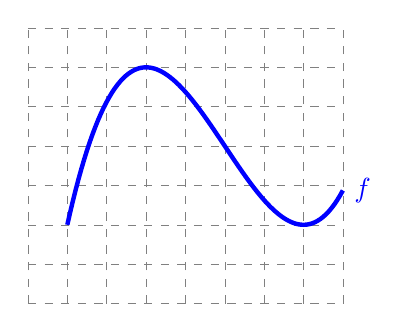
\begin{tikzpicture}[scale =0.5]
\draw[help lines, dashed] (-1,-1) grid (7,6);
\gridlines{-1}{7}{-1}{6};
\draw[ultra thick, blue, domain=0:7, samples=100] plot (\x, {1/8*((\x)^3-12*(\x)^2+36*\x)+1}) node[right] {$f$};
\end{tikzpicture}
\end{center}
\end{multicols}\vspace{-15pt}

The domain is the collection of all possible $x$-values. By inspecting the graph, the horizontal values range between 0 and 7. Thus, $\dom f = [0,7]$. The range is the collection of all possible $y$-values. By inspecting the graph, the vertical values range between 1 and 5. Thus, $\ran f = [1,5]$.  
\end{enumerate}
\end{Exam}\vs

\begin{Exam} Sketch the graph and find the domain and range of each function.
\begin{enumerate}
\begin{multicols}{2}
\item $f(x) = 2x-1$.\\

The graph of $f$ is a line with slope 2 and $y$-intercept $-1$. We see that \fbox{$\dom f = (-\infty, \infty)$} and \fbox{$\ran f = (-\infty, \infty)$}.\vfill

\begin{center}
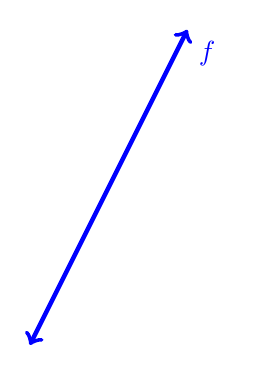
\begin{tikzpicture}[scale =0.5]
\gridlines{-2}{5}{-3}{5};
\draw[ultra thick, blue, <->, domain=-1:3] plot (\x, {2*\x-1}) node[below right] {$f$};
\end{tikzpicture}
\end{center}
\end{multicols}


\begin{multicols}{2}
\item $g(x) = x^2$.\\

The graph of $g$ is a parabola with vertex at the origin and concaves upward. We see that \fbox{$\dom g = (-\infty, \infty)$} and \fbox{$\ran g = [0, \infty)$}.\vfill

\begin{center}
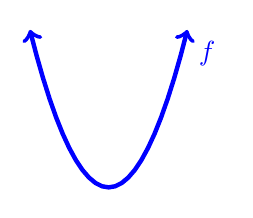
\begin{tikzpicture}[scale =0.5]
\gridlines{-4}{4}{-1}{4};
\draw[ultra thick, blue, <->, domain=-2:2] plot (\x, {(\x)^2}) node[below right] {$f$};
\end{tikzpicture}
\end{center}
\end{multicols}
\end{enumerate}
\end{Exam}\vs

\begin{Exam} Find the domain of each function.
\begin{enumerate}
\item $f(x) = \sqrt{x+2}$.\\

The radicand must be nonnegative, so we solve the inequality $x+2 \ge 0$. This implies that $x \ge -2$. Therefore, \fbox{$\dom f = [-2,\infty)$}. \vs

\item $g(x) = \dfrac{1}{x^2-x}$.\\

Here, we must determine which choices of $x$ make the denominator equal to zero. The domain of $g$ is every real number except these values. We thus solve the equation $x^2-x=0$. This involves factoring.
\[x^2-x = x(x-1)=0.\]  Thus, the solutions are $x=0, 1$. Therefore, \fbox{$\dom g = \{x\mid x\neq 0, 1\} = (-\infty, 0)\cup (0,1)\cup (1,\infty)$}. 
\end{enumerate}
\end{Exam}\vs

\begin{Exam} If $f(x) = 2x^2-5x+1$ and $h\neq 0$, evaluate $\dfrac{f(a+h) - f(a)}{h}$.\\
\begin{eqnarray*} 
\dfrac{f(a+h) - f(a)}{h} &=& \dfrac{[2(a+h)^2-5(a+h)+1] - [2a^2-5a+1]}{h}\\
&=& \dfrac{[2(a^2+2ah+h^2)-5(a+h)+1] - [2a^2-5a+1]}{h}\\
&=& \dfrac{[\cancel{2a^2}+4ah+2h^2 -\bcancel{ 5a}-5h +\cancel{1}] - [\cancel{2a^2}-\bcancel{5a}+\cancel{1}]}{h} = \dfrac{4ah+2h^2-5h}{h}\\
& =& \dfrac{h(4a+2h-5)}{h} =\fbox{$4a+2h-5$}. 
\end{eqnarray*}
\end{Exam}\vs

\begin{Exam} When you turn on a hot-water faucet, the temperature $T$ of the water depends on how long the water has been running. Draw a rough graph of $T$ as a function of the time $t$ that has elapsed since the faucet was turned on.
\begin{multicols}{2}
The initial temperature of the running water is close to room temperature because the water has been sitting in the pipes. When the water from the hot-water tank starts flowing from the faucet, $T$ increases quickly. In the next phase, $T$ is constant at the temperature of the heated water in the tank. When the tank is drained, $T$ decreases to the temperature of the water supply. This enables us to make the rough sketch of $T$ as a function of $t$:
\begin{center}
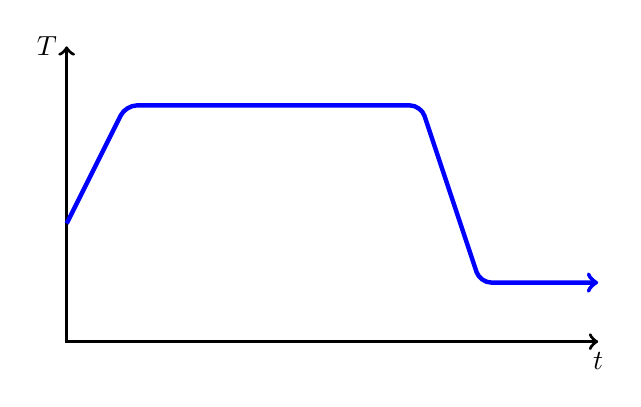
\begin{tikzpicture}[scale = 0.75]
\path (0,0) -- (0,5) node[left] {$T$};
\draw[very thick, <->] (0,5) -- (0,0) -- (9,0) node[below] {$t$};
\draw[ultra thick, blue, rounded corners, ->] (0,2) -- (1,4) -- (6,4) -- (7,1) -- (9,1);
\end{tikzpicture}
\end{center}
\end{multicols}
\end{Exam}\vs

%\begin{Exam} A rectangular storage container with an open top has a volume of 10 $m^3$. The length of its base is twice its width. Material for the base costs $\$10$ per square meter; material for the sides costs $\$6$ per square meter. Express the cost of materials as a function of the width of the base.\\
%
%\[C(w) = 20w^2 + \dfrac{180}{w},\qquad w > 0.\] One application of Calculus will be to determine the minimal cost to manufacture such a box.
%\end{Exam}\vs

\begin{Def} If a function $f$ satisfies $f(-x) = f(x)$ for all $x$ in the domain of $f$, then $f$ is called an \textbf{even function}. If a function $f$ satisfies $f(-x) = -f(x)$ for all $x$ in the domain of $f$, then $f$ is called an \textbf{odd function}.
\end{Def}\vs

These above definitions are an algebraic way of capturing a geometric notation of symmetry. We give now these geometric definitions. A function $f$ is even if its graph is symmetric about the $y$-axis and a function $f$ is odd if its graph is symmetric about the origin, that is, its graph is left unchanged by a rotation of $\pi$ radians ($180^\circ$) around the origin.

\begin{Exam} Determine whether each of the following functions is even, odd, or neither even nor odd.
\begin{enumerate}
\begin{multicols}{2}
\item $f(x) = x^5+x$
\[f(-x) = (-x)^5+(-x) = -x^5-x = -(x^5+x) = -f(x)\]
Thus, \fbox{$f$ is odd}.\vfill\columnbreak
\begin{center}
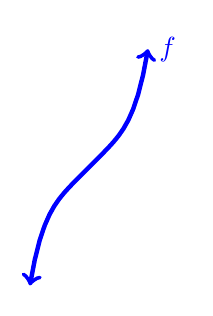
\begin{tikzpicture}[scale=0.75]
\gridlines{-2}{2}{-2}{2};
\draw[ultra thick, blue, <->, domain=-1:1] plot (\x, {(\x)^5+\x}) node[right] {$f$};
\end{tikzpicture}
\end{center}
\end{multicols}
\begin{multicols}{2}
\item $g(x) = 1-x^4$
\[g(-x) = 1-(-x)^4= 1-x^4 = g(x)\]
Thus, \fbox{$g$ is even}.\vfill\columnbreak
\begin{center}
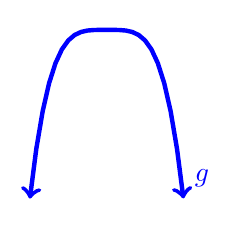
\begin{tikzpicture}[scale=0.75]
\gridlines{-2}{2}{-2}{2};
\draw[ultra thick, blue, <->, domain=-1.3:1.3] plot (\x, {1-(\x)^4}) node[above right] {$g$};
\end{tikzpicture}
\end{center}
\end{multicols}
\begin{multicols}{2}
\item $h(x) = 2x-x^2$ 
\[h(-x) = 2(-x)-(-x)^2 = -2x-x^2 \neq -h(x), h(-x)\]
Thus, \fbox{$h$ is neither even nor odd}.\vfill\columnbreak
\begin{center}
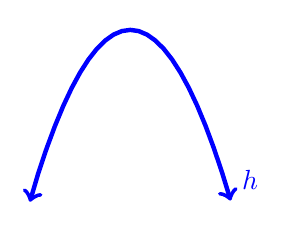
\begin{tikzpicture}[scale=0.75]
\gridlines{-1}{3}{-2}{2};
\draw[ultra thick, blue, <->, domain=-0.7:2.7] plot (\x, {2*\x1-(\x)^2}) node[above right] {$h$};
\end{tikzpicture}
\end{center}
\end{multicols}

\end{enumerate}
\end{Exam}\vs

\begin{Def} Let $f$ be a function defined on some interval. Then for any two numbers $x_1$ and $x_2$ in the interval, $f$ is \textbf{increasing} on the interval if 
\[f(x_1) < f(x_2),\;\;\mbox{whenever}\;\; x_1< x_2,\] and $f$ is \textbf{decreasing} on the interval if \[f(x_1) > f(x_2),\;\;\mbox{whenever}\;\; x_1< x_2.\]
\end{Def}\vs

%The graph of a function can sometimes be all over the place. In particular, on certain intervals the function may be increasing and on other intervals it may be decreasing. How can we tell from the equation that defines a function where the graph is increasing and where it is decreasing?\\
%
%%\centerline{\includegraphics[scale=1.]{../../Pictures/function0.png}}\vs
%
%If $f(x) = mx +b$ is a linear function, then the slope of $f(x)$, namely $m$, tells us if the line is increasing or decreasing. It depends whether $m$ is positive or negative; $f(x)$ is increasing when $m> 0$ and decreasing when $m < 0$. Also, $f(x)$ is neither increasing nor decreasing when $m =0$.  Thus, slope is an algebraic measure of finding the increasing and decreasing intervals of a linear function. How can we talk about the slope of a nonlinear function? We will see later in the semester that Calculus will be a useful tool for answering this question.\\

\vfill
\footnotetext[1]{See \href{https://cnx.org/contents/i4nRcikn@3.7:fP4FUrwS@7/Review-of-Functions}{\S 1.1 Review of Functions} in OpenStax Calculus Volume 1 for additional reading.}
\pagebreak

\startExercises{functions}
\startHW
% Exam 1 #10
For Exercises \ref{function:graph:start}--\ref{function:graph:stop}, the graphs of $f$ and $g$ are illustrated.
\columnratio{0.65}
\begin{paracol}{2}
\begin{enumerate}[!HW!]
\item\label{function:graph:start} Find the domain and range of $f$.\\
\item Find the domain and range of $g$.\\
\item Evaluate $g(0)$.\\
\item Solve $f(x)=3$.\\
\item Solve $f(x)=g(x)$.\\
\item\label{function:graph:stop} On what intervals is $f$ decreasing?\\
\end{enumerate}
\switchcolumn
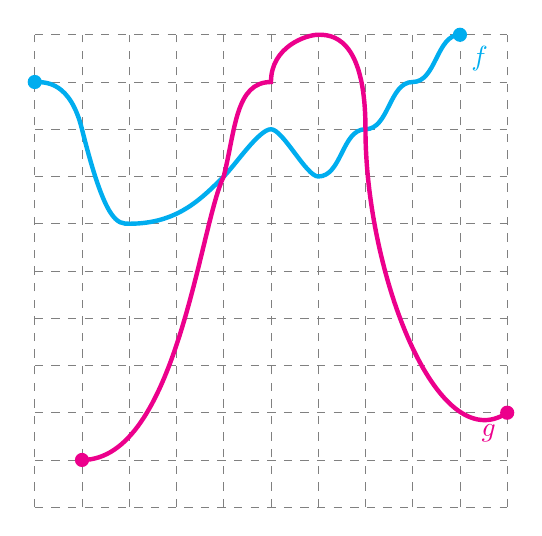
\begin{tikzpicture}[scale=0.6]
\draw[help lines, dashed] (-5,-5) grid (5,5);
\gridlines{-5}{5}{-5}{5};
\draw[ultra thick, cyan] (-5,4) .. controls (-4.75,4) and (-4.25,4) .. (-4,3) 
.. controls (-3.5,1) and (-3.25,1) .. (-3,1) 
.. controls (-2,1) and (-1.5,1.5) .. (-1,2) 
.. controls (-0.75,2.25) and (-0.25,3)  .. (0,3) 
.. controls (0.25,3) and (0.75,2) .. (1,2) 
.. controls (1.5,2) and (1.5,3) .. (2,3)
.. controls (2.5,3) and (2.5,4) .. (3,4)
.. controls (3.5,4) and (3.5,5) .. (4,5) node[below right] {$f$};
\draw[ultra thick, magenta] (-4,-4) .. controls (-2,-4) and (-1.5,1) .. (-1,2) 
.. controls (-0.75,3) and (-0.75,4) .. (0,4)
.. controls (0,4.75) and (0.75,5) .. (1,5)
.. controls (1.25,5) and (2,5) .. (2,3) 
.. controls (2,0) and (3.5,-4) .. (5,-3) node[below left] {$g$};
\fill[cyan] (-5,4) circle(0.15) (4,5) circle(0.15);
\fill[magenta] (-4,-4) circle(0.15) (5,-3) circle(0.15);
\end{tikzpicture}
\end{paracol}

\begin{enumerate}[!HW!]
\begin{multicols}{2}
\itemspade In the function $f$ illustrated below, on what intervals is $f$ increasing?
\begin{center}
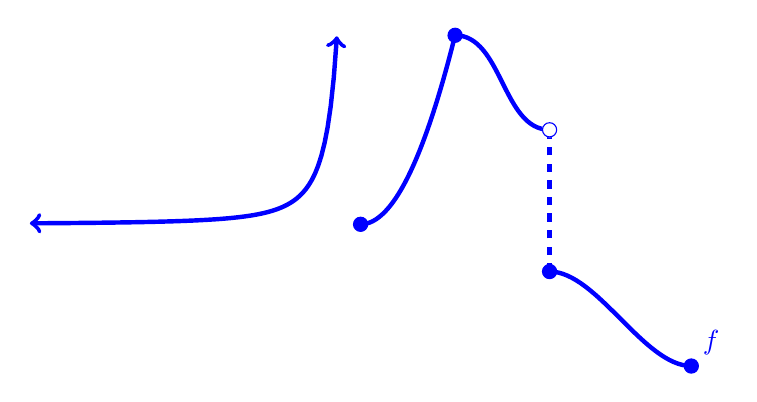
\begin{tikzpicture}[scale = 0.6]
\gridlines{-7}{7}{-3}{5};
\draw[ultra thick, blue, samples= 100, domain=-7:-0.5, <->] plot (\x, {1/(\x)^2+1});
\draw[ultra thick, blue, samples= 100, domain=0:2] plot (\x, {(\x)^2+1});
\draw[ultra thick, blue] (2,5) .. controls (3,5) and (3,3) .. (4,3);
\draw[ultra thick, blue] (4,0) .. controls (5,0) and (6,-2) .. (7,-2) node[above right] {$f$};
\draw[ultra thick, blue, dashed] (4,0) -- (4,3);
\draw[white, fill] (4,3) circle (0.15);
\draw[blue] (4,3) circle (0.15);
\draw[blue, fill] (0,1) circle (0.15);
\draw[blue, fill] (2,5) circle (0.15);
\draw[blue, fill] (4,0) circle (0.15);
\draw[blue, fill] (7,-2) circle (0.15);
\end{tikzpicture}
\end{center}
\end{multicols}
\end{enumerate}

% Exam 1 #5
For Exercises \ref{exer:evenfunction:start}--\ref{exer:evenfunction:stop},  determine analytically if the function is even, odd, or neither.  Justify your response.
\begin{enumerate}[!HW!]
\begin{multicols}{4}
\item \label{exer:evenfunction:start} $f(x) = x^5-x$ 
\item  $g(x) = x^4-1$ 
\itemspade $h(x) = \sqrt[3]{x}$ 
\itemspade $f(x) = \sqrt[3]{2x^2+1}$ 
\end{multicols}
\begin{multicols}{4}
\itemspade $g(x) = x^{1/2}$ 
\item $h(x) = x^{1/3}$ 
\item $f(x) = x^{1/4}$ 
\item $g(x) = \dfrac{1}{x}$ 
\end{multicols}
\begin{multicols}{4}
\item $h(x) = \dfrac{1}{x^2}$ 
\item $f(x) = x+\dfrac{4}{x}$ 
\item $f(x) = \dfrac{x}{x^2+1}$
\itemspade $g(x) = \dfrac{x}{x^2+x+1}$ 
\end{multicols}
\begin{multicols}{4}
\itemspade $h(x)=x|x|$ 
\item\label{exer:evenfunction:stop} $f(x) = \dfrac{2x}{|x|}$ 
\end{multicols}
\end{enumerate}

% Exam 1 #14
For Exercises \ref{exer:domain:start}--\ref{exer:domain:stop},  find the domain of the function. 
\begin{enumerate}[!HW!]
\begin{multicols}{3}
\item\label{exer:domain:start} $f(x) =\dfrac{2x+1}{x^2-1}$
\item $f(x) = \dfrac{(3x-1)(2x+7)}{(x+2)(5x+4)}$
\item $f(x) = \dfrac{(x+2)(5x+4)}{(3x-1)(2x+7)}$
\end{multicols}
\begin{multicols}{3}
\item  $f(x) = \dfrac{x^2+3x+2}{x^2+4x+4}$
\item $f(x) = \dfrac{x^2+2x+1}{x^2-1}$
\item $f(x) = \sqrt{2x+1}$
\end{multicols}
\begin{multicols}{3}
\item $g(x) = \sqrt{3-x}-\sqrt{2+x}$
\itemspade $f(x) = \sqrt{2-\sqrt{x}}$
\item $h(x)=\dfrac{4}{\sqrt{x^2-6x}}$
\end{multicols}
\begin{multicols}{3}
\itemspade  $h(x)=\dfrac{1}{\sqrt[4]{x^2-5x}}$ 
\item\label{exer:domain:stop} $f(x) = \dfrac{\sqrt{2x+1}}{x^2-1}$
\end{multicols}
\end{enumerate}

% Exam 1 #15
For Exercises \ref{exer:differencequotient:start}--\ref{exer:differencequotient:stop}, given the function $f$, evaluate and simplify the difference quotient $\dfrac{f(a+h)-f(a)}{h}$, where $h\neq 0$. 
\begin{enumerate}[!HW!]
\begin{multicols}{3}
\item\label{exer:differencequotient:start}  $f(x) = x^2$ 
\item  $f(x) = 2x^2+1$ 
\itemspade  $f(x)=5-9x$ 
\end{multicols}
\begin{multicols}{3}
\itemspade $f(x) = 4+2x-x^2$ 
\itemspade $f(x) = 5x^2-x+3$ 
\item $f(x) = 2x^2+x+1$ 
\end{multicols}
\begin{multicols}{3}
\itemspade $f(x) = \dfrac{7}{x+4}$ 
\item\label{exer:differencequotient:stop} $f(x) = x^3$
\end{multicols}
\end{enumerate}
\pagebreak

\subsection*{Deeper Dive}\mbox{}
For Exercises \ref{exer:factorpolynomial:start}--\ref{exer:factorpolynomial:stop}, factor the polynomial.
\begin{enumerate}[!HW!]
\begin{multicols}{2}
\item\label{exer:factorpolynomial:start} $x^2+2x-8$  %$(x-2)(x+4)$
\item\label{exer:factorpolynomial:stop} $2x^2+5x-3$ %$(2x-1)(x+3)$
\end{multicols}
\end{enumerate}

For Exercises \ref{exer:solvepolynomial:start}--\ref{exer:solvepolynomial:stop}, solve the equation.
\begin{enumerate}[!HW!]
\begin{multicols}{2}
\item\label{exer:solvepolynomial:start} $2x^3+3x^2-2x-3=0$ %$x=1, -1, -\dfrac{3}{2}$
\item\label{exer:solvepolynomial:stop} $2x^{10/3}+3x^{7/3}-2x^{4/3}-3x^{1/3}=0$ %$x=0, 1, -1, -\dfrac{3}{2}$
\end{multicols}
\end{enumerate}

For Exercises \ref{exer:differencequotientquiz:start}--\ref{exer:differencequotientquiz:stop}, simplify the expression, e.g., rationalize the deonominator, clear compounded fractions, reduce to lowest terms.
\begin{enumerate}[!HW!]
\begin{multicols}{3}
\item\label{exer:differencequotientquiz:start} $\sqrt{72x^3y^{10}}$ %$6xy^5\sqrt{2x}$
\item $\sqrt[3]{16x^7y^3z^{11}}$ %$2x^2yz^3\sqrt[3]{2xz^2}$
\item $\dfrac{2}{\sqrt{5}+2}$ %$2\sqrt{5}-4$
\end{multicols}
\begin{multicols}{3}
\item $\dfrac{h}{\sqrt{4+h}-2}$ %$\sqrt{4+h}+2$}$
\item $\dfrac{\frac{1}{y^2}-\frac{1}{xy} -\frac{2}{x^2}}{\frac{1}{y^2}-\frac{3}{xy}+\frac{2}{x^2}}$ %$\dfrac{x+y}{x-y}$
\item\label{exer:differencequotientquiz:stop} $\dfrac{\frac{1}{x+h} - \frac{1}{x}}{h}$ %$-\dfrac{1}{x(x+h)}$
\end{multicols}
\end{enumerate}
\pagebreak

%%%%%%%%%%%% Section 1.2 %%%%%%%%%%%%%%%%%%%%%%%%%%%%%%%%%%%%%%%%%%%%%%%%%%%%%%%%%%
%%%%%%%%%%%%%%%%%%%%%%%%%%%%%%%%%%%%%%%%%%%%%%%%%%%%%%%%%%%%%%%%%%%%%%%%%%%%
\begin{center} 
\emph{``A wise man can learn more from a foolish question than a fool can learn from a wise answer.'' -- Bruce Lee}
\end{center}

\begin{Videos}
\video{https://youtu.be/I47_KIAMMBM}{QR/1210_02_1.png}{Power Functions} &
\video{https://youtu.be/m-eBjL6-6oE}{QR/1210_02_2.png}{Radical Functions}  &
\video{https://youtu.be/A-pzk52o-CY}{QR/1210_02_3.png}{Reciprocal Functions\\ and their Graphs} &
\video{https://youtu.be/LynZejaFSpI}{QR/1210_02_4.png}{Piece-wise Functions}
\end{Videos}

\section{The Library of Algebraic Functions}\label{sec:library}
Calculus is very much a study of continuous functions. To be best equipped for this study, we need to review basic algebraic functions that are used to build more complicated ones.

\begin{multicols}{2}
\textbf{Constant Function} $\qquad f(x) =1$
\begin{eqnarray*}
\dom f &:& (-\infty,\infty)\\
\ran f &:& \{1\}\\
y\text{-intercept} &:& 1\\
x\text{-intercepts} &:& \emptyset\\
\text{symmetry} &:& y\text{-axis}\\
\text{monotonicity}&:& \text{constant on } (-\infty, \infty)\\
\end{eqnarray*}\vfill\columnbreak

\begin{center}
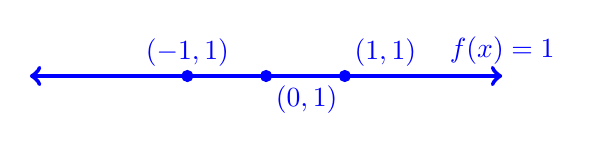
\begin{tikzpicture}
\gridlines{-3}{3}{-2}{2};
\draw[ultra thick, <->, blue, domain=-3:3, samples=100] plot (\x,1) node[above] {$f(x) = 1$};
\draw[fill, blue] (0,1) circle (0.07) node[below right] {$(0,1)$};
\draw[fill, blue] (1,1) circle (0.07) node[above right] {$(1,1)$};
\draw[fill, blue] (-1,1) circle (0.07) node[above] {$(-1,1)$};
\end{tikzpicture}
\end{center}
\end{multicols}\vs

\begin{multicols}{2}
\textbf{Identity Function}  $\qquad f(x) =x$
\begin{eqnarray*}
\dom f &:& (-\infty,\infty)\\
\ran f &:& (-\infty,\infty)\\
y\text{-intercept} &:& 0\\
x\text{-intercepts} &:& \{0\}\\
\text{symmetry} &:& \text{origin}\\
\text{monotonicity}&:& \text{increasing on } (-\infty, \infty)\\
\end{eqnarray*}\vfill\columnbreak

\begin{center}
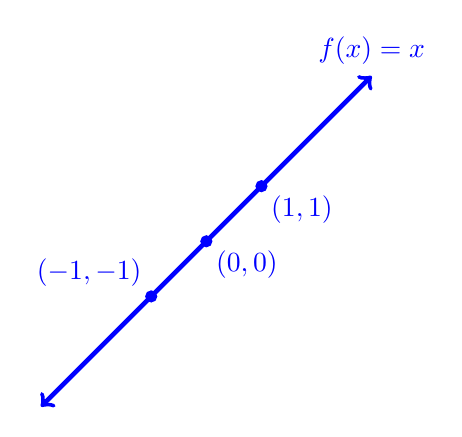
\begin{tikzpicture}[scale = 0.7]
\gridlines{-3}{3}{-3}{3};
\draw[ultra thick, <->, blue, domain=-3:3, samples=100] plot (\x,\x) node[above] {$f(x) = x$};
\draw[fill, blue] (0,0) circle (0.1) node[below right] {$(0,0)$};
\draw[fill, blue] (1,1) circle (0.1) node[below right] {$(1,1)$};
\draw[fill, blue] (-1,-1) circle (0.1) node[above left] {$(-1,-1)$};
\end{tikzpicture}
\end{center}
\end{multicols}

\begin{multicols}{2}
\textbf{Square Function} $\qquad f(x) =x^2$
\begin{eqnarray*}
\dom f &:& (-\infty,\infty)\\
\ran f &:& [0,\infty)\\
y\text{-intercept} &:& 0\\
x\text{-intercepts} &:& \{0\}\\
\text{symmetry} &:& y\text{-axis}\\
\text{monotonicity}&:&  \text{decreasing on } (-\infty, 0);\\
&&\text{increasing on } (0, \infty)
\end{eqnarray*}\vfill\columnbreak

\mbox{}
\begin{center}
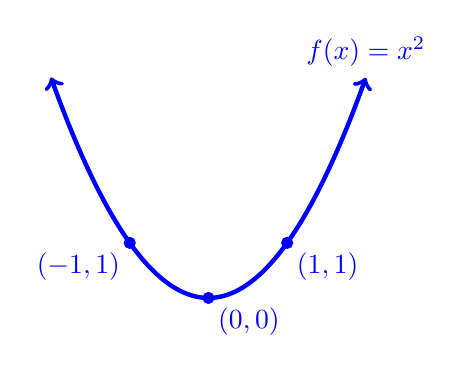
\begin{tikzpicture}[yscale = 0.7]
\gridlines{-3}{3}{-1}{4};
\draw[ultra thick, <->, blue, domain=-2:2, samples=100] plot (\x,{(\x)^2}) node[above] {$f(x) = x^2$};
\draw[fill, blue] (0,0) ellipse (0.07 and 0.1) node[below right] {$(0,0)$};
\draw[fill, blue] (1,1) ellipse (0.07 and 0.1) node[below right] {$(1,1)$};
\draw[fill, blue] (-1,1) ellipse (0.07 and 0.1) node[below left] {$(-1,1)$};
\end{tikzpicture}
\end{center}
\end{multicols}

\begin{multicols}{2}
\textbf{Cube Function} $\qquad f(x) =x^3$
\begin{eqnarray*}
\dom f &:& (-\infty,\infty)\\
\ran f &:& (-\infty,\infty)\\
y\text{-intercept} &:& 0\\
x\text{-intercepts} &:& \{0\}\\
\text{symmetry} &:& \text{origin}\\
\text{monotonicity}&:&  \text{increasing on } (-\infty, \infty)
\end{eqnarray*}
\mbox{}\vfill\columnbreak

\mbox{}
\begin{center}
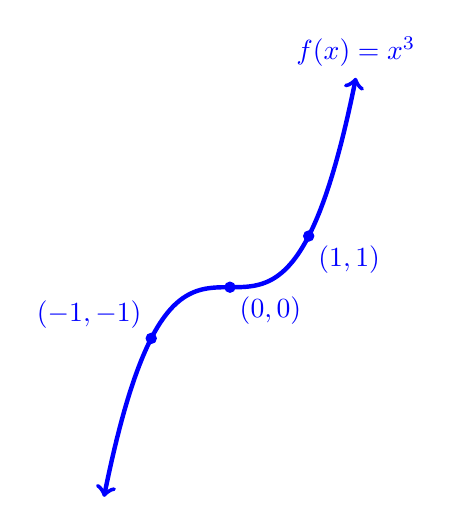
\begin{tikzpicture}[yscale = 0.65]
\gridlines{-3}{3}{-4}{4};
\draw[ultra thick, <->, blue, domain=-1.6:1.6, samples=100] plot (\x,{(\x)^3}) node[above] {$f(x) = x^3$};
\draw[fill, blue] (0,0) ellipse (0.065 and 0.1) node[below right] {$(0,0)$};
\draw[fill, blue] (1,1) ellipse (0.065 and 0.1) node[below right] {$(1,1)$};
\draw[fill, blue] (-1,-1) ellipse (0.065 and 0.1) node[above left] {$(-1,-1)$};
\end{tikzpicture}
\end{center}
\end{multicols}

\begin{multicols}{2}
\textbf{Square Root Function} $\qquad f(x) =\sqrt{x}$
\begin{eqnarray*}
\dom f &:& [0,\infty)\\
\ran f &:& [0,\infty)\\
y\text{-intercept} &:& 0\\
x\text{-intercepts} &:& \{0\}\\
\text{symmetry} &:& \text{none}\\
\text{monotonicity}&:&  \text{increasing on } (0, \infty)\\
\end{eqnarray*}\vfill\columnbreak

\mbox{}
\begin{center}
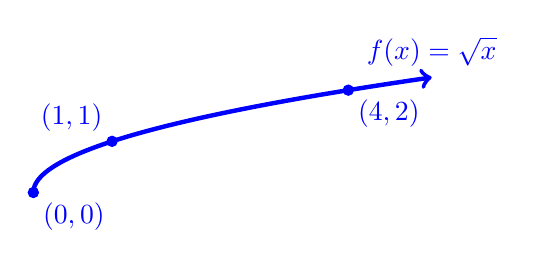
\begin{tikzpicture}[yscale = 0.65]
\gridlines{-1}{5}{-1}{4};
\draw[ultra thick, ->, blue, domain=0:2.25, samples=100] plot ({(\x)^2},\x) node[above] {$f(x) = \sqrt{x}$};
\draw[fill, blue] (0,0) ellipse (0.065 and 0.1) node[below right] {$(0,0)$};
\draw[fill, blue] (1,1) ellipse (0.065 and 0.1)  node[above left] {$(1,1)$};
\draw[fill, blue] (4,2) ellipse (0.065 and 0.1)  node[below right] {$(4,2)$};
\end{tikzpicture}
\end{center}
\end{multicols}

\begin{multicols}{2}
\textbf{Cube Root Function} $\qquad f(x) =\sqrt[3]{x}$
\begin{eqnarray*}
\dom f &:& (-\infty,\infty)\\
\ran f &:& (-\infty,\infty)\\
y\text{-intercept} &:& 0\\
x\text{-intercepts} &:& \{0\}\\
\text{symmetry} &:& \text{origin}\\
\text{monotonicity}&:&  \text{increasing on } (-\infty, \infty)\\
\end{eqnarray*}\vfill\columnbreak

\mbox{}
\begin{center}
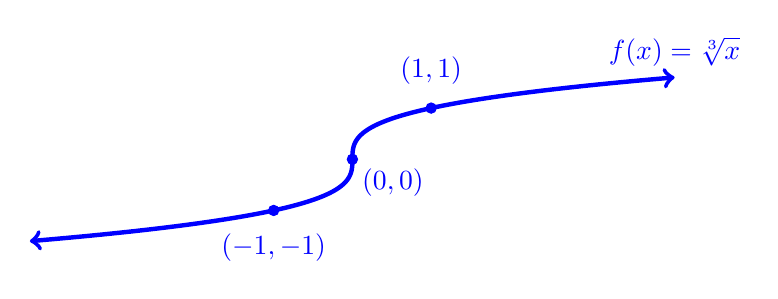
\begin{tikzpicture}[yscale = 0.65]
\gridlines{-4}{4}{-3}{3};
\draw[ultra thick, <->, blue, domain=-1.6:1.6, samples=100] plot ({(\x)^3},\x) node[above] {$f(x) = \sqrt[3]{x}$};
\draw[fill, blue] (0,0) ellipse (0.065 and 0.1) node[below right] {$(0,0)$};
\draw[fill, blue] (1,1) ellipse (0.065 and 0.1)  node[above, yshift=5] {$(1,1)$};
\draw[fill, blue] (-1,-1) ellipse (0.065 and 0.1) node[below, yshift=-5] {$(-1,-1)$};
\end{tikzpicture}
\end{center}
\end{multicols}

\begin{multicols}{2}
\textbf{Reciprocal Function} $\qquad f(x) = \dfrac{1}{x}$
\begin{eqnarray*}
\dom f &:& (-\infty,0)\cup (0,\infty)\\
\ran f &:& (-\infty,0) \cup (0,\infty)\\
y\text{-intercept} &:& \text{none}\\
x\text{-intercepts} &:& \text{none}\\
\text{symmetry} &:& \text{origin}\\
\text{monotonicity}&:&  \text{decreasing on } (-\infty,0)\cup(0,\infty)\\
\end{eqnarray*}\vfill\columnbreak

\mbox{}
\begin{center}
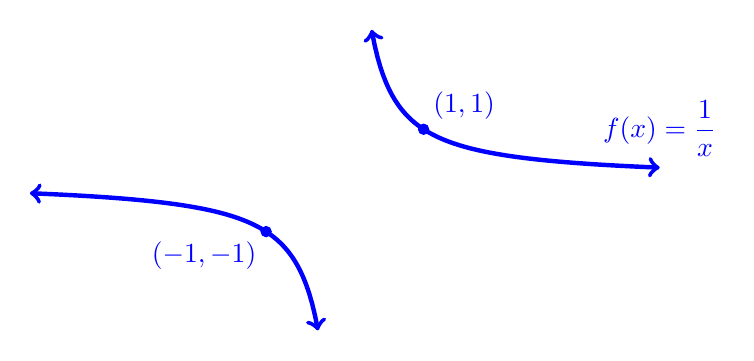
\begin{tikzpicture}[yscale = 0.65]
\gridlines{-4}{4}{-3}{3};
\draw[ultra thick, <->, blue, domain= 0.34:4, samples=100] plot (\x, {1/\x}) node[above] {$f(x) = \dfrac{1}{x}$};
\draw[ultra thick, <->, blue, domain= -4:-0.34, samples=100] plot (\x, {1/\x});
\draw[fill, blue] (1,1) ellipse (0.065 and 0.1) node[above right] {$(1,1)$};
\draw[fill, blue] (-1,-1) ellipse (0.065 and 0.1) node[below left] {$(-1,-1)$};
\end{tikzpicture}
\end{center}
\end{multicols}

\begin{multicols}{2}
\textbf{Absolute Value Function} $\qquad f(x) =|x|$
\begin{eqnarray*}
\dom f &:& (-\infty,\infty)\\
\ran f &:& [0,\infty)\\
y\text{-intercept} &:& 0\\
x\text{-intercepts} &:& \{0\}\\
\text{symmetry} &:& y\text{-axis}\\
\text{monotonicity}&:&  \text{decreasing on } (-\infty, 0);\\
&&\text{increasing on } (0, \infty)
\end{eqnarray*}\vfill\columnbreak

\mbox{}
\begin{center}
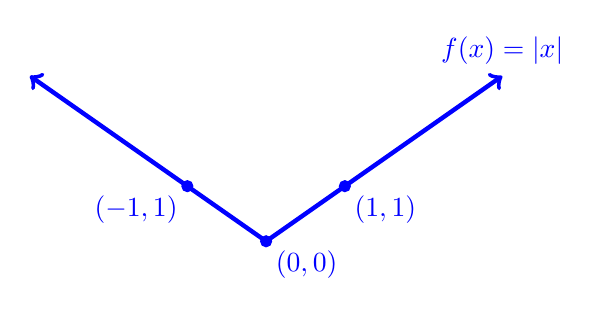
\begin{tikzpicture}[yscale = 0.7]
\gridlines{-3}{3}{-1}{4};
\draw[ultra thick, <->, blue, domain=-3:3, samples=100] plot (\x,{abs(\x)}) node[above] {$f(x) = |x|$};
\draw[fill, blue] (0,0) ellipse (0.07 and 0.1) node[below right] {$(0,0)$};
\draw[fill, blue] (1,1) ellipse (0.07 and 0.1) node[below right] {$(1,1)$};
\draw[fill, blue] (-1,1) ellipse (0.07 and 0.1) node[below left] {$(-1,1)$};
\end{tikzpicture}
\end{center}
\end{multicols}

From these important functions, we can build many more!

\begin{Def} A \textbf{piecewise function} is a function broken into two or more pieces. When reading a piecewise function, the first column provides the function formula and the second determines which $x$-values use which formula. 
\end{Def}\vs

\begin{Exam} Graph the following piecewise functions.
\begin{enumerate}
\begin{multicols}{2}
\item $f(x) = \begin{cases} x+1, & x \neq 1\\ 3, & x=1.\end{cases}$\\

Note that 
\begin{eqnarray*}
f(0) &=& (0)+1 = 1;\\
f(1) &=& 3;\\
f(2) &=& (2)+1 = 3;\\
f(3) &=& (3)+1 = 4.
\end{eqnarray*} \vfill\columnbreak

\begin{center}
\begin{tikzpicture}[scale=0.75]
\gridlines{-3}{3}{-2}{4};
\draw[ultra thick, <->, blue, domain=-3:3, samples=100] plot (\x,{\x+1}) node[above] {$f$};
\draw[fill, gray!10] (1,2) circle (0.1);
\draw[blue, thick] (1,2) circle (0.1);
\draw[fill, blue] (1,3) circle (0.1);
\end{tikzpicture}
\end{center}
\end{multicols}

\begin{multicols}{2}
\item $g(x) = \begin{cases} \sqrt{x-4}, & x \ge 4\\ 8-2x, & x < 4,\end{cases}$\\

Note that 
\begin{eqnarray*}
g(0) &=& 8-2(0) = 8;\\
g(3) &=& 8-2(3) = 2;\\
g(4) &=& \sqrt{(4)-4} = 0;\\
g(8) &=& \sqrt{(8)-4} = 2.
\end{eqnarray*} \vfill\columnbreak

\begin{center}
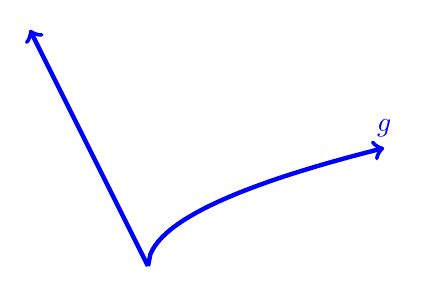
\begin{tikzpicture}[scale =0.75]
\gridlines{-1}{8}{-2}{4};
\draw[ultra thick, <-, blue, domain=2:4, samples=100] plot (\x,{8-2*\x});
\draw[ultra thick, ->, blue, domain=4:8, samples=100] plot (\x,{sqrt(\x-4)}) node[above] {$g$};
\end{tikzpicture}
\end{center}
\end{multicols}

\begin{multicols}{2}
\item $h(x) = \begin{cases} x+1, & x< 1\\ x^2-3x+4,  & 1\le x\le 3\\ 5-x, & x > 3\end{cases}$\\

Note that 
\begin{eqnarray*}
h(0) &=& (0)+1 = 1;\\
h(1) &=& (1)^2-3(1)+4=2;\\
h(3) &=& (3)^2-3(3)+4 = 4.
\end{eqnarray*} \vfill\columnbreak

\begin{center}
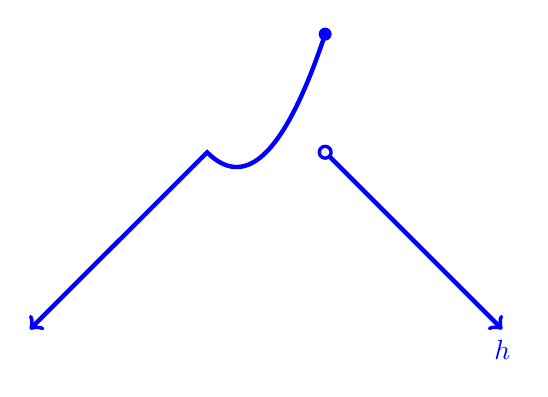
\begin{tikzpicture}[scale =0.75]
\gridlines{-2}{6}{-2}{4};
\draw[ultra thick, blue, domain=3:1, samples=100, ->] plot (\x,{(\x)^2-3*\x+4}) -- (-2,-1);
\draw[ultra thick, ->, blue, domain=3:6, samples=100] plot (\x,{5-\x}) node[below] {$h$};
\draw[fill, blue] (3,4) circle (0.1);
\draw[fill, gray!10] (3,2) circle (0.1);
\draw[blue, very thick] (3,2) circle (0.1);
\end{tikzpicture}
\end{center}
\end{multicols}
\end{enumerate}
\end{Exam}

\vfill
\footnotetext[1]{See \href{https://cnx.org/contents/i4nRcikn@3.7:056cQH8B@7/Basic-Classes-of-Functions}{\S 1.2 Basic Classes of Functions} in OpenStax Calculus Volume 1 for additional reading.}
\pagebreak

\startExercises{library}
\startHW
% Exam 1 #3
For Exercises \ref{exer:library:start}--\ref{exer:library:stop}, which function has its graph illustrated to the right?
\begin{enumerate}[!HW!]
\begin{multicols}{3}
\item\label{exer:library:start} \mbox{}\\
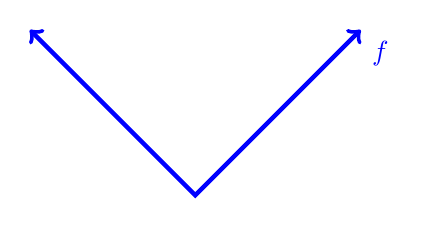
\begin{tikzpicture}[scale = 0.7]
\gridlines{-3}{3}{-3}{3};
\draw[ultra thick, <->, blue, domain=-3:3] plot (\x, {abs(\x)}) node[below right] {$f$};
\end{tikzpicture}
\item \mbox{}\\
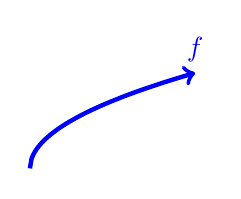
\begin{tikzpicture}[scale = 0.7]
\gridlines{-3}{3}{-3}{3};
\draw[ultra thick, ->, blue, domain=0:3, samples=100] plot (\x, {sqrt(\x)}) node[above] {$f$};
\end{tikzpicture}
\item \mbox{}\\
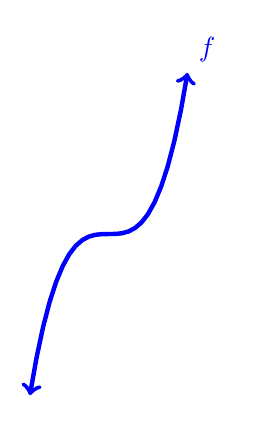
\begin{tikzpicture}[scale = 0.7]
\gridlines{-3}{3}{-3}{3};
\draw[ultra thick, <->, blue, domain=-1.43:1.43] plot (\x, {(\x)^3}) node[above right] {$f$};
\end{tikzpicture}
\end{multicols}

\begin{multicols}{3}
\itemspade \mbox{}\\
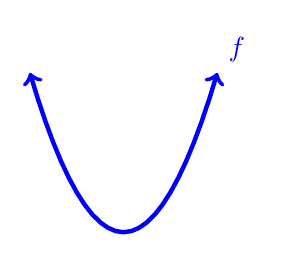
\begin{tikzpicture}[scale = 0.7]
\gridlines{-3}{3}{-3}{3};
\draw[ultra thick, <->, blue, domain=-1.7:1.7] plot (\x, {(\x)^2}) node[above right] {$f$};
\end{tikzpicture}
\itemspade \mbox{}\\
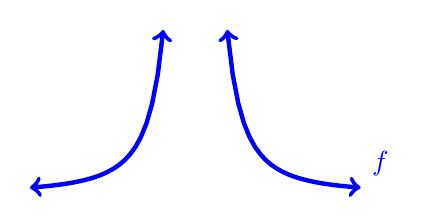
\begin{tikzpicture}[scale = 0.7]
\gridlines{-3}{3}{-3}{3};
\draw[ultra thick, <->, blue, domain=0.58:3] plot (\x, {1/(\x)^2}) node[above right] {$f$};
\draw[ultra thick, <->, blue, domain=-3:-0.58] plot (\x, {1/(\x)^2});
\end{tikzpicture}
\itemspade \mbox{}\\
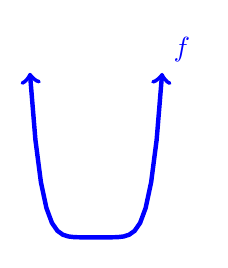
\begin{tikzpicture}[scale = 0.7]
\gridlines{-3}{3}{-3}{3};
\draw[ultra thick, <->, blue, domain=-1.2:1.2] plot (\x, {(\x)^6}) node[above right] {$f$};
\end{tikzpicture}
\end{multicols}

\begin{multicols}{3}
\item \mbox{}\\
\begin{tikzpicture}[scale = 0.7]
\gridlines{-3}{3}{-3}{3};
\draw[ultra thick, <->, blue, domain=-3:3] plot (\x, {(\x)}) node[below right] {$f$};
\end{tikzpicture}

\item \mbox{}\\
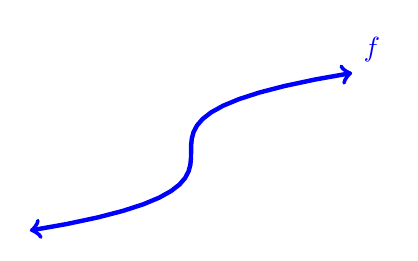
\begin{tikzpicture}[scale = 0.7]
\gridlines{-3}{3}{-3}{3};
\draw[ultra thick, <->, blue, domain=-1.43:1.43] plot ({(\x)^3}, \x) node[above right] {$f$};
\end{tikzpicture}
\item \mbox{}\\
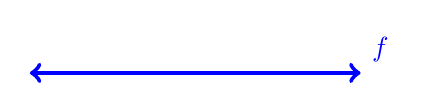
\begin{tikzpicture}[scale = 0.7]
\gridlines{-3}{3}{-3}{3};
\draw[ultra thick, <->, blue, domain=-3:3] plot (\x, 1) node[above right] {$f$};
\end{tikzpicture}
\end{multicols}

\begin{multicols}{2}
\item \mbox{}\\
\begin{tikzpicture}[scale = 0.7]
\gridlines{-3}{3}{-3}{3};
\draw[ultra thick, <->, blue, domain=0.33:3] plot (\x, {1/\x}) node[above right] {$f$};
\draw[ultra thick, <->, blue, domain=-3:-0.33] plot (\x, {1/\x});
\end{tikzpicture}
\item\label{exer:library:stop} \mbox{}\\
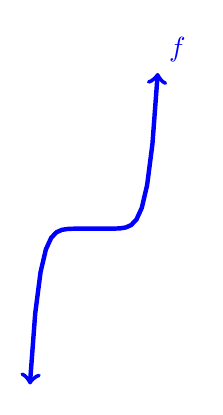
\begin{tikzpicture}[scale = 0.7]
\gridlines{-3}{3}{-3}{3};
\draw[ultra thick, <->, blue, domain=-1.16:1.16] plot (\x, {(\x)^7}) node[above right] {$f$};
\end{tikzpicture}
\end{multicols}
\end{enumerate}


%Exam 1 # 7
For Exercises \ref{exer:piecewise:start}--\ref{exer:piecewise:stop}, the graph of $f$ is provided below. Find a piece-wise function definition for $f$ which matches the graph provided.
\begin{enumerate}[!HW!]
\begin{multicols}{2}
\item\label{exer:piecewise:start} \mbox{}\\
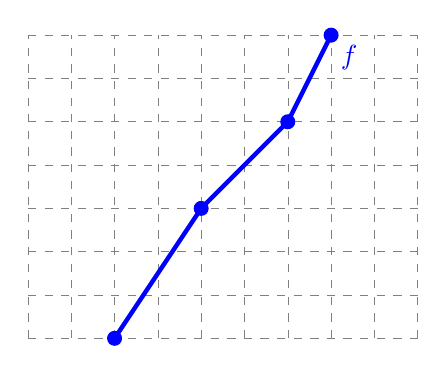
\begin{tikzpicture}[scale=0.55]
\draw[help lines, dashed] (-5,-4) grid (4,3);
\gridlines{-5}{4}{-4}{3};
\draw[ultra thick, blue] (-3,-4) -- (-1,-1)  -- (1,1) -- (2,3);
\draw[blue, fill] (-3,-4) circle (0.16);
\draw[blue, fill] (-1,-1) circle (0.16);
\draw[blue, fill] (1,1) circle (0.16);
\draw[blue, fill] (2,3) circle (0.16) node[below right] {$f$};
\end{tikzpicture}\columnbreak

\itemspade \mbox{}\\
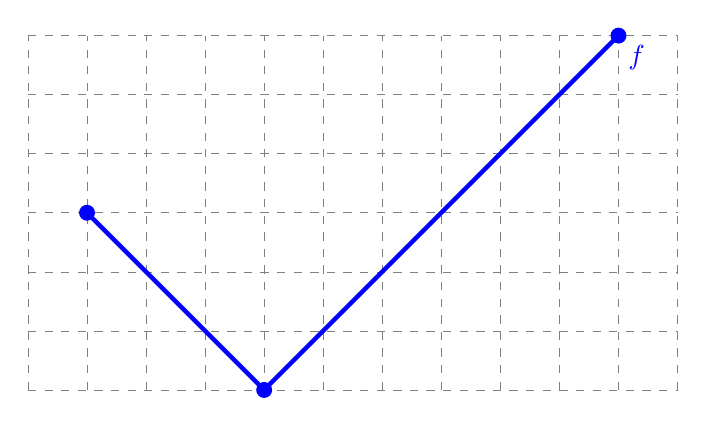
\begin{tikzpicture}[scale =0.75]
\draw[help lines, dashed] (-2,-2) grid (9,4);
\gridlines{-2}{9}{-2}{4};
\draw[ultra thick, blue] (-1,1) -- (2,-2) --  (8,4);
\draw[blue, fill] (-1,1) circle (0.125);
\draw[blue, fill] (2,-2) circle (0.125);
\draw[blue, fill] (8,4) circle (0.125) node[below right] {$f$};
\end{tikzpicture}
\end{multicols}

\begin{multicols}{2}
\itemspade \mbox{}\\
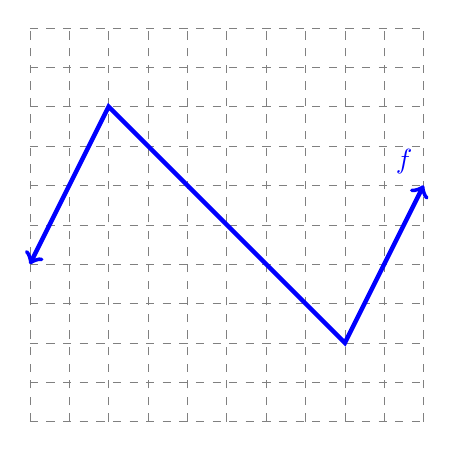
\begin{tikzpicture}[scale=0.5]
\draw[help lines, gray, dashed] (-5,-5) grid (5,5);
\gridlines{-5}{5}{-5}{5};
\draw[ultra thick, blue, <->] (-5,-1) -- (-3,3) -- (3,-3) -- (5,1) node[above , xshift=-7] {$f$};
\end{tikzpicture}\columnbreak

\itemspade \mbox{}\\
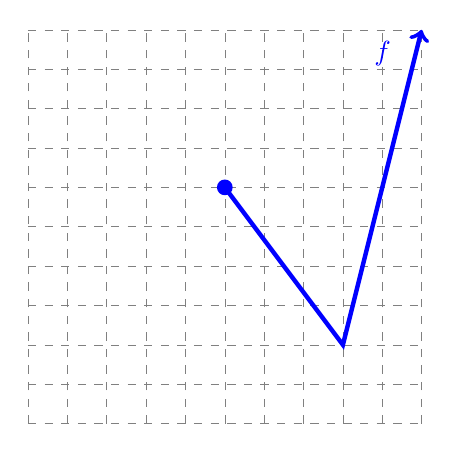
\begin{tikzpicture}[scale=0.5]
\draw[help lines, gray, dashed] (-5,-5) grid (5,5);
\gridlines{-5}{5}{-5}{5};
\fill[blue] (0,1) circle (0.2);
\draw[ultra thick, blue, ->] (0,1) -- (3,-3) -- (5,5) node[below left , xshift=-7] {$f$};
\end{tikzpicture}
\end{multicols}

\begin{multicols}{2}
\item \mbox{}\\
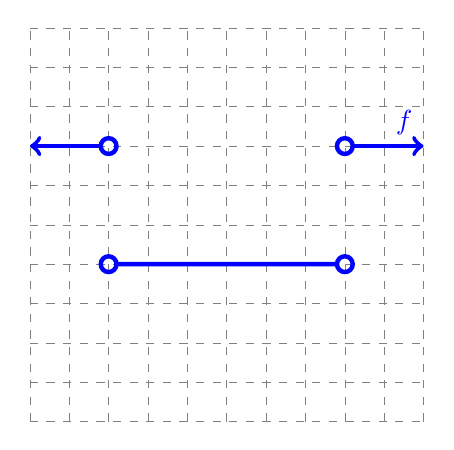
\begin{tikzpicture}[scale=0.5]
\draw[help lines, gray, dashed] (-5,-5) grid (5,5);
\gridlines{-5}{5}{-5}{5};
\draw[ultra thick, blue, <-](-5,2) -- (-3.2,2);
\draw[ultra thick, blue] (-2.8,-1) -- (2.8,-1)
(-3,2) circle (0.2) (3,2) circle (0.2) (-3,-1) circle (0.2) (3,-1) circle (0.2);
\draw[ultra thick, blue, ->] (3.2,2) -- (5,2) node[above, xshift=-7] {$f$};
\end{tikzpicture}

\item\label{exer:piecewise:stop} \mbox{}\\
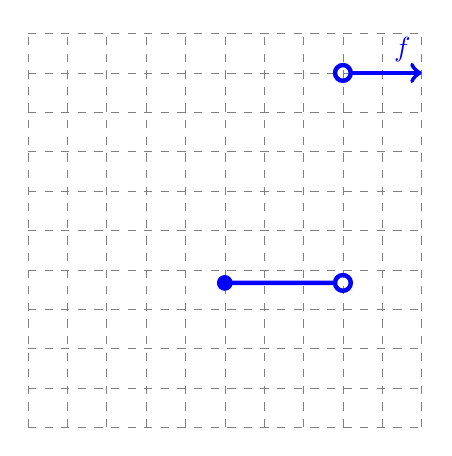
\begin{tikzpicture}[scale=0.5]
\draw[help lines, gray, dashed] (-5,-5) grid (5,5);
\gridlines{-5}{5}{-5}{5};
\fill[blue] (0,-4/3) circle (0.2);
\draw[ultra thick, blue] (0,-4/3) -- (2.8,-4/3)
(3,-4/3) circle (0.2) (3,4) circle (0.2);
\draw[ultra thick, blue, ->] (3.2,4) -- (5,4) node[above, xshift=-7] {$f$};
\end{tikzpicture}
\end{multicols}
\end{enumerate}
\pagebreak

%%%%%%%%%%%% Section 1.3 %%%%%%%%%%%%%%%%%%%%%%%%%%%%%%%%%%%%%%%%%%%%%%%%%%%%%%%%%%
%%%%%%%%%%%%%%%%%%%%%%%%%%%%%%%%%%%%%%%%%%%%%%%%%%%%%%%%%%%%%%%%%%%%%%%%%%%%
\begin{center} 
\emph{``Our character is basically a composite of our habits. Because they are consistent, often unconscious patterns, they constantly, daily, express our character.'' -- Stephen Covey}
\end{center}

\begin{Videos}
\video{https://youtu.be/laW3wkPpcOA}{QR/1210_03_1.png}{Graph Transformations} &
\video{https://youtu.be/RD96z4xykqM}{QR/1210_03_2.png}{Algebra of Functions}  &
\video{https://youtu.be/noRl41eDuPs}{QR/1210_03_3.png}{Function Composition} \\
\video{https://youtu.be/Udfb6zhW-5o}{QR/1210_03_4.png}{Composition of\\ Rational Functions} &
\video{https://youtu.be/Dkg-uQrPhTg}{QR/1210_03_5.png}{Composition of\\ Square Root Functions} &
\video{https://youtu.be/he30d0m4O-M}{QR/1210_03_6.png}{Function Decomposition}
\end{Videos}

\section{Function Composition}\label{sec:compose}
\begin{Prop}[Shifts] Suppose $c > 0$. To obtain the graph of 
\begin{itemize}
\item $y = f(x)+c$, shift the graph of $y=f(x)$ a distance $c$ units upward,
\item $y = f(x)-c$, shift the graph of $y=f(x)$ a distance $c$ units downward.
\item $y = f(x-c)$, shift the graph of $y=f(x)$ a distance $c$ units to the right,
\item $y = f(x+c)$, shift the graph of $y=f(x)$ a distance $c$ units to the left.
\end{itemize}\end{Prop}\vs

\begin{Exam} Let $f(x) = x^2$. Sketch the graphs for $g(x) = x^2+3$ and $h(x) = x^2-3$.\\

\begin{center}
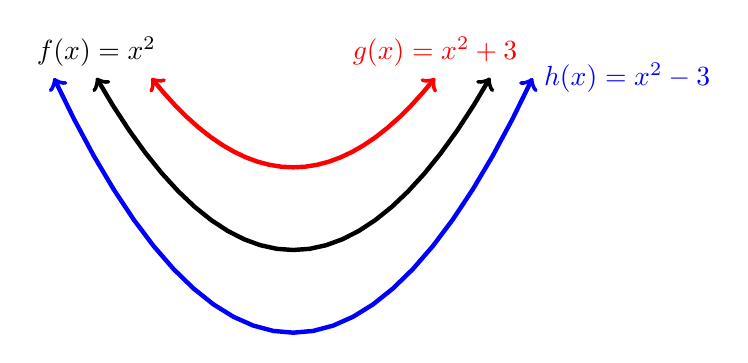
\begin{tikzpicture}[yscale=0.35]
\gridlines{-3}{3}{-4}{6}
\draw[ultra thick, <->, black, domain=2.5:-2.5] plot (\x, {(\x)^2}) node[above] {$f(x) = x^2$};
\draw[ultra thick, <->, red, domain=-1.8:1.8] plot (\x, {(\x)^2+3}) node[above] {$g(x) = x^2+3$};
\draw[ultra thick, <->, blue, domain=-3.04:3.04] plot (\x, {(\x)^2-3}) node[right] {$h(x) = x^2-3$};
\end{tikzpicture}
\end{center}
\end{Exam}\vs

\begin{Exam} Let $f(x) = x^2$.  Sketch the graphs for $g(x) = (x+4)^2$ and $h(x) = (x-2)^2$.

\begin{center}
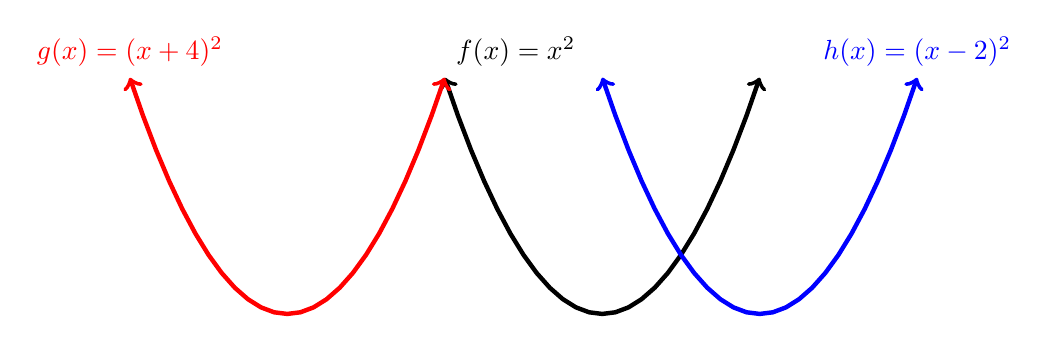
\begin{tikzpicture}[yscale=0.75]
\gridlines{-6}{4}{-1}{4}
\draw[ultra thick, <->, black, domain=2:-2] plot (\x, {(\x)^2}) node[above right] {$f(x) = x^2$};
\draw[ultra thick, <->, red, domain=2:-2] plot (\x-4, {(\x)^2}) node[above] {$g(x) = (x+4)^2$};
\draw[ultra thick, <->, blue, domain=-2:2] plot (\x+2, {(\x)^2}) node[above] {$h(x) = (x-2)^2$};
\end{tikzpicture}
\end{center}
\end{Exam}\vs

\begin{Prop}[Reflections]
To obtain the graph of 
\begin{itemize}
\item $y = -f(x)$, reflect the graph of $y=f(x)$ about the $x$-axis,
\item $y = f(-x)$, reflect the graph of $y=f(x)$ about the $y$-axis,
\item $y = -f(-x)$, rotate the graph of $y=f(x)$ about the origin $\pi$ radians ($180^\circ$).
\end{itemize}
\end{Prop}\vs

\begin{Exam} Let $f(x) = \sqrt{x}$.  Sketch the graphs for $g(x) = -\sqrt{x}$ and $h(x) = \sqrt{-x}$.

\begin{center}
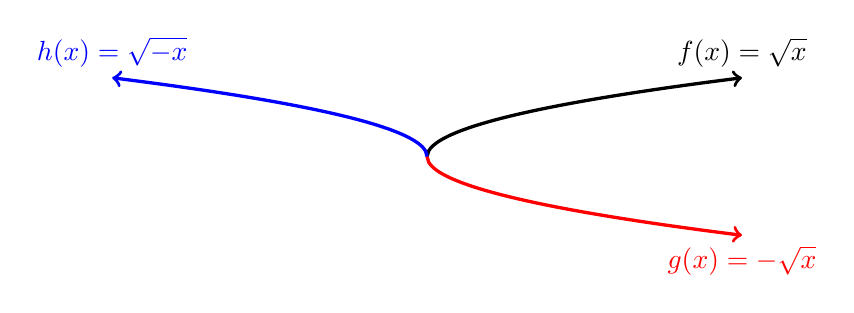
\begin{tikzpicture}[yscale=0.5]
\thicklines
\gridlines{-4}{4}{-2}{2}
\draw[very thick, black, ->, domain=0:4, samples = 200] plot (\x, {sqrt(\x)}) node[above] {$f(x) = \sqrt{x}$};
\draw[very thick, red, ->, domain=0:4, samples = 200] plot (\x, {-sqrt(\x)}) node[below] {$g(x) = -\sqrt{x}$};
\draw[very thick, blue, ->, domain=0:4, samples = 200] plot (-\x, {sqrt(\x)}) node[above] {$h(x) = \sqrt{-x}$};
\end{tikzpicture}
\end{center}
\end{Exam}\vs

\begin{Prop}[Stretches] Suppose that $c > 1$. To obtain the graph
\begin{itemize}
\item $y = cf(x)$, stretch the graph of $y=f(x)$ vertically by a factor of $c$,
\item $y = (1/c)f(x)$, shrink the graph of $y=f(x)$ vertically by a factor of $c$,
\item $y = f(cx)$, shrink the graph of $y=f(x)$ horizontally by a factor of $c$,
\item $y = f(x/c)$, stretch the graph of $y=f(x)$ horizontally by a factor of $c$.
\end{itemize}
\end{Prop}\vs

\begin{Exam} Let $f(x) = |x|$.  Sketch the graphs for $g(x) = 2|x|$ and $h(x) = \frac{1}{2}|x|$.

\begin{center}
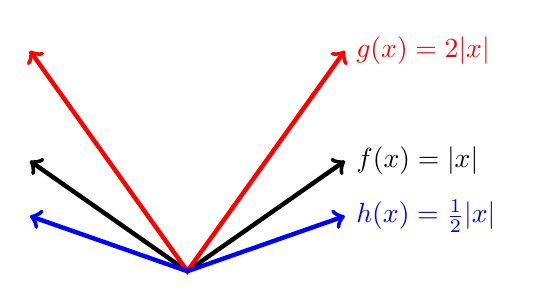
\begin{tikzpicture}[yscale=0.7]
\gridlines{-3}{3}{-1}{4}
\draw[ultra thick, <->, black, domain=-2:2] plot (\x, {abs(\x)}) node[right] {$f(x) = |x|$};
\draw[ultra thick, <->, red, domain=-2:2] plot (\x, {2*abs(\x)}) node[right] {$g(x) = 2|x|$};
\draw[ultra thick, <->, blue, domain=-2:2] plot (\x, {1/2*abs(\x)}) node[right] {$h(x) = \frac{1}{2}|x|$};
\end{tikzpicture}
\end{center}
\end{Exam}\vs

\begin{Exam} Let $f(x) = \sin(x)$.  Sketch the graphs for $g(x) = \sin(2x)$ and $h(x) = \sin\left(\frac{1}{2}x\right)$.\vspace{-15pt}

\begin{center}
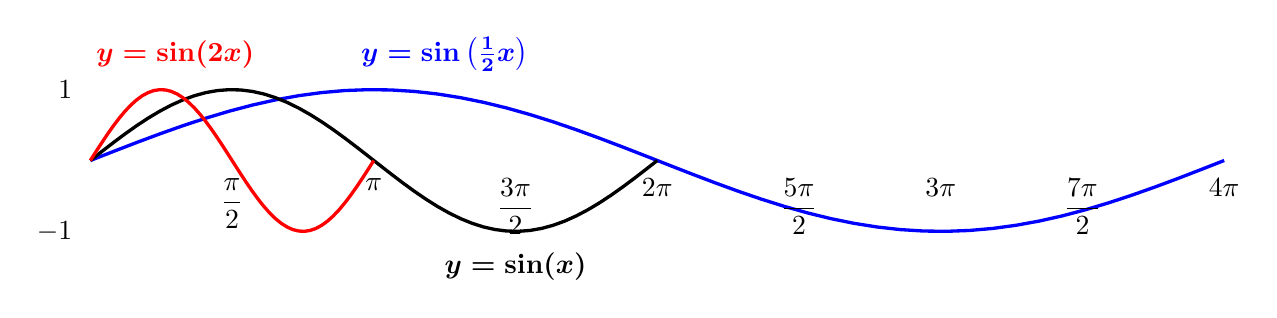
\begin{tikzpicture}[scale=0.9]
\thicklines
\gridlines{-1}{16}{-2}{2}
\draw[very thick, blue, domain=0:16, samples = 50] plot (\x, {sin(deg(pi*\x/8))});
\draw[very thick, black, domain=0:8, samples = 50] plot (\x, {sin(deg(2*pi*\x/8))});
\draw[very thick, red, domain=0:4, samples = 50] plot (\x, {sin(deg(4*pi*\x/8))});
\node[below, yshift = -3] at (2,0) {$\dfrac{\pi}{2}$};
\node[below, yshift = -3] at (4,0) {$\pi$};
\node[below, yshift = -3] at (6,0) {$\dfrac{3\pi}{2}$};
\node[below, yshift = -3] at (8,0) {$2\pi$};
\node[below, yshift = -3] at (10,0) {$\dfrac{5\pi}{2}$};
\node[below, yshift = -3] at (12,0) {$3\pi$};
\node[below, yshift = -3] at (14,0) {$\dfrac{7\pi}{2}$};
\node[below, yshift = -3] at (16,0) {$4\pi$};
\node[left, xshift = -3] at (0,1) {$1$};
\node[left, xshift = -3] at (0,-1) {$-1$};
\node[black] at (6, -1.5) {$\boldsymbol{y=\sin(x)}$};
\node[blue] at (5, 1.5) {$\boldsymbol{y=\sin\left(\frac{1}{2}x\right)}$};
\node[red] at (1.2, 1.5) {$\boldsymbol{y=\sin(2x)}$};
\end{tikzpicture}
\end{center}
\end{Exam}\vs

\begin{Def} Let $f$ and $g$ be functions. Then
\begin{eqnarray*}
(f+g)(x) &=& f(x) + g(x)\qquad \dom (f+g) = \dom f\cap \dom g\\
(f-g)(x) &=& f(x) - g(x)\qquad \dom (f-g) = \dom f\cap \dom g\\
(fg)(x) &=& f(x)g(x)\qquad \dom (fg) = \dom f\cap \dom g\\
(f/g)(x) &=& f(x)/g(x)\qquad \dom (f/g) = (\dom f\cap \dom g)\setminus \{x\mid g(x)=0\}
\end{eqnarray*}
\end{Def}\vs

\begin{Exam}
Let $f(x) = \dfrac{1}{x+2}$ and $g(x) = \dfrac{x}{x-1}$. Then $\dom f = \{x\mid x\neq -2\}$ and $\dom g = \{x\mid x\neq 1\}$.
\begin{eqnarray*}
(f+g)(x) &=& f(x)+g(x) = \dfrac{1}{x+2}+\dfrac{x}{x-1} = \dfrac{1}{x+2}\left(\dfrac{x-1}{x-1}\right)+\dfrac{x}{x-1}\left(\dfrac{x+2}{x+2}\right)\\
 &=&  \dfrac{(x-1) + x(x+2)}{(x-1)(x+2)} = \dfrac{(x-1) + (x^2+2x)}{(x-1)(x+2)} = \fbox{$\dfrac{x^2+3x-1}{(x-1)(x+2)}$}\\
(f-g)(x)  &=&  f(x) - g(x) = \dfrac{(x-1) - x(x+2)}{(x-1)(x+2)} = \dfrac{(x-1) - (x^2+2x)}{(x-1)(x+2)} = \fbox{$-\dfrac{x^2+x+1}{(x-1)(x+2)}$}\\
(fg)(x) &=& f(x)g(x) = \left(\dfrac{1}{x+2}\right)\left(\dfrac{x}{x-1}\right) = \fbox{$\dfrac{x}{(x-1)(x+2)}$}\\
(f/g)(x) &=& \dfrac{f(x)}{g(x)} = \dfrac{1/(x+2)}{x/(x-1)} = \left(\dfrac{1}{x+2}\right)\left(\dfrac{x-1}{x}\right) = \fbox{$\dfrac{x-1}{x(x+2)}$}
\end{eqnarray*}

The domains of $f+g$, $f-g$, and $fg$ are $\{x\mid x\neq 1,-2\}$. The domain of $f/g$ is $\{x\mid x\neq 1,-2,0\}$.
\end{Exam}\vs

\begin{Def} Given two functions $f$ and $g$, the \textbf{composite function} $f\circ g$ is defined by \[(f\circ g)(x) = f(g(x)).\] The domain of $f\circ g$ is the set of all $x$ in the domain of $g$ such that $g(x)$ is in the domain of $f$, that is, $\dom f\circ g = \{x \in \dom g\mid g(x) \in \dom f\}$.
\end{Def}\vs

\begin{Exam} Let $f(x) = x^2+1$ and $g(x) = x-3$. Then compute:\\
\begin{enumerate}
\item $(f\circ g)(x) = f(g(x)) = f(x-3) = (x-3)^2 +1 = (x^2-6x+9)+1 = \fbox{$x^2-6x+10$}$.\\ 

Since the domain of both $f$ and $g$ are all real numbers, the domain of $f\circ g$ is also all real numbers.\\

\item $(g\circ f)(x) = g(f(x)) = f(x) - 3 = (x^2+1)-3 = \fbox{$x^2-2$}$.\\

Since the domain of both $f$ and $g$ are all real numbers, the domain of $g\circ f$ is also all real numbers.
\end{enumerate}
\end{Exam}\vs

\begin{Exam} Let $f(x) = \sqrt{x}$ and let $g(x) = \sqrt{2-x}$. Compute the following composites and their domains:
\begin{enumerate}
\item $(f\circ g)(x) = \sqrt{g(x)} = \sqrt{\sqrt{2-x}} = \fbox{$\sqrt[4]{2-x},\quad \dom f\circ g = (-\infty, 2]$}$.\\

\item $(g\circ f)(x) = \sqrt{2-f(x)} = \fbox{$\sqrt{2-\sqrt{x}},\quad \dom g\circ f = [0,4]$}$.\\

\item $(g\circ g)(x) =  g(g(x)) = \sqrt{2-g(x)} = \fbox{$\sqrt{2-\sqrt{2-x}},\quad \dom g\circ g = [-2,2]$}$.\\
\end{enumerate}
\end{Exam}\vs

\begin{Exam} Let $F(x) = \sqrt[4]{x+9}$. Find two functions $f$ and $g$ such that $F(x) = (f\circ g)(x)$.\\

Let $g(x) = x+9$ and $f(x) = \sqrt[4]{x}$. Then $F = f\circ g$.\\

Notice also that  if $h(x) = \sqrt{x+9}$ and $k(x) = \sqrt{x}$, then $F = k\circ h$. Thus, composition factors are not necessarily unique. 
\end{Exam}\vs

\begin{Exam} Find functions $f$ and $g$ such that $f\circ g = H$ if $H(x) = \dfrac{1}{x+1}$.\\

Let $g(x) = x+1$ and $f(x) = 1/x$. Then $(f\circ g)(x) = H(x)$. 
\end{Exam}

\vfill
\footnotetext[1]{See \href{https://cnx.org/contents/i4nRcikn@3.7:fP4FUrwS@7/Review-of-Functions}{\S 1.1 Review of Functions} and \href{https://cnx.org/contents/i4nRcikn@3.7:056cQH8B@7/Basic-Classes-of-Functions}{\S 1.2 Basic Classes of Functions} in OpenStax Calculus Volume 1 for additional reading.}
\pagebreak

\startExercises{compose}
\startHW
For Exercises \ref{exer:graphcompose:start}--\ref{exer:graphcompose:stop}, the graphs of $f$ and $g$ are illustrated. Evaluate the expression.
\begin{multicols}{5}
\begin{enumerate}[!HW!]
\item\label{exer:graphcompose:start} $f(g(-4))$
\itemspade $g(f(-4))$
\itemspade $(g\circ f)(1)$
\itemspade $(f\circ g)(1)$ 
\item\label{exer:graphcompose:stop} $(f\circ f)(2)$
\end{enumerate}
\vfill
\columnbreak
\begin{center}
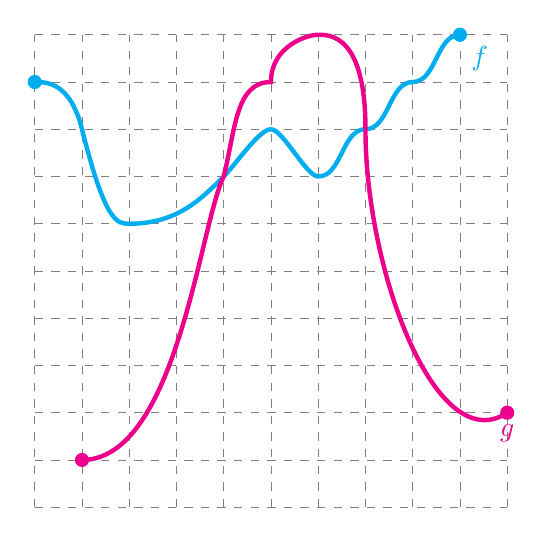
\begin{tikzpicture}[scale=0.6]
\draw[help lines, dashed] (-5,-5) grid (5,5);
\gridlines{-5}{5}{-5}{5};
\draw[ultra thick, cyan] (-5,4) .. controls (-4.75,4) and (-4.25,4) .. (-4,3) 
.. controls (-3.5,1) and (-3.25,1) .. (-3,1) 
.. controls (-2,1) and (-1.5,1.5) .. (-1,2) 
.. controls (-0.75,2.25) and (-0.25,3)  .. (0,3) 
.. controls (0.25,3) and (0.75,2) .. (1,2) 
.. controls (1.5,2) and (1.5,3) .. (2,3)
.. controls (2.5,3) and (2.5,4) .. (3,4)
.. controls (3.5,4) and (3.5,5) .. (4,5) node[below right] {$f$};
\draw[ultra thick, magenta] (-4,-4) .. controls (-2,-4) and (-1.5,1) .. (-1,2) 
.. controls (-0.75,3) and (-0.75,4) .. (0,4)
.. controls (0,4.75) and (0.75,5) .. (1,5)
.. controls (1.25,5) and (2,5) .. (2,3) 
.. controls (2,0) and (3.5,-4) .. (5,-3) node[below] {$g$};
\fill[cyan] (-5,4) circle(0.15) (4,5) circle(0.15);
\fill[magenta] (-4,-4) circle(0.15) (5,-3) circle(0.15);
\end{tikzpicture}
\end{center}
\end{multicols}

For Exercises \ref{exer:functionalg:start}--\ref{exer:functionalg:stop}, for functions $f$ and $g$, find $f+g$, $f-g$, $fg$, and $f/g$ and their respective domains. 
\begin{enumerate}[!HW!]
\item\label{exer:functionalg:start}\label{exer:functionalg:stop} $f(x)=x^3+3x^2$, $g(x)=5x^2-3$
\end{enumerate}

For Exercises \ref{exer:transformexplain:start}--\ref{exer:transformexplain:stop}, explain how the graph is obtained from the graph of $y=f(x)$.
\begin{enumerate}[!HW!]
\begin{multicols}{3}
\item\label{exer:transformexplain:start} $y=4f(x)$ 
\item $y=f(4x)$
\itemspade $y=f(x)+4$ 
\end{multicols}
\begin{multicols}{3}
\itemspade $y=f(x+4)$ 
\itemspade $y=-f(x)-1$ 
\item\label{exer:transformexplain:stop} $y = 4f\left(\frac{1}{4}x\right)$ 
\end{multicols}
\end{enumerate}

%Exam 1 #11 
For Exercises \ref{exer:graphtransform:start}--\ref{exer:graphtransform:stop}, graph the function $y=f(x)$. Indicate three points on the graph. Indicate which transformations were applied to basic function from \secref{sec:library} to obtain $f$.
\begin{enumerate}[!HW!]
\begin{multicols}{3}
\item\label{exer:graphtransform:start} $f(x)=-2(x-2)^3 + 3$
\itemspade $f(x) = 2\sqrt{x-2} + 3$
\item\label{exer:graphtransform:stop} $f(x)=\frac{1}{2}(x-1)^5-2$
\end{multicols}
\end{enumerate}

%Exam 1 #4 
For Exercises \ref{exer:compose:start}--\ref{exer:compose:stop}, for functions $f$ and $g$, find $f\circ g$, $g\circ f$, $f\circ f$, and $g\circ g$ and their respective domains. 
\begin{enumerate}[!HW!]
\begin{multicols}{2}
\item\label{exer:compose:start} $f(x) = 2x+4$, $g(x)= 7x+2$
\itemspade $f(x)=x^2-1$, $g(x)=2x+4$ 
\end{multicols}
\begin{multicols}{2}
\itemspade $f(x)=\sqrt{x}$, $g(x)=\sqrt[3]{9-x}$ 
\itemspade $f(x)=x+\dfrac{1}{x}$, $g(x)=\dfrac{x+11}{x+2}$ 
\end{multicols}
\begin{multicols}{2}
\item\label{exer:compose:stop} $f(x) = x^2+4$, $g(x)= \sqrt{x-2}$
\end{multicols}
\end{enumerate}

%Exam 1 #6
For Exercises \ref{exer:decompose:start}--\ref{exer:decompose:stop}, for the function $F$, find functions $f$ and $g$ such that $F(x)  = (f\circ g)(x)$. 
\begin{enumerate}[!HW!]
\begin{multicols}{3}
\item\label{exer:decompose:start} $F(x) = \sqrt[4]{x^2+1}$ 
\itemspade $F(x) = (2x+x^2)^4$ 
\itemspade $F(x) = \sqrt[3]{\dfrac{x}{6+x}}$ 
\end{multicols}
\begin{multicols}{3}
\itemspade $F(x) = \sqrt{(x^3+6)^2-1}$ 
\item $F(x) = 1-\sqrt{x^2+1}$ 
\item $F(x) = \dfrac{1}{x^2+1}$ 
\end{multicols}
\item\label{exer:decompose:stop} $F(x) = \dfrac{x^2}{x^2+1}$ 
\end{enumerate}
\pagebreak

\subsection*{Deeper Dive}\mbox{}
The graphs of $f$ and $g$ are given below:\\
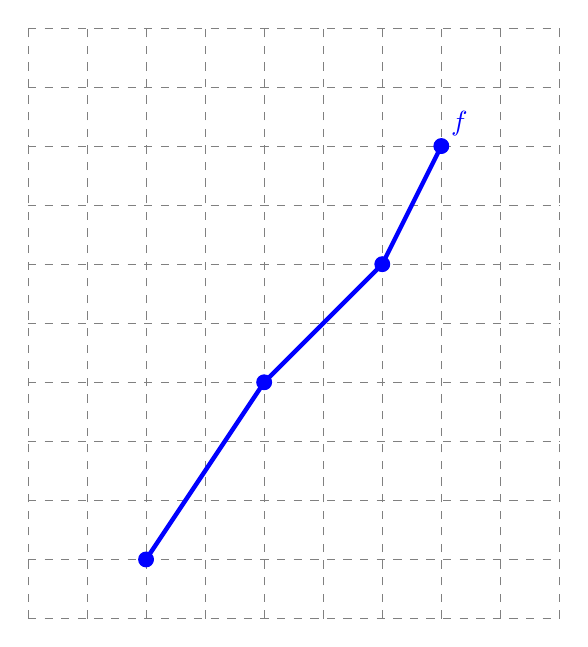
\begin{tikzpicture}[scale =0.75]
\gridlines{-5}{4}{-5}{5};
\draw[help lines, dashed] (-5,-5) grid (4,5);
\draw[ultra thick, blue] (-3,-4) -- (-1,-1)  -- (1,1) -- (2,3);
\draw[blue, fill] (-3,-4) circle (0.125);
\draw[blue, fill] (-1,-1) circle (0.125);
\draw[blue, fill] (1,1) circle (0.125);
\draw[blue, fill] (2,3) circle (0.125) node[above right] {$f$};
\end{tikzpicture}
\hfill
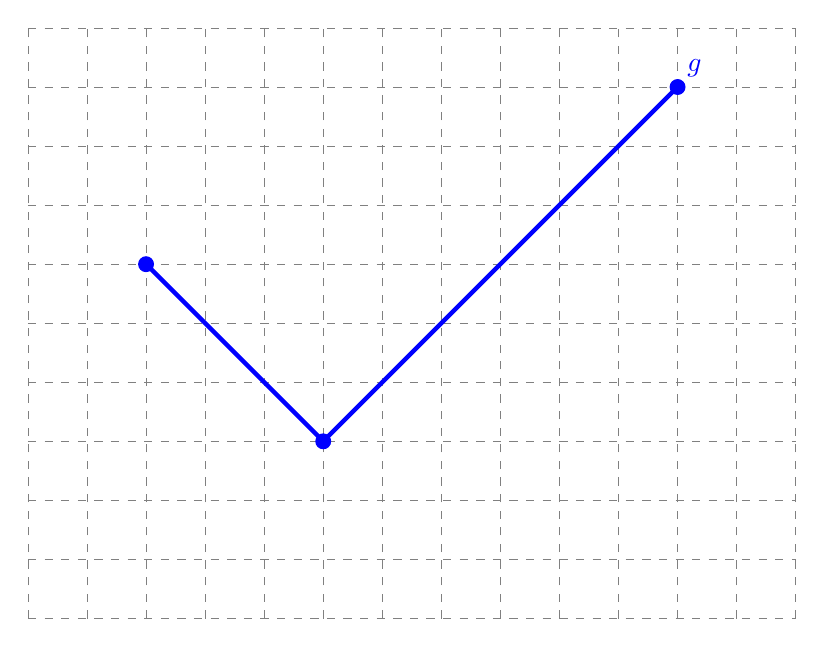
\begin{tikzpicture}[scale =0.75]
\gridlines{-3}{10}{-5}{5};
\draw[help lines, dashed] (-3,-5) grid (10,5);
\draw[ultra thick, blue] (-1,1) -- (2,-2) --  (8,4);
\draw[blue, fill] (-1,1) circle (0.125);
\draw[blue, fill] (2,-2) circle (0.125);
\draw[blue, fill] (8,4) circle (0.125) node[above right] {$g$};
\end{tikzpicture}
\begin{enumerate}[!HW!]
\item Find piece-wise function definitions for $f$ and for $g$ which match the graphs provided above.\\
%\[f(x) = \begin{cases} \frac{3}{2}x+\frac{1}{2} & -3\le x< -1\\ x& -1\le x\le 1\\ 2x-1 & 1< x \le 2\end{cases}\qquad g(x) = \begin{cases} -x & -1\le x< 2\\ x-4 & 2\le x\le 8\end{cases}\]\vs

For Exercises \ref{exer:composegraph:start}--\ref{exer:composegraph:stop}, for the function $F$, find functions $f$ and $g$ such that $F(x)  = (f\circ g)(x)$. 
\begin{multicols}{3}
\item\label{exer:composegraph:start}  $(g\circ f)(2)$ %$-1$
\item $(g\circ f)(-1)$ %$1$
\item\label{exer:composegraph:stop} $(f\circ g)(6)$ %$3$
\end{multicols}

\item Graph $h(x) = -2f(x+1)+2$.\\
%\begin{center}
%\begin{tikzpicture}[scale =0.75]
%\gridlines{-12}{12}{-12}{12};
%\draw[help lines, dashed] (-12,-12) grid (12,12);
%\begin{solution}
%\draw[ultra thick, blue] (-4,10) -- (-2,4) -- (0,0) -- (1,-4);
%\draw[blue, fill] (-4,10) circle (0.15);
%\draw[blue, fill] (-2,4) circle (0.15);
%%\draw[blue, fill] (-1,-2) circle (0.15);
%\draw[blue, fill] (0,0) circle (0.15);
%\draw[blue, fill] (1,-4) circle (0.15) node[below right] {$h$};
%\end{solution}
%\end{tikzpicture}
%\end{center}
\end{enumerate}
\pagebreak
%%%%%%%%%%%% Section 1.4 %%%%%%%%%%%%%%%%%%%%%%%%%%%%%%%%%%%%%%%%%%%%%%%%%%%%%%%%%%
%%%%%%%%%%%%%%%%%%%%%%%%%%%%%%%%%%%%%%%%%%%%%%%%%%%%%%%%%%%%%%%%%%%%%%%%%%%%
\begin{center} 
\emph{``The difference between happiness and misery \ldots often comes down to an error of only a few degrees.''\\ -- Dieter F. Uchtdorf}
%\emph{``The true [sine] of intelligence is not knowledge but imagination.'' -- Albert Einstein}
\end{center}

\begin{Videos}
\video{https://youtu.be/V6jbMhEf7mw}{QR/1210_04_1.png}{Radian Measure} &
\video{https://youtu.be/KJRhDvC6Eck}{QR/1210_04_2.png}{Arc Length}  &
\video{https://youtu.be/_KJcSc4irEo}{QR/1210_04_3.png}{Definitions of the Six\\ Trigonometric Ratios} \\
\video{https://youtu.be/QhkR0j_uQQc}{QR/1210_04_4.png}{Right Triangle\\ Trigonometry} &
\video{https://youtu.be/FJu_wL7E9DA}{QR/1210_04_5.png}{The Unit Circle\\ Diagram} &
\video{https://youtu.be/4DaiN_X380Y}{QR/1210_03_6.png}{The Graph of Sine}
\end{Videos}

\section{Trigonometric Functions}\label{sec:trig}

% In 1979 a large passenger jet with 257 people on board left New Zealand for a sightseeing flight to Antarctica and back. Unknown to the pilots, however, someone had modified the flight coordinates by a mere two degrees. This error placed the aircraft 28 miles (45 km) to the east of where the pilots assumed they were. As they approached Antarctica, the pilots descended to a lower altitude to give the passengers a better look at the landscape. Although both were experienced pilots, neither had made this particular flight before, and they had no way of knowing that the incorrect coordinates had placed them directly in the path of Mount Erebus, an active volcano that rises from the frozen landscape to a height of more than 12,000 feet (3,700 m).\\
%
%As the pilots flew onward, the white of the snow and ice covering the volcano blended with the white of the clouds above, making it appear as though they were flying over flat ground. By the time the instruments sounded the warning that the ground was rising fast toward them, it was too late. The airplane crashed into the side of the volcano, killing everyone on board.\\
%
%It was a terrible tragedy brought on by a minor error --- a matter of only a few degrees.\footnote[2]{See Arthur Marcel, “Mount Erebus Plane Crash,” \url{www.abc.net.au/rn/ockhamsrazor/stories/2007/1814952.htm}.}\\

\begin{Def} \textbf{Trigonometry} is the algebraic study of angles, triangles, circles, and their relationships with each other. An \textbf{angle} is a measurement of how much two intersecting line segments (or rays) differ by rotation.\end{Def}\vs

There are two common ways to measure angles: Degrees and Radians. Comparing degrees with radians, we have the identity $360^\circ = 2\pi\;\mbox{radians}$. Solving for radians, we have \begin{equation} 1\;\mbox{radian} = \left(\dfrac{180^\circ}{\pi}\right).\end{equation} Solving for degrees, we have \begin{equation} 1^\circ = \dfrac{\pi}{180}\;\mbox{radians}\end{equation}

\begin{Exam} Convert degree measures to radians and radian measures to degrees.
\begin{enumerate}
\begin{multicols}{2}
\item $45^\circ = 45\left(\dfrac{\pi}{180}\right) = \dfrac{45\pi}{180} = \fbox{$\dfrac{\pi}{4}$ radians}.$
\item $\dfrac{9\pi}{4}\text{ radians} = \dfrac{9\pi}{4}\left(\dfrac{180^\circ}{\pi}\right) = \fbox{$405^\circ$}.$
\end{multicols}
\end{enumerate}
\end{Exam}\vs

Although radian measure seems more complicated at first glance compared to degree measure, the next example illustrates some of the advantages radians offer.

\begin{Exam} Suppose that we want to calculate the length of an \textbf{arc} of a circle. The arc is bounded by two radii of the circle. These line segments define an angle, which we denote as $\theta$. If the circle has radius length $r$, then the length of the arc, denoted as $s$, follows from the simple formula
\begin{equation}\label{eq:arc}  s = \theta r.\end{equation} Please note that this formula only holds for radian measure!\\

Suppose we have a circle with radius length 1, which is called the \textbf{unit circle}. The \textbf{circumference} of the circle is the arc length of one complete rotation around the circle, that is, the length around the whole circle. Using formula \eqref{eq:arc}, the circumference of the unit circle is $C = 2\pi\cdot 1 = 2\pi$. Furthermore, if  a circle has radius $r$, then the formula for circumference is given as \begin{equation} C = 2\pi r.\end{equation}
\end{Exam}\vs

\begin{Thm}[Pythagorean Theorem]\hspace{- 5 pt}\footnotemark\ In a triangle with a right angle, if the longest side of the triangle (called the hypotenuse) is $r$ and the shorter sides are $x$ and $y$ (called the legs), then \[r^2 = x^2 + y^2.\] \end{Thm}\vs

\begin{Def}
\begin{multicols}{2}
Given the angle $\theta$, consider the diagram, illustrated to the right, where the initial side is the $x$-axis. By the Pythagorean Theorem, we have that $r = \sqrt{x^2+y^2}$. This denotes the distance between the point $(x,y)$ and the origin. From these values: $x$, $y$, and $r$, we define the six  \textbf{trigonometric functions}:
\begin{align*}
\sin \theta &= \dfrac{y}{r} & \cos\theta &= \dfrac{x}{r}  & \tan\theta &= \dfrac{y}{x}= \dfrac{\sin\theta}{\cos\theta}\\
\csc \theta &= \dfrac{r}{y}= \dfrac{1}{\sin\theta} & \sec\theta &= \dfrac{r}{x}= \dfrac{1}{\cos\theta} & \cot\theta &= \dfrac{x}{y}= \dfrac{\cos\theta}{\sin\theta}
\end{align*}  

\begin{center}
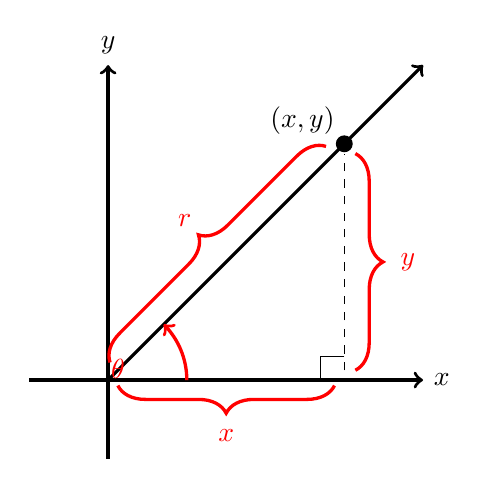
\begin{tikzpicture}
\draw[very thick, ->] (-1,0) -- (4,0) node[right] {$x$};
\draw[very thick, ->] (0,-1) -- (0,4)node[above] {$y$};
\path (3,3) node (P) {}; 
\path (3,0) node (A) {};
\draw[very thick, ->] (0,0) -- (4,4);
\draw[fill] (P) circle (0.1) node[above left]  {$(x,y)$};
\draw[dashed] (A) -- (P);
\draw (3,0.3) -- ++(-0.3,0) -- ++(0,-0.3);
\path (0,0) node (O) {};
\draw[very thick, red, decorate, decoration={ brace, amplitude=10 pt, mirror, raise=2 pt}] (O) -- (A) node[red, midway, yshift = -20 pt] {$x$};
\draw[very thick, red, decorate, decoration={ brace, amplitude=10 pt, mirror, raise=4 pt}] (A) -- (P) node[red, midway, xshift = 23 pt] {$y$};
\draw[very thick, red, decorate, decoration={ brace, amplitude=10 pt, raise=4 pt}] (O) -- (P) node[red, midway, xshift = -15 pt, yshift = 15 pt] {$r$};
\put (1.1,0.4)  {\color{red} $\theta$};
\draw[->, very thick,  red, domain=0:45] plot ({cos(\x)}, {sin(\x)});
\end{tikzpicture}
\end{center} 
\end{multicols}
If $x=0$, then $\sec\theta$ and $\tan\theta$ are undefined. Likewise, if $y=0$, then $\csc\theta$ and $\cot \theta$ are undefined.
\end{Def}\vs

\begin{Exam} 
\begin{multicols}{2}
Consider the following right triangle, illustrated to the right. Substituting the known values $x = 8$ and $y = 15$ in the Pythagorean equation gives \[r = \sqrt{8^2 + 15^2} = \sqrt{64 + 225} = \sqrt{289} = 17.\] We have $x= 8$, $y = 15$, and $r = 17$. The values of the six trigonometric functions of angle $\theta$ are found by using the definitions:
\begin{center}
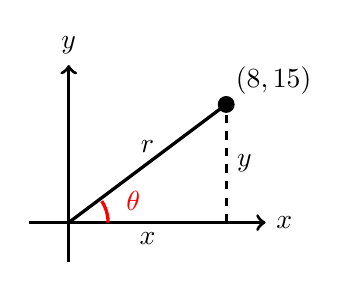
\begin{tikzpicture}[scale=0.5]
\draw[very thick, ->] (-1,0) -- (5,0) node[right] {$x$};
\draw[very thick, ->] (0,-1) -- (0,4) node[above] {$y$};
\draw[ very thick,  red, domain=0:33] plot ({cos(\x)}, {sin(\x)}) node[right, xshift = 5] {$\theta$};
\path (0,0) -- (4,0) node[midway, below] {$x$};
\draw[very thick, dashed] (4,0) -- (4,3) node[midway, right] {$y$};
\draw[very thick] (0,0) -- (4,3) node[midway, above] {$r$};
\draw[fill] (4,3) circle (0.2) node[above right] {$(8,15)$};
\end{tikzpicture}
\end{center}
\end{multicols}

\begin{multicols}{3}
\noindent$\sin\theta = \dfrac{y}{r} = \dfrac{15}{17}$\\\\
$\csc\theta =  \dfrac{r}{y} = \dfrac{17}{15}$\\
$\cos\theta = \dfrac{x}{r} = \dfrac{8}{17}$\\\\
$\sec\theta = \dfrac{r}{x} = \dfrac{17}{8}$\\
$\tan\theta = \dfrac{y}{x} = \dfrac{15}{8}$\\\\
$\cot\theta = \dfrac{x}{y} = \dfrac{8}{15}. $
\end{multicols}
\end{Exam}\vs

Now there are a lot of right triangles with angle $\theta$. So, we may simplify the situation by setting $r=1$. Then the point $(x,y)$ is a point of the unit circle. So, sine measures the $y$-coordinate of any point on the unit circle with respect to a given angle $\theta$. Likewise, cosine measures the $x$-coordinate of any point on the unit circle with respect to a given angle $\theta$. This definition of sine and cosine is just as useful as the definition via right triangles. \\

For your convenience, \figref{fig:unit}\footnotemark\ is a diagram of the unit circle with all the special angles labeled in radians and degrees. You will need to memorize this diagram. Using references angles, it suffices to memorize the first quadrant. In the meanwhile, feel free to use this diagram on your homework. 

\begin{figure}[h]
\begin{center}
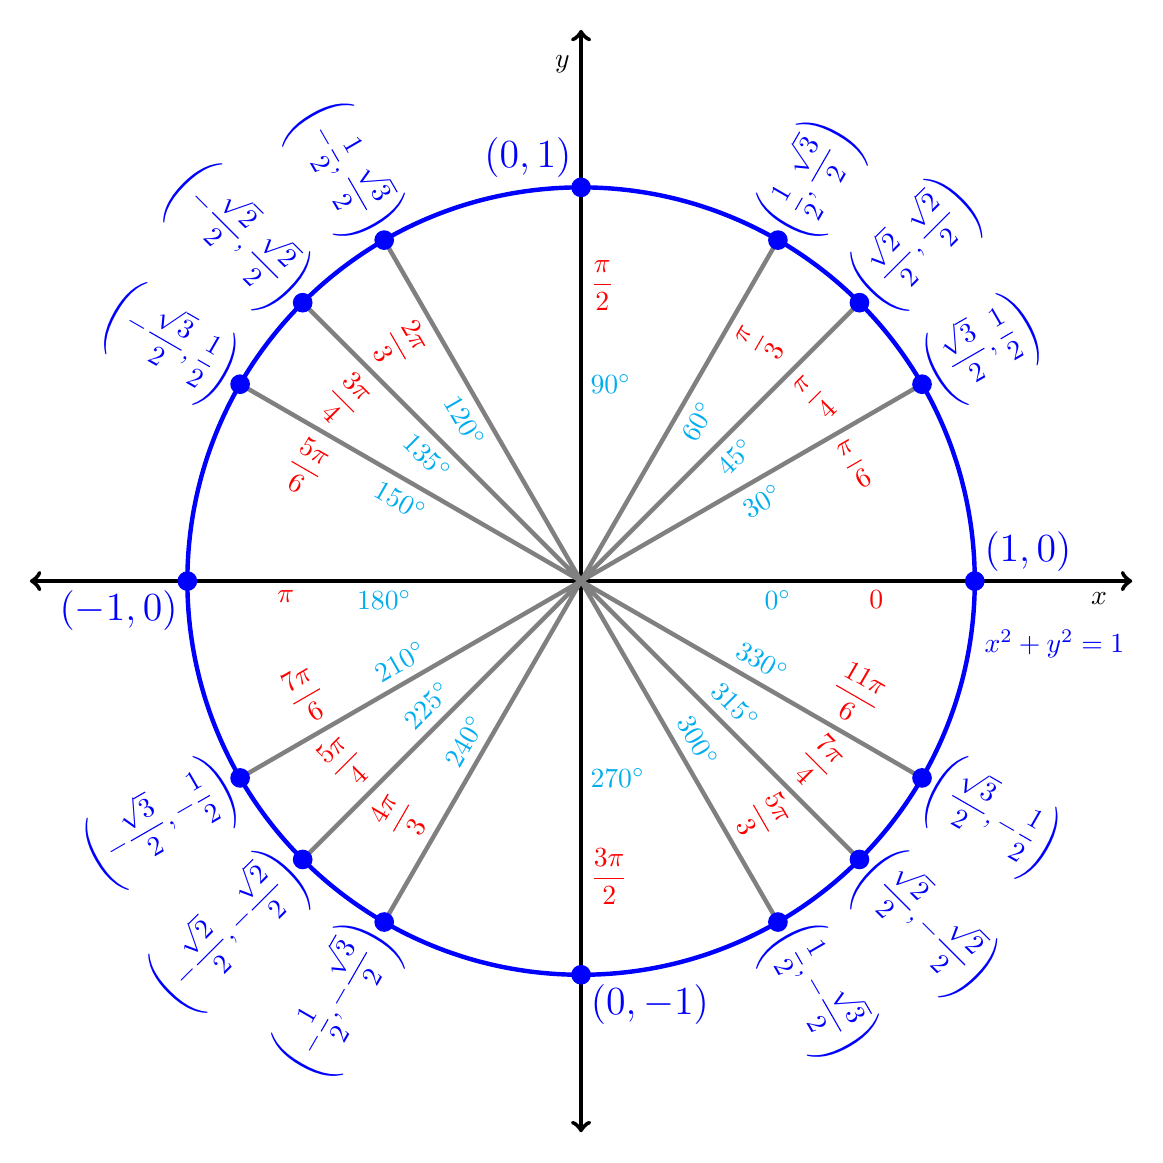
\begin{tikzpicture}
\draw[ultra thick, <->] (-7,0) -- (7,0) node[below left, xshift=-5] {$x$};
\draw[ultra thick, <->] (0,-7) -- (0,7) node[below left, yshift=-5] {$y$};
\draw[help lines, gray, ultra thick] (0,0) -- (30:5) node[below, midway, sloped, cyan] {$30^\circ$} node[below, near end, sloped, red] {$\dfrac{\pi}{6}$}
(0,0) -- (45:5) node[below, midway, sloped, cyan] {$45^\circ$} node[below, near end, sloped, red] {$\dfrac{\pi}{4}$}
(0,0) -- (60:5) node[below, midway, sloped, cyan] {$60^\circ$} node[below, near end, sloped, red] {$\dfrac{\pi}{3}$}
(0,0) -- (150:5) node[below, midway, sloped, cyan] {$150^\circ$} node[below, near end, sloped, red] {$\dfrac{5\pi}{6}$}
(0,0) -- (135:5) node[below, midway, sloped, cyan] {$135^\circ$} node[below, near end, sloped, red] {$\dfrac{3\pi}{4}$}
(0,0) -- (120:5) node[below, midway, sloped, cyan] {$120^\circ$} node[below, near end, sloped, red] {$\dfrac{2\pi}{3}$}
(0,0) -- (210:5) node[above, midway, sloped, cyan] {$210^\circ$} node[above, near end, sloped, red] {$\dfrac{7\pi}{6}$}
(0,0) -- (225:5) node[above, midway, sloped, cyan] {$225^\circ$} node[above, near end, sloped, red] {$\dfrac{5\pi}{4}$}
(0,0) -- (240:5) node[above, midway, sloped, cyan] {$240^\circ$} node[above, near end, sloped, red] {$\dfrac{4\pi}{3}$}
(0,0) -- (330:5) node[above, midway, sloped, cyan] {$330^\circ$} node[above, near end, sloped, red] {$\dfrac{11\pi}{6}$}
(0,0) -- (315:5) node[above, midway, sloped, cyan] {$315^\circ$} node[above, near end, sloped, red] {$\dfrac{7\pi}{4}$}
(0,0) -- (300:5) node[above, midway, sloped, cyan] {$300^\circ$} node[above, near end, sloped, red] {$\dfrac{5\pi}{3}$};
\path[help lines] (0,0) -- (5,0) node[below, midway, cyan] {$0^\circ$} node[below, near end, red] {$0$}
(0,0) -- (0,5) node[right, midway, cyan] {$90^\circ$} node[right, near end, red] {$\dfrac{\pi}{2}$}
(0,0) -- (-5,0) node[below, midway, cyan] {$180^\circ$} node[below, near end, red] {$\pi$}
(0,0) -- (0,-5) node[right, midway, cyan] {$270^\circ$} node[right, near end, red] {$\dfrac{3\pi}{2}$};
\draw[blue, ultra thick] (0,0) circle (5);
\fill[blue] (5,0) circle (0.125) node[above right] {\Large $(1,0)$}
(0,5) circle (0.125) node[above left] {\Large $(0,1)$}
(-5,0) circle (0.125) node[below left] {\Large $(-1,0)$}
(0,-5) circle (0.125) node[below right] {\Large $(0,-1)$}
(30:5) circle (0.125) node[right, rotate=30] {$\left(\dfrac{\sqrt{3}}{2}, \dfrac{1}{2}\right)$}
(45:5) circle (0.125) node[right, rotate=45] {$\left(\dfrac{\sqrt{2}}{2}, \dfrac{\sqrt{2}}{2}\right)$}
(60:5) circle (0.125) node[right, rotate=60] {$\left(\dfrac{1}{2}, \dfrac{\sqrt{3}}{2}\right)$}
(150:5) circle (0.125) node[left, rotate=330] {$\left(-\dfrac{\sqrt{3}}{2}, \dfrac{1}{2}\right)$}
(135:5) circle (0.125) node[left, rotate=315] {$\left(-\dfrac{\sqrt{2}}{2}, \dfrac{\sqrt{2}}{2}\right)$}
(120:5) circle (0.125) node[left, rotate=300] {$\left(-\dfrac{1}{2}, \dfrac{\sqrt{3}}{2}\right)$}
(210:5) circle (0.125) node[left, rotate=30] {$\left(-\dfrac{\sqrt{3}}{2}, -\dfrac{1}{2}\right)$}
(225:5) circle (0.125) node[left, rotate=45] {$\left(-\dfrac{\sqrt{2}}{2}, -\dfrac{\sqrt{2}}{2}\right)$}
(240:5) circle (0.125) node[left, rotate=60] {$\left(-\dfrac{1}{2}, -\dfrac{\sqrt{3}}{2}\right)$}
(330:5) circle (0.125) node[right, rotate=330] {$\left(\dfrac{\sqrt{3}}{2}, -\dfrac{1}{2}\right)$}
(315:5) circle (0.125) node[right, rotate=315] {$\left(\dfrac{\sqrt{2}}{2}, -\dfrac{\sqrt{2}}{2}\right)$}
(300:5) circle (0.125) node[right, rotate=300] {$\left(\dfrac{1}{2}, -\dfrac{\sqrt{3}}{2}\right)$};
\node[below right, blue] at (5,-0.5) {$x^2+y^2=1$};
\end{tikzpicture}
\end{center}
\caption{The Unit Circle}
\label{fig:unit}
\end{figure}



\begin{Exam} Find the following function values without the using a calculator.
\begin{multicols}{2}
\begin{enumerate}
\item $\displaystyle{\cos\dfrac{\pi}{6} = \dfrac{\sqrt{3}}{2}}$\\
\item $\displaystyle{\tan\dfrac{\pi}{3} = \dfrac{\sin \frac{\pi}{3}}{\cos\frac{\pi}{3}} = \dfrac{\sqrt{3}/2}{1/2} = \sqrt{3}}$\\
\item $\displaystyle{\cot\dfrac{\pi}{3} = \dfrac{1}{\tan\frac{\pi}{3}} = \dfrac{1}{\sqrt{3}}}$\\
\item $\displaystyle{\sec\dfrac{2\pi}{3} = \dfrac{1}{\cos\frac{2\pi}{3}} = \dfrac{1}{-1/2} = -2} $
\end{enumerate}
\end{multicols}
\end{Exam}

It will also be necessary for us to remember trigonometric identities and the graphs of the trigonometric functions. Some identities you must know are:
\begin{eqnarray}
\sin^2 x + \cos^2x &=& 1\\
\sin(-x) &=& -\sin (x)\\
\cos(-x) &=& \cos(x)\\
\sin(x+y) &=& \sin(x)\cos(y) + \cos(x)\sin(y)\\
\cos(x+y) &=& \cos(x)\cos(y) - \sin(x)\sin(y)
\end{eqnarray}
Additional important trigonometric identities can be found in the \hyperref[chap:formulas]{appendix}. 

\begin{Exam} Prove the identity: \[\tan^2\alpha - \sin^2\alpha = \tan^2\alpha\sin^2\alpha.\]

When in doubt, one can convert the trigonometric expression into sines and cosines. Starting with the left-hand side we have
\begin{eqnarray*}
\tan^2\alpha - \sin^2\alpha &=& \dfrac{\sin^2\alpha}{\cos^2\alpha} - \sin^2\alpha = \sin^2\alpha\left(\dfrac{1}{\cos^2\alpha} - 1\right) \\
&=& \sin^2\alpha(\sec^2(\alpha) - 1) = \sin^2\alpha\tan^2\alpha. 
\end{eqnarray*}
\end{Exam}\vs

You will also need to know the graphs of the six trigonometric functions, which we add to our library of functions. You will also need to transform them as we did in \secref{sec:library}.


\begin{center}
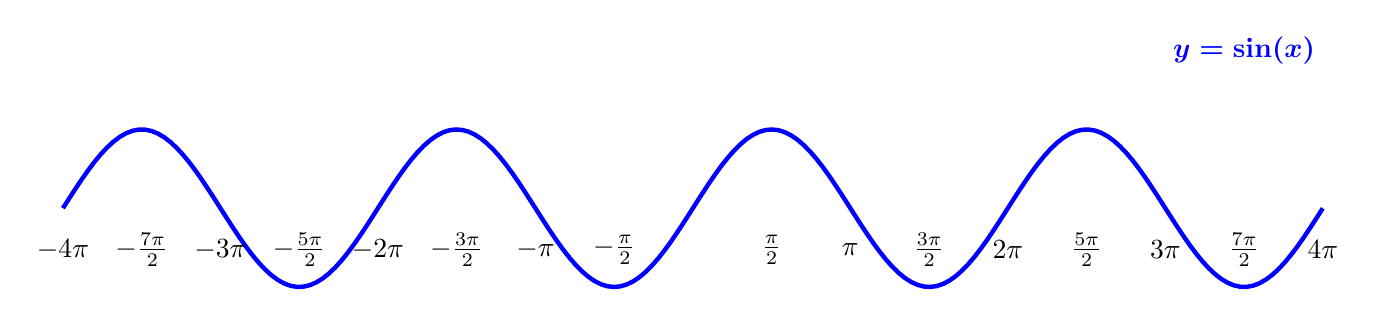
\begin{tikzpicture}
\gridlines{-8}{8}{-2}{2};
\draw[ultra thick, blue, domain=-8:8, samples = 200] plot (\x, {sin(deg(2*pi*\x/4))});
\node[shift={(1,0)}] at (0pt,-15pt) {$\frac{\pi}{2}$};
\node[shift={(2,0)}] at (0pt,-15pt) {$\pi$};
\node[shift={(3,0)}] at (0pt,-15pt) {$\frac{3\pi}{2}$};
\node[shift={(4,0)}] at (0pt,-15pt) {$2\pi$};
\node[shift={(5,0)}] at (0pt,-15pt) {$\frac{5\pi}{2}$};
\node[shift={(6,0)}] at (0pt,-15pt) {$3\pi$};
\node[shift={(7,0)}] at (0pt,-15pt) {$\frac{7\pi}{2}$};
\node[shift={(8,0)}] at (0pt,-15pt) {$4\pi$};
\node[shift={(-1,0)}] at (0pt,-15pt) {$-\frac{\pi}{2}$};
\node[shift={(-2,0)}] at (0pt,-15pt) {$-\pi$};
\node[shift={(-3,0)}] at (0pt,-15pt) {$-\frac{3\pi}{2}$};
\node[shift={(-4,0)}] at (0pt,-15pt) {$-2\pi$};
\node[shift={(-5,0)}] at (0pt,-15pt) {$-\frac{5\pi}{2}$};
\node[shift={(-6,0)}] at (0pt,-15pt) {$-3\pi$};
\node[shift={(-7,0)}] at (0pt,-15pt) {$-\frac{7\pi}{2}$};
\node[shift={(-8,0)}] at (0pt,-15pt) {$-4\pi$};
\node[blue] at (7, 2) {$\boldsymbol{y=\sin(x)}$};
\end{tikzpicture}
\end{center}

\begin{center}
\begin{tikzpicture}
\gridlines{-8}{8}{-2}{2};
\node[shift={(1,0)}] at (0pt,-15pt) {$\frac{\pi}{2}$};
\node[shift={(2,0)}] at (0pt,-15pt) {$\pi$};
\node[shift={(3,0)}] at (0pt,-15pt) {$\frac{3\pi}{2}$};
\node[shift={(4,0)}] at (0pt,-15pt) {$2\pi$};
\node[shift={(5,0)}] at (0pt,-15pt) {$\frac{5\pi}{2}$};
\node[shift={(6,0)}] at (0pt,-15pt) {$3\pi$};
\node[shift={(7,0)}] at (0pt,-15pt) {$\frac{7\pi}{2}$};
\node[shift={(8,0)}] at (0pt,-15pt) {$4\pi$};
\node[shift={(-1,0)}] at (0pt,-15pt) {$-\frac{\pi}{2}$};
\node[shift={(-2,0)}] at (0pt,-15pt) {$-\pi$};
\node[shift={(-3,0)}] at (0pt,-15pt) {$-\frac{3\pi}{2}$};
\node[shift={(-4,0)}] at (0pt,-15pt) {$-2\pi$};
\node[shift={(-5,0)}] at (0pt,-15pt) {$-\frac{5\pi}{2}$};
\node[shift={(-6,0)}] at (0pt,-15pt) {$-3\pi$};
\node[shift={(-7,0)}] at (0pt,-15pt) {$-\frac{7\pi}{2}$};
\node[shift={(-8,0)}] at (0pt,-15pt) {$-4\pi$};
\draw[ultra thick, blue, domain=-8:8, samples = 200] plot (\x, {cos(deg(2*pi*\x/4))});
\node[blue] at (7, -2) {$\boldsymbol{y=\cos(x)}$};
\end{tikzpicture}
\end{center}

\begin{center}
\begin{tikzpicture}[scale=0.85]
\gridlines{-8}{8}{-4}{4};
\draw[fill, blue] (1,1) circle (0.1);
\draw[fill, blue] (0,0) circle (0.1);
\draw[fill, blue] (-1,-1) circle (0.1);
\draw[ultra thick, dashed, red] (2,4) -- (2,-4) node[midway, below right] {$\dfrac{\pi}{2}$};\
\draw[ultra thick, dashed, red] (-2,4) -- (-2,-4) node[midway, below right] {$-\dfrac{\pi}{2}$};
\draw[ultra thick, dashed, red] (6,4) -- (6,-4) node[midway, below right] {$\dfrac{3\pi}{2}$};
\draw[ultra thick, dashed, red] (-6,4) -- (-6,-4) node[midway, below right] {$-\dfrac{3\pi}{2}$};
\draw[ultra thick, <->, blue, domain = -1.69:1.69, samples =50] plot (\x, {tan(deg(pi/4*\x))});
\draw[ultra thick, <->, blue, domain = -1.69:1.69, samples =50] plot (\x+4, {tan(deg(pi/4*\x))});
\draw[ultra thick, <-, blue, domain = -1.69:0, samples =50] plot (\x+8, {tan(deg(pi/4*\x))});
\draw[ultra thick, <->, blue, domain = -1.69:1.69, samples =50] plot (\x-4, {tan(deg(pi/4*\x))});
\draw[ultra thick, ->, blue, domain = 0:1.69, samples =50] plot (\x-8, {tan(deg(pi/4*\x))});
\node[blue] at (4,3) {$\boldsymbol{y=\tan x}$};
\end{tikzpicture}
\end{center}

\begin{center}
\begin{tikzpicture}[scale=0.85]
\gridlines{-8}{8}{-4}{4};
\draw[fill, blue] (1,1) circle (0.1);
\draw[fill, blue] (2,0) circle (0.1);
\draw[fill, blue] (3,-1) circle (0.1);
\draw[ultra thick, dashed, red] (4,4) -- (4,-4) node[midway, below right] {$\pi$};
\draw[ultra thick, dashed, red] (8,4) -- (8,-4) node[midway, below right] {$2\pi$};
\draw[ultra thick, dashed, red] (-4,4) -- (-4,-4) node[midway, below right] {$-\pi$};
\draw[ultra thick, dashed, red] (-8,4) -- (-8,-4) node[midway, below right] {$-2\pi$};
\draw[ultra thick, <->, blue, domain = 0.31:3.69, samples =50] plot (\x, {cot(deg(pi/4*\x))});
\draw[ultra thick, <->, blue, domain = 0.31:3.69, samples =50] plot (\x+4, {cot(deg(pi/4*\x))});
\draw[ultra thick, <->, blue, domain = 0.31:3.69, samples =50] plot (\x-4, {cot(deg(pi/4*\x))});
\draw[ultra thick, <->, blue, domain = 0.31:3.69, samples =50] plot (\x-8, {cot(deg(pi/4*\x))});
\node[blue] at (2,3) {$\boldsymbol{y=\cot x}$};
\end{tikzpicture}
\end{center}

\begin{center}
\begin{tikzpicture}[scale=0.85]
\gridlines{-8}{8}{-4}{4};
\draw[fill, blue] (1,1.41) circle (0.1);
\draw[fill, blue] (0,1) circle (0.1);
\draw[fill, blue] (-1,1.41) circle (0.1);
\draw[fill, blue] (5,-1.41) circle (0.1);
\draw[fill, blue] (4,-1) circle (0.1);
\draw[fill, blue] (3,-1.41) circle (0.1);
\draw[ultra thick, dashed, red] (2,4) -- (2,-4) node[midway, below left] {$\dfrac{\pi}{2}$};\
\draw[ultra thick, dashed, red] (-2,4) -- (-2,-4) node[midway, below left] {$-\dfrac{\pi}{2}$};
\draw[ultra thick, dashed, red] (6,4) -- (6,-4) node[midway, below left] {$\dfrac{3\pi}{2}$};
\draw[ultra thick, dashed, red] (-6,4) -- (-6,-4) node[midway, below left] {$-\dfrac{3\pi}{2}$};
\draw[ultra thick, red, domain = -2:6] plot (\x, {cos(deg(pi/4*\x))});
\draw[ultra thick, <->, blue, domain = -1.69:1.69, samples =50] plot (\x, {sec(deg(pi/4*\x))});
\draw[ultra thick, <->, blue, domain = -1.69:1.69, samples =50] plot (\x+4, {-sec(deg(pi/4*\x))});
\draw[ultra thick, <-, blue, domain = -1.69:0, samples =50] plot (\x+8, {sec(deg(pi/4*\x))});
\draw[ultra thick, <->, blue, domain = -1.69:1.69, samples =50] plot (\x-4, {-sec(deg(pi/4*\x))});
\draw[ultra thick, ->, blue, domain = 0:1.69, samples =50] plot (\x-8, {sec(deg(pi/4*\x))});
\node[red] at (4,-0.5) {$\boldsymbol{y=\cos x}$};
\node[blue] at (4,3) {$\boldsymbol{y=\sec x}$};
\end{tikzpicture}
\end{center}

\begin{center}
\begin{tikzpicture}[scale=0.85]
\gridlines{-8}{8}{-4}{4};
\draw[fill, blue] (1,1.41) circle (0.1);
\draw[fill, blue] (2,1) circle (0.1);
\draw[fill, blue] (3,1.41) circle (0.1);
\draw[fill, blue] (5,-1.41) circle (0.1);
\draw[fill, blue] (6,-1) circle (0.1);
\draw[fill, blue] (7,-1.41) circle (0.1);
\draw[ultra thick, dashed, red] (4,4) -- (4,-4) node[midway, above right] {$\pi$};
\draw[ultra thick, dashed, red] (8,4) -- (8,-4) node[midway, above right] {$2\pi$};
\draw[ultra thick, dashed, red] (-4,4) -- (-4,-4) node[midway, above right] {$-\pi$};
\draw[ultra thick, dashed, red] (-8,4) -- (-8,-4) node[midway, above right] {$-2\pi$};
\draw[ultra thick, red, domain = 0:8] plot (\x, {sin(deg(pi/4*\x))});
\draw[ultra thick, <->, blue, domain = 0.31:3.69, samples =50] plot (\x, {cosec(deg(pi/4*\x))});
\draw[ultra thick, <->, blue, domain = 0.31:3.69, samples =50] plot (\x+4, {-cosec(deg(pi/4*\x))});
\draw[ultra thick, <->, blue, domain = 0.31:3.69, samples =50] plot (\x-4, {-cosec(deg(pi/4*\x))});
\draw[ultra thick, <->, blue, domain = 0.31:3.69, samples =50] plot (\x-8, {cosec(deg(pi/4*\x))});
\node[red] at (2,0.5) {$\boldsymbol{y=\sin x}$};
\node[blue] at (2,3) {$\boldsymbol{y=\csc x}$};
\end{tikzpicture}
\end{center}\vspace{-15pt}

\vfill
\footnotetext[1]{In the Chinese tradition, the Pythagorean Theorem is better known as the \emph{Gougu Rule}\hspace{-1pt}\begin{CJK}{UTF8}{gbsn}
(勾股定理).
\end{CJK}}
%\footnotetext[2]{This image was found on \href{https://en.wikipedia.org/wiki/Unit_circle#/media/File:Unit_circle_angles_color.svg}{Wikipedia} under the article ``Unit Circle'' and is licensed openly.}
\footnotetext[3]{See \href{https://cnx.org/contents/i4nRcikn@3.7:blZd_oDf@5/Trigonometric-Functions}{\S 1.3 Trigonometric Functions} in OpenStax Calculus Volume 1 for additional reading.}
\pagebreak

\startExercises{trig}
\startHW
For Exercises \ref{exer:angleconvert:start}--\ref{exer:angleconvert:stop}, convert each angle from angles to radians or vice versa.
\begin{enumerate}[!HW!]
\begin{multicols}{4}
\item\label{exer:angleconvert:start} $108^\circ$
\item $-210^\circ$
\itemspade $3960^\circ$
\itemspade $67.5^\circ$
\end{multicols}
\begin{multicols}{4}
\itemspade $\dfrac{\pi}{6}$
\itemspade $\dfrac{7\pi}{3}$
\item\label{exer:angleconvert:stop} $3.2$
\end{multicols}
\end{enumerate}

For Exercises \ref{exer:pizzaslice:start}--\ref{exer:pizzaslice:stop}, the graphs of $f$ and $g$ are illustrated. Evaluate the expression.
\begin{enumerate}[!HW!]
\begin{multicols}{3}
\item\label{exer:pizzaslice:start} Find $s$ below.

\vfill
\begin{tikzpicture}[scale=0.65]
\path (130:2.25) node[red] {$s$}
(300:1.5) node {$106^\circ$};
\draw[very thick] (1,0) arc(0:-110:1);
\draw[very thick, blue] (0,0) circle (2);
\draw[ultra thick, red] (2,0) arc(0:250:2) -- (0,0) -- cycle node[midway, above] {$2$};
\end{tikzpicture}
\columnbreak

\itemspade Find $\theta$ below.

\vfill
%\hspace{-30pt}
\begin{tikzpicture}[scale=0.65]
\path (70:2.25) node[red] {$8$}
(70:1.25) node {$\theta$};
\draw[very thick] (1,0) arc(0:140:1);
\draw[very thick, blue] (0,0) circle (2);
\draw[ultra thick, red] (2,0) arc(0:140:2) -- (0,0) -- cycle node[midway, below] {$4$};
\end{tikzpicture}\columnbreak

\item Find the area of the shaded\\ region below.

\vfill
\begin{tikzpicture}[scale=0.65]
\fill[ultra thick, red!50] (2,0) arc(0:60:2) -- (0,0) -- cycle node[midway, below, black] {$8$};
\path (30:1.5) node {$60^\circ$};
\draw[very thick] (1,0) arc(0:60:1);
\draw[very thick, blue] (0,0) circle (2);
\end{tikzpicture}
\end{multicols}\vspace{-10pt}

\begin{multicols}{3}
\itemspade Find the area of the shaded\\ region below.

\vfill
\begin{tikzpicture}[scale=0.65]
\fill[ultra thick, red!50] (2,0) arc(0:23:2) -- (0,0) -- cycle node[midway, below, black] {$10$};
\path (11:1.5) node {$0.4$};
\draw[very thick] (1,0) arc(0:23:1);
\draw[very thick, blue] (0,0) circle (2);
\end{tikzpicture}\columnbreak

\item Find the radius $r$ if the\\ shaded region has area\\ $A=12$ below.

\vfill
\begin{tikzpicture}[scale=0.65]
\fill[ultra thick, red!50] (2,0) arc(0:52:2) -- (0,0) -- cycle node[midway, below, black] {$r$};
\path (26:1.5) node {$0.9$};
\draw[very thick] (1,0) arc(0:52:1);
\draw[very thick, blue] (0,0) circle (2);
\end{tikzpicture}
\columnbreak

\item\label{exer:pizzaslice:stop} Find the radius $r$ if the shaded region has area $A=26$ below.

\vfill
\begin{tikzpicture}[scale=0.65]
\fill[ultra thick, red!50] (2,0) arc(0:120:2) -- (0,0) -- cycle node[midway, below, black] {$r$};
\path (60:1.5) node {$120^\circ$};
\draw[very thick] (1,0) arc(0:120:1);
\draw[very thick, blue] (0,0) circle (2);
\end{tikzpicture}
\end{multicols}\vspace{-10pt}
\end{enumerate}

For Exercises \ref{cw3start}--\ref{cw3stop}, find the exact value of the trigonometric function without a calculator.
\begin{enumerate}[!HW!]
\begin{multicols}{6}
\item\label{cw3start} $\sin \dfrac{2\pi}{3}$
\itemspade $\tan\scalebox{0.8}{$\left(-\dfrac{4\pi}{3}\right)$}$
\itemspade $\sec \dfrac{5\pi}{6}$
\itemspade $\csc\scalebox{0.8}{$\left(-\dfrac{7\pi}{2}\right)$}$
\item $\cot \dfrac{7\pi}{6}$
\item\label{cw3stop} $\cos \dfrac{8\pi}{3}$
\end{multicols}
\end{enumerate}

For Exercises \ref{less4start}--\ref{less4stop}, find all five remaining trigonometric ratios for $\theta$ provided $0<\theta<\dfrac{\pi}{2}$. Find the radian measure of $\angle A$.
\begin{enumerate}[!HW!]
\begin{multicols}{3}
\item\label{less4start} $\tan\theta =\dfrac{28}{96}$
\itemspade $\sin\theta = \dfrac{160}{164}$
\item \label{less4stop} $\tan\theta = \dfrac{60}{32}$
\end{multicols}
\end{enumerate}

For Exercises \ref{exer:graphtrig:start}--\ref{exer:graphtrig:stop}, graph the given function.
\begin{enumerate}[!HW!]
\begin{multicols}{3}
\item\label{exer:graphtrig:start} $f(x) = \sec\left(x-\dfrac{\pi}{4}\right)$
\itemspade $g(x) = \dfrac{1}{2}+\sin(x)$
\item\label{exer:graphtrig:stop} $h(x) = 1+\dfrac{1}{2}\tan x$
\end{multicols}
\end{enumerate}\vfill

\pagebreak
%%%%%%%%%%%% Section 1.5 %%%%%%%%%%%%%%%%%%%%%%%%%%%%%%%%%%%%%%%%%%%%%%%%%%%%%%%%%%
%%%%%%%%%%%%%%%%%%%%%%%%%%%%%%%%%%%%%%%%%%%%%%%%%%%%%%%%%%%%%%%%%%%%%%%%%%%%
\begin{center} 
\emph{``The real energy occurs in each connection between two people, which can bring about exponential returns.'' -- Tom Rath}
\end{center}

\begin{Videos}
\video{https://youtu.be/BFIMHiVS0oU}{QR/1210_05_1.png}{Exponential Laws} &
\video{https://youtu.be/p2b5hYnlhjY}{QR/1210_05_2.png}{Graphs of\\ Exponential Functions}  &
\video{https://youtu.be/dV1pJGe90y4}{QR/1210_05_3.png}{Curve Fitting\\ Exponential Functions} &
\video{https://youtu.be/hgUpB1Zhhoo}{QR/1210_05_4.png}{Exponential Growth} 
\end{Videos}

\section{Exponential Functions}\label{sec:exponent}
\begin{Thm}[Laws of Exponents] If $m, n, a$ and $b$ are real numbers and $a$ and $b$ are positive, then
\begin{multicols}{4}
\begin{enumerate}
\item $a^{m}a^{n} = a^{m+n}$
\item $a^{m}/a^{n} = a^{m-n}$\columnbreak
\item $(a^{m})^n = a^{mn}$%\;\;\; Note that this implies that $(a^m)^n = (a^n)^m$.
\item $(ab)^n = a^nb^n$
%\item $1^n = 1$
\item  $a^0 = 1$
\item $a^{-n} = \dfrac{1}{a^n}$
\item $a^{1/n} = \sqrt[n]{a}$
\item $a^{m/n} = \sqrt[n]{a^m}$
\end{enumerate}
\end{multicols}
 \end{Thm}\vs

The above Law of Exponents allow us to compute $a^x$ for any positive real number $a$ and any rational number $x$. What about $7^{\sqrt{2}}$ or $2^\pi$? Can exponents be computed for irrational numbers?\\

Notice that $\sqrt{3} \approx 1.73205\ldots$, that is, we can approximate $\sqrt{3}$ by an ascending sequence of rational numbers
\[1.7, 1.73, 1.732, 1.7320, 1.73205,\ldots\]
Similarly, we may approximate $a^{\sqrt{3}}$ by the sequence
\[a^{1.7}, a^{1.73}, a^{1.732}, a^{1.7320}, a^{1.73205},\ldots\]
With a lack of calculus and without the proper definition of a limit of a sequence, we accept the fact that this sequence approachs a unique number which we call $a^{\sqrt{3}}$.
For example, \[5^{\sqrt{3}} \approx 5^{1.732} \approx 16.2411.\]

All the rules of exponents apply when the exponents are real (though the proof of this for irrational numbers requires calculus).

\begin{Def} The \textbf{exponential function} of base $a$ (where $a$ is a positive number not equal to 1)  is defined for all real numbers $x$ by \[f(x) = a^x.\]\end{Def}\vs

\begin{Exam} Graph the functions.
\begin{enumerate}
\setlength{\columnsep}{75pt}
\item $\displaystyle{f(x) = 3^x}$.
\begin{center}
\begin{tikzpicture}[yscale=0.425]
\gridlines{-4}{4}{-1}{9};
\draw[ultra thick, blue, <->, domain=-4:2, samples=50] plot (\x, {exp(\x*ln(3)))});
\node[blue] at (-2,4) {$f(x) = 3^x$};
\end{tikzpicture}
\end{center}

\item $\displaystyle{g(x) = 1 - 3^x}$.

\begin{center}
\begin{tikzpicture}[yscale=0.425]
\gridlines{-4}{4}{-10}{1};
\draw[very thick, dashed, red, <->] (-4,1) -- (4,1);
\draw[ultra thick, blue, <->, domain=-4:2, samples=50] plot (\x, {1-exp(\x*ln(3)))});
\node[blue] at (-2,-4) {$g(x) = 1-3^x$};
\end{tikzpicture}
\end{center}
\end{enumerate}
\end{Exam}\vs

\begin{Exam} Find the exponential function satisfying the given conditions.
\begin{enumerate}
\item Find the function $f(x) = a^x$ which passes through $(2,9)$. \\

In particular, we have that
\begin{eqnarray*}
a^2 &=& 9\\
\sqrt{a^2} &=& \sqrt{9}\\
a &=& 3.
\end{eqnarray*}
 So, \fbox{$f(x) = 3^x$}.\\

\item Similarly, find the function $g(x) = a^x$, which passes through $(3,1/8)$.

\begin{eqnarray*}
a^3 &=& \dfrac{1}{8}\\
\sqrt[3]{a^3} &=& \sqrt[3]{\dfrac{1}{8}}\\
a &=& \dfrac{1}{2}.
\end{eqnarray*}
 Thus, \fbox{$g(x)= \left(\dfrac{1}{2}\right)^x$}.\\

\item Find $h(x) = Ca^x$ which passes through $(0,3)$ and $(3,24)$.

\[Ca^0 = C(1) = C = 3\]
So, $h(x) = 3a^x$. But 
\begin{eqnarray*}
3a^3 &=& 24\\
a^3 &=& 8\\
a &=& 2.
\end{eqnarray*} Therefore, \fbox{$h(x) = 3\left(2^x\right)$}. 

\end{enumerate}
\end{Exam}\vs

\begin{Def}Let \[ e \approx 2.71828182845904523536\ldots\]

We call the function $f(x) = e^x$ the \textbf{Natural Exponential Function}.
\end{Def}\vs

We will not go into the details today, but it turns out that $y=e^x$ is the \emph{best} choice for a base of an exponential function. Calculus will reveal this reason.  The natural exponential models various natural phenomena, such population growth, radioactive decay, and interest rates to mention a few.  In particular, we can model uninhibited  growth by the exponential function 
\[P(t) = P_0e^{rt}\] where $P_0$ is the initial ``population'', $t$ is the number of periods of time which have elapsed, and $r$ is the rate of growth with respect to these time units.

\begin{Exam} The initial bacteria count in a culture is 500. A biologist later makes a sample count of bacteria in the culture and finds that the rate of growth is 40\% per hour.
\begin{enumerate}
\item Find a function that models the number of bacteria after $t$ hours.\\

$P_0 = 500, r = 0.40$, and $P(t) = 500e^{0.4t}.$\\

\item What is the estimated amount after 10 hours?

\[P(10) = 500e^{0.4\cdot10} = 500e^4 \approx 500(54.5981) \approx 27,300.\]\vs So we can expect there to by 27,300 bacteria after 10 hours. 
\end{enumerate}
\end{Exam}\vs

\begin{Thm}\label{thm3} For any positive real number $a$ except 1, $f(x) = a^x$ is a one-to-one function. In particular, 
\[\text{if } a^u=a^v, \text{ then } u=v.\]
\end{Thm}\vs

\begin{Exam} Solve the following exponential equations.
\begin{enumerate}
\item $3^{x+1} = 81$. \\

By Theorem \ref{thm3}, if we can write both sides of the equation as a power of 3, then we may conclude that the exponents are the same. In other words, we can \emph{cancel out} the bases on both sides of the equation. We note that $81 = 3^4$. Thus,
\begin{eqnarray*}
3^{x+1} &=& 81\\
3^{x+1} &=& 3^4\\
x+1 &=& 4, \qquad\mbox{by Theorem \ref{thm3}}\\
x &=& \fbox{$3$}.
\end{eqnarray*}

\item $e^{-x^2} = (e^x)^2\cdot \dfrac{1}{e^3}$.\\

Our strategy will be the same, we want to express both sides of the equation as a power of $e$.
\begin{eqnarray*}
e^{-x^2} &=& (e^x)^2\cdot \dfrac{1}{e^3}\\
e^{-x^2} &=& (e^{2x})\cdot e^{-3}\\
e^{-x^2} &=& e^{2x-3}\\
-x^2 &=& 2x-3\\
0 &=& x^2 + 2x-3 = (x+3)(x-1)\\
x &=& \fbox{$1, -3.$}
\end{eqnarray*}
\end{enumerate}
\end{Exam}\vs

\vfill
\footnotetext[1]{See \href{https://cnx.org/contents/i4nRcikn@3.7:TjgBKRr3@9/Exponential-and-Logarithmic-Functions}{\S 1.5 Exponential and Logarithmic Functions} in OpenStax to find the corresponding section.}
\pagebreak

\startExercises{exponent}
\startHW
For Exercises \ref{exer:exponentlaws:start}--\ref{exer:exponentlaws:stop}, simplify the exponential expressions.
\begin{enumerate}[!HW!]
\begin{multicols}{4}
\item\label{exer:exponentlaws:start} $x^8(2x)^7$ 
\item\label{exer:exponentlaws:stop} $\dfrac{(6x^3)^4}{2x^9}$ 
\end{multicols}
\end{enumerate}

%Exam 1 #11
For Exercises \ref{exer:transformexp:start}--\ref{exer:transformexp:stop}, find the formula for $y=f(x)$ by applying the given graph transformation to the basic function $y=e^x$.
\begin{enumerate}[!HW!]
\begin{multicols}{3}
\item\label{exer:transformexp:start} shifting 5 units downward  
\itemspade shifting 4 units to the right 
\itemspade reflecting about the $x$-axis 
\end{multicols}
\begin{multicols}{3}
\item reflecting about the $y$-axis 
\itemspade reflecting about the\\ line $y=6$ 
\itemspade reflecting about the\\ line $x=3$ 
\end{multicols}
\item\label{exer:transformexp:stop} reflecting about the $x$-axis and the $y$-axis\\ 
\end{enumerate}

%Exam 1 #14 
For Exercises \ref{exer:domainexp:start}--\ref{exer:domainexp:stop},  find the domain of the function. 
\begin{enumerate}[!HW!]
\begin{multicols}{4}
\item \label{exer:domainexp:start} $f(x) = \sin(e^{-x})$ 
\itemspade $g(x) = \sqrt{1-5^x}$ 
\itemspade $h(x) = \dfrac{81-e^{x^2}}{1-e^{81-x^2}}$
\item \label{exer:domainexp:stop} $f(x) = \dfrac{4+x}{e^{\cos x}}$ 
\end{multicols}
\end{enumerate}

%Exam 1 #11 
For Exercises \ref{exer:graphtransformexp:start}--\ref{exer:graphtransformexp:stop}, graph the function $y=f(x)$. Indicate which transformations were applied to basic function $y=a^x$ to obtain $f$.
\begin{enumerate}[!HW!]
\begin{multicols}{3}
\item\label{exer:graphtransformexp:start} \label{exer:graphtransformexp:stop} $f(x) = -e^{x-1}+2$ 
\end{multicols}
\end{enumerate}

For Exercises \ref{exer:decomposeexp:start}--\ref{exer:decomposeexp:stop}, for the function $F$, find functions $f$ and $g$ such that $F(x)  = (f\circ g)(x)$. 
\begin{enumerate}[!HW!]
\begin{multicols}{3}
\item \label{exer:decomposeexp:start}\label{exer:decomposeexp:stop} $F(x) = 1-e^{x^2+1}$
\end{multicols}
\end{enumerate}

\begin{enumerate}[!HW!]
\itemspade Find the exponential function $f(x)  = Ca^x$ such that $f(1)=8$ and $f(3)=32$. 
\itemspade Under ideal conditions a certain bacteria population is known to double every four hours. Suppose that there are initially 70 bacteria. What is the size of the population after 8 hours? What is the size of the population after $t$ hours? What is the size of the population after 17 hours? Estimate the time for the population to reach 80,000.

\itemspade A bacteria culture starts with 900 bacteria and doubles in size every half hour. How many bacteria are there after 2 hours? How many bacteria are there after $t$ hours? How many bacteria are there after 40 minutes? Estimate the time for the population to reach 10,000.

\itemspade If $f(x)=e^x$ and $h\neq 0$, then prove that $\dfrac{f(x+h)-f(x)}{h} = e^x\left(\dfrac{e^h-1}{h}\right)$.

\end{enumerate}

\pagebreak
%%%%%%%%%%%% Section 1.6 %%%%%%%%%%%%%%%%%%%%%%%%%%%%%%%%%%%%%%%%%%%%%%%%%%%%%%%%%%
%%%%%%%%%%%%%%%%%%%%%%%%%%%%%%%%%%%%%%%%%%%%%%%%%%%%%%%%%%%%%%%%%%%%%%%%%%%%
\begin{center} 
\emph{``My happiness grows in direct proportion to my acceptance, and in inverse proportion to my expectations.'' -- Michael J. Fox}
\end{center}

\begin{Videos}
\video{https://youtu.be/hrx-WuLXmts}{QR/1210_06_1.png}{One-to-One Functions} &
\video{https://youtu.be/exvthlbr68w}{QR/1210_06_2.png}{Inverse Functions}  &
\video{https://youtu.be/PF_g64F0kq0}{QR/1210_06_3.png}{The Inverse\\ Function Property} &
\video{https://youtu.be/4Sa89VbGk70}{QR/1210_06_4.png}{Computing Inverse\\ Functions Algebraically} \\
\video{https://youtu.be/zHNlny93OR8}{QR/1210_06_5.png}{Finding Inverse Functions\\ of Square Root Functions} &
\video{https://youtu.be/cYMILBgv67I}{QR/1210_06_6.png}{Inverses of\\ Linear Fractionals}  &
\video{https://youtu.be/Eq9B8gEmPjM}{QR/1210_06_7.png}{An Introduction\\ to Logarithms} &
\video{https://youtu.be/EKzE5vv9Wcg}{QR/1210_06_8.png}{Logarithms ARE\\ the Exponents} 
\end{Videos}

\section{Inverse Functions}\label{sec:log}
\begin{Def} A function $f$ is called \textbf{one-to-one} if $f(x_1) = f(x_2)$ implies that $x_1=x_2$.
\end{Def}\vs

Geometrically, a function is one-to-one if it passes the horizontal line test, that is, for every $y$-value, there is  at most one corresponding $x$-value.

\begin{Exam}  By the Horizontal Line Test, $f(x) = x^2$ is not one-to-one but $g(x) = x^3$ is one-to-one. \vspace{-15pt}
\begin{multicols}{2}
\begin{center}
\begin{tikzpicture}[yscale = 0.7]
\gridlines{-3}{3}{-1}{4};
\draw[ultra thick, <->, blue, domain=-2:2, samples=100] plot (\x,{(\x)^2}) node[right] {$f(x) = x^2$};
\draw[thick, red] (-3,1) -- (3,1);
\end{tikzpicture}
\end{center}

\begin{center}
\begin{tikzpicture}[yscale = 0.45]
\gridlines{-3}{3}{-4}{4};
\draw[ultra thick, <->, blue, domain=-1.6:1.6, samples=100] plot (\x,{(\x)^3}) node[right] {$f(x) = x^3$};
\draw[thick, red] (-3,1) -- (3,1);
\draw[thick, red] (-3,2) -- (3,2);
\draw[thick, red] (-3,-1) -- (3,-1);
\draw[thick, red] (-3,-2) -- (3,-2);
\end{tikzpicture}
\end{center}
\end{multicols}
\end{Exam}\vs

\begin{Def}
\begin{multicols}{2}
 If $f$ is a one-to-one function, define $f^{-1}$, the \textbf{inverse function} of $f$, by the formula
\[f^{-1}(y) = x \Longleftrightarrow f(x) = y.\]


In particular, $f^{-1}$ switches all the ordered pairs $(x,y)$ into $(y,x)$. Geometrically, this corresponds to reflecting the graph of $y=f(x)$ across the diagonal line $y=x$. \vfill\columnbreak

\begin{center}
\begin{tikzpicture}[scale=0.5]
\draw[very thin, gray] (-5,-5) grid (5,5);
\gridlines{-5}{5}{-5}{5};
\draw[help lines, very thick, <->, dashed] (-5,-5) -- (5,5);
\draw[ultra thick, red, <->, domain=-3.1:4.12] plot (\x-2, {1/10*(\x)^3-2});
\draw[ultra thick, blue, <->, domain=-3.1:4.12] plot ({1/10*(\x)^3-2},\x-2);
\node[red, ultra thick] at (1.5,4) {$\boldsymbol{f}$};
\node[blue, ultra thick] at (3.5,1) {$\boldsymbol{f^{-1}}$};
\end{tikzpicture}
\end{center}
\end{multicols}
\end{Def}\vs

An important property about inverse functions is how they relate with function composition. 

\begin{equation} (f^{-1}\circ f)(x) = x, \text{ for all } x \text{ in } \dom f, \text{ and } (f\circ f^{-1})(x) = x, \text{ for all } x \text{ in } \ran f.\end{equation}

\begin{Exam} Use the function $f(x) = \sqrt[3]{x-2}$ and its inverse function $f^{-1}(x) = x^3+2$ to find the following:
\begin{enumerate}
\item $f(10) = \sqrt[3]{(10)-2} = \sqrt[3]{8} = \fbox{2}$\\
\item $(f^{-1}\circ f)(10) = f^{-1}(f(10)) = f^{-1}(2) = (2)^3+2 = 8+2 = \fbox{10}$\\
\item $(f^{-1}\circ f)(x) = f^{-1}(\sqrt[3]{x-2}) = (\sqrt[3]{x-2})^3+2 = (x-2) +2 = \fbox{$x$}$
\end{enumerate}
\end{Exam}\vs

To find the algebraic inverse, we simply have to switch the roles of $x$ and $y$ in the defining formula for $f$ and solve for $y$.

\begin{Exam}  Find the algebraic inverse of the function $f(x) = \dfrac{4x-1}{2x+3}$. \\

We first switch $x$ and $y$ and then solve for $y$. 
\begin{eqnarray*}
x &=& \dfrac{4y-1}{2y+3}\\
x(2y+3) &=& 4y-1\\
2xy+3x &=& 4y-1\\
2xy-4y &=& -1-3x\\
y(2x-4) &=& -(3x+1)\\
f^{-1}(x) = y &=& \fbox{$\dfrac{-(3x+1)}{2(x-2)}$}
\end{eqnarray*}
\end{Exam}\vs

For $a > 0$ and $a\neq 1$, we have 

\begin{center}
\begin{tikzpicture}[yscale=0.5]
\gridlines{-4}{4}{-1}{9};
\draw[ultra thick, blue, <->, domain=-4:2, samples=50] plot (\x, {exp(\x*ln(3)))});
\node[blue] at (-2,4) {$f(x) = a^x$};
\end{tikzpicture}
\end{center}

That is, $f(x) = a^x$ is one-to-one. So, $f$ has an inverse function.

\begin{Def} Let $a>0$ and $a\neq 1$. Then the \textbf{Logarithm base} $a$ is the inverse function of $f(x)=a^x$. That is,
\[\log_a(x) = y \Longleftrightarrow a^y = x.\]
\end{Def}\vs
     
\begin{Thm}[Properties of Logarthims] Let $a>0$ and $a\neq1$.
\begin{multicols}{4}
\begin{enumerate}[!THM!]
\item $\log_a1 = 0$
\item $\log_aa = 1$
\item $\log_aa^x = x$
\item $a^{\log_ax}=x$
\end{enumerate}
\end{multicols}
\end{Thm}\vs

We should also mention that $\log_a 0$ is undefined.
      
\begin{Exam} Evaluate the logarithms.
\begin{enumerate}
\begin{multicols}{2}
\item $\log_{10}1000 = \log_{10}10^3 = \fbox{$3$}$
\item $\log_{2}32 = \log_{2}2^5 = \fbox{$5$}$
\end{multicols}
\begin{multicols}{2}
\item $\log_{10}0.1 = \log_{10}10^{-1} = -\fbox{$1$}$
\item $\log_{16}4 = \log_{16}16^{1/2} = \fbox{$1/2$}$
\end{multicols}
\item $\log_{\sqrt{2}} 4 = \log_{\sqrt{2}} \sqrt{2}^4 = \fbox{$4$}$
\end{enumerate}
\end{Exam}\vs

Since $a^x$ and $\log_ax$ are inverses of each other, we can discover the graph of $f(x) = \log_ax$ by reflecting the graph of $g(x) =a^x$ across the line $y=x$. Thus we have 

\begin{center}
\begin{tikzpicture}[yscale=0.5]
\gridlines{-1}{9}{-4}{4};
\draw[ultra thick, blue, <->, domain=-4:2, samples=50] plot ({exp(\x*ln(3)))},\x);
\node[blue] at (2,3) {$f(x) = \log_a(x)$};
\end{tikzpicture}
\end{center}

\begin{Exam} 
 \begin{multicols}{2}
 Sketch the graph of $f(x) = \log_2(x-3)$. Find its domain and range.\\

This is a horizontal shift right by 3 of $y=\log_2 x$. This is a horizontal change, so vertical attributes of $y=\log_2 x$ would not change as we transform into $f$. Thus, $\dom f = (3,\infty)$, $\ran f = (-\infty, \infty)$, and there is a vertical asymptote at $x=3$.

\begin{center}
\begin{tikzpicture}[yscale=0.5, xscale=0.95]
\gridlines{-1}{7}{-4}{4};
\draw[ultra thick, red, <->, dashed] (3,4) -- (3,-4.5);
\draw[ultra thick, blue, <->, domain=0.01:4, samples=200] plot (\x+3, {2+ln(\x)/ln(2)});
\node[blue] at (5,-2) {$f(x) = \log_2(x-3)$};
\end{tikzpicture}
\end{center}
\end{multicols}
\end{Exam}\vs

As we saw earlier, the exponential function $y=e^x$ shows up in applications all the time. Its inverse function is just as useful in calculus and other applications.

\begin{Def} The \textbf{Natural Logarithm} is defined to be \[\ln x = \log_ex\] Most calculators come equipped with a ``LN'' button,\footnotemark\ which evaluates the natural logarithm.
\end{Def}

\vfill
\footnotetext[1]{The abbreviation $\ln$ actually comes from the French ``logarithme naturel,'' which means ``natural logarithm.''}
\footnotetext[2]{See \href{https://cnx.org/contents/i4nRcikn@3.7:Ib8OK9lb@6/Inverse-Functions}{\S 1.4 Inverse Functions} and \href{https://cnx.org/contents/i4nRcikn@3.7:TjgBKRr3@9/Exponential-and-Logarithmic-Functions}{\S 1.5 Exponential and Logarithmic Functions} in OpenStax to find the corresponding sections.}
\pagebreak

\startExercises{log}
\startHW
%Exam 1 #9
For Exercises \ref{exer:onetoone:start}--\ref{exer:onetoone:stop},  which graph correspond to one-to-one function?
\begin{enumerate}[!HW!]
\begin{multicols}{3}
\item\label{exer:onetoone:start} \mbox{}\vspace{-15pt}
\begin{center}
\begin{tikzpicture}[scale=0.5]
\gridlines{-3}{3}{-4}{4};
\draw[ultra thick, <->, blue, domain=-4:4, samples=100] plot (\x,\x);
\end{tikzpicture}
\end{center}
\item\mbox{}\vspace{-15pt}
\begin{center}
\begin{tikzpicture}[scale=0.5]
\gridlines{-3}{3}{-4}{4};
\draw[ultra thick, <->, blue, domain=-2:2, samples=100] plot (\x,{(\x)^2});
\end{tikzpicture}
\end{center}
\item\mbox{}\vspace{-15pt}
\begin{center}
\begin{tikzpicture}[scale=0.5]
\gridlines{-3}{3}{-4}{4};
\draw[ultra thick, <->, blue, domain=-1.6:1.6, samples=100] plot (\x,{(\x)^3});
\end{tikzpicture}
\end{center}
\end{multicols}

\begin{multicols}{3}
\item\mbox{}\vspace{-15pt}
\begin{center}
\begin{tikzpicture}[scale=0.5]
\gridlines{-3}{3}{-4}{4};
\draw[ultra thick, <->, blue, domain=-1.5:1.5, samples=100] plot ({(\x)^3}, \x);
\end{tikzpicture}
\end{center}
\item\mbox{}\vspace{-15pt}
\begin{center}
\begin{tikzpicture}[scale=0.5]
\gridlines{-3}{3}{-4}{4};
\draw[ultra thick, <->, blue, domain=-3:3, samples=100] plot (\x, 1);
\end{tikzpicture}
\end{center}
\item\mbox{}\vspace{-15pt}
\begin{center}
\begin{tikzpicture}[scale=0.5]
\gridlines{-3}{3}{-4}{4};
\draw[ultra thick, <->, blue, domain=0.25:3, samples=100] plot (\x,{1/(\x)});
\draw[ultra thick, <->, blue, domain=-3:-0.25, samples=100] plot (\x,{1/(\x)});
\end{tikzpicture}
\end{center}
\end{multicols}

\begin{multicols}{3}
\itemspade\mbox{}\vspace{-15pt}
\begin{center}
\begin{tikzpicture}[scale=0.5]
\gridlines{-3}{3}{-4}{4};
\draw[ultra thick, <->, blue, domain=0.5:3, samples=100] plot (\x,{1/(\x)^2});
\draw[ultra thick, <->, blue, domain=-3:-0.5, samples=100] plot (\x,{1/(\x)^2});
\end{tikzpicture}
\end{center}
\itemspade\mbox{}\vspace{-15pt}
\begin{center}
\begin{tikzpicture}[scale=0.5]
\gridlines{-3}{3}{-4}{4};
\draw[ultra thick, <->, blue, domain=-3:3, samples=100] plot (\x, {abs(\x)});
\end{tikzpicture}
\end{center}
\itemspade\mbox{}\vspace{-15pt}
\begin{center}
\begin{tikzpicture}[scale=0.5]
\gridlines{-3}{3}{-4}{4};
\draw[ultra thick, <->, blue, domain=-3:1.4, samples=100] plot (\x, {exp(\x)});
\end{tikzpicture}
\end{center}
\end{multicols}

\begin{multicols}{3}
\item\mbox{}\vspace{-15pt}
\begin{center}
\begin{tikzpicture}[scale=0.5]
\gridlines{-3}{3}{-4}{4};
\draw[ultra thick, ->, blue, domain=-0:3, samples=100] plot (\x, {sqrt(\x)});
\end{tikzpicture}
\end{center}
\itemspade\mbox{}\vspace{-15pt}
\begin{center}
\begin{tikzpicture}[scale=0.5]
\gridlines{-3}{3}{-4}{4};
\draw[ultra thick, <->, blue, domain=-3:3, samples=100] plot (\x, {2*cos(deg(\x))});
\end{tikzpicture}
\end{center}
\item\label{exer:onetoone:stop} \mbox{}\vspace{-15pt}
\begin{center}
\begin{tikzpicture}[scale=0.5]
\gridlines{-3}{3}{-4}{4};
\draw[ultra thick, <->, blue, domain=0.02:3, samples=100] plot (\x, {ln(\x)});
\end{tikzpicture}
\end{center}
\end{multicols}
\end{enumerate}

% Exam 1 #14
For Exercises \ref{exer:logdomain:start}--\ref{exer:logdomain:stop},  find the domain of the function. 
\begin{enumerate}[!HW!]
\begin{multicols}{2}
\item\label{exer:logdomain:start} $f(x) = \ln\left(\dfrac{(x+5)^2}{x^2-4}\right)$ 
\itemspade $f(x) = \log_2\left(\dfrac{(x-1)(x+1)}{x+2}\right)$ 
\end{multicols}
\begin{multicols}{2}
\item $f(x) = \ln\left(\dfrac{\sqrt{2x+1}}{x^2-1}\right)$ 
\item \label{exer:logdomain:stop} $f(x)=\dfrac{1+3x}{1-\ln x}$ 
\end{multicols}
\end{enumerate}

%Exam 1 #11 
For Exercises \ref{exer:graphtransformlog:start}--\ref{exer:graphtransformlog:stop}, graph the function $y=f(x)$. Indicate which transformations were applied to basic function $y=\log_a(x)$ to obtain $f$.
\begin{enumerate}[!HW!]
\begin{multicols}{3}
\item\label{exer:graphtransformlog:start} $f(x) = \ln(-x+2)+2$
\item \label{exer:graphtransformlog:stop} $f(x) = \ln(x+2)+2$ 
\end{multicols}
\end{enumerate}

%Exam 1 #12 
For Exercises \ref{exer:inversealg:start}--\ref{exer:inversealg:stop},  find $f^{-1}(x)$, the inverse of $f$. You may assume that $f$ is one-to-one.
\begin{enumerate}[!HW!]
\begin{multicols}{4}
\item\label{exer:inversealg:start} $f(x)= 3x^3-1$ 
\itemspade $f(x)= 3\sqrt[3]{x}-1$ 
\item $f(x)= 2\sqrt[3]{x}+3$
\itemspade $f(x) = 3+\sqrt{5+6x}$ 
\end{multicols}
\begin{multicols}{4}
\itemspade $f(x) = \dfrac{4x-1}{2x+5}$ 
\item $f(x)=\dfrac{-3x-4}{x-2}$ 
\item $f(x)=\dfrac{3x}{x-2}$ 
\itemspade $f(x)=e^{5x-7}$ 
\end{multicols}
\begin{multicols}{4}
\itemspade $f(x) = \ln(x+4)$ 
\itemspade $f(x)=-\dfrac{2x^3}{x^3-1}$ 
\item $f(x)=\dfrac{-3x^3-4}{x^3-2}$ 
\item $f(x)=-\dfrac{2\sqrt[3]{x}}{\sqrt[3]{x}-1}$ 
\end{multicols}
\begin{multicols}{2}
\itemspade $f(x)=\dfrac{4\sqrt[3]{x}-2}{3\sqrt[3]{x}+1}$ 
\item\label{exer:inversealg:stop} $f(x)=x^4+5, x\ge 0$ 
\end{multicols}
\end{enumerate}

\pagebreak
%%%%%%%%%%%% Section 1.7 %%%%%%%%%%%%%%%%%%%%%%%%%%%%%%%%%%%%%%%%%%%%%%%%%%%%%%%%%%
%%%%%%%%%%%%%%%%%%%%%%%%%%%%%%%%%%%%%%%%%%%%%%%%%%%%%%%%%%%%%%%%%%%%%%%%%%%%
\begin{center} 
\emph{``Nothing says holidays, like a cheese log.'' -- Ellen DeGeneres}
\end{center}

\begin{Videos}
\video{https://youtu.be/p66ShnTvXFE}{QR/1210_07_1.png}{Graphs of Logarithms} &
\video{https://youtu.be/bC8r_sJFBqY}{QR/1210_07_2.png}{Laws of Logarithms}  &
\video{https://youtu.be/Kb9wLB4FOyQ}{QR/1210_07_3.png}{The Change of\\ Base Formula} &
\video{https://youtu.be/XItdAV7pU8Q}{QR/1210_07_4.png}{Solving Logarithmic\\ Equations} \\
\video{https://youtu.be/n6SlgiENphY}{QR/1210_07_5.png}{The Inverse\\ Trigonometric Functions} &
\video{https://youtu.be/XB5pmCu0OYg}{QR/1210_07_6.png}{Computing Inverse\\ Trigonometric Functions}  &
\video{https://youtu.be/SR_ODZNsOz8}{QR/1210_07_7.png}{Inverse Trigonometric\\ Expressions and\\ Triangle Diagrams} &
\end{Videos}

\section{Inverse Functions II}\label{sec:inversetrig}
We continue to review the notion of inverse functions, continuing the topic of logarithms and considering inverse trigonometric functions.
\begin{Thm}[Laws of Logarithms] Let $a>0$ and $a\neq 1$. Let $A, B >0$ and let $C\in\R$.
\begin{enumerate}
\begin{multicols}{2}
\item $\log_a\left(AB\right) = \log_aA+\log_aB$
\item $\log_a\left(A/B\right) = \log_aA-\log_aB$
\end{multicols}
\item $\log_a\left(A^C\right) = C\log_aA$
\end{enumerate}
\end{Thm}\vs

\begin{Exam} Us the Laws of Logarithms to expand the given logarithm as much as possible.
\begin{enumerate}
\item \mbox{}\vspace{-25pt}
\begin{eqnarray*}
\log_a\left(x\sqrt{x^2+1}\right) &=& \log_a x + \log_a\sqrt{x^2+1} = \log_a x + \log_a(x^2+1)^{1/2}\\
&=&  \log_a x + \frac{1}{2}\log_a(x^2+1).
\end{eqnarray*}

\item \mbox{}\vspace{-25pt}
\begin{eqnarray*}
\ln\left(\dfrac{x^2}{(x-1)^3}\right) &=& \ln (x^2) - \ln ((x-1)^3)\\
&=& 2\ln x - 3\ln(x-1).
\end{eqnarray*}
\end{enumerate}
\end{Exam}\vs

\begin{Exam} Use the Laws of Logarithms to combine expressions into a single logarithm.
\begin{enumerate}
\item \mbox{}\vspace{-25pt} \begin{eqnarray*}
       3\log x + \frac{1}{2}\log(x+1) & = & \log x^3 + \log(x+1)^{1/2}\\
                                      & = & \log\left(x^3\sqrt{x+1}\right)
      \end{eqnarray*}
\item \mbox{}\vspace{-25pt} \begin{eqnarray*}
       3\ln s + \frac{1}{2}\ln t - 4 \ln\left(t^2+1\right) & = & \ln s^3 + \ln\sqrt{t} - \ln\left(\left(t^2+1\right)^4\right)\\
                                                           & = & \ln\left(s^3\sqrt{t}\right) - \ln\left(t^2+1\right)^4\\
                                                           & = & \ln\left(\dfrac{s^3\sqrt{t}}{\left(t^2+1\right)^4}\right).
      \end{eqnarray*}
\end{enumerate}
\end{Exam}

\begin{Thm}[Change of Base]\label{eq:ChangeBase} For any $a > 0$, $b>0$, $a\neq 1$, $b\neq 1$, we have \[\log_ax = \dfrac{\log_b x}{\log_b a}.\]\end{Thm}\vs

Notice by the change of base formula, every logarithmic function of any base can be viewed as a vertical stretch/shrink of the natural logarithm. Thus, the idea of different bases is really imaginary.

\begin{Exam} Approximate $\log_5 89$ to four decimal places. \\

Since most calculators come only equipped with a log base 10 or natural log function we will use the Change of Base formula to approximate the value. Note that 
\[\log_5 89 = \dfrac{\ln 89}{\ln 5}.\] Now, $\ln 89\approx 4.48864$ and $\ln 5 \approx 1.60944$. Thus, $\log_589 \approx \fbox{$2.7889$}$. 
\end{Exam}\vs

Coming up with a inverse function for trigonometric functions is not as easy, since not a single trigonometric function is one-to-one. Thus, there is no inverse trigonometric functions, technically. On the other hand, if we restrict the domains, we can produce inverse functions. For example, on the interval $[-\pi/2, \pi/2]$, sine is, in fact, one-to-one. 
\begin{multicols}{2}
\begin{center}
\begin{tikzpicture}[scale=0.9]
\gridlines{-4}{4}{-2}{2};
\node[below, yshift=-3] at (1,0) {$\frac{\pi}{2}$};
\node[below, yshift=-3] at (2,0) {$\pi$};
\node[below, yshift=-3] at (3,0) {$\frac{3\pi}{2}$};
\node[below, yshift=-3] at (-1,0) {$-\frac{\pi}{2}$};
\node[below, yshift=-3] at (-2,0) {$-\pi$};
\node[below, yshift=-3] at (-3,0) {$-\frac{3\pi}{2}$};
\draw[ultra thick, dashed, blue, domain=-4:-1, <-] plot (\x, {sin(deg(pi/2*\x))});
\draw[ultra thick, dashed, blue, domain=1:4, ->] plot (\x, {sin(deg(pi/2*\x))});
\draw[ultra thick, , red, domain=-1:1] plot (\x, {sin(deg(pi/2*\x))});
\draw[red] (3,1.75) node {$y=\sin(x)$};
\draw[red] (3,1) node {$-\dfrac{\pi}{2}\le x\le \dfrac{\pi}{2}$};
\end{tikzpicture}

\begin{tikzpicture}[scale=0.9]
\gridlines{-2}{2}{-2}{2};
\node[left, xshift=-3] at (0,1) {$\frac{\pi}{2}$};
\node[left, xshift=-3] at (0,-1) {$-\frac{\pi}{2}$};
\draw[ultra thick, , red, domain=-1:1] plot ({sin(deg(pi/2*\x))},\x);
\draw[red] (1.5,-1) node {$y=\arcsin(x)$};
\draw[red] (1.5,-1.75) node {$-1\le x\le 1$};
\end{tikzpicture}
\end{center}
\end{multicols}\vs

Thus, \begin{equation}\sin^{-1}(x) =  y \;\; \mbox{and} \;\; -1\le x\le 1 \Longleftrightarrow \sin y = x\;\;\mbox{and}\;\; -\dfrac{\pi}{2} \le y\le \dfrac{\pi}{2}.\end{equation}

Similarly, we let \begin{equation}\cos^{-1}(x) =  y \;\; \mbox{and} \;\; -1\le x\le 1 \Longleftrightarrow \cos y = x\;\;\mbox{and}\;\; 0 \le y\le \pi.\end{equation}
\begin{multicols}{2}
\vspace{5 in}
\begin{center}
\begin{tikzpicture}[scale=0.9]
\gridlines{-4}{4}{-2}{2};
\node[below, yshift=-3] at (1,0) {$\frac{\pi}{2}$};
\node[below, yshift=-3] at (2,0) {$\pi$};
\node[below, yshift=-3] at (3,0) {$\frac{3\pi}{2}$};
\node[below, yshift=-3] at (-1,0) {$-\frac{\pi}{2}$};
\node[below, yshift=-3] at (-2,0) {$-\pi$};
\node[below, yshift=-3] at (-3,0) {$-\frac{3\pi}{2}$};
\draw[ultra thick, dashed, blue, domain=-4:0, <-] plot (\x, {cos(deg(pi/2*\x))});
\draw[ultra thick, dashed, blue, domain=2:4, ->] plot (\x, {cos(deg(pi/2*\x))});
\draw[ultra thick, red, domain=0:2] plot (\x, {cos(deg(pi/2*\x))});
\draw[red] (2,1.75) node {$y=\cos(x)$};
\draw[red] (2,1) node {$0\le x\le \pi$};
\end{tikzpicture}

\begin{tikzpicture}[scale=0.9]
\gridlines{-2}{2}{-2}{2};
\node[left, xshift=-3] at (0,1) {$\frac{\pi}{2}$};
\node[left, xshift=-3] at (0,-1) {$-\frac{\pi}{2}$};
\draw[ultra thick, , red, domain=0:2] plot ({cos(deg(pi/2*\x))},\x);
\draw[red] (1.5,-1) node {$y=\arccos(x)$};
\draw[red] (1.5,-1.75) node {$-1\le x\le 1$};
\end{tikzpicture}
\end{center}
\end{multicols}\vs

Similarly, we can define inverse tangent. Since the range of tangent is all real numbers, the domain of inverse tangent is also all real numbers. Therefore,
\[\tan^{-1}(x) =  y  \Longleftrightarrow \tan y = x\;\;\mbox{and}\;\; -\dfrac{\pi}{2} \le y\le \dfrac{\pi}{2}.\]
\begin{multicols}{2}
\begin{center}
\begin{tikzpicture}[scale=0.9]
\gridlines{-3}{3}{-2}{2};
\node[below right, yshift=-3] at (1,0) {$\frac{\pi}{2}$};
\node[below right, yshift=-3] at (2,0) {$\pi$};
\node[below right, yshift=-3] at (-1,0) {$-\frac{\pi}{2}$};
\node[below right, yshift=-3] at (-2,0) {$-\pi$};
\draw[help lines, ultra thick, dashed] (3,-2) -- (3,2);
\draw[help lines, ultra thick, dashed] (1,-2) -- (1,2);
\draw[help lines, ultra thick, dashed] (-1,-2) -- (-1,2);
\draw[help lines, ultra thick, dashed] (-3,-2) -- (-3,2);
\draw[ultra thick, dashed, blue, domain=-0.7:0.7, <->] plot (\x+2, {tan(deg(pi/2*\x))});
\draw[ultra thick, dashed, blue, domain=-0.7:0.7, <->] plot (\x-2, {tan(deg(pi/2*\x))});
\draw[ultra thick, red, domain=-0.7:0.7, <->] plot (\x, {tan(deg(pi/2*\x))});
\draw[red] (4.5,0.35) node {$y=\tan(x)$};
\draw[red] (4.5,-0.35) node {$-\dfrac{\pi}{2}< x< \dfrac{\pi}{2}$};
\end{tikzpicture}

\begin{tikzpicture}[scale=0.9]
\gridlines{-2}{2}{-2}{2};
\node[below right, yshift=-3] at (0,1) {$\frac{\pi}{2}$};
\node[below right, yshift=-3] at (0,-1) {$-\frac{\pi}{2}$};
\draw[help lines, ultra thick, dashed] (-2,1) -- (2,1);
\draw[help lines, ultra thick, dashed] (-2,-1) -- (2,-1);
\draw[ultra thick, red, domain=-0.7:0.7, <->] plot ({tan(deg(pi/2*\x))},\x);
\draw[red] (3.5,0.35) node {$y=\tan^{-1}(x)$};
\draw[red] (3.5,-0.35) node {$-\infty< x< \infty$};
\end{tikzpicture}
\end{center}
\end{multicols}\vs

Similar definitions of $\sec^{-1}$, $\csc^{-1}$ and $\cot^{-1}$ hold.

\begin{Exam} Evaluate:
\begin{enumerate}
\item $\sin^{-1}(1/2) = \fbox{$\dfrac{\pi}{6}$}$ since $\sin\left(\dfrac{\pi}{6}\right) = \dfrac{1}{2}$.
\item $\cos^{-1}\left(-\dfrac{\sqrt{3}}{2}\right) = \fbox{$\dfrac{5\pi}{6}$}$ since $\cos\left(\dfrac{5\pi}{6}\right) = -\dfrac{\sqrt{3}}{2}$.
\item $\tan^{-1}(-1) = \fbox{$-\dfrac{\pi}{4}$}$  since $\tan\left(-\dfrac{\pi}{4}\right) = -1.$
\end{enumerate}
\end{Exam}\vs

\begin{Exam} Evaluate:
\begin{enumerate}
\item $\sin\left(\sin^{-1}\dfrac{1}{5}\right) = \fbox{$\dfrac{1}{5}$}$\\
\item $\sin^{-1}\left(\sin \dfrac{3\pi}{4}\right) =  \sin^{-1}\left(\dfrac{\sqrt{2}}{2}\right)  = \fbox{$\dfrac{\pi}{4}$}$ since $\sin^{-1}$ always returns an angle between $-\dfrac{\pi}{2}$ and $\dfrac{\pi}{2}.$ 
\end{enumerate}
\end{Exam}\vs

\begin{Exam} Evaluate $\sin(\tan^{-1}(3/4))$.
\begin{multicols}{2}
\begin{center}
\begin{tikzpicture}
\draw[very thick, red] (4,0)++(-0.2,0) -- ++(0,0.2) -- ++ (0.2,0);
\draw[ultra thick, red, domain = 0:36] plot ({cos(\x)}, {sin(\x)}) node[midway, above right, xshift = 30, yshift = 7] {$\theta$};
\draw[ultra thick] (0,0) -- (4,0) node[midway, below] {$4$};
\draw[ultra thick] (0,0) -- (4,3) node[midway, above left] {$5$};
\draw[ultra thick] (4,0) -- (4,3) node[midway, right] {$3$};
\end{tikzpicture}
\end{center}\columnbreak

Let $\theta = \tan^{-1}(3/4)$. Since $\tan \theta = \dfrac{\opp}{\adj}$ and $\tan \theta = \tan (\tan^{-1}(3/4)) = 3/4$, we set $\opp = 3$ and $\adj = 4$. Thus, we can construct a right triangle by letting $\hyp = \sqrt{\opp^2 + \adj^2} = \sqrt{9+16} = \sqrt{25} = 5$. Since $\sin\theta = \dfrac{\opp}{\hyp}$, we conclude that \[\sin(\tan^{-1}(3/4)) = \sin \theta = \fbox{$\dfrac{3}{5}$}. \]
\end{multicols}
\end{Exam}\vs

\begin{Exam} Evaluate $\tan(\sin^{-1}(1/3))$.
\begin{multicols}{2}
\begin{center}
\begin{tikzpicture}

\draw[very thick, red] (4,0)++(-0.2,0) -- ++(0,0.2) -- ++ (0.2,0);

\draw[ultra thick, red, domain = 0:36] plot ({cos(\x)}, {sin(\x)}) node[midway, above right, xshift = 30, yshift = 7] {$\theta$};

\draw[ultra thick] (0,0) -- (4,0) node[midway, below] {$2\sqrt{2}$};
\draw[ultra thick] (0,0) -- (4,3) node[midway, above left] {$3$};
\draw[ultra thick] (4,0) -- (4,3) node[midway, right] {$1$};
\end{tikzpicture}
\end{center}\columnbreak

Let $\theta = \sin^{-1}(1/3)$. Since $\sin \theta = \dfrac{\opp}{\hyp}$ and $\sin \theta = \sin (\sin^{-1}(1/3)) = 1/3$, we set $\opp = 1$ and $\hyp = 3$. Thus, we can construct a right triangle by letting $\adj = \sqrt{\hyp^2 - \opp^2} = \sqrt{9-1} = \sqrt{8} = 2\sqrt{2}$. Since $\tan\theta = \dfrac{\opp}{\adj}$, we conclude that \[\tan(\sin^{-1}(1/3)) = \tan \theta = \fbox{$\dfrac{1}{2\sqrt{2}}$}. \]
\end{multicols}
\end{Exam}


\vfill
\footnotetext[1]{See \href{https://cnx.org/contents/i4nRcikn@3.7:Ib8OK9lb@6/Inverse-Functions}{\S 1.4 Inverse Functions} and \href{https://cnx.org/contents/i4nRcikn@3.7:TjgBKRr3@9/Exponential-and-Logarithmic-Functions}{\S 1.5 Exponential and Logarithmic Functions} in OpenStax to find the corresponding sections.}
\pagebreak

\startExercises{inversetrig}
\startHW
For Exercises \ref{exer:logcompute:start}--\ref{exer:logcompute:stop}, simplify the exponential/logarithmic expression  without a calculator.
\begin{enumerate}[!HW!]
\begin{multicols}{5}
\item\label{exer:logcompute:start} $\log_5(125)$ %$3$
\item $\log_2\left(\dfrac{1}{8}\right)$ %$-3$
\itemspade $\ln\left(\dfrac{1}{e}\right)$ %$-1$
\itemspade $e^{-2\ln(10)}$ %$\dfrac{1}{100}$
\itemspade $\ln\left(\ln\middle(e^{e^5}\middle)\right)$ %$5$
\end{multicols}
\begin{multicols}{3}
\itemspade $\log_2(6)-\log_2(15) + \log_2(20)$ %$3$
\item $\log_3(90) - \log_3(27) - \log_3(30)$ %$-2$
\item\label{exer:logcompute:stop} $\log_{15}(\sqrt{15})$ %$\dfrac{1}{2}$
\end{multicols}
\end{enumerate}

%Exam 1 # 1
For Exercises \ref{exer:logcondense:start}--\ref{exer:logcondense:stop},  condense or expand the logarithmic expression.
\begin{enumerate}[!HW!]
\begin{multicols}{3}
\item \label{exer:logcondense:start} $\log_5\left(\dfrac{\sqrt[3]{x^2+1}}{x^2-1}\right)$ 
\itemspade $\log\left(\dfrac{x^3\sqrt{x+1}}{(x-2)^2}\right)$ 
\itemspade $\ln\left(\dfrac{x^2\sqrt[3]{x+1}}{(x+1)^2}\right)$ 
\end{multicols}
\begin{multicols}{3}
\item $\ln(x\sqrt{1+x^2})$ 
\itemspade $\log_2\left(\dfrac{1}{x}\right) + \log_2\left(\dfrac{1}{x^2}\right)$ 
\itemspade $\log(x^2-3x+2)-2\log(x+1)$ 
\end{multicols}
\begin{multicols}{3}
\item $2\log_3 x-\log_3y$ 
\item $\frac{1}{3}\log(x^3+1)-\frac{1}{2}\log(x^2+4)$ 
\item \label{exer:logcondense:stop} $\dfrac{1}{3}\ln\left((x+2)^3\right) + \dfrac{1}{2}\left(\ln x - \ln\middle((x^2+3x+2)^2\middle)\right)$ 
\end{multicols}
\end{enumerate}

%Exam 1 # 13
For Exercises \ref{exer:expsolve:start}--\ref{exer:expsolve:stop}, solve the exponential/logarithmic equation.
\begin{enumerate}[!HW!]
\begin{multicols}{3}
\item\label{exer:expsolve:start} $e^{7-4x}=9$ 
\itemspade $\log_6(x+9)+\log_6(x) = 2$ 
\itemspade $\ln(x+1)-\ln x = 2$ 
\end{multicols}
\begin{multicols}{3}
\item \scalebox{0.9}{$\log_4(x^2-9)-\log_4(x+3) = 3$}
\item $\log x + \log(x-3) =1$ 
\item \scalebox{0.9}{$\log_2(x)+\log_2(x-3) = 2$} 
\end{multicols}
\begin{multicols}{3}
\item \scalebox{0.9}{$\log_5(x+1)-\log_5(x-1) = 2$} 
\item \scalebox{0.9}{$\log_3(x+15)-\log_3(x-1) = 2$} 
\item \scalebox{0.9}{$\log_9(x-5)+\log_9(x+3) = 1$} 
\end{multicols}
\begin{multicols}{3}
\item \scalebox{0.9}{$\log_4(x^2-9)-\log_4(x+3) = 3$} 
\item \scalebox{0.9}{$\log_2(x+1) + \log_2(x-1) =3$} 
\item \label{exer:expsolve:stop} $\ln(3x-12)=8$ 
\end{multicols}
\end{enumerate}

For Exercises \ref{exer:inversetrig:start}--\ref{exer:inversetrig:stop}, simplify the inverse trigonometric expression  without a calculator.
\begin{enumerate}[!HW!]
\begin{multicols}{3}
\item\label{exer:inversetrig:start} $\cos(\tan^{-1}(\sqrt{3}))$
\item $\tan(\sec^{-1}(5))$ 
\item\label{exer:inversetrig:stop} $\sin\left(2\sin^{-1}\middle(\dfrac{5}{13}\middle)\right)$ 
\end{multicols}
\end{enumerate}

%Exam 1 # 8
For Exercises \ref{exer:inversetrigalg:start}--\ref{exer:inversetrigalg:stop},  rewrite the trigonometric expression as an equivalent algebraic expression.
\begin{enumerate}[!HW!]
\begin{multicols}{4}
\item\label{exer:inversetrigalg:start} $\tan(\sin^{-1}(x))$ 
\itemspade $\tan(\cos^{-1}(x))$ 
\itemspade $\sin(\cos^{-1}(x))$ 
\item $\csc(\cos^{-1}(x))$ 
\end{multicols}
\begin{multicols}{4}
\item $\cot(\cos^{-1}(x))$
\itemspade $\sin(\tan^{-1}(x))$
\item $\cos(\tan^{-1}(x))$
\item $\sec(\tan^{-1}(x))$ 
\end{multicols}
\begin{multicols}{4}
\item $\csc(\tan^{-1}(x))$ 
\item $\cos(\sin^{-1}(x))$ 
\itemspade $\sec(\sin^{-1}(x))$ 
\item $\cot(\sin^{-1}(x))$ 
\end{multicols}
\begin{multicols}{4}
\item $\sin(\sec^{-1}(x))$ 
\item $\tan(\sec^{-1}(x))$ 
\item $\csc(\sec^{-1}(x))$ 
\item\label{exer:inversetrigalg:stop} $\cot(\sec^{-1}(x))$ 
\end{multicols}
\end{enumerate}

\pagebreak
%%%%%%%%%%%% CHAPTER 2 %%%%%%%%%%%%%%%%%%%%
%%%%%%%%%%%%%%%%%%%%%%%%%%%%%%%%%%%%%%%%%%%%%%%%%%%%%%%%%%%%%%%%%%%%%%%%%%%%%%%%
\chapter{Limits}\label{chap:limits}\pagebreak

%%%%%%%%%%%% Section 2.1 %%%%%%%%%%%%%%%%%%%%%%%%%%%%%%%%%%%%%%%%%%%%%%%%%%%%%%%%%%
%%%%%%%%%%%%%%%%%%%%%%%%%%%%%%%%%%%%%%%%%%%%%%%%%%%%%%%%%%%%%%%%%%%%%%%%%%%%
\begin{center} 
\emph{``To rise from error to truth is rare and beautiful.'' -- Victor Hugo}
\end{center}

\begin{Videos}
\video{https://youtu.be/EPS3MUtpTe0}{QR/1210_08_1.png}{Error and Allowance} &
\video{https://youtu.be/sdT4VHpIVNw}{QR/1210_08_2.png}{An Example of Computing Delta\\ for a Function Given an Epsilon}  &
\video{https://youtu.be/topcKupEd4s}{QR/1210_08_3.png}{The Precise Definition\\ of the Limit} 
\end{Videos}

\section{Error and Tolerance}\label{sec:error}
\begin{Exam} A crystal growth furnace\footnotemark\ is used in research to determine how best to manufacture crystals used in electronic components for the space shuttle. For proper growth of the crystal, the temperature must be controlled accurately by adjusting the input power. Suppose that relationship is given by \[T(w) = 0.1w^2 + 2.155w + 20\] where $T$ is the temperature in degrees Celsius and $w$ is the power input in watts.
\begin{enumerate}
\item How much power is needed to maintain the temperature at $200^\circ$ C?\\

We wish to solve the equation \[T(w) = 0.1w^2 + 2.155w + 20 = 200 \Longleftrightarrow 0.1w^2 + 2.155w - 180=0,\] which can be achieved by the quadratic formula. Note that 
\begin{eqnarray*}
w &=& \dfrac{-2.155 + \sqrt{2.155^2 - 4\cdot 0.1\cdot (-180)}}{2\cdot 0.1} =  \dfrac{-2.155 + \sqrt{4.64403 + 72}}{0.2}\\
& = &  \dfrac{-2.155 + 8.75466}{0.2} = \dfrac{6.59966}{0.2}\\
& =& 32.9983 \approx 33 W.
\end{eqnarray*}

\item If the temperature is allowed to vary from $200^\circ$ C by up to $\pm 1^\circ$ C, what range of wattage is allowed for the input power?\\

If the temperature is allowed to fluctuate by a single degree, the acceptable interval of temperature is $199^\circ$ to $201^\circ$. By performing similar computations as above, we compute values of $w$ such that $T(w) = 199$ and $T(w) = 201$, that is, $w \approx 32.8839$ and  $w \approx 33.1124$, respectively. In other words, if the power wattage of the furnace is between $32.8839\ W$ and $33.1124\ W$, then the temperature of the furnace will be between $199^\circ C$ and $201^\circ C$. 
\end{enumerate}
\end{Exam}\vs

The previous example is a good example of the concept of \emph{error}. Although, $200^\circ C$ is the optimal temperature to grow crystals, it is very unreasonable to expect the temperature to be perfectly set at $200^\circ$ at all times during the growth, since fluctuations in environmental temperature and power issues from the power supply could cause marginal, maybe even microscopic, defects in maintaining the temperature. So instead, we should be concerned with how close to $200^\circ$ is close enough, that is, how much \emph{error} is considered allowable.\footnotemark\\

When working with functions, we can control the range of outputs by controlling the domain of the input. Continuing with the example from above, if we choose any $32.8839 \le w \le  33.1124$ then $199 \le T(w) \le  201$. \\

We will let the Greek letter $\varepsilon$ denote our numerical \emph{error tolerance}, that is, the marginal amount our actual output may acceptably differ from the desired output. In general, $\varepsilon$ will be small in comparison to the desired output. From the example above, $\varepsilon = 1$. From context, it is nonsense to allow $\varepsilon < 0$ and is impractical to require $\varepsilon = 0$. Thus, we will always assume that $\varepsilon > 0$, although a specific positive value may be specified. Let $L$ denote the desired output of a function, then the interval $(L-\varepsilon,\ L+\varepsilon)$ defines the \textbf{margin of error.} 

\begin{multicols}{2}
Now that a margin of error is given, it is desirable to have an interval of inputs which will guarantee that the outputs land within the margin of error. This interval is called the \textbf{domain of allowance}, denoted $(a-\delta,\ a+\delta)$. For example, if $f$ is a function with desired output $L$ and $f(a) = L$, how far off from $a$ can we be to guarantee that $L-\varepsilon < f(x) < L+ \varepsilon$, that is, $|f(x) - L | < \varepsilon$. We will actually search for an interval centered around $a$, that is, we want to find a real number $\delta$, such that if $a- \delta < x <  a+\delta$ then $L-\varepsilon < f(x) <  L+\varepsilon$, that is, 
\[\text{if}\quad 0<|x - a| < \delta \quad\text{then}\quad |f(x) - L | < \varepsilon.\]\vfill \mbox{}\columnbreak

%\begin{center}
%\begin{tikzpicture}[scale = 1.5]
%\draw[very thick, ->] (0,0.5) -- (0, 4) node[above] {$y$};
%\draw[very thick, ->] (0, 0.5) -- (5,0.5) node[right] {$x$};
%\draw[very thick] (0.5, 0.6) --  (0.5, 0.4);
%\draw[very thick] (1, 0.6) --  (1, 0.4);
%\draw[very thick] (2, 0.6) --  (2, 0.4);
%\draw[very thick] (3, 0.6) --  (3, 0.4);
%\draw[very thick] (4, 0.6) --  (4, 0.4);
%\draw[very thick] (1.5, 0.6) --  (1.5, 0.4);
%\draw[very thick] (2.5, 0.6) --  (2.5, 0.4);
%\draw[very thick] (3.5, 0.6) --  (3.5, 0.4);
%\draw[very thick] (4.5, 0.6) --  (4.5, 0.4);
%\draw[ultra thick, blue] (0, 3.25) .. controls (1.5, 5) and (3, 1) .. (5, 1.75) node[below] {$f$};
%
%\fill[blue, opacity=0.1] (0,3) rectangle (5, 2);
%
%\draw[very thick, decorate, decoration={ brace, amplitude=4 pt, mirror, raise=2 pt}] (0,2) -- (0,2.5) node[midway, right, xshift=5] {$\varepsilon$};
%\draw[very thick, decorate, decoration={ brace, amplitude=4 pt, mirror, raise=2 pt}] (0,2.5) -- (0,3) node[midway, right, xshift=5] {$\varepsilon$};
%
%\draw[ultra thick, junglegreen, dashed] (0,2.5) -- (5, 2.5) node[at start, left] {$L$};
%\node at (1, 1.75) {Margin of Error};
%\end{tikzpicture}
%\end{center}
%
%\begin{tikzpicture}[scale = 1.5]
%\node[below, white] at (0, 0.3) {$a$};
%
%\draw[very thick, ->] (0,0.5) -- (0, 4) node[above] {$y$};
%\draw[very thick, ->] (0, 0.5) -- (5,0.5) node[right] {$x$};
%\draw[very thick] (0.5, 0.6) --  (0.5, 0.4);
%\draw[very thick] (1, 0.6) --  (1, 0.4);
%\draw[very thick] (2, 0.6) --  (2, 0.4);
%\draw[very thick] (3, 0.6) --  (3, 0.4);
%\draw[very thick] (4, 0.6) --  (4, 0.4);
%\draw[very thick] (1.5, 0.6) --  (1.5, 0.4);
%\draw[very thick] (2.5, 0.6) --  (2.5, 0.4);
%\draw[very thick] (3.5, 0.6) --  (3.5, 0.4);
%\draw[very thick] (4.5, 0.6) --  (4.5, 0.4);
%\draw[ultra thick, blue] (0, 3.25) .. controls (1.5, 5) and (3, 1) .. (5, 1.75) node[below] {$f$};
%
%\fill[blue, opacity=0.1] (0,3) rectangle (5, 2);
%\fill[yellow, opacity=0.2] (2.15,0.5) rectangle (3.45, 4);
%
%\draw[very thick, decorate, decoration={ brace, amplitude=4 pt, mirror, raise=2 pt}] (0,2) -- (0,2.5) node[midway, right, xshift=5] {$\varepsilon$};
%\draw[very thick, decorate, decoration={ brace, amplitude=4 pt, mirror, raise=2 pt}] (0,2.5) -- (0,3) node[midway, right, xshift=5] {$\varepsilon$};
%
%\draw[ultra thick, junglegreen, dashed] (0,2.5) -- (2.75, 2.5) node[at start, left] {$L$}-- (2.75,0.5) node[below] {$a$};
%\draw[ultra thick, red, dashed] (0,3) -- (2.15, 3) -- (2.15,0.5);
%\draw[ultra thick, red, dashed] (0,2) -- (3.45, 2) -- (3.45,0.5);
%\end{tikzpicture}

\mbox{}\vspace{-45pt}

\begin{tikzpicture}[scale = 1.5]
\node[below, white] at (0, 0.3) {$a$};

\draw[very thick, ->] (0,0.5) -- (0, 4) node[above] {$y$};
\draw[very thick, ->] (0, 0.5) -- (5,0.5) node[right] {$x$};
\draw[very thick] (0.5, 0.6) --  (0.5, 0.4);
\draw[very thick] (1, 0.6) --  (1, 0.4);
\draw[very thick] (2, 0.6) --  (2, 0.4);
\draw[very thick] (3, 0.6) --  (3, 0.4);
\draw[very thick] (4, 0.6) --  (4, 0.4);
\draw[very thick] (1.5, 0.6) --  (1.5, 0.4);
\draw[very thick] (2.5, 0.6) --  (2.5, 0.4);
\draw[very thick] (3.5, 0.6) --  (3.5, 0.4);
\draw[very thick] (4.5, 0.6) --  (4.5, 0.4);
\draw[ultra thick, blue] (0, 3.25) .. controls (1.5, 5) and (3, 1) .. (5, 1.75) node[below] {$f$};

\fill[blue, opacity=0.1] (0,3) rectangle (5, 2);

\fill[yellow, opacity=0.2] (2.15,0.5) rectangle (3.35, 4);

\draw[very thick, decorate, decoration={ brace, amplitude=4 pt, mirror, raise=2 pt}] (0,2) -- (0,2.5) node[midway, right, xshift=5] {$\varepsilon$};
\draw[very thick, decorate, decoration={ brace, amplitude=4 pt, mirror, raise=2 pt}] (0,2.5) -- (0,3) node[midway, right, xshift=5] {$\varepsilon$};

\draw[very thick, decorate, decoration={ brace, amplitude=4 pt, raise=2 pt}] (2.15, 0.5) -- (2.75,0.5)  node[midway, above, yshift = 4] {$\delta$};
\draw[very thick, decorate, decoration={ brace, amplitude=4 pt, raise=2 pt}] (2.75,0.5) -- (3.35,0.5) node[midway, above, yshift = 4] {$\delta$};

\draw[ultra thick, junglegreen, dashed] (0,2.5) -- (5, 2.5) node[at start, left] {$L$};
\draw[ultra thick, junglegreen] (2.75, 0.7) --  (2.75, 0.3) node[below] {$a$};
\node at (4.47, 3.3) {Margin of};
\node at (4.7, 3.1) {Error};
\node at (1.47, 1) {Domain of};
\node at (1.5, 0.75) {Allowance};
\end{tikzpicture}
\end{multicols}

\begin{Exam} In the previous example, we saw that if $32.8839 < w < 33.1124$ then $199 < T(w) < 201$, where $\varepsilon = 1$ and $a = 32.9983$. Notice that $|a -  32.8839| = 0.1144$ and $|a- 33.1124| = 0.1141$. Therefore, if we let \fbox{$\delta = 0.1141$}, then 
\[32.8842 < w < 33.1124 \Longrightarrow 199 < T(w) < 201.\] In other words, \fbox{$(32.8842, 33.1124)$} is our domain of allowance.
\end{Exam}\vs

\begin{Exam} Use a graph to find a number $\delta$ such that 
\[|x-1| < \delta \Longrightarrow |(x^3-5x+6) - 2| < 0.2.\]
\begin{multicols}{2}
Using the same notation from above, we have that $\varepsilon = 0.2$, $f(x) = x^3-5x+6$, $a= 1$, and $L = 2$. We also notice that the point $(1,2)$ is on the graph of $f$, that is, $f(1) = 2$ ($f(a) = L$). We are thus interested in the neighborhood near the point $(1,2)$. The inequality $|f(x) - 2| < 0.2$ implies that \[1.8 < f(x) < 2.2.\] Thus we focus our attention on the region bounded by the horizontal lines $y = 1.8$ and $y = 2.2$. \\

We next need to determine when does the graph of $f$ intersect these two horizontal lines. A graphing utility shows that $f(x) = 1.8$ when $x\approx 1.124$ and $f(x) = 2.2$ when $x\approx 0.911$. Let us round these answers to eliminate calculator error. We then have that \columnbreak

\mbox{}\vspace{15pt}

\mbox{}\hspace{-25pt}
\begin{tikzpicture}[scale = 4.75]
\draw[very thick, ->] (0,1.5) -- (0, 2.75) node[above] {$y$};
\draw[very thick, ->] (0, 1.5) -- (1.5,1.5) node[right] {$x$};
\draw[ultra thick, blue, domain =1.25:0.75] plot (\x, {(\x)^3-5*\x+6}) node[above] {$f$};

\fill[blue, opacity=0.1] (0,1.8) rectangle (1.5, 2.2);
\fill[yellow, opacity=0.2] (0.911,1.5) rectangle (1.124, 2.75);

\draw[very thick, decorate, decoration={ brace, amplitude=5 pt, mirror, raise=2 pt}] (0,1.8) -- (0,2) node[midway, right, xshift=6] {$\varepsilon$};
\draw[very thick, decorate, decoration={ brace, amplitude=5 pt, mirror, raise=2 pt}] (0,2) -- (0,2.2) node[midway, right, xshift=6] {$\varepsilon$};

\draw[ultra thick, junglegreen, dashed] (0,2) -- (1, 2) node[at start, left] {$L=2$}-- (1,1.5) node[below] {$a$};
\draw[ultra thick, red, dashed] (0,2.2) -- (0.911, 2.2) node[at start, left] {$2.2$} -- (0.911,1.5);
\draw[ultra thick, red, dashed] (0,1.8) -- (1.124, 1.8) node[at start, left] {$1.8$} -- (1.124,1.5);
\end{tikzpicture}
\end{multicols}\vspace{-15pt}


\[0.92 < x < 1.12 \Longrightarrow 1.8 < f(x) < 2.2.\] When rounding the previous results, make sure ALWAYS to round toward $a$, otherwise the implication may be false. Therefore, the interval $(0.92, 1.12)$ maps into the margin of error. To construct the domain of allowance and hence find an appropriate $\delta$, we will shrink the side farthest from $a$. Since $|a-0.92| = 0.08$ and $|a-1.12| = 0.12$, we choose \fbox{$\delta = 0.08$} and our domain of allowance is \fbox{$(0.92, 1.08)$}. 
\end{Exam}\vs

Now it should be mentioned that our choice of $\delta$ is not unique. For example, choosing a smaller $\delta$ will also place the output within the acceptable margin of error. Thus, a smaller $\delta$ generally guarantees a more precise output, but on the other hand, a smaller $\delta$ may be more difficult to implement. Referring to the first example, theoretically $\delta = 10^{-100}$ is an acceptable allowance for $\delta$ but may be difficult to monitor with such precision as the current instruments might not be able to measure the power so finely. \\

In the study of calculus, this idea of error is closely related to the concept of a \emph{limit}, as explained in the next definition. 

\begin{Def} Let $f$ be a function defined on some open interval that contains the number $a$, except possibly at $a$ itself. Then we say that the \textbf{limit of $f(x)$ as $x$ approaches $a$ is $L$}, and we write \[\lim_{x\to a} f(x) = L\] if for every number $\varepsilon > 0$ there is a number $\delta > 0$ such that 
\[\text{if}\quad 0< |x-a| < \delta \quad\text{then}\quad |f(x) - L | < \varepsilon,\] or in other words, if $x\neq a$ and $a-\delta < x < a+\delta$ then \[L-\varepsilon < f(x) < L+\epsilon.\]
\end{Def}\vs

Notice that $|x-a|$ measures the distance between $x$ and $a$ on the $x$-axis and $|f(x)  - L|$ measures the distance between $f(x)$ and $L$ on the $y$-axis. This $\varepsilon-\delta$ definition of the limit is telling us that no matter how small a margin of error is chosen, there is a small domain of allowance of $x$-values which map to $y$-values near $L$. 

\begin{Exam} Prove that $\dlim_{x\to 3} (4x-5) = 7$. \\

Since $\varepsilon$ can be any positive real number, we don't have a lot of control on what $\varepsilon$ can be. So, we must come up with a formula for $\delta$ with respect to $\varepsilon$. In fact, we want that \[0< | x-3| < \delta \Longrightarrow |(4x-5) - 7| < \varepsilon.\] Now, $|(4x-5) - 7| = |4x-12| = 4|x-3|$. Therefore, $4|x-3| < \varepsilon$ if and only if $|x-3| < \varepsilon/4$. Thus, we will let $\delta = \varepsilon /4$. Now this isn't technically a proof yet. What follows is:%\let\qed\relax
\begin{pf}
Let $\varepsilon > 0$. Then choose $\delta = \varepsilon/4$. If $0< |x-3| < \delta$ then 
$|(4x-5) - 7| = |4x-12| = 4|x-3| < 4(\varepsilon/4) = \varepsilon.$ Thus, $0<|x-3|<\delta \Longrightarrow |(4x-5) - 7| < \varepsilon.$ Therefore, $\dlim_{x\to 3} (4x-5) = 7$. 
\end{pf}
\end{Exam}

%We can also make precise the definition of left-hand and right-hand limits.\\
%
%\begin{Def}  \[\lim_{x\to a^-} f(x)  = L\] if for every number $\varepsilon > 0$ there is a number $\delta > 0$ such that \[a-\delta < x < a \Longrightarrow |f(x) - L| < \varepsilon.\]
%\end{Def}\vs 
%
%\begin{Def}  \[\lim_{x\to a^+} f(x)  = L\] if for every number $\varepsilon > 0$ there is a number $\delta > 0$ such that \[a < x < a+\delta \Longrightarrow |f(x) - L| < \varepsilon.\]
%\end{Def}\vs 

%\Exam Prove that $\dlim_{x\to 3} x^2 = 9$.\\
%
%Like before, we search for a formula of $\delta$ with respect to $\varepsilon$. We want that \[0<|x-3| < \delta \Longrightarrow |x^2-9| < \varepsilon.\] Notice that $|x^2-9| = |(x-3)(x+3)| = |x-3||x+3|$. Thus, if $|x-3| < \delta$, then $|x^2-9| = |x-3||x+3| < \varepsilon $ if and only if  $|x-3| < \varepsilon/ |x+3|$.\\
%
% Unfortunately, $|x+3|$ does depend on the choice of $x$. Therefore, we seek to bound $|x+3|$.  Since we can always choose a smaller $\delta$ if necessary, let us add the requirement that $\delta < 1$. Then $|x-3| < 1 \Longrightarrow -1 < x-3 < 1 \Longrightarrow 2 < x < 4$. Then $5 < x+3 < 7$. In particular, $|x+3| < 7$. Thus, $|x-3| < \varepsilon/7$. Since also $|x-3|<1$, we set $\delta = \min\{1, \varepsilon/7\}$. \\
%
%\begin{pf} Suppose $\varepsilon > 0$ is given. Let $\delta = \min\{1,\varepsilon/7\}$. Thus, $\delta \le 1$ and $\delta \le \varepsilon/7$.  Since $|x-3|< 1$, we have that 
%\begin{eqnarray*}
%-1 <  x-3 &<& 1\\
%2 < x &<& 4\\
%5 < x+3 &<& 7\\
%|x+3| &<& 7.
%\end{eqnarray*} 
%
%Then if $0<|x-3|< \delta$, we have 
%\begin{eqnarray*}
%|x^2-9| &=& |x-3||x+3| < 7|x-3|\\
%&<& 7\delta \le 7(\varepsilon/7) = \varepsilon.
%\end{eqnarray*} Therefore, $\dlim_{x\to 3} x^2 = 9$.
%\end{pf}\vs

%\begin{Def} Let $f$ be a function defined on some open interval that contains the number $a$, except possibly at $a$ itself. Then\[\lim_{x\to a} f(x) = \infty\] if for every positive number $M$ there is a number $\delta > 0$ such that 
%\[0< |x-a| < \delta \Longrightarrow f(x) > M.\]
%
%Likewise, \[\lim_{x\to a} f(x) = -\infty\] if for every negative number $N$ there is a number $\delta > 0$ such that 
%\[0< |x-a| < \delta \Longrightarrow f(x) < N.\]
%\end{Def}\vs
%
%\Exam Prove that $\dlim_{x\to 0} \dfrac{1}{x^2} = 0$.\\
%
%\begin{pf}
%Let $M$ be a positive integer. We want that $0< |x-0| = |x| < \delta \Longrightarrow \dfrac{1}{x^2} > M$. If $1/x^2 > M$, then $1 > Mx^2$ and $1/M > x^2$. Taking the square root gives us \[-\sqrt{\dfrac{1}{M}} < x < \sqrt{\dfrac{1}{M}}.\] Therefore, if $\delta = \sqrt{\dfrac{1}{M}}$, then $|x| < \delta$ implies that $1/x^2 > M$. Therefore, $\dlim_{x\to 0} \dfrac{1}{x^2} = 0$.
%\end{pf}

\vfill
\footnotetext[1]{This example, and the whole section frankly, is based upon and inspired by Exercises 2.4.11 and .12 from Stewart Calculus: Early Transcendentals 8th Edition. }
\footnotetext[2]{As another example of error, students in general desire to pass their calculus course. This of course means that they need to get good grades. A passing grade is any grade above 73\%. For some students, passing simply is not enough. Instead, these students may desire to ace calculus, which means their final grade needs to be at least 93\%. Therefore, an A student has a much smaller margin of error than a mere passing student.}
\footnotetext[3]{See \href{https://cnx.org/contents/i4nRcikn@3.7:jSsxLwzE@4/The-Precise-Definition-of-a-Limit}{\S 2.5 The Precise Definition of a Limit} in OpenStax to find the corresponding section.}
\pagebreak

\startExercises{error}
\startHW
%Exam 2 # 8
For Exercises \ref{exer:error:start}--\ref{exer:error:stop}, find the largest number $\delta$ such that 
\[\text{if}\quad 0<|x-a|< \delta\quad \text{then}\quad |f(x)-L|< \varepsilon.\]
\begin{enumerate}[!HW!]
\begin{multicols}{2}
\item\label{exer:error:start} if $0<|x-3.54|< \delta$\\ then $|f(x) - 1| < 0.5$ \\
\begin{tikzpicture}
\draw[very thick, ->] (-0.25,0) -- (5,0) node[right] {$x$};
%\draw[ultra thick, red](-0.25,0.5) node[left] {$0.5$} -- (2.5,0.5) -- (2.5,0) node[below] {$2.5$};
\draw[ultra thick, red] (-0.25,0.5) node[left] {$0.5$}-- (2.5,0.5) -- (2.5,0) node[below left] {$2.5$};
\draw[ultra thick, red] (-0.25,1.5) node[left] {$1.5$}-- (4.33,1.5) -- (4.33,0) node[below right] {$4.33$};
\draw[ultra thick, dashed] (-0.25,1) node[left] {$1$}-- (3.54,1) -- (3.54,0) node[below] {$3.54$};
\draw[very thick, ->] (0,-0.25) -- (0,2) node[above] {$y$};
\draw[ultra thick, blue, domain=0:5] plot (\x, {2/25*(\x)^2}) node[right] {$f$};
\end{tikzpicture}
\item if $0<|x-4|< \delta$\\ then $|f(x) - 2| < 0.4$\\
\begin{tikzpicture}
\draw[very thick, ->] (-0.25,0) -- (5,0) node[right] {$x$};
\draw[ultra thick, red] (-0.25,0.5) node[left] {$1.6$}-- (2.5,0.5) -- (2.5,0) node[below left] {$2.56$};
\draw[ultra thick, dashed] (-0.25,1) node[left] {$2$}-- (3.54,1) -- (3.54,0) node[below] {$4$};
\draw[ultra thick, red] (-0.25,1.5) node[left] {$2.4$}-- (4.33,1.5) -- (4.33,0) node[below right] {$5.76$};
\draw[very thick, ->] (0,-0.25) -- (0,2) node[above] {$y$};
\draw[ultra thick, blue, domain=0:5] plot (\x, {2/25*(\x)^2}) node[right] {$f$};
\end{tikzpicture}
\end{multicols}

\begin{multicols}{2}
\itemspade if $0<|x-1|< \delta$\\ then $|f(x) - 1| < 0.5$\\
\begin{tikzpicture}
\draw[very thick, ->] (-0.25,0) -- (5,0) node[right] {$x$};
\draw[ultra thick, red] (-0.25,0.5) node[left] {$0.5$}-- (2.5,0.5) -- (2.5,0) node[below left] {$0.707$};
\draw[ultra thick, dashed] (-0.25,1) node[left] {$1$}-- (3.54,1) -- (3.54,0) node[below] {$1$};
\draw[ultra thick, red] (-0.25,1.5) node[left] {$1.5$}-- (4.33,1.5) -- (4.33,0) node[below right] {$1.225$};
\draw[very thick, ->] (0,-0.25) -- (0,2) node[above] {$y$};
\draw[ultra thick, blue, domain=0:5] plot (\x, {2/25*(\x)^2}) node[right] {$f$};
\end{tikzpicture}
\itemspade if $0<|x-3|< \delta$\\ then $|f(x) - 2| < 0.5$\\
\begin{tikzpicture}
\draw[very thick, ->] (-0.25,0) -- (5,0) node[right] {$x$};
\draw[ultra thick, red] (-0.25,0.5) node[left] {$1.5$}-- (2.5,0.5) -- (2.5,0) node[below left] {$2.6$};
\draw[ultra thick, dashed] (-0.25,1) node[left] {$2$}-- (3.54,1) -- (3.54,0) node[below] {$3$};
\draw[ultra thick, red] (-0.25,1.5) node[left] {$2.5$}-- (4.33,1.5) -- (4.33,0) node[below right] {$3.8$};
\draw[very thick, ->] (0,-0.25) -- (0,2) node[above] {$y$};
\draw[ultra thick, blue, domain=0:5] plot (\x, {2/25*(\x)^2}) node[right] {$f$};
\end{tikzpicture}
\end{multicols}

\begin{multicols}{2}
\item if $0<|x-1|< \delta$\\ then $|f(x) - 1| < 0.2$\\
\begin{center}
\begin{tikzpicture}
\draw[very thick, ->] (-0.25,0) -- (5,0) node[right] {$x$};
\draw[ultra thick, red] (-0.25,0.5) node[left] {$0.8$}-- (2.5,0.5) -- (2.5,0) node[below left] {$0.7$};
\draw[ultra thick, dashed] (-0.25,1) node[left] {$1$}-- (3.54,1) -- (3.54,0) node[below] {$1$};
\draw[ultra thick, red] (-0.25,1.5) node[left] {$1.2$}-- (4.33,1.5) -- (4.33,0) node[below right] {$1.1$};
\draw[very thick, ->] (0,-0.25) -- (0,2) node[above] {$y$};
\draw[ultra thick, blue, domain=0:5] plot (\x, {2/25*(\x)^2}) node[right] {$f$};
\end{tikzpicture}
\end{center}
\item if $0<|x-1|< \delta$\\ then $\quad |f(x) - 1| < 0.1$\\
\begin{center}
\begin{tikzpicture}
\draw[very thick, ->] (-0.25,0) -- (5,0) node[right] {$x$};
\draw[ultra thick, red] (-0.25,0.5) node[left] {$0.9$}-- (2.5,0.5) -- (2.5,0) node[below left] {$0.949$};
\draw[ultra thick, dashed] (-0.25,1) node[left] {$1$}-- (3.54,1) -- (3.54,0) node[below] {$1$};
\draw[ultra thick, red] (-0.25,1.5) node[left] {$1.1$}-- (4.33,1.5) -- (4.33,0) node[below right] {$1.049$};
\draw[very thick, ->] (0,-0.25) -- (0,2) node[above] {$y$};
\draw[ultra thick, blue, domain=0:5] plot (\x, {2/25*(\x)^2}) node[right] {$f$};
\end{tikzpicture}
\end{center}
\end{multicols}

\begin{multicols}{2}
\item if $0<|x-1|< \delta$ \\ then $|f(x) - 1| < 0.2$\\
\begin{center}
\begin{tikzpicture}
\draw[very thick, ->] (-0.25,0) -- (5,0) node[right] {$x$};
\draw[ultra thick, red] (-0.25,0.5) node[left] {$0.8$}-- (2.5,0.5) -- (2.5,0) node[below left] {$0.894$};
\draw[ultra thick, dashed] (-0.25,1) node[left] {$1$}-- (3.54,1) -- (3.54,0) node[below] {$1$};
\draw[ultra thick, red] (-0.25,1.5) node[left] {$1.2$}-- (4.33,1.5) -- (4.33,0) node[below right] {$1.095$};
\draw[very thick, ->] (0,-0.25) -- (0,2) node[above] {$y$};
\draw[ultra thick, blue, domain=0:5] plot (\x, {2/25*(\x)^2}) node[right] {$f$};
\end{tikzpicture}
\end{center}
\item if $0<|x-4|< \delta$\\ then $|f(x) - 2| < 0.5$\\
\begin{center}
\begin{tikzpicture}
\draw[very thick, ->] (-0.25,0) -- (5,0) node[right] {$x$};
\draw[ultra thick, red] (-0.25,0.5) node[left] {$1.5$}-- (2.5,0.5) -- (2.5,0) node[below left] {$2.25$};
\draw[ultra thick, dashed] (-0.25,1) node[left] {$2$}-- (3.54,1) -- (3.54,0) node[below] {$4$};
\draw[ultra thick, red] (-0.25,1.5) node[left] {$2.5$}-- (4.33,1.5) -- (4.33,0) node[below right] {$6.25$};
\draw[very thick, ->] (0,-0.25) -- (0,2) node[above] {$y$};
\draw[ultra thick, blue, domain=0:5] plot (\x, {2/25*(\x)^2}) node[right] {$f$};
\end{tikzpicture}
\end{center}
\end{multicols}

\begin{multicols}{2}
\item if $0<|x-4|< \delta$\\ then $|f(x) - 2| < 0.1$\\
\begin{center}
\begin{tikzpicture}
\draw[very thick, ->] (-0.25,0) -- (5,0) node[right] {$x$};
\draw[ultra thick, red] (-0.25,0.5) node[left] {$1.9$}-- (2.5,0.5) -- (2.5,0) node[below left] {$3.61$};
\draw[ultra thick, dashed] (-0.25,1) node[left] {$2$}-- (3.54,1) -- (3.54,0) node[below] {$4$};
\draw[ultra thick, red] (-0.25,1.5) node[left] {$2.1$}-- (4.33,1.5) -- (4.33,0) node[below right] {$4.41$};
\draw[very thick, ->] (0,-0.25) -- (0,2) node[above] {$y$};
\draw[ultra thick, blue, domain=0:5] plot (\x, {2/25*(\x)^2}) node[right] {$f$};
\end{tikzpicture}
\end{center}
\end{multicols}
\begin{multicols}{3}
\itemspade if $0<|x-2|< \delta$\\ then $|(2x+1)-5|< 1/10$ 
\itemspade if $0<|x+2|< \delta$\\ then $|(4-5x)-14|< 1/4$ 
\item\label{exer:error:stop} if $0<|x+1|< \delta$\\ then $|(3-4x)-7|< 1/4$ 
\end{multicols}

\itemspade A crystal growth furnace\footnotemark\ is used in research to determine how best to manufacture crystals used in electric components for the space shuttle. For proper growth of the crystal, the temperature must be controlled accurately by adjusting the input power. Suppose the relationship is given by 
\[T(w) = 0.1w^2+2.155w+20\] where $T$ is the temperature in degrees Celsius and $w$ is the power input in watts. How much power is   \vspace{-10pt}
\begin{multicols}{2}
\noindent needed to maintain the temperature at $199^\circ$C? If the temperature is allowed to vary from $199^\circ$C by up to $\pm1^\circ$C, what range of wattage is allowed for the input power? Given then $\varepsilon = 1^\circ$C, find the largest  number $\delta$ such that \[\text{if}\quad 0<|w-a|< \delta\quad \text{then}\quad |T(W)-199|< \varepsilon,\] where $w=a$ is the solution to the first question.\columnbreak

\video{https://www.desmos.com/calculator/qrk2wksg9w}{QR/1210_08_4.png}{\emph{\color{magenta} The following Desmos calculator}\\ \emph{\color{magenta} may prove helpful}}
\end{multicols}

\itemspade A machinist is required to manufacture a circular metal disk\footnotemark\ with area $1700\ \text{cm}^2$. What radius produces such a disk? If the machinist is allowed an error tolerance of $\pm 10\ \text{cm}^2$ in the area of the disk, \vspace{-20pt}
\begin{multicols}{2}
how close to the ideal radius must the machinist control the radius? Given then $\varepsilon = 10\ \text{cm}^2$, find the 
largest number $\delta$ such that \[\text{if}\quad 0<|r-a|< \delta\quad \text{then}\quad |A(r)-1700|< \varepsilon,\] where $r=a$ is the solution to the first question and $A(r) = \pi r^2$.\columnbreak

\video{https://www.desmos.com/calculator/i5vrwtawoc}{QR/1210_08_5.png}{\emph{\color{magenta} The following Desmos calculator}\\ \emph{\color{magenta} may prove helpful}}
\end{multicols}
\end{enumerate}

\vfill
\footnotetext[4]{Exercise 2.4.12 from Stewart Calculus: Early Transcendentals 8th Edition}
\footnotetext[5]{Exercise 2.4.11 from Stewart Calculus: Early Transcendentals 8th Edition}
\pagebreak
%%%%%%%%%%%% Section 2.2 %%%%%%%%%%%%%%%%%%%%%%%%%%%%%%%%%%%%%%%%%%%%%%%%%%%%%%%%%%
%%%%%%%%%%%%%%%%%%%%%%%%%%%%%%%%%%%%%%%%%%%%%%%%%%%%%%%%%%%%%%%%%%%%%%%%%%%%
\begin{center} 
\emph{``You can't put a limit on anything. The more you dream, the farther you get.'' -- Michael Phelps}
\end{center}

\begin{Videos}
\video{https://youtu.be/bSXDILv-Jho}{QR/1210_09_1.png}{The Intuitive Definition of a Limit} &
\video{https://youtu.be/9bng-k6R_zQ}{QR/1210_09_2.png}{Computing Limits from\\ the Graph of a Function}  &
\video{https://youtu.be/7OgUJjlT5DE}{QR/1210_09_3.png}{Why Do We Need\\ a Precise Definition of a Limit?} 
\end{Videos}

\section{Limits of a Function}\label{sec:limit}

\begin{Exam} We can find the value of of the function defined by \[f(x) = \dfrac{x^2-4}{x-2}\] when $x=1$ by substitution:
\[f(1) = \dfrac{1^2-4}{1-2} = \dfrac{-3}{-1} = 3.\] It is also true that when $x$ is a number \emph{very close} to $1$ then $f(x)$ is a number \emph{very close} to 3, that is, if we accept a small amount of error above or below $y=3$ then there is a small amount of allowance to the left and right of $x=1$ which keeps $y=f(x)$ inside that margin of error.\\

\begin{multicols}{2}
At $x=2$, the situation is different: $f(2)$ is not defined because the denominator is 0 when $x=2$. But we can still ask, what happens to $f(x)$ when $x$ is \emph{very close} to (but not equal to ) 2? By approximation, we see that $f(x)$ is very close to $4$, when $x$ is very close to $2$. Put another way, given any amount of error around $y=4$, there is an allowance around $x=2$ such that any $x$-value inside this domain of allowance (except $x=2$) will produce by $f$ a $y$-value within the margin of error. As stated before, we say ``the limit of $f(x)$ as $x$ approaches $2$ is 4,'' which is denoted as 
\[\fbox{$\dlim_{x\to 2}f(x) = 4$}.\] Our first example showed that \[\fbox{$\dlim_{x\to 1}f(x) = 3$},\] because $f(x)$ got closer and closer to 3 as $x$ got closer and closer to $1$.\footnotemark \columnbreak 

\mbox{}\\
\begin{center}
\begin{tikzpicture}
\gridlines{-1}{4}{-1}{5};
\draw[ultra thick, blue, samples = 100, <->, domain = -1:3] plot (\x, {\x+2}) node[right] {$f(x) = \dfrac{x^2-4}{x-2}$};
\draw[fill, white] (2,4) circle (0.1);
\draw[blue, very thick] (2,4) circle (0.1) node[above left] {$(2,4)$};
\draw[fill, blue] (1,3) circle (0.1) node[above left] {$(1,3)$};
\fill[blue, opacity=0.1] (-1, 2.75) rectangle (4,3.25); 
\fill[yellow, opacity=0.3] (0.75, 0) rectangle (1.25,3.25); 
\fill[blue, opacity=0.1] (-1, 3.75) rectangle (4,4.25); 
\fill[yellow, opacity=0.3] (1.75, 0) rectangle (2.25,4.25); 
\end{tikzpicture}
\end{center}
\end{multicols}
\end{Exam}\vs

\begin{Def} The phrase ``$x$ approaches $a$ from the left'' is written $x\to a^-$. Similarly, the phrase ``$x$ approaches $a$ from the right'' is written $x\to a^+$.\\
 Let $f(x)$ be a function. Then the \textbf{limit from the left}, or \textbf{left-handed limit}, of $f(x)$ is the value $f(x)$ approaches as $x\to a^-$, which is denoted $\dlim_{x\to a^-}f(x).$\\
  Similarly, the \textbf{limit from the right}, or \textbf{right-handed limit} of $f(x)$ is the value $f(x)$ approaches as $x\to a^+$, which is denoted $\dlim_{x\to a^+}f(x).$\\
The phrase ``$x$ approaches $a$'' is written $x\to a$ and means $x$ approaches $a$ from the left or right. Then the \textbf{limit} of $f(x)$ is the value $f(x)$ approaches as $x\to a$, which is denoted $\dlim_{x\to a}f(x).$
\end{Def}\vs

 First note that the limit of a function might not exists at a certain $x$. We will see an example shortly. Likewise, the left- (right-) handed limit might not exist for some functions, also. On the other hand, if the left-handed and right-handed limits exist, then the limit exists if and only if the left-handed and right-handed limits are the same value.

\begin{Exam} The graph of $g$ is depicted below. Compute the following limits:
\begin{enumerate}
\begin{multicols}{2}
\item $\dlim_{x\to 0} g(x)$.\\

Note that $\dlim_{x\to 0^-} g(x) = \dlim_{x\to 0^+} g(x) = \dlim_{x\to 0} g(x) = \fbox{$1$}$, by inspection of the graph. Likewise, $g(x) = 0$.\\

\item $\dlim_{x\to 1} g(x)$.\\

Like the previous part, $\dlim_{x\to 1^-} g(x) = \dlim_{x\to 1^+} g(x) = \dlim_{x\to 1} g(x) = \fbox{$2$}$, by inspection of the graph. On the other hand, $g(x) = 3$.\\

\begin{center}
\begin{tikzpicture}[scale=0.75]
\gridlines{-3}{3}{-2}{4};
\draw[ultra thick, <->, blue, domain=-3:3, samples=100] plot (\x,{\x+1}) node[above] {$g$};
\draw[fill, gray!10] (1,2) circle (0.1);
\draw[blue] (1,2) circle (0.1);
\draw[fill, blue] (1,3) circle (0.1);
\end{tikzpicture}
\end{center}
\end{multicols}
\end{enumerate}
\end{Exam}\vs

\begin{Exam} The graph of $h$ is depicted below. Compute the following limits:
\begin{center}
\begin{tikzpicture}[scale = 0.6]
\gridlines{-7}{7}{-3}{5};
\draw[ultra thick, blue, <-] (-7,-1) .. controls (-6,1) and (-3,4) .. (-2,4);
\draw[ultra thick, blue, samples= 100, domain=-2:3] plot (\x, {1/4*(\x)^2+1});
\draw[ultra thick, blue, ->] (5,0) .. controls (6,0) and (6.75,-1) .. (7,-3) node[above right] {$h$};
\draw[ultra thick, blue, dashed] (-2,2) -- (-2,4);
\draw[gray!10, fill] (-2,2) circle (0.15);
\draw[blue] (-2,2) circle (0.15);
\draw[blue, fill] (-2,4) circle (0.15);
\draw[blue, fill] (3,3.25) circle (0.15);
\draw[blue, fill] (5,0) circle (0.15);
\end{tikzpicture}
\end{center}
\begin{enumerate}
\item $\dlim_{x\to 0} h(x)$.\\

Note that $\dlim_{x\to 0^-} h(x) = \dlim_{x\to 0^+} h(x) = \dlim_{x\to 0} h(x) = \fbox{$1$}$. Likewise, $h(x) = 1$.\\

\item $\dlim_{x\to -2} h(x)$.\\

Note that $\dlim_{x\to -2^-} h(x) = 4$ and $\dlim_{x\to -2^+} h(x) = 2$. Thus, $\dlim_{x\to -2} h(x)$ \fbox{does not exist}. On the other hand, $h(x) = 4$.\\
\end{enumerate}
\begin{enumerate}
\setcounter{enumi}{2}
\item $\dlim_{x\to 3} h(x)$.\\

We can see easy enough that $\dlim_{x\to 3^-} h(x) = 3$. But what about $\dlim_{x\to 3^+} h(x)$. Note that the domain of $h$ is $\dom h = (-\infty, 3] \cup [5, \infty)$. Thus, it is not possible approach $x$ from the right on the graph of $h$. In this case, $\dlim_{x\to 3} h(x) = \dlim_{x\to 3^-} h(x) = \fbox{$3$}$.\\

\item $\dlim_{x\to 5} h(x)$.\\

Like the previous example, since the left-handed limit is not possible, $\dlim_{x\to 5} h(x) = \dlim_{x\to 5^+} h(x) = \fbox{$0$}. $
\end{enumerate}
\end{Exam}\vs

%\begin{Rem}
Like in the above example, whenever $x=a$ represents a number on the boundary of the domain of $f$, we say that $\dlim_{x\to a} f(x) = \dlim_{x\to a^-} f(x) $ if $a$ is a left-endpoint and $\dlim_{x\to a} f(x)  = \dlim_{x\to a^+} f(x) $ if $a$ is a right endpoint. For example, $x=3$ is a left-endpoint of the domain of $h$ from the above example, and $x=5$ is a right-endpoint of its domain.
%\end{Rem}

%\begin{Exam} The graph of $h$ is depicted below. Compute the following limits:
%\begin{enumerate}
%\begin{multicols}{2}
%\item $\dlim_{x\to 1} h(x)$.\\
%
%Note that $\dlim_{x\to 1^-} h(x) = \dlim_{x\to 1^+} h(x) = \dlim_{x\to 1} h(x) = \fbox{$2$}$. Likewise, $h(x) = 0$.\\
%
%\item $\dlim_{x\to 3} h(x)$.\\
%
%Note that $\dlim_{x\to 3^-} h(x) = 4$ and $\dlim_{x\to 3^+} h(x) = 2$. Thus, $\dlim_{x\to 1} h(x)$ \fbox{does not exist}. On the other hand, $h(x) = 4$.\\
%
%\begin{center}
%\begin{tikzpicture}[scale =0.75]
%\gridlines{-2}{6}{-2}{4};
%\draw[ultra thick, <-, blue, domain=-2:1.01, samples=100] plot (\x,{\x+1});
%\draw[ultra thick, blue, domain=1:3, samples=100] plot (\x,{(\x)^2-3*\x+4});
%\draw[ultra thick, ->, blue, domain=3:6, samples=100] plot (\x,{5-\x}) node[below] {$h$};
%\draw[fill, blue] (3,4) circle (0.1);
%\draw[fill, gray!10] (3,2) circle (0.1);
%\draw[blue] (3,2) circle (0.1);
%\end{tikzpicture}
%\end{center}
%\end{multicols}
%\end{enumerate}
%\end{Exam}

\begin{Exam} Find $\dlim_{x\to 0} \dfrac{|x|}{x}$.
\begin{multicols}{2}
Let $f(x) = \dfrac{|x|}{x}$. We can rewrite $f(x)$ as a piece-wise function: 
\[f(x) = \begin{cases} +1& x > 0\\ -1 & x<0\end{cases}\] Then \[\lim_{x\to 0^-} f(x) = -1 \neq 1 = \lim_{x\to 0^+} f(x).\] Therefore, $\dlim_{x\to 0} f(x)$ \fbox{does not exist}. \vfill

\begin{center}
\begin{tikzpicture}
\gridlines{-3}{3}{-2}{2};
\draw[ultra thick, blue, ->] (0,1) -- (3,1) node[below] {$f$};
\draw[ultra thick, blue, ->] (0,-1) -- (-3,-1);
\draw[fill, gray!10] (0,1) circle (0.1);
\draw[fill, gray!10] (0,-1) circle (0.1);
\draw[blue] (0,1) circle (0.1);
\draw[blue] (0,-1) circle (0.1);
\end{tikzpicture}
\end{center}
\end{multicols}
\end{Exam}\vs

\begin{Exam} Find $\dlim_{x\to 2}g(x)$, where $g(x) = \dfrac{x^2+4}{x-2}$.
\begin{multicols}{2}
We recognize that $g(x)$ has a vertical asymptote at $x=2$. This recognition can be preformed by using a graphing calculator or remembering properties of rational functions probably learned in a college algebra course. By any method, one recognizes that $\dlim_{x\to 2^-}g(x) = -\infty$ and $\dlim_{x\to 2^+}g(x) = \infty$. Therefore, $\dlim_{x\to 2}g(x)$ \fbox{does not exist}.

\begin{center}
\begin{tikzpicture}[scale =0.75]
\xaxis{-4}{4}
\draw[very thick, <->] (0,-3) -- (0,3) node[above] {$y$};
\draw[ultra thick, <->, red, dashed] (2,3)--(2,-3) node[right] {$x=2$};
\draw[ultra thick, blue, samples = 100, <->, domain = -4:1.76] plot (\x, {1/10*((\x)^2+4)/(\x-2)});
\draw[ultra thick, blue, samples = 100, <->, domain = 4:2.3] plot (\x, {1/10*((\x)^2+4)/(\x-2)}) node[right, xshift=2] {$g(x) = \dfrac{x^2+4}{x-2}$};
\end{tikzpicture}
\end{center}
\end{multicols}
\end{Exam}\vs

\begin{Exam} Find $\dlim_{x\to 0} \dfrac{1}{x^2}$. 
\begin{multicols}{2}
From inspection, one can observe that $1/x^2$ becomes increasingly large as $x$ becomes small. Also, $1/x^2$ is always positive independent whether $x$ is positive or negative. From this, we may determine that \fbox{$\dlim_{x\to 0} \dfrac{1}{x^2} = \infty$}. 

\begin{center}
\begin{tikzpicture}[scale =0.75]
\xaxis{-4}{4}
\draw[very thick, ->] (0,0) -- (0,4.25) node[above] {$y$};
\draw[ultra thick, blue, samples = 100, <->, domain = -4:-0.5] plot (\x, {1/(\x)^2});
\draw[ultra thick, blue, samples = 100, <->, domain = 4:0.5] plot (\x, {1/(\x)^2}) node[right, xshift=2] {$y = \dfrac{1}{x^2}$};
\end{tikzpicture}
\end{center}
\end{multicols}
\end{Exam}\vs

 As observed in the previous examples, a vertical asymptote exists whenever a left-hand or right-hand limit  is $\pm\infty$.

\begin{Exam} Investigate $\dlim_{x\to 0} \sin \dfrac{\pi}{x}$.
%\begin{multicols}{2}
We first notice that $\sin(\pi/x)$ is undefined at $x=0$. One can check numerically that 
\[\begin{alignedat}{100}
f(1)\ &=\ & \sin \pi = 0\ &\qquad f\left(1/3\right)\ &=\ & \sin 3\pi = 0\ &\qquad f\left(0.1\right)\ &=\ & \sin 10\pi = 0\ &\qquad f(0.001)\ &=\ & 0\\
f\left(1/2\right)\ &=\ &  \sin 2\pi = 0\ &\qquad f\left(1/4\right)\ &=\ & \sin 4\pi = 0\ &\qquad f(0.01)\ &=\ & \sin 100 \pi = 0\ &\qquad f(0.0001)\ &=\ & 0
\end{alignedat}\] 
 Although, we may be tempted to guess that the limit is 0, the graph of the function shows that the limit in fact doesn't exist. For reason like this, one should always be cautious about computing limits via numerical means alone.

\begin{center}
\begin{tikzpicture}[scale=1.5]
\draw[very thick, <->] (-4,0) -- (4,0) node[right] {$x$};
\draw[very thick, <->] (0,-1) -- (0,1) node[above] {$y$};
\draw[ultra thick, blue, <-, samples = 200, domain = 4:0.1] plot (\x, {sin(deg(pi/(\x/4)))});
\draw[ultra thick, blue, <-, samples = 200, domain = -4:-0.1] plot (\x, {sin(deg(pi/(\x/4)))});
\end{tikzpicture}
\end{center}
%\end{multicols}
\end{Exam}

\vfill
\footnotetext[1]{Many students ask the question, ``Why can't we divide by zero?'' Suppose that we lived in a society which accepted division by zero. What would that world be like? Well, certainly, $0=0$. There is no dispute going on  there. But also, $1\cdot 0 = 0\cdot 0$. Since we can divide by zero, we have $\dfrac{1\cdot 0}{0} = \dfrac{0\cdot 0}{0} \Rightarrow 1=0$. What? $1=0?$ What kind of world is this? That certainly can't be, can it? If $1=0$, then similarly reasoning also gives that every number is equal to 0, that is, $0$ is the only number at all. So, in this world, your bank account is always 0, your 401K will never increase, the local speed limit is 0 mph, your number of friends on Facebook is 0, etc. In a nutshell, any world which allows division by zero is a world where NOTHING happens, because nothing is the only thing which exists.}
\footnotetext[2]{See \href{https://cnx.org/contents/i4nRcikn@3.7:dKCfyV9u@5/The-Limit-of-a-Function}{\S 2.2 The Limit of a Function} in OpenStax to find the corresponding section.}
\pagebreak

\startExercises{limit}
\startHW
%Exam 2 # 1
For Exercises \ref{exer:graphlimitcontinuous:start}--\ref{exer:graphlimitcontinuous:stop}, the function $f$ is illustrated below. Compute the given limit.
\begin{center}
\begin{tikzpicture}[scale = 0.6]
\gridlines{-7}{7}{-3}{5};
\draw[ultra thick, blue] (-6,0) arc(180:270:2) (-4,-2) 
 arc(270:360:2) (-2,0)
 .. controls (-2,2) and (-1,4) .. (0,4)
 -- (2,2) 
 -- (3,4)
 arc(180:270:3) (6,1) node[above right] {$f$};
\draw[blue, fill] (-6,0) circle (0.15);
\draw[blue, fill] (6,1) circle (0.15);
\end{tikzpicture}
\end{center}
\begin{enumerate}[!HW!]
\begin{multicols}{6}
\item\label{exer:graphlimitcontinuous:start} $\dlim_{x\to -6} f(x)$ 
\itemspade $\dlim_{x\to -2} f(x)$
\itemspade $\dlim_{x\to 0} f(x)$ 
\itemspade $\dlim_{x\to 2} f(x)$ 
\item $\dlim_{x\to 3} f(x)$
\item\label{exer:graphlimitcontinuous:stop} $\dlim_{x\to 6} f(x)$ 
\end{multicols}
\end{enumerate}

For Exercises \ref{exer:graphlimitjump:start}--\ref{exer:graphlimitjump:stop}, the function $f$ is illustrated below. Compute the given limit.
\begin{center}
\begin{tikzpicture}[scale =0.75]
\gridlines{-2}{6}{-2}{4};
\draw[ultra thick, <-, blue, domain=-2:1.01, samples=100] plot (\x,{\x+1});
\draw[ultra thick, blue, domain=1:3, samples=100] plot (\x,{(\x)^2-3*\x+4});
\draw[ultra thick, ->, blue, domain=3:6, samples=100] plot (\x,{5-\x}) node[below] {$f$};
\draw[fill, blue] (3,4) circle (0.1);
\draw[fill, white] (3,2) circle (0.1);
\draw[blue, very thick] (3,2) circle (0.1);
\end{tikzpicture}
\end{center}
\begin{enumerate}[!HW!]
\begin{multicols}{4}
\item\label{exer:graphlimitjump:start} $\dlim_{x\to 5^+} f(x)$
\itemspade $\dlim_{x\to 1^-} f(x)$ 
\itemspade $\dlim_{x\to 1^+} f(x)$ 
\itemspade $\dlim_{x\to 1} f(x)$ 
\end{multicols}
\begin{multicols}{4}
\itemspade $\dlim_{x\to 3^-} f(x)$
\itemspade $\dlim_{x\to 3^+} f(x)$
\itemspade $\dlim_{x\to 3} f(x)$
\item\label{exer:graphlimitjump:stop} $\dlim_{x\to 0^-} f(x)$
\end{multicols}
\end{enumerate}

For Exercises \ref{exer:graphlimitdiscontinuous:start}--\ref{exer:graphlimitdiscontinuous:stop}, the function $f$ is illustrated below. Compute the given limit.
\begin{center}
\begin{tikzpicture}[scale = 0.6]
\gridlines{-7}{7}{-3}{5};
\draw[ultra thick, blue, samples= 100, domain=-7:-0.5, <->] plot (\x, {1/(\x)^2+1});
\draw[ultra thick, blue, samples= 100, domain=0:2] plot (\x, {(\x)^2+1})
 .. controls (3,5) and (3,3) .. (4,3);
\draw[ultra thick, blue, dashed] (4,0) -- (4,3);
\draw[ultra thick, blue] (4,0) .. controls (5,0) and (6,-2) .. (7,-2) node[above right] {$f$};
\draw[white, fill] (4,3) circle (0.15);
\draw[blue, very thick] (4,3) circle (0.15);
\fill[blue] (0,1) circle (0.15);
\fill[blue] (4,0) circle (0.15);
\fill[blue] (7,-2) circle (0.15);
\end{tikzpicture}
\end{center}
\begin{enumerate}[!HW!]
\begin{multicols}{5}
\item\label{exer:graphlimitdiscontinuous:start} $\dlim_{x\to 7^-} f(x)$ 
\itemspade $\dlim_{x\to 4^-} f(x)$
\itemspade $\dlim_{x\to 4^+} f(x)$
\itemspade $\dlim_{x\to 4} f(x)$
\itemspade $\dlim_{x\to 2^-} f(x)$
\end{multicols}
\begin{multicols}{5}
\itemspade $\dlim_{x\to 2^+} f(x)$
\itemspade $\dlim_{x\to 2} f(x)$
\itemspade $\dlim_{x\to 0^+} f(x)$
\itemspade $\dlim_{x\to 0^-} f(x)$
\item\label{exer:graphlimitdiscontinuous:stop} $\dlim_{x\to 0} f(x)$
\end{multicols}
\end{enumerate}



\begin{enumerate}[!HW!]
\begin{multicols}{2}
\itemspade Let $f(x) = \dfrac{x^2-5x}{x^2-x-20}$. Evaluate\\ $f(5.5)$, $f(5.1)$, $f(5.05)$, $f(5.005)$, $f(5.001)$,\\ 
$f(4.9)$, $f(4.95)$, $f(4.99)$, $f(4.995)$, and $f(4.999)$.\\ Use this to estimate $\dlim_{x\to5} f(x)$. \\
\video{https://www.desmos.com/calculator/jgflgqiq7a}{QR/1210_09_4.png}{\emph{\color{magenta} The following Desmos calculator}\\ \emph{\color{magenta} may prove helpful}}
\end{multicols}

\begin{multicols}{2}
\itemspade Let $g(x) = \dfrac{x^2-3x}{x^2-2x-3}$. Evaluate\\ $g(0)$,$g(-0.5)$,$g(-0.9)$,$g(-0.95)$,$g(-0.99)$,$g(-0.999)$,\\ 
$g(-2)$, $g(-1.5)$,$g(-1.1)$,$g(-1.01)$, and $g(-1.001)$.\\ Use this to estimate $\dlim_{x\to-1} g(x)$. \\
\video{https://www.desmos.com/calculator/tgpg7rgyxi}{QR/1210_09_5.png}{\emph{\color{magenta} The following Desmos calculator}\\ \emph{\color{magenta} may prove helpful}}
\end{multicols}
\end{enumerate}
\pagebreak

\subsection*{Deeper Dive}\mbox{}
\begin{enumerate}[!HW!]
\item Sketch the graph of a function $f$ that satisfies:
\[\begin{alignedat}{100} \lim_{x\to0^-} f(x)&=2,\qquad & \lim_{x\to 0^+} f(x)&=0,\qquad & \lim_{x\to 4^-} f(x)&=3, \\ \lim_{x\to 4^+} f(x)&=0,\ & f(0)&=2,\ & f(4)&=1.\end{alignedat}\]

\item Using the values of \[x = 10^0, 10^{-1}, 10^{-2}, 10^{-3}, 10^{-4}, 10^{-5}, 10^{-6}, 10^{-7}, \] estimate the value of the limit $\dlim_{x\to 0^+} (1+x)^{1/x}$ to five decimal places. This number is usually given a special label. What is this number usually called?
\end{enumerate}
\pagebreak

%%%%%%%%%%%% Section 2.3 %%%%%%%%%%%%%%%%%%%%%%%%%%%%%%%%%%%%%%%%%%%%%%%%%%%%%%%%%%
%%%%%%%%%%%%%%%%%%%%%%%%%%%%%%%%%%%%%%%%%%%%%%%%%%%%%%%%%%%%%%%%%%%%%%%%%%%%
\begin{center} 
\emph{``Boundaries are to protect life, not to limit pleasures.'' -- Edwin Louis Cole}
\end{center}

\begin{Videos}
\video{https://youtu.be/H5dCVuNyeBs}{QR/1210_10_1.png}{Using Limit Laws\\ to Compute Limits} &
\video{https://youtu.be/Vk9Sh8NWKIg}{QR/1210_10_2.png}{Computing Limits of\\ a Function using a Simplified Form}  &
\video{https://youtu.be/OOPiWDxc0Pg}{QR/1210_10_3.png}{Limits of Piece-wise\\ Functions}\\
\video{https://youtu.be/KaGBIWyCU6s}{QR/1210_10_4.png}{Simplifying a Limit\\ of a Difference Quotient\\ (Polynomial)} &
\video{https://youtu.be/hk-UZMLOD0I}{QR/1210_10_4.png}{Simplifying a Limit\\ of a Difference Quotient\\ (Radical)} &
\video{https://youtu.be/1oFEEqPSWdg}{QR/1210_10_5.png}{Simplifying a Limit\\ of a Difference Quotient\\ (Rational)} 
\end{Videos}

\section{Properties of Limits}\label{sec:limitprop}
\begin{Thm}[\href{}{Rules of Limits}] Let $a, A,$ and $B$ be real numbers, and let $f$ and $g$ be functions such that \[\dlim_{x\to a}f(x) = A\;\;\mbox{and}\;\;\dlim_{x\to a}g(x) = B.\]
\begin{enumerate}
\item If $k$ is a constant, then $\dlim_{x\to a}k = k$ and $\dlim_{x\to a}[k\cdot f(x)] = k\cdot \dlim_{x\to a}f(x) = kA$.\\

\item $\dlim_{x\to a} [f(x) \pm g(x)] = \lim_{x\to a}f(x) \pm \lim_{x\to a} g(x) = A\pm B$.\\

\item $\dlim_{x\to a} [f(x)\cdot g(x)] = \lim_{x\to a}f(x)\cdot \lim_{x\to a} g(x) = AB$.\\

\item $\dlim_{x\to a} \dfrac{f(x)}{ g(x)} = \dfrac{\dlim_{x\to a}f(x)}{\dlim_{x\to a} g(x)} = \dfrac{A}{B}$, if $B\neq 0$.
\end{enumerate}
\end{Thm}\vs

Even though this list seems imposing, the properties listed here are quite natural and the student will grow used to them rather quickly. We will also mention that  although we can prove the above properties about limits, we will not actually do so. Such proofs are more appropriately postponed until a course in the theory of analysis. That is not to say that we will never prove anything in the course.

\begin{Exam} Suppose $\dlim_{x\to 2} f(x) = 3$ and $\dlim_{x\to 2}g(x) = 4$. Use the limit rules to find the following limits.
\begin{enumerate}
\item $\dlim_{x\to 2} [f(x) + 5g(x)]  = \lim_{x\to 2} f(x) + 5\lim_{x\to 2}g(x) = 3+5\cdot4 = \fbox{23}$.\\

\item $\dlim_{x\to 2} [2f(x)g(x)] = 2\lim_{x\to 2} f(x)\lim_{x\to 2} g(x) = 2(3)(4) = \fbox{$24$}$.\\

\item $\dlim_{x\to 2}\dfrac{ [f(x)]^2}{\ln g(x)} = \dfrac{\left[\dlim_{x\to 2}f(x)\right]^2}{\ln\left(\dlim_{x\to 2}g(x)\right)} = \fbox{$\dfrac{9}{\ln 4}$} \approx  6.492.$
\end{enumerate}
\end{Exam}\vs

\begin{Thm}[Rules of Limits (Continued)]\mbox{}\\
\begin{enumerate}
\setcounter{enumi}{4}
\item $\dlim_{x\to a} x^n = a^n$ for all positive integers.\\ 

%\item If $p(x)$ is a polynomial, then $\dlim_{x\to a} p(x) = p(a)$. In particular, $\lim_{x\to a} x = a$.\\

\item For any real number $k$, $\dlim_{x\to a}[f(x)]^k = \left[\lim_{x\to a}f(x)\right]^k = A^k$, provided this limit exists.\footnotemark\\

\item For any real number $b> 0$, $\dlim_{x\to a} b^{f(x)} = b^{\left[\lim_{x\to a} f(x)\right]} = b^A$.\\

\item For any real number $b> 0$ such that $b\neq 1$, $\dlim_{x\to a}[\log_b f(x)] = \log_b\left[\lim_{x\to a} f(x)\right] = \log_b A$ if $A> 0$.\\

\item $\dlim_{x\to a} \sin (f(x)) = \sin \left(\lim_{x\to a} f(x)\right)$ and $\dlim_{x\to a} \cos (f(x)) = \cos \left(\lim_{x\to a} f(x)\right)$.
\end{enumerate}
\end{Thm}\vs

%\begin{Rem} 
This properties imply that if $p(x)$ is a polynomial, then $\dlim_{x\to a} p(x) = p(a)$. %Why is that?
%\end{Rem}\vs

\begin{Exam} Evaluate the following limits and justify each step.
\begin{enumerate}
\item $\dlim_{x\to 5} (2x^2-3x+4)$
\begin{eqnarray*}
\dlim_{x\to 5} (2x^2-3x+4) &=& \lim_{x\to 5} (2x^2)- \lim_{x\to 5} (3x) +\lim_{x\to 5} (4) \quad \text{by } (b)\\
&=& 2\lim_{x\to 5} x^2 - 3\lim_{x\to 5} x + 4 \quad \text{by } (a)\\
&=& 2(5)^2-3(5)+4\quad \text{by } (e)\\
&=& 50 - 15+4 = \fbox{$39$}
\end{eqnarray*}

\item $\dlim_{x\to-2} \dfrac{x^3+2x^2-1}{5-3x}$\\
Note that by similarly reasoning $\dlim_{x\to -2} ( x^3+2x^2-1) = (-2)^3+2(-2)^2-1 = -8+8-1=-1$ and $\dlim_{x\to -2} (5-3x) = 5-3(-2) = 5+6=11\neq 0$. Therefore, by $(d)$, we have \[\dlim_{x\to-2} \dfrac{x^3+2x^2-1}{5-3x} = \dfrac{\lim_{x\to -2} ( x^3+2x^2-1) }{\dlim_{x\to -2} (5-3x) } = \fbox{$\dfrac{-1}{11}$}.\]
\end{enumerate}
\end{Exam}\vs

\begin{Thm}[Rules of Limits (Continued)]\mbox{}\\
\begin{enumerate}
\setcounter{enumi}{9}
\item If $f(x) = g(x)$ when $x\neq a$, then $\dlim_{x\to a} f(x) = \lim_{x\to a} g(x)$, provided the limits exists.
\end{enumerate}
\end{Thm}\vs

\begin{Exam} Determine whether $f(x) = \dfrac{x-1}{x^2-1}$ has a vertical asymptote at $x = 1$.\\

This is equivalent to asking whether $\dlim_{x\to 1^\pm} f(x) = \pm\infty$. Although $f$ is not defined at $x= 1$, notice that $f(x) = \dfrac{x-1}{x^2-1} = \dfrac{x-1}{(x-1)(x+1)}$. Thus, $f$ only differs from the function $y = \dfrac{1}{x+1}$ by a single point, $x=1$. Thus, they have the same limit. By direct substitution, we have \fbox{$\dlim_{x\to 1} f(x) = \dfrac{1}{1+1} = \dfrac{1}{2}$}. Thus, this is not a vertical asymptote even though $1$ is not in the domain of $f$. This corresponds to a removed point. 
\end{Exam}\vs

\begin{Exam} If \[f(x) = \left\{\begin{array}{ll} \sqrt{x-4}, & x > 4\\ 8-2x, & x < 4,\end{array}\right.\] then determine whether $\dlim_{x\to 4} f(x)$ exists.
\begin{multicols}{2}
To the left of $x=4$, $f$ behaves like the function $y = 8-2x$. Thus, \[\lim_{x\to 4^-} f(x) = \lim_{x\to 4^-} 8-2x  = 8-2(4) = 0.\] Similarly, from the right of $x=4$, $f$ behaves like the function $y = \sqrt{x-4}$. Thus, \[\lim_{x\to 4^+} f(x) = \lim_{x\to 4^+} \sqrt{x-4} = \sqrt{4-4} = 0.\] Since the left-hand and right-hand limits agree, \[\fbox{$\dlim_{x\to 4} f(x) = 0$}. \]
\begin{center}
\begin{tikzpicture}[scale =0.75]
\gridlines{-1}{8}{-2}{4};
\draw[ultra thick, <-, blue, domain=2:4, samples=100] plot (\x,{8-2*\x});
\draw[ultra thick, ->, blue, domain=4:8, samples=100] plot (\x,{sqrt(\x-4)}) node[above] {$f$};
\draw[fill, gray!10] (4,0) circle (0.15);
\draw[blue, very thick] (4,0) circle (0.15);
\end{tikzpicture}
\end{center}
\end{multicols}
\end{Exam}\vs


\begin{Exam} Show that $\dlim_{x\to 0} |x| = 0$.\\

Since \[|x| = \left\{\begin{array}{ll} x, & x\ge 0\\ -x, & x < 0,\end{array}\right.\] we see that \[\lim_{x\to 0^-} |x| = \lim_{x\to 0^-}  -x = 0,\quad  \lim_{x\to 0^+} |x| = \lim_{x\to 0^+} x = 0. \] Therefore, \fbox{$\dlim_{x\to 0}|x| = 0$}.
\end{Exam}\vs 

\begin{Exam} Find $\dlim_{h\to 0} \dfrac{(3+h)^2-9}{h}$.

\begin{eqnarray*}
\dlim_{h\to 0} \dfrac{(3+h)^2-9}{h} &=& \dlim_{h\to 0} \dfrac{(9+6h+h^2)-9}{h} = \dlim_{h\to 0} \dfrac{6h+h^2}{h}\\
&=& \lim_{h\to 0} \dfrac{h(6+h)}{h} = \lim_{h\to 0} 6+h = 6+(0) = \fbox{$6$}
\end{eqnarray*}
\end{Exam}\vs


\begin{Exam} Find $\dlim_{t\to 0} \dfrac{\sqrt{t^2+9}-3}{t^2}$.

\begin{eqnarray*}
\lim_{t\to 0} \dfrac{\sqrt{t^2+9}-3}{t^2} &=& \lim_{t\to 0} \dfrac{\sqrt{t^2+9}-3}{t^2}\left(\dfrac{\sqrt{t^2+9}+3}{\sqrt{t^2+9}+3}\right) = \lim_{t\to 0} \dfrac{(t^2+9)-9}{t^2(\sqrt{t^2+9}+3)}\\
&=&  \lim_{t\to 0} \dfrac{t^2}{t^2(\sqrt{t^2+9}+3)} =  \lim_{t\to 0} \dfrac{1}{\sqrt{t^2+9}+3}\\
&=&  \dfrac{1}{\sqrt{0^2+9}+3} =  \dfrac{1}{\sqrt{9}+3} =  \dfrac{1}{3+3} =  \fbox{$\dfrac{1}{6}$}
\end{eqnarray*}
\end{Exam}\vs

\begin{Exam} Find $\dlim_{h\to 0} \dfrac{\frac{1}{(x+h)^2} - \frac{1}{x^2}}{h}$.\\

\begin{eqnarray*}
\lim_{h\to 0} \dfrac{\frac{1}{(x+h)^2} - \frac{1}{x^2}}{h} &=& \lim_{h\to 0} \dfrac{\frac{1}{(x+h)^2} - \frac{1}{x^2}}{h}\left(\dfrac{x^2(x+h)^2}{x^2(x+h)^2}\right) =\lim_{h\to 0} \dfrac{x^2 - (x+h)^2}{hx^2(x+h)^2}\\
&=& \lim_{h\to 0} \dfrac{x^2 - (x^2+2xh+h^2)}{hx^2(x+h)^2} = \lim_{h\to 0} \dfrac{-2xh-h^2)}{hx^2(x+h)^2}\\
&=& \lim_{h\to 0} \dfrac{-2x-h)}{x^2(x+h)^2} = \dfrac{-2x-0)}{x^2(x+0)^2} = \dfrac{-2x}{x^2x^2} = \fbox{$\dfrac{-2}{x^3}$} 
\end{eqnarray*}
\end{Exam}\vs

%\begin{Exam}\begin{enumerate}
%\item Suppose that $\dlim_{x\to 1} \frac{f(x) - 5}{x-2} = 10$. Find $\dlim_{x\to 1} f(x)$.\\
%
%We first notice that \[\lim_{x\to 1} \frac{f(x) - 5}{x-2}  = \dfrac{\lim_{x\to 1} f(x) -5}{\lim_{x\to 1} x-2} = \dfrac{[\lim_{x\to 1} f(x)] - 5}{-1}.\] Letting $\dlim_{x\to 1} f(x) = L$, we need to solve the equation \[\dfrac{L-5}{-1} = 10.\] Thus, $L = -10 + 5 = -5$.\\
%
%\item Suppose that $\dlim_{x\to 2} \frac{f(x) - 5}{x-2} = 10$. Find $\dlim_{x\to 2} f(x)$.\\
%
%The same technique as above will not work here. Instead we will multiply each side of the equation by $\dlim_{x\to 2} x-2$, which gives
%\begin{eqnarray*}
%\lim_{x\to 2} \frac{f(x) - 5}{x-2} &=& 10\\
%\lim_{x\to 2} (x-2)\lim_{x\to 2} \frac{f(x) - 5}{x-2} &=& 10\lim_{x\to 2} x-2\\
%\lim_{x\to 2}  (x-2)\frac{f(x) - 5}{x-2} &=& 10(0)\\
%\lim_{x\to 2}  f(x) - 5 &=& 0\\
%\lim_{x\to 2}  f(x) - \lim_{x\to 2} 5 &=& 0\\
%\lim_{x\to 2}  f(x)  &=& 5. 
%\end{eqnarray*}
%\end{enumerate}
%\end{Exam}

\vfill
\footnotetext[1]{This limit does not exist, for example, when $A < 0$ and $k=1/2$, or when $A=0$ and $k \le 0$. The first example is a problem since the limit would be an imaginary number and the second example is the division by zero issue again.}
\footnotetext[2]{See \href{https://cnx.org/contents/i4nRcikn@3.7:-xC--8XH@9/The-Limit-Laws}{\S 2.3 The Limit Laws} in OpenStax to find the corresponding section.}
\pagebreak

\startExercises{limitprop}
\startHW
For Exercises \ref{exer:computelimit:start}--\ref{exer:computelimit:stop}, given that
\[\lim_{x\to 1}f(x)=1,\quad \lim_{x\to1} g(x)=-5,\quad \lim_{x\to 1} h(x)=0,\] find the limits, if they exist.
\begin{enumerate}[!HW!]
\begin{multicols}{3}
\item\label{exer:computelimit:start} $\dlim_{x\to 1} (f(x)+4g(x))$ %$-19$
\item $\dlim_{x\to 1} g(x)^3$ %$-125$
\item $\dlim_{x\to 1} \sqrt{f(x)}$ %$1$
\end{multicols}
\begin{multicols}{3}
\item $\dlim_{x\to 1} \dfrac{5f(x)}{g(x)}$ %$-1$
\item $\dlim_{x\to 1} \dfrac{g(x)}{h(x)}$ %DNE
\item\label{exer:computelimit:stop} $\dlim_{x\to 1} \dfrac{g(x)h(x)}{f(x)}$ %0
\end{multicols}
\end{enumerate}

For Exercises \ref{exer:computelimitA:start}--\ref{exer:computelimitA:stop}, given that
\[\lim_{x\to -1}f(x)=-1,\quad \lim_{x\to 0}f(x)=0,\quad \lim_{x\to 1}f(x)=1, \quad \lim_{x\to 2}f(x)=2,\] 
\[\lim_{x\to -1}g(x)=0,\quad \lim_{x\to 0}g(x)=3,\quad \lim_{x\to 1}g(x)\ \text{DNE}, \quad \lim_{x\to 2}g(x)=6,\] find the limits, if they exist.
\begin{enumerate}[!HW!]
\begin{multicols}{3}
\item\label{exer:computelimitA:start} $\dlim_{x\to 2} (f(x)+g(x))$ 
\itemspade $\dlim_{x\to 1} (f(x)+g(x))$ 
\itemspade $\dlim_{x\to 0} f(x)g(x)$
\end{multicols}
\begin{multicols}{3}
\itemspade $\dlim_{x\to -1} \dfrac{f(x)}{g(x)}$
\itemspade $\dlim_{x\to 2} x^3f(x)$
\item\label{exer:computelimitA:stop} $\dlim_{x\to 1} \sqrt{3+f(x)}$ 
\end{multicols}
\end{enumerate}

%Exam 2 # 2, 6, 7, 15
For Exercises \ref{exer:limitprop:start}--\ref{exer:limitprop:stop}, compute the given limit.
\begin{enumerate}[!HW!]
\begin{multicols}{3}
\item\label{exer:limitprop:start} $\dlim_{x\to 2} \dfrac{x^2-3x+1}{x+1}$ 
\itemspade $\dlim_{t\to -2}\dfrac{t^4-8}{2t^2-3t+8}$
\itemspade $\dlim_{z\to-3} \sqrt{z^4+4z+12}$
\end{multicols}
\begin{multicols}{3}
\itemspade $\dlim_{y\to 8} (2+\sqrt[3]{y})(4-6y^2+y^3)$ 
\itemspade $\dlim_{u\to2} \sqrt{\dfrac{3u^2+4}{5u-1}}$ 
\item $\dlim_{x\to 3} (5x^3-3x^2+x-6)$ 
\end{multicols}
\begin{multicols}{3}
\item $\dlim_{x\to 2} \dfrac{x-2}{x^2+2x-8}$ 
\itemspade $\dlim_{x\to 2} \dfrac{x^2-8x+12}{x-2}$ 
\itemspade $\dlim_{x\to7} \dfrac{x^2-7x}{x^2-6x-7}$ 
\end{multicols}
\begin{multicols}{3}
\itemspade $\dlim_{x\to5} \dfrac{x^2-10x+24}{x-5}$ 
\itemspade $\dlim_{t\to-3} \dfrac{t^2-9}{2t^2+7t+3}$ 
\item\label{exer:limitprop:stop} $\dlim_{x\to 1} \dfrac{x^3-1}{x^2-1}$ 
\end{multicols}
\item  $\dlim_{t\to 0} \left(\dfrac{1}{t} - \dfrac{1}{t^2+t}\right)$
\begin{multicols}{2}
\item $\dlim_{x\to 0^-} f(x)$ if $f(x) = \begin{cases} \cos x, & x < 0\\ 0, & x=0\\ x^2+1,& 0<x\le 2\\ 5-x,& x>2\end{cases}$ 
\item $\dlim_{x\to 2^+} f(x)$ if $f(x) = \begin{cases} \cos x, & x < 0\\ 0, & x=0\\ x^2+1,& 0<x\le 2\\ 5-x,& x>2\end{cases}$ 
\end{multicols}
\begin{multicols}{2}
\itemspade $\dlim_{x\to 2} g(x)$ if $g(x) = \begin{cases} \dfrac{x^2+x-6}{x-2}, & x \neq 2\\  3, & x=2\end{cases}$ 
\itemspade $\dlim_{x\to 0} g(x)$ if $g(x) = \begin{cases} \dfrac{x^2+x-6}{x-2}, & x \neq 2\\  3, & x=2\end{cases}$ 
\end{multicols}
\begin{multicols}{2}
\item $\dlim_{x\to 1^-} h(x)$ if $h(x) = \begin{cases} x^2+1, & x \ge 1 \\ -x, & x < 1 \end{cases}$ 
\item $\dlim_{x\to 1^+} h(x)$ if $h(x) = \begin{cases} x^2+1, & x \ge 1 \\ -x, & x < 1 \end{cases}$ 
\end{multicols}
\end{enumerate}
\pagebreak
%%%%%%%%%%%% Section 2.4 %%%%%%%%%%%%%%%%%%%%%%%%%%%%%%%%%%%%%%%%%%%%%%%%%%%%%%%%%%
%%%%%%%%%%%%%%%%%%%%%%%%%%%%%%%%%%%%%%%%%%%%%%%%%%%%%%%%%%%%%%%%%%%%%%%%%%%%
\begin{center} 
\emph{``Managing is like holding a dove in your hand. Squeeze too hard and you kill it, not hard enough and it flies away'' -- Tommy Lasorda}
\end{center}

\begin{Videos}
\video{https://youtu.be/6PkGsSd0sfA}{QR/1210_11_1.png}{The Squeeze Theorem} &
\video{https://youtu.be/5yA77Qvua7k}{QR/1210_11_2.png}{Simplifying a Limit\\ of a Difference Quotient\\ (Exponential)}  &
\video{https://youtu.be/knObHbTPOqY}{QR/1210_11_3.png}{Simplifying a Limit\\ of a Difference Quotient\\ (Trigonometric)}
\end{Videos}

\section{Properties of Limits II}\label{sec:squeeze}
\begin{Thm} If $f(x) \le g(x)$ when $x$ is near $a$ (except possibly at $a$) and the limits of $f$ and $g$ both exist as $x \to a$, then \[\lim_{x\to a} f(x) \le \lim_{x\to a} g(x).\]\end{Thm}\vs

\begin{Thm}[The Squeeze Theorem]
\begin{multicols}{2}
 If $f(x) \le g(x)\le h(x)$ when $x$ is near $a$ and \[\lim_{x\to a} f(x) = \lim_{x\to a} h(x) = L\] then \[\lim_{x\to a} g(x) = L.\] \vfill
\begin{center}
\begin{tikzpicture}[yscale = 0.3]
\draw[very thick, <->] (-1,0) -- (4,0) node[right] {$x$};
\draw[very thick, <->] (0,-4) -- (0,13) node[above] {$y$};
\draw[ultra thick, red, samples = 100, domain = -1:4] plot ({\x}, {(\x-2)^2+3.4}) node[above right] {$h$};
\draw[ultra thick, junglegreen, samples = 100, domain = -1:4] plot (\x, {-1/5*((\x)^3-12*\x)}) node[above right] {$f$};
\draw[ultra thick, blue, samples = 200, domain = -1:2] plot (\x, {1/15*((\x)^4-8*(\x)^2+16)+3.3});
\draw[ultra thick, blue, samples = 200, domain = 2:4] plot (\x, {1/60*((\x)^4-8*(\x)^2+16)+3.3}) node[right] {$g$};
\draw[blue, fill] (2,3.3) ellipse (0.1 and 2/7);
\end{tikzpicture}
\end{center}
\end{multicols}
\end{Thm}\vs

\begin{Exam} 
\begin{multicols}{2}
Show that $\dlim_{x\to 0} x^2\sin \dfrac{\pi}{x} = 0$.\\

Notice that we cannot use $\dlim_{x\to 0} x^2 \lim_{x\to 0} \sin \dfrac{\pi}{x}$ since $\dlim_{x\to 0} \sin \dfrac{\pi}{x}$ does not exist. Instead, we can use the Squeeze Theorem. Notice that $-1\le \sin \theta \le 1$, which implies that $-1\le \sin\dfrac{\pi}{x} \le 1$. Thus, $-x^2 \le x^2\sin\dfrac{\pi}{x} \le x^2$. Since $-x^2, x^2$ are polynomials, we compute their limits by direct substitution. The Squeeze Lemma gives us that 
\[0 = \lim_{x\to 0} -x^2 \le \lim_{x\to 0} x^2\sin\dfrac{\pi}{x} \le \lim_{x\to 0} x^2 = 0,\] that is, \fbox{$\dlim_{x\to 0} x^2\sin\dfrac{\pi}{x} = 0$}.

\begin{center}
\begin{tikzpicture}[yscale = 0.35, xscale=0.93]
\draw[very thick, <->] (-4,0) -- (4,0) node[right] {$x$};
\draw[very thick, <->] (0,-9) -- (0,9) node[above] {$y$};
\draw[ultra thick, red, dashed, samples = 100, domain = -3:3] plot (\x, {(\x)^2});
\draw[ultra thick, red, dashed, samples = 100, domain = -3:3] plot (\x, {-(\x)^2});
\draw[ultra thick, blue, <-, samples = 400, domain = 4:0.1] plot (\x, {(\x)^2*sin(deg(pi/(\x/4)))});
\draw[ultra thick, blue, <-, samples = 400, domain = -4:-0.1] plot (\x, {(\x)^2*sin(deg(pi/(\x/4)))});
\end{tikzpicture}
\end{center}
\end{multicols}
\end{Exam}\vs


\begin{Exam} Prove that $\dlim_{x\to 0^+} \sqrt{x} e^{\sin(\pi/x)} = 0$.\\

Since $\dlim_{x\to 0^+} \sin(\pi/x)$ does not exist, this limit is not so simple. But let us consider the function $f(x) = e^{\sin(\pi/x)}$. For any function $g$, it holds that $e^{g(x)} > 0$, for any $x$. Thus, $f(x) = e^{\sin(\pi/x)} > 0$. Also, $\sin(\pi / x) \le 1$ for all $x$. Thus, since $e^x$ is an increasing function, $f(x) = e^{\sin(\pi/x)} \le e^1 = e$, that is, 
\[0 \le  e^{\sin(\pi/x)} \le e,\quad\text{for all $x$.}\] Multiplying this inequality by the positive function $\sqrt{x}$ then gives the inequality we desire for the Squeeze Theorem, \[0 \le \sqrt{x}e^{\sin(\pi/x)} \le e\sqrt{x},\quad\text{for all $x$}.\] Now, $\dlim_{x\to 0^+} 0 = \lim_{x\to 0^+} \sqrt{x} = 0$. Therefore, by the Squeeze Theorem, $\dlim_{x\to 0^+} \sqrt{x}e^{\sin(\pi/x)} = 0$.
\end{Exam}\vs

\begin{Exam} If \[f(x) = \left\{\begin{array}{ll} x^2, & \mbox{if $x$ is rational}\\ 0, & \mbox{if $x$ is irrational}\end{array}\right.\] prove that $\dlim_{x\to 0} f(x) = 0.$\\

The result follows from the Squeeze Lemma. In particular, $0 \le f(x) \le x^2$ for all real numbers $x$. Thus, $0= \dlim_{x\to 0} 0 \le \lim_{x\to 0} f(x) \le \lim_{x\to 0} x^2 = 0,$ that is, $\dlim_{x\to 0} f(x) = 0.$
\end{Exam}\vs

\begin{Prop}\label{exlimit} $\dlim_{h\to 0} \dfrac{e^h-1}{h} = 1$.\end{Prop}
\begin{pf}
As shown previously, $e = \dlim_{h\to 0^+} (1+h)^{1/h}$. In fact, we say that $(1+h)^{1/h} \le e$ when $h$ is positive and close to zero. Thus, 
\begin{eqnarray*}
(1+h)^{1/h} &\le& e\\
1+h &\le& e^h\\
h &\le& e^h-1\\
1 &\le& \dfrac{e^h-1}{h}
\end{eqnarray*} Conversely, $e = \dlim_{h\to 0^-} (1+h)^{1/h} = e$ and $e \le (1+h)^{1/h}$ when $h$ is negative and close to zero.  If $h>0$, then $-h<0$ and  
\begin{eqnarray*}
e &\le& (1+(-h))^{1/(-h)} =(1-h)^{-1/h} =\left(\dfrac{1}{1-h}\right)^{1/h}\\
e^h &\le& \dfrac{1}{1-h}\\
e^h-1&\le & \dfrac{1}{1-h} -1 =  \dfrac{1}{1-h} - \dfrac{1-h}{1-h} = \dfrac{h}{1-h}\\
\dfrac{e^h-1}{h} &\le& \dfrac{1}{1-h} 
\end{eqnarray*} Therefore, if $h>0$ and close to zero, then \[1\le \dfrac{e^h-1}{h} \le \dfrac{1}{1-h}.\] Note that $\dlim_{h\to 0^+} 1 = \lim_{h\to 0^+} \dfrac{1}{1-h} = 1$. Therefore, by the Squeeze Theorem, $\dlim_{h\to 0^+} \dfrac{e^h-1}{h} = 1$.\\

By a similar argument, we can show that if $h<0$ and close to zero then $\dfrac{1}{1-h} \le \dfrac{e^h-1}{h} \le 1$. The Squeeze Theorem then shows that $\dlim_{h\to0^-} \dfrac{e^h-1}{h} = 1$. Therefore, $\dlim_{h\to 0} \dfrac{e^h-1}{h} = 1$.
\end{pf}\vs

\begin{Prop} $\dlim_{\theta\to 0} \dfrac{\sin \theta}{\theta} = 1$.\end{Prop}

\begin{pf}
\begin{multicols}{2}
Assume first that $0 < \theta < \pi/2$ and consider the triangle inscribed into the unit circle as in the diagram. By the arc length formula $s=r\theta$, we have that $\theta = |\text{arc } AB|$. By the sine ratio, \[\sin \theta = \dfrac{|BC|}{|BO|} = |BC| \le |\mbox{arc} AB| = \theta.\] Thus, $\sin \theta \le \theta \Longrightarrow \dfrac{\sin \theta}{\theta} \le 1$. \\

On the other hand, if we compare the similar triangles $\triangle OBC$ and $\triangle ODA$, we have that \[\tan\theta = \dfrac{|AD|}{|AO|} = |AD| \ge |\text{arc } AB| = \theta.\] Thus, \[\theta \le \tan \theta \Longrightarrow \theta \le \dfrac{\sin \theta}{\cos \theta} \Longrightarrow \cos\theta \le \dfrac{\sin \theta}{\theta}.\] Thus, \[\cos \theta \le \dfrac{\sin \theta}{\theta} \le 1.\] Since $\cos \theta, \dfrac{\sin \theta}{\theta}$, and $1$ are all even functions, these inequalities hold for the whole interval $(-\pi/2, \pi/2)$. The Squeeze Lemma then implies that 
\[1 = \lim_{\theta \to 0} \cos \theta \le \lim_{\theta\to 0} \dfrac{\sin \theta}{\theta} \le \lim_{\theta \to 0} 1 = 1.\]

\begin{center}
\begin{tikzpicture}[scale =1.75]
\thicklines

\draw[ultra thick, <->] (0,4) -- (0,0) -- (4,0);

\draw[ultra thick, domain=0:90, samples = 60] plot ({3*cos(\x)}, {3*sin(\x)});
\draw[ultra thick, domain=0:60, ->] plot ({cos(\x)/2}, {sin(\x)/2}) node[right, xshift = 9, yshift = -6] {$\theta$};

\draw[ultra thick, blue] (1.5,0)++(0,0.25) -- ++(-0.25, 0) -- ++(0,-0.25); 
\draw[ultra thick, junglegreen] (3,0)++(0,0.25) -- ++(0.25, 0) -- ++(0,-0.25); 

\draw[ultra thick, blue] (0,0) -- (1.5,0) -- (60:3);
\path[ultra thick, blue] (1.5,0) -- (60:3) node[midway, right] {\rotatebox{90}{$\sin \theta$}};
\path[ultra thick, blue] (1.5,0) -- (0,0) node[midway, below] {$\cos \theta$};
\draw[very thick, junglegreen] (3,0) -- (3,5.2) node[midway, right] {\rotatebox{90}{$\tan \theta$}};

\draw[ultra thick, red] (0,0) -- (60:6);
%\draw[ultra thick] (3,0) -- (60:3);
%\draw[ultra thick, junglegreen] (60:3) -- ++(-30:3);
%\draw[ultra thick, junglegreen] (60:3) -- ++(150:1);

\node[below left] at (0,0) {$O$};

\path (0,0) -- (60:3) node[midway, above left] {$1$};

\draw[fill, red] (3,5.2) circle (0.065) node[above left] {$D$};
%\draw[fill, junglegreen] (60:3)++(-30:1.73) circle (0.065) node[above right] {$E$};
\draw[fill, blue] (1.5,0) circle (0.065) node[below right] {$C$};
\draw[fill] (3,0) circle (0.065) node[below left] {$A$};
\draw[fill] (60:3) circle (0.065) node[above right, xshift = 3] {$B$};
\end{tikzpicture}
\end{center}
\end{multicols}
\end{pf}

\vfill
\footnotetext[1]{See \href{https://cnx.org/contents/i4nRcikn@3.7:-xC--8XH@9/The-Limit-Laws}{\S 2.3 The Limit Laws} in OpenStax to find the corresponding section.}
\pagebreak

\startExercises{squeeze}
\startHW
%Exam 2 # 2, 6, 12, 15
For Exercises \ref{exer:computelimitII:start}--\ref{exer:computelimitII:stop}, compute the given limit.
\begin{enumerate}[!HW!]
\begin{multicols}{3}
\item\label{exer:computelimitII:start} $\dlim_{x\to 3^-} \dfrac{|x-3|}{x-3}$ 
\item $\dlim_{x\to 3^+} \dfrac{|x-3|}{x-3}$ 
\item $\dlim_{x\to 3} \dfrac{|x-3|}{x-3}$ 
\end{multicols}
\begin{multicols}{3}
\item $\dlim_{x\to 3^-} \dfrac{|x-3|}{x^2-9}$ 
\item $\dlim_{x\to 3^+} \dfrac{|x-3|}{x^2-9}$ 
\item $\dlim_{x\to 3^+} \dfrac{|x-3|}{x^2-9}$ 
\end{multicols}
\begin{multicols}{3}
\itemspade $\dlim_{x\to-6} \dfrac{6-|x|}{6+x}$ 
\item $\dlim_{x\to -3} \dfrac{\frac{1}{3}+\frac{1}{x}}{x+3}$ 
\item $\dlim_{x\to -3} \dfrac{\frac{1}{3}-\frac{1}{x}}{x+3}$ 
\end{multicols}
\begin{multicols}{3}
\itemspade $\dlim_{x\to-9} \dfrac{\frac{1}{9} +\frac{1}{x}}{x+9}$ 
\item $\dlim_{t\to 2} \dfrac{\frac{1}{t-2}-\frac{1}{t+2}}{t-2}$ 
\itemspade $\dlim_{h\to 0} \dfrac{(8+h)^{-1}-8^{-1}}{h}$ 
\end{multicols}
\begin{multicols}{3}
\item $\dlim_{x\to 5} \dfrac{\sqrt{x-4}-1}{x-5}$ 
\item $\dlim_{x\to -4} \dfrac{\sqrt{x^2+9}-5}{x+4}$ 
\item $\dlim_{x\to 1^+} \dfrac{1-\sqrt{x}}{1-x}$ 
\end{multicols}
\begin{multicols}{3}
\itemspade $\dlim_{x\to-4} \dfrac{\sqrt{x^2+9}-5}{x+4}$ 
\item $\dlim_{x\to 0} \dfrac{3e^{2x}-3e^x}{e^{2x}-1}$ 
\itemspade $\dlim_{h\to0} \dfrac{(-2+h)^2-4}{h}$ 
\end{multicols}
\begin{multicols}{3}
\itemspade $\dlim_{h\to0} \dfrac{(9+h)^3-729}{h}$ 
\itemspade $\dlim_{h\to 0} \dfrac{\sqrt{4+h}-2}{h}$ 
\item $\dlim_{h\to 0} \dfrac{\frac{1}{5+h}-\frac{1}{5}}{h}$ 
\end{multicols}
\begin{multicols}{3}
\item $\dlim_{h\to 0} \dfrac{(x+h)^2 - x^2}{h}$ 
\itemspade $\dlim_{h\to0} \dfrac{(x+h)^3-x^3}{h}$ 
\item $\dlim_{h\to 0} \dfrac{\frac{1}{x+h} - \frac{1}{x}}{h}$ 
\end{multicols}
\begin{multicols}{2}
\itemspade $\dlim_{x\to3} f(x)$ if $3x-4\le f(x) \le x^2-3x+5$ 
\itemspade $\dlim_{x\to1} g(x)$ if $6x\le g(x) \le 3x^4-3x^2+6$ 
\end{multicols}
\begin{multicols}{2}
\itemspade $\dlim_{x\to\pi/2} h(x)$ if $2\sin x\le h(x) \le 2+\left| x-\dfrac{\pi}{2}\right|$ 
\itemspade $\dlim_{x\to0} x^8\sin\left(\dfrac{1}{x}\right)$ 
\end{multicols}
\begin{multicols}{3}
\item $\dlim_{x\to 0} x\sin\left(\frac{1}{x}\right)$ 
\item $\dlim_{x\to 1} (x-1)^2\sin\left(\frac{1}{x-1}\right)$
\item\label{exer:computelimitII:stop} $\dlim_{x\to 0} x^2\sin\left(\frac{e}{x}\right)$ 
\end{multicols}
\end{enumerate}
\pagebreak

\subsection*{Deeper Dive}\mbox{}
\begin{enumerate}[!HW!]
\item  Prove $\dlim_{x\to 0^+} \sqrt{x}\sin\left(\dfrac{\pi}{x}\right) = 0$. Name the major theorem which you will use. Why are we only considering the right-handed limit in this problem?\\

\item Prove $\dlim_{x\to 0} \sqrt{x^3+x^2}\cos\left(\dfrac{\pi}{x}\right)$. Name the major theorem which you will use. Why does it make sense to consider the 2-sided limit in this problem but not the previous one?
\end{enumerate}
\pagebreak
%%%%%%%%%%%% Section 2.5 %%%%%%%%%%%%%%%%%%%%%%%%%%%%%%%%%%%%%%%%%%%%%%%%%%%%%%%%%%
%%%%%%%%%%%%%%%%%%%%%%%%%%%%%%%%%%%%%%%%%%%%%%%%%%%%%%%%%%%%%%%%%%%%%%%%%%%%
\begin{center} 
\emph{``Excellence is a continuous process and not an accident.'' -- A. P. J. Abdul Kalam}
\end{center}

\begin{Videos}
\video{https://youtu.be/TJ7Du2folXA}{QR/1210_12_1.png}{Continuous Functions} &
\video{https://youtu.be/JMsNcOR6z90}{QR/1210_12_2.png}{Discontinuities}  &
\video{https://youtu.be/nnMcMU6vu7k}{QR/1210_12_3.png}{Continuity of Piece-wise Functions}
\end{Videos}

\section{Continuity}\label{sec:continuous}
\begin{Exam} A trailer rental firm charges a flat $\$8$ to rent a hitch. The trailer itself is rented for $\$22$ per day or fraction of a day. Let $C(x)$ represent the cost of renting a hitch and trailer for $x$ days. Looking at the graph, we can see that the function ``jumps'' at positive integer. In particular the left-handed and right-handed limit disagree when $x$ approaches an integer. So, $\dlim_{x\to n} C(x)$ does not exist when $n$ is a positive integer.%\vspace{-15 pt}
\begin{center}
\begin{tikzpicture}
\gridlines{-1}{6}{-1}{5};
\node[xshift= -12] at (0,1) {$30$};
\node[xshift= -12] at (0,2) {$60$};
\node[xshift= -12] at (0,3) {$90$};
\node[xshift= -14] at (0,4) {$120$};
\node[yshift= -12] at (1,0) {$1$};
\node[yshift= -12] at (2,0) {$2$};
\node[yshift= -12] at (3,0) {$3$};
\node[yshift= -12] at (4,0) {$4$};
\node[yshift= -12] at (5,0) {$5$};

\draw[fill, blue] (0,0) circle (0.1);

\draw[ultra thick, blue] (0,1) -- (1,1);
\draw[fill, gray!10] (0,1) circle (0.1);
\draw[very thick, blue] (0,1) circle (0.1);
\draw[fill, blue] (1,1) circle (0.1);

\draw[shift= {(1,22/30)}, ultra thick, blue] (0,1) -- (1,1);

\draw[shift= {(1,22/30)}, fill, blue] (1,1) circle (0.1);
\draw[shift= {(1,22/30)}, fill, gray!10] (0,1) circle (0.1);
\draw[shift= {(1,22/30)}, very thick, blue] (0,1) circle (0.1);

\draw[shift= {(2,2*(22/30))}, ultra thick, blue] (0,1) -- (1,1);
\draw[shift= {(2,2*(22/30))}, fill, blue] (1,1) circle (0.1);
\draw[shift= {(2,2*(22/30))}, fill, gray!10] (0,1) circle (0.1);
\draw[shift= {(2,2*(22/30))}, very thick, blue] (0,1) circle (0.1);

\draw[shift= {(3,3*(22/30))}, ultra thick, blue] (0,1) -- (1,1);
\draw[shift= {(3,3*(22/30))}, fill, blue] (1,1) circle (0.1);
\draw[shift= {(3,3*(22/30))}, fill, gray!10] (0,1) circle (0.1);
\draw[shift= {(3,3*(22/30))}, very thick, blue] (0,1) circle (0.1);

\draw[shift= {(4,4*(22/30))}, ultra thick, blue] (0,1) -- (1,1);
\draw[shift= {(4,4*(22/30))}, fill, blue] (1,1) circle (0.1);
\draw[shift= {(4,4*(22/30))}, fill, gray!10] (0,1) circle (0.1);
\draw[shift= {(4,4*(22/30))}, very thick, blue] (0,1) circle (0.1);
\end{tikzpicture}
\end{center}\vspace{-10 pt}
\end{Exam}\vs

Now, these types of ``jumps,'' ``rips,'' or ``holes'' are graphical ways of representing that the limit does not exist. In this section, we will study the very important class of functions which do not have such ``holes.'' These functions are called \emph{continuous}, which definition we now make more precise.

\begin{Def} A function $f$ is \textbf{continuous at $\bb{x=c}$ } if the following three conditions are satisfied:
\begin{enumerate}
\begin{multicols}{3}
\item $f(c)$ is defined,
\item $\dlim_{x\to c} f(x)$ exists,
\item $\dlim_{x\to c}f(x) = f(c)$.
\end{multicols}
\end{enumerate} If $f$ is not continuous at $c$, it is \textbf{discontinuous at $\bb{x=c}$}.\\

A function $f$ is \textbf{continuous from the right} at $x=c$ if $\dlim_{x\to c^+} f(x) = f(c)$. Similarly, a function $f$ is \textbf{continuous from the left} at $x=c$ if $\dlim_{x\to c^-} f(x) = f(c)$.\\
\end{Def}\vs
 
 \begin{Def}  A function is said to be \textbf{continuous on an open interval} $(a,b)$ if it is continuous at every $x$-value in the open interval $(a,b)$. Then we say a function $f$ is \textbf{continuous on a closed interval} $[a,b]$ if $f$ is continuous on the open interval $(a,b)$, continuous from the right at $x=a$, and continuous from the left at $x=b$.
\end{Def}\vs

\begin{Thm} We consider the continuity of some familiar functions.\\
\begin{enumerate}
\item Let $f(x) = a_nx^n + a_{n-1}x^{n-1} + \ldots + a_1x + a_0$ be a polynomial function. Then $f(x)$ is continuous at all real numbers $x$.

\item Let $f(x) = \dfrac{p(x)}{q(x)}$ be a rational function, where $p(x)$ and $q(x)$ are polynomials. Then $f(x)$ is continuous at all real numbers $x$ when $q(x)\neq 0$.

\item Let $f(x) = \sqrt{x}$. Then $f(x)$ is continuous on $[0,\infty)$. Similar properties hold for any other radical function.

\item Let $f(x) = a^x$ for $a > 0$. Then $f(x)$ is continuous for all real numbers $x$.

\item Let $f(x) = \log_a x$ for $a > 0$ and $a\neq 1$. Then $f(x)$ is continuous on $(0,\infty)$.

\item Let $f(x)$ be any trigonometric or inverse trigonometric function. Then $f$ is continuous on its domain.
\end{enumerate}
\end{Thm}
\vs
 
\begin{Exam}\label{exam:dis} Tell why each function is discontinuous at the indicated $x$-value.
\begin{enumerate}
\begin{multicols}{2}
\item $f(x) = \dfrac{(-x^2+3x+4)(x-3)}{x-3}$ at $x=3$.\\

The open circle on the graph of $f(x)$ at the point where $x=3$ means that $f(3)$ is not defined. Because of this, part 1 of the definition fails.\\

\begin{center}
\begin{tikzpicture}[yscale = 0.45]
\gridlines{-1}{5}{-1}{7};
\draw[ultra thick, <->, blue, domain= -1:4, samples=100] plot (\x, {-(\x)^2+3*\x+4}) node[above right] {$f$};
\fill[gray!10] (3,4) circle (0.15);
\draw[blue, very thick] (3,4) ellipse (0.1 and 0.2);
\end{tikzpicture}
\end{center}
\end{multicols}

\begin{multicols}{2}
\item $g(x) = \begin{cases} x+1 & x \neq 1,\\ 3 & x=1.\end{cases}$ at $x=1$.\\

The heavy dot above 1 shows that $g(1)$ is defined. In fact, $g(1) = 3$. The graph also shows, however, that $\dlim_{x\to 1} g(x) = 2$. So, $\dlim_{x\to 1} g(x) \neq g(1)$, and part 3 of the definition fails.\\

\begin{center}
\begin{tikzpicture}[scale=0.7]
\gridlines{-3}{3}{-2}{4};
\draw[ultra thick, <->, blue, domain=-3:3, samples=100] plot (\x,{\x+1}) node[above] {$g$};
\fill[gray!10] (1,2) circle (0.1);
\draw[blue, very thick] (1,2) circle (0.1);
\fill[blue] (1,3) circle (0.1);
\end{tikzpicture}
\end{center}
\end{multicols}\vs

\begin{multicols}{2}
\item $h(x) = \left\{\begin{array}{ll} 1, & x > 0\\ -1, & x\le 0\end{array}\right.$ at $x=0$. \\

Now, $h(0)$ is defined, that is, $h(0) = -1$. The left-handed and right-handed limits of $h$ also exist at $x=0$, that is, $\dlim_{x\to 0^-} h(x) = -1$ and $\dlim_{x\to 0^+} h(x) = 1$, but $\dlim_{x\to 0} h(x)$ does not exist. So, $h(x)$ is not continuous at $0$, although it is continuous from the left.  \\

\begin{center}
\begin{tikzpicture}
\gridlines{-3}{3}{-2}{2};
\draw[ultra thick, blue, ->] (0,1) -- (3,1) node[below] {$h$};
\draw[ultra thick, blue, ->] (0,-1) -- (-3,-1);
\fill[gray!10] (0,1) circle (0.1);
\draw[blue, very thick] (0,1) circle (0.1);
\fill[blue] (0,-1) circle (0.1);
\end{tikzpicture}
\end{center}
\end{multicols}

\begin{multicols}{2}
\item $f(x) = \dfrac{1}{x}$ at $x=0$. \\

The function $f$ graphed is not defined at $x=0$, and $\dlim_{x\to 0} f(x)$ does not exist. Either of these reasons is sufficient to show that $f$ is discontinuous at $0$.\\

\begin{center}
\begin{tikzpicture}[yscale = 0.5, xscale=0.9]
\gridlines{-4}{4}{-3}{3};
\draw[ultra thick, <->, blue, domain= 0.34:4, samples=100] plot (\x, {1/\x}) node[above] {$f$};
\draw[ultra thick, <->, blue, domain= -4:-0.34, samples=100] plot (\x, {1/\x});
\end{tikzpicture}
\end{center}
\end{multicols}

\begin{multicols}{2}
\item $g(x) = \left\{\begin{array}{ll} 1/x^2, & x \neq 0\\ 1, & x = 0\end{array}\right.$\\

The function has a vertical asymptote at $x = 0$ but the function is still defined at $x =0$. On the other hand, $\dlim_{x\to 0} f(x) = \infty \neq 1$. Thus, $x=0$ is a discontinuity.

\begin{center}
\begin{tikzpicture}[scale = 0.75]
\gridlines{-3}{3}{-1}{3};
\draw[ultra thick, <->, blue, domain= 0.56:3, samples=100] plot (\x, {1/(\x)^2}) node[above] {$g$};
\draw[ultra thick, <->, blue, domain= -3:-0.56, samples=100] plot (\x, {1/(\x)^2});
\draw[fill, blue] (0,1) circle (0.12);
\end{tikzpicture}
\end{center} 
\end{multicols}
\end{enumerate}\vspace{-15 pt}
\end{Exam}\vs

\begin{Def}  The discontinuities of examples \ref{exam:dis} $(a)$ and $(b)$ could be repaired by adding a point or moving a point on the graph. These are known as \textbf{removable discontinuities}. In this case, the limit exists but the function is undefined or is defined to be some value other than the limit.\\

The discontinuity of example \ref{exam:dis} $(c)$ is called a \textbf{jump discontinuity}. In this case, the left- and right-handed limits exist but do not agree.\\

The discontinuities of examples \ref{exam:dis} $(d)$ and $(e)$ are called \textbf{vertical asymptotes}, as we have seen already occur when the left- or right-handed limits are infinite.
\end{Def}\vs

\begin{Exam} Find all the values for $x$ where the following function is discontinuous : \[f(x) = \begin{cases} x+1 & x< 1\\ x^2-3x+4  & 1\le x\le 3\\ 5-x & x > 3\end{cases}\]

Because the function acts like a polynomial except at the switch points, $f$ is continuous on the intervals $(-\infty, 1)$, $(1,3)$, and $(3, \infty)$. The only possible jumps (discontinuities) must occur at $x=1$ and $x=3$. We check to see that the left and right limits agree at these two values. Because the function acts like a polynomial on all the intervals, we can simply evaluate the polynomials to find the left and right limits, since polynomials are continuous.
\begin{multicols}{2}
We first check the left-handed limit at $x=1$ : $\dlim_{x\to 1^-} f(x) = (1)+1 = 2$. For the right-handed limit at $1$, we have $\dlim_{x\to 1^+} (1)^2-3(1)+4 = 2$. Thus, \fbox{$\dlim_{x\to 1} f(x) = 2 = f(1)$}. Next, we check the left-handed limit at $x=3$: $\dlim_{x\to 3^-} f(x) = (3)^2-3(3) + 4 = 4$. For the right-handed limit, we have $\dlim_{x\to 3^+} f(x) = 5 - (3) = 2 \neq 4$. Therefore, $\dlim_{x\to 3}f(x)$ does not exist. Thus, \fbox{$f(x)$ is discontinuous at $x=3$}.\\

\begin{center}
\begin{tikzpicture}[scale =0.75]
\gridlines{-2}{6}{-2}{4};
\draw[ultra thick, <-, blue, domain=-2:1.01, samples=100] plot (\x,{\x+1});
\draw[ultra thick, blue, domain=1:3, samples=100] plot (\x,{(\x)^2-3*\x+4});
\draw[ultra thick, ->, blue, domain=3:6, samples=100] plot (\x,{5-\x}) node[below] {$h$};
\fill[blue] (3,4) circle (0.1);
\fill[gray!10] (3,2) circle (0.1);
\draw[blue, very thick] (3,2) circle (0.1);
\end{tikzpicture}
\end{center}
\end{multicols}
\end{Exam}

\vfill
\footnotetext[1]{See \href{https://cnx.org/contents/i4nRcikn@3.7:eJ08AsuX@4/Continuity}{\S 2.4 Continuity} in OpenStax to find the corresponding section.}
\pagebreak

\startExercises{continuous}
\startHW
%Exam 2 # 3
For Exercises \ref{exer:graphcontinuous:start}--\ref{exer:graphcontinuous:stop}, the function $f$ is illustrated below. Determine all values of $x$ where $f$ is not continuous.
\begin{enumerate}[!HW!]
\begin{multicols}{2}
\item \label{exer:graphcontinuous:start} \mbox{}\vspace{-15pt}

\begin{tikzpicture}[scale = 0.5]
\gridlines{-7}{7}{-3}{3};
\draw[ultra thick, blue, ->, samples=200] plot[domain=-7:-6] (\x, {2/\x+1})
.. controls (-4,1/2) and (-2,0) .. (-2,-1)
.. controls (-1, -1.75) and (-0.2, -.175) .. (0,-2) .. controls (0.2, -.175) and (1, -1.75) .. (2,-1)
.. controls (2,0) and (4,1/2) .. (6,2/3)
plot[domain=6:7] (\x, {-2/\x+1})  node[above right] {$f$};
\draw[ultra thick, blue, <-, samples=200] plot[domain=-7:-6] (\x, {2/\x+1});
\end{tikzpicture} 
\columnbreak

\itemspade \mbox{}\vspace{-15pt}

\begin{tikzpicture}[scale = 0.5]
\gridlines{-7}{7}{-3}{5};
\draw[ultra thick, <->, red, dashed] (5,-3) -- (5,5);
\draw[ultra thick, <-, blue] (-7,1) -- (0,1);
\draw[ultra thick, blue, <-] plot[domain=4.8:4, samples=100] (\x, {1/(5-\x)}) -- (0,5);
 \draw[ultra thick, blue, <->]  plot[domain=5.34:7, samples=100] (\x, {1/(5-\x)}) node[below] {$f$};
 \fill[blue] (0,1) circle (0.2);
 \fill[white] (0,5) circle (0.2);
 \draw[ultra thick, blue] (0,5) circle (0.2);
\end{tikzpicture} 
\end{multicols}

\begin{multicols}{2}
\itemspade  \mbox{}\vspace{-15pt}

\begin{tikzpicture}[scale = 0.5]
\gridlines{-7}{7}{-3}{5};
\draw[ultra thick, blue] (-6,0) arc(180:270:2) (-4,-2)  arc(270:360:2) (-2,0)
 .. controls (-2,2) and (-1,4) .. (0,4)  -- (2,2)  -- (3,4)
 arc(180:270:3) (6,1) node[above right] {$f$};
\fill[blue, fill] (-6,0) circle (0.175) (6,1) circle (0.175);
\end{tikzpicture} 
\columnbreak

\itemspade \mbox{}\vspace{-15pt}

\begin{tikzpicture}[scale = 0.5]
\gridlines{-7}{7}{-3}{5};
\draw[ultra thick, blue, samples= 100, domain=-7:-0.5, <->] plot (\x, {1/(\x)^2+1});
\draw[ultra thick, blue, samples= 100, domain=0:2] plot (\x, {(\x)^2+1}) 
 .. controls (3,5) and (3,0) .. (4,0) 
 .. controls (5,0) and (6,-2) .. (7,-2) node[above right] {$f$};
\fill[blue] (0,1) circle (0.175) (7,-2) circle (0.175);
\end{tikzpicture} 
\end{multicols}


\begin{multicols}{2}
\itemspade  \mbox{}\vspace{-15pt}

\begin{tikzpicture}[scale = 0.5]
\gridlines{-7}{7}{-3}{5};
\draw[ultra thick, blue, samples= 100, domain=-7:-0.5, <->] plot (\x, {1/(\x)^2+1});
\draw[ultra thick, blue, samples= 100, domain=0:2] plot (\x, {(\x)^2+1})
 .. controls (3,5) and (3,3) .. (4,3);
\draw[ultra thick, blue, dashed] (4,0) -- (4,3);
\draw[ultra thick, blue] (4,0) .. controls (5,0) and (6,-2) .. (7,-2) node[above right] {$f$};
\fill[white] (4,3) circle (0.175);
\draw[blue] (4,3) circle (0.175);
\fill[blue] (0,1) circle (0.175) (4,0) circle (0.175) (7,-2) circle (0.175);
\end{tikzpicture} 
\columnbreak

\item \label{exer:graphcontinuous:stop} \mbox{}\vspace{-15pt}

\begin{tikzpicture}[scale = 0.5]
\gridlines{-7}{7}{-3}{5};
\draw[ultra thick, blue, <-] (-7,-1) .. controls (-6,1) and (-3,4) .. (-2,4);
\draw[ultra thick, blue, samples= 100, domain=-2:3] plot (\x, {1/4*(\x)^2+1});
\draw[ultra thick, blue, ->] (5,0) .. controls (6,0) and (6.75,-1) .. (7,-3) node[above right] {$f$};
\draw[ultra thick, blue, dashed] (-2,2) -- (-2,4);
\fill[white] (-2,2) circle (0.175);
\draw[blue] (-2,2) circle (0.175);
\fill[blue] (-2,4) circle (0.175) (3,3.25) circle (0.175) (0,1) circle (0.175) (5,0) circle (0.175);
\end{tikzpicture} 
\end{multicols}

For Exercises \ref{exer:continuousinterval:start}--\ref{exer:continuousinterval:stop}, determine the intervals for which the function $f$ is continuous.
\begin{multicols}{2}
\item\label{exer:continuousinterval:start} $f(x) = \sin(x^7)$ 
\item $f(x) = \ln(1+\cos x)$ 
\end{multicols}
\begin{multicols}{3}
\itemspade $f(x) = \dfrac{x^2-5x-14}{x-7}$
\itemspade \scalebox{0.9}{$f(x) = \begin{cases} \dfrac{x^2-5x-14}{x-7}, &x\neq 7\\ 9, & x=7\end{cases}$} 
\item $f(x) = \begin{cases} \dfrac{x^2+x-6}{x-2}, & x \neq 2\\  3, & x=2\end{cases}$ 
\end{multicols}
\begin{multicols}{3}
\item $f(x) = \begin{cases} \dfrac{1}{x^4}, &x\neq 0\\ 1, & x=0\end{cases}$ 
\item $f(x) = \begin{cases} x^2+1, & x \ge 1 \\ -x, & x < 1 \end{cases}$ 
\itemspade $f(x) = \begin{cases} e^x, & x<1\\ x^3, &x\ge 1\end{cases}$ 
\end{multicols}
\begin{multicols}{2}
\itemspade $f(x) = \begin{cases} 2+x^2, & x\le 0\\ 4-x, &0<x\le 4 \\ (x-4)^2, & x>4 \end{cases}$ 
\itemspade $f(x) = \begin{cases} x+2, & x\le 1\\ \frac{1}{x}, &1<x< 2 \\ \sqrt{x-2}, & x\ge 2 \end{cases}$ 
\end{multicols}
\begin{multicols}{2}
\itemspade $f(x) = \begin{cases} x+5, & x< 0\\ e^x, &0\le x\le 1 \\ 9-x, & x> 1 \end{cases}$ 
\item\label{exer:continuousinterval:stop} $f(x) = \begin{cases} \cos x, & x < 0\\ 0, & x=0\\ x^2+1,& 0<x\le 2\\ 5-x,& x>2\end{cases}$ 
\end{multicols}

\itemspade The function $f(x) = \dfrac{x^2-x-2}{x-2}$ has a removable discontinuity at $x=2$. If we in fact want to remove this discontinuity what should $f(2)$ be? 
\end{enumerate}
\pagebreak

%%%%%%%%%%%% Section 2.6 %%%%%%%%%%%%%%%%%%%%%%%%%%%%%%%%%%%%%%%%%%%%%%%%%%%%%%%%%%
%%%%%%%%%%%%%%%%%%%%%%%%%%%%%%%%%%%%%%%%%%%%%%%%%%%%%%%%%%%%%%%%%%%%%%%%%%%%
\begin{center} 
\emph{``Strive for continuous improvement, instead of perfection.'' -- Kim Collins}
\end{center}

\begin{Videos}
\video{https://youtu.be/NaDO-jDHQ7s}{QR/1210_13_1.png}{Finding Values\\ to Make Piece-wise\\ Functions Continuous} &
\video{https://youtu.be/28e1bIxceho}{QR/1210_13_2.png}{Combining\\ Continuous Functions}  &
\video{https://youtu.be/_rHOIKw4o-c}{QR/1210_13_3.png}{Composition of\\ Continuous Functions}&
\video{https://youtu.be/11BRTzlXhUw}{QR/1210_13_4.png}{The Intermediate\\ Value Theorem}
\end{Videos}

\section{Continuity II}\label{sec:intermediate}
\begin{Exam} Find the value of the constant $c$ that makes the function continuous.
\begin{enumerate}
\item $f(x) = \begin{cases} cx^2, & x \le 2\\ x+c, & x> 2\end{cases}$.\\

Notice that $cx^2$ and $x+c$ are continuous functions for any choice of $c$, although when the graph switches between these two pieces, if $c$ is chosen poorly, the graph will have a jump discontinuity. This jump will be avoided if $cx^2=x+c$ when $x=2$, that is, 
\[c(2)^2 = (2)+c \quad\Rightarrow\quad 4c = 2+c \quad\Rightarrow\quad 3c = 2 \quad\Rightarrow\quad c = \fbox{$\dfrac{2}{3}$}\] Therefore, $f(x) = \begin{cases} \frac{2}{3}x^2, & x \le 2\\ x+\frac{2}{3}, & x> 2\end{cases}$ is a continuous function. Note that when $x=2$, we have $\dfrac{2}{3}x^2 = \dfrac{2}{3}(2)^2= \dfrac{8}{3}$ and $x+\dfrac{2}{3} = 2+\dfrac{2}{3} = \dfrac{6}{3} + \dfrac{2}{3} = \dfrac{8}{3}$. \\

\item $g(x) = \begin{cases} x^3+c, & x\le 3\\ cx-5, & x > 3.\end{cases}$\\

Again, we are concerned about when the piece-wise function switches pieces at $x=3$. Thus, 
\begin{multline*}x^3+c = cx-5,\ (x=3) \quad\Rightarrow\quad (3)^3+c = c(3)-5 \quad\Rightarrow\quad 27+c = 3c-5\\ \quad\Rightarrow\quad 32 = 2c \quad\Rightarrow\quad c = \fbox{$16$}\end{multline*}
 Therefore, $g(x) = \begin{cases} x^3+16, & x\le 3\\ 16x-5, & x > 3\end{cases}$ is a continuous function. 
\end{enumerate}
\end{Exam}\vs

\begin{Thm}If $f$ and $g$ are continuous at $a$, then the following functions are also continuous at $a$:\vspace{-15pt}
\begin{enumerate}
\begin{multicols}{4}
\item $f+g$
\item $f-g$
\item $fg$
\item $f/g$, if $g(a) \neq 0$.
\end{multicols}
\end{enumerate}
\end{Thm}

\begin{pf}
We will prove only the first case. The other proofs are similar and are left for the student. Since $f$ and $g$ are continuous, we have that \[\lim_{x\to a} f(x) = f(a) \;\;\mbox{and}\;\;  \lim_{x\to a} g(x) = g(a).\]
Then \vspace{-25pt}

\begin{eqnarray*}
\lim_{x\to a} (f+g)(x) &=& \lim_{x\to a} [f(x) + g(x)] = \lim_{x\to a} f(x) + \lim_{x\to a} g(x) \\
&=& f(a) + g(a)  = (f+g)(a). 
\end{eqnarray*}
\end{pf}\vs

\begin{Exam} Find $\dlim_{x\to -2} \dfrac{x^3+2x^2-1}{5-3x}$.\\

Since rational functions are continuous on their domains and $-2$ is in the domain of the function, we can calculate the limit by function evaluation.
Thus, \[\lim_{x\to -2} \dfrac{x^3+2x^2-1}{5-3x} =\dfrac{(-2)^3+2(-2)^2-1}{5-3(-2)} = \dfrac{-8+8-1}{5+6} = \fbox{$-\dfrac{1}{11}$}\]
\end{Exam}\vs

\begin{Exam} Evaluate $\dlim_{x\to \pi} \dfrac{\sin x}{2+\cos x}$.\\

As seen before, $\sin$ and $\cos$ are continuous functions. So, $2+\cos x$ is likewise continuous. Thus, the function $\dfrac{\sin x}{2+\cos x}$ where ever $2+\cos x\neq 0$. But if $2+\cos x = 0$, then $\cos x = -2$, which is impossible. Therefore, $ \dfrac{\sin x}{2+\cos x}$ is continuous on $(-\infty, \infty)$. We can compute the limit by function evaulation:
\[\dlim_{x\to \pi} \dfrac{\sin x}{2+\cos x} = \dfrac{\sin \pi}{2+\cos \pi} = \dfrac{0}{2-1} = \fbox{$0$}. \]
\end{Exam}\vs

\begin{Exam} Where is the function $f(x) = \dfrac{\ln x+\tan^{-1}(x)}{x^2-1}$ continuous?\\

Both $\tan^{-1}(x)$ and $x^2-1$ are continuous on all real numbers. $\ln(x)$ is continuous on $(0,\infty)$. Also, $f(x)$ is discontinuous when $x^2-1 = 0 \Leftrightarrow x = \pm 1$. Therefore, $f$ is continuous on the set \fbox{$(0,1)\cup (1,\infty)$}. 
\end{Exam}\vs

\begin{Thm} If $f$ is continuous at $g$ and $\dlim_{x\to a} g(x) = b$, then $\dlim_{x\to a} f(g(x)) = f(b)$, that is, \[\lim_{x\to a} f(g(x)) = f\left(\lim_{x\to a} g(x)\right).\]
\end{Thm}\vs

\begin{Exam} Evaluate $\dlim_{x\to 1} \sin^{-1}\left(\dfrac{1-\sqrt{x}}{1-x}\right).$
\begin{eqnarray*}
\lim_{x\to 1} \sin^{-1}\left(\dfrac{1-\sqrt{x}}{1-x}\right) &=& \sin^{-1}\left( \lim_{x\to 1}\dfrac{1-\sqrt{x}}{1-x}\right) = \sin^{-1}\left( \lim_{x\to 1}\dfrac{1-\sqrt{x}}{1-x}\cdot\dfrac{1+\sqrt x}{1+\sqrt x}\right)\\
&=&  \sin^{-1}\left(\lim_{x\to 1}\dfrac{1-x}{(1-x)(1+\sqrt{x})}\right) = \sin^{-1}\left(\lim_{x\to 1}\dfrac{1}{1+\sqrt{x}}\right)\\
&=& \sin^{-1} \dfrac{1}{2}= \fbox{$\dfrac{\pi}{6}$}.
\end{eqnarray*}
\end{Exam}\vs

\begin{Thm} If $g$ is continuous at $a$ and $f$ is continuous at $g(a)$, then the composition $f\circ g$ is continuous at $a$.\end{Thm}
\begin{pf}
Since $g$ is continuous at $x=a$, we have that \[\dlim_{x\to a} g(x) = g(a).\] Thus, \[\lim_{x\to a} (f\circ g)(x) = \lim_{x\to a} f(g(x)) = f\left(\lim_{x\to a} g(x)\right) = f(g(a)) = (f\circ g)(a). \]
\end{pf}\vs

\begin{Exam} Where are the following functions continuous?
\begin{enumerate}
\item $h(x) = \sin(x^2)$.\\

Since both $\sin(x)$ and $x^2$ are continuous with no restrictions on their domains, $h$ is continuous on \fbox{$(-\infty, \infty)$}.

\begin{center}
\begin{tikzpicture}
\gridlines{-6}{6}{-1}{1};
\draw[ultra thick, blue, domain=-6:6, samples = 1000, <->] plot (\x, {sin(deg((\x)^2))});
\end{tikzpicture}
\end{center}

\begin{multicols}{2}
\item $F(x) = \ln(1+\cos(x))$.\\

First, $1+\cos(x)$ is continuous on $(-\infty, \infty)$. Thus, $F$ is continuous as long as $1+\cos(x) > 0 \Rightarrow \cos(x) > -1$, which happens as long as \fbox{$x \neq (2k+1)\pi$} for some integer $k$.
\begin{center}
\begin{tikzpicture}[yscale =0.75, xscale=0.7]
\xaxis{-5}{5};
\draw[very thick, <->] (0, -3) -- (0,1) node[above] {$y$};
\draw[ultra thick, blue, domain=-5:-3.155, samples = 1000, <->] plot (\x, {1/3*ln(1+cos(deg(\x)))});
\draw[ultra thick, blue, domain=-3.13:3.13, samples = 1000, <->] plot (\x, {1/3*ln(1+cos(deg(\x)))});
\draw[ultra thick, blue, domain=3.155:5, samples = 1000, <->] plot (\x, {1/3*ln(1+cos(deg(\x)))});
\end{tikzpicture}
\end{center} 
\end{multicols}
\end{enumerate}
\end{Exam}\vs

\begin{Thm}[The Intermediate Value Theorem]
\begin{multicols}{2}
 Suppose that $f$ is continuous on the closed interval $[a,b]$ and let $N$ be any value between $f(a)$ and $f(b)$, where $f(a)\neq f(b)$. Then there exists a number $c \in (a,b)$ such that $f(c) = N$.
\begin{center}
\begin{tikzpicture}
\draw[ultra thick, junglegreen] (6,1) -- (0,1) node[left] {$f(a)$};
\draw[ultra thick, junglegreen] (6,3.8) -- (0,3.8) node[left] {$f(b)$};
\draw[ultra thick, red] (6,2) -- (0,2) node[left] {$N$};
\draw[ultra thick, red, dashed] (3.65,2) -- (3.65,0);
\draw[very thick, <->] (-1,0) -- (6,0) node[right] {$x$};
\draw[very thick, <->] (0, -1) -- (0,4) node[above] {$y$};
\draw[very thick] (1,0.2) -- (1,-0.2) node[below] {$a$};
\draw[very thick] (3.65,0.2) -- (3.65,-0.2) node[below] {$c$};
\draw[very thick] (5,0.2) -- (5,-0.2) node[below] {$b$};
\draw[ultra thick, blue] (1,1) .. controls (0.5,0.5) and (0.5,0.25) .. (0,0);
\draw[ultra thick, blue] (1,1) .. controls (2,2) and (4,1) .. (5,3.8);
\draw[ultra thick, blue] (6,4) .. controls (5.5,4) and (5.25,4.2) .. (5,3.8) node[above] {$f$};
\end{tikzpicture}
\end{center}
\end{multicols}\end{Thm}\vs



\begin{Exam} Show that there is a root of the equation \[4x^3-6x^2+3x-2 = 0\] between 1 and 2.
\begin{pf}
Let $f(x) = 4x^3-6x^2+3x-2 $. We first compute
\begin{eqnarray*}
f(1) &=& 4(1)^3-6(1)^2+3(1)-2 = 4-6+3-2 = -1 < 0\\
f(2) &=& 4(2)^3-6(2)^2+3(2)-2 = 32-24+6-2 = 12 > 0.
\end{eqnarray*} The Intermediate Value Theorem with $N= 0$ then implies that there exists some $1 < c < 2$ such that $f(c) = 0$. \\

Notice also that 
\[f(1.2) = -0.128 < 0\qquad f(1.3) = 0.548 > 0,\] which implies that  a root is between $1.2$ and $1.3$. Furthermore, \[f(1.22) = -0.007008 < 0\qquad f(1.23) = 0.056068 > 0,\] which implies that  a root is between $1.22$ and $1.23$, and one can continue in this fashion to approximate the root by trial and error. 
\end{pf}
\end{Exam}\vs

%\begin{Exam} Sketch a rough graph of $f(x) = \dfrac{(x-1)(x+3)(x-4)}{(x+2)(x-3)(x-1)}$ using the Intermediate Value Theorem.\\
%
%First, \[f(0) = \dfrac{(-1)(3)(-4)}{(2)(-3)(-1)} = 2,\] which is the $y$-intercept. The function has $x$-intercepts at $x= -3, 4$ and vertical asymptotes at $x = -2, 3$. $x=1$ represents a removable discontinuity of $f$. Note that $\dfrac{(x-1)(x+3)(x-4)}{(x+2)(x-3)(x-1)}$ reduces to $\dfrac{(x+3)(x-4)}{(x+2)(x-3)}$ and \[\lim_{x\to 1} f(x) = \dfrac{(1+3)(1-4)}{(1+2)(1-3)} = \dfrac{4(-3)}{3(-2)} = 2.\]\vs
%
% Next, we build a sign chart:
%
%\centerline{
%\begin{tabular}{c||c|c|c|c|c}
% & $(-\infty, -3)$ & $(-3,-2)$ & $(-2,3)$ & $(3,4)$ & $(4,\infty)$ \\ \hline\hline
%$x+3$ & - & + & + & + & + \\ 
%$x-4$ & - & - & - & - & + \\ 
%$x+2$ & - & - & + & + & + \\ 
%$x-3$ & - & - & - & + & + \\ \hline
%%&&&&&\\\hline
%$f(x)$ & + & - & + & - & + \\ 
%\end{tabular}
%}\vs\vs
%
%%\centerline{\includegraphics[scale =.25]{grid4.png}}
%\end{Exam}

\vfill
\footnotetext[1]{See \href{https://cnx.org/contents/i4nRcikn@3.7:eJ08AsuX@4/Continuity}{\S 2.4 Continuity} in OpenStax to find the corresponding section.}
\pagebreak

\startExercises{intermediate}
\startHW
For Exercises \ref{exer:limitbycontinuous:start}--\ref{exer:limitbycontinuous:stop}, use continuity to evaluate the limit.
\begin{enumerate}[!HW!]
\begin{multicols}{3}
\item\label{exer:limitbycontinuous:start} $\dlim_{x\to 2} \dfrac{x^2-1}{x+7}$ 
\item $\dlim_{x\to -2} \sqrt{x^4+3x+6}$
\itemspade $\dlim_{x\to-1} (x+3x^3)^4$ 
\end{multicols}
\begin{multicols}{3}
\itemspade $\dlim_{x\to 1} \dfrac{8+\sqrt{x}}{\sqrt{8+x}}$ 
\itemspade $\dlim_{x\to \pi} 5\sin(x+\sin x)$ 
\itemspade $\dlim_{x\to1} e^{8x^5-8x}$ 
\end{multicols}
\begin{multicols}{2}
\itemspade $\dlim_{x\to4} \tan^{-1}\left(\dfrac{x^2-16}{7x^2-28x}\right)$ 
\item\label{exer:limitbycontinuous:stop} $\dlim_{x\to 8} (1+\sqrt[3]{x})(2-6x^2+x^3)$ 
\end{multicols}
\end{enumerate}

%Exam 2 # 5
For Exercises \ref{exer:continuouspiecewise:start}--\ref{exer:continuouspiecewise:stop}, which value of $c$ makes the following function $f$ continuous?
\begin{enumerate}[!HW!]
\begin{multicols}{3}
\item\label{exer:continuouspiecewise:start} $f(x) =\begin{cases}3x+1 & x \neq 2\\ k, & x=2\end{cases}$ %유기현
\item $f(x) =\begin{cases} (2-x)^2, & x\le 4\\ \sqrt{c-2x}, & x>4\end{cases}$ 
\item $f(x) =\begin{cases} 2x+c, & x\le 1\\ x^2+3, & x>1\end{cases}$ 
\end{multicols}
\begin{multicols}{3}
\itemspade $f(x) =\begin{cases} cx^2+8x, & x< 3\\ x^2-cx, & x\ge 3\end{cases}$ 
\item $f(x) =\begin{cases} \dfrac{x^2-9}{x+3}, & x\neq -3\\ c, & x=-3\end{cases}$
\item $f(x) =\begin{cases} cx^3-1, & x \le 2\\ cx+3c, & x>2\end{cases}$ 
\end{multicols}
\begin{multicols}{3}
\item $f(x) =\begin{cases} x^2+cx, & x \ge 3\\ cx^2-x, & x<3\end{cases}$ 
\item $f(x) =\begin{cases} 2\sin x, & x < \frac{\pi}{4} \\ c\cos x, & x \ge \frac{\pi}{4}\end{cases}$ 
\item\label{exer:continuouspiecewise:stop} $f(x) =\begin{cases} 3x^2, & x < 1 \\ c\sqrt{x}, & x \ge 1\end{cases}$ 
\end{multicols}
\end{enumerate}

\begin{enumerate}[!HW!]
\itemspade Which values of $a$ and $b$ make $f(x) =\begin{cases} \dfrac{x^2-4}{x-2}, & x<2 \\ ax^2-bx+3, & 2\le x<3 \\ 4x-a+b, &x\ge 3
\end{cases}$ continuous? 
\end{enumerate}

% Exam 2 # 14
For Exercises \ref{exer:continuouspiecewise:start}--\ref{exer:continuouspiecewise:stop}, using the Intermediate Value Theorem, prove that the given equation has a solution.
\begin{enumerate}[!HW!]
\begin{multicols}{3}
\item $\cos x = x$ 
\itemspade $x^4+x-9=0$
\item $x^4+x-17=0$
\end{multicols}
\begin{multicols}{3}
\itemspade $2x^3-4x^2+3x-2=0$
\item $x^5-3x^3-x^2+1=0$
\itemspade $\sqrt[3]{x}=1-x$
\end{multicols}
\begin{multicols}{3}
\item $e^x=3-2x$
\item $\cos x = x^2-x$
\itemspade $\cos x = x^3$
\end{multicols}
\item $\ln x = 3-2x$
\end{enumerate}
\pagebreak

\subsection*{Deeper Dive}\mbox{}
\begin{enumerate}[!HW!]
\item  Prove that there is a number that is exactly one more that its cube. Name the major theorem which you will use. 
\end{enumerate}
\pagebreak
%%%%%%%%%%%% Section 2.7 %%%%%%%%%%%%%%%%%%%%%%%%%%%%%%%%%%%%%%%%%%%%%%%%%%%%%%%%%%
%%%%%%%%%%%%%%%%%%%%%%%%%%%%%%%%%%%%%%%%%%%%%%%%%%%%%%%%%%%%%%%%%%%%%%%%%%%%
\begin{center} 
\emph{``To Infinity, and Beyond!'' -- Buzz from Toy Story}
\end{center}

\begin{Videos}
\video{https://youtu.be/CbOcPXH_sl4}{QR/1210_14_1.png}{Vertical Asymptotes} &
\video{https://youtu.be/U7rTZ9F_X7s}{QR/1210_14_2.png}{Limits at Infinity}  &
\video{https://youtu.be/9A4Ritgy2KY}{QR/1210_14_3.png}{Arithmetic at Infinity} &
\video{https://youtu.be/Nf4sTvOB4z0}{QR/1210_14_4.png}{Horizontal Asymptotes}
\end{Videos}

\section{Limits at Infinity}\label{sec:infinite}
We will begin this section review limits which approach infinity, that is, function withvertical asymptotes. Remember, a graph has a vertical asymptote if either the left- or right-handed limits approach $\pm\infty$. In particular, if $r$ is any real number, then a limit of the form $\dfrac{r}{0}$ indicates a vertical asymptote. For example, if $n$ is an integer, then
\[\dlim_{x\to 0^+} \dfrac{1}{x^n} = \infty \qquad\text{and} \qquad \lim_{x\to 0^-} \dfrac{1}{x^n} = \begin{cases} \infty, & n=\text{even}\\ -\infty, & n=\text{odd}\end{cases}.\] From Trigonometry, we know that 
\[\lim_{x\to (\pi/2 + \pi k)^+} \tan(x) = -\infty, \qquad \lim_{x\to (\pi/2 + \pi k)^-} \tan(x) = \infty,\] \[\lim_{x\to (\pi/2 + 2\pi k)^+} \sec(x) = -\infty,\quad \lim_{x\to (\pi/2 + 2\pi k)^-} \sec(x) = \infty, \quad \lim_{x\to (3\pi/2 + 2\pi k)^+} \sec(x) = \infty,\quad \lim_{x\to (3\pi/2 + 2\pi k)^-} \sec(x) = -\infty\] for any integer $k$, which occurs exactly when $\cos(x) = 0$. Likewise, \[\lim_{x\to (\pi k)^+} \cot(x) = \infty, \qquad \lim_{x\to (\pi k)^-} \cot(x) = -\infty,\] \[\lim_{x\to (2\pi k)^+} \csc(x) = \infty,\quad \lim_{x\to (2\pi k)^-} \csc(x) = -\infty, \quad \lim_{x\to (\pi + 2\pi k)^+} \csc(x) = -\infty,\quad \lim_{x\to (\pi + 2\pi k)^-} \csc(x) = \infty\] for any integer $k$, which occurs exactly when $\sin(x) = 0$.  Finally, $\ln(x)$ also has a vertical asymptote since 
\[\lim_{x\to 0^+} \ln(x) = -\infty.\]

\begin{Exam} Find the following limits.
\begin{enumerate}
\item $\dlim_{x\to 2} \dfrac{3x-2}{x-2}$.\\

Our limit has the form $\dfrac{4}{0}$, which means that the graph has a vertical asymptote at $x=2$. Now, to compute $\dlim_{x\to 2^+} \dfrac{3x-2}{x-2}$, we choose values of $x$ to the right of $2$ to determine the approach toward the asymptote. Note that for $x=3$, we have the $\dfrac{3x-2}{x-2}= \dfrac{3(3)-2}{(3)-2} = \dfrac{7}{1}>0$. Thus, $\dlim_{x\to 2^+} \dfrac{3x-2}{x-2} = \infty$. On the other hand, using $x=1$, we see that $\dfrac{3x-2}{x-2}= \dfrac{3(1)-2}{(1)-2} = \dfrac{1}{-1}<0$. Thus, $\dlim_{x\to 2^+} \dfrac{3x-2}{x-2} = -\infty$. Even though the graph has a vertical asymptote at $x=2$, it holds that $\dlim_{x\to 2} \dfrac{3x-2}{x-2}$ \fbox{does not exist}. \\

\item $\dlim_{x\to 2} \dfrac{3x-2}{(x-2)^2}.$\\

Mimicking what we say before, we note that $\dlim_{x\to 2^+} \dfrac{3x-2}{(x-2)^2} = \dlim_{x\to 2^-} \dfrac{3x-2}{(x-2)^2}=\infty$. Therefore, \fbox{$\dlim_{x\to 2} \dfrac{3x-2}{(x-2)^2}=\infty$}.\\

\item $\dlim_{x\to 2} -\dfrac{3x^2-7x+2}{(x-2)^3}$.\\

Note that the limit has the form $\dfrac{0}{0}$, so it is not clear what the limit will be. We need to factor the numerator. Note that $\dlim_{x\to 2}-\dfrac{3x^2-7x+2}{(x-2)^3} = - \dlim_{x\to 2}\dfrac{(3x-1)(x-2)}{(x-2)^3} = -\dlim_{x\to 2} \dfrac{(3x-1)}{(x-2)^2} = \fbox{$-\infty$}. $
\end{enumerate}
\end{Exam}\vs


Often times it is worthwhile to ask what is the end behavior of a function, that is, what is the behavior of the function when $x$ grows arbitrarily large (it grows bigger and bigger) or when $x$ grows arbitrarily small. In terms of limits, we ask what are $\dlim_{x\to \infty}f(x)$ and $\dlim_{x\to -\infty}f(x)$. For example, in Biology, scientists can model population growth of bacteria, bunnies, or humans with functions. But a specific ecosystem can only support a certain volume of population before resources (e.g. food, water) grow too scarce. This is called the \emph{carrying capacity} of the ecosystem. If $f(x)$ is a function which models the growth of a population, then $\dlim_{x\to \infty} f(x)$ represents the carrying capacity of the ecosystem.\\ 

%\begin{Def} Let $f$ be a function defined on some interval $(a,\infty)$. Then \[\lim_{x\to \infty} f(x) = L\] means that for $\varepsilon > 0$ there exists a real number $M$ such that \[x > M \Longrightarrow |f(x) - L | < \varepsilon,\] that is, the values of $f(x)$ can be made arbitrarily close to $L$ by taking $x$ sufficiently large.\\
%
%Let $f$ be a function defined on some interval $(-\infty, a)$. Then \[\lim_{x\to -\infty} f(x) = L\] means that for $\varepsilon > 0$ there exists a real number $N$ such that \[x < N \Longrightarrow |f(x) - L | < \varepsilon,\] that is, the values of $f(x)$ can be made arbitrarily close to $L$ by taking $x$ sufficiently small.\\
%
%The line $y=L$ is called a \textbf{horizontal asymptote} of the curve $y=f(x)$ if either \[\lim_{x\to \infty} f(x) = L \;\;\mbox{or}\;\;\lim_{x\to -\infty} f(x) = L.\]
%\end{Def}\vs

In general, the limits $\dlim_{x\to \pm \infty} f(x)$ are called the \textbf{end behavior} of $f$. Geometrically, if $\dlim_{x\to \pm\infty} f(x)$ exists, then $f(x)$ admits a \textbf{horizontal asymptote}.\\ %Now, sometimes rational functions admit horizontal asymptotes. For example, $f(x) = \dfrac{1}{x^n}$ for any positive integer $n$ has a horizontal asymptote at the $x$-axis. Thus, $\dlim_{x\to \pm\infty} \dfrac{1}{x^n}= 0$. \\

For many functions, the end behavior is infinite. For example, if $n$ is a positive integer, \[\lim_{x\to \infty} x^n = \infty\qquad\text{and}\qquad \lim_{x\to -\infty} x^n = \begin{cases} \infty, & n=\text{even}\\ -\infty, & n=\text{odd}\end{cases}.\]\vs  For polynomials in general, the leading term determines the end behavior, that is, 
\[\lim_{x\to \pm\infty} (a_nx^n + a_{n-1}x^{n-1} + \ldots + a_1x + a_0) = \lim_{x\to \pm\infty} a_nx^n.\]

\begin{Exam} Find the following limits.
\begin{enumerate}
\item $\dlim_{x\to \infty} x^3-2x^2+1 = \lim_{x\to \infty} x^3 = \fbox{$\infty$}$.\\

\item $\dlim_{x\to \infty} -2x^4+3x^2-x+2 = \lim_{x\to \infty} (-2x^4) = -2\lim_{x\to \infty} x^4 = -2(\infty) =  \fbox{$-\infty$}. $
\end{enumerate}
\end{Exam}\vs

The end behavior for rational functions can be very different than polynomials.

\begin{Prop} $\dlim_{x\to \pm\infty} \dfrac{1}{x^n} = 0$ for $n> 0$. \end{Prop}\vs
%\begin{pf}
%Let $\varepsilon > 0$ be given. Let $M = \sqrt[n]{\dfrac{1}{\varepsilon}}$. Since $\varepsilon > 0$, we know that $M  > 0$. Suppose next that $x > M$. Then 
%\begin{eqnarray*}
%x &>& \sqrt[n]{\dfrac{1}{\varepsilon}}\\
%x^n &>& \dfrac{1}{\varepsilon}\\
%\varepsilon x^n &>& 1\\
%\varepsilon &> & \dfrac{1}{x^n}.
%\end{eqnarray*} Since $x> 0$, we know that $\dfrac{1}{x^n} > 0 > -\varepsilon$. Thus, \[-\varepsilon < \dfrac{1}{x^n} < \varepsilon \Longrightarrow \left|\dfrac{1}{x^n}\right| < \varepsilon \Longrightarrow \left|\dfrac{1}{x^n} - 0\right| < \varepsilon.\] Therefore, $\dlim_{x\to \infty} \dfrac{1}{x^n} = 0.$
%\end{pf}

%A similar proof can be used to show that $\dlim_{x\to -\infty} \dfrac{1}{x^n} = 0$.\\

%\begin{Rem}[Arithmetic with Infinity] 
Let $r$ be any real number and let $c>0$. Then 
\[\begin{array}{cccc}
r+\infty = \infty, & r+(-\infty) = -\infty, & \infty + \infty = \infty, & (-\infty) + (-\infty) = -\infty\\
c\infty = (-c)(-\infty) = \infty, & c(-\infty) = (-c)(\infty) = -\infty, & \infty\cdot\infty =  \infty, & (-\infty)(-\infty) = \infty\\ 
r/\infty = 0, & r/(-\infty) = 0, & c^\infty = \infty, (c>1), & c^{-\infty} = 0, (c>1)
 \end{array}\] Beware the following indeterminate forms: \[\infty-\infty,\quad \dfrac{0}{0},\quad \dfrac{\infty}{\infty},\quad 0\cdot \infty,\quad 0^0,\quad \infty^0, \quad 1^\infty. \]
 
 On the other hand, expressions like $\dfrac{r}{0}$ are NOT indeterminant forms. If a limit resembles this form, then the graph has a vertical asymptote here as seen before.\\
 %\end{Rem}\vs

The next several examples have the indeterminant form $\dfrac{\infty}{\infty}$.

\begin{Exam} Find $\dlim_{x\to \infty}\dfrac{8x+6}{3x-1}$.\\

We can use the result that $\dlim_{x\to \infty}\dfrac{1}{x^n}=0$ to evaluate the limit. We do this by multiplying the numerator and denominator by  $1/x$:
\begin{eqnarray*}
\lim_{x\to \infty}\dfrac{8x+6}{3x-1} &=& \lim_{x\to \infty}\left(\dfrac{8x + 6}{3x-1}\right)\dfrac{\frac{1}{x}}{\frac{1}{x}} = \lim_{x\to \infty}\dfrac{8 + \frac{6}{x}}{3-\frac{1}{x}}\\
&=& \dfrac{8+6\dlim_{x\to \infty}\frac{1}{x}}{3-\dlim_{x\to\infty}\frac{1}{x}} = \dfrac{8+6\cdot 0}{3-0}  = \fbox{$\dfrac{8}{3}$}.
\end{eqnarray*}
\end{Exam}\vs

\begin{Exam} Find $\dlim_{x\to \infty} \dfrac{3x+2}{4x^3-1}$.\\

We'll try the same trick that we used last time, but instead we'll multiply by $\dfrac{1}{x^3}$:
\[\lim_{x\to \infty} \dfrac{3x+2}{4x^3-1} = \lim_{x\to \infty} \left(\dfrac{3x+2}{4x^3-1}\right)\dfrac{\frac{1}{x^3}}{\frac{1}{x^3}} = \lim_{x\to \infty} \dfrac{\frac{3}{x^2} + \frac{2}{x^3}}{4-\frac{1}{x^3}} = \dfrac{3\cdot 0 + 2\cdot 0}{4 - 0} = \dfrac{0}{4} = \fbox{$0$}.\]
 \end{Exam}\vs

\begin{Exam} Find $\dlim_{x\to \infty}\dfrac{x^2+2}{4x-3}$.
%\begin{eqnarray*}
%\lim_{x\to \infty}\dfrac{x^2+2}{4x-3} &=& \lim_{x\to \infty}\left(\dfrac{x^2+2}{4x-3}\right)\dfrac{\frac{1}{x^2}}{\frac{1}{x^2}}\\
%&=& \lim_{x\to \infty}\dfrac{1+\frac{2}{x^2}}{\frac{4}{x}-\frac{3}{x^2}}\\
%&=& \dfrac{1}{0}?
%\end{eqnarray*} Oops, this isn't very useful. Instead, we could try
\[\lim_{x\to \infty}\dfrac{x^2+2}{4x-3} = \lim_{x\to \infty}\left(\dfrac{x^2+2}{4x-3}\right)\dfrac{\frac{1}{x}}{\frac{1}{x}} = \lim_{x\to \infty}\dfrac{x+\frac{2}{x}}{4-\frac{3}{x}} = \dfrac{\infty}{4} = \fbox{$\infty$}\]
\end{Exam}\vs

\begin{Thm}[Horizontal Asymptotes of Rational Functions] Let $R(x) = \dfrac{P(x)}{Q(x)}$.
\begin{enumerate}
\item If $\deg P > \deg Q$, then $R$ has no horizontal asymptotes.
\item If $\deg P < \deg Q$, then $\dlim_{x\to \pm\infty} R(x) = 0$.
\item If  $\deg P = \deg Q$, then $\dlim_{x\to \pm\infty} R(x) = p/q$, where $p$ and $q$ are the leading coefficients of $P$ and $Q$, respectively.
\end{enumerate}
\end{Thm}\vs

\begin{Exam} Evaluate $\dlim_{x\to \infty} \ln\left(\dfrac{x}{x^2+1}\right)$.\\

Let $t=\dfrac{x}{x^2+1}$. By what we have seen before, we have $\dlim_{x\to\infty} t = \dlim_{x\to \infty} \dfrac{x}{x^2+1} = 0$. Also, since $t=\dfrac{x}{x^2+1}>0$ when $x > 0$, we see that $t \to 0^+$ when $x\to \infty$. Since $\ln$ is continuous, we have \[\dlim_{x\to \infty} \ln\left(\dfrac{x}{x^2+1}\right) = \dlim_{t\to 0^+} \ln(t) = \fbox{$-\infty$}.\]
\end{Exam}

\vfill
\footnotetext[1]{See \href{https://cnx.org/contents/i4nRcikn@3.7:MZp9AnQy@15/Limits-at-Infinity-and-Asymptotes}{\S 4.6 Limits at Infinity and Asymptotes} in OpenStax to find the corresponding section.}
\pagebreak

\vfill
\footnotetext[1]{See \href{https://cnx.org/contents/i4nRcikn@3.7:eJ08AsuX@4/Continuity}{\S 2.4 Continuity} in OpenStax to find the corresponding section.}
\pagebreak

\startExercises{infinite}
\startHW

For Exercises \ref{exer:infinitegraphlimitjump:start}--\ref{exer:infinitegraphlimitjump:stop}, the function $f$ is illustrated below. Compute the given limit.
\begin{center}
\begin{tikzpicture}[scale = 0.6]
\gridlines{-7}{7}{-3}{5};
\draw[ultra thick, blue, <-] (-7,-1) .. controls (-6,1) and (-3,4) .. (-2,4);
\draw[ultra thick, blue, samples= 100, domain=-2:3] plot (\x, {1/4*(\x)^2+1});
\draw[ultra thick, blue, ->] (5,0) .. controls (6,0) and (6.75,-1) .. (7,-3) node[above right] {$f$};
\draw[ultra thick, blue, dashed] (-2,2) -- (-2,4);
\fill[white] (-2,2) circle (0.15);
\draw[blue, very thick] (-2,2) circle (0.15);
\fill[blue] (-2,4) circle (0.15) (3,3.25) circle (0.15) (0,1) circle (0.15) (5,0) circle (0.15);
\end{tikzpicture}
\end{center}
\begin{enumerate}[!HW!, label=$\spadesuit$ \arabic*., ref=\arabic*]
\begin{multicols}{2}
\item\label{exer:infinitegraphlimitjump:start} $\dlim_{x\to -\infty} f(x)$
\item\label{exer:infinitegraphlimitjump:stop} $\dlim_{x\to \infty} f(x)$ 
\end{multicols}
\end{enumerate}

For Exercises \ref{exer:infinitegraphlimitdiscontinuous:start}--\ref{exer:infinitegraphlimitdiscontinuous:stop}, the function $f$ is illustrated below. Compute the given limit.
\begin{center}
\begin{tikzpicture}[scale = 0.6]
\gridlines{-7}{7}{-3}{5};
\draw[ultra thick, blue, samples= 100, domain=-7:-0.5, <->] plot (\x, {1/(\x)^2+1});
\draw[ultra thick, blue, samples= 100, domain=0:2] plot (\x, {(\x)^2+1})
 .. controls (3,5) and (3,3) .. (4,3);
\draw[ultra thick, blue, dashed] (4,0) -- (4,3);
\draw[ultra thick, blue] (4,0) .. controls (5,0) and (6,-2) .. (7,-2) node[above right] {$f$};
\fill[white] (4,3) circle (0.15);
\draw[blue, very thick] (4,3) circle (0.15);
\fill[blue] (0,1) circle (0.15) (4,0) circle (0.15) (7,-2) circle (0.15);
\end{tikzpicture}
\end{center}
\begin{enumerate}[!HW!, label=$\spadesuit$ \arabic*., ref=\arabic*]
\begin{multicols}{4}
\item\label{exer:infinitegraphlimitdiscontinuous:start} $\dlim_{x\to -\infty} f(x)$
\itemspade $\dlim_{x\to 0^-} f(x)$ 
\itemspade $\dlim_{x\to 0^+} f(x)$ 
\item\label{exer:infinitegraphlimitdiscontinuous:stop} $\dlim_{x\to \infty} f(x)$
\end{multicols}
\end{enumerate}

For Exercises \ref{exer:horizontalaysmptote:start}--\ref{exer:infinitegraphlimitdiscontinuous:stop}, the function $f$ is illustrated below. Compute the given limit.
\begin{center}
\begin{tikzpicture}[scale = 0.5]
\gridlines{-7}{7}{-3}{5};
\draw[ultra thick, <->, red, dashed] (5,-3) -- (5,5);
\draw[ultra thick, <-, blue] (-7,1) -- (0,1);
\draw[ultra thick, blue, <-] plot[domain=4.8:4, samples=100] (\x, {1/(5-\x)}) -- (0,5);
 \draw[ultra thick, blue, <->]  plot[domain=5.34:7, samples=100] (\x, {1/(5-\x)}) node[below] {$f$};
 \fill[blue] (0,1) circle (0.175);
 \fill[white] (0,5) circle (0.175);
  \draw[ultra thick, blue] (0,5) circle (0.175);
\end{tikzpicture}
\end{center}
\begin{enumerate}[!HW!, label=$\spadesuit$ \arabic*., ref=\arabic*]
\begin{multicols}{4}
\item\label{exer:horizontalaysmptote:start} $\dlim_{x\to -\infty} f(x)$ 
\itemspade $\dlim_{x\to 5^-} f(x)$ 
\itemspade $\dlim_{x\to 5^+} f(x)$
\item\label{exer:horizontalaysmptote:stop} $\dlim_{x\to \infty} f(x)$
\end{multicols}
\end{enumerate}

For Exercises \ref{exer:infinitepiecewise:start}--\ref{exer:infinitepiecewise:stop}, the function $f$ is given as \[f(x) =\begin{cases} \dfrac{1}{x}, & x<0\\ 5+x, &0\le x\le 1\\ 6\sqrt{x}, &x>1.\end{cases}\]  Compute the given limit.
\begin{enumerate}[!HW!, label=$\spadesuit$ \arabic*., ref=\arabic*]
\begin{multicols}{4}
\item\label{exer:infinitepiecewise:start} $\dlim_{x\to -\infty} f(x)$ 
\itemspade $\dlim_{x\to 0^-} f(x)$ 
\itemspade $\dlim_{x\to 0^+} f(x)$
\itemspade $\dlim_{x\to 0} f(x)$ 
\end{multicols}
\begin{multicols}{4}
\itemspade $\dlim_{x\to 1^-} f(x)$ 
\itemspade $\dlim_{x\to 1^+} f(x)$
\itemspade $\dlim_{x\to 1} f(x)$
\item\label{exer:infinitepiecewise:stop} $\dlim_{x\to \infty} f(x)$
\end{multicols}
\end{enumerate}


For Exercises \ref{exer:limitatinfinity:start}--\ref{exer:limitatinfinity:stop}, evaluate the limit.
\begin{enumerate}[!HW!]
\begin{multicols}{3}
\item\label{exer:limitatinfinity:start} $\dlim_{x\to -3^-} \dfrac{3x^2+18x-81}{2x^2+7x+3}$ 
\item $\dlim_{x\to -3^+} \dfrac{3x^2+18x-81}{2x^2+7x+3}$ 
\item $\dlim_{x\to -3} \dfrac{3x^2+18x-81}{2x^2+7x+3}$ 
\end{multicols}
\begin{multicols}{3}
\item $\dlim_{x\to -1/2^+} \dfrac{3x^2+18x-81}{2x^2+7x+3}$ 
\item $\dlim_{x\to -1/2^-} \dfrac{3x^2+18x-81}{2x^2+7x+3}$
\item $\dlim_{x\to -1/2} \dfrac{3x^2+18x-81}{2x^2+7x+3}$ 
\end{multicols}
\begin{multicols}{3}
\item $\dlim_{x\to -4} \dfrac{x^2-5x+6}{x^2+2x-8}$ 
\itemspade $\dlim_{x\to-2^+} \dfrac{x+1}{x+2}$ 
\itemspade $\dlim_{x\to2^+} \dfrac{x^2-2x}{x^2-4x+4}$ 
\end{multicols}
\begin{multicols}{3}
\itemspade $\dlim_{x\to-2^-} \dfrac{2x^2+7x-4}{x^2+x-2}$ 
\itemspade $\dlim_{x\to 2^+} \dfrac{x^2+7x+10}{2x^2-2x-12}$ 
\item $\dlim_{x\to1^+} \dfrac{2x^2-9x-5}{x^2+x-2}$ 
\end{multicols}
\begin{multicols}{3}
\itemspade $\dlim_{x\to9} \dfrac{x-8}{(x-9)^2}$
\item $\dlim_{x\to 6^-} \dfrac{e^x}{(x-6)^3}$ 
\itemspade $\dlim_{x\to6^+} \ln(x^2-36)$ 
\end{multicols}
\begin{multicols}{3}
\itemspade $\dlim_{x\to\pi^-} \csc(x)$ 
\itemspade $\dlim_{x\to-\infty} \dfrac{x-3}{x^2+2}$ 
\itemspade $\dlim_{x\to\infty} \dfrac{x^4-7x^2+x}{x^3-x+2}$ 
\end{multicols}
\begin{multicols}{3}
\item $\dlim_{x\to \infty} \dfrac{x+x^7}{10x^2-x^7}$ 
\itemspade $\dlim_{x\to \infty} \dfrac{1+x-2x^2}{3x^2-4}$ 
\item $\dlim_{x\to -\infty} \dfrac{1+x-2x^2}{3x^2-4}$ 
\end{multicols}
\begin{multicols}{3}
\item $\dlim_{x\to \infty} \dfrac{1-x+x^2-x^3}{4x^3-3x^2+2x-1}$ 
\item $\dlim_{x\to -\infty} \dfrac{1-x+x^2-x^3}{4x^3-3x^2+2x-1}$ 
\item $\dlim_{x\to \infty} \dfrac{4+x-2x^2}{-2-x+3x^2}$ 
\end{multicols}
\begin{multicols}{3}
\item $\dlim_{x\to -\infty} \dfrac{4+x-2x^2}{-2-x+3x^2}$ 
\item\label{exer:limitatinfinity:stop} $\dlim_{x\to \infty} \dfrac{2x^2-x^3}{1+3x^2-x}$ 
\end{multicols}
\end{enumerate}
\pagebreak


%%%%%%%%%%%% Section 2.8 %%%%%%%%%%%%%%%%%%%%%%%%%%%%%%%%%%%%%%%%%%%%%%%%%%%%%%%%%%
%%%%%%%%%%%%%%%%%%%%%%%%%%%%%%%%%%%%%%%%%%%%%%%%%%%%%%%%%%%%%%%%%%%%%%%%%%%%
\begin{center} 
\emph{``To Infinity, and Beyond!'' -- Buzz from Toy Story 2}
\end{center}

\begin{Videos}
\video{https://youtu.be/UwAKy_FoxiY}{QR/1210_15_1.png}{Vertical and\\ Horizontal Asymptotes} &
\video{https://youtu.be/njehrLVEEYY}{QR/1210_15_2.png}{Limits at Infinity\\ and the Squeeze Theorem}  &
\video{https://youtu.be/NpfR7wpg5hE}{QR/1210_15_3.png}{Limits at Infinity\\ Involving Radicals} \\
\video{https://youtu.be/8MgYbEcijJA}{QR/1210_15_4.png}{Limits at Infinity\\ Involving Exponentials}&
\video{https://youtu.be/f15drSLszbM}{QR/1210_15_5.png}{The End Behavior of\\ Dampened Harmonic Motion} &
\video{https://youtu.be/j9pYZ5ZMQ8Q}{QR/1210_15_6.png}{Limits at Infinity\\ Involving Arctangent}  
\end{Videos}

\section{Limits at Infinity II}\label{sec:asymptote}
\begin{Exam} Find the vertical and horizontal asymptotes of the following.
\begin{enumerate}
\item $y=\dfrac{2x+1}{x-2}$.\\

We see that $y$ has a vertical asymptote at \fbox{$x=2$} since $\dlim_{x \to 2^+} \dfrac{2x+1}{x-2}=\infty$, and $y$ has a horizontal asymptote at \fbox{$y=2$} since $\dlim_{x \to \pm\infty} \dfrac{2x+1}{x-2}=\dfrac{2}{1} = 2$.\\

\item $y=\dfrac{x^2-4}{2x^2-3x-2}$.\\ 

Note that $y=\dfrac{x^2-4}{2x^2-3x-2} = \dfrac{(x-2)(x+2)}{(x-2)(2x+1)}$. Therefore, $y$ has a vertical asymptote at \fbox{$x=-\dfrac{1}{2}$}, since $\dlim_{x\to -1/2^+} \dfrac{(x-2)(x+2)}{(x-2)(2x+1)} = \infty$, but not at $x=2$ since $\dlim_{x\to 2} \dfrac{(x-2)(x+2)}{(x-2)(2x+1)} = \dlim_{x\to 2} \dfrac{x+2}{2x+1} = \dfrac{2+2}{2(2)+1} = \dfrac{4}{5}$. On the other hand, $y$ has a horizontal asymptote at \fbox{$y=\dfrac{1}{2}$} since\\ $\dlim_{x\to \pm\infty} \dfrac{x^2-4}{2x^2-3x-2} = \dfrac{1}{2}$. 
\end{enumerate}
\end{Exam}\vs


\begin{Exam} Evaluate the limit $\dlim_{x\to \infty} e^{1/x}$.\\

Let $\exp(x) = e^x$. Then $\exp$ is a continuous function and 
\[\dlim_{x\to \infty} e^{1/x} = \dlim_{x\to \infty} \exp\left(\dfrac{1}{x}\right) = \exp\left(\lim_{x\to \infty} \dfrac{1}{x}\right) = \exp(0) = e^0 = \fbox{$1$}. \]
\end{Exam}\vs

\begin{Exam}Evaluate $\dlim_{x\to \infty} \dfrac{\sin^2(x)}{x^2+1}$.\\

Notice that $\dlim_{x\to \infty} \sin^2(x) $ does not exist, so we cannot use the quotient limit property. Instead, we notice that for all values of $x$, $\dfrac{\sin^2(x)}{x^2+1} \ge 0$, since $\sin^2(x)$ and $x^2+1$ are always positive (except when $\sin^2(x) = 0$). Also, $\sin (x) \le 1 \Longrightarrow \sin^2(x) \le 1$. Hence, \[0 \le \dfrac{\sin^2(x)}{x^2+1} \le \dfrac{1}{x^2+1}, \quad\text{for all } x.\] Since $\dlim_{x\to \infty} \dfrac{1}{x^2+1} = 0$, the Squeeze Lemma gives us that $\dlim_{x\to \infty} \dfrac{\sin^2(x)}{x^2+1} = \fbox{$0$}$. \end{Exam}\vs

\begin{Exam}Find the following limits.
\begin{enumerate}
\item $\dlim_{x\to \infty} \dfrac{x}{\sqrt{x^2+1}}$.
\begin{eqnarray*}
\dlim_{x\to \infty} \dfrac{x}{\sqrt{x^2+1}} &=& \dlim_{x\to \infty} \dfrac{x}{\sqrt{x^2+1}}\left(\dfrac{1/x}{1/x}\right) = \dlim_{x\to \infty} \dfrac{x}{\sqrt{x^2+1}}\left(\dfrac{1/x}{1/\sqrt{x^2}}\right)\\
&=& \dlim_{x\to \infty} \dfrac{1}{\sqrt{1+1/x^2}} = \dfrac{1}{\sqrt{1+0}} = \fbox{$1$}
\end{eqnarray*}

\item  $\dlim_{x\to \infty} \dfrac{\sqrt{2x^2+1}}{3x-5}$.
\begin{eqnarray*}
\lim_{x\to \infty} \dfrac{\sqrt{2x^2+1}}{3x-5} &=& \lim_{x\to \infty} \dfrac{\sqrt{x^2(2+1/x^2)}}{x(3-5/x)} = \lim_{x\to \infty} \dfrac{x\sqrt{2+1/x^2}}{x(3-5/x)}\\
 &=& \lim_{x\to \infty} \dfrac{\sqrt{2+1/x^2}}{(3-5/x)} = \dfrac{\sqrt{2+0}}{3-5(0)} = \fbox{$\dfrac{\sqrt{2}}{3}$}
\end{eqnarray*}

 \item  $\dlim_{x\to \infty} (\sqrt{x^2-1} - x)$.\\
 
 This limit has the indeterminant form $\infty - \infty$. To avoid this, we will rationalize the numerator.
\begin{eqnarray*}
\lim_{x\to \infty} (\sqrt{x^2-1} - x) &=& \lim_{x\to \infty} (\sqrt{x^2-1} - x)\left(\dfrac{\sqrt{x^2-1}+x}{\sqrt{x^2-1}+x}\right) = \lim_{x\to \infty} \dfrac{(x^2-1) - x^2}{\sqrt{x^2-1}+x}\\
&=& \lim_{x\to \infty} \dfrac{-1}{\sqrt{x^2-1}+x} =  \fbox{$0$}. 
\end{eqnarray*}

 \item  $\dlim_{x\to -\infty} (\sqrt{x^2-1} - x)$.\\
 
 This limit has the form $\infty + \infty = \infty$.  Therefore, $\dlim_{x\to -\infty} (\sqrt{x^2-1} - x) = \fbox{$\infty$}. $
\end{enumerate}
\end{Exam}\vs

 It should be mentioned that it is not always the case that $\dlim_{x\to -\infty} f(x) = \lim_{x\to\infty} f(x)$, for example, $\dlim_{x\to -\infty} e^x = 0$ but $\dlim_{x\to \infty} e^x = \infty.$

\begin{Prop}[Horizontal Asymptotes of Exponentials] For any $a>1$,  \[\lim_{x\to -\infty} a^x = 0.\]\end{Prop}\vs

\begin{Exam} Evaluate the following limits.
\begin{enumerate}
\item $\dlim_{x\to 0^-} e^{1/x}$.\\

Let $y = 1/x$. Then $\dlim_{x\to 0^-} y = \lim_{x\to 0^-} 1/x = -\infty$. Thus, \[\lim_{x\to 0^-} e^{1/x} = \lim_{y\to  -\infty} e^y = \fbox{$0$}. \]

 \item  $\dlim_{x\to \infty} \dfrac{2e^x}{e^x-5}$. \\

As the limit is of the from $\dfrac{\infty}{\infty}$, we work to avoid this indeterminant form. Instead, we compute
\[\lim_{x\to \infty} \dfrac{2e^x}{e^x-5} = \lim_{x\to \infty} \dfrac{2e^x}{e^x(1-5e^{-x})} = \lim_{x\to \infty} \dfrac{2}{1-5e^{-x}} = \dfrac{2}{1-5\cdot 0} = \fbox{$2$}.\]


\item $\dlim_{x\to \infty} \dfrac{e^{3x}-e^{-3x}}{4e^{3x}+e^{-3x}}$.\\

\[\lim_{x\to \infty} \dfrac{e^{3x}-e^{-3x}}{4e^{3x}+e^{-3x}} =  \lim_{x\to \infty} \dfrac{e^{3x}(1-e^{-6x})}{e^{3x}(4+e^{-6x})} = \lim_{x\to \infty} \dfrac{1-e^{-6x}}{4+e^{-6x}} = \dfrac{1-0}{4+0} = \fbox{$\frac{1}{4}$}. \]
\end{enumerate}
\end{Exam}\vs

\begin{Exam} Evaluate $\dlim_{x\to \infty} (e^{-x}\sin(x))$.\\

Notice that $\dlim_{x\to \infty} \sin(x) $ does not exist, so we cannot use the quotient limit property. Instead, we notice that for all values of $x$, $-1\le \sin(x) \le 1$. Since $e^{-x} > 0$ for all $x$, we have \[-e^{-x} \le e^{-x}\sin(x) \le e^{-x}, \quad\text{for all } x.\] Since $\dlim_{x\to \infty} \pm e^{-x} = \pm \lim_{x\to \infty} e^{-x} = 0$, the Squeeze Lemma gives us that $\dlim_{x\to \infty} e^{-x}\sin(x) = \fbox{$0$}$. \end{Exam}\vs

\begin{Prop}[Horizontal Asymptotes of Arctangent]
 \[\lim_{x\to \pm\infty} \arctan(x) = \pm\dfrac{\pi}{2}\]
 \begin{center}
\begin{tikzpicture}
\draw[red, dashed, ultra thick] (-5.7, pi/2) -- (5.7,pi/2) node[above] {$y=\frac{\pi}{2}$};
\draw[red, dashed, ultra thick] (-5.7, -pi/2) -- (5.7,-pi/2) node[below] {$y=-\frac{\pi}{2}$};
\draw[very thick, <->] (-5.7, 0) -- (5.7, 0) node[right] {$x$};
\draw[very thick, <->] (0, -2) -- (0, 2) node[above] {$y$};
\draw[ultra thick, <->, blue, domain = -1.4:1.4, samples =100] plot ({tan(deg(\x))}, \x);
\end{tikzpicture}
\end{center}
 \end{Prop}\vs

\begin{Exam} Evaluate following limits.
\begin{enumerate}
\item $\dlim_{x\to \infty} \sin(\tan^{-1}(x))$.\\

Since sine is continuous, we have 
\[\dlim_{x\to \infty} \sin(\tan^{-1}(x)) = \sin\left(\lim_{x\to \infty} \tan^{-1}(x)\right) = \sin\left(\dfrac{\pi}{2}\right) = \fbox{$1$}.\]\vs

Alternatively, if we denote $\tan^{-1}(x) = \theta$, then $\tan \theta = \dfrac{x}{1}$. Then $\sin(\tan^{-1}(x)) = \sin\theta = \dfrac{x}{\sqrt{x^2+1}}$. Therefore, 
\[\dlim_{x\to \infty} \sin(\tan^{-1}(x)) = \dlim_{x\to \infty} \dfrac{x}{\sqrt{x^2+1}} = 1,\] as we saw earlier.\\

\item $\dlim_{x\to -\infty} \arctan(e^{-x})$.\\

As $x\to -\infty$, we have that $e^{-x}\to \infty$ also. Let $t = e^{-x}$. Since $\arctan$ is continuous, we then have that 
\[\lim_{x\to -\infty} \arctan(e^{-x}) = \lim_{t\to \infty} \arctan(t) = \fbox{$\dfrac{\pi}{2}$}.\]\vs

\item $\dlim_{x\to 2^-} \arctan\left(\dfrac{1}{x-2}\right)$.\\

Let $t = \dfrac{1}{x-2}$. So, $\dlim_{x\to 2^-} t = \lim_{x\to 2^-} \dfrac{1}{x-2} = -\infty$. Therefore, \[\lim_{x\to 2^-} \arctan\left(\dfrac{1}{x-2}\right) = \lim_{t\to -\infty} \arctan(t) = \fbox{$-\dfrac{\pi}{2}$}. \]
\end{enumerate}
\end{Exam}\vs

\vfill
\footnotetext[1]{See \href{https://cnx.org/contents/i4nRcikn@3.7:MZp9AnQy@15/Limits-at-Infinity-and-Asymptotes}{\S 4.6 Limits at Infinity and Asymptotes} in OpenStax to find the corresponding section.}
\pagebreak

\startExercises{asymptote}
\startHW

For Exercises \ref{exer:infinitelimitII:start}--\ref{exer:infinitelimitII:stop}, compute the given limit.
\begin{enumerate}[!HW!]
\begin{multicols}{3}
\item\label{exer:infinitelimitII:start} $\dlim_{x\to \infty} \dfrac{x^2}{\sqrt{4x^4+1}}$ 
\item $\dlim_{x\to -\infty} \dfrac{x^2}{\sqrt{4x^4+1}}$ 
\item $\dlim_{x\to \infty} (\sqrt{9x^2+x}-3x)$ 
\end{multicols}
\begin{multicols}{3}
\itemspade $\dlim_{t\to\infty} \dfrac{\sqrt{t}+t^2}{9t-t^2}$ 
\itemspade $\dlim_{x\to\infty} \dfrac{\sqrt{9x^6-x}}{x^3+5}$ 
\itemspade $\dlim_{x\to-\infty} \dfrac{\sqrt{9x^6-x}}{x^3+5}$ 
\end{multicols}
\begin{multicols}{3}
\itemspade $\dlim_{x\to\infty} (\sqrt{9x^2+x}-3x)$
\itemspade $\dlim_{x\to-\infty} (x + \sqrt{x^2+4x})$ 
\itemspade $\dlim_{x\to\infty} (\sqrt{x^2+1}$ 
\end{multicols}
\begin{multicols}{3}
\itemspade $\dlim_{x\to\infty} \dfrac{x+2}{\sqrt{64x^2+1}}$ 
\itemspade $\dlim_{x\to-\infty} \dfrac{x+2}{\sqrt{64x^2+1}}$
\item $\dlim_{x\to \infty} \dfrac{3e^x+4}{e^x-1}$ 
\end{multicols}
\begin{multicols}{3}
\item $\dlim_{x\to -\infty} \dfrac{3e^x+4}{e^x-1}$ 
\item $\dlim_{x\to \infty} \dfrac{1+3e^x}{2-4e^x}$ 
\itemspade $\dlim_{x\to\infty} \dfrac{5-e^x}{5+2e^x}$ 
\end{multicols}
\begin{multicols}{3}
\itemspade $\dlim_{x\to\pi/2^+} 9e^{\tan(x)}$ 
\itemspade $\dlim_{x\to\infty} \tan^{-1}(x^3-x^5)$ 
\itemspade $\dlim_{x\to\infty} \tan^{-1}(e^x)$ 
\end{multicols}
\begin{multicols}{3}
\item $\dlim_{x\to \infty} \tan^{-1}(\ln x)$ 
\item $\dlim_{x\to \infty} \cos(\tan^{-1}(x))$ 
\item $\dlim_{x\to \infty} \sin(\tan^{-1}(x))$ 
\end{multicols}
\begin{multicols}{3}
\item $\dlim_{x\to \infty} \sin(2\tan^{-1}(x))$ 
\item $\dlim_{x\to \infty} \cos(2\tan^{-1}(x))$ 
\itemspade $\dlim_{x\to \infty} e^{-5x}\cos x$
\end{multicols}
\begin{multicols}{3}
\item $\dlim_{x\to 0^+} \tan^{-1}(\ln x)$ 
\item $\dlim_{x\to \infty} \cos\left(\frac{1}{2}\tan^{-1}(x)\right)$ 
\item\label{exer:infinitelimitII:stop} $\dlim_{x\to \infty} \sin\left(\frac{1}{2}\tan^{-1}(x)\right)$ 
\end{multicols}
\end{enumerate}

\begin{enumerate}[!HW!]
\itemspade If 
\[\dfrac{9e^x-24}{3e^x} < f(x) < \dfrac{3\sqrt{x}}{\sqrt{x-1}}\] for all $x> 1$, then find $\dlim_{x\to\infty} f(x)$. 
\end{enumerate}

For Exercises \ref{exer:asymptotes:start}--\ref{exer:asymptotes:stop}, find the horizontal and vertical asymptotes of the function $f$, if any.
\begin{enumerate}[!HW!]
\begin{multicols}{3}
\item \label{exer:asymptotes:start} $f(x) = \dfrac{3x^2+18x-81}{2x^2+7x+3}$ 
\itemspade $y=\dfrac{x^2-x}{x^2-6x+5}$ 
\item  $f(x) = \dfrac{x+x^7}{10x^2-x^7}$. 
\end{multicols}
\begin{multicols}{3}
\itemspade  $f(x) = \dfrac{3e^x}{e^x-6}$ 
\item\label{exer:asymptotes:stop} $f(x) = \dfrac{1+x-2x^2}{3x^2-4}$ 
\end{multicols}
\end{enumerate}
\pagebreak

%%%%%%%%%%%% Section 2.9 %%%%%%%%%%%%%%%%%%%%%%%%%%%%%%%%%%%%%%%%%%%%%%%%%%%%%%%%%%
%%%%%%%%%%%%%%%%%%%%%%%%%%%%%%%%%%%%%%%%%%%%%%%%%%%%%%%%%%%%%%%%%%%%%%%%%%%%
\begin{center} 
\emph{``Don't limit yourself. Many people limit themselves to what they think they can do. You can go as far as your mind lets you. What you believe, remember, you can achieve'' -- Mary Kay Ash}
\end{center}

\begin{Videos}
\video{https://youtu.be/saSH2iez3Vo}{QR/1210_16_1.png}{Tangent Lines} &
\video{https://youtu.be/bwsuN0bWy1c}{QR/1210_16_2.png}{Instantaneous Rate of\\ Change and Velocity}  
\end{Videos}

\section{Tangent Lines}\label{sec:tangent}
For a circle, a \textbf{tangent line} is a line which intersects the circle at a unique point and a \textbf{secant line} is a line which intersects a circle in two points. In this section we want to talk about the tangent line of a curve, aka graph of a function. Intuitively, the tangent line to an arbitrary curve at a point $P$ on the curve should touch the curve at $P$, but not at any points nearby, and should indicate the direction of the curve. \\

Let $f(x)$ be a function and let $P$ be a point on the graph of $f(x)$. Then we wish to construct the tangent line to $f$ through $P$. A line is determined by its slope and  a point on the line. Certainly, $P$ will be on its tangent line, so we need to be able to find the slope of these tangent lines. Let $R$ be any other point of the same curve. Then we can calculate the slope of the secant line connecting $P$ and $R$. If $P = (a,f(a))$ and $R = (b,f(b))$, then the slope of the secant line through $P$ and $R$ is just the average rate of change of the function $f$ on the interval $[a,b]$. If we move $R$ closer and closer to $P$, then the corresponding secant lines will better approximate the tangent line at $P$. So, at $R\to P$, we have that $b\to a$ and the slope of the line approaches the instantaneous rate of change of the function $f$ at $x=a$. 

\begin{Def} The \textbf{tangent line} of the graph $y=f(x)$ at the point $(a,f(a))$ is the line through this point having slope
\[m = \lim_{b\to a} \dfrac{f(b)-f(a)}{b-a} = \lim_{h\to 0} \dfrac{f(a+h) - f(a)}{h},\] provided this limit exists. If this limit does not exists, then this is no tangent at the point. The slope of the tangent line at a  point is also called the \textbf{slope of the curve} at the point. It indicates the direction of the curve at that point.
\end{Def}\vs

\begin{Exam} Consider the graph of $f(x) = x^2+2$.
\begin{enumerate}
\item Find the slope and equation of the secant line through the points where $x=-1$ and $x=2$.\\

We first find the points: $f(-1) = (-1)^2+2 = 3$ and $f(2) = (2)^2+2 = 6$. So the secant is the line through the points $(-1,3)$ and $(2,6)$. The slope of the secant line is the average rate of change of $f$ on $[-1,2]$:
\[\dfrac{f(2)-f(-1)}{2-(-1)} = \dfrac{6-3}{3} = \dfrac{3}{3} = 1.\] Remember if $m$ is the slope of a line and $(x_1,y_1)$ is a point on the line, then the equation for the line can be given as $(y-y_1) = m(x-x_1)$, which is know as the \textbf{point-slope form} of a line. Because the representation can change depending on our choice of point, we prefer a unique representation of a line. Any equation of a line can be written uniquely in \textbf{slope-intercept form}, $y=mx+b$, where $m$ is the slope of the line and $b$ is the $y$-intercept of the line.\\

Using the point-slope form, our line can be represented at $y-3 = 1(x-(-1))$. We proceed to put the line into slope-intercept form. \[y-3 = 1(x+1) \Rightarrow y = x+4.\]

\item Find the slope and equation of the tangent line at $x=-1$.\\

This example is just like the previous part, but instead the slope of the tangent line is the instantaneous rate of change at $x=-1$. We calculate the difference quotient:\vspace{-15pt}

\begin{multicols}{2}
\begin{eqnarray*}
\lim_{b\to -1} \dfrac{f(b) - f(-1)}{b-(-1)} &=& \lim_{b\to -1} \dfrac{(b^2+2) - 3}{b+1}\\ &=& \lim_{b\to -1} \dfrac{b^2-1}{b+1}\\
&=& \lim_{b\to -1} \dfrac{(b+1)(b-1)}{b+1}\\ &=&  \lim_{b\to -1} (b-1)\\
&=& -1-1 = -2
\end{eqnarray*} \columnbreak

\begin{tikzpicture}[scale =0.6]
\gridlines{-5}{5}{-1}{5};
\node[shift = {(0,0)}, left] at (0,1) {$5$}; 
\node[shift = {(0,1/2)}, left] at (0,1) {$10$}; 
\node[shift = {(0,2/2)}, left] at (0,1) {$15$}; 
\node[shift = {(0,3/2)}, left] at (0,1) {$20$}; 
\draw[ultra thick, blue, <->, domain=-4.5:4.5, samples =100] plot (\x, {1/5*((\x)^2+2)}) node[left, xshift=-7] {$f$};
\draw[ultra thick, red, <->, domain=-5.25:2] plot (\x, {1/5*(-2*\x+1)});
\fill[red,] (-1,3/5) circle (0.15);
\end{tikzpicture}
\end{multicols}\vspace{-25pt}

So the slope of the tangent line is $-2$. Next, we find the equation of the line like before:
\[(y-3) = -2(x+1) \Rightarrow  y-3 = -2x-2 \Rightarrow \fbox{$y = -2x+1$}. \]
\end{enumerate}
\end{Exam}\vs


One of the main applications of Calculus is determining how one variable changes in relation to another. A marketing manager wants to know how profit changes with respect to the amount spent on advertising, while a physician wants to know how a patient's reaction to a drug changes with respect to the dose.

%\begin{Exam}\label{Exam:SF} Suppose we take a trip from San Francisco driving south. Every half-hour we note how far we have traveled, with the following results of the first three hours.\\
%
%\centerline{
%\begin{tabular}{|c|c|c|c|c|c|c|c|}
%\hline
%Time in Hours & 0 & 0.5 & 1 & 1.5 & 2 & 2.5 & 3 \\ \hline
%Distance in Miles & 0 & 30 & 55 & 80 & 104 & 124 & 138 \\ \hline
%\end{tabular}}\vspace{0.1 in}
%
%If $s$ is the function whose rule is $s(t) = $ Distance from San Fransisco at time $t$, then we can use the table to calculate the distance traveled during the second hour: $s(2)-s(1) = 105 -55 = 49$.\\
%
%Now, distance equals time multiplied by rate (speed), that is, we have the formula
%\begin{equation} d = rt,\end{equation} with $d = $ distance, $r = $ rate, and $t = $ time. Solving for $r$, we see that 
%\begin{equation} \mbox{Average Speed} = \dfrac{\mbox{Change of Distance}}{\mbox{Change of Time}}.\end{equation} So, using this formula, we see that we traveled at a speed of 49 mph during the second hour. Notice this is a bit slower than the first hour which was 55 mph. Our average speed for the first two hours is $104/2 = 52\; \mbox{mph}$. Our average speed for the third hour is $\dfrac{s(3)-s(2)}{3-2} = \dfrac{138-104}{1} = 34$ mph. Lastly, our average speed for the whole trip is $\dfrac{s(3)-s(0)}{3-0} = \dfrac{138}{3} = 46$ mph.\\
%
%For any time interval $[a,b]$, we can calculate the Average Speed by the formula \[\dfrac{s(b) - s(a)}{b-a}.\]
%\end{Exam}\vs

\begin{Def} Let $f(x)$ be a function defined on the interval $[a,b]$. Then the \textbf{average rate of change} of $f(x)$ with respect to $x$ for a function $f$ as $x$ changes from $a$ to $b$ is 
\begin{equation} \dfrac{f(b) - f(a)}{b-a}\end{equation} This quotient is often referred to as the \textbf{difference  quotient}.
\end{Def}\vs

Now, the difference quotient is none other than the slope formula!% For example, if we were to graph the function $s(t)$ from Example \ref{Exam:SF}, then the Average Speed on the time interval $[a,b]$ would just be the slope of the line connecting the points $(a,s(a))$ and $(b,s(b))$. \\

\begin{Exam} Suppose a car is stopped at a traffic light. When the light turns green, the car begins to move along a straight road. Assume that the distance traveled by the car is given by the function $s(t) = 3t^2$, for $0\le t\le 15$, where $t$ is the time in seconds and $s(t)$ is the distance in feet. What is the exact speed of the car at $t=10$?\\

Let us determine the exact speed of the car at $t = 10$. One idea is to use the average speed formula but choose the interval $[10,10]$. Then we have \[\dfrac{s(10)-s(10)}{10-10} = \dfrac{0}{0}.\] Well, that didn't work\ldots the problem is that the difference quotient measures a change of two points. In order to find the \emph{instantaneous} change at an exact point in time, we will approximate the exact speed using the average speed formula but choose smaller and smaller interval starting at $t=10$. For example,
\[\begin{array}{ll} t=10\;\mbox{to}\; t = 10.1 & \dfrac{s(10.1)-s(10)}{10.1-10} = \dfrac{306.03-300}{0.1} = 60.3\\
t=10\;\mbox{to}\; t = 10.01 & \dfrac{s(10.01)-s(10)}{10.01-10} = \dfrac{300.6003-300}{0.01} = 60.03\\
t=10\;\mbox{to}\; t = 10.001 & \dfrac{s(10.001)-s(10)}{10.001-10} = \dfrac{300.060003-300}{0.001} = 60.003
\end{array}\] The results from this table tells us that the closer of a point to 10 that we choose, the better approximation of the instantaneous speed at $t=10$, which looks like it is about 60 mph. Is there a best approximation? Of course, that is what a limit is!\\

Before we can start calculating limits, we need to play around a little bit more. We are approximating the exact speed at $t=10$ by choosing a small interval starting at 10 and end a little bit bigger than 10. Let the length of this interval be denoted as $h$, so the smaller we make $h$, the better our approximation is. Thus, the average speed of the car on the interval $[10, 10+h]$ is \[\dfrac{s(10+h) - s(10)}{(10+h)-10} = \dfrac{s(10+h)-s(10)}{h}.\] Thus, the instantaneous speed of the car at time 10 is \[\lim_{h\to 0} \dfrac{s(10+h)-s(10)}{h}.\] Now, the denominator goes to zero as $h\to 0$. Also, $s(10+h) - s(10) \to 0$ as $h\to 0$. Thus, we will need to simplify the expression if we hope to calculate the limit.\\

So, 
\begin{eqnarray*}
\lim_{h\to 0} \dfrac{s(10+h)-s(10)}{h} &=& \lim_{h\to 0} \dfrac{3(10+h)^2 - 3(10)^2}{h} = \lim_{h\to 0} \dfrac{3(100 + 20h + h^2) - 3(100)}{h}\\
&=& \lim_{h\to 0} \dfrac{(300 + 60h + 3h^2)-300}{h} = \lim_{h\to 0} \dfrac{60h+3h^2}{h}\\
&=& \lim_{h\to 0} \dfrac{h(60+3h)}{h} = \lim_{h\to 0} 60 + 3h = 60
\end{eqnarray*}
Therefore, the instantaneous speed of the car at $t=10$ is \fbox{60 mph}, like we had guessed.
\end{Exam}\vs

\begin{Def} The \textbf{instantaneous rate of change} for a function $f$ when $x=a$ is \begin{equation} \lim_{x\to a} \dfrac{f(a+h) - f(a)}{h},\end{equation} provided the limit exists.\\

Alternatively, we can define the instantaneous rate of change to more closely resemble the average rate of change formula, that is, the instantaneous rate of change of $f$ at $x=a$ is 
\[\lim_{b\to a} \dfrac{f(b) - f(a)}{b-a}.\] Both definitions are equivalent and the student is free to use either of the two alternate forms that they choose.
\end{Def}\vs

In the example just discussed, we saw that the instantaneous rate of change gave the speed of the car. But speed is always positive, while instantaneous rate of change can be positive or negative. We therefore will refer to \textbf{velocity} when we want to consider not only how fast something is moving but also in what direction it is moving. We say the forward direction is the positive direction and the backward direction is the negative direction.

\begin{Exam} The distance in feet of an object from a starting point is given by $s(t) = 2t^2-5t + 40$, where $t$ is the time in seconds.
\begin{enumerate}
\item Find the average velocity of the object from 2 seconds to 4 seconds.\\

The average velocity is \[\dfrac{s(4)-s(2)}{4-2} = \dfrac{(2(4)^2-5(4)+40) - (2(2)^2-5(2)+40)}{2} = \dfrac{52-38}{2} = \dfrac{14}{2} = \fbox{7 feet per second}.\]

\item Find the instantaneous velocity at 4 seconds.\\

For $t=4$, the instantaneous velocity is
\begin{eqnarray*}
\lim_{h\to 0} \dfrac{s(4+h) - s(4)}{h} &= & \lim_{h\to 0}\dfrac{(2(4+h)^2 - 5(4+h) + 40) - 52}{h}\\ &=&   \lim_{h\to 0}\dfrac{(2(16+8h+h^2) - 20-5h + 40) - 52}{h}\\
&=&   \lim_{h\to 0}\dfrac{(32+16h+2h^2 + 20 - 5h) - 52}{h}\\ &=&   \lim_{h\to 0}\dfrac{2h^2+11h + 52  - 52}{h}\\
&=&   \lim_{h\to 0}\dfrac{h(2h+11)}{h}\\ &=&   \lim_{h\to 0}(2h+11)  = 11
\end{eqnarray*} So, the instantaneous velocity at $t=4$ is \fbox{11 feet per second}.
\end{enumerate}
\end{Exam}


\vfill
\footnotetext[1]{See \href{https://cnx.org/contents/i4nRcikn@3.7:yvP8EaX1@7/A-Preview-of-Calculus}{\S 2.1 A Preview of Calculus} in OpenStax to find the corresponding section.}
\pagebreak

\startExercises{tangent}
\startHW

%Exam 2 #10
For Exercises \ref{exer:tankrate:start}--\ref{exer:tankrate:stop}, a water tank's volume at given times, as it drains, are listed in the table below. Find the average rate of which the tank is draining on the given time interval.
\begin{center}
        \begin{tabular}{|c|c|c|c|c|c|c|c|}\hline
    Volume (gallon) & 5000     & 3445    & 2210    & 1225    & 505 & 135 & 0 \\ \hline
    Time (min) & 0     & 5     & 10    & 15    & 20 & 25 & 30 \\ \hline
    \end{tabular}
\end{center}
\begin{enumerate}[!HW!]
\begin{multicols}{5}
\item\label{exer:tankrate:start} $[5,15]$
\itemspade $[10,15]$ 
\item $[15,20]$ 
\itemspade $[15,25]$ 
\item\label{exer:tankrate:stop} $[15,30]$ 
\end{multicols}
\end{enumerate}

For Exercises \ref{exer:heartmonitor:start}--\ref{exer:heartmonitor:stop}, a cardiac monitor is used to measure the heart rate of a patient after surgery, and the number of heartbeats after $t$ minutes is recorded in the table below.  Find the average rate of heartbeats on the given time interval.
\begin{center}
        \begin{tabular}{|c|c|c|c|c|c|}\hline
    Heartbeats & 2523     & 2659    & 2795    & 2934    & 3066 \\ \hline
    Time (min) & 36     & 38     & 40    & 42    & 44\\ \hline
    \end{tabular}
\end{center}
\begin{enumerate}[!HW!]
\begin{multicols}{5}
\item\label{exer:heartmonitor:start} $[36,42]$ 
\itemspade $[38,42]$ 
\item $[40,42]$
\item\label{exer:heartmonitor:stop} $[42,44]$ 
\end{multicols}
\end{enumerate}

For Exercises \ref{exer:velocity:start}--\ref{exer:velocity:stop}, a particle's position at given times are listed in the table below. Find the average velocity on the given time interval.
\begin{center}
        \begin{tabular}{|c|c|c|c|c|c|}\hline
    Position (ft) & 0     & 20    & 50    & 75    & 80 \\ \hline
    Time (min) & 0     & 5     & 10    & 15    & 20 \\ \hline
    \end{tabular}
\end{center}
\begin{enumerate}[!HW!]
\begin{multicols}{5}
\item\label{exer:velocity:start} $[0,5]$ 
\item $[0,10]$ 
\item $[0,15]$ 
\item $[0,20]$ 
\item $[5,10]$ 
\end{multicols}
\begin{multicols}{5}
\item $[5,15]$ 
\item $[5,20]$ 
\item $[10,15]$ 
\item $[10,20]$ 
\item\label{exer:velocity:stop} $[15,20]$ 
\end{multicols}
\end{enumerate}

\begin{enumerate}[!HW!, label=$\spadesuit$ \arabic*., ref=\arabic*]
\begin{multicols}{2}
\item\label{exer:tangentslope:start} The point $P=(9,-4)$ lies on the curve \[f(x)=\dfrac{4}{8-x}.\] If $Q=(a,f(a))$ is likewise a point on the graph of $f$, compute the slope of the secant line passing through $P$ and $Q$ for:
\[a = 8.9, 8.99, 8.999, 8.9999, 9.1, 9.01, 9.001, 9.0001.\] Use these secant slope to estimate the slope of the tangent line to $f$ at $P$. Find the equation of this tangent line.\columnbreak

\video{https://www.desmos.com/calculator/w8yx6zmchm}{QR/1210_16_3.png}{\emph{\color{magenta} The following Desmos calculator}\\ \emph{\color{magenta} may prove helpful}}
\end{multicols}

\begin{multicols}{2}
\item\label{exer:tangentslope:stop} The point $P=(6,1)$ lies on the curve \[g(x)=\sqrt{x-5}.\] If $Q=(a,f(a))$ is likewise a point on the graph of $g$, compute the slope of the secant line passing through $P$ and $Q$ for:
\[a = 5.5, 5.9, 5.99, 5.999, 6.5, 6.1, 6.01, 6.001.\] Use these secant slope to estimate the slope of the tangent line to $g$ at $P$. Find the equation of this tangent line.\columnbreak

\video{https://www.desmos.com/calculator/zrma9y2xgz}{QR/1210_16_4.png}{\emph{\color{magenta} The following Desmos calculator}\\ \emph{\color{magenta} may prove helpful}}
\end{multicols}
\end{enumerate}


For Exercises \ref{exer:instantvelocity:start}--\ref{exer:instantvelocity:middle}, if a ball is thrown into the air with an initial velocity of $46\ \frac{\text{ft}}{\text{s}}$, its height in feet at time $t$ seconds after launch is given by $s(t) = 46t-16t^2$. Find the average velocity on the given time interval.
\begin{enumerate}[!HW!, label=$\spadesuit$ \arabic*., ref=\arabic*]
\begin{multicols}{4}
\item\label{exer:instantvelocity:start} $[2,2.5]$ 
\item $[2,2.1]$ 
\item $[2,2.05]$ 
\item\label{exer:instantvelocity:middle} $[2,2.01]$ 
\end{multicols}
\item\label{exer:instantvelocity:stop} Use the average velocities computed in Exercises \ref{exer:instantvelocity:start}-\ref{exer:instantvelocity:middle} to estimate the instantaneous velocity of the ball at $t=2$. 
\end{enumerate}

For Exercises \ref{exer:marsvelocity:start}--\ref{exer:marsvelocity:middle}, if a ball is thrown into the air of an alien planet with an initial velocity of $68\ \frac{\text{m}}{\text{s}}$, its height in feet at time $t$ seconds after launch is given by $s(t) = 68t-1.86t^2$. Find the average velocity on the given time interval.
\begin{enumerate}[!HW!, label=$\spadesuit$ \arabic*., ref=\arabic*]
\begin{multicols}{5}
\item\label{exer:marsvelocity:start} $[1,2]$ 
\item $[1,1.5]$ 
\item $[1,1.1]$
\item $[1,1.01]$
\item\label{exer:marsvelocity:middle} $[1,1.001]$ 
\end{multicols}
\item\label{exer:marsvelocity:stop} Use the average velocities computed in Exercises \ref{exer:marsvelocity:start}-\ref{exer:marsvelocity:middle} to estimate the instantaneous velocity of the ball at $t=1$. 
\end{enumerate}

For Exercises \ref{exer:springbounce:start}--\ref{exer:springbounce:middle}, a particle's position in centimeters, at given times in seconds, is given by the function $s(t) = 4\sin(\pi t)+3\cos(\pi t)$. Find the average velocity on the given time interval.
\begin{enumerate}[!HW!, label=$\spadesuit$ \arabic*., ref=\arabic*]
\begin{multicols}{4}
\item\label{exer:springbounce:start} $[1,2]$ 
\item $[1,1.1]$ 
\item $[1,1.01]$ 
\item\label{exer:springbounce:middle} $[1,1.001]$ 
\end{multicols}
\item Use the average velocities computed in Exercises \ref{exer:springbounce:start}-\ref{exer:springbounce:middle} to estimate the instantaneous velocity of the particle at $t=1$. 
\end{enumerate}

\pagebreak
%%%%%%%%%%%% Section 2.10 %%%%%%%%%%%%%%%%%%%%%%%%%%%%%%%%%%%%%%%%%%%%%%%%%%%%%%%%%%
%%%%%%%%%%%%%%%%%%%%%%%%%%%%%%%%%%%%%%%%%%%%%%%%%%%%%%%%%%%%%%%%%%%%%%%%%%%%
\begin{center} 
\emph{`You must be the change you wish to see in the world.'' -- Mahatma Gandhi}
\end{center}

\begin{Videos}
\video{https://youtu.be/-B2GUXU9740}{QR/1210_17_1.png}{The Derivative of a Function} &
\video{https://youtu.be/ztjo0ve3EBA}{QR/1210_17_2.png}{Computing Derivatives\\ from the Definition\\ (Tangent Lines)}  &
\video{https://youtu.be/NXu2nFCXySs}{QR/1210_17_3.png}{Computing Derivatives\\ from the Definition\\ (Polynomial)} \\
\video{https://youtu.be/eZeshy5y2ts}{QR/1210_17_4.png}{Computing Derivatives\\ from the Definition\\ (Rational)}&
\video{https://youtu.be/Iv_r7nuPpi0}{QR/1210_17_5.png}{Computing Derivatives\\ from the Definition\\ (Velocity)} &
\video{https://youtu.be/j9pYZ5ZMQ8Q}{QR/1210_17_6.png}{Derivatives Tutorial\footnotemark}  
\end{Videos}

\section{Derivatives and Rates of Change}\label{sec:derivative}
We discussed before the notion of rate of change. Let $(x_1,y_1)$ and $(x_2,y_2)$ be two points. Then the  change of $x$ is given by \[\Delta x = x_2-x_1,\] the change of $y$ is given by \[\Delta y = y_2-y_1,\] and the (average) rate of change is given by \[\dfrac{\Delta y}{\Delta x}\bigg\vert_{[x_1,x_2]} = \dfrac{y_2-y_1}{x_2-x_1},\] which gives us the difference quotient. If $y = f(x)$ for some function $f$ and $x_1 + h = x_2$, then \[\dfrac{\Delta y}{\Delta x} = \dfrac{y_2-y_1}{x_2-x_1} = \dfrac{f(x_2) - f(x_1)}{x_2-x_1} = \dfrac{f(x_1+h) - f(x_1)}{(x_1+h)-x_1} = \dfrac{f(x_1+h)-f(x_1)}{h}.\] The average rate of change geometrically measures the slope of the secant line connecting $(x_1,y_1)$ and $(x_2,y_2)$. \\

On the other hand, the instantaneous rate of change measures the slope of the tangent line at $(x_1,y_1)$ and is given by the formula
\[\dydx\bigg\vert_{x=x_1}=\lim_{x_2\to x_1} \dfrac{f(x_2)-f(x_1)}{x_2-x_1} = \lim_{h\to 0} \dfrac{f(x_1+h) - f(x_1)}{h}.\] The instantaneous rate of change is useful in calculating the slope of the tangent line, the instantaneous velocity of an object, and many more applications. 

\begin{Def} The \textbf{derivative} of the function $f$ at $x$ is defined as 
\begin{equation} f'(x) = \lim_{h\to 0} \dfrac{f(x+h) - f(x)}{h} = \lim_{b\to x} \dfrac{f(x) - f(b)}{x-b},\end{equation} provided this limit exists.\\

The function $f'(x)$ is called the derivative of $f$ with respect to $x$. If $x$ is a value in the domain of $f$ and if $f'(x)$ exists, then $f$ is \textbf{differentiable} at $x$. The process that produces $f'$ is called \textbf{differentiation}.
\end{Def}\vs

%\begin{Rem}
 The derivative is a \emph{function} of $x$, since $f'(x)$ varies as $x$ varies. This differs from both the slope of the tangent line and the instantaneous rate of change, either of which is represented by the number $f'(a)$ that corresponds to a number $a$. Otherwise, the formula for the derivative is identical to the formula for the slope of the tangent line and the formula for instantaneous rate of change given earlier.\\

With this perspective the derivative has two very important interpretations. First, the function $f'(x)$ represents the instantaneous rate of change of $y=f(x)$ with respect to $x$. This (instantaneous) rate of change could be interpreted as marginal cost if the original function $f$ is a cost function or velocity if the original function $f$ is a displacement function. Second, the function $f'(x)$ represents the slope of the graph $f(x)$ at any point $x$. If the derivative is evaluated at the point $x=a$, then $f'(a)$ is the slope of the tangent line of $f$ at $x=a$.  In particular, the formula for the tangent line to $f$ at $x=a$ is \begin{equation} y - f(a) = f'(a)(x-a). \end{equation}
%\end{Rem}\vs

\begin{Exam}Let $f(x) = x^2$.
\begin{enumerate}
\item Find the derivative.\\

We will calculate the derivative using the alternate form for instantaneous rate of change.
\begin{eqnarray*}
f'(x) &=& \lim_{b\to x} \dfrac{f(b) -f(x)}{b-x} = \lim_{b\to x} \dfrac{b^2-x^2}{b-x}\\
&=& \lim_{b\to x} \dfrac{(b-x)(b+x)}{b-x} = \lim_{b\to x} (b+x)\\
& =& x+x = \fbox{$2x$}
\end{eqnarray*}

\begin{multicols}{2}
\item Calculate $f'(3)$ and find the tangent line of $f$ at $x=3$.\\

First, $f'(3) = 2(3) = 6$. Second, the tangent line of $f$ at $x=3$ is given by \begin{eqnarray*}(y-f(3)) = f'(3)(x-3) &\Rightarrow& y - 9 = 6(x-3)\\ &\Rightarrow& y-9 = 6x - 18\\ &\Rightarrow& \fbox{$y = 6x -9$}. \end{eqnarray*} 

\begin{center}
\begin{tikzpicture}[scale =0.5]
\gridlines{-5}{5}{-1}{5};
\node[shift = {(0,0)}, left] at (0,1) {$5$}; 
\node[shift = {(0,1/2)}, left] at (0,1) {$10$}; 
\node[shift = {(0,2/2)}, left] at (0,1) {$15$}; 
\node[shift = {(0,3/2)}, left] at (0,1) {$20$}; 
\draw[ultra thick, blue, <->, domain=-5:5, samples =100] plot (\x, {1/5*(\x)^2}) node[left, xshift=-7] {$f$};
\draw[ultra thick, red, <->, domain=0.65:5.25] plot (\x, {1/5*(6*\x-9)});
\fill[red] (3,9/5) circle (0.175);
\end{tikzpicture}
\end{center}
\end{multicols}

\begin{multicols}{2}
\item Find the tangent line of $f$ at $x=1$.\\

The slope of the tangent line is $m = f'(1) = 2(1) = 2$. The point of tangency is $(1,f(1)) = (1,1)$. Therefore, the equation of the tangent is
\begin{eqnarray*}y-f(1) = f'(1)(x-1) &\Rightarrow& y - 1 = 2(x-1)\\ &\Rightarrow& y-1 = 2x - 2\\ &\Rightarrow& \fbox{$y = 2x -1$}. \end{eqnarray*} 

\begin{center}
\begin{tikzpicture}[scale =0.5]
\gridlines{-5}{5}{-1}{5};
\node[shift = {(0,0)}, left] at (0,1) {$5$}; 
\node[shift = {(0,1/2)}, left] at (0,1) {$10$}; 
\node[shift = {(0,2/2)}, left] at (0,1) {$15$}; 
\node[shift = {(0,3/2)}, left] at (0,1) {$20$}; 
\draw[ultra thick, blue, <->, domain=-5:5, samples =100] plot (\x, {1/5*(\x)^2}) node[left, xshift=-7] {$f$};
\draw[ultra thick, junglegreen, <->, domain=-1:5] plot (\x, {1/5*(2*\x-1)});
\fill[junglegreen] (1,1/5) circle (0.175);
\end{tikzpicture}
\end{center}
\end{multicols}
\end{enumerate}
\end{Exam}\vs

\begin{Exam} Let $f(x) = 2x^3 + 4x$. Find $f'(x)$, $f'(2)$, and $f'(-1)$.\\

\begin{eqnarray*}
f'(x) &=& \lim_{h\to 0} \dfrac{f(x+h) - f(x)}{h} = \lim_{h\to 0} \dfrac{(2(x+h)^3+4(x+h)) - (2x^3+4x)}{h}\\
&=& \lim_{h\to 0} \dfrac{(2(x^3 + 3hx^2 + 3h^2x + h^3)+4x+4h) - (2x^3+4x)}{h}\\
 &=& \lim_{h\to 0} \dfrac{((2x^3 + 6hx^2 + 6h^2x + 2h^3)+4x+4h) - (2x^3+4x)}{h}\\
&=& \lim_{h\to 0} \dfrac{6hx^2 + 6h^2x + 2h^3+4h}{h} = \lim_{h\to 0} \dfrac{h(6x^2 + 6hx + 2h^2+4)}{h}\\
&=&\im_{h\to 0} (6x^2+4 + 6hx + 2h^2) = \fbox{$6x^2 + 4$}.
\end{eqnarray*} So, $f'(2) = 6(2)^2+4 = 6(4) + 4 = 24 + 4 = \fbox{28}$ and $f'(-1) = 6(-1)^2+4 = 6 +4 = \fbox{10}.$
\end{Exam}\vs

\begin{Exam} Let $f(x) = \dfrac{4}{x}$. Find $f'(x)$.\\

\begin{eqnarray*}
f'(x) &=& \lim_{b\to x} \dfrac{f(b)  - f(x)}{b-x} = \lim_{b\to x} \dfrac{\frac{4}{b} - \frac{4}{x}}{b-x}\\
&=& \lim_{b\to x} \left(\dfrac{\frac{4}{b} - \frac{4}{x}}{b-x}\right)\dfrac{bx}{bx} = \lim_{b\to x} \dfrac{4x - 4b}{bx(b-x)}\\
&=& \lim_{b\to x} \dfrac{-4(b-x)}{bx(b-x)} =\lim_{b\to x} \dfrac{-4}{bx} = \fbox{$-\dfrac{4}{x^2}$}. 
\end{eqnarray*}
\end{Exam}\vs

\begin{Exam} Suppose that a ball is dropped from the upper observation deck of a 250 m tall tower. The distance in meters fallen after $t$ seconds is $s(t) = 4.9t^2$.
\begin{enumerate}
\item What is the velocity of the ball after 5 seconds?\\

Velocity is the rate at which position is changing over time, that is, velocity is the derivative of the position. We begin by computing the derivative of $s$.
\begin{eqnarray*}
v(t) &=& \lim_{h\to 0} \dfrac{s(t+h) -s(t)}{h} = \lim_{h\to 0} \dfrac{4.9(t+h)^2-4.9t^2}{h}\\
&=& 4.9\lim_{h\to 0} \dfrac{(t+h)^2-t^2}{h} = 4.9\lim_{h\to 0} \dfrac{t^2+2th+h^2-t^2}{h}\\
&=& 4.9\lim_{h\to 0} \dfrac{2th+h^2}{h} = 4.9\lim_{h\to 0} \dfrac{h(2t+h)}{h} \\
&=& 4.9\lim_{h\to 0} (2t+h) = 4.9(2t+0) = \fbox{$9.8t$} 
\end{eqnarray*} Therefore, the velocity at time $t=5$ is $v(5) = 9.8(5) = \fbox{$49$\ m/s}$.\\

\item How fast is the ball traveling when it hits the ground?\\

We first need to use the position function $s$ to determine at which time $t$ does the ball travel $250$ m. 
\begin{eqnarray*}
s(t) &=& 250\\
4.9t^2&=& 250\\
t^2 &=& \dfrac{250}{4.9} = \dfrac{2500}{49}\\
t &=& \sqrt{\dfrac{2500}{49}} = \dfrac{50}{7} \approx 7.14\ s
\end{eqnarray*}
Therefore, the speed of the ball at the moment of impact was $v\left(\dfrac{50}{7}\right) = 9.8\left(\dfrac{50}{7}\right) = \dfrac{98(5)}{7} =  14(5) = \fbox{$70$ m/s}$.
\end{enumerate}
\end{Exam}

\vfill
\footnotetext[1]{A former student created the linked video that explains the basics of derivatives with examples. As some of the topics go beyond what we have learned so far, do not feel like you should watch the whole video. Instead, revisit it when we have learned the next topic.}
\footnotetext[2]{See \href{https://cnx.org/contents/i4nRcikn@3.7:h08mP8gb@5/Defining-the-Derivative}{\S 3.1 Defining the Derivative} in OpenStax to find the corresponding section.}
\pagebreak

\startExercises{derivative}
\startHW

%Exam 2 #11  %Graphs?
For Exercises \ref{exer:tangentline:start}--\ref{exer:tangentline:stop}, given the function $g$, find the equation of the tangent line of $g$ at the given point of tangency. In some cases, $g'$ is given for convenience.
\begin{enumerate}[!HW!]
\begin{multicols}{2}
\item\label{exer:tangentline:start} $g(x) = \sin(x)$, $g'(x) = \cos(x)$ @ $x=0$ %$y = x$
\item $g(x) = \sin(x)$, $g'(x) = \cos(x)$ @ $x=\pi$ %$y = x+\pi$
\end{multicols}
\begin{multicols}{2}
\item $g(x) = \sin(x)$, $g'(x) = \cos(x)$ @ $x=\frac{\pi}{2}$ %$y = 1$
\item $g(x) = \sin(x)$, $g'(x) = \cos(x)$ @ $x=\frac{\pi}{3}$ %$y = \dfrac{1}{2}x+\dfrac{-\pi+3\sqrt{3}}{6}$
\end{multicols}
\begin{multicols}{2}
\item $g(x) = e^x$, $g'(x) = e^x$ @ $x=1$ %$y = ex$
\item $g(x) = 4\ln x$, $g'(x) = \frac{4}{x}$ @ $x=e$ %$y = \dfrac{4}{e}x$
\end{multicols}
\begin{multicols}{3}
\item $g(x) = x-x^2$  @ $x=1$ %$y = -x+1$
\item $g(x) = x^2+1$  @ $x=1$ %$y = 2x$
\item $g(x) = 2x^2-x+7$  @ $x=1$ %$y = 3x+5$
\end{multicols}
\begin{multicols}{3}
\itemspade $g(x)=5x-x^2$ @ $x=1$ %$y=3x+1$
\itemspade $g(x) = x-x^3$ @ $x=1$ %$y=-2x+2$
\item $g(x) = x^3-3x$ @ $x=-1$ %$y=2$
\end{multicols}
\begin{multicols}{3}
\itemspade $g(x) = x^3-2x+2$ @ $x=3$ %$y=25x-52$
\item $g(x) = x^2 - 3x + 5$ @ $x=1$ %$y=-x+4$
\itemspade $g(x) = 9+5x^2-2x^3$ @ $x= 1$ %$y=4x+8$
\end{multicols}
\begin{multicols}{2}
\itemspade $g(x) = 9+5x^2-2x^3$ @ $x=2$ %$y=-4x+21$
\itemspade $g(x) = \sqrt{x}$ @ $x=1$ %$y=\dfrac{1}{2}x+\dfrac{1}{2}$
\end{multicols}
\begin{multicols}{3}
\item $g(x) = \sqrt{x}$ @ $x=4$ %$y=\dfrac{1}{4}x+1$
\item $g(x) = 2\sqrt{x}$ @ $x=9$ %$y=\dfrac{1}{3}x+3$
\item $g(x) =x^{3/2}$ @ $x=4$ %$y=3x-4$
\end{multicols}
\begin{multicols}{3}
\item $g(x) = \dfrac{1}{x}$ @ $x=\frac{1}{2}$ %$y=-4x-4$
\itemspade $g(3)=-5$, $g'(3)=2$ @ $x=3$ %$y=2x-11$
\item\label{exer:tangentline:stop} $g(4)=3$, $g'(4)=\frac{1}{4}$ @ $x=4$ %$y=\dfrac{1}{4}x+2$
\end{multicols}
\end{enumerate}

For Exercises \ref{exer:instantcheck:start}--\ref{exer:instantcheck:stop}, compute the derivative to verify the estimate of instantenous rate of change made in Section \ref{sec:tangent}.
\begin{enumerate}[!HW!]
\begin{multicols}{4}
\item \label{exer:instantcheck:start} Exercise \ref{sec:tangent}.\ref{exer:tangentslope:start}
\itemspade  Exercise \ref{sec:tangent}.\ref{exer:tangentslope:stop}
\itemspade  Exercise \ref{sec:tangent}.\ref{exer:instantvelocity:stop}
\item\label{exer:instantcheck:stop}  Exercise \ref{sec:tangent}.\ref{exer:marsvelocity:stop}
\end{multicols}
\end{enumerate}

%Exam 2 # 11
\begin{enumerate}[!HW!]
\itemspade If the tangent line to $y=f(x)$ at $(6,2)$ passes through the point $(0,1)$, then find $f(6)$ and $f'(6)$. %$f(6)=2$, $f'(6)=\dfrac{1}{6}$
\item If the tangent line to $y=f(x)$ at $(4,3)$ passes through the point $(0,2)$, then find $f(4)$ and $f'(4)$. %$f(4)=3$, $f'(4)=\dfrac{1}{4}$
\end{enumerate}

%Exam 2 # 9
For Exercises \ref{exer:derivativelimit:start}--\ref{exer:derivativelimit:stop}, the limit represents the derivative of some function $f$
 at some number $a$. State such an $f$ and $a$.
\begin{enumerate}[!HW!]
\begin{multicols}{3}
\item\label{exer:derivativelimit:start} $\dlim_{h\to 0} \dfrac{(1+h)^{10} -1}{h}$ 
\itemspade $\dlim_{h\to 0} \dfrac{(1+h)^3-1}{h}$ 
\item $\dlim_{h\to 0} \dfrac{\sqrt[4]{16+h}-2}{h}$ 
\end{multicols}
\begin{multicols}{3}
\itemspade $\dlim_{h\to 0} \dfrac{\sqrt[4]{81+h}-3}{h}$ 
\item $\dlim_{x\to 1} \dfrac{x^3-x}{x-1}$ 
\item $ \dlim_{x\to 1} \dfrac{x^4+x-2}{x-1}$ 
\end{multicols}
\begin{multicols}{3}
\item $\dlim_{x\to 1} \dfrac{x^{356}-1}{x-1}$ %$f(x) = x^{356},\ a= 1$
\item $\dlim_{x\to 5} \dfrac{2^x-32}{x-5}$ %$f(x) = 2^x,\ a= 5$
\itemspade $\dlim_{x\to 2} \dfrac{4^x-16}{x-2}$ %$f(x)=4^x$, $a=2$
\end{multicols}
\begin{multicols}{3}
\item $\dlim_{h\to 0} \dfrac{(2+h)^{2+h}-4}{h}$ %$f(x) = x^x,\ a= 2$
\itemspade $\dlim_{x\to \pi/4} \dfrac{\tan(x)-1}{x-\pi/4}$ %$f(x)=\tan(x)$, $a=\dfrac{\pi}{4}$
\item $\dlim_{x\to \pi/4} \dfrac{\tan x - 1}{x-\pi/4}$ %$f(x) = \tan x,\ a= \dfrac{\pi}{4}$
\end{multicols}
\begin{multicols}{3}
\item $\dlim_{x\to \pi/6} \dfrac{\sin x - 1/2}{x-\pi/6}$ %$f(x) = \sin x,\ a= \frac{\pi}{6}$
\item $ \dlim_{x\to \pi/3} \dfrac{\sin x - \sqrt{3}/2}{x-\pi/3}$ %$f(x) = \sin x,\ a= \frac{\pi}{3}$
\item\label{exer:derivativelimit:stop} $\dlim_{h\to 0} \dfrac{\cos(\pi+h)+1}{h}$ %$f(x) = \cos x,\ a= \pi$
\end{multicols}
\end{enumerate}
\pagebreak
%%%%%%%%%%%% Section 2.11 %%%%%%%%%%%%%%%%%%%%%%%%%%%%%%%%%%%%%%%%%%%%%%%%%%%%%%%%%%
%%%%%%%%%%%%%%%%%%%%%%%%%%%%%%%%%%%%%%%%%%%%%%%%%%%%%%%%%%%%%%%%%%%%%%%%%%%%
\begin{center} 
\emph{``All other virtues are derivatives and reflections of love!'' --- Neal A. Maxwell}
\end{center}

\begin{Videos}
\video{https://youtu.be/Z3hwoqyLOiI}{QR/1210_18_1.png}{Graphing the Derivative\\ of a Function from Its Graph} &
\video{https://youtu.be/WzV3JBqTCh4}{QR/1210_18_2.png}{Criteria for a Function\\ Being Differentiable}  &
\video{https://youtu.be/u35zGKKVyF4}{QR/1210_18_3.png}{Graphing the Derivative\\ of a Function from\\ Its (Sometimes Non-Differentiable) Graph} 
\end{Videos}

\section{Derivatives and Rates of Change II}\label{sec:fprime}
Since the derivative measures the rate of change of $f$, we can determine the graph of $f'$ from the graph of $f$ as illustrated in the below examples.

\begin{Exam}  The graph of a function $f$ is given below. Use it to sketch the graph of its derivative $f'$.
\begin{center}
\begin{tikzpicture}[scale =0.75]
\xaxis{-1}{6};
\draw[very thick, <->] (0,-1) -- (0,3) node[above] {$y$};
\draw[ultra thick, <->, blue] (-1,3) .. controls (-0.5, 1) and (0.5,1) .. (0.5, 1)
  .. controls (1, 1) and (1,1.75) .. (1.5,1.75)
  .. controls (2.5, 1.75) and (2,-1) .. (3,-1)
  .. controls (4, -1) and (6,2) .. (6,3) node[right] {$f$};
\end{tikzpicture}
\end{center}

We begin by recognizing where the horizontal tangent lines on $f$ are. These will correspond to $x$-intercepts on the derivative's graph.

\begin{multicols}{2}
\begin{center}
\begin{tikzpicture}[scale =0.75]
\xaxis{-1}{6};
\draw[very thick, <->] (0,-1) -- (0,3) node[above] {$y$};
\draw[ultra thick, <->, blue] (-1,3) .. controls (-0.5, 1) and (0.5,1) .. (0.5, 1)
  .. controls (1, 1) and (1,1.75) .. (1.5,1.75)
  .. controls (2.5, 1.75) and (2,-1) .. (3,-1)
  .. controls (4, -1) and (6,2) .. (6,3) node[right] {$f$};
\draw[red, ultra thick] (0.5, 1)++(-0.5,0) -- ++(1,0);
\draw[red, ultra thick] (1.5,1.75)++(-0.5,0) -- ++(1,0);
\draw[red, ultra thick] (3,-1)++(-0.5,0) -- ++(1,0);
\end{tikzpicture}
\end{center}
\begin{center}
\begin{tikzpicture}[scale =0.75]
\xaxis{-1}{6};
\draw[very thick, <->] (0,-1) -- (0,3) node[above] {$y$};
\draw[red, fill] (0.5, 0) circle (0.1);
\draw[red, fill] (1.5, 0) circle (0.1);
\draw[red, fill] (3, 0) circle (0.1);
\end{tikzpicture}
\end{center}
\end{multicols}

Next, the derivative will be positive whenever the tangent slopes are positive. This happens exactly when the graph is increasing. Likewise, the derivative will be negative whenever the tangent slopes are negative. This happens exactly when the graph is decreasing.
\begin{multicols}{2}
\begin{center}
\begin{tikzpicture}[scale =0.75]
\xaxis{-1}{6};
\draw[very thick, <->] (0,-1) -- (0,3) node[above] {$y$};
\draw[ultra thick, <->, blue] (-1,3) .. controls (-0.5, 1) and (0.5,1) .. (0.5, 1)
  .. controls (1, 1) and (1,1.75) .. (1.5,1.75)
  .. controls (2.5, 1.75) and (2,-1) .. (3,-1)
  .. controls (4, -1) and (6,2) .. (6,3) node[right] {$f$};
\draw[red, ultra thick] (-0.5, 1.75)++(-55:1) -- ++(125:2);
\draw[red, fill] (-0.5, 1.75) circle (0.1);
\draw[red, ultra thick] (1, 1.4)++(50:0.75) -- ++(-130:1.5);
\draw[red, fill] (1, 1.4) circle (0.1);
\draw[red, ultra thick] (2.23, 0.5)++(-79:1.25) -- ++(101:2.5);
\draw[red, fill] (2.23, 0.5) circle (0.1);
\draw[red, ultra thick] (5, 0.8)++(55:1.5) -- ++(-125:3);
\draw[red, fill] (5, 0.8) circle (0.1);
\end{tikzpicture}
\end{center}
\begin{center}
\begin{tikzpicture}[scale =0.65]
\xaxis{-1}{6};
\draw[very thick, <->] (0,-4) -- (0,3) node[above] {$y$};
\draw[red, ultra thick, smooth, <->, samples =200] (-0.5, -3) .. controls (0, -1) and (0.1,-1) .. (0.5, 0)
 .. controls  (0.95, 1.19) and (1.2, 1.19)  .. (1.5, 0)
 .. controls (2.3, -5.14) and (2.3, -4.14) .. (3, 0)
 .. controls (3.5, 2) and (5, 2.5) .. (6, 3) node[right] {$f'$};
\end{tikzpicture}
\end{center}
\end{multicols}\mbox{}\vspace{-50pt}
\end{Exam}\vs

We will now consider the phrase ``provided the limit exists'' in the definition of the derivative. The following theorem provides necessary and sufficient conditions for the derivative to exist at a point on a curve.

\begin{Thm} The derivative exists when a function $f$ satisfies \textbf{all} of the following conditions at a point.
\begin{enumerate}
\item $f$ is continuous,
\item $f$ is smooth, and
\item $f$ does not have a vertical tangent line.
\end{enumerate} 

The derivative does \textbf{not} exist when \textbf{any} of the following conditions are true for a function at a point.
\begin{enumerate}
\item $f$ is discontinuous,
\item $f$ has a sharp corner, or
\item $f$ has a vertical tangent line.
\end{enumerate}
\end{Thm}
\begin{pf} We will prove that statement that ``if $f$ is differentiable, then $f$ is continuous.''\\

Suppose that $f$ is differentiable at $x=a$. Then the limit \[\dlim_{x\to a} \dfrac{f(x) - f(a)}{x-a} = f'(a)\] exists. Of course, $\dlim_{x\to a} (x-a) = 0$. Therefore, 
\begin{eqnarray*}
\lim_{x\to a} \dfrac{f(x) - f(a)}{x-a} &=& f'(a)\\
\left(\lim_{x\to a} \dfrac{f(x) - f(a)}{x-a}\right)\left(\lim_{x\to a} (x-a)\right) &=& f'(a)\left(\lim_{x\to a} (x-a)\right)\\
\lim_{x\to a} \left(\dfrac{f(x) - f(a)}{x-a}(x-a)\right)  &=& f'(a)(0)\\
\lim_{x\to a} (f(x)-f(a)) &=& 0,
\end{eqnarray*} which shows that the limit $\dlim_{x\to a} f((x)- f(a))$ exists. Of course, $\dlim_{x\to a} f(a) = f(a)$. Hence, 
\begin{eqnarray*}
\lim_{x\to a} (f(x)- f(a)) &=& 0\\
\lim_{x\to a} (f(x)- f(a))  + \lim_{x\to a} f(a)&=& \lim_{x\to a} f(a)\\
\lim_{x\to a} f(x) &=& f(a).
\end{eqnarray*}
 Therefore, $f$ is continuous at $x=a$.
\end{pf}\vs

\begin{Exam} Identify the locations on the graph of $f$, provided below, where the derivative is undefined.\vspace{-15pt}
\begin{center}
\begin{tikzpicture}[scale=0.5]
\gridlines{-7}{7}{-3}{5};
\draw[ultra thick, blue] (-6,0) arc(180:270:2) (-4,-2) arc(270:360:2) (-2,0) 
 .. controls (-2,2) and (-1,4) .. (0,4) -- (3,4) arc(180:270:3) (6,1);
\fill[blue] (-6,0) circle (0.2) (6,1) circle (0.2);
\node[blue] at (5,3) {$f$};
\end{tikzpicture}
\end{center}

The derivative is undefined when \fbox{$x=-6,\ -2,\ 3$} because there are vertical tangent lines at $x=-6,\ -2$ and a corner at $x= 3$. The derivative is defined at $x=0$ because the approach from the left agrees with the approach from the right. Both sides say the tangent line is horizontal. The derivative also exists at $x = 6$. Because the approach from the right does not exist, the tangent slope is the limit of secant slopes approaching from the left. The rest of the graph of $f'$ is provided below.\vspace{-10pt}
\begin{center}
\begin{tikzpicture}[scale=0.5]
\draw[ultra thick, red, dashed, <->] (-6,5) -- (-6,-5) node[above left] {$x=-6$};
\draw[ultra thick, red, dashed, <->] (-2,5) -- (-2,-5) node[above left] {$x=-2$};
\draw[ultra thick, red, dashed, <->] (3,5) -- (3,-5) node[above left] {$x=3$};
\gridlines{-7}{7}{-5}{5};
\draw[ultra thick, blue, <->] plot[samples=100, domain=-1.96:1.96] ({\x-4}, {\x/sqrt(4-(\x)^2)});
\draw[ultra thick, blue, <-] (-1.6,5) .. controls (-1.5,4) and (-1.3,0.25) .. (0,0) -- (3,0);
\draw[ultra thick, blue, <-] plot[samples=100, domain=-2.94:0] ({\x+6}, {\x/sqrt(9-(\x)^2)});
 \fill[gray!10] (3,0) circle (0.175);
  \draw[blue, ultra thick] (3,0) circle (0.175);
\fill[blue] (6,0) circle (0.175) node[above right] {$f'$};
\end{tikzpicture}
\end{center}

It should be mentioned that even though $f$ is not differentiable at $x=-6,\ -2,\ 3$, $f$ is continuous on its domain including $x=-6,\ -2,\ 3$. Although, these points are corners or have vertical tangent lines, there are no discontinuities at these points. This shows that a function $f'$ may be discontinuous at a point where $f$ is continuous. 
\end{Exam}\vs

%\begin{Rem} 
We mention here that there are several commonly used notations for the derivative of a function $f$. So far we have used $f'(x)$ to denote the derivative of $f$. Also used are $\dfrac{dy}{dx}$, $\dfrac{d}{dx}[f(x)]$, and $D_x[f(x)]$. In order for the student also to become familiar with these different notations, the textbook will start rotating through them in subsequent examples.\\

Next, $x$ isn't the only big variable on campus. For example, if $y=f(t)$ gives the population growth as a function of time, then the derivative of $y$ with respect to $t$ could be written as 
\[f'(t),\; \;\dfrac{dy}{dt},\;\; \dfrac{d}{dt}[f(t)],\;\; \mbox{or}\;\; D_t[f(t)].\]
%\end{Rem}\vs

Let $f(x)$ be a differentiable function. So, we can compute $f'(x)$. If $f'(x)$ is differentiable, we can calculate the second derivative $f''(x)$. Similarly, if $f''(x)$ is differentiable, we can calculate $f'''(x)$, the \textbf{third derivative}. Even further, if $f'''(x)$ is differentiable, then we can calculate $f^{(4)}(x)$, the \textbf{fourth derivative}, etc.

\begin{Def} The \textbf{second derivative} of $y = f(x)$ can be written using any of the following
\[f''(x), \;\; \dfrac{d^2y}{dx^2}, \;\;\mbox{or}\;\; D^2_x\big[f(x)\big].\] The third derivative can be written in a similar way. For $n\ge 4$, the $n$th derivative is written $f^{(n)}(x)$, but the other two notations follow the given pattern.
\end{Def}\vs

Earlier, we saw that the first derivative of a function represents the rate of change of the function. The second derivative, then, represents the rate of change of the first derivative. If a function describes the position of an object at time $t$, then the first derivative (\emph{velocity}) gives the rate of change of position with respect to time. So, the second derivative of the position function is the rate at which velocity is changing over time. This is known as \textbf{acceleration}. For example, if velocity is positive and acceleration is positive, the velocity is increasing, so the object is speeding up. If the velocity is positive and the acceleration is negative, the object is slowing down. Continuing in this fashion, if velocity is negative and acceleration is positive, then the object is slowing down, since it is accelerating in the opposite direction of velocity. Lastly, if velocity and acceleration are negative, then the object is speeding up.\\

We can also interpret the third derivative of position physically as the derivative or rate of change for acceleration. This is known as \textbf{jerk}. It is aptly named because a large jerk means a sudden change in acceleration, which causes an abrupt movement in a vehicle. 

\vfill
\footnotetext[1]{See \href{https://cnx.org/contents/i4nRcikn@3.7:Jy0aWV6Z@8/The-Derivative-as-a-Function}{\S 3.2 The Derivative as a Function} in OpenStax to find the corresponding section.}
\pagebreak

\startExercises{fprime}
\startHW

%Exam 2 # 3
For Exercises \ref{exer:graphdifferentiable:start}--\ref{exer:graphdifferentiable:stop}, the function $f$ is illustrated below. Determine all values of $x$ where $f$ is not differentiable.
\begin{enumerate}[!HW!]
\begin{multicols}{2}
\item \label{exer:graphdifferentiable:start} \mbox{}\vspace{-15pt}

\begin{tikzpicture}[scale = 0.5]
\gridlines{-7}{7}{-3}{3};
\draw[ultra thick, blue, ->, samples=200] plot[domain=-7:-6] (\x, {2/\x+1})
.. controls (-4,1/2) and (-2,0) .. (-2,-1)
.. controls (-1, -1.75) and (-0.2, -.175) .. (0,-2) .. controls (0.2, -.175) and (1, -1.75) .. (2,-1)
.. controls (2,0) and (4,1/2) .. (6,2/3)
plot[domain=6:7] (\x, {-2/\x+1})  node[above right] {$f$};
\draw[ultra thick, blue, <-, samples=200] plot[domain=-7:-6] (\x, {2/\x+1});
\end{tikzpicture} 
\columnbreak

\itemspade \mbox{}\vspace{-15pt}

\begin{tikzpicture}[scale = 0.5]
\gridlines{-7}{7}{-3}{5};
\draw[ultra thick, <->, red, dashed] (5,-3) -- (5,5);
\draw[ultra thick, <-, blue] (-7,1) -- (0,1);
\draw[ultra thick, blue, <-] plot[domain=4.8:4, samples=100] (\x, {1/(5-\x)}) -- (0,5);
 \draw[ultra thick, blue, <->]  plot[domain=5.34:7, samples=100] (\x, {1/(5-\x)}) node[below] {$f$};
 \fill[ blue] (0,1) circle (0.175);
 \fill[white] (0,5) circle (0.175);
  \draw[ultra thick, blue] (0,5) circle (0.175);
\end{tikzpicture} 
\end{multicols}

\begin{multicols}{2}
\itemspade  \mbox{}\vspace{-15pt}

\begin{tikzpicture}[scale = 0.5]
\gridlines{-7}{7}{-3}{5};
\draw[ultra thick, blue] (-6,0) arc(180:270:2) (-4,-2) 
 arc(270:360:2) (-2,0)
 .. controls (-2,2) and (-1,4) .. (0,4)
 -- (2,2) 
 -- (3,4)
 arc(180:270:3) (6,1) node[above right] {$f$};
\fill[blue] (-6,0) circle (0.175) (6,1) circle (0.175);
\end{tikzpicture} 
\columnbreak

\itemspade \mbox{}\vspace{-15pt}

\begin{tikzpicture}[scale = 0.5]
\gridlines{-7}{7}{-3}{5};
\draw[ultra thick, blue, samples= 100, domain=-7:-0.5, <->] plot (\x, {1/(\x)^2+1});
\draw[ultra thick, blue, samples= 100, domain=0:2] plot (\x, {(\x)^2+1}) 
 .. controls (3,5) and (3,0) .. (4,0) 
 .. controls (5,0) and (6,-2) .. (7,-2) node[above right] {$f$};
\fill[blue] (0,1) circle (0.175) (7,-2) circle (0.175);
\end{tikzpicture}
\end{multicols}


\begin{multicols}{2}
\itemspade  \mbox{}\vspace{-15pt}

\begin{tikzpicture}[scale = 0.5]
\gridlines{-7}{7}{-3}{5};
\draw[ultra thick, blue, samples= 100, domain=-7:-0.5, <->] plot (\x, {1/(\x)^2+1});
\draw[ultra thick, blue, samples= 100, domain=0:2] plot (\x, {(\x)^2+1})
 .. controls (3,5) and (3,3) .. (4,3);
\draw[ultra thick, blue, dashed] (4,0) -- (4,3);
\draw[ultra thick, blue] (4,0) .. controls (5,0) and (6,-2) .. (7,-2) node[above right] {$f$};
\fill[white] (4,3) circle (0.175);
\draw[blue, very thick] (4,3) circle (0.175);
\fill[blue] (0,1) circle (0.175) (4,0) circle (0.175) (7,-2) circle (0.175);
\end{tikzpicture} 
\columnbreak

\item \label{exer:graphdifferentiable:stop} \mbox{}\vspace{-15pt}

\begin{tikzpicture}[scale = 0.5]
\gridlines{-7}{7}{-3}{5};
\draw[ultra thick, blue, <-] (-7,-1) .. controls (-6,1) and (-3,4) .. (-2,4);
\draw[ultra thick, blue, samples= 100, domain=-2:3] plot (\x, {1/4*(\x)^2+1});
\draw[ultra thick, blue, ->] (5,0) .. controls (6,0) and (6.75,-1) .. (7,-3) node[above right] {$f$};
\draw[ultra thick, blue, dashed] (-2,2) -- (-2,4);
\fill[white] (-2,2) circle (0.175);
\draw[blue, very thick] (-2,2) circle (0.175);
\fill[blue] (-2,4) circle (0.175) (3,3.25) circle (0.175) (0,1) circle (0.175) (5,0) circle (0.175);
\end{tikzpicture} 
\end{multicols}
\end{enumerate}

For Exercises \ref{exer:drawprime:start}--\ref{exer:drawprime:stop}, for the given graph of the function $f$, draw the graph of its derivative $f'$.
\begin{enumerate}[!HW!]
\begin{multicols}{2}
\item\label{exer:drawprime:start} \mbox{}\vspace{-15pt}

\begin{center}
\begin{tikzpicture}[scale=0.5]
\draw[help lines, gray, dashed] (-5,-5) grid (5,5);
\gridlines{-5}{5}{-5}{5};
\draw[ultra thick, blue, <->] (-5,-1) -- (-3,3) -- (3,-3) -- (5,1) node[above , xshift=-7] {$f$};
\end{tikzpicture}
\end{center}
\itemspade \mbox{}\vspace{-15pt}

\begin{center}
\begin{tikzpicture}[scale=0.5]
\draw[help lines, gray, dashed] (-5,-5) grid (5,5);
\gridlines{-5}{5}{-5}{5};
\fill[blue] (0,1) circle (0.175);
\draw[ultra thick, blue, ->] (0,1) -- (3,-3) -- (5,5) node[below left , xshift=-7] {$f$};
\end{tikzpicture}
\end{center}
\end{multicols}
\begin{multicols}{2}
\item \mbox{}\vspace{-15pt}

\begin{center}
\begin{tikzpicture}[scale=0.5]
\draw[help lines, gray, dashed] (-5,-5) grid (5,5);
\gridlines{-5}{5}{-5}{5};
\draw[ultra thick, blue, <->, domain=-2.1:2.1, samples =100] plot (\x, {(\x)^3-2*\x}) node[below right, xshift=7] {$f$};
\end{tikzpicture}
\end{center}
\item \mbox{}\vspace{-15pt}

\begin{center}
\begin{tikzpicture}[scale=0.5]
\draw[help lines, gray, dashed] (-5,-5) grid (5,5);
\gridlines{-5}{5}{-5}{5};
\draw[ultra thick, blue, <->, domain=-1.86:1.86, samples =100] plot (\x, {-(\x)^4+2*(\x)^2}) node[above right, xshift=7] {$f$};
\end{tikzpicture}
\end{center}
\end{multicols}
\begin{multicols}{2}
\itemspade \mbox{}\vspace{-15pt}

\begin{center}
\begin{tikzpicture}[scale=0.5]
\draw[help lines, gray, dashed] (-5,-5) grid (5,5);
\gridlines{-5}{5}{-5}{5};
\draw[ultra thick, blue, <->, domain=-2.37:5, samples =100] plot (\x, {exp(-\x)*ln(\x+3)}) node[above, xshift=-7] {$f$};
\end{tikzpicture}
\end{center}
\itemspade \mbox{}\vspace{-15pt}

\begin{center}
\begin{tikzpicture}[scale=0.5]
\draw[help lines, gray, dashed] (-5,-5) grid (5,5);
\gridlines{-5}{5}{-5}{5};
\draw[ultra thick, blue, <-, domain=-5:0, samples =100] plot (\x, {2*abs(\x^(1/3))});
\draw[ultra thick, blue, ->, domain=0:5, samples =100] plot (\x, {2*abs(\x^(1/3))}) node[above, xshift=-7] {$f$};
\end{tikzpicture}
\end{center}
\end{multicols}

\begin{multicols}{2}
\itemspade \mbox{}\vspace{-15pt}

\begin{center}
\begin{tikzpicture}[scale=0.5]
\draw[help lines, gray, dashed] (-5,-5) grid (5,5);
\gridlines{-5}{5}{-5}{5};
\draw[ultra thick, blue, <->, domain=-5:5, samples =100] plot (\x, {3*\x^(1/7)+1}) node[below, xshift=-7] {$f$};
\end{tikzpicture}
\end{center}
\item\label{exer:drawprime:stop} \mbox{}\vspace{-15pt}

\begin{center}
\begin{tikzpicture}[scale=0.5]
\draw[help lines, gray, dashed] (-5,-5) grid (5,5);
\gridlines{-5}{5}{-5}{5};
\draw[ultra thick, blue, <->, domain=-5:5, samples =100] plot (\x, {4*\x/((\x)^2+1)}) node[above , xshift=-7] {$f$};
\end{tikzpicture}
\end{center}
\end{multicols}
\end{enumerate}

%Exam 2 # 13
For Exercises \ref{exer:derivativedefn:start}--\ref{exer:derivativedefn:stop}, find the derivative of the function $f$ using the definition of the derivative.
\begin{enumerate}[!HW!]
\begin{multicols}{4}
\item \label{exer:derivativedefn:start} $f(x) = \dfrac{1}{4}x-\dfrac{1}{10}$ 
\item $f(x) = x^2$ 
\itemspade $f(x) = 5x-8x^2$ 
\item $f(x) = 2x^2+1$ 
\end{multicols}
\begin{multicols}{4}
\item $f(x) = 3x^2+1$ 
\item $f(x) = 2x^2+x+1$ 
\item $f(x) = 3x^2-x+1$ 
\item $f(x) = x^3$ 
\end{multicols}
\begin{multicols}{4}
\item $f(x) = \sqrt{x}$ 
\itemspade $f(x) = \sqrt{8-x}$ 
\item $f(x) = \dfrac{1}{x}$ 
\item $f(x) = x+\dfrac{1}{x}$ 
\end{multicols}
\begin{multicols}{4}
\itemspade $f(x) = \dfrac{1-4x}{3+x}$ 
\itemspade $f(x) = \dfrac{1}{\sqrt{x}}$ 
\item \label{exer:derivativedefn:stop} $f(x) = \dfrac{1}{x\sqrt{x}}$ 
\end{multicols}
\end{enumerate}
\pagebreak

\subsection*{Deeper Dive}\mbox{}
\begin{Def} The \textbf{left-handed} and \textbf{right-handed derivatives} of $f$ at $a$ are defined by 
\[f_-'(a) = \lim_{h\to 0^-} \dfrac{f(a+h)-f(a)}{h}\qquad \text{and} \qquad f_+'(a) = \lim_{h\to 0^+} \dfrac{f(a+h)-f(a)}{h},\] if these limits exist. Then $f'(a)$ exists if and only if these one-sided derivatives exist and are equal.
\end{Def}\vs

For Exercises \ref{exer:leftderivativedefn:start}--\ref{exer:leftderivativedefn:stop}, let $f(x) = \begin{cases} 1, & x\le 0\\ 5-x, & 0< x<4\\ \dfrac{1}{5-x}, &x\ge 4\end{cases}$.
\begin{enumerate}[!HW!]
\item\label{exer:leftderivativedefn:start}  Sketch the graph of $f$.
\item Where is $f$ discontinuous?
\item Evaluate $f_-'(4)$ and $f_+'(4)$.
\item\label{exer:leftderivativedefn:stop} Where is $f$ not differentiable?
\end{enumerate}
\pagebreak

%%%%%%%%%%%% CHAPTER 3 %%%%%%%%%%%%%%%%%%%%
%%%%%%%%%%%%%%%%%%%%%%%%%%%%%%%%%%%%%%%%%%%%%%%%%%%%%%%%%%%%%%%%%%%%%%%%%%%%%%%%
\chapter{Derivatives}\label{chap:diff}\pagebreak

%%%%%%%%%%%% Section 3.1 %%%%%%%%%%%%%%%%%%%%%%%%%%%%%%%%%%%%%%%%%%%%%%%%%%%%%%%%%%
%%%%%%%%%%%%%%%%%%%%%%%%%%%%%%%%%%%%%%%%%%%%%%%%%%%%%%%%%%%%%%%%%%%%%%%%%%%%
\begin{center} 
\emph{``Power is of two kinds. One is obtained by the fear of punishment and the other by acts of love. Power based on love is a thousand times more effective and permanent than the one derived from fear of punishment.'' -- Mahatma Gandhi}
\end{center}

\begin{Videos}
\video{https://youtu.be/Z82xApV2M8E}{QR/1210_19_1.png}{The Power Rule} &
\video{https://youtu.be/WvhlVQdEUyo}{QR/1210_19_2.png}{The Linearity\\ of the Derivative}  &
\video{https://youtu.be/w4JdU6DDrYs}{QR/1210_19_3.png}{Finding Acceleration \\ of a Motion Function}\\
\video{https://youtu.be/VfWK_OjKhmc}{QR/1210_19_4.png}{The Derivative of $e^x$} &
\video{https://youtu.be/j9pYZ5ZMQ8Q}{QR/1210_17_6.png}{Derivatives Tutorial\footnotemark}  
\end{Videos}

\section{The Power Rule}\label{sec:power}
Surely you have realized by now that the derivative can be very cumbersome to calculate. Fortunately, in this chapter, we will develop some techniques, aka shortcuts, for calculating the derivative of differentiable functions. It is our goal in this section to compute the derivatives of polynomial and exponential functions.

%\begin{Thm} Let $f(x) = c$ be a constant function. Then \[\ddx f(x) = \ddx c = 0.\]\end{Thm}
%
%\begin{pf}
%\begin{eqnarray*}
%f'(x)  &=& \lim_{h\to 0} \dfrac{f(x+h) - f(x)}{h} \\
%&=& \lim_{h\to 0} \dfrac{c-c}{h} \\
%&=&\lim_{h\to 0} 0 = 0.
%\end{eqnarray*}
%\end{pf}\vs

%\begin{Thm} Let $f(x) = x$. Then \[\ddx f(x) = \ddx x = 1.\]\end{Thm}
%
%\begin{pf}
%\begin{eqnarray*}
%f'(x)  &=& \lim_{h\to 0} \dfrac{f(x+h) - f(x)}{h} \\
%&=& \lim_{h\to 0} \dfrac{(x+h)- x}{h} \\
%&=&\lim_{h\to 0} \dfrac{h}{h} = 1.
%\end{eqnarray*}
%\end{pf}\vs

\begin{Thm} Let $f(x) = x^n$ for any positive integer $n$. Then \[\ddx f(x) = \ddx x^n = nx^{n-1}.\]\end{Thm}

\begin{pf}\mbox{}\vspace{-30pt}

\begin{multline*}
f'(x)  = \lim_{h\to 0} \dfrac{f(x+h) - f(x)}{h}  = \lim_{h\to 0} \dfrac{(x+h)^n- x^n}{h} \\
=\lim_{h\to 0} \dfrac{(x^n + nx^{n-1}h + (n(n-1)/2)x^{n-2}h^2 + \ldots + h^n) - x^n}{h}\\
=\lim_{h\to 0} \dfrac{nx^{n-1}h + (n(n-1)/2)x^{n-2}h^2 + \ldots + h^n}{h}\\
=\lim_{h\to 0} (nx^{n-1} + (n(n-1)/2)x^{n-2}h + \ldots + h^{n-1}) = nx^{n-1}. \qedhere
\end{multline*}
\end{pf}\vs

\begin{Thm}[The Power Rule] If $n$ is any real number, then \[\ddx x^n = nx^{n-1}.\] \end{Thm}\vs

\begin{Exam} Use the Power Rule to calculate the following derivatives.
\begin{enumerate}
\item $y = x^6$\
\[D_xy = 6x^{6-1} = \fbox{$6x^5$}.\]

\item $y = t = t^1$
\[\dfrac{dy}{dt} = 1t^{1-1} = 1t^0 = \fbox{$1$}.\]

\item $y = 1 = x^0$
\[\dfrac{dy}{dx} = 0x^{0-1} = \fbox{$0$}.\]

\item $y = 1/x^3$
\[\dfrac{dy}{dx} = \dfrac{d}{dx}\left(\dfrac{1}{x^3}\right) = \dfrac{d(x^{-3})}{dx} = -3x^{-3-1}  = -3x^{-4} = \fbox{$\dfrac{-3}{x^4}$}.\]

\item $y=x^{4/3}$
\[D_x(x^{4/3}) = \frac{4}{3}x^{4/3-1} = \fbox{$\dfrac{4}{3}x^{1/3}$}.\]

\item $y = \sqrt{z}$
\[\dfrac{dy}{dz} = \dfrac{d}{dz}(\sqrt{z}) = \dfrac{d}{dz}(z^{1/2}) = \frac{1}{2}z^{1/2-1} = \frac{1}{2}z^{-1/2} = \fbox{$\dfrac{1}{2\sqrt{z}}$}.\]
\end{enumerate}
\end{Exam}\vs

\begin{Thm} If $f$ is differentiable and $c$ is a constant, then \[\ddx[cf(x)]  = c\ddx f(x).\] \end{Thm}
\begin{pf}\mbox{}\vspace{-25pt}

\[
(cf)'(x)  = \lim_{h\to 0} \dfrac{(cf)(x+h) - (cf)(x)}{h}  = \lim_{h\to 0} \dfrac{cf(x+h)  - cf(x)}{h} 
= c\cdot\lim_{h\to 0} \dfrac{f(x+h) - f(x)}{h} = cf'(x). \qedhere
\]
\end{pf}\vs

\begin{Exam} Find the derivatives of the following functions.
\begin{enumerate}
\item $y = 8x^4$
\[\dfrac{dy}{dx} = 8(4x^3) = 8(4x^3) = \fbox{$32x^3$}.\]

%\item $y = -\dfrac{3}{4}x^{12}$
%\[\dfrac{dy}{dx} = -\frac{3}{4}(x^{12}) = -\dfrac{3}{4}(12x^{11}) = \fbox{$-9x^{11}$}.\]\vs
%
%\item $y=-8t$. 
%\[D_t(-8t) = -8(D_t(t)) = -8(1) = \fbox{$-8$}.\]\vs
%
%\item $D_p(10p^{3/2})$
%\[D_p(10p^{3/2}) = 10D_p(p^{3/2}) = 10(\frac{3}{2}p^{1/2}) = \fbox{$15p^{1/2}$}.\]\vs

\item $y= \dfrac{6}{x}$
\[y' = \left(\dfrac{6}{x}\right)' = 6\left(\dfrac{1}{x}\right)' = 6\left(\dfrac{-1}{x^2}\right) = \fbox{$-\dfrac{6}{x^2}$}. \]
\end{enumerate}
\end{Exam}\vs

\begin{Thm} If $f$ and $g$ are both differentiable, then \[\ddx[f(x) \pm g(x)]  = \ddx f(x) \pm \ddx g(x).\] \end{Thm}
\begin{pf}\mbox{}\vspace{-25pt}

\begin{eqnarray*}
(f+ g)'(x)  &=& \lim_{h\to 0} \dfrac{(f+ g)(x+h) - (f+ g)(x)}{h}  = \lim_{h\to 0} \dfrac{f(x+h)  + g(x+h) - [f(x) + g(x)]}{h} \\
&=& \lim_{h\to 0} \dfrac{f(x+h)  - f(x) + g(x+h) - g(x)}{h}  = \lim_{h\to 0} \dfrac{f(x+h)  - f(x)}{h} + \lim_{h\to 0}\dfrac{ g(x+h) - g(x)}{h} \\
&=& f'(x) + g'(x).
\end{eqnarray*}

The case for $f-g$ is handled similarly.
\end{pf}\vs


%\begin{Rem} 
The collection of all these rules tell us that we can easily take the derivative of a polynomial without an appeal to the difference quotient. 
%\end{Rem}\vs

\begin{Exam} Find the derivative of each function.
\begin{enumerate}
\item $y= 6x^3 + 15x^2$.
\begin{eqnarray*}y' &=& (6x^3+15x^2)' = (6x^3)'+(15x^2)' = 6(x^3)' + 15(x^2)'\\
 &=& 6(3x^2) + 15(2x) = \fbox{$18x^2 + 30x$}.
 \end{eqnarray*}

%\item $p(t) = 12t^4 - 6\sqrt{t} + \dfrac{5}{t}$.
%\begin{eqnarray*}
%p'(t) &=& (12t^4 - 6\sqrt{t} + \dfrac{5}{t})' = 12(t^4)' -6(t^{1/2})' + 5(t^{-1})'\\
% &=& 48t^3 - \frac{6}{2}t^{-1/2} - 5t^{-2} = \fbox{$48t^3 -\dfrac{6}{\sqrt{t}} - \dfrac{5}{t^2}$}.
% \end{eqnarray*}\vs

\item $f(x) = \dfrac{x^3+3\sqrt{x}}{x}$.
\begin{eqnarray*} f'(x) &=& \left( \dfrac{x^3+3\sqrt{x}}{x}\right)'=  \left(\dfrac{x^3}{x} + \dfrac{3\sqrt{x}}{x}\right)' = \left(x^2 + 3\dfrac{x^{1/2}}{x}\right)'\\ 
&=& \left(x^2 + 3x^{-1/2}\right)' = 2x - \frac{3}{2}x^{-3/2} = \fbox{$2x - \dfrac{3}{2\sqrt{x^{3}}}$}
\end{eqnarray*}

\item $f(x) = (4x^2-3x)^2$.
\[f'(x) = \big((4x^2-3x)^2\big)' = \left(16x^4 -24x^3 + 9x^2\right)' = \fbox{$64x^3 - 72x^2 + 18x$}.\]
\end{enumerate}
\end{Exam}\vs

%\begin{Exam} Find the equation of the tangent line to the curve $y=x\sqrt{x}$ at the point $(1,1)$. Illustrate by graphing the curve and line.\\
%\begin{multicols}{2}
%Let $f(x) = x\sqrt{x}$. The equation of the tangent line is given as \[y-f(a) = f'(a)(x-a).\] We see that $a=1$ and $f(a) = f(1) = 1$. We need next $f'(1)$. Note that $f(x) = x\sqrt{x} = xx^{1/2} = x^{3/2}$. Thus, $f'(x) = \dfrac{3}{2}x^{1/2}$. Thus, $f'(a) = f'(1) = \dfrac{3}{2}\sqrt{1} = \dfrac{3}{2}$. Therefore, the tangent line is given as
%\begin{eqnarray*}
%y-f(a) &=& f'(a)(x-a)\\
%y-1 &=& \dfrac{3}{2}(x-1)\\
%y-1 &=& \dfrac{3}{2}x-\dfrac{3}{2}\\
%y &=& \fbox{$\dfrac{3}{2}x-\dfrac{1}{2}$}
%\end{eqnarray*}
%
%\begin{center}
%\begin{tikzpicture}
%\gridlines{-1}{3}{-1}{5};
%\draw[ultra thick, blue, ->, domain = 0:3, samples =200] plot (\x, {\x*sqrt(\x)}) node[right] {$y=x\sqrt{x}$};
%\draw[ultra thick, red, <->, domain=0:3] plot (\x, {3/2*\x-1/2}) node[right] {$y=\frac{3}{2}x-\frac{1}{2}$};
%\end{tikzpicture}
%\end{center}
%\end{multicols}
%\end{Exam}\vs

%\begin{Exam} Find the points on the curve $y=x^4-6x^2+4$ where the tangent line is horizontal.\\
%
%Let A tangent is horizontal exactly when $y'=0$. We compute the derivative:
%\[y' = (x^4-6x^2+4)' = 4x^3-12x.\] Thus, 
%\begin{eqnarray*}
%y'&=& 0\\
%4x^3-12x &=& 0\\
%4x(x^2-3) &=&0\\
%4x(x-\sqrt{3})(x+\sqrt{3}) &=&0
%\end{eqnarray*} Therefore, the curve has a horizontal tangent line when \fbox{$x= 0, -\sqrt{3}, \sqrt{3}$}.
%\begin{center}
%\begin{tikzpicture}
%\xaxis{-3}{3};
%\draw[very thick, <->] (0,-2) -- (0,2) node[above] {$y$};
%\draw[ultra thick, blue, <->, domain=-2.5:2.5, samples =100] plot (\x, {1/3*((\x)^4-6*(\x)^2+4)}) node[right] {$f$};
%\draw[red, ultra thick] (0,4/3)++(0.75,0) -- ++(-1.5,0);
%\draw[red, ultra thick] (1.73,-5/3)++(0.75,0) -- ++(-1.5,0);
%\draw[red, ultra thick] (-1.73,-5/3)++(0.75,0) -- ++(-1.5,0);
%\end{tikzpicture}
%\end{center}
%\end{Exam}\vs

\begin{Exam} The equation of motion of a particle is $s = 2t^3-5t^2+3t+4$, where $s$ is measured in centimeters and $t$ in seconds. Find the acceleration as a function of time. What is the acceleration after 2 seconds?\\

Acceleration is the second derivative of $s$. Note
\begin{eqnarray*}
s(t) &=& 2t^3-5t^2+3t+4\\
v(t)=s'(t) &=& (2t^3-5t^2+3t+4)' = 6t^2-10t+3\\
a(t)=v'(t)=s''(t) &=& (6t^2-10t+3)' = \fbox{$12t-10$}
\end{eqnarray*} The acceleration after 2 s is $a(2) = 12(2)-10 = 24-10 = \fbox{$14\ \dfrac{\text{cm}}{\text{s}^2}$}$.
\end{Exam}\vs

Have you ever wondered why mathematicians like the number $e \approx 2.718281828\ldots$. Why should $y=e^x$ be the natural exponential? Why is $y = \ln(x) = \log_e(x)$ the natural logarithm? What makes $e$ so natural?

\begin{Thm}[Derivative of $e^x$]\label{e} \[\ddx(e^x) = e^x.\]\end{Thm}
\begin{pf} \mbox{}\vspace{-30pt}

\begin{eqnarray*} 
(e^x)' &=& \lim_{h\to 0} \dfrac{e^{x+h}-e^x}{h} = \lim_{h\to 0} \dfrac{e^{x}e^{h}-e^x}{h}\\
&=& \lim_{h\to 0} \dfrac{e^{x}(e^{h}-1)}{h} = e^x\cdot \lim_{h\to 0} \dfrac{e^{h}-1}{h}
\end{eqnarray*} It turns out that $\dlim_{h\to 0} \dfrac{e^h-1}{h}= 1$, which can be proven using the Squeeze Theorem. Thus, \[f'(x) = e^x\cdot \lim_{h\to 0} \dfrac{e^{h}-1}{h} = e^x\cdot(1) = e^x. \qedhere\]
\end{pf}\vs

$(e^x)' = e^x!$ This is incredible! You will love this because it makes calculating its derivative quite easy. Math geeks like me love this because this property will be very valuable in the process of solving differential equations, which we will do later in this course. In a nutshell, this is a very awesome property. In fact, the reason mathematicians first started considering the number $e$  is because they wanted a function which exhibited such nice differential properties. This is the very reason interest, population growth, and radioactive decay can be modeled using the exponential $e$.

\begin{Exam} If $f(x) = e^x-x$, find $f'$ and $f''$.

\[f'(x) = (e^x-x)' = (e^x)'  - (x)' = \fbox{$e^x - 1$}.\]
\[f''(x) = \ddx f'(x) = (e^x-1)' = \fbox{$e^x$}. \]
\end{Exam}\vs

%\begin{Exam} At what point on the curve $y=e^x$ is the tangent line parallel to the line $y=2x$?\\
%
%The slope of $y=2x$ is $m=2$. Thus,  we need to find a point on $y=e^x$ which tangent has slope 2, that is, $f'(x) = 2$. Now, the slope of the tangent line is given by $(e^x)' = e^x$ and $e^x = 2 \Leftarrow x = \ln 2$. Thus, $(\ln 2, 2)$ is the desired point. 
%\end{Exam}








\vfill
\footnotetext[1]{A former student created the linked video that explains the basics of derivatives with examples. As some of the topics go beyond what we have learned so far, do not feel like you should watch the whole video. Instead, revisit it when we have learned the next topic.}
\footnotetext[2]{See \href{https://cnx.org/contents/i4nRcikn@3.7:8aJUEzry@6/Differentiation-Rules}{\S 3.3 Differentiation Rules} and \href{https://cnx.org/contents/i4nRcikn@3.7:QP7ySueQ@6/Derivatives-of-Exponential-and-Logarithmic-Functions}{\S 3.9 Derivatives of Exponential and Logarithmic Functions} in OpenStax to find the corresponding sections.}
\pagebreak

\startExercises{power}
\startHW

%Exam 3 # 1
For Exercises \ref{exer:powerrule:start}--\ref{exer:powerrule:stop}, differentiate the function.
\begin{enumerate}[!HW!]
\begin{multicols}{4}
\item\label{exer:powerrule:start} $f(x) = x^{1/2}$ 
\item $f(x) = x^{-1}$
\item $f(x) =\sqrt[3]{x}$ 
\item $f(x) =  \dfrac{1}{\sqrt{x}}$ 
\end{multicols}
\begin{multicols}{4}
\itemspade $f(x) = \dfrac{3}{4}x^{12}$ 
\itemspade $g(t) = 2t^{-3/4}$ 
\itemspade $f(x) = 2^{80}$ 
\itemspade $y=-\dfrac{14}{x^5}$ 
\end{multicols}
\begin{multicols}{4}
\itemspade $y=\sqrt[6]{x}$ 
\itemspade $f(x) = \dfrac{\sqrt{2}}{x^9}$ 
\itemspade $f(t)=5-\dfrac{1}{3}t$ 
\item $f(x)=3x^2-5x+2$ %유기현
\end{multicols}
\begin{multicols}{3}
\itemspade $f(x) = x^5-9x+1$ 
\item $y = 7x^3 + 2x + 6$ 
\item $y=-4x^3 + 3x - 5$ 
\end{multicols}
\begin{multicols}{3}
\item $y=3x^3 - 7x^2 - 3$ 
\item $y=5x^3 - x^2 + 7x + 2$ 
\item $y=\dfrac{3}{x^3} + x^{-4}$ 
\end{multicols}
\begin{multicols}{3}
\itemspade $g(x) = x^2(1-3x)$ 
\itemspade $f(t) = \sqrt{t}(t-10)$
\item $y=x^{3/2}(x^3+2x)$ 
\end{multicols}
\begin{multicols}{3}
\item $f(x) = x\sqrt{x} + \sqrt{3x}$ 
\itemspade $y = 8e^x + \dfrac{8}{\sqrt[3]{x}}$ 
\item $f(x) = e^x-x^3$ 
\end{multicols}
\begin{multicols}{3}
\itemspade $f(x) = \dfrac{6x^2+6x+8}{\sqrt{x}}$ 
\itemspade $u = \sqrt[7]{x} + 4\sqrt{x^7}$ 
\item $f(x) = e^x + x^5$ 
\end{multicols}
\begin{multicols}{3}
\item\label{exer:powerrule:stop} $f(x) = x^{19}-\dfrac{\sqrt{x}}{3} + e^{x}$ 
\end{multicols}
\end{enumerate}

For Exercises \ref{exer:powertangent:start}--\ref{exer:powertangent:stop}, find the equation of the tangent line to the curve at the given point.
\begin{enumerate}[!HW!, label=$\spadesuit$ \arabic*., ref=\arabic*]
\begin{multicols}{2}
\item\label{exer:powertangent:stop} $y=5x-4\sqrt{x}$ @ $(1,1)$ 
\item\label{exer:powertangent:start} $y=x^3-3x^2+3x+18$ @ $(1,19)$ 
\end{multicols}
\end{enumerate}

For Exercises \ref{exer:secondpower:start}--\ref{exer:secondpower:stop}, find the second derivative of the function.
\begin{enumerate}[!HW!]
\begin{multicols}{3}
\item\label{exer:secondpower:start} $f(x) = x^{4/5}$
\item $y=\sqrt{x}$ 
\item $f(x) = e^x + 2x$
\end{multicols}
\begin{multicols}{3}
\item $f(x) = e^x-x^3$ 
\item $y=\dfrac{3}{x^3} + x^{-4}$ 
\item\label{exer:secondpower:stop} $y=x^{3/2}(x^3+2x)$  
\end{multicols}
\end{enumerate}
\pagebreak

%%%%%%%%%%%% Section 3.2 %%%%%%%%%%%%%%%%%%%%%%%%%%%%%%%%%%%%%%%%%%%%%%%%%%%%%%%%%%
%%%%%%%%%%%%%%%%%%%%%%%%%%%%%%%%%%%%%%%%%%%%%%%%%%%%%%%%%%%%%%%%%%%%%%%%%%%%
\begin{center} 
\emph{``Friendships multiply joys and divide griefs.'' -- Thomas Fuller}
\end{center}

\begin{Videos}
\video{https://youtu.be/2ujWP2g4YDo}{QR/1210_20_1.png}{The Product Rule} &
\video{https://youtu.be/M4fp85NSQqI}{QR/1210_20_2.png}{The Quotient Rule}  &
\video{https://youtu.be/x-Pe8JVd7MM}{QR/1210_20_3.png}{Combining the Quotient\\ and Product Rules} &
\video{https://youtu.be/YjJb3FyCLt0}{QR/1210_20_4.png}{We Don't Always\\ Need the Quotient Rule}
\end{Videos}

\section{The Product Rule}\label{sec:product}
\begin{Exam}\label{exam:wrong} We learned previously that the derivative of a sum is equal to a sum of derivative. A natural question is whether the derivative of a product is equal to the product of derivatives. Let us experiment.\\

Let $f(x) = 2x+3$ and $g(x) = 3x^2$. Then $f'(x) = 2$ and $g'(x) = 6x$. So, $f'(x)g'(x) = 12x$. Next we compute $f(x)g(x) = (2x+3)(3x^2) = 6x^3+9x^2$. So, $(f(x)g(x))' = (6x^3+9x^2)' = 18x^2+18x \neq 12x = f'(x)g'(x)$. Alright, the derivative of a product is NOT equal to the product of derivatives. Although the derivative of a product of function is not this simple, there is a simple formula for computing the derivative of a product.
\end{Exam}\vs

\begin{Thm}[Product Rule] If $f(x)$ and $g(x)$ are differentiable functions, then \[(f(x)g(x))' = f(x)g'(x) + g(x)f'(x).\]\end{Thm}
\begin{pf}  First notice that $f(t)[g(t) - g(x)] + g(x)[f(t)-f(x)]  =  f(t)g(t) - f(t)g(x) + g(x)f(t) - f(x)g(x) = f(t)g(t) - f(x)g(x) = fg(t) - fg(x)$. Then 
\begin{eqnarray*}
\ddx (fg(x)) &=& \lim_{t\to x} \dfrac{fg(t) - fg(x)}{t-x}\\
&=& \lim_{t\to x} \dfrac{f(t)[g(t) - g(x)] + g(x)[f(t)-f(x)]}{t-x}\\
&=& \lim_{t\to x} \dfrac{f(t)[g(t) - g(x)]}{t-x} + \dfrac{g(x)[f(t)-f(x)]}{t-x}\\
&=& \lim_{t\to x} f(t) \lim_{t\to x} \dfrac{g(t) - g(x)}{t-x} + \lim_{t\to x}g(x)\lim_{t\to x}\dfrac{f(t)-f(x)}{t-x}\\
&=& f(x)g'(x) + g(x)f'(x).
\end{eqnarray*} Notice that $\dlim_{t\to x} f(t) = f(x)$ since $f$ is continuous, which followed from $f$ being differentiable.
\end{pf}\vs

\begin{Exam} Use the product rule to compute $\big((2x+3)(3x^2)\big)'$.
\begin{eqnarray*}
\big((2x+3)(3x^2)\big)' &=& (2x+3)(3x^2)' + (3x^2)(2x+3)'\\
&=& (2x+3)(6x) + (3x^2)(2) \\
&=& (12x^2 + 18x) + (6x^2)\\
&=& \fbox{$18x^2 + 18x$}
\end{eqnarray*} We note that this agrees with our result from Example \ref{exam:wrong}. 
\end{Exam}\vs

\begin{Exam} Find the derivative of $y = (\sqrt{x}+3)(x^2-5x)$.
\begin{eqnarray*}
\dfrac{dy}{dx} &=& \dfrac{d}{dx}\left[ (\sqrt{x}+3)(x^2-5x)\right]\\
&=&  (\sqrt{x}+3)\dfrac{d(x^2-5x)}{dx} +  \dfrac{d(\sqrt{x}+3)}{dx}(x^2-5x)\\
&=&  (x^{1/2}+3)(2x-5) +  \left(\frac{1}{2}x^{-1/2}\right)(x^2-5x)\\
&=& (2x^{3/2} -5x^{1/2} + 6x - 15) + (\frac{1}{2}x^{3/2} -\frac{5}{2}x^{1/2})\\
&=& \fbox{$\dfrac{5}{2}x^{3/2} +6x - \dfrac{15}{2}x^{1/2} - 15$} 
\end{eqnarray*}
\end{Exam}\vs

\begin{Exam} Find the $n$th derivative for $f(x) = xe^x$. 
\begin{eqnarray*}
f'(x) &=& (xe^x)' = x'e^x + x(e^x)' = e^x+xe^x = \fbox{$(1+x)e^x$} = e^x+f(x).\\
f''(x)  &=& (e^x+f(x))' = (e^x)' + f'(x) = e^x + (1+x)e^x = \fbox{$(2+x)e^x$} = 2e^x + f(x).\\
f'''(x) &=&(2e^x+f(x))' = \fbox{$(3+x)e^x$}.\\
f^{(n)}(x) &=& \fbox{$(n+x)e^x$}.
\end{eqnarray*}
\end{Exam}\vs

The derivative of a quotient of function is a little bit more complicated.

\begin{Thm}[The Quotient Rule] If $f(x)$ and $g(x)$ are differentiable functions and if $g(x) \neq 0$, then 
\[ \left(\dfrac{f(x)}{g(x)}\right)' = \dfrac{g(x)f'(x) - f(x)g'(x)}{g(x)^2}.\]\end{Thm}
\begin{pf} Although we can prove the Quotient Rule using a technique similar to the proof of the product rule, we will be able to prove the Quotient Rule quite easily after we develop the chain rule.\end{pf}\vs

%\begin{Rem} 
The formula for the Quotient Rule is a little more complicated. So I present a mnemonic that I learned a while ago, which I honestly still use, in order to remember the Quotient Rule. First, let us rewrite the Quotient Rule using the $D_x$ notation:
\[\dfrac{g(x)D_xf(x) - f(x)D_xg(x)}{g(x)^2}.\] Hopefully, the follows rhyme will be useful: \\

\centerline{``Low-Dee-High minus High-Dee-Low,}
\centerline{ Square the bottom and here we go!''}\vspace{0.1 in}

``Low'' refers to $g(x)$, the function in the denominator and ``High'' refers to $f(x)$, the function in the numerator. ``Dee'' of course means $D_x$, that is, take the derivative. Therefore, the Quotient Rule says \[\dfrac{\mbox{Low}D_x(\mbox{High}) -  \mbox{High}D_x(\mbox{Low})}{(\mbox{Low})^2}.\] When using this rhyme, remember that it is supposed to rhyme. If it doesn't rhyme, then it means you have the numerator switched around. 
%\end{Rem}\vs

\begin{Exam}\label{exam:quotient} Find $f'(x)$ if $f(x) =\dfrac{2x-1}{4x+3}$.
\begin{eqnarray*}
f'(x) &=& \dfrac{(4x+3)(2x-1)' - (2x-1)(4x+3)'}{(4x+3)^2} = \dfrac{(4x+3)(2) - (2x-1)(4)}{(4x+3)^2}\\
&=& \dfrac{(8x+6) - (8x-4)}{(4x+3)^2} = \fbox{$\dfrac{10}{(4x+3)^2}$}
\end{eqnarray*} It is rarely ever beneficial to expand the denominator of a derivative when using the quotient rule. So, we will not expect students to do so. 
\end{Exam}\vs

%\begin{Rem} 
In Example \ref{exam:quotient}, we had the expression $ \dfrac{(4x+3)(2) - (2x-1)(4)}{(4x+3)^2}$. Students often incorrectly ``cancel'' the $4x+3$ in the numerator with one factor of the denominator. Because the numerator is a \emph{difference} of two products, you can only cancel this factor if both terms in the numerator have $4x+3$ as a common factor. As we saw in Example \ref{exam:quotient}, this is not always the case. 
%\end{Rem}\vs

\begin{Exam} Find $D_x\left[\dfrac{x^2e^x}{7x-9}\right]$.\\ %new

\begin{eqnarray*}
D_x\left[\dfrac{x^2e^x}{7x-9}\right] &=& \dfrac{(7x-9)D_x\left[x^2e^x\right] - x^2e^xD_x\left[7x-9\right]}{(7x-9)^2}\\
&=& \dfrac{(7x-9)\left[(x^2)D_x[e^x] + D_x[x^2](e^x)\right] - x^2e^x(7)}{(7x-9)^2}\\
&=& \dfrac{(7x-9)\left[x^2e^x+2xe^x\right] - 7x^2e^x}{(7x-9)^2}\\
&=& \dfrac{7x^3e^x+14x^2e^x-9x^2e^x-18xe^x - 7x^2e^x}{(7x-9)^2}\\
&=& \dfrac{7x^3e^x-2x^2e^x-18xe^x}{(7x-9)^2}\\
&=& \dfrac{xe^x(7x^2-2x-18)}{(7x-9)^2}\\
\end{eqnarray*}
\end{Exam}\vs

%\begin{Exam} Find $D_x\left[\dfrac{(3-4x)(5x+1)}{7x-9}\right]$.\\
%
%\begin{eqnarray*}
%D_x\left[\dfrac{(3-4x)(5x+1)}{7x-9}\right] &=& \dfrac{(7x-9)D_x\left[(3-4x)(5x+1)\right] - (3-4x)(5x+1)D_x\left[7x-9\right]}{(7x-9)^2}\\
%&=& \dfrac{(7x-9)\left[(3-4x)D_x[5x+1] + D_x[3-4x](5x+1)\right] - (3-4x)(5x+1)(7)}{(7x-9)^2}\\
%&=& \dfrac{(7x-9)\left[(3-4x)(5) +(-4)(5x+1)\right] - 7(3-4x)(5x+1)}{(7x-9)^2}\\
%&=& \dfrac{(7x-9)\left[(15-20x) - (20x+4)\right] - (21-28x)(5x+1)}{(7x-9)^2}\\
%&=& \dfrac{(7x-9)(11-40x) - (21 + 105x-28x - 140x^2)}{(7x-9)^2}\\
%&=& \dfrac{(-280x^2 + 77x + 360x - 99) - (21 + 77x - 140x^2)}{(7x-9)^2}\\
%&=& \dfrac{-280x^2 + 437x - 99 - 21 - 77x + 140x^2}{(7x-9)^2}\\
%&=& \dfrac{-140x^2 + 360x - 120}{(7x-9)^2}
%\end{eqnarray*}
%\end{Exam}\vs

\begin{Exam} Don't use the Quotient rule \emph{every} time you see a quotient. Sometimes it's easier to rewrite the quotient first to put it in a form that is simpler for the purpose of differentiation. For example, 
\[F(x) = \dfrac{3x^2+2\sqrt{x}}{x}.\] Although, we \emph{could} use the quotient rule, it is much easier to first recognize that \[F(x) = \dfrac{3x^2}{x} + \dfrac{2x^{1/2}}{x} = 3x + 2x^{-1/2}.\] Thus, \[F'(x) = \fbox{$3 - 1x^{-3/2}$}.\]
\end{Exam}\vs

\begin{Exam} Find an equation of the tangent line to the curve $y= e^x/(1+x^2)$ at the point $(1, e/2)$.\\

We first compute $y'$. 
\begin{eqnarray*}
y &=& \dfrac{e^x}{1+x^2}\\
y' &=& \dfrac{(1+x^2)(e^x)' - (e^x)(1+x^2)'}{(1+x^2)^2} =  \dfrac{(1+x^2)e^x - (e^x)(2x)}{(1+x^2)^2}\\
&=&  \dfrac{e^x[(1+x^2) - (2x)]}{(1+x^2)^2} =  \dfrac{e^x(1-2x+x^2)}{(1+x^2)^2} =  \dfrac{e^x(1-x)^2}{(1+x^2)^2}.
\end{eqnarray*} Thus, $\left.\dfrac{dy}{dx}\right\vert_{x=1} = \dfrac{e^1(1-1)^2}{(1+1^2)^2}  = 0$. Therefore, the tangent line is the horizontal line \fbox{$y = e/2$}.
\end{Exam}

\vfill
\footnotetext[1]{See \href{https://cnx.org/contents/i4nRcikn@3.7:8aJUEzry@6/Differentiation-Rules}{\S 3.3 Differentiation Rules} in OpenStax to find the corresponding section. }
\pagebreak

\startExercises{product}
\startHW

%Exam 3 # 5, 6
For Exercises \ref{exer:productrule:start}--\ref{exer:productrule:stop}, differentiate the function.
\begin{enumerate}[!HW!]
\begin{multicols}{3}
\item\label{exer:productrule:start} $f(x) = x^4e^x$ 
\itemspade $f(x)=(1+4x^2)(x-x^2)$ 
\item  $f(x) = \sqrt{x}e^x$ 
\end{multicols}
\begin{multicols}{3}
\item $f(x) = x^{5/2}e^x$ 
\itemspade $g(x) = 7e^x\sqrt{x}$ 
\item $f(x) = (1-e^x)(x+e^x)$ 
\end{multicols}
\begin{multicols}{3}
\itemspade $y = (x-\sqrt{x})(x+\sqrt{x})$ 
\itemspade \scalebox{0.9}{$f(x)  = \left(\dfrac{1}{x^2}-\dfrac{9}{x^4}\right)(x+7x^3)$} 
\itemspade $y=\dfrac{x^5}{3-x^4}$ 
\end{multicols}
\begin{multicols}{3}
\item $f(x) = \dfrac{3x}{x^2+1}$ 
\item $f(x) = \dfrac{x^2-2}{1+2x}$ 
\item $f(x) = \dfrac{x^2 + 2x + 1}{x+2}$ 
\end{multicols}
\begin{multicols}{3}
\itemspade $y=\dfrac{x}{(x-6)^2}$ 
\item $f(x) = \dfrac{x+10}{x-10}$ 
\itemspade $f(x)  = \dfrac{x+4}{x^3+x-7}$ 
\end{multicols}
\begin{multicols}{3}
\itemspade $f(t) = \dfrac{t^2+5}{t^4-4t^2+2}$ 
\itemspade $f(t) = \dfrac{6t}{6+\sqrt{t}}$ 
\itemspade $h(x) = \dfrac{x-\sqrt{x}}{x^{1/7}}$ 
\end{multicols}
\begin{multicols}{3}
\item $f(x) = \dfrac{e^x}{x}$ 
\itemspade $f(x) = \dfrac{6-xe^x}{x+e^x}$ 
\item $f(x) = \dfrac{e^x}{1-e^x}$ 
\end{multicols}
\begin{multicols}{3}
\item $f(x) = \dfrac{e^x + 1}{e^x}$ 
\item $y=\dfrac{e^x}{3+x^2}$ 
\item $f(x) = \dfrac{x^2 + 1}{e^x}$ 
\end{multicols}
\begin{multicols}{3}
\item $f(x) = \dfrac{xe^x}{x^2 + 1}$ 
\item\label{exer:productrule:stop} $h(x) = \dfrac{g(x)}{1+f(x)}$ 
\end{multicols}
\end{enumerate}

For Exercises \ref{exer:producttangent:start}--\ref{exer:producttangent:stop}, find the equation of the tangent line to the curve at the given point.
\begin{enumerate}[!HW!]
\begin{multicols}{2}
\item\label{exer:producttangent:start} $y=\dfrac{3x}{x^2+1}$ @ $\left(2,\dfrac{6}{5}\right)$ 
\item\label{exer:producttangent:stop} $y=\dfrac{e^x}{x+e^x}$ @ $(0,1)$ 
\end{multicols}
\end{enumerate}

For Exercises \ref{exer:secondproduct:start}--\ref{exer:secondproduct:stop}, find the second derivative of the function.
\begin{enumerate}[!HW!]
\begin{multicols}{2}
\item \label{exer:secondproduct:start}  $f(x) = x^8e^x$ 
\item \label{exer:secondproduct:stop}  $f(x) = \dfrac{x^2}{e^x}$ 
\end{multicols}
\end{enumerate}
\pagebreak

\subsection*{Deeper Dive}\mbox{}
\begin{Thm}[Reciprocal Rule]\label{thm:reciprocal} If $g$ is differentiable, then \[\ddx\left(\dfrac{1}{g(x)}\right) = \dfrac{-g'(x)}{g(x)^2}.\]
\end{Thm}\vs
\begin{enumerate}[!HW!]
\item  Use the Quotient Rule to prove the Reciprocal Rule.
\item  Use the Reciprocal Rule to compute $\ddx\left(\dfrac{1}{x+ke^x}\right)$, where $k$ is constant.
\item Use the Reciprocal Rule to verify that the Power Rule is valid for negative integers, that is, \[\ddx(x^{-n}) = -nx^{-n-1}\] for all positive integers $n$.
\end{enumerate}
\pagebreak
%%%%%%%%%%%% Section 3.3 %%%%%%%%%%%%%%%%%%%%%%%%%%%%%%%%%%%%%%%%%%%%%%%%%%%%%%%%%%
%%%%%%%%%%%%%%%%%%%%%%%%%%%%%%%%%%%%%%%%%%%%%%%%%%%%%%%%%%%%%%%%%%%%%%%%%%%%
\begin{center} 
\emph{``Until he extends his circle of compassion to include all living things, man will not himself find peace.''\\ -- Albert Schweitzer}
\end{center}

\begin{Videos}
\video{https://youtu.be/Zt1aKCykG5I}{QR/1210_21_1.png}{Trigonometric Limits} &
\video{https://youtu.be/Fu0nrKumcF8}{QR/1210_21_2.png}{The Derivatives of\\ Sine and Cosine}  &
\video{https://youtu.be/aTTZofkk688}{QR/1210_21_3.png}{The Derivatives of\\ Tangent and Other\\ Trigonometric Functions} &
\video{https://youtu.be/ipKRH2UcB5Q}{QR/1210_21_4.png}{Higher Derivatives\\ of Sine}
\end{Videos}

\section{Trigonometric Derivatives}\label{sec:trigdiff}
In order to calculate the derivatives of trigonometric functions, we first need to talk about limits of trigonometric functions. The next proposition is an important result in this direction, which was proven previously using the Squeeze Theorem.

\begin{Prop} \[\lim_{x\to 0} \dfrac{\sin x}{x} = 1.\]\end{Prop}\vs

We can use this result to prove another important trigonometric identity concerning limits.

\begin{Prop} \[\lim_{x\to 0} \dfrac{\cos x -1}{x} = 0.\] \end{Prop}
\begin{pf}\mbox{}\vspace{-30pt}

\begin{eqnarray*}
\lim_{x\to 0} \dfrac{\cos x - 1}{x} &=& \lim_{x\to 0} \dfrac{(\cos x - 1)}{x}\dfrac{(\cos x +1)}{(\cos x +1)} = \lim_{x\to 0} \dfrac{\cos^2 x - 1}{x(\cos x + 1)}\\
&=& \lim_{x\to 0} \dfrac{-\sin^2 x}{x(\cos x + 1)},\;\; \mbox{using the trig identity ``$\sin^2 x + \cos^2 x = 1$''}\\
&=& \lim_{x\to 0}(-\sin x)\left(\dfrac{\sin x}{x}\right)\left(\dfrac{1}{\cos x + 1}\right)\\
&=& \lim_{x\to 0}(-\sin x)\cdot\lim_{x\to 0}\left(\dfrac{\sin x}{x}\right)\cdot\lim_{x\to 0}\left(\dfrac{1}{\cos x + 1}\right)\\
&=& (-\sin (0))(1)\left(\dfrac{1}{1+1}\right) = (0)(1)(1/2) = 0. 
\end{eqnarray*}
\end{pf}\vs


\begin{Exam} Calculate the limit $\dlim_{x\to 0} x\cot x$.\\

\[\lim_{x\to 0} x\cot x = \lim_{x\to 0} x\left(\dfrac{\cos x}{\sin x}\right)  = \lim_{x\to 0} \dfrac{\cos x}{\sin x/x} = \dfrac{\cos 0}{1} = \fbox{$1$}. \]
\end{Exam}\vs

\begin{Exam} Find $\dlim_{x\to 0} \dfrac{\sin 7x }{4x}$. \\

Let us first note that $\dfrac{\sin 7x }{4x} = \dfrac{\sin 7x}{7x}\left(\dfrac{7}{4}\right)$. If we let $\theta = 7x$, then 
\[\lim_{x\to 0} \dfrac{\sin 7x }{4x} = \lim_{x\to 0} \dfrac{7}{4}\cdot \dfrac{\sin 7x}{7x} = \lim_{\theta\to 0} \dfrac{7}{4}\cdot \dfrac{\sin \theta }{\theta} = \fbox{$\dfrac{7}{4}$}. \]
\end{Exam}\vs

With these very important limits out of the way, we are ready to calculate the derivatives of $\sin x$ and $\cos x$.

\begin{Thm}[Derivatives of $\sin x$ and $\cos x$] \[\ddx(\sin x) = \cos x\qquad\text{and}\qquad \ddx(\cos x) = -\sin x.\]\end{Thm}
\begin{pf}
Let $f(x) = \sin x$. Then \vspace{-25pt}

\begin{eqnarray*}
f'(x) &=& \lim_{h\to 0} \dfrac{f(x+h) - f(x)}{h}\\
&=& \lim_{h\to 0} \dfrac{\sin(x+h) - \sin(x)}{h}\\
&=& \lim_{h\to 0} \dfrac{\sin(x)\cos(h) + \sin(h)\cos(x) - \sin(x)}{h}\\
&=& \lim_{h\to 0} \left(\dfrac{\sin(x)\cos(h) - \sin(x)}{h} + \dfrac{\sin(h)\cos(x)}{h}\right)\\
&=& \lim_{h\to 0} \left(\sin(x)\left(\dfrac{\cos(h) - 1}{h}\right) + \cos(x)\left(\dfrac{\sin(h)}{h}\right)\right)\\
&=& \sin(x)\cdot \lim_{h\to 0} \dfrac{\cos(h) - 1}{h} + \cos(x)\cdot \lim_{h\to 0}\dfrac{\sin(h)}{h}\\
&=& \sin(x) \cdot 0 + \cos(x) \cdot 1  = \cos(x).
\end{eqnarray*} The proof that $\dfrac{d}{dx}(\cos x) = -\sin x$ is similar.
\end{pf}\vs

\begin{Exam} Find the derivative of each function.
\begin{enumerate}
\item $f(x) = 3x\cos x$.

\[f'(x) = (3x)'\cos x + 3x(\cos x)' = \fbox{$3\cos x - 3x\sin x$}.\]\vs

\item $g(x) = x^2\sin x$.

\[g'(x) = (x^2)'\sin x + x^2(\sin x)' = \fbox{$2x\sin x + x^2\cos (x)$}. \]
\end{enumerate}
\end{Exam}\vs

\begin{Thm}[Derivatives of Tangent of the Other Trigonometry Functions]
\[\ddx(\tan x) = \sec^2 x,\qquad \ddx(\cot x) = -\csc^2 x, \qquad \ddx(\sec x) = \sec x\tan x, \qquad \ddx(\csc x) = -\csc x\cot x.\]
\end{Thm}
\begin{pf}  Each of these statements can be proven using the quotient rule. We will demonstrate how using tangent.
\begin{eqnarray*}
\ddx \tan x &=& \ddx \left(\dfrac{\sin x}{\cos x}\right)\\
&=& \dfrac{\cos x(\sin x)' - \sin x(\cos x)'}{\cos^2 x}\\
&=& \dfrac{\cos x \cos x - \sin x(-\sin x)}{\cos^2 x}\\
&=& \dfrac{ \cos^2 x + \sin^2 x}{\cos^2 x}\\
&= & \dfrac{1}{\cos^2 x} = \sec^2 x.
\end{eqnarray*}
\end{pf}\vs

\begin{Exam} Find the derivative of $f(x) = x^2\sec x$.
\[D_x(x^2\sec x) = D_x(x^2)\sec x + x^2D_x(\sec x) = \fbox{$2x\sec x + x^2\sec x \tan x$}.\]
\end{Exam}\vs

\begin{Exam} Differentiate $f(x) = \dfrac{\sec x}{1+\tan x}$. For what value of $x$ does the graph of $f$ have a horizontal tangent line?\\

First \[f'(x) = \dfrac{(1+\tan x)\sec x\tan x - \sec x(\sec^2 x)}{(1+\tan x)^2}  = \dfrac{\sec x[(\tan x + \tan^2 x) - \sec^2 x]}{(1+\tan x)^2} = \dfrac{\sec x(\tan x -1)}{(1+\tan x)^2}.\]

Now, \begin{eqnarray*}
f'(x) &=& 0\\
  \dfrac{\sec x(\tan x -1)}{(1+\tan x)^2} &=& 0\\
  \sec x(\tan x -1) &=& 0\\
  \tan x -1 &=& 0\\
   \tan x &=& 1\\
 x &=& \fbox{$\dfrac{\pi}{4} + n\pi$} 
\end{eqnarray*}
\end{Exam}\vs

\begin{Exam} Find the $n$th derivative of $f(x) = \sin x$.
\begin{eqnarray*} 
f'(x) &=& \cos x\\
f''(x) &=& -\sin x\\
f'''(x) &=& -\cos x\\
f^{(4)}(x) &=& \sin (x) = f(x)\\
f^{(5)}(x) &=& \cos (x)\\
f^{(27)}(x) &=& f^{(4\cdot 6 + 3)}(x) = f'''(x) = -\cos(x)\\
f^{(42)}(x) &=& f''(x) = -\sin (x)\\
f^{(n)} &=& \fbox{$\begin{cases} \sin(x), & n=4k\\ \cos(x), & n=4k+1\\ -\sin(x), & n=4k+2\\ -\cos(x), & n=4k+3.\end{cases}$}
\end{eqnarray*}
\end{Exam}

\vfill
\footnotetext[1]{See \href{https://cnx.org/contents/i4nRcikn@3.7:FH3fJfnQ@7/Derivatives-of-Trigonometric-Functions}{\S 3.5 Derivatives of Trigonometric Functions} in OpenStax to find the corresponding section.}
\pagebreak


\startExercises{trigdiff}
\startHW

%Exam 3 # 2
For Exercises \ref{exer:limittrig:start}--\ref{exer:limittrig:stop}, compute the given limit.
\begin{enumerate}[!HW!]
\begin{multicols}{3}
\item\label{exer:limittrig:start} $\dlim_{x\to 0} \dfrac{2x}{\sin(x)}$ %$2@
\itemspade $\dlim_{x\to 0} \dfrac{\sin(3x)}{x}$ %3
\item $\dlim_{\theta\to 0} \dfrac{1}{\theta\cot\theta}$ %1
\end{multicols}
\begin{multicols}{3}
\item $\dlim_{\theta\to 0} \dfrac{\tan\theta}{\theta}$ %1
\itemspade $\dlim_{x\to 0} \dfrac{\sin(2x)}{3x}$ %$\dfrac{2}{3}$
\item $\dlim_{x\to 0} \dfrac{\sin(x^5)}{x}$ %0
\end{multicols}
\begin{multicols}{3}
\itemspade $\dlim_{x\to 0} \dfrac{\sin(5x)}{\sin(9x)}$ %$\dfrac{5}{9}$
\item $\dlim_{x\to 0} \dfrac{\sin(4x)}{\sin(6x)}$ %\dfrac{2}{3}$
\item $\dlim_{\theta\to 0} \dfrac{\sin(5\theta)}{\sin(7\theta)}$ %$\dfrac{5}{7}$
\end{multicols}
\begin{multicols}{3}
\item $\dlim_{\theta\to 0} \dfrac{\sin(3\theta)\sin(5\theta)}{\theta^2}$ %0
\item $\dlim_{\theta\to 0} \dfrac{\sin(\theta^2)}{\theta}$ %0
\item $\dlim_{\theta\to 0} \dfrac{\cos\theta - 1}{\sin\theta}$ %0
\end{multicols}
\begin{multicols}{3}
\itemspade $\dlim_{\theta\to 0} \dfrac{\cos(9\theta) - 1}{\sin(2\theta)}$ %0
\item $\dlim_{\theta\to 0} \dfrac{\sin^2(3\theta)}{(2\theta)^2}$ %$\dfrac{9}{4}$
\item $\dlim_{\theta\to 0} \dfrac{\tan(6\theta)}{\sin(2\theta)}$ %3
\end{multicols}
\begin{multicols}{3}
\item $\dlim_{\theta\to 0} \dfrac{\sin\theta}{5\theta^2-4\theta}$ %$-\dfrac{1}{4}$
\item\label{exer:limittrig:stop} $\dlim_{\theta\to 1} \dfrac{\sin(\theta-1)}{\theta^2+\theta-1}$ %$\dfrac{1}{3}$
\end{multicols}
\end{enumerate}

%Exam 3 # 8
For Exercises \ref{exer:trigdiff:start}--\ref{exer:trigdiff:stop}, differentiate the function.
\begin{enumerate}[!HW!]
\begin{multicols}{3}
\item \label{exer:trigdiff:start} $f(x) = \tan(x)\sec(x)$ %$f'(x)=\sec^3(x)+\tan^2(x)\sec(x)$
\itemspade $f(x) = \sin x + \dfrac{7}{8}\cot x$ %$f'(x) = \cos x - \dfrac{7}{8}\csc^2 x$
\itemspade $y=6x^5-3\cos(x)$ %$y'=30x^4+3\sin(x)$
\end{multicols}
\begin{multicols}{3}
\itemspade $f(\theta)=8\sqrt{\theta}\sin\theta$ %$f'(\theta)=9\sqrt{\theta}\cos\theta + \dfrac{4\sin\theta}{\sqrt{\theta}}$
\item $y=e^x\cos(x)$ %$\ddydxdx = e^x(\cos(x) - \sin(x))$
\itemspade $f(x) = 9xe^x\csc x$ %$f'(x) = 9e^x\csc x(1+x-x\cot x)$
\end{multicols}
\begin{multicols}{3}
\itemspade $y = 7x^2\cos x\cot x$ %$y'=7x\cos x(2\cot x-x -x \csc^2 x)$
\itemspade $y=\dfrac{6-\sec x}{\tan x}$ %$\dydx = \dfrac{\sec x - 6\sec^2 x}{\tan^2 x}$
\itemspade $y=\dfrac{4x}{7-\cot x}$ %$\dydx = \dfrac{28-4\cot x - 4x\csc^2 x}{(7-\cot x)^2}$
\end{multicols}
\item \label{exer:trigdiff:stop} $f(\theta) = \dfrac{\sin\theta-1}{\sin\theta+1}$ %f(\theta) = \dfrac{2\cos\theta}{(\sin\theta +1)^2}$
\end{enumerate}

For Exercises \ref{exer:trigtangent:start}--\ref{exer:trigtangent:stop}, find the equation of the tangent line to the curve at the given point.
\begin{enumerate}[!HW!]
\begin{multicols}{2}
\item\label{exer:trigtangent:start} $f(x) = \sin x$ @ $(\pi, 0)$ %$y=-x$
\itemspade $f(x)=\sec x$ @  $\left(\frac{\pi}{3}, 2\right)$ %$y=2\sqrt{3}x+\dfrac{6-2\sqrt{3}\pi}{3}$
\end{multicols}
\item\label{exer:trigtangent:stop} $f(x) = \sec x$ @ $\left(\frac{\pi}{4}, \sqrt{2}\right)$ %$y=\sqrt{2}x+\dfrac{\sqrt{2}(4-\pi)}{4}$
\end{enumerate}

For Exercises \ref{exer:secondtrig:start}--\ref{exer:secondtrig:stop}, find the second derivative of the function.
\begin{enumerate}[!HW!]
\begin{multicols}{2}
\item \label{exer:secondtrig:start} $y = \sec(x)$ %$y''=\sec(x)(\tan^2(x)+\sec^2(x))$
\item \label{exer:secondtrig:stop}   $y=e^x\cos(x)$ %$\ddydxdx = -2e^x\sin(x)$
\end{multicols}
\end{enumerate}

%Exam 3 # 11
\begin{enumerate}[!HW!]
\begin{multicols}{2}
\item Prove that $\ddx(\cos x) = -\sin x$.
\item Prove that $\ddx(\sec x) = \tan(x)\sec(x)$.
\end{multicols}
\begin{multicols}{2}
\itemspade Prove that $\ddx(\csc x) = -\csc x\cot x$
\item Prove that $\ddx(\cot x) = -\csc^2(x)$.
\end{multicols}
\end{enumerate}
\pagebreak

%%%%%%%%%%%% Section 3.4 %%%%%%%%%%%%%%%%%%%%%%%%%%%%%%%%%%%%%%%%%%%%%%%%%%%%%%%%%%
%%%%%%%%%%%%%%%%%%%%%%%%%%%%%%%%%%%%%%%%%%%%%%%%%%%%%%%%%%%%%%%%%%%%%%%%%%%%
\begin{center} 
\emph{``A positive attitude causes a chain reaction of positive thoughts, events and outcomes. It is a catalyst and it sparks extraordinary results.'' -- Wade Boggs}
\end{center}

\begin{Videos}
\video{https://youtu.be/PrXESagEPRg}{QR/1210_22_1.png}{The Chain Rule} &
\video{https://youtu.be/2WrUUl-8CYw}{QR/1210_22_2.png}{Trigonometric Derivatives\\ and the Chain Rule}  &
\video{https://youtu.be/XX9SovLO4yc}{QR/1210_22_3.png}{Exponential Derivatives\\ and the Chain Rule} \\
\video{https://youtu.be/jKrbsM0mzJg}{QR/1210_22_4.png}{Combining the Product Rule\\ and the Chain Rule} &
\video{https://youtu.be/zCS14jGgxM8}{QR/1210_22_5.png}{The Chain Rule\\ and the Quotient Rule} 
\end{Videos}

\section{The Chain Rule}\label{sec:chain}
Now, a natural question to ask, ``Is there an effective way to take the derivative of a composition of functions?'' The answer is yes!

\begin{Thm}[The Chain Rule] If $g(x)$ and $f(x)$ are differentiable functions such that the range of $g$ is contained in the domain of $f$, then 
\[\big[f\circ g\big]'(x) = \big[f(g(x))\big]' = f'\big[g(x)\big]\cdot g'(x).\]
 Using the $dy/dx$ notation, if $u=g(x)$ and $y = f(u)$, then 
\[\dfrac{dy}{dx} = \dfrac{dy}{du} \cdot \dfrac{du}{dx}, \]
or
\[ [f(u)]' = f'(u)\cdot u'.\]
\end{Thm}
\begin{pf}
Let $\Delta u$ be the change in $u$ corresponding to a change of in $x$, denoted  $\Delta x$, that is, \[\Delta u = g(x+\Delta x)-g(x).\] Let $\Delta y$ denote the change in $y$ corresponding to a change in $u$, that is, \[\Delta y = f(u+\Delta u)-f(u).\] Therefore, 
\begin{eqnarray*}
\dfrac{dy}{dx} &=& \lim_{\Delta x \to 0} \dfrac{\Delta y}{\Delta x} = \lim_{\Delta x \to 0} \dfrac{\Delta y}{\Delta x}\left(\dfrac{\Delta u}{\Delta u}\right)\\
&=& \lim_{\Delta x \to 0} \dfrac{\Delta y}{\Delta u}\left(\dfrac{\Delta u}{\Delta x}\right) = \lim_{\Delta x \to 0} \dfrac{\Delta y}{\Delta u}\cdot \lim_{\Delta x \to 0}\dfrac{\Delta u}{\Delta x}\\
&=&  \lim_{\Delta u \to 0} \dfrac{\Delta y}{\Delta u}\cdot \lim_{\Delta x \to 0}\dfrac{\Delta u}{\Delta x},\qquad\text{(Note that $\Delta u \to 0$ as $\Delta x \to 0$.)}\\
&=& \dfrac{dy}{du}\cdot \dfrac{du}{dx}
\end{eqnarray*}
\end{pf}\vs

\begin{Exam} Let $h(x) = (5x^3+2)^2$. To find $h'(x)$, you could expand the polynomial to discover $h(x) = 25x^6 + 20x^3 + 4$. So, $h'(x) = 150x^5 + 60x^2$. But we can also recognize that if $f(x) = x^2$ and $g(x) = 5x^3+2$, then $h(x) = (f\circ g)(x)$. Using the chain rule, we see that 
\[h'(x) = (f\circ g)'(x) = f'(g(x))\cdot g'(x) = 2(5x^3+2)\cdot (15x^2) = \fbox{$150x^5 + 60x^2$}. \]\vs

To visualize the real strength that the chain rule has, let $h(x) = (5x^3+2)^{100}$. Even using the Binomial Theorem, you would not want to expand this function and calculate the derivative using the Power Rule. However, using the Chain rule here is really no more difficult then above. Note,
\[h'(x) = (f\circ g)'(x) = f'(g(x))\cdot g'(x) = 100(5x^3+2)^{99}\cdot (15x^2) = \fbox{$1500x^2(5x^3+2)^{99}$}.\]
\end{Exam}\vs

\begin{Exam} Find $dy/dx$ if $y = (3x^2-5x)^{1/2}$.\\

Let $u = 3x^2-5x$. Then $y = u^{1/2}$. Using the chain rule, we have 
\[y' = (u^{1/2})' = \frac{1}{2}u^{-1/2}\cdot u'.\] If we substitute out the $u$, then we have 
\begin{eqnarray*}
y' &=& \frac{1}{2}u^{-1/2}\cdot u'  = \frac{1}{2}(3x^2-5x)^{-1/2}\cdot(3x^2-5x)' \\
&=& \frac{1}{2}(3x^2-5x)^{-1/2}\cdot(6x-5) = \fbox{$\dfrac{6x-5}{2(3x^2-5x)^{1/2}}.$}
\end{eqnarray*}
\end{Exam}\vs

\begin{Exam} Find the derivative of each trigonometric function.
\begin{enumerate}
\item $y = \sin 6x$.
\[y' = (\sin 6x)' = \cos(6x)\cdot(6x)' = \fbox{$6\cos 6x$}.\]\vs

\item $f(x)= \sin (x^2)$.
\[f'(x) = \cos(x^2)\cdot (2x) = \fbox{$2x\cos(x^2)$}\]\vs

\item $g(x) = \sin^2(x)$.
\[g'(x) = 2\sin(x)\cdot\cos(x) = \fbox{$\sin(2x)$}\]\vs

\item $y = 5\sin(9x^2+2) + \cos\left(\dfrac{\pi}{7}\right)$.

\begin{eqnarray*}
y' &=& \left(5\sin(9x^2+2) + \cos\left(\dfrac{\pi}{7}\right)\right)'\\
&=& (5\sin(9x^2+2))' + \cos\left(\dfrac{\pi}{7}\right)'\\
&=& 5\cos(9x^2+2)(18x) + 0\\
&=& \fbox{$90x\cos(9x^2+2)$}
\end{eqnarray*}\vs

\item $f(x) = \cos^4 x$.
\[f'(x) = 4\cos^3(x)(\cos x)' = \fbox{$-4 \cos^3 x \sin x$}.\]\vs

\item $y = \cot^6(x)$.
\[D_x(\cot^6 x) = 6\cot^5x(-\csc^2 x) = \fbox{$- 6\cot^5x\csc^2x$}. \]
%\item $D_x(\ln|6\tan x|) = \dfrac{D_x(6\tan x)}{6\tan x} = \dfrac{6\sec^2x}{6\tan x} = \dfrac{\sec^2x}{\tan x}$.\\
\end{enumerate}
\end{Exam}\vs

\begin{Exam} Find the derivative of each exponential function.\\
\begin{enumerate}
\item $y = e^{5x}$
\[y' = (e^{5x})' = e^{5x}(5x)' = \fbox{$5e^{5x}$}.\]

\item $y = 10e^{3x^2}$
\[y' = \left(10e^{3x^2}\right)' = \left(10e^{3x^2}\right)\cdot (3x^2)' = \left(10e^{3x^2}\right)(6x) = \fbox{$60xe^{3x^2}$}.\]

\item $y = e^{\sin x}$.
\[\dfrac{dy}{dx} = \fbox{$e^{\sin(x)}\cos(x)$}. \]
\end{enumerate}
\end{Exam}\vs

\begin{Exam} Find the derivative of $y = 4x(3x+5)^5$.\\ 

We will need to use the product rule and the chain rule for this example.
\begin{eqnarray*}
y' &=& (4x(3x+5)^5)'\\
&=& (4x)'(3x+5)^5 + (4x)\big((3x+5)^5\big)'\;\;\mbox{by the product rule}\\
&=& 4(3x+5)^5 + (4x)\big[5(3x+5)^4\cdot (3)\big]\;\;\mbox{by the chain rule}\\
&=& 4(3x+5)^4\big[ (3x+5) + x(5)(3)\big]\;\; \mbox{taking out common factor}\\
&=& \fbox{$4(3x+5)^4(18x + 5) $}
\end{eqnarray*}
\end{Exam}\vs

%\begin{Exam} Suppose a sum of \$500 is deposited in an account with an interest rate of $r$ percent per year compounded monthly. At the end of 10 years, the balance in the account is given by 
%\[A = 500\left( 1 + \dfrac{r}{1200}\right)^{120}.\] Find the rate of change of $A$ with respect to $r$ if $r =5$ or $7$.\\
%
%First, we find $dA/dr$ using the chain rule.
%\[\dfrac{dA}{dr} = (120)(500)\left(1+\dfrac{r}{1200}\right)^{119}\left(\dfrac{1}{1200}\right) = 50\left(1+\dfrac{r}{1200}\right)^{119}.\]
%
%If $r = 5$, \[\dfrac{dA}{dr} = 50\left(1+\dfrac{5}{1200}\right)^{119} \approx 82.01,\] or \fbox{\$82.01 per percentage point}. If $r = 7$,  \[\dfrac{dA}{dr} = 50\left(1+\dfrac{7}{1200}\right)^{119} \approx 99.90,\] or \fbox{\$99.90 per percentage point}. 
%\end{Exam}\vs

\begin{Thm}[The Quotient Rule] If $f(x)$ and $g(x)$ are differentiable functions and if $g(x) \neq 0$, then 
\[ \left(\dfrac{f(x)}{g(x)}\right)' = \dfrac{g(x)f'(x) - f(x)g'(x)}{g(x)^2}.\]\end{Thm}
\begin{pf}
\begin{eqnarray*}
\left(\dfrac{f(x)}{g(x)}\right)' &=& (f(x)g(x)^{-1})' = f'(x)g(x)^{-1} + f(x)[g(x)^{-1}]'\\
&=& f'(x)g(x)^{-1} + f(x)[-g(x)^{-2}\cdot g'(x)]\\
&=& \dfrac{f'(x)}{g(x)} - \dfrac{f(x)g'(x)}{g(x)^2} = \dfrac{f'(x)}{g(x)}\left(\dfrac{g(x)}{g(x)}\right) - \dfrac{f(x)g'(x)}{g(x)^2}\\
&=& \dfrac{g(x)f'(x) - f(x)g'(x)}{g(x)^2}
\end{eqnarray*}
\end{pf}\vs

\begin{Exam} Find the derivative of $f(x) = \dfrac{x^2+1}{3x+2}$.\\

Mimicking the proof of the previous theorem, we get that $f(x) = (x^2+1)(3x+2)^{-1}$. Thus, 
\begin{eqnarray*}
f'(x) &=& [(x^2+1)(3x+2)^{-1}]' = (x^2+1)'(3x+2)^{-1} + (x^2+1)[(3x+2)^{-1}]'\\
&=& (2x)(3x+2)^{-1} (x^2+1)[-(3x+2)^{-2}\cdot (3)] = \dfrac{2x}{3x+2} - \dfrac{(x^2+1)(3)}{(3x+2)^{2}}\\
&=& \dfrac{2x(3x+2) - (x^2+1)(3)}{(3x+2)^{2}},\qquad\text{(This line is just the Quotient Rule).}\\
&=& \dfrac{6x^2+4x - 3x^2-3}{(3x+2)^2} = \fbox{$\dfrac{3x^2+4x-3}{(3x+2)^2}$}
\end{eqnarray*}
\end{Exam}

\vfill
\footnotetext[1]{See \href{https://cnx.org/contents/i4nRcikn@3.7:7Ge5cmgd@5/The-Chain-Rule}{\S 3.6 The Chain Rule} in OpenStax to find the corresponding section.}
\pagebreak

\startExercises{chain}
\startHW

%Exam 3 # 7
For Exercises \ref{exer:chaindiff:start}--\ref{exer:chaindiff:stop}, differentiate the function.
\begin{enumerate}[!HW!]
\begin{multicols}{3}
\item \label{exer:chaindiff:start} $y=x^2-e^{-x}$ 
\item $f(x) = (x^2+e^x)^4$ 
\itemspade $y = (x^4+5x^2-3)^3$ 
\end{multicols}
\begin{multicols}{3}
\item $f(x) = (x + 5)^{231}$ 
\item $g(x) =(3x^2 - 5)^{100}$
\item $h(x) = (x^3 + x^2)^{125}$ 
\end{multicols}
\begin{multicols}{3}
\item $f(x)=\sqrt{x^2+1}$ 
\item $f(x) = \sqrt{x^2 + x}$ 
\item $y = \sqrt{x^4 + 4x^2 + 25}$ 
\end{multicols}
\begin{multicols}{3}
\itemspade $y=\sqrt[3]{1+8x}$ 
\item $y= \sqrt[3]{8x^3 + 27}$ 
\item $f(x) = \sqrt[4]{x^4 + 16}$ 
\end{multicols}
\begin{multicols}{3}
\itemspade $y=\sqrt{5+8e^{4x}}$ 
\item $y=\tan(2x)$ 
\item $y= \sec(2x)$ 
\end{multicols}
\begin{multicols}{3}
\item $f(x)= \cot(2x)$ 
\item $g(x)= \sin(x^3+5x)$ 
\itemspade $f(x) = a^7+\cos^6(x)$ 
\end{multicols}
\begin{multicols}{3}
\itemspade $f(x) = \cos(a^8+x^8)$ 
\item $h(x) = \sin(3x+\cos x)$ 
\item $f(x) =e^{x^2}$ 
\end{multicols}
\begin{multicols}{3}
\itemspade $y=e^{3\sqrt{x}}$ 
\item $f(x) = e^{\cos(x)} + \cos(e^x)$ 
\item $y=4e^{-t}-3(\sin t)^4$ 
\end{multicols}
\begin{multicols}{3}
\itemspade $f(x)=9xe^{-kx}$ 
\item $g(x) = e^{e^x}$ 
\itemspade $f(x) = (2x-5)^4(x^2+x+1)^5$ 
\end{multicols}
\begin{multicols}{3}
\item $f(x) = (xe^x)^{10}$ 
\item $y=e^x\sin(x^3-2x)$ 
\itemspade $y=\left(\dfrac{x^2+4}{x^2-4}\right)^3$ 
\end{multicols}
\begin{multicols}{3}
\item \label{exer:chaindiff:stop} $f(x) = \left(\dfrac{x}{x+1}\right)^9$ 
\end{multicols}
\end{enumerate}
\pagebreak

%%%%%%%%%%%% Section 3.5 %%%%%%%%%%%%%%%%%%%%%%%%%%%%%%%%%%%%%%%%%%%%%%%%%%%%%%%%%%
%%%%%%%%%%%%%%%%%%%%%%%%%%%%%%%%%%%%%%%%%%%%%%%%%%%%%%%%%%%%%%%%%%%%%%%%%%%%
\begin{center} 
\emph{``No man can put a chain about the ankle of his fellow man without at last finding the other end fastened about his own neck.'' -- Frederick Douglass}
\end{center}

\begin{Videos}
\video{https://youtu.be/3avkUgU2w9A}{QR/1210_23_1.png}{Examples of the Chain Rule} &
\video{https://youtu.be/OnsDQYBcoNE}{QR/1210_23_2.png}{Using the Chain Rule\\ on the Composition\\ of Three Functions}  &
\video{https://youtu.be/my7QI4_win8}{QR/1210_23_3.png}{Finding the Equation\\ of a Tangent Line\\ using the Chain Rule} \\
\video{https://youtu.be/VQclZWifunw}{QR/1210_23_4.png}{Using the Chain\\ Rule Graphically} &
\video{https://youtu.be/vhNz9wTZZ4U}{QR/1210_23_5.png}{Derivatives of\\ Exponential Functions} &
\video{https://youtu.be/uq7-H96ZM0A}{QR/1210_23_6.png}{The Chain Rule\\ and a Story Problem}
\end{Videos}

\section{The Chain Rule II}\label{sec:chainII}
\begin{Exam} Find the derivative.
\begin{enumerate}
\item $y = (x^3-1)^{100}$.
\[y' = 100(x^3-1)^{99}\cdot (3x^2) = \fbox{$300x^2(x^3-1)^{99}$}.\]

\item $f(x) = \dfrac{1}{\sqrt[3]{x^2+x+1}}$.
\[f'(x) = -\dfrac{1}{3}(x^2+x+1)^{-4/3}(2x+1) = \fbox{$-\dfrac{2x+1}{3\sqrt[3]{(x^2+x+1)^4}}$}.\]

\item $g(t) = \left(\dfrac{t-2}{2t+1}\right)^9$. 
\[g'(t) = 9\left(\dfrac{t-2}{2t+1}\right)^8\left(\dfrac{(2t+1)(1) - (t-2)(2)}{(2t+1)^2}\right) = \fbox{$\dfrac{45(t-2)^8}{(2t+1)^{10}}$}.\]

\item $y = (2x+1)^5(x^3-x+1)^4$.
\begin{eqnarray*}
y' &=& 5(2x+1)^4(2)(x^3-x+1)^4 + (2x+1)^5(4)(x^3-x+1)^3)(3x^2-1) \\
&=& \fbox{$2(2x+1)^4(x^3-x+1)^3(17x^3+6x^2-9x+3)$}.
\end{eqnarray*}
\end{enumerate}
\end{Exam}\vs

\begin{Exam} Let $y = e^{x^2+1}\sqrt{5x+2}$. Find $y'$.

\begin{eqnarray*}
y' &=& \left(e^{x^2+1}\right)(\sqrt{5x+2})' + \left(e^{x^2+1}\right)'(\sqrt{5x+2})\\ & =& \left(e^{x^2+1}\right)\left(\frac{1}{2}(5x+2)^{-1/2}(5)\right) + \left(e^{x^2+1}\right)(2x)(5x+2)^{(1/2)}\\
&=& \dfrac{5e^{x^2+1}}{2\sqrt{5x+2}} + 2xe^{x^2+1}\sqrt{5x+2}\cdot\dfrac{2\sqrt{5x+2}}{2\sqrt{5x+2}} = \dfrac{5e^{x^2+1} + 4xe^{x^2+1}(5x+2)}{2\sqrt{5x+2}}\\
&=& \dfrac{e^{x^2+1}\big[5 + 4x(5x+2)\big]}{2\sqrt{5x+2}} = \fbox{$\dfrac{e^{x^2+1}(20x^2+8x+5)}{2\sqrt{5x+2}}$}
\end{eqnarray*}
\end{Exam}\vs

The chain rule applying no matter how many links are in the chain. For example, 
\begin{eqnarray*}
\dfrac{dy}{dx} &=& \dfrac{dy}{du}\cdot\dfrac{du}{dx}\\
 &=& \dfrac{dy}{du}\cdot\dfrac{du}{dv}\cdot\dfrac{dv}{dx}\\
  &=& \dfrac{dy}{du}\cdot\dfrac{du}{dv}\cdot\dfrac{dv}{dt}\cdot\dfrac{dt}{dx}\\
 & =& \cdots
\end{eqnarray*}

\begin{Exam} Find the derivative.
\begin{enumerate}
 \item $f(x) = \sin(\cos(\tan x))$. \vspace{-0.15 in}

\begin{eqnarray*}
f'(x) &=& \cos(\cos(\tan(x)))\cdot[\cos(\tan(x))]' = \cos(\cos(\tan(x)))\cdot(-\sin(\tan(x))\cdot \tan(x)'\\
& =& -\cos(\cos(\tan(x)))\sin(\tan(x))\cdot \sec^2(x) = \fbox{$-\cos(\cos(\tan(x)))\sin(\tan(x)) \sec^2(x)$}.
\end{eqnarray*}\vs

\item $g(x) = \sqrt{1+\sqrt{1+\sqrt{x}}}$.
\begin{eqnarray*}
g'(x) &=& \dfrac{1}{2}\left(1+\sqrt{1+\sqrt{x}}\right)^{-1/2}\cdot \left[1+\sqrt{1+\sqrt{x}}\right]'\\ &=& \dfrac{1}{2\sqrt{1+\sqrt{1+\sqrt{x}}}}\cdot \dfrac{1}{2}\left(1+\sqrt{x}\right)^{-1/2}\cdot \left[1+\sqrt{x}\right]'\\
&=& \dfrac{1}{4\sqrt{1+\sqrt{x}}\sqrt{1+\sqrt{1+\sqrt{x}}}}\cdot\dfrac{1}{2}x^{-1/2}\\ &=& \fbox{$\dfrac{1}{8\sqrt{x}\sqrt{1+\sqrt{x}}\sqrt{1+\sqrt{1+\sqrt{x}}}}$}
\end{eqnarray*}\vs 

\item $y = e^{\sec 3\theta}$. 

\[y' = e^{\sec(3\theta)}\cdot(\sec(3\theta)\tan(3\theta))\cdot(3) = \fbox{$3e^{\sec(3\theta)}\sec(3\theta)\tan(3\theta)$}. \] 
\end{enumerate}
\end{Exam}\vs

\begin{Exam} 
\begin{multicols}{2}
Find the equation of the tangent of $f(x) = \sqrt{1+x^3}$ at the point $(2,3)$.\\

Note that $f'(x) = \dfrac{1}{2}(1+x^3)^{-1/2}\cdot(3x^2) = \dfrac{ 3x^2}{2\sqrt{1+x^3}}$. Thus, $f'(2) = \dfrac{3(2)^2}{2\sqrt{1+(2)^3}}  = \dfrac{3(2)^{\cancel 2}}{\cancel{2}\sqrt{9}} = \dfrac{\cancel3(2)}{\cancel 3} = 2$. Therefore, the tangent line is given as \[y-3 = 2(x-2) \Rightarrow \fbox{$y = 2x-1$}. \]\vfill
\begin{center}
\begin{tikzpicture}[scale = 0.75]
\gridlines{-2}{4}{-1}{5};
\draw[ultra thick, blue, ->, domain=-1:3, samples=200] plot (\x, {sqrt(1+(\x)^3)}) node[left] {$f$};
\draw[ultra thick, red, <->, domain=3:1] plot (\x, {2*\x-1}) node[right, xshift=5] {$y=2x-1$};
\draw[red, fill] (2,3) circle (0.15);
\end{tikzpicture}
\end{center}
\end{multicols}
\end{Exam}\vs

\begin{Exam} The graphs of functions $f$ and $g$ are given.

\begin{enumerate}
\item Let $u = (f\circ g)(x)$. Compute $u'(1)$.\\

By the Chain Rule, $u'(1) = (f\circ g)'(1) = f'(g(1))\cdot g'(1) = f'(3)\cdot g'(1) = \left(-\dfrac{1}{4}\right)(-3) = \fbox{$\dfrac{3}{4}$}$\\

\begin{multicols}{2}
\item Let $v = (g\circ f)(x)$. Compute $v'(1)$.\\

By the Chain Rule, $v'(1) = (g\circ f)'(1) = g'(f(1))\cdot f'(1) = g'(2)\cdot f'(1)$. But $g'(2)$ is undefined, which implies that $v'(1)$ is \fbox{undefined}. \\

\item Let $w = (g\circ g)(x)$. Compute $w'(1)$.\\

By the Chain Rule, $w'(1) = (g\circ g)'(1) = g'(g(1))\cdot g'(1) = g'(3)\cdot g'(1) = \left(\dfrac{2}{3}\right)(-3) = \fbox{$-2$}$\columnbreak

\begin{center}
\begin{tikzpicture}[scale=0.75]
\draw[help lines, dashed, gray] (-1,-1) grid (7,6);
\gridlines{-1}{7}{-1}{6};
\draw[red, ultra thick] (-1,1) -- (0,0) -- (2,4) node[above right] {$f$} -- (7,11/4);
\draw[blue, ultra thick] (0,6) -- (2,0)  -- (7,10/3) node[above, midway] {$g$};
\end{tikzpicture}
\end{center}
\end{multicols}
\end{enumerate}
\end{Exam}\vs

\begin{Thm}[Derivatives of Exponential Functions]
 \[\ddx(a^x) = a^x(\ln a).\] \end{Thm}
\begin{pf} Note that $a^x = e^{\ln(a^x)} = e^{x\ln(a)}$. Thus, 
\[\ddx(a^x)  = \ddx\left(e^{x\ln(a)}\right) = e^{x\ln(a)}\cdot \ln(a) = a^x(\ln a).\]
\end{pf}\vs

\begin{Exam} Find the derivative of each exponential function.\\
\begin{enumerate}
\item $s = 3^t$
\[s' = (3^t)' = \fbox{$(\ln 3)3^t$}.\]

\item $s = 8\cdot 10^{1/t}$
\begin{eqnarray*}
s' &=& \left(8\cdot 10^{1/t}\right)' = 8\left(10^{1/t}\right)' = 8(\ln 10)\left(10^{1/t}\right)\cdot (1/t)'\\
&=& 8(\ln 10)\left(10^{1/t}\right)\cdot (-1/t^2) = \fbox{$\dfrac{-8(\ln 10)10^{1/t}}{t^2}$}.
\end{eqnarray*}
\end{enumerate}
\end{Exam}\vs

\begin{Exam} The revenue realized by a small city from the collection of fines from parking tickets is given by 
\[R(n) = \dfrac{8000n}{n+2},\] when $n$ is the number of work-hours each day that can be devoted to parking patrol. At the outbreak of a flu epidemic, 30 work-hours are used daily in parking patrol, but during the epidemic that number is decreasing at the rate of 6 work-hours per day. How fast is revenue from parking fines decreasing at the outbreak of the epidemic?\\

We want to find $dR/dt$, the change in revenue with respect to time. By the chain rule,
\[\dfrac{dR}{dt} = \dfrac{dR}{dn}\cdot \dfrac{dn}{dt}.\] First we find $dR/dn$, using the quotient rule.
\[\dfrac{dR}{dn} = \dfrac{(n+2)(8000n)' - (8000n)(n+2)'}{(n+2)^2} = \dfrac{8000(n+2) - 8000n}{(n+2)^2} = \dfrac{16,000}{(n+2)^2}.\] Since 30 work-hours were used at the outbreak of the epidemic, $n=30$, so $\dfrac{dR}{dn}\bigg\vert_{n=30} = \dfrac{16,000}{(30+2)^2} = \dfrac{16000}{1024} =  15.625$. Also, $\dfrac{dn}{dt} = -6$. Thus, 
\[ \dfrac{dR}{dt} = \dfrac{dR}{dn}\cdot\dfrac{dn}{dt} = (15.625)(-6) = -93.75.\] Revenue is being lost at the rate of about \fbox{\$94 per day} at the outbreak of the epidemic. 
\end{Exam}\vs

%\begin{Rem} 
One lesson to learn from this section is that a derivative is always with respect to some variable. You need to pay close attention to which variable we are allowing to change. 
%\end{Rem}

\vfill
\footnotetext[1]{See \href{https://cnx.org/contents/i4nRcikn@3.7:7Ge5cmgd@5/The-Chain-Rule}{\S 3.6 The Chain Rule} in OpenStax to find the corresponding section.}
\pagebreak

\startExercises{chainII}
\startHW

%Exam 3 # 7
For Exercises \ref{exer:chaindiffII:start}--\ref{exer:chaindiffII:stop}, differentiate the function.
\begin{enumerate}[!HW!]
\begin{multicols}{3}
\item \label{exer:chaindiffII:start} $y=e^{\tan(\sqrt{x})}$ %$y'=\dfrac{1}{2\sqrt{x}}(\sec(\sqrt{x}))^2e^{\tan(\sqrt{x})}$
\itemspade $y=\sin(\tan(7x))$ %$'=7\cos(\tan(7x))\sec^2(7x)$
\itemspade $y=\cos\left(\dfrac{1-e^{2x}}{1+e^{2x}}\right)$ %$y'=\sin\left(\dfrac{1-e^{2x}}{1+e^{2x}}\right)\left(\dfrac{4e^{2x}}{(1+e^{2x})^2}$
\end{multicols}
\begin{multicols}{3}
\itemspade $y=\cot^2(\sin\theta)$ %$\dfrac{dy}{d\theta} = -2\cos\theta \cot(\sin\theta)\csc^2(\sin\theta)$
\itemspade $y=\cos(\cos(\cos x))$ %$\dydx = -\sin(\cos(\cos x))\sin(\cos x)\sin x$
\item $f(x) = x^3-3^x$ %$f'(x)=3x^2-3^x\ln 3$
\end{multicols}
\begin{multicols}{3}
\item $f(x) = x^\pi-\pi^x$ %$f'(x)=\pi x^{\pi-1}-\pi^x\ln \pi$
\item $y = 3^{x^2}$ %$\dydx=(2x\ln 3)3^{x^2}$
\item $f(x) = 2^{x^2-x+1}$ %\ddx f(x) = (\ln 2)(2x-1)2^{x^2-x+1}$
\end{multicols}
\begin{multicols}{3}
\itemspade $y=3^{\sqrt{x}}$ %$y'=\dfrac{3^{\sqrt{x}}(\ln 3)}{2\sqrt{x}}$
\itemspade $f(t) = 6^{t^3}$ %$f'(t) = 3t^2(\ln 6)6^{t^3}$
\itemspade $f(x) = 9^{C/x}$ %f'(x) = -\dfrac{(C\ln 9)9^{C/x}}{x^2}$
\end{multicols}
\begin{multicols}{3}
\item\label{exer:chaindiffII:stop} $f(x) = 2^{\sec(x)}$ %$f'(x) = (\ln 2)\sec(x)\tan(x)2^{\sec(x)}$
\end{multicols}
\end{enumerate}

For Exercises \ref{exer:chaintangent:start}--\ref{exer:chaintangent:stop}, find the equation of the tangent line to the curve at the given point.
\begin{enumerate}[!HW!]
\begin{multicols}{2}
\item\label{exer:chaintangent:start} $f(x) = \sin(\sin(x))$ @ $(\pi, 0)$ %$y=-x+\pi$
\itemspade $y=(1+2x)^8$ @ $(0,1)$ %$y=16x+1$
\end{multicols}
\begin{multicols}{2}
\itemspade $y=\sin(3x)+\sin^2(3x)$ @ $(0,0)$ %$y=3x$
\item\label{exer:chaintangent:stop} $f(x) =  4e^{-x}-3(\sin x)^4$ @ $\left(\frac{\pi}{4},\frac{16-3e^{\pi/4}}{4e^{\pi/4}}\right)$ %$y=-\dfrac{3e^{\pi/4}+4}{e^{\pi/4}}x +\dfrac{3e^{\pi/4}(\pi+1) + 4\pi - 16}{4e^{\pi/4}}$
\end{multicols}
\end{enumerate}

\begin{enumerate}[!HW!]
\itemspade Find all horizontal tangent lines to the graph of the function $f(x) = 2\cos x + \cos^2 x$. %$x=2n\pi, (2n+1)\pi$
\end{enumerate}

For Exercises \ref{exer:chaintable:start}--\ref{exer:chaintable:stop}, use the table below to evaluate the expression.
\begin{multicols}{2}
\begin{enumerate}[!HW!]
\item \label{exer:chaintable:start} $h'(3)$ if $h=f\circ g$ %0
\itemspade$h'(0)$ if $h=f\circ g$ %6
\itemspade $h'(3)$ if $h(x)=\sqrt{3+2f(x)}$ %$\dfrac{3}{\sqrt{5}}$
\item\label{exer:chaintable:stop} $h'(3)$ if $h=g\circ f$ %3
\end{enumerate}

\begin{center}
\begin{tabular}{c||c|c|c|c|c|c}
$x$ & 0 & 1 & 2 & 3 & 4 & 5\\\hline\hline
$f(x)$ & 5 & 2& 0& 1& 3& 4\\\hline
$g(x)$ & 2 & 1& 3& 5& 4& 0\\\hline
$f'(x)$ & 0 & 1& 2& 3& 4& 5\\\hline
$g'(x)$ & 3 & 1 & 2& 0& 4& 5
\end{tabular}
\end{center}
\end{multicols}

For Exercises \ref{exer:secondchain:start}--\ref{exer:secondchain:stop}, find the second derivative of the function.
\begin{enumerate}[!HW!]
\begin{multicols}{2}
\item \label{exer:secondchain:start} $f(x) = e^{5x}$ %f''(x) =25e^{5x}$
\itemspade $y=e^{6e^x}$ %$y'' = 6e^{x+6e^x}(6e^x+1)$
\end{multicols}
\begin{multicols}{2}
\itemspade $y=\sqrt{\sin x}$ %$y'' = -\dfrac{2\sin^2 x + \cos^2 x}{4\sin x\sqrt{\sin x}}$
\item \label{exer:secondchain:stop}  $f(x) = x^3-3^x$ %$f''(x) = 6x-(\ln 3)^2 3^x$
\end{multicols}
\end{enumerate}


\begin{enumerate}[!HW!]
\item Prove that the derivative of an even function is odd. 
%\item \begin{proof}
%Let $f$ be an even function. Then
%\begin{eqnarray*}
%[f(-x)]' &=& [f(x)]'\\
%f'(-x)\cdot (-x)' &=& f'(x)\\
%-f'(-x) &=& f'(x)\\
%f'(-x) &=& -f'(x)
%\end{eqnarray*} Therefore, $f'$ is odd.
%\end{proof}

\item Prove that the derivative of an even function is even. 
%\item \begin{proof}
%Let $f$ be an odd function. Then
%\begin{eqnarray*}
%[f(-x)]' &=& [-f(x)]'\\
%-f'(-x) &=& -f'(x)\\
%f'(-x) &=& f'(x)
%\end{eqnarray*} Therefore, $f'$ is even.
%\end{proof} 
\end{enumerate}
\pagebreak
%%%%%%%%%%%% Section 3.6 %%%%%%%%%%%%%%%%%%%%%%%%%%%%%%%%%%%%%%%%%%%%%%%%%%%%%%%%%%
%%%%%%%%%%%%%%%%%%%%%%%%%%%%%%%%%%%%%%%%%%%%%%%%%%%%%%%%%%%%%%%%%%%%%%%%%%%%
\begin{center} 
\emph{``A piece of advice always contains an implicit threat, just as a threat always contains an implicit piece of advice.'' -- Jose Bergamin}
\end{center}

\begin{Videos}
\video{https://youtu.be/PCUNThJ5E_A}{QR/1210_24_1.png}{Implicit Differentiation} &
\video{https://youtu.be/pbmJsXsZ6S4}{QR/1210_24_2.png}{Implicit Differentiation vs.\\ Explicit Differentiation}  &
\video{https://youtu.be/nSfzuOBCAeU}{QR/1210_24_3.png}{Implicit Differentiation\\ (Polynomial Relation)} \\
\video{https://youtu.be/FHjBTn9BPQM}{QR/1210_24_4.png}{Implicit Differentiation\\ (Radical Relation)} &
\video{https://youtu.be/n4ZFbk4XhqA}{QR/1210_24_5.png}{Implicit Differentiation\\ (Trigonometric Relation)} 
\end{Videos}

\section{Implicit Differentiation}\label{sec:implicit}
In almost all of the examples and applications we have done so far, all equations have been of the form \[y = f(x),\] where $y$ is given \textbf{explicitly} in terms of $x$, that is, $y$ is equal to some algebraic expression in terms of $x$. This is typical for functions. For example, \[y = 3x-2,\;\; y =x^2 + x +6,\;\; \mbox{and}\;\; y = -\dfrac{x^3+2}{x^4-1}\] are all \textbf{explicit functions} of $x$. On the other hand, some equations of $x$ and $y$ do not have $y$ explicitly solved, for example, \[4xy - 3x =6,\;\; y^2 + 2yx + 4x^2 = 0,\;\; \mbox{and}\;\; y^5 + 8y^3 + 6y^2x^2 + 2yx^3 + 6 = 0.\] In such equations, $y$ is said to be given \textbf{implicitly} in terms of $x$. Now, \textbf{implicit equations}\footnotemark\  can sometimes be solved for a particular variable. For example,
\[4xy-3x = 6 \quad\Rightarrow\quad 4xy = 3x+6 \quad\Rightarrow\quad y = \dfrac{3x+6}{4x}\]
Similarly, $y^2 + 2yx + 4x^2 = 0$ can be solved for $y$ by completing the square or by the quadratic equation, but this can be tedious and will still not be an explicit function in general. Even worse, there is no hope of solving $y^5 + 8y^3 + 6y^2x^2 + 2yx^3 + 6 = 0$ in terms of $y$. \\

On the other hand, even though implicit equations usually do not correspond to explicit functions or even explicit equations, they are of great importance to mathematics and her applications (physics, economics, etc.). For example, suppose that we have the equation $y^2 = x^3 + 17$ and we want to determine the tangent line of this graph at the point $(-2,3)$, how would we be able to do this? We used the derivative of a function to find the slope of the tangent lines previously. $\dfrac{dy}{dx}$ will still represent the slope of the tangent line, and, as we will see, this can still be found even if the equation is implicit. This is known as \textbf{implicit differentiation}.\\

%\begin{Rem} 
It is often useful to use $dy/dx$ here rather than $y'$ to make it clear which variable is independent and which is dependent. On the other hand, if it is clear from the context which variable we are differentiating with respect to, then the prime notation may still be used. 
%\end{Rem}\vs

\begin{Exam} If $x^2+y^2=25$, then find $\dfrac{dy}{dx}$. Use this to then find the tangent line equation at the point $(3,4)$.

We will find this derivative and equation in two ways.\footnotemark\  First, we try implicit differentiation:
\begin{eqnarray*}
\ddx(x^2+y^2) &=& \ddx(25)\\
\ddx(x^2) + \ddx(y^2) &=& 0\\
2x + 2y\dfrac{dy}{dx} &=& 0\\
2y\dfrac{dy}{dx} &=& -2x\\
\dfrac{dy}{dx} &=& \fbox{$-\dfrac{x}{y}$}
\end{eqnarray*} 
\begin{multicols}{2}
Thus, the slope of the tangent line at $(3,4)$ is 
\[\dfrac{dy}{dx}\bigg\vert_{(3,4)} = -\dfrac{3}{4}.\] Therefore, the tangent line is given as 
\[y-4 = -\dfrac{3}{4}(x-3) \qquad \Rightarrow \qquad \fbox{$y=-\dfrac{3}{4}x + \dfrac{25}{4}$}.\]\vfill
\begin{center}
\begin{tikzpicture}[scale = 0.5]
\gridlines{-6}{6}{-6}{6};
\draw[blue, ultra thick] (0,0) circle (5);
\draw[red, fill] (3,4) circle (0.2);
\draw[ultra thick, red, <->, domain=1:5] plot (\x, {-3/4*\x+25/4}) node[right] {$y=-\dfrac{3}{4}x+\dfrac{25}{4}$};
\node[below right, blue] (0,0) {$x^2+y^2=25$};
\end{tikzpicture}
\end{center}
\end{multicols}

Alternatively, we can solve for $y$ explicitly and find the tangent line as we have in the past. Note that $y=\pm\sqrt{25-x^2}$. Since $(3,4)$ lies on the upper semicircle, we choose our function to be $y = \sqrt{25-x^2}$. Then
\begin{eqnarray*}
\dfrac{dy}{dx} &=& \left[\sqrt{25-x^2}\right]' = \dfrac{1}{2}\left[25-x^2\right]^{-1/2}\cdot (-2x)\\
&=& \dfrac{-2x}{2\sqrt{25-x^2}} = -\dfrac{x}{\sqrt{25-x^2}}
\end{eqnarray*} Thus, 
\[\dfrac{dy}{dx}\bigg|_{x=3} = -\dfrac{3}{\sqrt{25-3^2}} = -\dfrac{3}{\sqrt{25-9}} = - \dfrac{3}{\sqrt{16}} = \fbox{$-\dfrac{ 3}{4}$},\] which is the same slope as earlier.
\end{Exam}\vs 

\begin{Exam} Find $dy/dx$ if $3xy + 4y^2 = 10$.\\

When using differentiation implicitly, we will differentiate both sides of the equation with respect to $x$ and will pay close attentition to the chain rule when necessary. Thus,
\begin{eqnarray*}
\dfrac{d}{dx}(10) &=& \dfrac{d}{dx}(3xy + 4y^2)\\
 0&=& 3\dfrac{d}{dx}(xy) + 4\dfrac{d}{dx}(y^2)\\
   0&=& 3\left(y\dfrac{d}{dx}(x) + x\dfrac{d}{dx}(y)\right) + 4\left(2y\dfrac{d}{dx}(y)\right)\\
 0 &=&  3\left(y + x\dfrac{dy}{dx}\right) + 8y\dfrac{dy}{dx}\\
   0&=& 3y + 3x\dfrac{dy}{dx} + 8y\dfrac{dy}{dx}\\
     -3y &=& \dfrac{dy}{dx}\left(3x + 8y\right)\\
       \dfrac{dy}{dx} &=& \fbox{$\dfrac{-3y}{3x+8y}$}
\end{eqnarray*}
\end{Exam}\vs

\begin{Exam} Find $dy/dx$ for $x + \sqrt{x}\sqrt{y} = y^2$.\\

Take the derivative on both sides with respect to $x$.
\begin{eqnarray*}
(x+\sqrt{x}\sqrt{y})' &=& (y^2)'\\
  x' + (\sqrt{x}\sqrt{y})' &=& 2yy'\\ 
   1 + (\sqrt{x}\sqrt{y}' + \sqrt{x}'\sqrt{y}) &=& 2yy'\\ 
    1 + \sqrt{x}\dfrac{y'}{2\sqrt{y}} + \sqrt{y}\dfrac{1}{2\sqrt{x}} &=&  2yy'\\
    1 + \dfrac{\sqrt{y}}{2\sqrt{x}} &=& 2yy' - \dfrac{\sqrt{x}}{2\sqrt{y}}y'\\
       1 + \dfrac{\sqrt{y}}{2\sqrt{x}} &=& \left(2y - \dfrac{\sqrt{x}}{2\sqrt{y}}\right)y'\\
 \dfrac{1 + \dfrac{\sqrt{y}}{2\sqrt{x}}}{2y - \dfrac{\sqrt{x}}{2\sqrt{y}}}  &=&  y'\\
 \left(\dfrac{1 + \dfrac{\sqrt{y}}{2\sqrt{x}}}{2y - \dfrac{\sqrt{x}}{2\sqrt{y}}}\right)\left(\dfrac{2\sqrt{x}\sqrt{y}}{2\sqrt{x}\sqrt{y}}\right)  &=&  y'\\
   y' &=& \fbox{$\dfrac{2\sqrt{x}\sqrt{y} + y}{4y\sqrt{x}\sqrt{y} - x}$}
\end{eqnarray*}
\end{Exam}\vs

\begin{Exam} Find $dy/dx$ for $\sin(x+y) = y^2\cos x$.\\
\begin{eqnarray*}
(\sin(x+y))' &=& (y^2\cos x)'  \cos(x+y)(1+y')\\
 &=& (y^2)'\cos x + (y^2)(\cos x)'\\
 \cos(x+y) + y'\cos(x+y) &=& 2yy'\cos x - y^2\sin x  \\
  \cos(x+y) + y^2\sin x&=& 2yy'\cos x - y'\cos(x+y)\\
   \cos(x+y) + y^2\sin x &=& y'(2y\cos x - \cos(x+y))\\
     y' &=& \fbox{$\dfrac{\cos(x+y) + y^2\sin x}{2y\cos x - \cos(x+y)}$}. 
     \end{eqnarray*}
\end{Exam}


\vfill
\footnotetext[1]{The term ``equation'' here is used instead of function because more often than not the graph of an implicit equation fails the vertical line test and hence is not a function at all.}
\footnotetext[2]{A third way can be done using Geometric and Trigonometric methods, which we will omit.}
\footnotetext[3]{See \href{https://cnx.org/contents/i4nRcikn@3.7:GfywCWZ3@5/Implicit-Differentiation}{\S 3.8 Implicit Differentiation} in OpenStax to find the corresponding section.}
\pagebreak

\startExercises{implicit}
\startHW

%Exam 3 # 13
For Exercises \ref{exer:implicit:start}--\ref{exer:implicit:stop}, find $\dydx$. 
\begin{enumerate}[!HW!]
\begin{multicols}{3}
\item \label{exer:implicit:start} $y^3+x^2=3y$
\itemspade  $4x^2-y^2=7$ 
\itemspade $\dfrac{3}{x}+\dfrac{3}{y}=7$ 
\end{multicols}
\begin{multicols}{3}
\itemspade $x^8+y^3=1$ 
\itemspade $4\sqrt{x}+\sqrt{y}=2$ 
\itemspade $9x^2+7xy-y^2=8$ 
\end{multicols}
\begin{multicols}{3}
\itemspade $2x^3+x^2y-xy^3=7$ 
\itemspade $x^3(x+y)=y^2(4x-y)$ 
\itemspade $y\cos x = 4x^2+2y^2$ 
\end{multicols}
\begin{multicols}{3}
\itemspade $7\cos x\sin y = 5$ 
\itemspade $e^{x/y}=5x-y$ 
\itemspade $e^y\cos x = 6+\sin(xy)$ 
\end{multicols}
\begin{multicols}{3}
\item  $x^2y+\sin y + x+y^2$ % 유기현 
\item\label{exer:implicit:stop} $x\sin y + y\cos x$
\end{multicols}
\end{enumerate}

\pagebreak

%%%%%%%%%%%% Section 3.7 %%%%%%%%%%%%%%%%%%%%%%%%%%%%%%%%%%%%%%%%%%%%%%%%%%%%%%%%%%
%%%%%%%%%%%%%%%%%%%%%%%%%%%%%%%%%%%%%%%%%%%%%%%%%%%%%%%%%%%%%%%%%%%%%%%%%%%%
\begin{center} 
\emph{``The opposite of love is not hate, it's indifference.'' -- Elie Wiesel}
\end{center}

\begin{Videos}
\video{https://youtu.be/kcn5O1mS0NU}{QR/1210_25_1.png}{Implicit Differentiation\\ (Folium of Descartes)} &
\video{https://youtu.be/kVO4x5r23F0}{QR/1210_25_2.png}{Second Derivatives with\\ Implicit Differentiation}  &
\video{https://youtu.be/RUGbxPuZQVU}{QR/1210_25_3.png}{Derivatives of\\ Inverse Trigonometric Functions} 
\end{Videos}

\section{Implicit Differentiation II}\label{sec:implicitII}
\begin{Exam} Find the tangent line of the curve $y^2 = x^3 + 17$ at the point $(-2,3)$.\vspace{0.3 in}
\begin{multicols}{2}
We use implicit differentiation to find the tangent slope. Note that 
\begin{eqnarray*}
\ddx(y^2) &=& \ddx(x^3+17)\\
 2y\dfrac{dy}{dx} &=& 3x^2 \\
 \dfrac{dy}{dx} &=& \dfrac{3x^2}{2y}.
 \end{eqnarray*}
Thus, $\dfrac{dy}{dx}\bigg\vert_{(-2,3)} = \dfrac{3(-2)^2}{2(3)} = \dfrac{12}{6} = 2$.  \vfill
\begin{center}
\begin{tikzpicture}[scale=0.5]
\gridlines{-5}{5}{-5}{5};
\draw[red, ultra thick, <->, domain=-5:-1] plot (\x, {2*(\x)+7}) node[left] {$y=2x+7$};
\draw[ultra thick, blue, domain=-2.57128:2, samples =200, ->] plot (\x, {sqrt((\x)^3+17)}) node[right] {$y^2=x^3+17$};
\draw[ultra thick, blue, domain=-2.57128:2, samples =200, ->] plot (\x, {-sqrt((\x)^3+17)});
\draw[fill, blue] (-2,3) circle (0.2);
\end{tikzpicture}
\end{center}
\end{multicols}
We then calculate the tangent equation.
\[(y-3) = 2(x-(-2)) \quad\Rightarrow\quad y-3 = 2x+4 \quad\Rightarrow\quad \fbox{$y = 2x+7$}. \]
\end{Exam}\vs

\begin{Exam} Find the equation of the tangent line at point $(2,4)$ of the equation $x^3 + y^3 = 9xy$.\vspace{0.3 in}
\begin{multicols}{2}
We find the equation of the tangent line before but need to use Implicit Differentiation to find the slope.
\begin{eqnarray*}
(x^3 + y^3)' &=& (9xy)'\\
(x^3)' + (y^3)' &=& 9(xy)'\\
3x^2 + 3y^2y' &=& 9(xy' + x'y) =9xy' + 9y\\
 3y^2y' - 9xy' &=& 9y - 3x^2\\
 y'(3y^2 - 9x) &=& 9y-3x^2\\
y' &=& \dfrac{9y-3x^2}{3y^2-9x} = \dfrac{3y-x^2}{y^2-3x}
\end{eqnarray*}

\begin{center}
\begin{tikzpicture}[scale=0.5]
\gridlines{-5}{5}{-5}{5};
\draw[red, ultra thick, <->, domain=-2:4] plot (\x, {4/5*(\x)+12/5}) node[above] {$y=\frac{4}{5}x+\frac{12}{5}$};
\draw[ultra thick, blue, domain=-0.5:1, samples =400, <-] plot ({(9*\x)/(1+(\x)^3)}, {(9*(\x)^2)/(1+(\x)^3)});
\node[below right, blue, ] at (0,0) {$x^3+y^3=3xy$};
\draw[ultra thick, blue, domain=-0.5:1, samples =400, <-] plot ({(9*(\x)^2)/(1+(\x)^3)}, {(9*\x)/(1+(\x)^3)});
\draw[fill, blue] (2,4) circle (0.2);
\end{tikzpicture}
\end{center}
\end{multicols}
Thus, at $(2,4)$, we have the slope \[\dfrac{dy}{dx}\bigg\vert_{(2,4)} = \dfrac{3(4)-(2)^2}{(4)^2-3(2)} = \dfrac{12 - 4}{16 - 6} = \dfrac{8}{10} = \dfrac{4}{5}.\] 
Then the equation of the tangent is given as 
\[ y-4 = \dfrac{4}{5}(x- 2) \quad\Rightarrow\quad y = \dfrac{4}{5}x - \dfrac{8}{5} + 4 \quad\Rightarrow\quad \fbox{$y = \dfrac{4}{5}x + \dfrac{12}{5}$} \]
\end{Exam}\vs
%Follium of Descartes: x^3+y^3 = 3axy\\ r = \dfrac{3a\sin\theta\cos\theta}{\sin^3\theta + \cos^3\theta}\\ x=\dfrac{3ap}{1+p^3}, y=\dfrac{3ap^3}{1+p^3}

\begin{Exam} Find $y''$ if $x^4+y^4 = 16$.\\

We first find $y'$. 
\begin{eqnarray*}
(x^4+y^4)' &=& 16'\\
4x^3 + 4y^3y' &=& 0\\
4y^3y' &=& -4x^3\\ 
y' &=& \dfrac{-4x^3}{4y^3} = -\dfrac{x^3}{y^3}.
\end{eqnarray*}
  We next compute $y''$.
\begin{eqnarray*}
y'' = (y')' &=& \left(-\dfrac{x^3}{y^3}\right)' = -\dfrac{y^3(x^3)' - x^3(y^3)'}{(y^3)^2} = -\dfrac{y^3(3x^2) - x^3(3y^2y')}{y^6}\\
& =& -\dfrac{3x^2y^3 - 3x^3y^2(-x^3/y^3)}{y^6} = -\dfrac{3x^2y^3 + 3x^6y^{-1}}{y^6} = - \dfrac{3x^2y^{-1}(y^4 + x^4)}{y^6}\\
 &=& - \dfrac{3x^2(16)}{y^7} = \fbox{$-\dfrac{48x^2}{y^7}$}. 
\end{eqnarray*} 
\end{Exam}\vs

%\begin{Rem} 
In general, for a curve of the form $ax^n + by^n = c$, for constants $a,b,c$, this type of substitution will always occur in the second derivative.
%\end{Rem}\vs

\begin{Thm}[The Derivative of Inverse Sine] \[\ddx(\arcsin x) = \dfrac{1}{\sqrt{1-x^2}}\]\end{Thm}
\begin{pf}
We will calculate the derivative using implicit differentiation. Notice that \[y = \arcsin (x) \Longleftrightarrow \sin(y) = x.\]
Thus, we calculate $dy/dx$.
\begin{eqnarray*}
\sin(y)' &=& x'\\
 \cos(y)y' & =& 1\\
  y' &=& \dfrac{1}{\cos(y)}.
  \end{eqnarray*}
 Now, we hope to be able to find a formula using only $x$. To do this, we will use that fact that $y = \arcsin(x)$. 

\begin{multicols}{2}
\begin{center}
\begin{tikzpicture}
\draw[ultra thick, red, domain=0:36] plot ({cos(\x)}, {sin(\x)}) node[below right, xshift= 5, yshift= 2] {$y$};
\draw[ultra thick] (0,0) -- (4,0) node[midway, below] {$\sqrt{1-x^2}$} -- (4,3) node[midway, right] {$x$} -- cycle node[midway, above left] {$1$};
\end{tikzpicture}
\end{center}\columnbreak

Thus, $y' = \dfrac{1}{\cos y} = \dfrac{1}{\cos(\sin^{-1}x)}$. Thus, we can construct a right triangle for $y$. Since $\cos(y) = \dfrac{\adj}{\hyp}$, we conclude that $\cos(\arcsin(x)) = \sqrt{1-x^2}$ and \[y' = \fbox{$\dfrac{1}{\sqrt{1-x^2}}$}. \]
\end{multicols}
\end{pf}\vs

\begin{Thm} \[\ddx(\arctan x) = \dfrac{1}{1+x^2}\]\end{Thm}
\begin{pf}
Again, we will calculate the derivative using implicit differentiation. Notice that \[y = \arctan (x)\quad \Longleftrightarrow\quad \tan(y) = x.\]
Thus, we calculate $dy/dx$.
\begin{eqnarray*} 
\tan(y)' &=& x'\\
\sec^2(y)y' &=& 1\\ 
y' &=& \dfrac{1}{\sec^2(y)} = \dfrac{1}{1+\tan^2(y)} = \dfrac{1}{1+x^2}.
\end{eqnarray*}
\end{pf}

\begin{Thm}[Derivatives of Inverse Trigonometric Functions] 
\[\begin{alignedat}{100}
\ddx(\sin^{-1}x)\  &=\ &\dfrac{1}{\sqrt{1-x^2}}\  &\qquad\qquad& \ddx(\sec^{-1}x)\ &=\ &\dfrac{1}{x\sqrt{x^2-1}}\  &\qquad\qquad& \ddx(\tan^{-1}x)\ &=\ &\dfrac{1}{1+x^2}\\ \\
\ddx(\cos^{-1}x)\ &=\ &-\dfrac{1}{\sqrt{1-x^2}}\ && \ddx(\csc^{-1}x)\ &=\ &-\dfrac{1}{x\sqrt{x^2-1}}\   && \ddx(\cot^{-1}x)\ &=\ &-\dfrac{1}{1+x^2} 
\end{alignedat}\]
\end{Thm}\vs

\begin{Exam} Differentiate
\begin{enumerate}
\item $y =\dfrac{1}{\arcsin x}$
\[y' = [(\arcsin x)^{-1}]' = (-1)(\arcsin x)^{-2}(1/\sqrt{1-x^2}) = \fbox{$-\dfrac{1}{(\arcsin x)^2\sqrt{1-x^2}}$}. \]\vs

\item $y = x\arctan\sqrt{x}$
\begin{eqnarray*}
y' &=& (x)'\arctan\sqrt{x} + x(\arctan\sqrt{x})' = \arctan\sqrt{x} + x(1/(1+\sqrt{x}^2))\cdot (1/2)x^{-1/2}\\
&=& \arctan\sqrt{x} + \dfrac{x}{2\sqrt{x}(1+x)} = \fbox{$\arctan\sqrt{x} + \dfrac{\sqrt{x}}{2(1+x)}$}. 
\end{eqnarray*}
\end{enumerate}
\end{Exam}

\vfill
\footnotetext[1]{See \href{https://cnx.org/contents/i4nRcikn@3.7:r7AskvUC@5/Derivatives-of-Inverse-Functions}{\S 3.7 Derivatives of Inverse Functions} and \href{https://cnx.org/contents/i4nRcikn@3.7:GfywCWZ3@5/Implicit-Differentiation}{\S 3.8 Implicit Differentiation} in OpenStax to find the corresponding sections.}
\pagebreak

\startExercises{implicitII}
\startHW

%Exam 3 # 13
For Exercises \ref{exer:inversetrigdiff:start}--\ref{exer:inversetrigdiff:stop}, differentiate the function.
\begin{enumerate}[!HW!]
\begin{multicols}{3}
\item\label{exer:inversetrigdiff:start} $f(x) = \sin^{-1}(x^2)$ 
\itemspade $y=\sin^{-1}(2x+1)$ 
\itemspade $y=(\tan^{-1}(7x))^2$ 
\end{multicols}
\begin{multicols}{3}
\itemspade $f(x)  = \sqrt{1-9x^2}\cos^{-1}(3x)$ 
\itemspade $g(x)  =\tan^{-1}\left(\sqrt{\dfrac{1-x}{1+x}}\right)$ 
\item\label{exer:inversetrigdiff:stop}$f(x) = x\tan^{-1}(x)$ 
\end{multicols}
\end{enumerate}

\begin{enumerate}[!HW!]
\itemspade Find $f'(1)$ if $f(x) + x^2f(x)^4 = 18$ and $f(1)=2$ 
\end{enumerate}

For Exercises \ref{exer:implicittangent:start}--\ref{exer:implicittangent:stop}, find the equation of the tangent line to the curve at the given point.
\begin{enumerate}[!HW!]
\begin{multicols}{2}
\item\label{exer:implicittangent:start} $x^2+y^2=25$ @ $(3,4)$ 
\itemspade $x^2+y^2=(3x^2+4y^2-x)^2$ @ $\left(0,\frac{1}{4}\right)$ 
\end{multicols}
\begin{multicols}{2}
\itemspade $y\sin(8x)=x\cos(2y)$ @ $\left(\dfrac{\pi}{2},\dfrac{\pi}{4}\right)$ 
\item\label{exer:implicittangent:stop} $x^2-y^2=4$ @ $(3,\sqrt{5})$ 
\end{multicols}
\end{enumerate}

For Exercises \ref{exer:secondimplicit:start}--\ref{exer:secondimplicit:stop}, find $\ddydxdx$.
\begin{enumerate}[!HW!]
\begin{multicols}{2}
\item \label{exer:secondimplicit:start} $xy=1$ 
\itemspade $2x^3+5y^3=4$ 
\end{multicols}
\begin{multicols}{2}
\itemspade $xy+8e^y=8e$ 
\item \label{exer:secondimplicit:stop}  $x^2+y^2=25$ 
\end{multicols}
\end{enumerate}


\begin{enumerate}[!HW!]
\begin{multicols}{2}
\itemspade Prove that $\ddx(\cos^{-1} x) = -\dfrac{1}{\sqrt{1-x^2}}$.
\item Prove that $\ddx(\sec^{-1} x) = \dfrac{1}{x\sqrt{x^2-1}}$.
\end{multicols}
\begin{multicols}{2}
\item Prove that $\ddx(\csc^{-1} x) = \dfrac{1}{x\sqrt{x^2-1}}$.
\item Prove that $\ddx(\cot^{-1} x) = \dfrac{1}{1+x^2}$.
\end{multicols}
\end{enumerate}
\pagebreak


\subsection*{Deeper Dive}\mbox{}
For Exercises \ref{exer:implicitproof:start}--\ref{exer:implicitproof:stop}, suppose $f$ is a one-to-one, differentiable function and its inverse function $f^{-1}$ is also differentiable.
\begin{enumerate}[!HW!]
\item\label{exer:implicitproof:start} Use implicit differentiation to show that $(f^{-1})'(x) = \dfrac{1}{f'(f^{-1}(x))}.$
\item If $f(4)=5$ and $f'(4) = \frac{2}{3}$, find $(f^{-1})'(5)$.
\item\label{exer:implicitproof:stop} Let $f(x) = x+e^x$. Since the function is always increasing, $f$ is one-to-one. Find $f^{-1}(1)$ and $(f^{-1})'(1)$.
\end{enumerate}
\pagebreak
%%%%%%%%%%%% Section 3.8 %%%%%%%%%%%%%%%%%%%%%%%%%%%%%%%%%%%%%%%%%%%%%%%%%%%%%%%%%%
%%%%%%%%%%%%%%%%%%%%%%%%%%%%%%%%%%%%%%%%%%%%%%%%%%%%%%%%%%%%%%%%%%%%%%%%%%%%
\begin{center} 
\emph{``People reveal so much of their mental processes online, simply because the psychological effect of anonymity just means that a whole raft of inhibitions are left alone when people log on.'' -- Joanne Harris}
\end{center}

\begin{Videos}
\video{https://youtu.be/kcn5O1mS0NU}{QR/1210_26_1.png}{Derivatives of Logarithms} &
\video{https://youtu.be/IVym0nw3jlg}{QR/1210_26_2.png}{Derivatives of Logarithms\\ with Absolution Value}  &
\video{https://youtu.be/oXzrpvixPYY}{QR/1210_26_3.png}{Logarithmic\\ Differentiation} &
\video{https://youtu.be/H-nk1c6m0d8}{QR/1210_26_4.png}{The Proof of the Power\\ Rule by Logarithmic\\ Differentiation} \\
\video{https://youtu.be/2Kztx9ZwUbQ}{QR/1210_26_5.png}{Taking Derivatives\\ of Functions involving\\ Exponents and Bases} &
\video{https://youtu.be/LBv9tgE6xtk}{QR/1210_26_6.png}{Taking Derivatives\\ of Functions involving\\ Absolute Values}  &
\end{Videos}

\section{Logarithmic Differentiation}\label{sec:logdiff}
\begin{Thm}[Derivative of the Natural Logarithm]\label{thm:log} \[\ddx[\ln x] = \dfrac{1}{x}.\]\end{Thm}
\begin{pf} We can calculate the derivative implicitly. If $y = \ln x$, then $e^y = x$. The implicit derivative is then 
\begin{eqnarray*}
e^yy' &=& 1\\
 y' &=& \dfrac{1}{e^y} = \dfrac{1}{x}.
 \end{eqnarray*}
\end{pf}\vs

 \begin{Thm}[Derivative of $\log_ax$] \[\ddx[\log_a x] = \dfrac{1}{(\ln a)x}.\]\end{Thm}
\begin{pf}\mbox{}\vspace{-30pt}

\[(\log_a(x))' = \left(\dfrac{\ln x}{\ln a}\right)' = \dfrac{1}{\ln a}\left(\ln x\right)' = \dfrac{1}{\ln a}\left(\dfrac{1}{x}\right) = \dfrac{1}{(\ln a)x}.\qedhere\]
\end{pf}\vs

\begin{Exam}\label{exam:log} Find the derivative of each function.
\begin{enumerate}[label={(\alph*)}]
\item $f(x) = \ln 6x$.\\
By the chain rule we have \[f'(x) = (\ln 6x)' = \dfrac{1}{6x}(6x)' = \dfrac{1}{6x}(6) = \dfrac{1}{x}.\]

%\item $y = \log x$.\\

%Recall that $\log$ means the logarithms base 10. Then \[y' = (\log x)' = \dfrac{1}{x\ln 10}.\]

\item $f(x) = \ln(x^2+1)$.
\[f'(x) = \ln(x^2+1)' = \dfrac{1}{(x^2+1)}(x^2+1)' = \dfrac{1}{x^2+1}(2x) = \fbox{$\dfrac{2x}{x^2+1}$}.\]

\item $y = -\ln(\cos x)$.
\[y' = -\dfrac{\cos x '}{\cos x} = -\dfrac{-\sin x}{\cos x} = \fbox{$\tan x$}.\]

\item $g(x) = \sqrt{\ln x}$.
\[g'(x) = (1/2)(\ln x)^{-1/2}(1/x) = \fbox{$\dfrac{1}{2x\sqrt{\ln x}}$}.\]

\item $y = \log_2(3x^2-4x)$.
\[y' = \log_2(3x^2-4x)' = \dfrac{1}{(\ln 2)(3x^2-4x)}(3x^2-4x)' = \fbox{$\dfrac{6x-4}{(\ln 2)(3x^2-4x)}$}.\]

\item $y = \log_{10}(2+\sin x)$
\[y' = \dfrac{(2+\sin x)'}{(\ln 10)(2 + \sin x)} = \fbox{$\dfrac{\cos x}{(\ln 10)(2+ \sin x)}$}.\]

\item\label{item:ab} $y = \ln (-x)$.
\[y' = (\ln(-x))' = \dfrac{1}{-x}(-1) = \fbox{$\dfrac{1}{x}$}.\]
\end{enumerate}
\end{Exam}\vs

%\begin{Rem} 
By the Chain Rule we see that \[(\ln g(x))' = \dfrac{g'(x)}{g(x)}.\]
%\end{Rem}\vs
 
Remember that $\log_a 0$ is not defined and $\displaystyle\lim_{x\to 0^+} \log_a x = -\infty$. Also, the logarithm of a negative number is not a real number\footnotemark. Thus, the domain of $\log_a (x)$ is $x>0$, or $(0,\infty)$ in interval notation. An easy way to extend a logarithm to a function with a larger domain is to consider the composite function $\log_a |x|$. Although, $\log_a |x|$ is not defined at $x=0$, $\log_a |x|$ is a real number even if $x$ is negative. In fact, \examref{exam:log} \ref{item:ab} shows us that the derivative is the same when $x$ is negative. \\

\begin{Thm} \[\dfrac{d}{dx}(\ln|x|) = \dfrac{1}{x}\qquad \text{and} \qquad \dfrac{d}{dx}(\log_a |x|) = \dfrac{1}{(\ln a) x}.\]\end{Thm}\vs

\begin{Exam} Find the derivative of each function.
\begin{enumerate}
\item $y = \ln|5x|$.\vs

If $g(x) = 5x$, then 
\[y' = (\ln|5x|)' = \dfrac{g'(x)}{g(x)} = \dfrac{5}{5x} = \fbox{$\dfrac{1}{x}$}.\]

\item $f(x) = 3x \ln |x^2|$.
\begin{eqnarray*}
f'(x) &=& (3x)(\ln |x^2|)' + (3x)'(\ln |x^2|) = (3x)\left(\dfrac{2x}{x^2}\right) + (3)(\ln |x^2|)\\
&=& \dfrac{6x^2}{x^2} + 3\ln |x^2| = \dfrac{6x^2}{x^2} + 3\ln x^2 = \fbox{$6 + \ln x^6$}
\end{eqnarray*}
\end{enumerate}
\end{Exam}\vs

\begin{Exam} Find $\ddx \ln \dfrac{x+1}{\sqrt{x-2}}$.\\

One can calculate the derivative of this function like before, using the derivative of the natural log, chain rule, and quotient rule. Alternatively, one could also expand the expression into simpler terms using properties of logarithms. This actually leads to a simpler calculation. 
\[\ddx \ln \dfrac{x+1}{\sqrt{x-2}} = \ddx[ \ln (x+1) - \ln \sqrt{x-2}] = \ddx[\ln (x+1) - \frac{1}{2}\ln (x-2)]\\
= \fbox{$\dfrac{1}{x+1} - \dfrac{1}{2(x-2)}$}. \]
\end{Exam}\vs

This last example shows us that the logarithmic properties used before the use of Calculus can dramatically simplify a calculation. If we use these log properties in conjugation with implicit differentiation we have a very effective derivative technique known as \textbf{logarithmic differentiation.}

\begin{Exam}\label{exam:log7} Differentiate $y = \dfrac{x^{3/4}\sqrt{x^2+1}}{(3x+2)^5}$.\\

Using logarithmic differentiation, we have 
\begin{eqnarray*} 
y &=& \dfrac{x^{3/4}\sqrt{x^2+1}}{(3x+2)^5}\\
\ln y &=& \ln \dfrac{x^{3/4}\sqrt{x^2+1}}{(3x+2)^5} = \frac{3}{4}\ln x + \frac{1}{2}\ln (x^2+1) - 5\ln (3x+2)\\
(\ln y)' &=& \left(\frac{3}{4}\ln x + \frac{1}{2}\ln (x^2+1) - 5\ln (3x+2)\right)'\\
\dfrac{y'}{y} &=& \dfrac{3}{4x} + \dfrac{\cancel{2}x}{\cancel{2}(x^2+1)} - \dfrac{5\cdot 3}{3x+2}\\
y' &=& y\cdot \left(\dfrac{3}{4x} + \dfrac{x}{x^2+1} - \dfrac{15}{3x+2}\right) = \fbox{$\dfrac{x^{3/4}\sqrt{x^2+1}}{(3x+2)^5}\left(\dfrac{3}{4x} + \dfrac{x}{x^2+1} - \dfrac{15}{3x+2}\right)$}. 
\end{eqnarray*}
\end{Exam}\vs

\textbf{Steps in Logarithmic Differentiation}

\begin{enumerate}[!THM!, start=1]
\item Take natural logarithms of both sides of an equation $y= f(x)$ and use Laws of Logarithms to simplify.
\item Differentiate implicitly with respect to $x$.
\item Solve the resulting equation for $y'$.\\
\end{enumerate}

%\begin{Rem} 
If $f(x) < 0$ for some values of $x$, then $\ln f(x)$ is not defined, but we can write $|y| = |f(x)|$ and recognize that $|y|' = \dfrac{y'}{y}.$ Because of this fact, we might think we were somewhat careless on Example \ref{exam:log7}. Actually, the domain of the function $y$ was $x \ge 0$, since other wise $x^{3/4}$ would not be real. If $x \ge 0$, then $3x+2 > 0$ and $x^2+1 > 0$. The only possible problem was $x^{3/4} = 0$ if $x=0$, but inspecting the derivative, we see that $y'$ is undefined at $x=0.$
%\end{Rem}\vs

\begin{Thm}[The Power Rule] If $n$ is any real number and $f(x) = x^n$, then \[f'(x) = nx^{n-1}.\]\end{Thm}
\begin{pf} Let $y = x^n$ and we will calculate the derivative logarithmically. If $x\neq 0$,
\begin{eqnarray*}
\ln |y| &=& \ln |x^n| = n\ln |x|\\
\dfrac{y'}{y} &=& \dfrac{n}{x}\\
y' &=& \dfrac{ny}{x} = \dfrac{nx^n}{x}  = nx^{n-1}.
\end{eqnarray*}
If $x = 0$, then $f'(0) = \dlim_{h\to 0} \dfrac{(0+h)^n - 0^n}{h} = \dlim_{h\to 0}\dfrac{h^n}{h} = \dlim_{h\to 0} h^{n-1} = 0 = n(0)^{n-1}$. 
\end{pf}\vs

\begin{Exam} Differentiate $y = x^{\sin(x)}$.\\

Such a function can be easily differentiated by logarithmic differentiation. Notice that the domain of $y$ is $x\ge 0$, otherwise the outputs for negative $x$'s could be non-real. 
\begin{eqnarray*}
\ln y &=& \ln x^{\sin x}  = \sin x\ln x\\
\dfrac{y'}{y} &=& \cos x\ln x + \sin x\left(\dfrac{1}{x}\right) =\cos x\ln x + \dfrac{\sin x}{x}\\
y' &=& \fbox{$x^{\sin x}\left(\cos x \ln x + \dfrac{\sin x}{x}\right)$}.
\end{eqnarray*}
\end{Exam}\vs

%In general there are four cases for exponents and bases:
%\begin{enumerate}[!THM!,start=1]
%\item $\ddx(a^b) = 0$ \;\;\; ($a$ and $b$ are constants)\\
%\item $\ddx[f(x)^b] = b[f(x)^{b-1}] f'(x)$\\
%\item $\ddx[a^{g(x)}] = a^{g(x)} (\ln a)g'(x)$\\
%\item $\ddx[f(x)^{g(x)}] = f(x)^{g(x)}\left(g'(x)\ln |f(x)| + \dfrac{g(x)f'(x)}{f(x)}\right)$. For this last one, don't memerize the formula, simply use logarithmic differentiation.
%\end{enumerate}


\vfill
\footnotetext[1]{It is actually an imaginary number, e.g. $\ln (-1) = \pi i$}
\footnotetext[2]{See \href{https://cnx.org/contents/i4nRcikn@3.7:QP7ySueQ@6/Derivatives-of-Exponential-and-Logarithmic-Functions}{\S 3.9 Derivatives of Exponential and Logarithmic Functions} in OpenStax to find the corresponding section.}
\pagebreak

\startExercises{logdiff}
\startHW

%Exam 3 # 10
For Exercises \ref{exer:logdiff:start}--\ref{exer:logdiff:stop}, differentiate the function.
\begin{enumerate}[!HW!]
\begin{multicols}{3}
\item\label{exer:logdiff:start} $f(x) = x^2 + \ln(x)$ 
\item$f(x) = 5x + 2\ln(x) + 3$ 
\item $f(x) = e^x + \ln(x)$ 
\end{multicols}
\begin{multicols}{3}
\item $f(x) = 10e^x + 5\ln(x)$ 
\item $y=\ln(x) - e^{4-5x}$ 
\item $f(x) = \dfrac{e^x}{5} + \dfrac{\ln(x)}{3}$ 
\end{multicols}
\begin{multicols}{3}
\item $f(x) = \ln(5x-7)$ 
\item $y=x^4 + x^3 - \ln(8-2x)$ 
\item $y=\ln(x^2 + 1)$ 
\end{multicols}
\begin{multicols}{3}
\item $f(x) = (\ln(x))^5$ 
\item $f(x)=\sin(7\ln x)$ 
\item  $y=x \ln(x)$ 
\end{multicols}
\begin{multicols}{3}
\item $g(x)=x^2 \ln(x)$ 
\item $f(t) =  e^t \ln(t)$ 
\item $g(t) = t^3 \ln(t)$ 
\end{multicols}
\begin{multicols}{3}
\itemspade $f(x)=4x\ln(3x)-4x$ 
\item $f(x) = x^2\ln(x)e^x$ 
\item $f(x) = e^{x^2}\ln(x)$ 
\end{multicols}
\begin{multicols}{3}
\item $g(x) = \cos x\ln x$ 
\item $f(x) = e^{2x-1}\ln(2x-1)$ 
\item $f(x) = x^8e^{2-\ln(2x)}$ 
\end{multicols}
\begin{multicols}{3}
\itemspade $f(x) = \ln(16\sin^2 x)$ 
\itemspade $g(x)=\ln(x\sqrt{x^2-1})$ 
\itemspade $h(x) = \ln\left(\dfrac{(4x+1)^3}{\sqrt{x^2+1}}\right)$ 
\end{multicols}
\begin{multicols}{3}
\itemspade $f(x) = \dfrac{15}{\ln x}$ 
\item $f(x) = \dfrac{\ln x}{x^2}$ 
\item $y = \dfrac{e^x}{\ln(x^2 + 1)}$ 
\end{multicols}
\begin{multicols}{3}
\item $f(x) = \dfrac{\ln(x)}{x^3}$ 
\item $f(x) = \dfrac{x^2}{\ln(x)}$ 
\item $f(x) = \dfrac{\ln(x)}{x}$ 
\end{multicols}
\begin{multicols}{3}
\item $f(x) = e^{x^3\ln(x)}$ 
\item $f(x) = \ln|1+x-x^2|$ 
\item $f(x) = \ln|\ln x|$ 
\end{multicols}
\begin{multicols}{3}
\item $f(x) = \log_5(xe^x)$  
\item $f(x) = \log_2(x^3+x+1)$ 
\itemspade $f(x)=\log_{10}(x^4+8)$ 
\end{multicols}
\begin{multicols}{2}
\itemspade $f(x) =\log_{15}(xe^x)$ 
\item $f(x) = \log_2|1+x-x^2|$ 
\end{multicols}
\item $g(x) = \log_5(1+\cos(\sqrt{x}))$ 
\qquad\emph{\color{magenta} Remember that $\tan\left(\dfrac{\theta}{2}\right) = \dfrac{\sin \theta}{1+\cos \theta}$}
\begin{multicols}{3}
%Exam 3 # 14
\itemspade $y=(x^3+2)^2(x^5+4)^4$ 
\item $y=\dfrac{x\sqrt{x^3-2}}{(5x+4)^6}$ 
\item $y=\sqrt{\dfrac{e^{2x}\cos(x)}{(x+4)^3}}$ 
\end{multicols}
\begin{multicols}{3}
\itemspade $y=\sqrt{\dfrac{x-2}{x^4+2}}$ 
\item $y=\left|\dfrac{(x+2)^4}{\cos (x)}\right|$ 
\item $y=x^{x}$ 
\end{multicols}
\begin{multicols}{3}
\itemspade $y=x^{4x}$ 
\item $y=x^{6x}$ 
\item $y=(1+x)^{2x}$ 
\end{multicols}
\begin{multicols}{3}
\itemspade $y=x^{8\cos x}$ 
\item $y=(\cos(x))^x$ 
\item $y=(\sqrt{x+1})^x$ 
\end{multicols}
\begin{multicols}{3}
\item  $y=|\sin(x)|$  
\itemspade $y=|\cos(2x)|$ 
\item \label{exer:logdiff:stop} $x^y=y^x$ 
\end{multicols}
\end{enumerate}

For Exercises \ref{exer:logtangent:start}--\ref{exer:logtangent:stop}, find the equation of the tangent line to the curve at the given point.
\begin{enumerate}[!HW!]
\begin{multicols}{3}
\item\label{exer:logtangent:start} $f(x) = \ln(1+e^{2x})$\\ \mbox{}\qquad\qquad @ $(0,\ln(2))$ 
\item $y=\ln(x^2+4)$\\ \mbox{}\qquad\qquad @ $(-2,\ln(8)$ 
\item\label{exer:logtangent:stop} $f(x) = \log_5(x)$\\ \mbox{}\qquad\qquad @ $(1,0)$ 
\end{multicols}
\end{enumerate}


For Exercises \ref{exer:secondlog:start}--\ref{exer:secondlog:stop}, find $\ddydxdx$.
\begin{enumerate}[!HW!]
\begin{multicols}{3}
\item \label{exer:secondlog:start} $f(x) = \ln(2x)$ 
\item $f(x) = x^3 + \ln(x)$ 
\item \label{exer:secondlog:stop} $f(x) = x\ln(x)$ 
\end{multicols}
\end{enumerate}
\pagebreak

%%%%%%%%%%%% Section 3.9 %%%%%%%%%%%%%%%%%%%%%%%%%%%%%%%%%%%%%%%%%%%%%%%%%%%%%%%%%%
%%%%%%%%%%%%%%%%%%%%%%%%%%%%%%%%%%%%%%%%%%%%%%%%%%%%%%%%%%%%%%%%%%%%%%%%%%%%
\begin{center} 
\emph{``Most people say that it is the intellect which makes a great scientist. They are wrong: it is character.''\\ -- Albert Einstein}
\end{center}

\begin{Videos}
\video{https://youtu.be/HkxAjxCxnVs}{QR/1210_27_1.png}{Rates of Change in Science} &
\video{https://youtu.be/Chxn_7fg3M0}{QR/1210_27_2.png}{Derivatives and Linear Density}  &
\video{https://youtu.be/in10kq9yifo}{QR/1210_27_3.png}{Derivatives and\\ Isothermal Compressibility} \\
\video{https://youtu.be/RHdmxbHnQiE}{QR/1210_27_4.png}{Derivatives and Population Growth} &
\video{https://youtu.be/Chxn_7fg3M0}{QR/1210_27_5.png}{Derivatives and Economics}  
\end{Videos}

\section{Rates of Changes within the Sciences}\label{sec:science}
We know that if $y=f(x)$, then the derivative $\dfrac{dy}{dx}$ can be interpreted as the rate of change of $y$ with respect to $x$. In this section we examine some of the applications of this idea to physics, chemistry, biology, economics, and other sciences.\\

Remember that if $x$ changes from $x_1$ to $x_2$, then the change in $x$ is \[\Delta x = x_2 - x_1\] and the corresponding change in $y$ is \[\Delta y = f(x_2) - f(x_1).\] The difference quotient \[\dfrac{\Delta y}{\Delta x} = \dfrac{f(x_2) - f(x_1)}{x_2-x_1}\] is the \textbf{average rate of change of $y$ with respect to $x$} over the interval $[x_1,x_2]$. Its limit as $\Delta x \to 0$ is the derivative $f'(x)$, which can be interpreted as the \textbf{instantaneous rate of change of $y$ with respect to $x$}. In particular, 
\[\dfrac{dy}{dx} = \lim_{\Delta x \to 0} \dfrac{\Delta y}{\Delta x}.\] Whenever the function $y =f(x)$ has a specific interpretation in one of the sciences, its derivative will have a specific interpretation as a rate of change. For example, in physics we have already studied this rate of change problem with respect to the position function $s=f(t)$. The derivative, the velocity function, $v = f'(t)$, represents the change of position with respect to time. Continuing on, the derivative of velocity, the acceleration function, $a = f''(t)$, represents the change of velocity with respect to time. In this section, we will explore further interpretations of derivatives in the sciences. We will begin with an alternative physics example. 

\begin{Exam}\label{exam:density} If a rod or piece of wire is homogeneous (that is, its mass and shape are uniform across the entire object), then its linear density is uniform and is defined as the mass per unit length ($\rho = \frac{m}{\ell}$) and measured in kilograms per meter. Suppose, however, that the rod is not homogeneous but that its mass measured from its left end to a point $x$ is given as $m = f(x)$\pagebreak

\mbox{}\vspace{-85pt}

\begin{center}
\begin{tikzpicture}
\fill[cyan!25] (2,0) -- (2,1) .. controls (3,5) and (3,-1.5) ..  (4,1) -- 
(4,-1) .. controls (3,1.5) and (3,-5) .. (2,-1) -- cycle;
\path[red] (2,0) -- (4,0) node[midway, above] {$\Delta x$};
\draw[red, ultra thick, ->] (0,2.5) -- (0,-2.5) node[midway, left] {0} 
(2,0.25) -- (2,-0.25) node[midway, below left] {$x_1$} 
(4,0.25) -- (4,-0.25) node[midway, below left] {$x_2$} 
(0,0) -- (12,0) node[right] {$x$};
\draw[ultra thick] (0,0) .. controls (1,3) and (1,-1) .. (2,1)
.. controls (3,5) and (3,-1.5) ..  (4,1)
.. controls (5,3) and (5,-1) .. (6,0.25) node[above right, yshift=15] {$m=f(x)$}
.. controls (7,2) and (7,-1) .. (8,0.5)
.. controls (9,2) and (9,0) .. (10,0);
\draw[ultra thick] (0,0) .. controls (1,-3) and (1,1) .. (2,-1)
.. controls (3,-5) and (3,1.5) ..  (4,-1)
.. controls (5,-3) and (5,1) .. (6,-0.25)
.. controls (7,-2) and (7,1) .. (8,-0.5)
.. controls (9,-2) and (9,0) .. (10,0);
\end{tikzpicture}
\end{center}\vspace{-80pt}

The mass of the part of the rod that lies between $x_1$ and $x_2$ is given by $\Delta m = f(x_2) - f(x_1)$, so the average density of that part of the rod is 
\[\text{average density} = \dfrac{\Delta m}{\Delta x}  = \dfrac{f(x_2)-f(x_1)}{x_2-x_1}.\] If we now let $\Delta x \to 0$, we are computing the average density over smaller and smaller intervals. The \textbf{linear density} $\rho$ at $x=x_1$ is the limit of these average densities as $\Delta x \to 0$. Thus, the linear density is the rate of change of mass with respect to length: 
\[\rho = \lim_{\Delta x \to 0} \dfrac{\Delta m}{\Delta x} = \dfrac{dm}{dx}.\] Thus the linear density of the rod is the derivative of mass with respect to length.\\

Let $m = \sqrt{x}$, where $x$ is measured in meters and $m$ in kilograms. The average density of the portion of the rod given by $1\le x\le 1.2$ is 
\[\dfrac{\Delta m}{\Delta x} = \dfrac{m_2-m_1}{x_2-x_1} = \dfrac{\sqrt{1.2} - \sqrt{1}}{1.2-1} = \dfrac{\sqrt{1.2}-1}{0.2} \approx \fbox{$0.48\ \text{kg/m}$}.\] On the other hand, the linear density at $x=1$ is 
\[\rho = \dfrac{dm}{dx}\bigg\vert_{x=1} = \dfrac{1}{2\sqrt{x}}\bigg\vert_{x=1} = \dfrac{1}{2} = \fbox{$0.5\ \text{kg/m}$}. \]
\end{Exam}\vs

Velocity and density are not the only rates of change that are important in physics. In fact, derivatives occur all over in physics. Others include current (the rate of change of electrical charge over time, see Exercise \ref{sec:science}.\ref{exer:coulombs:start}), power (the rate at which work is done), the rate of heat flow, temperature gradient (the rate of change of temperature with respect to position), and the rate of decay of a radioactive substance in nuclear physics.\\

Derivatives are also useful in the study of chemistry,  for example, the chemical idea of reaction and  concentration which introduces the idea of instantaneous rate of reaction. Our next example illustrates the idea of isothermal compressibility.

\begin{Exam} One of the quantities of interest in thermodynamics is compressibility. If a given substance is kept at a constant temperature, then its volume $V$ depends on its pressure $P$. We can consider the rate of change of volume with respect to pressure--- namely, the derivative $dV/dP$. As $P$ increases, $V$ decreases, so $dV/dP < 0$. The \textbf{compressibility} is defined by introducing a minus sign and dividing this derivative by the volume $V$:
\[\text{isothermal compressibility} = \beta = -\dfrac{1}{V}\dfrac{dV}{dP}.\] Thus $\beta$ measures how fast, per unit volume, the volume of a substance decreases as the pressure on it increases at constant temperature.\\ 

For instance, the volume $V$ in cubic meters of a sample of air at $25^\circ$C was found to be related to the pressure $P$ in kilopascals by the equation 
\[V = \dfrac{5.3}{P}.\] The $dV/dP$ when $P = 50 \text{kPa}$ is \[\dfrac{dV}{dP}\bigg\vert_{P=50} = \left(\dfrac{5.3}{P}\right)'\bigg\vert_{P=50}= -\dfrac{5.3}{P^2}\bigg\vert_{P=50} = -\dfrac{5.3}{2500} = -0.00212\ \text{m}^3/\text{kPa}.\] The compressibility at that pressure is 
\[\beta = -\dfrac{1}{V}\dfrac{dV}{dP}\bigg\vert_{P=50} = -\dfrac{50}{5.3}\left(-\dfrac{5.3}{2500}\right) = \dfrac{50}{2500} = \dfrac{1}{50} = \fbox{$0.02$}. \]
\end{Exam}\vs

In Biology, population growth is important, as is the rate at which the population is growing.

\begin{Exam}\label{exam:bacteriagrowth} Let $n = f(t)$ be the number of organisms in an animal/plant population at time $t$. The change in the population between the times $t_1$ and $t_2$ is $\Delta n = f(t_2) - f(t_1)$, and so the average rate of growth during the time period $t_1\le t\le t_2$ is \[\text{average rate of growth} = \dfrac{\Delta n}{\Delta t} = \dfrac{f(t_2) -f(t_1)}{t_2-t_1}.\] The \textbf{instantaneous growth rate} is obtained from the limit of the average growth rates as $\Delta t \to 0$, that is, 
\[\textbf{growth rate} = \lim_{\Delta t \to 0}\dfrac{\Delta n}{\Delta t} = \dfrac{dn}{dt}.\]\vs

To be more specific, consider a population of bacteria in a homogeneous nutrient medium (that is, every organism has equal access to vital nutrients). Suppose that by sampling the population at certain intervals it is determined that the population doubles every hour. If the initial population is $n_0$ and the time $t$ is measured in hours, then \[n = f(t) = n_0(2^t).\] So the growth rate of the bacteria population at time $t$ is 
\[\dfrac{dn}{dt} = \dfrac{d}{dt}(n_02^t) = n_0\dfrac{d}{dt}(2^t) = n_0(\ln 2)2^t.\] For example, suppose that we start with an initial population of $n_0 = 100$ bacteria. Then the growth rate after 4 hours is \[\dfrac{dn}{dt}\bigg\vert_{t=4} = 100\cdot 2^4(\ln 2) = 1600\ln 2 \approx 1109.\] This means that, after 4 hours, the bacteria population is growing at a rate of about \fbox{1109 bacteria per hour}. 
\end{Exam}\vs

In biology, rates of change can appear as blood flow, such as law of laminar flow and velocity gradient.\\

In economics, the derivative is useful for studying cost, revenue, and profit.\\

\begin{Exam}\label{exam:costfunction} Suppose $C(x)$ is the total cost that a company incurs in producing $x$ units of a certain commodity. The function $C$ is called a \textbf{cost function}. If the number of items produced is increased from $x_1$ to $x_2$, then the \textbf{additional cost} is $\Delta C = C(x_2)-C(x_1)$, and the average rate of change of the cost is \[\dfrac{\Delta C}{\Delta x} = \dfrac{C(x_2)-C(x_1)}{x_2-x_1}.\] The limit of this quantity as $\Delta x \to 0$, is called the \textbf{marginal cost} by economists: 
\[\text{marginal cost} = \lim_{\Delta x \to 0} \dfrac{\Delta C}{\Delta x} = \dfrac{dC}{dx}.\] Taking $\Delta x = 1$ and $n$ large so that $\Delta x$ is smalled compared to $n$, we have \[C'(n) \approx C(n+1)-C(n).\] Thus the marginal cost of producing $n$ units is approximating equal to the cost of producing one more unit.\\

 For instance, suppose a company has estimated that the cost in dollars of producing $x$ items is \[C(x) = 10000+5x+0.01x^2.\] Then the marginal cost function is \[C'(x) = 5+0.02x.\] The marginal cost at the production level of 500 items is \[C'(500) = 5 + 0.02(500) = 5 + 10 = \fbox{\$15/\text{item}}.\] This gives the rate at which costs are increasing with respect to the production level when $x=500$ and predicts the cost of the 501st item.\\ 

The actual cost of producing the 501st item is \[C(501) - C(500) = [10000 + 5(501) + 0.01(501)^2] - [10000 + 5(500) + 0.01(500)^2] = \fbox{\$15.01}. \]
\end{Exam}\vs

%\begin{Exam}\label{exam:rev} The \textbf{demand function}, defined by $p = D(q)$, relates the number of units $q$ of an item that consumers are willing to purchase to the price $p$. The \textbf{total revenue} $R(q)$ is related to price per unit and the amount demanded (or sold) by the equation \[R(q) = qp = q\cdot D(q).\]\vs
%
%The demand function for a certain product is given by 
%\[p = \dfrac{50,000 - q}{25,000}.\] Find the marginal revenue when $q=10,000$ units and $p$ is in dollars.\\
%
%From the given function for $p$, the revenue function is given by
%\begin{eqnarray*}
%R(q) &=& qp = q\left(\dfrac{50000-q}{25000}\right)\\
%&=& \dfrac{50000q - q^2}{25000} = 2q - \dfrac{1}{25000}q^2.
%\end{eqnarray*}
%
%The marginal revenue is \[R'(q) = 2 - \dfrac{2}{25000}q = 2 - \dfrac{1}{12500}q.\] When $q = 10,000$, the marginal revenue is \[R'(10,000) = 2 - \dfrac{1}{12500}(10,000) = 2- \dfrac{100}{125} = 2 - \dfrac{4}{5} = 2-0.8 = 1.2,\] or \fbox{\$1.20 per unit}. Thus, the next item sold (at sales of 10,000) will produce additional revenue of about \$1.20. 
%\end{Exam}\vs

%\begin{Exam} Suppose that the cost function for the product in Example \ref{exam:rev} is given by \[C(q) = 2100 + 0.25q,\;\;\; 0\le q\le 30,000.\] Find the marginal profit from the production of the following numbers of units.
%\begin{enumerate}
%\item 15,000
%
%From Example \ref{exam:rev}, the revenue from the sale of $q$ unit is \[R(q) = 2q - \dfrac{1}{25,000}q^2.\] Since profit, $P$, is given by $P = R-C$, 
%\begin{eqnarray*}
%P(q) &=& R(q) - C(q)\\
%&=& \left( 2q - \dfrac{1}{25,000}q^2\right) - \left(2100 + 0.25q\right)\\
%&=&  2q - \dfrac{1}{25,000}q^2 - 2100 - 0.25q\\
%&=& 1.75q - \dfrac{1}{25,000}q^2 - 2100.
%\end{eqnarray*}
%
%The marginal profit from the sale of $q$ units is \[P'(q) = 1.75 - \dfrac{1}{12,500}q.\] At $q = 15,000$ the marginal profit is \[P'(15,000) = 1.75 - \dfrac{1}{12,500}(15,000) = 1.75 - \dfrac{150}{125} = 1.75 - \dfrac{6}{5} = 1.75 - 1.2 = \fbox{$0.55$},\] or \$0.55 per unit.\\
%
%\item 21,875
%
%When $q= 21,875$, the marginal profit is \[P'(21,875) = 1.75 - \dfrac{1}{12,500}(21,875) = 1.75 - 1.75 = \fbox{$0$}.\]\vs
%
%\item 25,000
%
%When $q= 25,000$, the marginal profit is \[P'(25,000) = 1.75 - \dfrac{1}{12,500}(25,000) = 1.75 - 2 = \fbox{$-0.25$}. \]\vs
%
%As shown by parts (2) and (3), if more than 21,875 units are sold, then marginal profit is negative, that is, the company will lose money to produce and sell more units. This indicated that 21,875 is the best number of units to produce because it will give the company its maximum profit. We will study this idea much more in Chapter 4 and will discover that the secret to maximizing profit is in the derivative. 
%\end{enumerate}
%\end{Exam}\vs

Rates of change occur in all the sciences. A geologist is interested in knowing the rate at which an intruded body of molten rock cools by conduction of heat into surrounding rocks. An engineer wants to know the rate at which water flows into or out of a reservoir. An urban geographer is interested in the rate of change of the population density in a city as the distance from the city center increases. A meteorologist is concerned with the rate of change of atmospheric pressure with respect to height.\\

In psychology, those interested in learning theory study the so-called learning curve which graphs the performance $P(t)$ of someone learning a skill as a function of the training time $t$. Of particular interest is the rate at which performance improves as times passes, that is, $dP/dt$.\\

In sociology, differential calculus is used in analyzing the spread of rumors (or fads or fashions). If $p(t)$ denotes the proportion of a population that knows a rumor by time $t$, then the derivative $dp/dt$ represents the rate of spread of the rumor.\\

This is an illustration of the fact that part of the power of mathematics lies in its abstractness. A single abstract mathematical concept such as the derivative can have different interpretations in each of the sciences. When we develop the properties of the mathematical concept once and for all, we can then turn around and apply these results to all of the sciences. This is much more effective than developing properties of special concepts in each separate science. 

\vfill
\footnotetext[1]{See \href{https://cnx.org/contents/i4nRcikn@3.7:YQrOMCcP@6/Derivatives-as-Rates-of-Change}{\S 3.4 Derivatives as Rates of Change} in OpenStax to find the corresponding section.}
\pagebreak

\startExercises{science}
\startHW

%Exam 3 # 12
For Exercises \ref{exer:derivativemotion:start}--\ref{exer:derivativemotion:stop}, the position of a particle along a straight line is given by $s(t)$ where $s$ is in meters, $t$ is in seconds, and $0\le t\le 10$. 
\begin{enumerate}[!HW!]
\begin{multicols}{2}
\item\label{exer:derivativemotion:start} $s(t) = t^3-9t^2+24t+4$
\begin{enumerate}
\item What is acceleration of the velocity? 
\item What is acceleration of the particle? 
\item When is the particle moving forward?
\end{enumerate}
\item  $s(t) = t^3-3t$
\begin{enumerate}
\item What is acceleration of the velocity? 
\item Find the velocity at $t= 2$.
\item What is acceleration of the particle? 
\end{enumerate}
\end{multicols}
\begin{multicols}{2}
\itemspade $s(t)=t^3-15t^2+72t$ 
\begin{enumerate}
\item What is velocity of the particle? 
\item What is the velocity at $t=5$? 
\item When is the particle at rest? 
\item When is the particle moving forward?
\item Find the total distance traveled during the first 7 s.
\item What is acceleration of the particle? 
\item Find the acceleration at $t=5$.
\item When is the particle speeding up?
\item When is the particle slowing down?
\end{enumerate}
\itemspade $s(t)=0.01t^4-0.03t^3$ 
\begin{enumerate}
\item What is velocity of the velocity? 
\item What is the velocity at $t=2$? 
\item When is the particle at rest? 
\item When is the particle moving forward?
\item Find the total distance traveled during the first 9 s.
\item What is acceleration of the particle? 
\item Find the acceleration at $t=2$.
\item When is the particle speeding up?
\item When is the particle slowing down?
\end{enumerate}
\end{multicols}
\begin{multicols}{2}
\itemspade $s(t)=\cos\left(\dfrac{\pi t}{4}\right)$ 
\begin{enumerate}
\item What is velocity of the particle? 
\item What is the velocity at $t=1$? 
\item When is the particle at rest? 
\item When is the particle moving forward?
\item Find the total distance traveled during\\ the first 8 s.
\item What is acceleration of the particle? 
\item Find the acceleration at $t=1$.
\item When is the particle speeding up?
\item When is the particle slowing down?
\end{enumerate}
\columnbreak
\item\label{exer:derivativemotion:stop} $s(t) = t\sin(\pi t)$
\begin{enumerate}
\item What is acceleration of the velocity? 
\item Determine the velocity at $t=3$.
\item What is acceleration of the particle? 
\end{enumerate}
\end{multicols}
\end{enumerate}

\begin{enumerate}[!HW!]
\begin{multicols}{2}
\item A rock is thrown from the top of a bridge.\\ Its height $s$ above the water, measured in\\ feet, is given by \[s(t) = 96+80t-16t^2,\] where $t$ is measured in seconds. 
\begin{enumerate}
\item What is the velocity of the rock when $t=2$ seconds? 
\item When will the rock hit the water? 
\item What will the velocity of the rock be when it hits the water?
\end{enumerate}
\columnbreak

\itemspade The height of a projectile shot vertically upward from a point 2 m above ground level with an initial velocity of $22.5\ \mpers$ is \[s(t) = 2+22.5t-4.9t^2\]
after $t$ seconds. 
\begin{enumerate}
\item Find the velocity at $t=2$.
\item Find the velocity at $t=4$.
\item When does the projectile reach its maximum height?
\item What is the maximum height?
\item When does it hit the ground?
\item With what velocity does it hit the ground?
\end{enumerate}
\end{multicols}
\end{enumerate}

For Exercises \ref{exer:Toricelli:start}--\ref{exer:Toricelli:stop}, suppose a tank of water holds 4500 gallons and drains from the bottom of the tank in 50 minutes. According to Toricelli's Law, the volume $V$ of the water in the tank after $t$ minutes is given as 
\[V = 4500\left(1-\dfrac{1}{50}t\right)^2\] for $0\le t\le 50$. Find the rate at which water is draining from the tank after the given time.
\begin{enumerate}[!HW!, label=$\spadesuit$ \arabic*., ref=\arabic*]
\begin{multicols}{4}
\item%spade
\label{exer:Toricelli:start} 5 min 
\itemspade 10 min 
\itemspade 20 min 
\item%spade
\label{exer:Toricelli:stop} 50 min 
\end{multicols}
\itemspade  Using the volume function from Exercises \ref{exer:Toricelli:start}-\ref{exer:Toricelli:stop}, at what time is the water flowing out the fastest? 
\itemspade  Using the volume function from Exercises \ref{exer:Toricelli:start}-\ref{exer:Toricelli:stop}, at what time is the water flowing out the slowest?\\ 
\end{enumerate}

A current $I$ exists whenever an electric charge $Q$ moves, that is, current is the change of charge over time. For Exercises \ref{exer:coulombs:start}--\ref{exer:coulombs:stop}, suppose the quantity of charge $Q$ in coulombs (C) that has passed through a point in a wire up to time $t$ in seconds is given by
\[Q = t^3-2t^2+4t+2.\] Note that amperes (or amps), denoted by A, is a coulombs per second, that is, $1\ \text{A} = 1\ \dfrac{\text{C}}{\text{s}}$. 
\begin{enumerate}[!HW!, label=$\spadesuit$ \arabic*., ref=\arabic*]
\begin{multicols}{2}
\item%spade
\label{exer:coulombs:start} Find the current at $t=0.1$ s.  
\itemspade Find the current at $t=1$ s.  
\end{multicols}
\item%spade
\label{exer:coulombs:stop} At what time is the current the lowest?\\ 
\end{enumerate}

\begin{enumerate}[!HW!]
\itemspade Newton's law of gravitation is given as 
\[F=\dfrac{GmM}{r^2},\] where $G$ is the gravitational constant, $m$ and $M$ are the masses of two bodies, $r$ is the distance between the bodies, and $F$ is the gravitational force exerted between the bodies. If the earth attracts an object with a force that decreases at the rate of $4\ \dfrac{\text{N}}{\text{km}}$ when $r = $30,000 km. How fast does this force change when $r = $15,000 km?

\itemspade According to ideal gas law,  \[PV = nRT,\] where $P$ is pressure (in atmospheres),  $V$ is volumne (in liters), $n$ is the number of moles of the gas, $R$ is the gas constant, and $T$ is temperature (in kelvin). Suppose that for a certain gas with $R = 0.0821$, at a certain instant, $P = 7.0$ atm and is increasing at a rate of $0.13\ \dfrac{\text{atm}}{\text{min}}$, and $V = 13$ L and is decreasing at a rate of
$0.17\ \dfrac{\text{L}}{\text{min}}$. Find the rate of change of $T$ with respect to time at that instant if $n = 10$ mol.\\
\end{enumerate}

For Exercises \ref{exer:popgrowth:start}--\ref{exer:popgrowth:stop}, the total number of bacteria (in millions) present in a culture is given by $N(t)$  where $t$ represents time (in hours) after the beginning of an experiment. 
\begin{enumerate}[!HW!]
\begin{multicols}{2}
\item\label{exer:popgrowth:start} $N(t) = 2t\sqrt{5t+9}+12$
\begin{enumerate}
\item How many millions of bacteria will be\\ present at 8 hours?
\item  How fast is the culture growing 1 hour and 24 minutes ($t = 7/5$) into the experiment?
\end{enumerate}
\columnbreak
\itemspade $N(t) = 100(3^t)$; How fast is the culture growing at 3.5 hours.
\end{multicols}
\item\label{exer:popgrowth:stop} $N(t) = 1000e^{0.5t}$
\begin{enumerate}
\item What is the initial population of the bacteria?
\item At what rate is the population increasing at the beginning of the experiment?\\
\end{enumerate}
\end{enumerate}


\begin{enumerate}[!HW!]
\begin{multicols}{2}
\item WidgetCo specializes in manufacturing\\ widgets. The cost function for widgets is 
\[C(x) = 400+0.5x+0.01x^2,\] where $x$ is the number of units produced and $C(x)$ is dollars. 
\begin{enumerate}
\item How much does it cost to produce 100 widgets? 
\item What is the marginal cost at the production level of 100 units?
\end{enumerate}

\item Suppose that the total cost in hundreds of dollars to produce $x$ thousand barrels of root beer is given by $C(x) = 4x^2+100x+500$. 
\begin{enumerate}
\item Find the marginal cost function (the rate at which cost is changing per unit).
\item Calculate the marginal cost when 5,000 barrels ($x=5$) are produced.
\end{enumerate}
\end{multicols}
\begin{multicols}{2}
\itemspade The cost, in dollars, of producing $x$ yards of\\ a certain fabric is \[C(x) = 1400+11x-0.1x^2+0.0005x^3.\] 
\begin{enumerate}
\item Find the marginal cost function.
\item Find $C'(400)$.
\item Find the additional cost of the 401st yard of fabric.
\end{enumerate}

\itemspade The cost, in dollars, of producing $x$ commodities is \[C(x) = 335+24x-0.08x^2+0.0001x^3.\] 
\begin{enumerate}
\item Find $C'(100)$.
\item Find the additional cost of the 101st commodity.
\end{enumerate}
\end{multicols}
\end{enumerate}
\pagebreak
%%%%%%%%%%%% Section 3.10 %%%%%%%%%%%%%%%%%%%%%%%%%%%%%%%%%%%%%%%%%%%%%%%%%%%%%%%%%%
%%%%%%%%%%%%%%%%%%%%%%%%%%%%%%%%%%%%%%%%%%%%%%%%%%%%%%%%%%%%%%%%%%%%%%%%%%%%
\begin{center} 
\emph{``Every particular in nature, a leaf, a drop, a crystal, a moment of time is related to the whole, and partakes of the perfection of the whole.'' -- Ralph Waldo Emerson}
\end{center}

\begin{Videos}
\video{https://youtu.be/70kv19sUVMo}{QR/1210_28_1.png}{Related Rates} &
\video{https://youtu.be/LaWDq_2DfGM}{QR/1210_28_2.png}{Related Rates\\ and a Falling Ladder}  &
\video{https://youtu.be/cUrLTqJsa5g}{QR/1210_28_3.png}{Related Rates and\\ an Inverted Conical\\ Tank of Water} &
\video{https://youtu.be/lWT-V20DSo0}{QR/1210_28_4.png}{Related Rates and\\ Two Approaching Cars} 
\end{Videos}

\section{Related Rates}\label{sec:relate}
If we are pumping air into a balloon, both the volume and the radius of the balloon are increasing and their rates of increase are related to each other. But it is much easier to measure directly the rate of increase of the volume than the rate of increase of the radius.\\

In a related rates problem the idea is to compute the rate of change (derivative) of one quantity in terms of the rate of change (derivative) of another quantity, which may be more easily measured. The procedure is to find an equation that relates the two quantities and then use the Chain Rule to differentiate both sides with respect to time.

\begin{Exam} 
\begin{multicols}{2}
Air is being pumped into a spherical balloon so that is volume increases at a rate of 100 $\mbox{cm}^3/\mbox{s}$. How fast is the radius of the balloon increasing when the diameter is 50 cm?\\

We start by identifying two things: the \emph{given information}'' \[\mbox{the rate of increase of the volume of air is } 100 \mbox{cm}^3/\mbox{s}\] and the \emph{unknown information}: \[\mbox{ the rate of increase of the radius when the diameter is } 50 \mbox{cm}.\] 

\begin{center}
\begin{tikzpicture}
 \draw[ultra thick, red, fill=red!25] (0,0) circle (1) 
 (0,-1) -- ++(-60:0.25) -- ++(-0.25,0) -- (0,-1);
 \draw[ultra thick] (0,-1) .. controls (-1,-2) and (1,-2) .. (0,-3);
\draw[ultra thick, blue] (0,0) -- (1,0) node[above, midway] {$r$};
 \draw[dashed, red] (0,0) ellipse (1 and 0.3);
\end{tikzpicture}
\end{center}
\end{multicols}

In order to express these quantities mathematically, we search for a mathematical formula/equation/function which relates the two quantities.  For volume of a sphere, we have \[V = \frac{4}{3}\pi r^3,\] where $V$ denotes the volume of the sphere in $\mbox{cm}^3$ and $r$ denotes the radius of the sphere in $\mbox{cm}$. 

The key thing to remember is that rates of change are derivatives. Thus, \[\dfrac{dV}{dt} = \mbox{the rate of change of Volume with respect to time measured in } \mbox{cm}^3/\mbox{s}\] and \[\dfrac{dr}{dt} = \mbox{ the rate of  change in Radius with respect to time measured in cm/s.}\] Therefore, our known information is that $\dfrac{dV}{dt} = 100 \mbox{cm}^3/\mbox{s}$ and our unknown information is $\dfrac{dr}{dt}$ when $r = 25$ cm.\\

To solve for $\dfrac{dr}{dt}$, we will implicitly differentiate the volume formula \textbf{with respect to time}, which will require the Chain Rule. 
\begin{eqnarray*}
V &=& \dfrac{4}{3}\pi r^3\\
\dfrac{dV}{dt} &=& \dfrac{d}{dt}\left(\dfrac{4}{3}\pi r^3\right) = \dfrac{4}{3}\pi\dfrac{d}{dt}\left( r^3\right) \\
&=& \dfrac{4\pi}{3}(3r^2)\dfrac{dr}{dt} = 4\pi r^2\left(\dfrac{dr}{dt}\right)\\
\dfrac{dr}{dt} &=& \dfrac{1}{4\pi r^2}\left(\dfrac{dV}{dt}\right).
\end{eqnarray*} Now, $\dfrac{dV}{dt} = 100$. So, if $r  = 25$, we can solve for $\dfrac{dr}{dt}$: \[\dfrac{dr}{dt}\bigg|_{r=25} = \dfrac{1}{4\pi (25)^2}(100) = \fbox{$\dfrac{1}{25\pi}$}.\] Therefore, the radius of the balloon is increasing at the rate of $1/25\pi \approx 0.0127$ cm/s. 
\end{Exam}\vs

%\begin{Rem} 
As these related rate problem nearly always measure the rate of change of different quantities \emph{with respect to time}, we will use the prime notation to denote the derivative of a quantity with respect to time $t$, unless otherwise stated. 
%\end{Rem}\vs

\begin{Exam} A ladder 10 ft long rests against a vertical wall. If the bottom of the ladder slides away from the wall at a rate of 1 ft/s, how fast is the top of the ladder sliding down the wall when the bottom of the ladder is 6 ft from the wall?
\begin{multicols}{2}
Often times it is resourceful to draw a diagram relating the known and unknown information. We then construct a right triangle with the horizontal leg having length $x$ ft, the vertical leg having length $y$ ft, and the hypotenuse having length 10 ft. So, we know $x ' = \dfrac{dx}{dt}  = 1$ ft/s and we would like to first know $y'$ when $x= 6$. The Pythagorean Equation relates these two quantities. Thus, 
\begin{eqnarray*}
100 &=&  x^2 + y^2\\
0 &=& (x^2+y^2)' = 2xx' + 2yy'\\
2yy' &=& -2xx'\\
y' &=& \dfrac{-2xx'}{2y} = \dfrac{-xx'}{y}.
\end{eqnarray*} 
\begin{center}
\begin{tikzpicture}
\draw[ultra thick, red] (0,4) -- (3,0) node[midway, right] {$10$};
\draw[very thick, <->] (0,5) node[below left] {wall} -- (0,0) -- (5,0) node[below left] {ground};
\node[below] at (1.5, 0) {$x$};
\node[left] at (0, 2) {$y$};
\draw[very thick] (0,0)++(0.5,0) -- ++(0, 0.5) -- ++(-0.5, 0);
\draw[ultra thick, blue, ->] (-0.5, 3) -- (-0.5, 1) node[midway, left] {$\dfrac{dy}{dt}$};
\draw[ultra thick, blue, ->] (0.5, -0.5) -- (2.5, -0.5) node[midway, below] {$\dfrac{dx}{dt}=1$};
\end{tikzpicture}
\end{center}
\end{multicols}

It appears that we will also need to know $y$ when $x=6$. By the Pythagorean Equation, $100 = 6^2 + y^2 \Rightarrow y^2 = 64 \Rightarrow y =8$. Thus, \[\dfrac{dy}{dt}\bigg|_{x=6} = \dfrac{-(6)(1)}{8} = \dfrac{-6}{8} = \fbox{$-\dfrac{3}{4}$}.\] The fact that $y'$ is negative means that the distance from the top to the ground is decreasing. Therefore, the ladder is sliding down at a rate of $\dfrac{3}{4}$ ft/s. 
\end{Exam}\vs


\begin{Exam} A water tank has the shape of an inverted circular cone with base radius 2 m and height 4 m. If water is being pumped into the tank at a rate of 2 $\mbox{m}^3$/min, find the rate at which the water level is rising when the water is 3 m deep.\\

Let $V$ denote the volume of the water in the tank in $\mbox{m}^3$ and let $h$ denote the height of the water in m. Thus, we need to compute $\dfrac{dh}{dt}$. We know that $V' = 2 \mbox{m}^3$/min and the volume of the cone will relate the two quantities: \[V = \dfrac{1}{3}\pi r^2h.\] Now this equation has 3 variables: volume, radius, and height. Since we don't know nor care to know the rate of change of the radius, we will replace $r$ with a function of $h$ using similar triangles. \\

\begin{multicols}{2}
Note that the right triangle with legs $4$ and $2$ is similar to the triangle with corresponding legs $h$ and $r$. Thus, \[\dfrac{r}{h} = \dfrac{1}{2} \Rightarrow r = \dfrac{1}{2}h.\] Hence, we will use the formula \[V = \dfrac{1}{3}\pi \left(\dfrac{1}{2}h\right)^2h = \dfrac{\pi}{12}h^3.\] 
\begin{eqnarray*}
V' &=& \dfrac{\pi}{12}(h^3)'  = \dfrac{\pi}{12}(3h^2h')\\
h' &=& \dfrac{12V'}{3\pi h^2} = \dfrac{4V'}{\pi h^2}\\
&=& \dfrac{4(2)}{\pi (3)^2} = \dfrac{8}{9\pi}.
\end{eqnarray*} \columnbreak
\begin{center}
\begin{tikzpicture}
\fill[blue, opacity=0.5] (0,0) -- (1,2) -- (-1,2) -- cycle;
\draw[ultra thick, dashed] (0,0) -- (0,4);
\draw[ultra thick, dashed] (0,2) -- (1,2) node[above, midway] {$r$};
\draw[ultra thick, |-|] (2.5,0) -- (2.5,4) node[midway, right] {$4$};
\draw[ultra thick, |-|] (1.5,0) -- (1.5,2) node[midway, right] {$h$};
\draw[ultra thick] (0,0) -- (2,4) -- (-2,4) -- cycle;
\end{tikzpicture}
\end{center}
\end{multicols}
Thus, the water level is rising at a rate of $8/9\pi \approx$ \fbox{$0.28$ m/min}. 
\end{Exam}\vs


\begin{Exam} Car A is traveling west at 50 mph and car B is traveling north at 60 mph. Both are headed for the intersection of the two roads. At what rate are the cars approaching each other when Car A is 0.3 mi and car B is 0.4 mi from the intersection?
\begin{multicols}{2}
Let $x$ denote the distance in miles that car A is from the intersection and let $y$ denote the distance in miles that car B is from the same intersection.  Then the distance between them, $z$, is related to $x$ and $y$ by the Pythagorean Equation. We want to find $\dfrac{dz}{dt}$. Notice first that when car A is 0.3 miles and car B is 0.5 miles from the intersection, the distance between them is $z = \sqrt{0.3^2 + 0.4^2} = \sqrt{0.9 +1.6} = \sqrt{2.5} = 0.5$ miles. Also, $x' = -50$ and $y'  =- 60$. These are negative since $x$ and $y$ are decreasing. Thus, 
\columnbreak

\begin{center}
\begin{tikzpicture}
\draw[ultra thick, junglegreen, dashed] (0,-4) -- (3,0);

\draw[ultra thick] (-1,0.25) -- (-0.25,0.25) -- (-0.25, 1);
\draw[ultra thick] (-1,-0.25) -- (-0.25,-0.25) -- (-0.25, -4);
\draw[ultra thick] (0.25, 1) -- (0.25,0.25) -- (3, 0.25);
\draw[ultra thick] (0.25, -4) -- (0.25,-0.25) -- (3, -0.25);

\draw[ultra thick, blue] (3, -0.5) -- (3, 0.5) node[above] {$0.3$ mi};
\draw[ultra thick, blue, ->] (3, 0) -- (2,0) node[left] {$50$ mph};

\draw[ultra thick, red] (0.5, -4) -- (-0.5, -4) node[left] {$0.4$ mi};
\draw[ultra thick, red, ->] (0,-4) -- (0, -2.75) node[above left, xshift=-7] {$60$ mph};
\end{tikzpicture}
\end{center}
\end{multicols}
\begin{eqnarray*} 
z^2 &=& x^2 + y^2\\
2zz' &=& 2xx' + 2yy'\\
z' &=& \dfrac{2xx' + 2yy'}{2z} = \dfrac{xx'+yy'}{z}\\
&=& \dfrac{(0.3)(-50) + (0.4)(-60)}{0.5} = \dfrac{-15 - 24}{.5} = \dfrac{-39}{.5} = \dfrac{-390}{5} = -78.
\end{eqnarray*} Therefore, the cars are approaching each other at a rate of \fbox{78 mph}. 
\end{Exam}

\vfill
\footnotetext[1]{See \href{https://cnx.org/contents/i4nRcikn@3.7:74vQD30u@6/Related-Rates}{\S 4.1 Related Rates} in OpenStax to find the corresponding section.}
\pagebreak

\startExercises{relate}
\startHW

%Exam 3 # 15
\begin{enumerate}[!HW!]
\begin{multicols}{2}
\item\label{exer:relatedrates:start} Consider a square where each side is increasing at a constant rate of $6\ \dfrac{\text{cm}}{\text{s}}$. Find the rate the area of this square is increasing at the moment its side is $5\ \text{cm}$.
\itemspade Consider a square where each side is increasing at a constant rate of $2\ \dfrac{\text{cm}}{\text{s}}$. Find the rate the area of this square is increasing at the moment its area is $25\ \text{cm}^2$.
\vfill\mbox{}\columnbreak
\begin{center}
\begin{tikzpicture}
\draw[ultra thick] (0,0) rectangle (3,3);
\path (0,0) -- (3,0) node[midway, below] {$x=5$};
\draw[blue, ultra thick, <->, shift = {(0, -0.75)}] (0.75,0) -- (2.25,0) node[midway, below] {$x'=6$};
\end{tikzpicture}
\end{center}
\end{multicols}\vspace{-15pt}

\itemspade Consider a rectangle whose length is increasing at a constant rate of $4\ \dfrac{\text{cm}}{\text{s}}$ and its width is increasing at a constant rate of $8\ \dfrac{\text{cm}}{\text{s}}$. Find the rate the area of the rectangle is increasing when the length is 9 cm and the width is 4 cm.
\begin{multicols}{2}
\item Consider an inverted conical water tank which is 15 ft high and has a radius of 9 ft. If the water is drained from the tank at a constant rate of $9\ \dfrac{\text{ft}^3}{\text{min}}$, find how fast the water level is changing when the water is 10 ft deep.
\itemspade Consider a cylindrical water tank with radius 3 m, being filled with water at a constant rate of $3\ \dfrac{\text{m}^3}{\text{min}}$. Find how fast the height of the water is increasing.
\vfill\mbox{}\columnbreak
\begin{center}
\begin{tikzpicture}
\draw[ultra thick] (-1.92,-0.3) -- (0,-3) -- (1.92,-0.3);
\fill[white] (0,0) ellipse (2 and 1);
\draw[ultra thick] (0,0) ellipse (2 and 1);
\draw[ultra thick, dotted] (0,-3) -- (0,0) node[midway, left] {$15$ ft} -- (2, 0) node[midway, above] {$9$ ft};
\draw[red, ultra thick] (0,-3) -- (0,-1.5) node[midway, left] {$h$} -- (1,-1.5) node[midway, above] {$r$} -- cycle;
\end{tikzpicture}
\end{center}
\end{multicols}\vspace{-25pt}

\begin{multicols}{2}
\item Consider the area of a circle, which is increasing at a constant rate of $2\ \dfrac{\text{cm}^2}{\text{s}}$. Find the rate the radius is increasing when the diameter is 4 cm.
\itemspade Consider the radius of a sphere, which is increasing at a constant rate of $5\ \dfrac{\text{mm}}{\text{s}}$. Find how fast the volume is increasing when the diameter is 40 mm.
\vfill\mbox{}\columnbreak
\begin{center}
\begin{tikzpicture}[scale=0.75]
\draw[ultra thick] (0,0) circle (2);
\draw[ultra thick] (0,0) -- (2,0) node[midway,above] {$r=2$};
\path[blue] (0,0) -- (2,0) node[midway,below] {$A'=2$};
\end{tikzpicture}
\end{center}
\end{multicols}\vspace{-25pt}

\begin{multicols}{2}
\item Consider a ship traveling due north 6 miles east of the Maryland shore at a constant speed of 15 miles per hour. On the shore is a lighthouse. Find the rate the distance between the ship and the lighthouse is increasing when the ship is 8 miles north of the lighthouse.
\itemspade Consider a child watching a plane flying horizontally over her at an altitude of 2 mi  and at a speed of 570 mph. Find the rate at which the distance between the plane and the child is increasing when the plane is a total distance of 3 mi away.
\itemspade Consider a ship which is 130 km west of a barge. The ship is sailing east at 25 kmph, and the barge  is sailing north at 15 kmph. Find how fast is the distance between the ship and the barge is changing four hours later.\columnbreak
\begin{center}
\begin{tikzpicture}[scale=1.1]
\draw[dashed, ultra thick] (0,0) -- (3,0) node[midway, below] {6 mi}-- (3,4) -- cycle;
\draw[ultra thick, shift = {(3,4.1)}] (0,0) -- (0.5, 0) -- (0,1) node[midway, right] {boat} -- (-0.5, 0) -- cycle;
\draw[ultra thick] (0,0) circle (0.2) node[left, shift= {(-0.25,0)}] {lighthouse};
\draw[ultra thick, shift={(0, 0.2)}] (0,0) -- (0,5);
\end{tikzpicture}
\end{center}
\end{multicols}
\itemspade Consider two cars start moving from the same point. The first travels due south at 48 mph, and the second travels due west at 20 mph. Find the rate the distance between the cars is increasing three hours later.
\itemspade Consider a man walking north at $6\ \fts$ from a busy intersection. Five minutes later a woman starts walking south at $7\ \fts$ from a different intersection 500 ft due east. Find the speed these people are moving apart 15 min after the woman starts walking.
\itemspade Consider a triangle $\triangle ABC$ such that $m\angle A$ is increasing at a rate of $0.06\ \dfrac{\text{rad}}{\text{s}}$. If $b = 6\ \text{m}$ and $c = 7\ \text{m}$ are fixed, find the rate at which the area of $\triangle ABC$ is increasing whe $m\angle A = \dfrac{\pi}{6}$.
\item Consider a 13 ft long ladder, whose bottom is sliding away from the wall at a rate of $\dfrac{1}{4}$ feet per second. When the bottom of the ladder is 12 feet from the wall, find the rate at which the top of the ladder is falling. 
\itemspade Consider a ladder, whose top is sliding down a wall at a constant rate of $0.675\ \mpers$. When the bottom of the ladder is 3 m from the wall, it slides away from the wall at a rate of $0.9\ \mpers$. Find the length of the the ladder.
\end{enumerate}
\pagebreak

%%%%%%%%%%%% Section 3.11 %%%%%%%%%%%%%%%%%%%%%%%%%%%%%%%%%%%%%%%%%%%%%%%%%%%%%%%%%%
%%%%%%%%%%%%%%%%%%%%%%%%%%%%%%%%%%%%%%%%%%%%%%%%%%%%%%%%%%%%%%%%%%%%%%%%%%%%
\begin{center} 
\emph{``The length of a film should be directly related to the endurance of the human bladder.'' -- Alfred Hitchcock}
\end{center}

\begin{Videos}
\video{https://youtu.be/3A3_EEJdGjw}{QR/1210_29_1.png}{Strategies for Solving\\ Related Rates Problems} &
\video{https://youtu.be/G6Bug0YplS4}{QR/1210_29_2.png}{Related Rates and\\ a Trapezoidal Trough}  &
\video{https://youtu.be/Ox5G-TeT8H8}{QR/1210_29_3.png}{Related Rates and\\ Expanding Gases}  &
\video{https://youtu.be/rRr67GLww2c}{QR/1210_29_4.png}{Related Rates and\\ Rotating Searchlight} 
\end{Videos}

\section{Related Rates II}\label{sec:relateII}
\textbf{Related Rates Problem Solving Strategy}
\begin{enumerate}[!THM!,start=1]
\item Read the problem carefully.

\item Draw a diagram if possible.

\item Introduce notation. Assign symbols to all quantities that are functions of time.

\item Express the given information and the required rate in terms of derivatives.

\item Write an equation that relates the various quantities of the problem. If necessary, use the geometry of the situation to eliminate one of the variables by substitutuion.

\item Use the Chain Rule to differentiate both sides of the equation with respect to $t$.

\item Substitute the given information into the resulting equation and solve for the unknown rate.
\end{enumerate}\vs

\begin{Exam} A spotlight on the ground shines on a wall 12 m away. If a man 2 m tall walks from the spotlight toward the building at a speed of 1.6 m/s, how fast is the length of his shadow on the building decreasing when he is 4 m from the building?\\

\begin{multicols}{2}
Let $x$ denote the distance the man is from the spotlight. Let $y$ denote the height of the shadow. Then we are given $x=12-4 = 8$ and $x'=1.6$, but we need $y'$. The two variable are related to each other by similar triangles. Note that 
\[\dfrac{2}{x} = \dfrac{y}{12} \qquad\Rightarrow\qquad y = \dfrac{24}{x}.\] Therefore, 
\begin{eqnarray*}
y' &=& \left(\dfrac{24}{x}\right)' = 24\left(\dfrac{-(x)'}{x^2}\right) = -\dfrac{24x'}{x^2}\\
&=& -\dfrac{24(1.6)}{8^2} = -\dfrac{38.4}{64} = \fbox{$-0.6$ m/s}
\end{eqnarray*} That is, the height of the shadow is dropping at a rate of $0.6$ m/s.
\begin{center}
\begin{tikzpicture}

%spotlight
\fill[yellow] (0,0) -- (5,0) -- (5, 6.2) -- cycle; %light
\fill[gray] (0,0) -- (0.5,0) -- (49:0.5) -- cycle;
\draw[ultra thick] (0,0) -- (0.5,0) -- (49:0.5) -- cycle;

%shadow
\fill[white] (3,0) -- (5,0) -- (5,6.2) -- (51.116:4.2) -- (3,3.4) -- cycle;
\fill[gray, opacity = 0.5] (3,0) -- (5,0) -- (5,6.2) -- (51.116:4.2) -- (3,3.4) -- cycle;
\path (3,0) -- (5,0) node[midway, below, yshift= -3] {$12-x$};
\draw[ultra thick, blue, ->, yshift= -20] (3,0) -- (5,0) node[midway, below] {$x'=1.6$ m/s};

%person
\fill[white] (3,3) circle (0.4); %head
\draw[ultra thick] (3,3) circle (0.4); 
\draw[ultra thick] (3,3)++(0,-0.4) -- (3,1) node[midway, right, xshift= 10] {$2$ m}; %body
%\fill[white] (2.75, 0) -- (3,1) -- (3.25, 0); %legs
\draw[ultra thick] (2.75, 0) -- (3,1) -- (3.25, 0); 
\draw[ultra thick, shift={(0,1)}] (2.75, 0) -- (3,1) -- (3.25, 0); %arms

%ground and wall
\draw[ultra thick] (0,0) -- (5,0) -- (5,6.2) node[midway, right] {$y$};
\path (0,0) -- (3,0) node[below, midway, yshift= -3] {$x=8$ m};
\end{tikzpicture}
\end{center}
\end{multicols}
\end{Exam}\vs

\begin{Exam}
A water trough is 10 m long and a cross-section has the shape of an isosceles trapezoid that is 30 cm wide at the bottom, 80 cm wide at the top, and has height 50 cm. If the trough is being filled with water at the rate of $0.2\  \text{m}^3/\text{min}$, how fast is the water level rising when the water is 30 cm deep?
\begin{multicols}{2}
Let $h$ denote the height of the water and let $a$ denote the distance in the figure. For an isoceles trapezoid, the area of the cross-section is given as 
\begin{eqnarray*}
\text{Area} &=& \dfrac{1}{2}(\text{base}_1 + \text{base}_2)\cdot(\text{height})\\
 &=& \dfrac{1}{2}(0.30 + (0.30+2a))h\\
 &=& \dfrac{1}{2}(0.60+2a)h = (0.30+a)h.
 \end{eqnarray*} The volume of the water is then \[V = 10(0.30+a)h.\] 

 \begin{center}
\begin{tikzpicture}[scale = 0.75]
\fill[blue, opacity=0.5] (0,0) -- (3,0) -- (4,2) -- (-1,2) -- cycle;
\draw[ultra thick] (0,0) -- (3,0) node[midway, below] {30 cm} -- (5.5, 5) -- (-2.5, 5) node[midway, above] {80 cm} -- cycle;
\draw[ultra thick, dashed] (0,0) -- (0,5) node[midway, right] {50 cm};
\draw[ultra thick, dashed, shift= {(3,0)}] (0,0) -- (0,5);
\draw[ultra thick] (-1, 2) -- (4,2);
\path (4,2) -- (3,2) node[midway, above] {$a$} -- (3,0) node[midway, left] {$h$};
\end{tikzpicture}
\end{center}
\end{multicols}
Using similar triangles, we note that 
\begin{eqnarray*} 
\dfrac{a}{h} &=& \dfrac{0.25}{0.50} = \dfrac{1}{2}\\
a &=& \dfrac{h}{2}
\end{eqnarray*}   Therefore, 
\[V = 3h + 5h^2.\] Taking the derivative, we have 
\begin{eqnarray*}
V' &=& 3h' + 10hh' = (3+10h)h'\\
h' &=& \dfrac{V'}{3+10h} = \dfrac{0.2}{3+10(0.30)} = \dfrac{0.2}{6} = \fbox{$\dfrac{1}{30}$ m/min},
\end{eqnarray*} that is, the height is increasing at a rate of 0.033 m/min, or 3.3 cm/min.
\end{Exam}\vs

\begin{Exam} When air expands adiabatically (without gaining or losing heat), its pressure $P$ and volume $V$ are related by the equation $PV^{1.4}=C$, where $C$ is a constant. Suppose that at a certain instant the volume is $400\ \text{cm}^3$ and the pressure is $80$ kPa and is decreasing at a rate of $10\ \text{kPa}/\text{min}$. At what rate is the volume increasing at this time?\\

We are considering the case when $V = 400\ \text{cm}^3$, $P = 80\ \text{kPa}$, and $P' = -10\ \text{kPa}/\text{min}$. We need to know $V'$. Using the above relation, we take the derivative, we get that
\begin{eqnarray*}
(PV^{1.4})' &=& C'\\
P'V^{1.4} + 1.4PV^{0.4}V' &=& 0\\
1.4PV^{0.4}V' &=& -P'V^{1.4}\\
V' &=& \dfrac{-P'V^{1.4}}{1.4PV^{0.4}} = -\dfrac{P'V}{1.4P}\\
 &=& -\dfrac{(-10)(400)}{1.4(80)}= \dfrac{100}{1.4(2)} = \dfrac{100}{2.8} = \fbox{$\dfrac{250}{7}\ \text{cm}^3/\text{min}$,}
\end{eqnarray*} that is, the volume is increasing at a rate of $35.714\ \text{cm}^3/\text{min}$. 
\end{Exam}\vs


\begin{Exam} A man walks along a straight path at a speed of 4 ft/s. A searchlight is located on the ground 20 ft from the path and is kept on the man. At what rate is the searchlight rotating when the man is 15 ft from the point on the path closet to the searchlight?\\

Let $\theta$ be the angle made by the searchlight and the line perpendicular to the path the man is traveling. Let $x$ denote the distance in ft between the man and this perpendicular line. This then makes a right triangle with angle $\theta$, adjacent leg having length 20 ft, and opposite leg having length $x$. We know the rate the man is walking, $\dfrac{dx}{dt}$, and we want to know the rate the angle is changing, $\dfrac{d\theta}{dt}$, when $x$ is 15. We can use the tangent ratio of this triangle to relate the rates, that is, \[\dfrac{x}{20} = \tan\theta.\] 
\begin{multicols}{2}Thus, 
\begin{eqnarray*}
\left(\dfrac{x}{20}\right)' &=& (\tan \theta)'\\
\dfrac{x'}{20} &=& \sec^2(\theta)\theta'\\
\theta' &=& \dfrac{x'}{20\sec^2\theta} = \dfrac{x'\cos^2\theta}{20}\\
&=& \dfrac{(4)\cos^2\theta}{20} = \dfrac{1}{5}\cos^2\theta.
\end{eqnarray*} 
\begin{center}
\begin{tikzpicture}
\fill[yellow] (0,-3) -- (5,0.1) --  (3,0.1) -- cycle;
\draw[ultra thick] (0,0) -- (4,0) node[midway, above] {$x = 15$ ft} -- (0,-3) node[below] {spotlight}-- cycle node[midway, left] {$20$ ft};
\draw[ultra thick] (0,0)++(0.5,0) -- ++(0,-0.5) -- ++(-0.5,0);
\draw[ultra thick] plot[domain=90:38] ({cos(\x)}, {sin(\x)-3});
\node[shift = {(0.6, 1.2)}] at (0,-3) {$\theta$};
\end{tikzpicture}
\end{center}
\end{multicols} To finish the problem, we need to know $\theta$ when $x=15$. Actually, we only need to know what $\cos^2\theta$ is equal to. Now the hypotenuse of this triangle has length $\sqrt{20^2 + 15^2} = \sqrt{400 + 225} = \sqrt{625} = 25$. Hence, $\cos \theta = \dfrac{20}{25} = \dfrac{4}{5}$. Therefore, \[\dfrac{d\theta}{dt} = \dfrac{1}{5}\cos^2\theta = \dfrac{1}{5}\left(\dfrac{4}{5}\right)^2 = \dfrac{16}{125}.\] Therefore, the searchlight is rotating at a rate of 16/125 = \fbox{0.128 rad/s}. 
\end{Exam}

\vfill
\footnotetext[1]{See \href{https://cnx.org/contents/i4nRcikn@3.7:74vQD30u@6/Related-Rates}{\S 4.1 Related Rates} in OpenStax to find the corresponding section.}
\pagebreak

\startExercises{relateII}
\startHW

%Exam 3 # 15
\begin{enumerate}[!HW!]
\begin{multicols}{2}
\item Consider a cube whose volume is increasing at a constant rate of $10\ \text{cm}^3/\text{min}$. Find how fast its surface area is increasing when the length of an edge is 30 cm.
\itemspade Consder a street light mounted at the top of a 15-ft-tall pole. If a man, 6 ft tall, walks away from the pole with a constant speed of $7\ \fts$ along a straight path, find how fast his shadow is lengthening when he is 45 ft from the pole.\columnbreak
\begin{center}
\begin{tikzpicture}
\draw[ultra thick] (0,0) rectangle (2,2);
\draw[ultra thick] (2,2) -- (3,3) -- (1,3) -- (0,2);
\draw[ultra thick] (3,3) -- (3,1) -- (2,0);
\draw[ultra thick] (0,0) -- (2,0) node[midway,above] {$x=30$};
\end{tikzpicture}
\end{center}
\end{multicols}
\begin{multicols}{2}
\item Consider the radius $r$ of a melting snowball which decreases at a constant rate of $\dfrac{1}{4}$ inches per minute. Find the rate its volume is decreasing when the radius is $r=4$ inches. 
\itemspade Consider the surface area of a melting snowball which decreases at a constant rate of $3\ \dfrac{\text{cm}^2}{\text{min}}$. Find the rate its diameter is decreasing when the diameter is 8 cm.
\begin{center}
\begin{tikzpicture}
\draw[ultra thick] (0,0) circle (2);
\draw[ultra thick] (0,0) -- (2,0) node[midway,above] {$r=4$};
\path[blue] (0,0) -- (2,0) node[midway,below] {$r'=-1/4$};
\end{tikzpicture}
\end{center}
\end{multicols}
\itemspade Consider a pulley attached 1 m above a dock which is pulling in a boat by a rope. Supposing the the rope is reeled in at a constant rate of $1\ \dfrac{\text{m}}{\text{s}}$, find how fast the boat is approaching the dock at the moment it is 9 m from the dock.
\itemspade Consider a 14 ft long trough whose ends each are isosceles triangles 4 ft across at the top and 1 ft tall at the middle. Supposing the trough is filled with water at a constant rate of $15\ \dfrac{\text{ft}^3}{\text{min}}$, find the rate at which the water level is rising when the water is 9 inches deep. 
%Stewart
%\todo{New problem or diagram}
\itemspade A swimming pool is 20 ft wide, 40 ft long, 3 ft deep at the shallow end, and 9 ft deep at is deepest point. A cross-section is shown in the figure. If the pool is being filled at a rate of $0.7\ \dfrac{\text{ft}^3}{\text{min}}$, how fast is the water level rising when the depth at the deepest point is 5 ft?
\begin{center}
\includegraphics[scale=1]{pool.png}
\end{center}
\begin{multicols}{2}
\item Consider a creamery where soft-serve ice cream is being poured into a cone with a height of 5 inches and radius 1 inch at its widest part. If the cone is being filled at a constant rate of $1\ \text{in}^3/\text{s}$, find the rate at which the ice cream level is rising when the ice cream is 2 inches deep. 
\itemspade Consider sand, spilling from above, forms a pile shaped like a cone whose height and base diameter remain in one-to-one proportion. Supposing the sand spills at a constant rate of $15\ \dfrac{\text{ft}^3}{\text{min}}$, find how fast the height of the sand pile is increasing at the moment the pile is 13 ft high.
\begin{tikzpicture}
\draw[ultra thick] (-1.92,-0.3) -- (0,-3) -- (1.92,-0.3);
\fill[white] (0,0) ellipse (2 and 1);
\draw[ultra thick] (0,0) ellipse (2 and 1);
\draw[ultra thick, dotted] (0,-3) -- (0,0) node[midway, left] {$5$ in} -- (2, 0) node[midway, above] {$1$ in};
\draw[red, ultra thick] (0,-3) -- (0,-1.5) node[midway, left] {$h$} -- (1,-1.5) node[midway, above] {$r$} -- cycle;
\end{tikzpicture}
\end{multicols}
\item Consider a balloon rising at a constant speed of $5 \fts$. A boy is cycling along a straight road at a speed of $15 \fts$. When he passes under the balloon, it is 45 ft above him. Find how fast the distance between the boy and the balloon is increasing 3 s later. %$13 \fts$
\itemspade Consider a child flying a kite 100 ft above the ground. Because of the wind, the kites moves horizontally in the sky at a constant speed of $8\ \fts$. As the kite blows and the child is letting out more string, the angle between the string and the ground is decreasing. At what rate, in radians, is this angle decreasing when the string is 200 ft long.
\itemspade Consider a 10 ft long ladder, whose bottom is sliding away from a wall\footnotemark[2] at a constant rate of $1.3\ \fts$. When the bottom of the ladder is 8 ft from the wall, find the rate at which the angle between the ladder and the ground is decreasing.
\item Consider two carts, see below, which are connected together by a 33 ft long rope that passes through a pulley which is 12 ft above the ground. If the left cart is pulled to the left at a speed of 2 ft/s, then how fast is the right cart moving left at the moment when the left cart is 5 ft from the pulley (along the ground, not the length of the rope between the cart and the pulley).
\begin{center}
\begin{tikzpicture}
\draw[ultra thick] (-5, -0.75) -- (5,-0.75) (-5, 4) -- (5,4); 
\draw[ultra thick, brown, rounded corners] (-2.5, 0.5) -- (0,3.8) -- (2.5,0.5);
\draw[ultra thick] (0,3.7) -- (0,4);
\fill[ultra thick, white] (0,3.5) circle (0.2);
\draw[ultra thick] (0,3.5) circle (0.2);
\draw[ultra thick, dashed] (0,3.3) -- (0,-0.75) node[midway, right] {12 ft};
\draw[ultra thick] (3,-0.5) -- (4,-0.5) -- (4.5,0.5) -- (2.5,0.5) -- cycle;
\draw[ultra thick] (3.75,-0.5) circle (0.2);
\draw[ultra thick] (3.25,-0.5) circle (0.2);
\draw[ultra thick, blue, <-] (2.5, -1) -- (4.5, -1);
\draw[ultra thick] (-3,-0.5) -- (-4,-0.5) -- (-4.5,0.5) -- (-2.5,0.5) -- cycle;
\draw[ultra thick] (-3.75,-0.5) circle (0.2);
\draw[ultra thick] (-3.25,-0.5) circle (0.2);
\draw[ultra thick, blue, ->] (-2.5, -1) -- (-4.5, -1);
\end{tikzpicture}
\end{center}
\end{enumerate}
\vfill
\footnotetext[2]{This appears to be a very common problem for this brand of ladders. It is recommended that the climbers secure their ladders better in the future.}
\pagebreak

%%%%%%%%%%%% Section 3.12 %%%%%%%%%%%%%%%%%%%%%%%%%%%%%%%%%%%%%%%%%%%%%%%%%%%%%%%%%%
%%%%%%%%%%%%%%%%%%%%%%%%%%%%%%%%%%%%%%%%%%%%%%%%%%%%%%%%%%%%%%%%%%%%%%%%%%%%
\begin{center} 
\emph{``Inch by inch, life's a [sinh]. Yard by yard, life's hard.'' -- John Bytheway}
\end{center}

\begin{Videos}
\video{https://youtu.be/xBm1TZ-FF4c}{QR/1210_30_1.png}{The Hyperbolic\\ Functions} &
\video{https://youtu.be/FLkCUBtQ_IM}{QR/1210_30_2.png}{Derivatives of the\\ Hyperbolic Functions}  &
\video{https://youtu.be/eTsEAQ4lq44}{QR/1210_30_3.png}{The Inverse\\ Hyperbolic Functions} &
\video{https://youtu.be/g1dWqE3nc6o}{QR/1210_30_4.png}{Derivatives of the\\ Inverse Hyperbolic Functions} 
\end{Videos}

\section{Hyperbolic Functions}\label{sec:hyperbolic}
Mimicking the definitions of the six trigonometric functions, we get the six \textbf{hyperbolic functions}.

\begin{Def}[Definition of the Hyperbolic Functions]\mbox{}
\[\begin{alignedat}{100}
\sinh x\ &=\ & \dfrac{e^x-e^{-x}}{2}\ &\qquad\qquad& \tanh x\ &=\ & \dfrac{\sinh x}{\cosh x}\ &\qquad\qquad& \sech x\ &=\ & \dfrac{1}{\cosh x}\\\\
\cosh x\ &=\ & \dfrac{e^x+e^{-x}}{2}\ &\qquad\qquad& \coth x\ &=\ & \dfrac{\cosh x}{\sinh x}\ &\qquad\qquad& \csch x\ &=\ & \dfrac{1}{\sinh x}
\end{alignedat}\]
\end{Def}\vs

The hyperbolic functions get their name because hyperbolic cosine and hyperbolic sine are related to each by a hyperbolic equation, similar to the Pythagorean (circular) relationship between cosine and sine. 

\begin{Prop} \[\cosh^2 x - \sinh^2 x =1\]
\end{Prop}
\begin{pf}\mbox{}\vspace{-30pt}

\begin{eqnarray*}
\cosh^2 x  - \sinh^2 x &=& \left(\dfrac{e^x+e^{-x}}{2}\right)^2 - \left(\dfrac{e^x-e^{-x}}{2}\right)^2 = \dfrac{1}{4}[(e^x+e^{-x})^2 - (e^x-e^{-x})^2]\\
&=& \dfrac{1}{4}[(e^{2x}+2+e^{-2x}) - (e^{2x}-2+e^{-2x})] = \dfrac{4}{4} = 1
\end{eqnarray*}
\end{pf}\vs

In fact, despite the defintion of hyperbolic sine and hyperbolic cosine, the definitions of the hyperbolic functions are analogous to the trigonometric definitions. The only real difference is for trigonometric functions the coordinates of the unit circle $x^2+y^2=1$ are parametrized by cosine and sine and for hyperbolic functions the coordinates of the unit hyperbola $x^2-y^2=1$ are parametrized by hyperbolic cosine and hyperbolic sine. \vspace{-25pt}

\begin{multicols}{2}
\begin{center}
\begin{tikzpicture}
\fill[red, opacity=0.5] (0,0) -- (2,0)  arc(0: 53: 2 ) -- cycle;
\draw[very thick, <->] (-2.5,0) -- (2.5,0) node[right] {$x$};
\draw[very thick, <->] (0,-2.5) -- (0,2.5) node[above] {$y$};
\draw[ultra thick, red] (6/5, 8/5) -- (0,0) -- (2,0);
\draw[ultra thick, blue, domain=0:360, samples=100] plot ({2*cos(\x)}, {2*sin(\x)}) node[below right] {$x^2+y^2=1$};
\fill[blue] (2,0) circle (0.1);
\fill[blue] (6/5, 8/5) circle (0.1) node[above right] {$(\cos t, \sin t)$};
\end{tikzpicture}
\end{center}
\begin{center}
\begin{tikzpicture}
\fill[red, opacity=0.5] plot[domain=0:50] ({sec(\x)}, {tan(\x)}) -- (0,0) -- cycle;
\draw[very thick, <->] (-2.5,0) -- (2.5,0) node[right] {$x$};
\draw[very thick, <->] (0,-2.5) -- (0,2.5) node[above] {$y$};
\draw[ultra thick, red] (1.54, 1.18) -- (0,0) -- (1,0);
\draw[ultra thick, blue, domain=-65:65, samples=100, <->] plot ({sec(\x)}, {tan(\x)}) node[below right] {$x^2-y^2=1$};
\draw[ultra thick, blue, domain=-65:65, samples=100, <->] plot ({-sec(\x)}, {-tan(\x)});
\fill[blue] (1,0) circle (0.1);
\fill[blue] (1.54, 1.18) circle (0.1) node[below right] {$(\cosh t, \sinh t)$};
\end{tikzpicture}
\end{center}
\end{multicols}

As a consequence of these similarities, the hyperbolic functions exhibit similar identities as the trigonometric functions.

\begin{Prop}[Hyperbolic Identities]
\[\begin{alignedat}{100}
\sinh(-x)\ =\ & -\sinh(x)\ &\qquad\qquad \cosh(-x)\ &=\ & \cosh(x)\\
\cosh^2(x) - \sinh^2(x)\ =\ & 1 &\qquad\qquad 1 - \tanh^2(x)\ &=\ & \sech^2(x)
\end{alignedat}\]
\[\begin{alignedat}{100}
\sinh(x+y)\ =\ & \sinh x\cosh y + \cosh x\sinh y\\
\cosh(x+y)\ =\ & \cosh x\cosh y + \sinh x \sinh y
\end{alignedat}
\]
\end{Prop}\vs

In many more ways, as we will see below, hyperbolic functions act like trigonometric functions. Because of this, many applications of hyperbolic functions can also be accomplished by trigonometry. So it would appear that the hyperbolic functions offer nothing new. This is certainly not the case. Applications of hyperbolic functions to science and engineering occur whenever an entity such as light, velocity, electricity, or radioactivity is gradually absorbed or extinguised, for the decay can be represented by hyperbolic functions. For example, hyperbolic functions can be used to describe the shape of a hanging wire suspended between two points of the same height or the velocity of waves over the ocean surface. In these cases, hyperbolic functions are needed.

\begin{Prop}[Derivatives of Hyperbolic Functions] 
\[\begin{alignedat}{100}
\ddx(\sinh x)\ &=\ & \cosh(x)\ &\qquad\qquad& \ddx(\tanh x)\ &=\ & \sech^2(x) \ &\qquad\qquad& \ddx(\sech x)\ &=\ & -\sech(x)\tanh(x)\\\\
\ddx(\cosh x)\ &=\ & \sinh(x)\ &\qquad\qquad& \ddx(\coth x)\ &=\ & -\csch^2(x)\ &\qquad\qquad& \ddx(\csch x)\ &=\ & -\csch(x)\coth(x)
\end{alignedat}\]
\end{Prop}
\begin{pf}\mbox{}\vspace{-30pt}

\begin{eqnarray*}
\ddx(\sinh x) &=& \ddx\left(\dfrac{e^x-e^{-x}}{2}\right) = \dfrac{1}{2}\cdot\left[\ddx(e^x) - \ddx(e^{-x})\right]\\
&=& \dfrac{1}{2}\left[e^x + e^{-x}\right] = \cosh(x)
\end{eqnarray*}
Using the Quotient Rule when necessary, the remaining derivative calculations are similar.
\end{pf}\vs

\begin{Exam} Compute $\ddx(\cosh \sqrt{x})$.\\
\[\ddx(\cosh\sqrt{x}) = \sinh\sqrt{x} \cdot \dfrac{1}{2\sqrt{x}} = \fbox{$\dfrac{\sinh \sqrt{x}}{2\sqrt{x}}$}\]
\end{Exam}\vs

The six hyperbolic functions also have inverse functions (after restricting domains).

\begin{Prop}[Inverse Hyperbolic Functions]\mbox{}
\[\begin{alignedat}{100}
\sinh^{-1} x\ &=\  \ln\left(x+\sqrt{x^2+1}\right)\ &&&\qquad& 
\cosh^{-1} x\ &=\  &\ln\left(x+\sqrt{x^2-1}\right)\ && (\text{for}\ x\ge 1)\\
\tanh^{-1} x\ &=\  \dfrac{1}{2}\ln\left(\dfrac{1+x}{1-x}\right)\ && (\text{for}\ -1<x<1)\   &\qquad& 
\coth^{-1} x\ &=\  & \dfrac{1}{2}\ln\left(\dfrac{x+1}{x-1}\right)\ && (\text{for}\ |x|>1)\\
\sech^{-1} x\ &=\  \ln\left(\dfrac{1+\sqrt{1-x^2}}{x}\right)\ && (\text{for}\ 0< x \le 1) &\qquad& 
\csch^{-1} x\ &=\  & \ln\left(\dfrac{1+\sqrt{1+x^2}}{x}\right)\ && (\text{for}\ x\neq 0)
\end{alignedat}\]
\end{Prop}
\begin{pf}\mbox{}\vspace{-30pt}

\begin{eqnarray*}
\sinh^{-1}(x) &=& y\\
x &=& \sinh(y) = \dfrac{e^y-e^{-y}}{2}\\
2x &=& e^y - e^{-y}\\
e^y-2x-e^{-y} &=&0\\
e^y(e^y-2x-e^{-y}) &=& e^y\cdot 0\\
e^{2y} - 2xe^y-1 &=& 0\\
e^y &=& \dfrac{2x+ \sqrt{(-2x)^2+4}}{2} = \dfrac{2x+2\sqrt{x^2+1}}{2} = x+\sqrt{x^2+1}\\
y &=& \ln\left(x+\sqrt{x^2+1}\right)
\end{eqnarray*}
The other statements are proven similarly.
\end{pf}\vs

\begin{Prop}[Derivatives of Inverse Hyperbolic Functions] 
\[\begin{alignedat}{100}
\ddx(\sinh^{-1} x)\ &=\ & \dfrac{1}{\sqrt{1+x^2}}\ &\qquad\qquad& 
\ddx(\tanh^{-1} x)\ &=\ & \dfrac{1}{1-x^2} \ &\qquad\qquad& 
\ddx(\sech^{-1} x)\ &=\ & -\dfrac{1}{x\sqrt{1-x^2}}\\\\
\ddx(\cosh^{-1} x)\ &=\ & \dfrac{1}{\sqrt{x^2-1}}\ &\qquad\qquad& 
\ddx(\coth^{-1} x)\ &=\ & \dfrac{1}{1-x^2}\ &\qquad\qquad& 
\ddx(\csch^{-1} x)\ &=\ & -\dfrac{1}{|x|\sqrt{x^2+1}}
\end{alignedat}\]
\end{Prop}
\begin{pf}
Since $\cosh^2 t - \sinh^2 t = 1$, it is also true that $\cosh t = \sqrt{1+\sinh^2 t}$. Then
\begin{eqnarray*}
\sinh^{-1}(x) &=& y\\
x &=& \sinh(y)\\
1 &=& \cosh(y)y'\\
y' &=& \dfrac{1}{\cosh y} = \dfrac{1}{\sqrt{1+\sinh^2(y)}} = \dfrac{1}{\sqrt{1+x^2}}
\end{eqnarray*}
The remaining derivatives are handled similarly.
\end{pf}\vs

%\begin{Rem} 
Notice that the formulas for the derivatives of $\tanh^{-1}$ and $\coth^{-1}$ appear to be identical. But the domains of these functions have no numbers in common, since the domains of $\tanh^{-1}$ and $\coth^{-1}$ have common elements in their domains.
%\end{Rem}\vs

\begin{Exam} Find $\ddx(\tanh^{-1}(\sin x))$.\\
\[\ddx(\tanh^{-1}(\sin x)) = \dfrac{1}{1-(\sin x)^2}\cdot \cos x = \dfrac{\cos x}{1-\sin^2 x} = \dfrac{\cos x}{\cos^2 x} = \fbox{$\sec x$}.\]

On the other hand, it can be shown that \[\tanh^{-1}(\sin x) = \ln(\sec x + \tan x),\] in which case the derivative can be calculated using methods that we have already seen.
\end{Exam}\vs

\vfill
\footnotetext[1]{See \href{https://cnx.org/contents/i4nRcikn@3.7:pjggLGo8@5/Calculus-of-the-Hyperbolic-Functions}{\S 6.9 Calculus of the Hyperbolic Functions} in OpenStax to find the corresponding section.}
\pagebreak

\startExercises{hyperbolic}
\startHW

%Exam 3 # 9
For Exercises \ref{exer:hyperbolic:start}--\ref{exer:hyperbolic:stop}, compute the hyperbolic expression.
\begin{enumerate}[!HW!]
\begin{multicols}{4}
\item\label{exer:hyperbolic:start} $\tanh(0)$
\itemspade $\sinh(0)$ 
\itemspade $\cosh(0)$
\itemspade $\cosh(6)$
\end{multicols}
\begin{multicols}{3}
\item $\cosh(\ln 2)$
\itemspade $\cosh(\ln 6)$ 
\item\label{exer:hyperbolic:stop} $\sinh\left(\ln\middle(\frac{1}{3}\middle)\right)$ 
\end{multicols}
\end{enumerate}

For Exercises \ref{exer:hyperbolictriangle:start}--\ref{exer:hyperbolictriangle:stop}, given a hyperbolic ratio, find the values of the other hyperbolic functions at $x$.
\begin{enumerate}[!HW!, label=$\spadesuit$ \arabic*., ref=\arabic*]
\begin{multicols}{2}
\item%spade
\label{exer:hyperbolictriangle:start} $\tanh(x)=\dfrac{5}{13}$ 
\item%spade
\label{exer:hyperbolictriangle:stop} $\cosh(x)=\dfrac{25}{24}$ 
\end{multicols}
\end{enumerate}

\begin{enumerate}[!HW!]
\itemspade Prove $\sinh(x)\cosh(y)+\cosh(x)\sinh(y) = \sinh(x+y)$
\end{enumerate}

For Exercises \ref{exer:hyperlimit:start}--\ref{exer:hyperlimit:stop}, compute the limit.
\begin{enumerate}[!HW!]
\begin{multicols}{4}
\item\label{exer:hyperlimit:start} $\dlim_{x\to \infty} \cosh x$ 
\item $\dlim_{x\to -\infty} \cosh x$ 
\itemspade $\dlim_{x\to \infty} \sinh x$ 
\itemspade $\dlim_{x\to -\infty} \sinh x$ 
\end{multicols}
\begin{multicols}{4}
\itemspade $\dlim_{x\to \infty} \tanh x$ 
\itemspade $\dlim_{x\to -\infty} \tanh x$ 
\itemspade $\dlim_{x\to \infty} \coth x$ 
\itemspade $\dlim_{x\to -\infty} \coth x$ 
\end{multicols}
\begin{multicols}{4}
\itemspade $\dlim_{x\to 0^+} \coth x$ 
\itemspade $\dlim_{x\to 0^-} \coth x$ 
\item $\dlim_{x\to \infty} \sech x$ 
\item\label{exer:hyperlimit:stop} $\dlim_{x\to -\infty} \sech x$ 
\end{multicols}
\end{enumerate}

For Exercises \ref{exer:hyperdiff:start}--\ref{exer:hyperdiff:stop}, differentiate the function.
\begin{enumerate}[!HW!]
\begin{multicols}{3}
\item\label{exer:hyperdiff:start} $f(x) = 3\tanh(x)$ 
\itemspade $y=x\sinh x - 4\cosh x$ 
\itemspade $y=\tanh(2+e^{4x})$ 
\end{multicols}
\begin{multicols}{3}
\itemspade $y=\cosh(\ln x)$ 
\itemspade $y=e^{\cosh(6x)}$ 
\itemspade $y=\sinh(\cosh x)$ 
\end{multicols}
\begin{multicols}{3}
\item $f(x) = x\coth(1+x^2)$ 
\item $f(x) = \arctan(\tanh x)$ 
\item $f(x) = \ln(\cosh x)$ 
\end{multicols}
\begin{multicols}{3}
\item $f(x) = \sech^2(e^x)$ 
\item\label{exer:hyperdiff:stop} $f(x) = \ln(\sinh(x^2+1))$ 
\end{multicols}
\end{enumerate}

%Exam 3 # 11
\begin{enumerate}[!HW!]
\begin{multicols}{2}
\item Prove that $\ddx(\tanh x) = \sech^2(x)$.
\item Prove that $\ddx(\coth x) = -\csch^2(x)$.
\end{multicols}
\begin{multicols}{2}
\itemspade Prove that $\ddx(\sech x) = -\sech(x)\tanh(x)$.
\itemspade Prove that $\ddx(\csch x) = -\csch(x)\coth(x)$.
\end{multicols}
\begin{multicols}{2}
\itemspade Prove that $\ddx(\cosh^{-1}(x)) = \dfrac{1}{\sqrt{x^2-1}}$.
\itemspade Prove that $\ddx(\tanh^{-1} (x)) = \dfrac{1}{1-x^2}$.
\end{multicols}
\begin{multicols}{2}
\item Prove that $\ddx(\coth^{-1} (x)) = \dfrac{1}{1-x^2}$.
\item Prove that $\ddx(\sech^{-1}(x)) = -\dfrac{1}{x\sqrt{1-x^2}}$.
\end{multicols}
\end{enumerate}
\pagebreak

%%%%%%%%%%%% CHAPTER 4 %%%%%%%%%%%%%%%%%%%%
%%%%%%%%%%%%%%%%%%%%%%%%%%%%%%%%%%%%%%%%%%%%%%%%%%%%%%%%%%%%%%%%%%%%%%%%%%%%%%%%
\chapter{Applications of Derivatives}\label{chap:apply}\pagebreak

%%%%%%%%%%%% Section 4.1 %%%%%%%%%%%%%%%%%%%%%%%%%%%%%%%%%%%%%%%%%%%%%%%%%%%%%%%%%%
%%%%%%%%%%%%%%%%%%%%%%%%%%%%%%%%%%%%%%%%%%%%%%%%%%%%%%%%%%%%%%%%%%%%%%%%%%%%
\begin{center} 
\emph{``It is said that any virtue when taken to an extreme can become a vice." -- Dieter F. Uchtdorf }
\end{center}

\begin{Videos}
\video{https://youtu.be/fg8pK9iKMPo}{QR/1210_31_1.png}{Local Extrema} &
\video{https://youtu.be/W11QwxwRUis}{QR/1210_31_2.png}{Critical Numbers}  &
\video{https://youtu.be/c3Nl2H7VCcM}{QR/1210_31_3.png}{Absolute Extrema}\\
\video{https://youtu.be/Sc0rQfxBJsg}{QR/1210_31_4.png}{The Extreme Value Theorem} &
\video{https://youtu.be/skSNlu3F-U8}{QR/1210_31_5.png}{The Extreme Value Problem}  &
\end{Videos}

\section{Extrema}\label{sec:extreme}
%\begin{Exam} Suppose that the manufacturer of a root beer drink is disappointed by sales after airing a new series of 30-second television commercials. The company's market research analysis hypothesize that the problem lies in the timing of the commercial's message, ``Drink Ruthy's Root Beer.'' Either it comes too early in the commercial, before the viewer has become involved; or it comes too late, after the viewer's attention has faded. After extensive experimentation, the research group finds that the percent of full attention that a viewer devotes to a commercial is a function of time in seconds since the commercial began, where \[ f(t) = -\dfrac{3}{20}t^2 + 6t + 20, \;\; 0\le t\le 30.\] When is the best time to present the commercial's sales message?\\
%
%Clearly, the message should be delivered when the viewer's attention is at a maximum. We have seen that the derivative, $f'(t)$, can be used to find this maximum value. Note, \[f'(t) = -\dfrac{3}{10}t + 6.\] We notice also that $f'(t) = -\frac{3}{10}t + 6 > 0 \Rightarrow -\dfrac{3}{10}t > -6 \Rightarrow t < \dfrac{10\cdot 6}{3} = 20$, that is, the viewer's attention is increasing for the first 20 seconds of the commercial.   Likewise, $f'(t) < 0$ when $t > 20$, that is, the viewer begins to loss attention the last 10 seconds. Thus, at $t=20$, the viewer's attention will be at its highest point. Geometrically, this corresponds to a horizontal tangent line at $t =20$.\\
%
%At $t=20$, $f(20) = 80$, that is, at this time the viewer will devote $f(20) = 80\%$ of his/her attention to the commercial. In fact, $80\%$ is the maximum level of attention we can expect from the average viewer. 
%\end{Exam}\vs
%
%This last example further motivates the idea that the derivative can be used to find the maximum value of a function, if such a maximum value exists. This leads to the next definition.\\

\begin{Def} Let $c$ be a number in the domain of a function $f$. Then $f(c)$ is a \textbf{relative}  (or \textbf{local}) \textbf{maximum} for $f$ if there exists an open interval $(a,b)$ containing $c$ such that 
\[f(x) \le f(c)\] for all $x$ in $(a,b)$, and $f(c)$ is a \textbf{relative} (or \textbf{local}) \textbf{minimum} for $f$ if there exists an open interval $(a,b)$ containing $c$ such that 
\[f(x) \ge f(c)\] for all $x$ in $(a,b)$.\\

A function has a \textbf{relative} (or \textbf{local}) \textbf{extremum} (plural: \textbf{extrema}) at $c$ if $c$ is a relative maximum or minimum.
\end{Def}\vs

If $c$ is an endpoint of the domain of $f$, we only consider $x$ in the half-open interval that is in the domain. In other words, an endpoint of a graph can be an extremum if it is extreme from the left or right, depending which side is in the domain of the function.

%The basic idea is that a relative maximum is the biggest value in some region of the domain, but not necessarily the largest value which the function outputs. Put another way, a relative maximum is the biggest kid on the block, although not necessarily the biggest kid at school. A relative minimum should be viewed analogously but the smallest instead of the biggest.

\begin{Exam} The parabola $y =x^2$ has a unique local minimum at its vertex $(0,0)$ and has no local maxima.\\

Similarly, $y = |x|$ has a unique local minimum at the origin but no local maxima.\\

A sine wave has infinitely many local maxima and minima, corresponding to the $x$-values which output 1 and -1, $x = \pi/2 + 2\pi n$ and $x = -\pi/2 + 2\pi n$ respectively.\\

The function $y = x^3$ has no local extrema whatsoever. 
\end{Exam}\vs

Extreme points come in one of a few ways. Examples of maxima are illustrated below. The examples of minima are the reflection of those below. 

\begin{center}
\begin{tikzpicture}
\draw[ultra thick, blue, <->] (-1,0) .. controls (0,1) and (0,1) .. (1,0) node[midway, shift={(0,-1.25)}] {$f'(x) = 0$};
\draw[ultra thick, blue, <->, shift = {(3,0)}] (-1,0) -- (0,1) --  (1,0) node[midway, shift={(-0.5,-1)}] {$f'(x)$ DNE};
\draw[ultra thick, blue, ->, shift = {(7,0)}] (-1,1) .. controls (-0.5,0.5) and (0,0.2) ..  (1,0) node[midway, shift={(0,-1)}] {Left Domain Boundary};
\fill[ blue, shift = {(7,0)}] (-1,1) circle (0.1);
\draw[ultra thick, blue, ->, shift = {(11,0)}] (1,1) .. controls (0.5,0.5) and (0,0.2) ..  (-1,0) node[midway, shift={(0,-1)}] {Right Domain Boundary};
\fill[ blue, shift = {(11,0)}] (1,1) circle (0.1);
\end{tikzpicture}
\end{center} 

\begin{Def} A \textbf{critical point} of a function $f$ is a point $(c, f(c))$ on the graph such that $f'(c) = 0$ or $f'(c)$ is undefined.
\end{Def}\vs

\begin{Thm}[Fermat's Theorem] If a function $f$ has a relative extremum at $c$, then $c$ is a critical point of $f$ or $c$ is an endpoint of the domain.\end{Thm}\vs

%\begin{pf}
%Assume that $c$ is not the endpoint of the domain. If $f'(c)$ is not defined, then $c$ is a critical number. So let us assume that $f'(c)$ exists. Suppose that $c$ is a local maximum for $f$. Then there exists some $\delta > 0$ such that \[0 < |x-a| < \delta \Rightarrow f(c) \ge f(a).\] Thus, $f(c) - f(a) \le 0$. If $c-a > 0$, then dividing both sides $c-a$ then gives \[\dfrac{f(c)-f(a)}{c-a} \le 0.\] Taking the right-hand limit gives \[\lim_{a\to c^+} \dfrac{f(c)-f(a)}{c-a} \le \lim_{a\to c^+} 0 = 0.\]  If $x-c > 0$, then \[\dfrac{f(c)-f(a)}{c-a} \ge 0\] and \[\lim_{a\to c^-} \dfrac{f(c)-f(a)}{c-a} \ge 0.\] Since $f$ is differentiable at $c$, we have \[0 \le \lim_{a\to c^-} \dfrac{f(c)-f(a)}{c-a} = \lim_{a\to c} \dfrac{f(c)-f(a)}{c-a}  = \lim_{a\to c^+} \dfrac{f(c)-f(a)}{c-a} \le 0.\] Therefore, $0\le f'(c) \le 0 \Rightarrow f'(c) = 0$. \\
%
%A similar argument applies if $f(c)$ is a local minimum.
%\end{pf}\vs

%\begin{multicols}{2}
%\begin{Rem}\label{rem:cubic} 
The converse to this statement is not true. Not every critical point has to be a local extremum.  For example, if $f(x) = x^3$, then $f'(x) = 3x^2$ and $x = 0$, is a critical value. But $f(x) = x^3$ has no local max or min at $x = 0$.  

%\begin{center}
%\begin{tikzpicture}[scale = 0.5]
%\gridlines{-3}{3}{-4}{4};
%\draw[ultra thick, <->, blue, domain=-1.6:1.6, samples=100] plot (\x,{(\x)^3}) node[right] {$f(x) = x^3$};
%\end{tikzpicture}
%\end{center}
%\end{Rem}\vs
%\end{multicols}\vs

%The first derivative is an effective tool for finding the relative extrema of a given function. Often in application, not all of these extrema are created equal. In particular, if we want to maximize our profit and we discover multiple local maxima, then we will want to choose the largest local maximum. Likewise, if we want to minimize the cost of production and we discover that there are several local minima, then the smallest amongst these values will be the value we truly care about. This motivates our next definition.\\

\begin{Def} Let $f$ be a function defined on some interval. Let $c$ be a number in this interval. Then $f(c)$ is the \textbf{absolute maximum} of $f$ on the interval if \[f(x) \le f(c)\] for every $x$ in the interval, and $f(c)$ is the \textbf{absolute minimum} of $f$ on the interval if \[f(x) \ge f(c)\] for every $x$ in the interval.\\

A function has an \textbf{absolute extremum} at $c$ if $f(c)$ is the absolute maximum or minimum of $f$.
\end{Def}\vs

%\begin{Rem} 
We now compare a few differences between relative extrema and absolute extrema. First, for a function $f$, the absolute maximum (if it exists) is unique, while $f$ can have several relative maximal values. With this said, it might be true that more than one $x$-value obtains this absolute maximal $y$-value. Also, the absolute maximum will be among the relative maxima. If the interval being considered is closed, then the endpoints can also be relative maxima and should be considered when searching for the absolute maximum. Analogous statements also hold for minima. 
%\end{Rem}\vs

Does the absolute maximum or minimum always exist on an interval in the domain of a function $f$? If we are picky about our choice of intervals, then yes.

\begin{Thm}[Extreme Value Theorem] A function $f$ that is continuous on a closed interval $[a,b]$ will have both an absolute maximum and an absolute minimum on the interval.\end{Thm}\vs
%\begin{pf} Not to sound degrading, but this proof is way beyond the scope of this course. Honestly, the first time I saw the proof of this theorem was my Junior year in college.\end{pf}\vspace{0.1 in}

%\begin{Rem} 
The assumptions that the interval be closed and that $f$ be continuous on the interval are necessary. For example, on the interval $\left(-\frac{\pi}{2}, \frac{\pi}{2}\right)$, $\tan(x)$ has no absolute maximum, because the graph approaches its vertical asymptotes at $x=\pm\frac{\pi}{2}$. Likewise, tangent has no absolute maximum on the interval $[0, \pi]$ since it has a vertical asymptote at $x=\frac{\pi}{2}$.\\

\begin{center}
\begin{tikzpicture}[yscale= 0.5]
\gridlines{-8}{8}{-4}{4}

\draw[ultra thick, dashed, red] (2,4) -- (2,-4) node[midway, below right] {$\dfrac{\pi}{2}$};\
\draw[ultra thick, dashed, red] (-2,4) -- (-2,-4) node[midway, below right] {$-\dfrac{\pi}{2}$};
\draw[ultra thick, dashed, red] (6,4) -- (6,-4) node[midway, below right] {$\dfrac{3\pi}{2}$};
\draw[ultra thick, dashed, red] (-6,4) -- (-6,-4) node[midway, below right] {$-\dfrac{3\pi}{2}$};

\draw[ultra thick, <->, blue, domain = -1.69:1.69, samples =50] plot (\x, {tan(deg(pi/4*\x))});
\draw[ultra thick, <->, blue, domain = -1.69:1.69, samples =50] plot (\x+4, {tan(deg(pi/4*\x))});
\draw[ultra thick, <-, blue, domain = -1.69:0, samples =50] plot (\x+8, {tan(deg(pi/4*\x))});
\draw[ultra thick, <->, blue, domain = -1.69:1.69, samples =50] plot (\x-4, {tan(deg(pi/4*\x))});
\draw[ultra thick, ->, blue, domain = 0:1.69, samples =50] plot (\x-8, {tan(deg(pi/4*\x))});

\node[blue] at (4,3) {$\boldsymbol{y=\tan x}$};
\end{tikzpicture}
\end{center}
%\end{Rem}\vs

\textbf{Finding Absolute Extrema} --- To find absolute extrema for a function $f$ continuous on a closed interval $[a,b]$:
\begin{enumerate}
\item Find all critical numbers for $f$ in $(a,b)$.

\item Evaluate $f$ for all critical numbers in $(a,b)$.

\item Evaluate $f$ for the endpoints $a$ and $b$, that is, determine $f(a)$ and $f(b)$.

\item The largest value found is the absolute maximum for $f$ on $[a,b]$ and the smallest value found is the absolute minimum for $f$ on $[a,b]$.
\end{enumerate}

\begin{Exam} Find the absolute extrema of the function \[f(x) = x^{8/3} - 16x^{2/3}\] on the interval $[-1, 8]$.\\

\begin{multicols}{2}
We first find the critical numbers by taking the first derivative: 

\begin{eqnarray*}
f'(x) &=& \dfrac{8}{3}x^{5/3} - 16\left(\dfrac{2}{3}\right)x^{-1/3} = \dfrac{8}{3}\left(x^{5/3} - \dfrac{4}{x^{1/3}}\right)\\
&=& \dfrac{8}{3}\left(x^{5/3}\cdot\dfrac{x^{1/3}}{x^{1/3}} - \dfrac{4}{x^{1/3}}\right) = \dfrac{8}{3}\left(\dfrac{x^2 - 4}{x^{1/3}}\right)
\end{eqnarray*} 

Thus, $f'(x) = 0 \Rightarrow (x^2-4) = 0 \Rightarrow x = \pm 2$. Also, $f'(x)$ is undefined at $x = 0$. So, the critical values which are in the interval $[-1,8]$ are $0$ and $2$. Including the endpoints $x=-1$ and $x=8$, we now list the local extrema to the right.\\

Therefore, the absolute maximum of $f$ on $[-1, 8]$ is \fbox{192 and is obtained when $x = 8$}.\\

 Likewise, the absolute minimum of $f$ on $[-1, 8]$ is about \fbox{$-19.05$ and is obtained when $x=2$}.\vfill

\begin{center}
\begin{tabular}{c|c}

$x$-value & $y$-value \\ \hline
-1 & -15 \\ 
0 & 0 \\ 
2 & -19.05 \\ 
8 & 192 \\ 
\end{tabular}
\end{center}

\begin{center}
\begin{tikzpicture}[scale=0.5]
\gridlines{-5}{5}{-5}{5};
\path[above, yshift = 3] (1,0) node {1} (2,0) node {2} (3,0) node {3}  (4,0) node {4};
\path[below, yshift = -3] (-1,0) node {$-1$} (-2,0) node {$-2$} (-3,0) node {$-3$} (-4,0) node  {$-4$};
\path[left, xshift = -3] (0,1) node {4} (0,2) node {8} (0,3) node {12} (0,4) node {16};
\path[right, xshift = 3] (0,-1) node {$-4$} (0,-2) node {$-8$} node (0,-3) {$-12$} node  (0,-4) {$-16$};
\fill[blue] (-1,-15/4) circle (0.2) node[below left, yshift=-10, xshift=7] {$(-1,-15)$} (0,0) circle (0.2) node[above right, yshift=10] {$(0,0)$} (2,-19.05/4) circle (0.2) node[below]  {$(2,-19.05)$} ;
\draw[ultra thick, blue, domain=0:-1, samples =100] plot (\x, {-1/4*(\x^(8/3)-16*\x^(2/3))});
\draw[ultra thick, blue, ->, dashed, domain=-1:-4.75, samples =100] plot (\x, {-1/4*(\x^(8/3)-16*\x^(2/3))}) node[above right, xshift=7] {$f$};
\draw[ultra thick, blue, ->, domain=0:4.75, samples =100] plot (\x, {1/4*(\x^(8/3)-16*\x^(2/3))}) node[above right, xshift=7] {$(8,192)$};
\end{tikzpicture}
\end{center}
\end{multicols}
\end{Exam}\vs

\begin{Exam} \mbox{}
\begin{enumerate}
\item Find the locations of the absolute extrema, if they exist, for the function \[f(x) = 3x^4 - 4x^3 - 12x^2 + 2.\]

Now $f$ is defined for all real numbers, that is, the domain of $f$ is $(-\infty, \infty)$. In particular, the Extreme Value Theorem does not apply here because $(-\infty, \infty)$ is not a closed, finite interval. In order to determine if the absolute extrema exist, we first determine the end behavior of $f$. Note that \[\lim_{x\to \pm \infty} f(x) = \infty.\] Therefore, $f$ has no absolute maximum because we can always find a larger $y$-value by choosing a larger $x$-value. But because both ends go off toward $\infty$, $f$ \emph{does} have an absolute minimum, and this absolute minimum will be among the relative minima.

Note that $f'(x) = 12x^3 - 12x^2 - 24x = 12x(x^2- x - 2) = 12x(x-2)(x+1)$. Thus, the critical \vspace{-12pt}

\begin{multicols}{2}
numbers of $f$ are $x=0, -1, 2$.  Now, each local minimum point is a critical point.  So, the absolute minimum value of $f$ comes from one of these critical $x$-values. Note that:
\begin{center}
\begin{tabular}{c|c}
$x$-value & $y$-value \\ \hline
-1 & -3 \\ 
0 & 2 \\ 
2 & -30 \\ 
\end{tabular}
\end{center}
Therefore, \fbox{$(2, -30)$} is the absolute minimum of $f$. \vfill\mbox{}\columnbreak
\begin{center}
\begin{tikzpicture}[scale=0.5]
\gridlines{-5}{5}{-5}{5};
\path[below, yshift = -3] (1,0) node {1} (2,0) node {2} (3,0) node {3}  (4,0) node {4};
\path[above, yshift = 3] (-1,0) node {$-1$} (-2,0) node {$-2$} (-3,0) node {$-3$} (-4,0) node  {$-4$};
\path[right, xshift = 3] (0,1) node {6} (0,2) node {12} (0,3) node {18} (0,4) node {24};
\path[left, xshift = -3] (0,-1) node {$-6$} (0,-2) (0,-2) node {$-12$} (0,-3) node (0,-3) {$-18$} (0,-4) node  (0,-4) {$-24$};
\fill[blue] (0,2/6) circle (0.2) node[above right, xshift=3, yshift=-7] {$(0,2)$} (-1,-0.5) circle (0.2) node[below left] {$(-1,-3)$} (2,-5) circle (0.2) node[right, xshift=3] {$(2,-30)$};
\draw[ultra thick, blue, domain=-1.95:3, samples =100,<->] plot (\x, {1/6*(3*(\x)^4-4*(\x)^3-12*(\x)^2+2)}) node[below right] {$f$};
\end{tikzpicture}
\end{center}
\end{multicols}\vspace{-15pt}

\item Find the absolute extrema of $f$ on the interval $[-1,1]$. 

By our previous work, we see that critical numbers are $x=-1, 0, 2$, only two of which sit in our interval.  Thus, the Extreme Value Theorem guarantees the existence of an absolute maximum  \vspace{-12pt}

\begin{multicols}{2}
 and minimum, and Fermat's Theorem guarantees it must be at $-1, 0,$ or $1$. 

\begin{center}
\begin{tabular}{c|c}
$x$-value & $y$-value \\ \hline
$-1$ & $-3$ \\ 
0 & 2 \\ 
1 & $-11$ \\ 
\end{tabular}
\end{center}
Therefore, on the interval $[-1,1]$, $f$ has an absolute maximum at \fbox{$x=0$ with value $y = 2$} and has an absolute minimum at \fbox{$x=1$ with value $y=-11$}. 

\begin{center}
\begin{tikzpicture}[scale=0.5]
\gridlines{-5}{5}{-5}{5};
\path[below, yshift = -3] (1,0) node {1} (2,0) node {2} (3,0) node {3}  (4,0) node {4};
\path[above, yshift = 3] (-1,0) node {$-1$} (-2,0) node {$-2$} (-3,0) node {$-3$} (-4,0) node  {$-4$};
\path[right, xshift = 3] (0,1) node {6} (0,2) node {12} (0,3) node {18} (0,4) node {24};
\path[left, xshift = -3] (0,-1) node {$-6$} (0,-2) (0,-2) node {$-12$} (0,-3) node (0,-3) {$-18$} (0,-4) node  (0,-4) {$-24$};
\fill[blue] (0,2/6) circle (0.2) node[above right, xshift=3, yshift=-7] {$(0,2)$} (-1,-0.5) circle (0.2) node[below left] {$(-1,-3)$} (1,-11/6) circle (0.2) node[below, yshift=-3, xshift=4] {$(1,-11)$};
\draw[ultra thick, blue, domain=1.225:3, samples =100,->,dashed] plot (\x, {1/6*(3*(\x)^4-4*(\x)^3-12*(\x)^2+2)}) node[below right] {$f$};
\draw[ultra thick, blue, domain=1:1.175, samples =100,dashed] plot (\x, {1/6*(3*(\x)^4-4*(\x)^3-12*(\x)^2+2)}) ;
\draw[ultra thick, blue, domain=-1.95:-1, samples =100,<-, dashed] plot (\x, {1/6*(3*(\x)^4-4*(\x)^3-12*(\x)^2+2)});
\draw[ultra thick, blue, domain=-1:1, samples =100] plot (\x, {1/6*(3*(\x)^4-4*(\x)^3-12*(\x)^2+2)});
\end{tikzpicture}
\end{center}
\end{multicols} 
\end{enumerate}
\end{Exam}


\vfill
\footnotetext[1]{See \href{https://cnx.org/contents/i4nRcikn@3.7:84SZANHN@5/Maxima-and-Minima}{\S 4.3 Maxima and Minima} in OpenStax to find the corresponding section.}
\pagebreak

\startExercises{extreme}
\startHW

For Exercises \ref{exer:graphextreme:start}--\ref{exer:graphextreme:stop}, the function $f$ is illustrated below. Find all local maxima and minima. Find all absolute maxima and minima.
\begin{enumerate}[!HW!]
\begin{multicols}{3}
\item\label{exer:graphextreme:start} \mbox{}\vspace{-25pt}

\begin{tikzpicture}[scale=0.5]
\gridlines{-3}{3}{-5}{3};
\draw[ultra thick, blue, <->, domain=-1.86:1.86, samples =100] plot (\x, {-(\x)^4+2*(\x)^2}) node[above right, xshift=7] {$f$};
\end{tikzpicture}\columnbreak

\item \mbox{}\vspace{-25pt}

\begin{tikzpicture}[scale =0.5]
\gridlines{-1}{7}{-1}{6};
\draw[ultra thick, blue, <->, domain=-0.5:7, samples=100] plot (\x, {1/8*((\x)^3-12*(\x)^2+36*\x)+1}) node[right] {$f$};
\end{tikzpicture}\columnbreak

\itemspade \mbox{}\vspace{-25pt}

\begin{tikzpicture}[scale=0.45]
\gridlines{-5}{5}{-5}{5};
\draw[ultra thick, blue, <->, domain=-5:5, samples =100] plot (\x, {4*\x/((\x)^2+1)}) node[above , xshift=-7] {$f$};
\end{tikzpicture}
\end{multicols}
\begin{multicols}{3}
\item \mbox{}\vspace{-25pt}

\begin{tikzpicture}[scale=0.45]
\gridlines{-5}{5}{-4}{4};
\draw[ultra thick, blue, <->] (-5,-1) -- (-3,3) -- (3,-3) -- (5,1) node[above , xshift=-7] {$f$};
\end{tikzpicture}\columnbreak

\item \mbox{}\vspace{-25pt}

\begin{tikzpicture}[scale=0.5]

\gridlines{-3}{5}{-3}{5};
\fill[blue] (0,1) circle (0.15);
\draw[ultra thick, blue, ->] (0,1) -- (3,-3) -- (5,5) node[below left , xshift=-7] {$f$};
\end{tikzpicture}\columnbreak

\itemspade \mbox{}\vspace{-25pt}

\begin{tikzpicture}[scale = 0.75]
\gridlines{-3}{3}{-1}{3};
\draw[ultra thick, <->, blue, domain= 0.56:3, samples=100] plot (\x, {1/(\x)^2}) node[above] {$f$};
\draw[ultra thick, <->, blue, domain= -3:-0.56, samples=100] plot (\x, {1/(\x)^2});
\draw[fill, blue] (0,1) circle (0.12);
\end{tikzpicture}
\end{multicols}
\begin{multicols}{2}
\itemspade \mbox{}\vspace{-25pt}

\begin{tikzpicture}[scale = 0.5]
\gridlines{-7}{7}{-3}{5};
\draw[ultra thick, blue] (-6,0) arc(180:270:2) (-4,-2) 
 arc(270:360:2) (-2,0)
 .. controls (-2,2) and (-1,4) .. (0,4)
 -- (2,2) 
 -- (3,4)
 arc(180:270:3) (6,1) node[above right] {$f$};
\draw[blue, fill] (-6,0) circle (0.15);
\draw[blue, fill] (6,1) circle (0.15);
\end{tikzpicture}\columnbreak


\itemspade \mbox{}\vspace{-25pt}

\begin{tikzpicture}[scale=0.5]
\gridlines{-7}{7}{-3}{5};
\draw[ultra thick, blue] (-6,0) arc(180:270:2) (-4,-2) arc(270:360:2) (-2,0) 
 .. controls (-2,2) and (-1,4) .. (0,4) -- (3,4) arc(180:270:3) (6,1);
\draw[fill, blue] (-6,0) circle (0.15);
\draw[fill, blue] (6,1) circle (0.15);
\node[blue] at (5,3) {$f$};
\end{tikzpicture}
\end{multicols}
\begin{multicols}{2}
\item \mbox{}\vspace{-25pt}

\begin{tikzpicture}[scale =0.75]
\gridlines{-2}{6}{-2}{4};
\draw[ultra thick, <-, blue, domain=-2:1.01, samples=100] plot (\x,{\x+1});
\draw[ultra thick, blue, domain=1:3, samples=100] plot (\x,{(\x)^2-3*\x+4});
\draw[ultra thick, ->, blue, domain=3:6, samples=100] plot (\x,{5-\x}) node[below] {$f$};
\draw[fill, blue] (3,4) circle (0.1);
\draw[fill, white] (3,2) circle (0.1);
\draw[blue, very thick] (3,2) circle (0.1);
\end{tikzpicture}\columnbreak

\itemspade \mbox{}\vspace{-25pt}

\begin{tikzpicture}[scale = 0.6]
\gridlines{-7}{7}{-3}{5};
\draw[ultra thick, blue, samples= 100, domain=-7:-0.5, <->] plot (\x, {1/(\x)^2+1});
\draw[ultra thick, blue, samples= 100, domain=0:2] plot (\x, {(\x)^2+1});
\draw[ultra thick, blue] (2,5) .. controls (3,5) and (3,3) .. (4,3);
\draw[ultra thick, blue] (4,0) .. controls (5,0) and (6,-2) .. (7,-2) node[above right] {$f$};
\draw[ultra thick, blue, dashed] (4,0) -- (4,3);
\draw[white, fill] (4,3) circle (0.15);
\draw[blue, very thick] (4,3) circle (0.15);
\draw[blue, fill] (0,1) circle (0.15);
\draw[blue, fill] (2,5) circle (0.15);
\draw[blue, fill] (4,0) circle (0.15);
\draw[blue, fill] (7,-2) circle (0.15);
\end{tikzpicture}
\end{multicols}
\begin{multicols}{2}
\itemspade \mbox{}\vspace{-25pt}

\begin{tikzpicture}[scale = 0.5]
\gridlines{-7}{7}{-3}{5};
\draw[ultra thick, blue, <-] (-7,-1) .. controls (-6,1) and (-3,4) .. (-2,4);
\draw[ultra thick, blue, samples= 100, domain=-2:3] plot (\x, {1/4*(\x)^2+1});
\draw[ultra thick, blue, ->] (5,0) .. controls (6,0) and (6.75,-1) .. (7,-3) node[above right] {$f$};
\draw[ultra thick, blue, dashed] (-2,2) -- (-2,4);
\draw[white, fill] (-2,2) circle (0.15);
\draw[blue] (-2,2) circle (0.15);
\draw[blue, fill] (-2,4) circle (0.15);
\draw[blue, fill] (3,3.25) circle (0.15);
\draw[blue, fill] (5,0) circle (0.15);
\end{tikzpicture}

\item\label{exer:graphextreme:stop} \mbox{}\vspace{-25pt}

\begin{tikzpicture}[scale =0.75]
\gridlines{-1}{8}{-2}{4};
\draw[ultra thick, <-, blue, domain=2:4, samples=100] plot (\x,{8-2*\x});
\draw[ultra thick, ->, blue, domain=4:8, samples=100] plot (\x,{sqrt(\x-4)}) node[above] {$f$};
\draw[fill, white] (4,0) circle (0.15);
\draw[blue, very thick] (4,0) circle (0.15);
\end{tikzpicture}
\end{multicols}
\end{enumerate}

%Exam 4 # 1
For Exercises \ref{exer:criticalnumbers:start}--\ref{exer:criticalnumbers:stop}, find the critical numbers of the function.
\begin{enumerate}[!HW!]
\begin{multicols}{3}
\item \label{exer:criticalnumbers:start} $f(x) = x^3-2x^2-7x+3$ 
\itemspade $f(x)=x^3+6x^2-15x$ 
\item $f(x) = 2x^3-3x^2-12x+1$ 
\end{multicols}
\begin{multicols}{3}
\item $f(x) = x^3+6x^2-15x$ 
\item $f(x) = 3x^{4/3} - 9x^{1/3}$ 
\item $f(t) = t^{1/3}-t^{-2/3}$ 
\end{multicols}
\begin{multicols}{3}
\itemspade $g(t) = t^{3/4}-6t^{1/4}$ 
\item $f(x) = 3xe^x$ 
\item $f(x) = x\ln x$ 
\end{multicols}
\begin{multicols}{3}
\item $f(x) = x-\tan x$
\item $f(x) = 4x-13\tan^{-1} x$ 
\item \label{exer:criticalnumbers:stop} $f(x) = \cosh(x)$ 
\end{multicols}
\end{enumerate}

%Exam 4 # 11
For Exercises \ref{exer:extremevalue:start}--\ref{exer:extremevalue:stop}, find the absolute minimum and maximum of the function on the given domain.
\begin{enumerate}[!HW!]
\begin{multicols}{2}
\item \label{exer:extremevalue:start} $f(x) = x^2+5x+4$, $[-5,5]$ 
\item $f(x) = x^3-27x+1$, $[-2, 4]$ 
\end{multicols}
\begin{multicols}{2}
\item $f(x) = x^3-6x^2+5$, $[-3, 5]$ 
\itemspade $f(x)=4x^3-18x^2-48x+7$, $[-2,5]$ 
\end{multicols}
\begin{multicols}{2}
\item $f(x) = 2x^3-3x^2-12x+1$, $[-2,4]$ 
\item $f(x) = 2x^3+3x^2+1$, $[-1,1]$ 
\end{multicols}
\begin{multicols}{2}
\item $f(x) = 3x^4+4x^3-12x^2+7$, $[0,2]$ 
\item $f(x) = 4x^3+36x^2+11$, $[-1,1]$ 
\end{multicols}
\begin{multicols}{2}
\item $f(x) = -3x^4+4x^3+36x^2+11$, $[-3,1]$ 
\item $f(x) = \dfrac{x-1}{x^2+3}$, $[0,2]$ 
\end{multicols}
\begin{multicols}{2}
\itemspade $f(x) = \dfrac{x}{x^2-x+1}$, $[0,3]$ 
\itemspade $f(x) = x\sqrt{64-x^2}$, $[-1,8]$ 
\end{multicols}
\begin{multicols}{2}
\itemspade $f(x) = 16\cos x+8\sin(2x)$, $\left[0,\dfrac{\pi}{2}\right]$ 
\itemspade $g(x) = 8x+8\cot\left(\dfrac{x}{2}\right)$, $\left[\dfrac{\pi}{4},\dfrac{7\pi}{4}\right]$ 
\end{multicols}
\begin{multicols}{2}
\itemspade $f(x) = \ln(x^2+7x+15)$, $[-4,1]$ 
\item  $f(x) = \dfrac{1}{2}\sin(2x)$, $\left[0, \dfrac{2\pi}{3}\right]$
\end{multicols}
\item\label{exer:extremevalue:stop} $f(x) = x-2\tan^{-1}(x)$, $[0,4]$ 
\end{enumerate}

\pagebreak

%%%%%%%%%%%% Section 4.2 %%%%%%%%%%%%%%%%%%%%%%%%%%%%%%%%%%%%%%%%%%%%%%%%%%%%%%%%%%
%%%%%%%%%%%%%%%%%%%%%%%%%%%%%%%%%%%%%%%%%%%%%%%%%%%%%%%%%%%%%%%%%%%%%%%%%%%%
\begin{center} 
\emph{``Just because something doesn't do what you planned it to do doesn't mean it's useless.''\\ -- Thomas A. Edison}
\end{center}

\begin{Videos}
\video{https://youtu.be/AYo5gtV-IaA}{QR/1210_32_1.png}{Rolle's Theorem} &
\video{https://youtu.be/G11DinlVNuQ}{QR/1210_32_2.png}{The Mean Value Theorem}  &
\video{https://youtu.be/XgrBj2CpgWQ}{QR/1210_32_3.png}{Proving that an Equation\\ has Exactly One Solution}\\
\video{https://youtu.be/juhTLGYfVvc}{QR/1210_32_4.png}{The Assumptions of the\\ Mean Value Theorem} &
\video{https://youtu.be/6mUzoGyoU5I}{QR/1210_32_5.png}{Inferences of the\\ Mean Value Theorem}  &
\video{https://youtu.be/XfL8csmS5d8}{QR/1210_32_6.png}{Two Functions with\\ the Same Derivative\\ Differ by a Constant}
\end{Videos}

\section{The Mean Value Theorem}\label{sec:mean}
\begin{Thm}[Rolle's Theorem] Let $f$ be a function that satisfies the following:\\
\begin{multicols}{2}
\begin{enumerate}[!THM!, start=1]
\item $f$ is continuous on the closed interval $[a,b]$.
\item $f$ is differentiable on the open interval $(a,b)$.
\item $f(a) = f(b)$.
\end{enumerate} 
Then there exists some $c$ such that $a < c < b$ and $f'(c) = 0$.
\begin{center}
\begin{tikzpicture}
\draw[ultra thick, dashed, blue] (-3,0) -- (3,0);
\draw[ultra thick, blue] (-2, 0) .. controls (-1,2) and (1, 1) .. (2,0);
\draw[ultra thick, red] (-1.5,1.2) -- (0.75,1.2);
\fill[blue] (-2,0) circle (0.1) node[below] {$(a,f(a))$};
\fill[blue] (2,0) circle (0.1)  node[below] {$(b,f(b))$};
\node[blue] at (1.5,0.75) {$f$};
\end{tikzpicture}
\end{center}
\end{multicols}
\end{Thm}\vs

%\centerline{\includegraphics[scale  = .5]{Rolle2.png}}

%\begin{pf}
%\mbox{}
%\begin{enumerate}[{Case} I]
%\item Suppose the $f(x) = k$ for some constant $k$. Then $f'(x) = 0$ for all $a < x < b$. So the number $c$ can be taken to be \emph{any} number between $a$ and $b$.\\
%
%\item Suppose that $f(x) > f(a)$ for some $x$ between $a$ and $b$. By the Extreme Value Theorem, there exists some $c$ such that $a\le c\le b$ such that $f(c) \ge f(x)$ for all $a \le x \le b$, that is, $f(c)$ is a maximum value on the interval $[a,b]$. Since $f(a) = f(b)$, $c\neq a,b$. So, $a < c <b$. Fermat's Theorem then gives that $c$ is a critical number. But $f$ is differentiable on all of $(a,b)$. Thus, $f'(c)$ exists. Therefore, $f'(c) = 0$. \\
%
%\item Suppose that $f(x) < f(a)$ for some $a < x < b$. A similar argument as above gives that there exists some $c$ such that $a < c < b$ and $f(c)$ is a local minimum of $f$ and $f'(c)=0$. Mutatis Mutandis.
%
%Since these three cases exhaust all the possibilities, we have finished the proof. 
%\end{enumerate}
%\end{pf}\vs

\begin{Exam} Let's apply Rolle's Theorem to the position function $s=f(t)$ of a moving object. If the object is in the same place at two different instants $t=a$ and $t=b$, then $f(a) =f(b)$. Rolle's Theorem says that there is some instant of time $t=c$ between $a$ and $b$ when $f'(c) = 0$, that is, the velocity is 0. In particular, you can see that this is true when a ball is thrown directly upward. 
\end{Exam}\vs

\begin{Exam} Prove that the equation $x^3+x-1 = 0$ has exactly one real root.\\

\begin{pf}
We first will prove that it has a solution. Let $f(x) = x^3+x-1$, which is a continuous function. Since $\dlim_{x\to \infty} f(x) = \infty$, there exists some $x=t$ such that $f(t) > 0$. In particular, $f(1) = 1+1-1 = 1 > 0$. Similarly, $\dlim_{x\to -\infty} f(x) = -\infty$, which implies that there exists some $x=s$ such that $f(s) < 0$, and we may assume that $s< t$. In particular, $f(0) = 0 + 0 -1 = -1< 0$. The Intermediate Value Theorem applies and guarantees that there exists some $r$ such that $f(r) = 0$. Note that this argument applies to any odd degree polynomial. Thus, every odd degree polynomial has an $x$-intercept. For our particular polynomial, we know there is a solution between $0$ and $1$.\\

In order to prove that $r$ is the unique solution to the equation, let us suppose that there are at least two solutions, $a$ and $b$, that is, $f(a) = f(b) = 0$. Since $f$ is a polynomial, $f$ is continuous on $[a,b]$ and differentiable on $(a,b)$. Thus, Rolle's Theorem applies and we have some $c$ such that $a < c < b$ such that $f'(c) = 0$. But \[f'(x) = 3x^2 + 1 \ge 1\qquad \text{for all } x,\] which is a contradiction. Therefore, $f$ has a unique $x$-intercept, which implies that the equation has a unique solution. 
\end{pf}
\end{Exam}\vs

\begin{Thm}[The Mean Value Theorem]  Let $f$ be a function that satisfies the following:
\begin{enumerate}[!THM!,start=1]
\item $f$ is continuous on the closed interval $[a,b]$.
\item $f$ is differentiable on the open interval $(a,b)$.
\end{enumerate} 
\begin{multicols}{2} Then there exists some $c$  such that $a< c< b$ and \[f'(c) = \dfrac{f(b)-f(a)}{b-a},\] or, equivalently \[f(b)-f(a) = f'(c)(b-a).\]
\begin{center}
\begin{tikzpicture}
\draw[ultra thick, dashed, blue, domain=-3:4] plot (\x, {2/5*(\x+2)});
\draw[ultra thick, blue] (-2, 0) .. controls (-1,2) and (1, 2) .. (3,2);
\draw[ultra thick, red, domain=-2:1.5] plot (\x, {2/5*(\x+2)+0.95});
\fill[blue] (-2,0) circle (0.1) node[below right] {$(a,f(a))$};
\fill[blue] (3,2) circle (0.1)  node[below right] {$(b,f(b))$};
\node[blue] at (2,2.25) {$f$};
\end{tikzpicture}
\end{center}
\end{multicols}
\end{Thm}\vs

%\centerline{\includegraphics[scale  = .5]{MVT.png}}

%\begin{pf}
%Let $m = \dfrac{f(b)-f(a)}{b-a}$ and let $g(x) = m(x-a) + f(a)$. Notice that $g$ is the of function of the secant line connecting the points $(a,f(a))$ and $(b,f(b))$. Let \[h(x) = f(x) - g(x) = f(x) - m(x-a) - f(a).\] 
%\begin{enumerate}[!THM!,start=1]
%\item The function $h$ is continuous on $[a,b]$ because $f$ and $g$ are both continuous on $[a,b]$ and the difference of continuous functions is continuous.\\
%
%\item The function $h$ is differentiable on $(a,b)$ because $ f$ and $g$ are both differentiable on $(a,b)$ and the difference of differentiable functions is differentiable. In fact, 
%\[h'(x) = f'(x) - m.\]
%
%\item 
%\begin{eqnarray*}
%h(a) &=& f(a) - m(a-a) - f(a) = m(0) = 0.\\
%h(b) &=& f(b) - m(b-a) - f(a) = f(b) = \dfrac{f(b)-f(a)}{b-a}(b-a) - f(a)\\
%&=& f(b) - (f(b)-f(a)) - f(a) = f(a)-f(a) = 0.
%\end{eqnarray*} Therefore, $h(a) = h(b)$.\\
%\end{enumerate}
%
%Therefore, there exists some value $c\in (a,b)$ such that $h'(c) = 0$, by Rolle's Theorem. But \[h'(c) = f'(c) - m = 0 \Longrightarrow f'(c) = m = \dfrac{f(b)-f(a)}{b-a}. \]
%\end{pf}\vs

\begin{Exam} Let $f(x) = x^3-x$, $a = 0$, and $b=2$. Since $f$ is a polynomial, it is continuous and differentiable for all $x$ including the intervals $[0,2]$ and $(0,2)$. Therefore, by the Mean Value Theorem, there exists some number $0 < c< 2$ such that \[f(2) - f(0) = f'(c)(2-0).\] Now, $f(2) = 2^3-2 = 6$, $f(0) = 0^0 - 0 = 0$, and $f'(x) = 3x^2-1$. 
\begin{multicols}{2}
Let \[m = \dfrac{f(2)-f(0)}{2-0} = \dfrac{6-0}{2-0} = \dfrac{6}{2} = 3.\] 
Thus, the Mean Value Theorem guarantees that there is some tangent line between 0 and 2 with slope equal to 3, that is, is parallel to the secant line connecting $(0,0)$ and $(2,6)$. We can find this value of $c$ explicitly. Now, 
\[f'(c) = 3c^2-1 = 3 \quad\Rightarrow\quad  0 = 3c^2-4\]
\[ \Rightarrow\quad 4 = 3c^2  \quad\Rightarrow\quad \dfrac{4}{3} = c^2  \quad\Rightarrow\quad  c = \pm\dfrac{2}{\sqrt{3}}\]
 Now, $0 < 2/\sqrt{3} < 2$. Therefore, \fbox{$c = 2/\sqrt{3}$}. 

\begin{center}
\begin{tikzpicture}[yscale = 0.75, xscale= 1.25]
\gridlines{-1}{4}{-1}{6};
\draw[ultra thick, blue, domain=-1:2.01, <->, samples = 100] plot (\x, {(\x)^3-\x}) node[below right] {$f$};
\draw[ultra thick, blue, dashed] plot[domain=-0.33:2] (\x, {3*\x});  
\draw[ultra thick, red] plot[domain=0.75:1.75] (\x, {3*\x-3.06});  
\end{tikzpicture}
\end{center}
\end{multicols}
\end{Exam}\vs

\begin{Exam} Let $f(x) = |x|$. Then \[f'(x) = \dfrac{x}{|x|} = \left\{\begin{array}{ll} 1, & x>0\\ -1, & x<0.\end{array}\right.\] Now $\dfrac{f(1) -f(-1)}{1-(-1)} = \dfrac{1-1}{2} = 0.$ So, there is no $c$ such that $f'(c) = 0$. Therefore, the Mean Value Theorem may fail if the differentiability assumption is removed.
\end{Exam}\vs
%Similarly, note that $\dfrac{f'(1)-f'(-1)}{1-(-1)} = \dfrac{1-(-1)}{1-(-1)} = 1$. On the other hand, $f''(x) = 0$ for all $x\in \dom f'$. So, there exists no $c$ such that $f''(c) = 1$. This provides yet another counterexample why $f$ must be differentiable on $(a,b)$. 


\begin{Exam} Suppose now that $f(x) =\left\{ \begin{array}{ll} 0, & x \neq 0\\ 1, & x=0\end{array}\right.$. Consider the interval $[0,1]$. First, $\dfrac{f(1)-f(0)}{1-0} = \dfrac{-1}{1} = -1$, but $f'(x) = 0$ for all $0 < x < 1$. Therefore, there exists no $c$ such that $0 < c < 1$ and $f'(c) = -1$. This shows us that the continuity at the endpoints is also required for the Mean Value Theorem. 
\end{Exam}\vs

\begin{Exam} If an object moves in a straight line with position function $s=f(t)$, then the average velocity between $t=a$ and $t=b$ is \[\dfrac{f(b)-f(a)}{b-a}\] and the velocity at $t=c$ if $f'(c)$. Thus the Mean Value Theorem tells us that at some time $t=c$ between $a$ and $b$ the instantaneous velocity $f'(c)$ is equal to that average velocity. For instance, if a car traveled 180 miles in 2 hours, then the speedometer must have read 90 mph at least once. Highway Patrol sometimes use this trick to catch speeders. 
\end{Exam}\vs

In general, the Mean Value Theorem can be interpreted as saying that there is a number at which the instantaneous rate of change is equal to the average rate of change.

\begin{Exam} Suppose that $f(0) = -3$ and $f'(x) \le 5$ for all values of $x$. How large can $f(2)$ possibly be?\\

We first notice that, by assumption, $f$ is differentiable (and hence continuous) everywhere. Therefore, the Mean Value Theorem guarantees that \[\dfrac{f(2)-f(0)}{2-0} = f'(c)\] for some $0 < c < 2$. By assumption, $f'(c) \le 5$. Hence,
\[ f'(c) \le  5 \quad\Rightarrow\quad \dfrac{f(2)-f(0)}{2-0} \le  5 \quad\Rightarrow\quad  \dfrac{f(2)+3}{2} \le  5\]
\[ \Rightarrow\quad f(2) + 3 \le 10 \quad\Rightarrow\quad  f(x) \le  7.\]
 Therefore, the largest possible value of $f(2)$ is \fbox{$7$}.
\end{Exam}\vs

\begin{Exam} Suppose that the derivative of a function satisfies $2 \le f'(x) \le 4$ for all values of $x$. Find the best values $A, B$ such that \[A\le f(10)-f(5) \le B\]  for every such function.\\

We will determine $A$ and $B$ using the Mean Value Theorem. Notice that $\dfrac{f(10)-f(5)}{10-5} = f'(c)$ for some $c\in (5,10)$ by the Mean Value Theorem. By our assumption, $2 \le f'(c) \le 4$. Thus, 
\[2 \le f'(c) \le 4 \quad\Rightarrow\quad 2 \le \dfrac{f(10)-f(5)}{10-5} \le 4\]
\[\Rightarrow\quad 2\le  \dfrac{f(10)-f(5)}{5} \le 4 \quad\Rightarrow\quad 10 \le f(10) - f(5) \le 20 \]
Therefore, \fbox{$A = 10$ and $B = 20$}.
\end{Exam}\vs

The Mean Value Theorem is a very important result to prove several other results for differential calculus.

\begin{Thm}\label{thm:something} If $f'(x) = 0$ for all $x$ in  $(a,b)$, then $f$ is constant on $(a,b)$.\end{Thm}
\begin{pf}
Choose $x_1$ and $x_2$ such that $a < x_1 < x_2 < b$. Since $f$ is differentiable on $(a,b)$, it is differentiable on $(x_1,x_2)$ and continuous on $[x_1,x_2]$. Applying the Mean Value Theorem gives the existence of some number $x_1 < c< x_2$ such that \[f(x_2) - f(x_1) = f'(c)(x_2-x_1) = 0.\] Thus, $f(x_2) = f(x_1)$. Therefore, $f$ has the same value at \emph{any} two numbers $x_1, x_2\in (a,b)$. This means $f$ is constant on $(a,b)$.
\end{pf}\vs

\begin{Cor}\label{cor:something} If $f'(x) = g'(x)$ for all $x$ on $(a,b)$, then $f-g$ is constant on $(a,b)$, that is, $f(x) = g(x) + C$ where $C$ is a constant number.\end{Cor}
\begin{pf}
Let $F(x) = f(x) - g(x)$. Then \[F'(x) = f'(x) - g'(x) = 0\] for all $x$ on  $(a,b)$ by assumption. Theorem \ref{thm:something} implies that $F$ is constant on $(a,b)$, that is, $F(x) = C$ for all $x$ on $(a,b)$. Therefore, $f(x) - g(x) = C \Longrightarrow f(x) = g(x)+C$ for all $x\in (a,b)$.
\end{pf}\vs

%\begin{Exam} Prove that $\tan^{-1} x + \cot^{-1}x = \pi/2$. 
%\begin{pf}
%Let $f(x) = \tan^{-1} x + \cot^{-1}x$. Then \[f'(x) = \dfrac{1}{1+x^2} - \dfrac{1}{1+x^2} = 0.\] By Corollary \ref{cor:something}, $f(x) = C$ for all $x$. In particular, \[C = f(1) = \tan^{-1}1 + \cot^{-1}1 = \dfrac{\pi}{4} + \dfrac{\pi}{4} = \dfrac{\pi}{2}.\] Therefore, $\tan^{-1}x + \cot^{-1}x  = \pi/2$ for all $x$.
%\end{pf}
%\end{Exam}


\vfill
\footnotetext[1]{See \href{https://cnx.org/contents/i4nRcikn@3.7:Qx991MO0@6/The-Mean-Value-Theorem}{\S 4.4 The Mean Value Theorem} in OpenStax to find the corresponding section.}
\pagebreak

\startExercises{mean}
\startHW

%Exam 4 # 13
For Exercises \ref{exer:meanvaluecriteria:start}--\ref{exer:meanvaluecriteria:stop}, the function $f$ is given. Explain why $f$ sastifies or does not satisfy the hypotheses of the Mean Value Theorem on the given closed interval $[a,b]$. Find any numbers $c$ that satisfy the conclusion of the Mean Value Theorem for $f$ on $[a,b]$. If there are no such values, explain why not.
\begin{enumerate}[!HW!]
\begin{multicols}{3}
\item\label{exer:meanvaluecriteria:start} $f(x) = x^2$, $[0,2]$ 
\itemspade $f(x) =2x^2-3x+1$, $[0,2]$ 
\itemspade $f(x) = 4-32x+4x^2$, $[3,5]$ 
\end{multicols}
\begin{multicols}{3}
\item $f(x) = -4x^3+7x-3$, $[0,1]$ 
\itemspade $f(x) =\sqrt{x}$, $[0,25]$ 
\itemspade $f(x) =\sqrt{x}-\dfrac{1}{6}x$, $[0,36]$ 
\end{multicols}
\begin{multicols}{3}
\itemspade $f(x) =1-x^{2/3}$, $[-1,1]$ 
\itemspade $f(x) =\cos(3x)$, $\left[\dfrac{\pi}{12},\dfrac{7\pi}{12}\right]$ 
\itemspade $f(x) =(x-3)^{-2}$, $[2,5]$ 
\end{multicols}
\item\label{exer:meanvaluecriteria:stop} $f(x) = \dfrac{1}{x}$, $[1,2]$ 
\end{enumerate}

\begin{enumerate}[!HW!]
\itemspade If $f(3)=1$ and $f'(x)\ge 3$ for $3\le x\le 6$, how small can $f(6)$ possibly be? 
\itemspade If $2\le f'(x)\le 4$ for all $x$, what are the minimum and maximum possible values of $f(5)-f(1)$? 
\itemspade Does there exist a function $f$ such that $f(0)=-8$, $f(2)=9$, and $f'(x)\le 6$ for all $x$? Why or why not? 
\end{enumerate}

For Exercises \ref{exer:meanvaluetheorem:start}--\ref{exer:meanvaluetheorem:stop}, show that the equation has exactly one real root.
\begin{enumerate}[!HW!]
\begin{multicols}{3}
\item\label{exer:meanvaluetheorem:start} $x^3+3x-15=0$
\item $2x+\sin x=0$ 
\item $3x+\sin(2x)=0$ 
\end{multicols}
\begin{multicols}{3}
\itemspade $7x+\cos x=0$ 
\item $e^x+x=0$ 
\item\label{exer:meanvaluetheorem:stop} $\ln(x)+x=0$ 
\end{multicols}
\end{enumerate}
\pagebreak

\subsection*{Deeper Dive}\mbox{}
\begin{Def}
A number $a$ is called a \textbf{fixed point} of a function $f$ if $f(a) = a$.
\end{Def}\vs
\begin{enumerate}[!HW!]
\item Prove that if $f'(x)\neq 1$ for all real numbers $x$, then $f$ has at most one fixed point.
\end{enumerate}
\pagebreak


%%%%%%%%%%%% Section 4.3 %%%%%%%%%%%%%%%%%%%%%%%%%%%%%%%%%%%%%%%%%%%%%%%%%%%%%%%%%%
%%%%%%%%%%%%%%%%%%%%%%%%%%%%%%%%%%%%%%%%%%%%%%%%%%%%%%%%%%%%%%%%%%%%%%%%%%%%
\begin{center} 
\emph{``Every noble work is at first impossible.'' -- Thomas Carlyle}
\end{center}

\begin{Videos}
\video{https://youtu.be/cCg-edVLH2o}{QR/1210_33_1.png}{The First Derivative Test} &
\video{https://youtu.be/-bYnuIwihjs}{QR/1210_33_2.png}{Determining Local Extrema\\ using the First Derivative Test}  &
\video{https://youtu.be/lRO5DqdjR8k}{QR/1210_33_3.png}{A Remark about\\ Critical Numbers}&
\video{https://youtu.be/5AZmtWpywTY}{QR/1210_33_4.png}{The Test for\\ Concavity} 
\end{Videos}

\section{The First Derivative Test}\label{sec:1sttest}
\begin{Prop} Suppose a function $f$ is differentiable on an open interval; then
\begin{enumerate}
\item if $f'(x) > 0$ for each $x$ in the interval, then $f$ is increasing and the slope of the tangent line is positive at each point;\\

\item  if $f'(x) < 0$ for each $x$ in the interval, then $f$ is decreasing and the slope of the tangent line is negative at each point;\\

\item  if $f'(x) = 0$ for each $x$ in the interval, then $f$ is constant and the slope of the tangent line is zero at each point, that is, the tangent line is horizontal.\\
\end{enumerate}
\end{Prop}\vs

By the Intermediate Value Theorem, if the critical numbers of a function are used as the end points of an open interval, then the sign of the derivative at any point in the interval will be the same as the sign of any other point. Therefore, the process of finding the increasing and decreasing intervals can be outlined as simply solving the inequality $f'(x) > 0$. 

\begin{Thm}[The First Derivative Test] Let $c$ be a critical number for a function $f$. Suppose that $f$ is continuous on $(a,b)$ and differentiable on $(a,b)$ except possibly at $c$, and that $c$ is the only critical number for $f$ in $(a,b)$.
\begin{enumerate}
\item $f(c)$ is a relative maximum of $f$ if the derivative $f'$ is positive in the interval $(a,c)$ and negative in the interval $(c,b)$.\\

\item $f(c)$ is a relative minimum of $f$ if the derivative $f'$ is negative in the interval $(a,c)$ and positive in the interval $(c,b)$.\\

\item If the derivative $f'$ has the same sign on the intervals $(a,c)$ and $(c,b)$, then $f(c)$ is not a relative extreme.
\end{enumerate}
\end{Thm}\vs

\begin{Exam} Find all relative extrema for the following functions, as well as where each function is increasing and decreasing.\\
\begin{enumerate}
\item $f(x) = 2x^3-3x^2-72x+15$\\

First, we have $f'(x) = 6x^2-6x-72 = 6(x^2-x - 12) = 6(x-4)(x+3)$. Thus, the critical numbers of $f$ are $x= 4, -3$. We next construct the appropriate sign chart.\\

\begin{center}
\begin{tabular}{c|c|c|c}
%\hline
 & $(-\infty, -3)$ & $(-3,4)$ & $(4, \infty)$ \\ \hline
%$(x+3)$ & $-$ & $+$ & $+$ \\ %\hline
%$(x-4)$ & $-$ & $-$ & $+$ \\ \hline
$6(x+3)(x-4)$ & $+$ & $-$ & $+$ \\ %\hline
\end{tabular}
\end{center}\vspace{0.1 in} Therefore, $f$ is increasing on the intervals $(-\infty, -3)$ and $(4,\infty)$ and decreasing on the interval $(-3,4)$. By the First Derivative Test, $f(-3) = 150$ is a local maximum and $f(4) = -193$ is a local minimum.\\

\item $f(x) = 6x^{2/3}-4x$\\

First, we have $f'(x) =\dfrac{2}{3}\left(6x^{-1/3}\right) - 4 = \dfrac{12}{3x^{1/3}}- 4 = \dfrac{4}{x^{1/3}}-4$. So, if $f'(x) = 0$, then 
\begin{eqnarray*}
f'(x) &=& 0\\
\dfrac{4}{x^{1/3}}-4 &=& 0 \\
\dfrac{4}{x^{1/3}} &=& 4\\
4 &=& 4x^{1/3}\\
1 &=& x^{1/3}\\
1 &=& x
\end{eqnarray*} Thus, $x =1$ is a critical value of $f$. Also, $x = 0$ is a critical value since $f'(0)$ is undefined. We next construct the appropriate sign chart.\\

\begin{center}
\begin{tabular}{c|c|c|c}
%\hline
 & $(-\infty, 0)$ & $(0,1)$ & $(1, \infty)$ \\ \hline
$f'(x)$ & $-$ & $+$ & $-$ \\ %\hline
\end{tabular}
\end{center}\vspace{0.1 in} Therefore, $f$ is decreasing on the intervals $(-\infty, 0)$ and $(1,\infty)$ and increasing on the interval $(0,1)$. By the First Derivative Test, $f(0) = 0$ is a local minimum and $f(1) = 2$ is a local maximum.\\

\item $f(x) = xe^{2-x^2}$\\

First, $f'(x) = (1)e^{2-x^2} + x(e^{2-x^2}(-2x)) = e^{2-x^2}\big(1 - 2x^2\big)$. To find the critical points, we solve the equation $f'(x) = 0$.  Now, $e^x > 0$ for all real numbers $x$. Furthermore, if $g(x)$ is any real-valued function, $e^{g(x)} > 0$. So, $e^{2-x^2} > 0$. So, $f'(x) = 0$ if and only if \begin{eqnarray*}
1-2x^2 &=& 0\\
2x^2 &=& 1\\ 
x^2 &=& \dfrac{1}{2}\\
  x &=& \pm\sqrt{\dfrac{1}{2}}\\
x& \approx& \pm 0.707.
\end{eqnarray*} Therefore, \begin{center}
\begin{tabular}{c|c|c|c}
%\hline
 & $\left(-\infty, -\sqrt{\dfrac{1}{2}}\right)$ & $\left(-\sqrt{\dfrac{1}{2}},\sqrt{\dfrac{1}{2}}\right)$ & $\left(\sqrt{\dfrac{1}{2}}, \infty\right)$ \\ \hline
$f'(x)$ & $-$ & $+$ & $-$ \\ %\hline
\end{tabular}
\end{center}\vspace{0.1 in} Hence, $f\left(-\sqrt{\dfrac{1}{2}}\right) \approx -3.17$ is a local minimum and $f\left(\sqrt{\dfrac{1}{2}}\right) \approx 3.17$ is a local maximum. 
\end{enumerate}
\end{Exam}

\begin{table}[h]
  \centering
  \caption{Monotonicity}
    \begin{tabular}{c|c|c}
    $f$   & Increasing & Decreasing \\  \hline
    $f'$  & $+$   & $-$ \\
    \end{tabular}%
  \label{tab:addlabel}%
\end{table}%



%\begin{Rem} 
A critical point must be in the domain of the function. For example, the derivative of $f(x) = x/(x-4)$ is $f'(x) = -4/(x-4)^2$, which is undefined at $x=4$. But $f(4)$ is also undefined, so $4$ is not a critical point of $f$, and the function has no relative extrema. In fact, $x=4$ corresponds to a vertical asymptote of $f$. 
%\end{Rem}\vs

The first derivative has been used to show where a function is increasing or decreasing and where the extrema occur. The second derivative gives the rate of change of the first derivative; it indicates \emph{how fast} the function is increasing or decreasing. The rate of change of the derivative affects the \emph{shape} of the graph. 

\begin{Def} A function is $\textbf{concave upward}$ on an interval $(a,b)$ if the graph of the function lies above its tangent line at each point of $(a,b)$. A function is \textbf{concave downward} on $(a,b)$ if the graph of the function lies below its tangent line at each point of $(a,b)$. A point where the graph changes \textbf{concavity} is called an \textbf{inflection point}.
\end{Def}\vs

 Intuitively, we say that a graph is concave upward on an interval if it ``holds water'' and concave downward if it ``spills water.''\\

If $f''(x) > 0$ on an interval $(a,b)$, then the tangent lines on this interval are getting steeper and steeper, that is, the graph is curving upward. If $f''(x) < 0$ on an interval $(a,b)$, then the tangent lines on this interval are falling lower and lower, that is, the graph is curving downward.

\begin{Prop}[Test for Concavity] Let $f$ be a function with derivatives $f'$ and $f''$ existing at all points in an interval $(a,b)$. Then $f$ is concave upward on $(a,b)$ if $f''(x) > 0$ for all $x$ in $(a,b)$, and concave downward on $(a,b)$ if $f''(x) < 0$ for all $x$ in $(a,b)$.\end{Prop}\vspace{0.1 in}

\begin{Cor} At an inflection point for a function $f$, the second derivative is $0$ or does not exist.\end{Cor}\vspace{0.1 in}

\begin{Exam} Find all the intervals where $f(x) = x^4 - 8x^3 + 18x^2$ is concave upward and downward, and find all the inflection points.\\

We first calculate the first and second derivatives:

\[f'(x) = 4x^3 - 24x^2 + 36x\]
\begin{eqnarray*}
f''(x) &=& 12x^2 - 48x + 36\\
&=& 12(x^2-4x + 3)\\
&=& 12(x-1)(x-3)
\end{eqnarray*} So, the roots of $f''(x)$ are $x=1, 3$. We then construct a sign chart.\\

\begin{center}
\begin{tabular}{c|c|c|c}
%\hline
 & $(-\infty, 1)$ & $(1, 3)$ & $(3, \infty)$ \\ \hline
%$x-1$ & $-$ & $+$ & $+$ \\ %\hline
%$x-3$ & $-$ & $-$ & $+$ \\ \hline
$12(x-1)(x-3)$ & $+$ & $-$ & $+$ \\ %\hline
\end{tabular}
\end{center}\vs Therefore, $f$ is concave upward on the intervals $(-\infty, 1)$ and $(3,\infty)$ and concave downward on the interval $(1,3)$. The inflection points of $f$ are $x=1$ and $3$. 
\end{Exam}

\vfill
\footnotetext[1]{See \href{https://cnx.org/contents/i4nRcikn@3.7:zjNlU1zg@5/Derivatives-and-the-Shape-of-a-Graph}{\S 4.5 Derivatives and the Shape of a Graph} in OpenStax to find the corresponding section.}
\pagebreak

\startExercises{1sttest}
\startHW

%Exam 4 # 10
For Exercises \ref{exer:firstderivativegraph:start}--\ref{exer:firstderivativegraph:stop}, the derivative $f'$ is illustrated below. On which intervals is the function $f$ increasing or decreasing?  Where are the local maxima and minima of the function $f$? On which intervals is the function $f$ concave upward or downward?  Where are points of inflection of the function $f$?
\begin{enumerate}[!HW!]
\begin{multicols}{3}
\item \label{exer:firstderivativegraph:start}  \mbox{}\vspace{-25pt}

\begin{tikzpicture}[scale = 0.7]
\gridlines{-3}{3}{-3}{3};
\draw[ultra thick, <->, blue, domain=-3:3] plot (\x, 1) node[above] {$f'$};
\end{tikzpicture}\columnbreak 
\item \mbox{}\vspace{-25pt}

\begin{tikzpicture}[scale =0.5]
\gridlines{-2}{5}{-3}{5};
\draw[ultra thick, blue, <->, domain=-1:3] plot (\x, {2*\x-1}) node[below right] {$f'$};
\end{tikzpicture}\columnbreak 

\itemspade \mbox{}\vspace{-25pt}

\begin{tikzpicture}[scale=0.5]
\gridlines{-5}{5}{-5}{5};
\draw[ultra thick, blue, <->] (-5,-1) -- (-3,3) -- (3,-3) -- (5,1) node[above , xshift=-7] {$f'$};
\end{tikzpicture} 
\end{multicols}
\begin{multicols}{3}
\itemspade \mbox{}\vspace{-25pt}

\begin{tikzpicture}
\gridlines{-1}{3}{-2}{2};
\draw[ultra thick, blue, <->, domain=-0.7:2.7] plot (\x, {2*\x1-(\x)^2}) node[above right] {$f'$};
\end{tikzpicture}\columnbreak 
\item \mbox{}\vspace{-25pt}

\begin{tikzpicture}[scale=0.5]
\gridlines{-4}{4}{-5}{5};
\draw[ultra thick, blue, <->, domain=-1.38:1.38, samples =100] plot (\x, {-4*(\x)^3+4*\x}) node[above right, xshift=7] {$f'$};
\end{tikzpicture}\columnbreak 

\item \mbox{}\vspace{-25pt}

\begin{tikzpicture}[scale=0.5]
\gridlines{-5}{5}{-5}{5};
\draw[ultra thick, blue, <->, domain=-1.86:1.86, samples =100] plot (\x, {-(\x)^4+2*(\x)^2}) node[above right, xshift=7] {$f'$};
\end{tikzpicture} 
\end{multicols}
\begin{multicols}{2}
\itemspade \mbox{}\vspace{-25pt}

\begin{tikzpicture}[scale =0.5]
\gridlines{-1}{7}{-1}{6};
\draw[ultra thick, blue, domain=0:7, samples=100] plot (\x, {1/8*((\x)^3-12*(\x)^2+36*\x)+1}) node[right] {$f'$};
\fill[blue] (0,1) circle (0.15) (7,2) circle (0.15); 
\end{tikzpicture}\columnbreak 

\item \mbox{}\vspace{-25pt}

\begin{tikzpicture}[scale=0.5]
\gridlines{-5}{5}{-5}{5};
\draw[ultra thick, blue, <->, domain=-5:5, samples =100] plot (\x, {4*\x/((\x)^2+1)}) node[above , xshift=-7] {$f'$};
\end{tikzpicture} 
\end{multicols}
\begin{multicols}{2}
\itemspade \mbox{}\vspace{-25pt}

\begin{tikzpicture}[scale = 0.5]
\gridlines{-7}{7}{-3}{5};
\draw[ultra thick, blue] (-6,0) arc(180:270:2) (-4,-2) 
 arc(270:360:2) (-2,0)
 .. controls (-2,2) and (-1,4) .. (0,4)
 -- (2,2) 
 -- (3,4)
 arc(180:270:3) (6,1) node[above right] {$f'$};
\draw[blue, fill] (-6,0) circle (0.15);
\draw[blue, fill] (6,1) circle (0.15);
\end{tikzpicture} 

\item \mbox{}\vspace{-25pt}

\begin{tikzpicture}[scale = 0.5]
\gridlines{-7}{7}{-3}{3};
\draw[ultra thick, blue, ->, samples=200] plot[domain=-7:-6] (\x, {2/\x+1})
.. controls (-4,1/2) and (-2,0) .. (-2,-1)
.. controls (-1, -1.75) and (-0.2, -.175) .. (0,-2) .. controls (0.2, -.175) and (1, -1.75) .. (2,-1)
.. controls (2,0) and (4,1/2) .. (6,2/3)
plot[domain=6:7] (\x, {-2/\x+1})  node[above right] {$f'$};
\draw[ultra thick, blue, <-, samples=200] plot[domain=-7:-6] (\x, {2/\x+1});
\end{tikzpicture} 
\end{multicols} 
\begin{multicols}{2}
\item \mbox{}\vspace{-25pt}

\begin{tikzpicture}[scale=0.5]
\gridlines{-7}{7}{-3}{5};
\draw[ultra thick, blue] (-6,0) arc(180:270:2) (-4,-2) arc(270:360:2) (-2,0) 
 .. controls (-2,2) and (-1,4) .. (0,4) -- (3,4) arc(180:270:3) (6,1);
\draw[fill, blue] (-6,0) circle (0.2);
\draw[fill, blue] (6,1) circle (0.2);
\node[blue] at (5,3) {$f'$};
\end{tikzpicture}\columnbreak 

\item \mbox{}\vspace{-25pt}

\begin{tikzpicture}[scale =0.75]
\gridlines{-2}{6}{-2}{4};
\draw[ultra thick, <-, blue, domain=-2:1.01, samples=200] plot (\x,{\x+1});
\draw[ultra thick, blue, domain=1:3, samples=100] plot (\x,{(\x)^2-3*\x+4});
\draw[ultra thick, ->, blue, domain=3:6, samples=100] plot (\x,{5-\x}) node[below] {$f'$};
\draw[fill, white] (3,2) circle (0.1) (3,4) circle (0.1);
\draw[blue, very thick] (3,2) circle (0.1) (3,4) circle (0.1);
\end{tikzpicture}
\end{multicols}
\begin{multicols}{2}
\itemspade \mbox{}\vspace{-25pt}

\begin{tikzpicture}[scale = 0.5]
\gridlines{-7}{7}{-3}{5};
\draw[ultra thick, blue, samples= 100, domain=-7:-0.5, <->] plot (\x, {1/(\x)^2+1});
\draw[ultra thick, blue, samples= 100, domain=0:2] plot (\x, {(\x)^2+1}) 
 .. controls (3,5) and (3,0) .. (4,0) 
 .. controls (5,0) and (6,-2) .. (7,-2) node[above right] {$f'$};
\fill[white] (0,1) circle (0.15);
\draw[blue, very thick] (0,1) circle (0.15);
\fill[blue] (7,-2) circle (0.15);
\end{tikzpicture} 

\item \mbox{}\vspace{-25pt}

\begin{tikzpicture}[scale = 0.5]
\gridlines{-7}{7}{-3}{5};
\draw[ultra thick, blue, samples= 100, domain=-7:-0.5, <->] plot (\x, {1/(\x)^2+1});
\draw[ultra thick, blue, samples= 100, domain=0:2] plot (\x, {(\x)^2-1})
 .. controls (3,5) and (3,3) .. (4,3);
\draw[ultra thick, blue, dashed] (4,-1) -- (4,3);
\draw[ultra thick, blue] (4,-1) .. controls (5,0) and (6,-2) .. (7,-2) node[above right] {$f'$};
\fill[white] (4,3) circle (0.15) (0,-1) circle (0.15) (4,-1) circle (0.15);
\draw[blue, very thick] (4,3) circle (0.15) (0,-1) circle (0.15) (4,-1) circle (0.15);
\fill[blue] (7,-2) circle (0.15);
\end{tikzpicture}   
\end{multicols}
\begin{multicols}{2}
\itemspade \mbox{}\vspace{-25pt}

\begin{tikzpicture}[scale = 0.5]
\gridlines{-7}{7}{-3}{5};
\draw[ultra thick, blue, <-] (-7,-1) .. controls (-6,1) and (-3,4) .. (-2,4);
\draw[ultra thick, blue, samples= 100, domain=-2:0] plot (\x, {1/4*(\x)^2+1});
\draw[ultra thick, blue] (0,1) .. controls (1.5,5/4) and (1.5,4) .. (3,2);
\draw[ultra thick, blue, ->] (5,0) .. controls (6,0) and (6.75,-1) .. (7,-3) node[above right] {$f'$};
\draw[ultra thick, blue, dashed] (-2,2) -- (-2,4);
\fill[white] (-2,2) circle (0.15) (-2,4) circle (0.15);
\draw[blue, very thick] (-2,2) circle (0.15) (-2,4) circle (0.15);
\draw[blue, fill] (3,2) circle (0.15)  (5,0) circle (0.15);
\end{tikzpicture}  

\item\label{exer:firstderivativegraph:stop} \mbox{}\vspace{-25pt}

\begin{tikzpicture}[scale = 0.5]
\gridlines{-7}{7}{-3}{5};
\draw[ultra thick, <->, red, dashed] (5,-3) -- (5,5);
\draw[ultra thick, <-, blue] (-7,1) -- (0,1);
\draw[ultra thick, blue, <-] plot[domain=4.8:4, samples=100] (\x, {1/(5-\x)}) -- (0,5);
 \draw[ultra thick, blue, <->]  plot[domain=5.34:7, samples=100] (\x, {1/(5-\x)}) node[below] {$f'$};
 \fill[white] (0,5) circle (0.15) (0,1) circle (0.15);
  \draw[very thick, blue] (0,5) circle (0.15) (0,5) circle (0.15) (0,1) circle (0.15);
\end{tikzpicture} 
\end{multicols}
\end{enumerate}

For Exercises \ref{exer:firstderivativetest:start}--\ref{exer:firstderivativetest:stop}, on which intervals is the function $f$ increasing or decreasing?  Where are the local maxima and minima of the function $f$? On which intervals is the function $f$ concave upward or downward?  Where are points of inflection of the function $f$?
\begin{enumerate}[!HW!]
\begin{multicols}{2}
\item\label{exer:firstderivativetest:start}   $f(x) = x^3 - 3x$ 
\item $f(x) = 2x^3-3x^2-12x+1$
\end{multicols}
\begin{multicols}{2}
\item $f(x) = \dfrac{x^3}{3}+x^2-3x$
\item $f(x) = \dfrac{x^4}{4} - 2x^2$
\end{multicols}
\begin{multicols}{2}
\item $f(x) = \dfrac{5}{3}x^{3} + \dfrac{19}{2}x^{2} - 4x + 11$ 
\item  $f(x) = \dfrac{1}{4}x^{4} - \dfrac{7}{2}x^{2} + \dfrac{11}{4}$
\end{multicols}
\begin{multicols}{2}
\itemspade $f(x)=2x^3+3x^2-72x$ 
\itemspade $f(x)=4x^3+6x^2-24x+8$ 
\end{multicols}
\begin{multicols}{2}
\item $f(x) = -3x^3 + x^2 + 3x - 1$
\itemspade $f(x)=x^4-32x^2+6$ 
\end{multicols}
\begin{multicols}{2}
\itemspade $f(x)=9\sin x + 9\cos x$ on $[0,2\pi]$ 
\itemspade $f(x)=9\cos^2 x - 18\sin x$ on $[0,2\pi]$ 
\end{multicols}
\begin{multicols}{2}
\itemspade $f(x)=e^{2x}+e^{-x}$  
\item\label{exer:firstderivativetest:stop} $f(x) = x^{1/3}-x^{4/3}$
\end{multicols}
\end{enumerate}
\pagebreak

\subsection*{Deeper Dive}\mbox{}
\begin{enumerate}[!HW!]
\item Show that $f(x) = \tan x- x$ is increasing on the interval $\left(0, \dfrac{\pi}{2}\right)$.
\end{enumerate}
\pagebreak
%%%%%%%%%%%% Section 4.4 %%%%%%%%%%%%%%%%%%%%%%%%%%%%%%%%%%%%%%%%%%%%%%%%%%%%%%%%%%
%%%%%%%%%%%%%%%%%%%%%%%%%%%%%%%%%%%%%%%%%%%%%%%%%%%%%%%%%%%%%%%%%%%%%%%%%%%%
\begin{center} 
\emph{``People do make mistakes and I think they should be punished. But they should be forgiven and given the opportunity for a second chance. We are human beings.'' -- David Millar}
\end{center}

\begin{Videos}
\video{https://youtu.be/u8K5WzehdNY}{QR/1210_34_1.png}{The Second Derivative Test} &
\video{https://youtu.be/de2Eh88qmjo}{QR/1210_34_2.png}{l'Hospital's Rule} 
\end{Videos}

\section{The Second Derivative Test}\label{sec:2ndtest}
Concavity can also be used to determine whether a critical value is a local extremum. First, a curve with a horizontal tangent at a point $c$ and which concaves downward on an open interval containing $c$ also has a local maximum at $c$.  A local minimum occurs when a graph has a horizontal tangent at a point $d$ and is concave upward on an open interval containing $d$.

\begin{Prop}[The Second Derivative Test] Let $f''$ exist on some open interval containing $c$, and let $f'(c) = 0$.
\begin{enumerate}
\item If $f''(c) > 0$, then $f(c)$ is a relative minimum.\\

\item If $f''(c) < 0$, then $f(c)$ is a relative maximum.\\

\item If $f''(c) = 0$ or $f''(c)$ is undefined, then the test gives no information about extrema, so use the First Derivative Test.\\
\end{enumerate}
\end{Prop}\vs

\begin{Exam} Find all the relative extrema for $f(x) = 4x^3 + 7x^2 - 10x + 8$.\\

We will find them using the Second Derivative test. First, note 
\[f'(x) = 12x^2 + 14x - 10 = 2(6x^2+7x-5) = 2(3x+5)(2x-1)\] Hence, the critical values are $x= -\dfrac{5}{3}$ and $\dfrac{1}{2}$. Next, \[f''(x) = 24x + 14.\] Thus, 

$f''\left(-\dfrac{5}{3}\right) = 24\left(-\dfrac{5}{3}\right) +14 = -40 + 14 = -26 < 0$. So, \fbox{$x = -\dfrac{5}{3}$ is a local maximum}, by the Second Derivative test. Since $f''\left(\dfrac{1}{2}\right) = 26 > 0$, \fbox{$x = \dfrac{1}{2}$ is a local minimum}. 
\end{Exam}\vs

\begin{table}[h]
  \centering
  \caption{Concavity}
    \begin{tabular}{c|c|c}
    $f$   & Concave Up & Concave Down \\  \hline
    $f'$   & Increasing & Decreasing \\  \hline
    $f''$  & $+$   & $-$ \\
    \end{tabular}%
  \label{tab:addlabel}%
\end{table}%

We began the course talking about limits, and we used limits to define the derivative of a function. So, the study of derivatives will be eternally grateful to the study of limits. l'Hospital's Rule is a way for derivatives to pay back their debt to limits. \\

Suppose we need to evaluate the limit \[\lim_{x\to 1} \dfrac{\ln x}{x-1}.\] Although, $\ln x$ and $x-1$ are nice, continuous functions, we can't simply evaluate the functions at $x=1$ to determine the limit since if we did we would obtain the \textbf{indeterminant form} $\dfrac{0}{0}$. Our previous limit rules don't apply since $x-1 = 0$ when $x =1$. Similarly, if we need to determine \[\lim_{x\to \infty} \dfrac{\ln x}{x-1}\] and we blindly substitute in $``x=\infty''$ we get another \textbf{indeterminant form} $\dfrac{\infty}{\infty}$. \\

Similar to the last example, consider the end behavior of a rational function
\[\lim_{x\to \infty} \dfrac{x^2-1}{2x^2+1} = \dfrac{1}{2}.\] Although, this limit is an indeterminate form $\dfrac{\infty}{\infty}$, the limit still exists.  l'Hospital's Rule is a method which can alleviate us of these problems of indeterminate forms for more general functions.\\

\begin{Thm}[l'Hospital's Rule] Let $f$ and $g$ be functions and let $a$ be a real number or let $a = \pm \infty$ such that \[\lim_{x\to a} f(x) = 0\;\;\mbox{and}\;\; \lim_{x\to a} g(x) = 0,\] or \[\lim_{x\to a} f(x) = \pm \infty\;\;\mbox{and}\;\; \lim_{x\to a} g(x) = \pm\infty.\] Let $f$ and $g$ be differentiable at each point in some open interval containing $a$\footnotemark\\

If $\dlim_{x\to a} \dfrac{f'(x)}{g'(x)} = L$, then $\dlim_{x\to a} \dfrac{f(x)}{g(x)}  = L$.\\

If $\dlim_{x\to a} \dfrac{f'(x)}{g'(x)}$ does not exist, then $\dlim_{x\to a} \dfrac{f(x)}{g(x)}$ does not exist.\\
\end{Thm}

\begin{Rem} In particular, l'Hospital's Rule can be used to find the limit of indeterminate forms, that is, the evaluation of $\dfrac{f(x)}{g(x)}$ at $x= a$ leads to $\dfrac{0}{0}$ or $\dfrac{\infty}{\infty}.$
\end{Rem}\vs

\begin{Exam} Find the limits using l'Hospital's Rule.\\
\begin{enumerate}
\item $\dlim_{x\to 1} \dfrac{\ln x}{x-1}$.\\

As seen before, this limit has the indeterminant form $\dfrac{0}{0}$. Thus, by l'Hospital's Rule,
\[\dlim_{x\to 1} \dfrac{\ln x}{x-1} \lHeq \dlim_{x\to 1} \dfrac{1/x}{1} = \lim_{x\to 1} \dfrac{1}{x} = \fbox{$1$}\]\vs

\item $\dlim_{x\to \infty} \dfrac{\ln x}{x-1}$.\\

As seen before, this limit has the indeterminant form $\dfrac{\infty}{\infty}$. Thus, by l'Hospital's Rule,
\[\dlim_{x\to \infty} \dfrac{\ln x}{x-1} \lHeq \dlim_{x\to \infty} \dfrac{1/x}{1} = \lim_{x\to \infty} \dfrac{1}{x} = \fbox{$0$}\]\vs

\item $\dlim_{x\to 2} \dfrac{3x-6}{\sqrt{2+x} - 2}$.\\

By mere evaluation, we see that $\dfrac{3(2) - 6}{\sqrt{2+(2)} - 2} = \dfrac{6-6}{\sqrt{4}-2} = \dfrac{0}{0}$, which is an indeterminate form. So, we use l'Hospital's Rule. Note that $(3x-6)' = 3$ and $\big[\sqrt{2+x}-2\big]' = \dfrac{1}{2\sqrt{2+x}}$. Therefore, \[\lim_{x\to 2} \dfrac{3x-6}{\sqrt{2+x} - 2} \lHeq \lim_{x\to 2} \dfrac{3}{\left(\dfrac{1}{2\sqrt{2+x}}\right)} = \lim_{x\to 2} 3\cdot2\sqrt{2+x} = 6\sqrt{2+2} = 6\cdot 2 = \fbox{$12$}.\]\vs

\item $\dlim_{x\to 1} \dfrac{\ln x}{(x-1)^2}$.\\

Since $\dlim_{x\to 1} \ln x = \ln 1 = 0$ and $\dlim_{x\to 1} (x-1)^2 = (1-1)^2 = 0$, we have the indeterminate form $\dfrac{0}{0}$. By l'Hospital's Rule,
\[\lim_{x\to 1} \dfrac{\ln x}{(x-1)^2} \lHeq \lim_{x\to 1} \dfrac{(\ln x)'}{\big[(x-1)^2\big]'} = \lim_{x\to 1} \dfrac{1/x}{2(x-1)} = \lim_{x\to 1} \dfrac{1}{2x(x-1)}, \] which implies that the original limit \fbox{does not exist} since $x=1$ corresponds to a vertical asymptote of $\dfrac{1}{2x(x-1)}$.\\

\item $\dlim_{x\to \infty} \dfrac{x^2}{e^x}$.\\

Since $\dlim_{x\to \infty} x^2 = \infty$ and $\dlim_{x\to \infty} e^x = \infty$, the limit is an indeterminate form $\dfrac{\infty}{\infty}$. By l'Hospital's Rule, \[\lim_{x\to \infty} \dfrac{x^2}{e^x} \lHeq \lim_{x\to \infty} \dfrac{(x^2)'}{(e^x)'} = \lim_{x\to \infty} \dfrac{2x}{e^x}.\] Now, $\dlim_{x\to \infty} 2x = \infty$ and $\dlim_{x\to \infty} e^x = \infty$, the limit is still the indeterminate form $\dfrac{\infty}{\infty}$. We can then repeat this process:
\[\lim_{x\to \infty} \dfrac{x^2}{e^x} \lHeq \lim_{x\to \infty} \dfrac{2x}{e^x} \lHeq \lim_{x\to \infty} \dfrac{(2x)'}{(e^x)'} = \lim_{x\to \infty} \dfrac{2}{e^x} = \fbox{$0$}\] 

\item $\dlim_{x\to\pi^-} \dfrac{\sin x}{1-\cos x}$.\\

If we blindly attempted to use l'Hospital's Rule, we would get \[\lim_{x\to \pi^-}\dfrac{\sin x}{1-\cos x} = \lim_{x\to \pi^-} \dfrac{\cos x}{\sin x} = \dfrac{-1}{0^+} = -\infty.\] This is \textbf{wrong!} Although the numerator $\sin x \to 0$ as $x\to \pi^-$, notice that the denominator $(1-\cos x)$ does not approach $0$, so l'Hospital's rule can't apply. Instead, note that \[\lim_{x\to \pi^-} \dfrac{\sin x}{1-\cos x} = \dfrac{\sin \pi^-}{1 -\cos \pi^-} = \dfrac{0}{1-(-1)} = \fbox{0}.\] Remember, it is important to check that the limit is first an indeterminate form.
\end{enumerate}
\end{Exam}


\vfill
\footnotetext[1]{If $a = \infty$, then this means that $f$ and $g$ are differentiable on an open interval $(b,\infty)$ for some real number $b$. Similarly, this means the interval $(-\infty, b)$ if $a = -\infty$.}
\footnotetext[2]{See \href{https://cnx.org/contents/i4nRcikn@3.7:zjNlU1zg@5/Derivatives-and-the-Shape-of-a-Graph}{\S 4.5 Derivatives and the Shape of a Graph} and \href{https://cnx.org/contents/i4nRcikn@3.7:u24zPEAt@10/L-Hopital-s-Rule}{\S 4.8  L'H\^{o}spital's Rule} in OpenStax to find the corresponding sections.}
\pagebreak

\startExercises{2ndtest}
\startHW

%Exam 4 #7
For Exercises \ref{exer:secondderivativetest:start}--\ref{exer:secondderivativetest:stop}, find the local maxima and minima of $f$ using both the First and Second Derivative Tests.
\begin{enumerate}[!HW!]
\begin{multicols}{2}
\item\label{exer:secondderivativetest:start} $f(x) = -x^{3} + 4x^2 + 16x + 15$ 
\itemspade $f(x)=x^5-5x+8$ 
\end{multicols}
\begin{multicols}{2}
\itemspade $f(x)=x^6(x-2)^5$ 
\item\label{exer:secondderivativetest:stop} $f(x) = \dfrac{x^{4}}{4} - \dfrac{5x^{3}}{3} + 3x^{2} + \dfrac{23}{2}$
\end{multicols}
\end{enumerate}

%Exam 4 # 2
For Exercises \ref{exer:lhospitaleasy:start}--\ref{exer:lhospitaleasy:stop}, compute the limit.
\begin{enumerate}[!HW!]
\begin{multicols}{4}
\item \label{exer:lhospitaleasy:start} $\dlim_{x\to4} \dfrac{x^2-10x+24}{x-4}$
\itemspade $\dlim_{x\to2} \dfrac{x^2-4}{x^2-2x}$ 
\itemspade $\dlim_{x\to1} \dfrac{x^2+2x-3}{x-1}$ 
\itemspade $\dlim_{x\to0} \dfrac{\sin(4x)}{\tan(3x)}$ 
\end{multicols}
\begin{multicols}{4}
\itemspade $\dlim_{x\to \pi/2^+} \dfrac{\cos x}{1-\sin x}$ 
\item $\dlim_{x \to \pi^-} \dfrac{\sin x}{1-\cos x}$ 
\item $\dlim_{x \to 0^+} \dfrac{x^2}{x-\sin x}$ 
\item $\dlim_{x \to 0} \dfrac{x-\sin x}{4x^3}$ 
\end{multicols}
\begin{multicols}{4}
\item $\dlim_{x \to 0} \dfrac{e^x-1}{x}$ 
\item $\dlim_{x \to 0} \dfrac{x^2}{e^x - x - 1}$ 
\item $\dlim_{x \to 0} \dfrac{e^x - 1}{x^2 + 1}$ 
\item $\dlim_{x \to 0} \dfrac{x^2 - 1}{e^x + 1}$ 
\end{multicols}
\begin{multicols}{4}
\item $\dlim_{x \to 0} \dfrac{e^x-e^{-x}}{2x}$
\item $\dlim_{x \to 0} \dfrac{2-2e^x}{e^{-x}-1}$ 
\item $\dlim_{x \to \infty} \dfrac{x^2}{e^{3x^2}}$ 
\item $\dlim_{x \to 0} \dfrac{e^{3x}-1-3x}{x^2}$ 
\end{multicols}
\begin{multicols}{4}
\item $\dlim_{x \to 0} \dfrac{xe^x}{e^{2x}-1}$ 
\item $\dlim_{x \to \infty} \dfrac{e^{x^2}}{x}$ 
\item $\dlim_{x \to 0} \dfrac{e^x-1}{\sin x}$ 
\item $\dlim_{x\to 0} \dfrac{e^{2x}-1}{\sin x}$
\end{multicols}
\begin{multicols}{4}
\item $\dlim_{x \to 1} \dfrac{\ln(x)}{x-1}$ 
\item\label{exer:lhospitaleasy:stop}$\dlim_{x \to 1} \dfrac{\ln x}{\cos\frac{\pi}{2}x}$ 
\end{multicols}
\end{enumerate}
\pagebreak

%%%%%%%%%%%% Section 4.5 %%%%%%%%%%%%%%%%%%%%%%%%%%%%%%%%%%%%%%%%%%%%%%%%%%%%%%%%%%
%%%%%%%%%%%%%%%%%%%%%%%%%%%%%%%%%%%%%%%%%%%%%%%%%%%%%%%%%%%%%%%%%%%%%%%%%%%%
\begin{center} 
\emph{``The very first requirement in a hospital is that it should do the sick no harm.'' -- Florence Nightingale}
\end{center}

\begin{Videos}
\video{https://youtu.be/y3ZFoSdCrWM}{QR/1210_35_1.png}{More Practice on\\ l'Hospital's Rule} &
\video{https://youtu.be/_os2KbZYFUs}{QR/1210_35_2.png}{l'Hospital's Rule\ an Product\\ Indeterminants}  &
\video{https://youtu.be/2TjrljjnpmY}{QR/1210_35_3.png}{l'Hospital's Rule\\ and Exponential\\ Indeterminants} &
\video{https://youtu.be/3d_TOjdqDEQ}{QR/1210_35_4.png}{l'Hospital's Rule\\ and Difference\\ Indeterminants}
\end{Videos}

\section{l'Hospital's Rule}\label{sec:lhospital}
We first introduced l'Hospital's rule in the previous section. In this section, we continue to present examples.

\begin{Exam} Compute the following limits:
\begin{enumerate}
\item $\dlim_{x\to \infty} \dfrac{\ln x}{\sqrt[3]{x}}$\\

The limit has the form $\dfrac{\infty}{\infty}$, so by l'Hospital's Rule,
\[\dlim_{x\to \infty} \dfrac{\ln x}{\sqrt[3]{x}} \lHeq \dlim_{x\to \infty} \dfrac{1/x}{(x^{-2/3})/3} = \lim_{x\to \infty} \dfrac{3x^{2/3}}{x} = \lim_{x\to \infty} \dfrac{3}{\sqrt[3]{x}} = \fbox{$0$}\]

\item $\dlim_{x\to 0} \dfrac{\tan x - x}{x^3}$\\

The limit has the form $\dfrac{0}{0}$, so by l'Hospital's Rule,
\[\dlim_{x\to 0} \dfrac{\tan x - x}{x^3} \lHeq \dlim_{x\to 0} \dfrac{\sec^2 x- 1}{3x^2}.\] This new limit also has the indeterminant form $\dfrac{0}{0}$, so we apply l'Hospital's Rule again, which gives
\[\dlim_{x\to 0} \dfrac{\sec^2 x- 1}{3x^2} \lHeq \dlim_{x\to 0} \dfrac{2\sec x(\tan x\sec x)}{6x} = \dlim_{x\to 0} \dfrac{\sec^2 x\tan x}{3x}.\] This new limit still has the indeterminant form $\dfrac{0}{0}$, so we can apply l'Hospital's Rule one more time, which gives
\begin{multline*}\dlim_{x\to 0} \dfrac{\sec^2 x\tan x}{3x} \lHeq \dlim_{x\to 0} \dfrac{2\sec x(\sec x\tan x) + \sec^2 x(\sec^2 x)}{3}\\ = \dlim_{x\to 0} \dfrac{\sec^2 x(2\tan x + \sec^2 x)}{3} = \dfrac{1^2(2(0) + 1^2)}{3} = \fbox{$\dfrac{1}{3}$}.\end{multline*}\vs

Alternatively, \[\dlim_{x\to 0} \dfrac{\sec^2 x\tan x}{3x} = \dfrac{1}{3}\left(\lim_{x\to 0} \dfrac{\sin x}{x\cos^3 x}\right) = \dfrac{1}{3}\left(\lim_{x\to 0} \dfrac{\sin x}{x}\right)\left(\lim_{x\to 0} \dfrac{1}{\cos^3 x}\right) = \dfrac{1}{3}(1)(1) =  \dfrac{1}{3}.\] Remember that l'Hosptal's Rule is not always necessary. When a more elementary method exists, it is often more simple than taking derivatives. 
\end{enumerate}
\end{Exam}\vs

Suppose that $\dlim_{x\to a} f(x) = 0$ and $\dlim_{x\to a} g(x) = \pm\infty$. Then their product limit is an \textbf{indeterminate form} $0\cdot \infty$. L'Hospital's Rule can be used to find the limit if we convert to compounded fractions, that is, use the fact \[fg = \dfrac{f}{1/g}.\]

\begin{Exam} Evaluate $\dlim_{x\to 0^+} x\ln x$.\\

Note that this limit has the indeterminate form $0\cdot \infty$. Notice that $x\ln x = \dfrac{\ln x}{x^{-1}} = \dfrac{\ln x}{1/x}$. Then by L'Hospital's Rule, we have 
\begin{eqnarray*}
\lim_{x\to 0^+} x\ln x &=& \lim_{x\to 0^+}\dfrac{\ln x}{1/x} =  \lim_{x\to 0^+} \dfrac{1/x}{-1/x^2}\\
&=&  \lim_{x\to 0^+} \dfrac{1}{-1/x} =  \lim_{x\to 0^+} -x = \fbox{$0$} 
\end{eqnarray*}
\end{Exam}\vs

Several \textbf{indeterminate forms} arise from the limit \[\lim_{x\to a} [f(x)]^{g(x)}\]
\begin{enumerate}[!THM!,start=1]
\item \textbf{Type} $0^0$ : $\dlim_{x\to a} f(x) = 0$ and $\dlim_{x\to a} g(x) = 0$, 
\item \textbf{Type} $\infty^0$ : $\dlim_{x\to a} f(x) = \infty$ and $\dlim_{x\to a}  g(x) = 0$,
\item \textbf{Type} $1^\infty$ : $\dlim_{x\to a} f(x) = 1$ and $\dlim_{x\to a}  g(x) = \pm\infty$.
\end{enumerate} In  these cases we use the identity \[[f(x)]^{g(x)} = e^{\ln f(x)^{g(x)}} = e^{g(x)\ln f(x)}.\]

\begin{Exam} Find $\dlim_{x\to 0^+} x^x$.\\

Note that 
\[x^x = e^{\ln (x^x)} = e^{x\ln x}.\] If $\exp(x) = e^x$, then  
\[\dlim_{x\to 0^+} x^x = \dlim_{x\to 0^+} e^{x\ln x} = \dlim_{x\to 0^+} \exp(x\ln x) = \exp\left(\dlim_{x\to 0^+} x\ln x\right).\] We then need to compute $\dlim_{x\to 0^+} x\ln x$, which has the indeterminant form $0\cdot \infty$. As we computed earlier, $\dlim_{x\to 0^+} x\ln x = 0$. Therefore, 
\[\dlim_{x\to 0^+} x^x = \exp\left(\dlim_{x\to 0^+} x\ln x\right) = \exp(0) = e^0 = \fbox{$1$}. \]
\end{Exam}\vs

\begin{Exam} Calculate $\dlim_{x\to 0^+} (1+\sin 4x)^{\cot x}$.\\

We first check if the limit is an indeterminate form, which is verified as $1^\infty$. Thus,
\[ \lim_{x\to 0^+} (1+\sin 4x)^{\cot x} = \lim_{x\to 0^+} e^{\cot(x)\ln(1+\sin 4x)} = \exp\left(\lim_{x\to 0^+} \cot(x)\ln(1+\sin 4x)\right).\] Thus, we need to compute $\dlim_{x\to 0^+} \cot(x)\ln(1+\sin 4x)$.
\begin{multline*}\dlim_{x\to 0^+} \cot(x)\ln(1+\sin 4x) =  \dlim_{x\to 0^+} \dfrac{\ln(1+\sin 4x)}{\tan x}
\lHeq \lim_{x\to 0^+} \dfrac{(4\cos 4x)/(1+\sin 4x)}{\sec^2 x} \\
= \lim_{x\to 0^+} \dfrac{4\cos^2 x \cos 4x}{1+\sin 4x} = 4\end{multline*}
Therefore, \[\dlim_{x\to 0^+} (1+\sin 4x)^{\cot x} = \fbox{$e^4$}. \]
\end{Exam}\vs

\begin{Exam} Calculate $\dlim_{x\to \infty} \left(1+\dfrac{3}{x}\right)^x$.\\

We first check if the limit is an indeterminate form, which is verified as $1^\infty$. Thus,
\[ \lim_{x\to \infty} \left(1+\dfrac{3}{x}\right)^x = \lim_{x\to \infty} e^{x\ln(1+3/x)} = \exp\left(\lim_{x\to \infty} x\ln (1+3/x)\right).\] Thus, we need to compute $\dlim_{x\to \infty} x\ln\left(1+\dfrac{3}{x}\right)$.
\[\lim_{x\to \infty} x \ln(1+3/x) = \lim_{x\to \infty} \dfrac{\ln (1+3/x)}{1/x}
\lHeq \lim_{x\to \infty} \dfrac{(-3/x^2)/(1+3/x)}{-1/x^2} 
= \lim_{x\to \infty} \dfrac{3}{1+3/x} = 3\]
Therefore, \[\dlim_{x\to \infty} \left(1+\dfrac{3}{x}\right)^x = \fbox{$e^3$}. \]
\end{Exam}\vs

The last \textbf{indeterminate form} to be wary of is $\infty - \infty$, that is, suppose $\dlim_{x\to a} f(x) = \infty$ and $\dlim_{x\to a} g(x) = \infty$, then their difference \[\dlim_{x\to a} f(x) - g(x)\] is ``$\infty -\infty$''. Now, L'Hospital's rule doesn't apply directly here, but sometimes we can turn the difference into a quotient and then apply L'Hospital's Rule, like in the following example.
\begin{Exam}
Compute $\dlim_{x\to \pi/2^-} (\sec x - \tan x)$.\\

First notice that $\sec x \to \infty$ and $\tan x \to \infty$ as $x\to (\pi/2^-)$. Here we use a common denominator:
\begin{eqnarray*}
\lim_{x\to \pi/2^-} (\sec x - \tan x) &=& \lim_{x\to \pi/2^-} \left(\dfrac{1}{\cos x} - \dfrac{\sin x}{\cos x}\right)\\
&=& \lim_{x\to \pi/2^-} \dfrac{1-\sin x}{\cos x},\qquad\mbox{which has the indeterminate form $0/0$}\\
& =& \lim_{x\to \pi/2^-} \dfrac{-\cos x}{-\sin x} = \fbox{$0$}.
\end{eqnarray*}
\end{Exam}

\vfill
\footnotetext[1]{See  \href{https://cnx.org/contents/i4nRcikn@3.7:u24zPEAt@10/L-Hopital-s-Rule}{\S 4.8  L'H\^{o}spital's Rule} in OpenStax to find the corresponding section.}
\pagebreak

\startExercises{lhospital}
\startHW

%Exam 4 # 9
For Exercises \ref{exer:lhospitalhard:start}--\ref{exer:lhospitaleasy:stop}, compute the limit.
\begin{enumerate}[!HW!]
\begin{multicols}{4}
\item \label{exer:lhospitalhard:start} $\dlim_{x\to-\infty} \dfrac{x-3}{x^2+2}$ 
\itemspade $\dlim_{x\to\infty} \dfrac{x+x^2}{9-2x^2}$ 
\itemspade $\dlim_{x\to\infty} \dfrac{\ln(3x)}{\sqrt{3x}}$ 
\item $\dlim_{x \to \infty} x^3e^{-x^2}$ 
\end{multicols}
\begin{multicols}{3}
\itemspade $\dlim_{x\to0} \dfrac{\sqrt{1+10x}-\sqrt{1-9x}}{x}$ 
\itemspade $\dlim_{x\to0} \dfrac{e^{7x}-1-7x}{x^2}$ 
\itemspade $\dlim_{x\to0} \dfrac{\tanh(x)}{\tan(x)}$ 
\end{multicols}
\begin{multicols}{4}
\itemspade $\dlim_{x\to0} \dfrac{\sin^{-1}(x)}{7x}$ 
\item $\dlim_{x \to \infty} 5x\sin\left(\dfrac{3}{x}\right)$ 
\itemspade $\dlim_{x\to\infty} x\sin\left(\dfrac{8\pi}{x}\right)$ 
\itemspade $\dlim_{x\to0^+} \cot(2x)\sin(4x)$ 
\end{multicols}
\begin{multicols}{4}
\itemspade $\dlim_{x\to\infty} x^7e^{-x^6}$ 
\item $\dlim_{x \to \infty} x\sin\left(\dfrac{\pi}{x}\right)$ %
\item $\dlim_{x \to \pi^-} (x-\pi)\csc(x)$ 
\item $\dlim_{x \to 0^+} \left(\dfrac{1}{x} - \dfrac{1}{e^x-1}\right)$ 
\end{multicols}
\begin{multicols}{4}
\itemspade \scalebox{0.95}{$\dlim_{x\to1} \left(\dfrac{9x}{x-1}-\dfrac{9}{\ln x}\right)$} 
\itemspade $\dlim_{x\to0^+} (\tan(8x))^x$ 
\itemspade $\dlim_{x\to0} (1-8x)^{1/x}$ 
\item $\dlim_{x \to 0^+} (1-2x)^{1/x}$ 
\end{multicols}
\begin{multicols}{4}
\item $\dlim_{x \to \infty} \left(1-\dfrac{2}{x}\right)^{3x}$ 
\item $\dlim_{x \to \pi/2^-} (\tan x)^{\cos x}$ 
\item $\dlim_{x \to 0} (\cos x)^{1/x}$ 
\item $\dlim_{x \to 0^+} x^{\tan x}$ 
\end{multicols}
\item \label{exer:lhospitalhard:stop} $\dlim_{x \to \infty} (e^x+x)^{1/x}$ 
\end{enumerate}
\pagebreak

%%%%%%%%%%%% Section 4.6 %%%%%%%%%%%%%%%%%%%%%%%%%%%%%%%%%%%%%%%%%%%%%%%%%%%%%%%%%%
%%%%%%%%%%%%%%%%%%%%%%%%%%%%%%%%%%%%%%%%%%%%%%%%%%%%%%%%%%%%%%%%%%%%%%%%%%%%
\begin{center} 
\emph{``A smile is a curve that sets everything straight.'' -- Phyllis Diller}
\end{center}

\begin{Videos}
\video{https://youtu.be/maH_3tJ1X6g}{QR/1210_36_1.png}{Curve Sketching} &
\video{https://youtu.be/q1e0_x88KSo}{QR/1210_36_2.png}{Curve Sketching\\ (Polynomial Function)}  &
\video{https://youtu.be/pp8jtlPkbIw}{QR/1210_36_3.png}{Curve Sketching\\ (Rational Function\\ with Oblique Asymptote)}&
\video{https://youtu.be/Xw_5jKmANxo}{QR/1210_36_4.png}{Curve Sketching\\ (Rational Function\\ with  Horizontal Asymptote)}
\end{Videos}

\section{Curve Sketching}\label{sec:sketch}
We are ready to put together all of our techniques for sketching the graph of a function. We list all of these concepts together.\\

\textbf{Curve Sketching} --- To sketch the graph of a function $f$:
\begin{enumerate}[!THM!,start=1]
\item \textbf{Domain} : Consider the domain of the function, and note any restrictions. (That is, avoid dividing by 0, taking a square root of a negative number, taking the logarithm of 0 or a negative number, etc.)

\item \textbf{Intercepts} : Find the $y$-intercept (if it exists) by substituting $x= 0$ into $f(x)$. Find any $x$-intercepts by solving $f(x) = 0$. If $f(x)$ is a polynomial or rational function, this will involve polynomial factoring.

\item \textbf{Symmetry} : Determine whether the function is even, odd, or neither. Furthermore, a function $f$ is \textbf{periodic} if $f(x+p) = f(x)$ for all $x\in \dom f$, where $p$ is a positive constant, called the \textbf{period} of $f$. Trigonometric functions are examples of periodic functions.

\item \textbf{Discontinuities} : Find any removable and jump discontinuities.  This might require analyzing the switching points of a piece-wise function. Find any vertical  asymptotes of the graph. For a rational function, this corresponds to when the denominator is zero but the numerator is nonzero. For logarithmic functions, there is a vertical asymptote when the parameter of the logarithm is equal to zero.

\item \textbf{End Behavior} : Determine the end behavior of function, that is, determine the limit as $x\to \pm\infty$. For example, does the function have a horizontal asymptote, oblique asymptote, or any other asymptotic behavior? L'Hospital's Rule may be helpful here.

\item \textbf{First Derivative} : Find $f'(x)$. Locate any critical points by solving the equation $f'(x) = 0$ and determining where $f'(x)$ does not exist. Find any local extrema and determine where $f$ is increasing or decreasing.

\item \textbf{Second Derivative} : Find $f''(x)$. Locate any potential inflection points by solving the equation $f''(x) = 0$ and determining where $f''(x)$ is undefined. Determine where $f$ is concave upward and concave downward.

\item \textbf{Plot} : Plot the intercepts, the discontinuities, local extrema, the inflection points,  and other points as needed.

\item \textbf{Connect} : Connect the points with a smooth curve using the correct concavity, being careful not to connect points where the function is not defined.\\
\end{enumerate}

\begin{Exam} Graph $f(x) = x^3+x^2-5x+3$. \\

Since $f(x)$ is a polynomial, its domain is all real numbers, $(-\infty, \infty)$. In particular, $f(x)$ will have no vertical asymptotes.\\

 Since $f(0) = 3$, the $y$-intercept is $(0,3)$. We search next for the $x$-intercepts. By the Rational Roots Theorem,\footnotemark\ the only possible rational roots of $f(x)$ are $\pm 1, \pm 3$. By experimentation, we can discover that $f(-3) = 0$. Thus, $-3$ is a root of $f(x)$. By polynomial division, $f(x) = (x+3)(x^2-2x+1) = (x+3)(x-1)^2$. The two $x$-intercepts of $f(x)$ are then $x= -3, 1$, where intercept $x=1$ has multiplicity 2. \\
%  By Descartes' Rule of Variation of Signs\footnote[3]{\textbf{Descartes' Rule of Variation of Signs} -- Let $f(x)$ be a real polynomial. Then the number of positive real zeros of $f(x)$ is equal to $V- 2k$, where $V$ is the variation of signs, that is, the number of times monomials switch signs if $f(x)$ is written in descending order, and $k$ is a natural number. Also, the number of negative real zeros of $f(x)$ is equal to $V' - 2\ell$, where $V'$ is the variation of signs of $f(-x)$ and $\ell$ is some natural number.} $f(x)$ has one negative real root and two or zero positive real roots. \footnote[9]{I'm not typing up this one. You can ask me in person if you don't remember how to do this.}

The end behavior of $f(x)$ can be determined as $\displaystyle\lim_{x\to \infty} f(x) = \infty$ and  $\displaystyle\lim_{x\to -\infty} f(x) = -\infty$. Also, $f(x)$ exhibits no symmetry since it has monomials of even and odd powers.\\

The first derivative of $f(x)$ is \[f'(x) = 3x^2+2x-5 = (x-1)(3x+5).\] Thus, the critical numbers are $x = 1$ and $x= -\dfrac{5}{3}$. Also, the second derivative of $f(x)$ is \[f''(x) = 6x + 2 = 2(3x+1).\] 
Thus, $x = - \dfrac{1}{3}$ is a potential inflection point. Then by the (First) Second Derivative Test, \\
\begin{center}
\begin{tabular}{c|c|c|c|c}
%\hline
 & $\left(-\infty, -\dfrac{5}{3}\right)$ & $\left(-\dfrac{5}{3}, -\dfrac{1}{3}\right)$ & $\left(-\dfrac{1}{3}, 1\right)$ & $(1, \infty)$ \\ \hline
$f'(x)$ & $+$ & $-$ & $-$ & $+$ \\ %\hline
$f''(x)$ & $-$ & $-$ & $+$ & $+$ \\ %\hline
\end{tabular}
\end{center}\vspace{0.1 in} Therefore, $\left(-\frac{5}{3}, f\left(-\frac{5}{3}\right)\right) = \left(-\frac{5}{3}, \frac{256}{27}\right)$ is a local maximum and $\left(1, f\left(1\right)\right) = \left(1, 0\right)$ is a local minimum. Also, $\left(-\frac{1}{3}, f\left(-\frac{1}{3}\right)\right) = \left(-\frac{1}{3}, \frac{128}{27}\right)$ is an inflection point. \\

Putting this all together gives the graph\vfill
\begin{center}
\begin{tikzpicture}[scale=0.5]
\gridlines{-10}{6}{-5}{10};
\node[left,xshift=-3] at (0,1) {$1$};
\node[left,xshift=-3] at (0,2) {$2$};
\node[left,xshift=-3] at (0,3) {$3$};
\node[left,xshift=-3] at (0,4) {$4$};
\node[left,xshift=-3] at (0,5) {$5$};
\node[left,xshift=-3] at (0,6) {$6$};
\node[left,xshift=-3] at (0,7) {$7$};
\node[left,xshift=-3] at (0,8) {$8$};
\node[left,xshift=-3] at (0,9) {$9$};
\node[below,yshift=-3] at (-3,0) {$-1$};
\node[below,yshift=-3] at (-6,0) {$-2$};
\node[below,yshift=-3] at (-9,0) {$-3$};
\node[below,yshift=-3] at (3,0) {$1$};
\draw[ultra thick, blue, <->, samples=200] plot[domain=-3.33:2] (3*\x, {(\x)^3+(\x)^2-5*(\x)+3}) node[above] {$f$};
\fill[blue] (3,0) circle (0.2) node[above] {$(1,0)$};
\fill[blue] (-9,0) circle (0.2) node[above left] {$(-3,0)$};
\fill[blue] (-5,256/27) circle (0.2) node[above] {$(-5/3,256/27)$};
\fill[blue] (-1, 128/27) circle (0.2) node[left] {$(-1/3, 128/27)$};
\end{tikzpicture}
\end{center}
\end{Exam}\vs

\begin{Exam} Graph $f(x) = x + \dfrac{1}{x}$.\\

We first notice that $x=0$ is outside the domain of the function. So, the function does not have a $y$-intercept. By finding a common denominator, we recognize that $f(x) = \dfrac{x^2+1}{x}$. Therefore, $f(x) = 0$ if and only if $x^2+1 = 0$, which has no real roots. So, $f(x)$ has no $x$-intercepts. It does  have a vertical asymptote at $x = 0$. \\

Calculating the derivative we have \[f'(x) = (x+x^{-1})' = 1 - x^{-2} = \dfrac{x^2-1}{x^2}.\] Thus, $f'(x) = 0$ when $x^2-1=0$, which means $f'(\pm1) = 0$. Also, the derivative is undefined at $x=0$. The second derivative is \[f''(x) = (1-x^{-2})' = 2x^{-3} = \dfrac{2}{x^3}.\] Now, $f''(x) = 0$ has no solutions, but $f''(x)$ is undefined at $x=0$. Hence,
\begin{center}
\begin{tabular}{c|c|c|c|c}
%\hline
 & $\left(-\infty, -1\right)$ & $\left(-1, 0\right)$ & $\left(0, 1\right)$ & $(1, \infty)$ \\ \hline
$f'(x)$ & $+$ & $-$ & $-$ & $+$ \\ %\hline
$f''(x)$ & $-$ & $-$ & $+$ & $+$ \\ %\hline
\end{tabular}
\end{center}\vspace{0.1 in} which gives the intervals that $f(x)$ is increasing, decreasing, concave upward, and concave downward. Also, there is a local minimum at $(-1, f(-1)) = (-1, -2)$ and a local maximum at $(1, f(1)) = (1,2)$. Now, $x=0$ is not an inflection point since $f(0)$ is undefined.\\

\begin{multicols}{2}
Lastly, we analyze end behavior and symmetry. We note that $f(-x) = (-x) + \dfrac{1}{-x} = -\left(x+\dfrac{1}{x}\right) = -f(x)$. Thus, $f(x)$ is symmetric about the origin.\\

 Also, $\dlim_{x\to \pm\infty} f(x) = \lim_{x\to \pm\infty} x$ since $\displaystyle\lim_{x\to \pm\infty} \frac{1}{x} = 0$. In particular, the end behavior of $f(x)$ is the same as the end behavior of the line $y=x$ and, as $x\to \pm\infty$, $f(x) \to x$. So, $f(x)$ is asymptotic to this line, which is called an \textbf{oblique asymptote}. Oblique asymptotes can also be found using polynomial division.\\

Putting this all together gives the graph

\begin{center}
\begin{tikzpicture}[scale=0.65]
\gridlines{-5}{5}{-5}{5};
\draw[red, dashed, ultra thick, <->] (-5,-5) -- (5,5);
\draw[ultra thick, blue, <->, samples=200] plot[domain=0.21:5] (\x, {\x+1/\x}) node[left] {$f$};
\draw[ultra thick, blue, <->, samples=200] plot[domain=-0.21:-5] (\x, {\x+1/\x});
\fill[blue] (1,2) circle (0.175) node[below] {$(1,2)$};
\fill[blue] (-1,-2) circle (0.175) node[above] {$(-1,-2)$};
\end{tikzpicture}
\end{center}
\end{multicols}
\end{Exam}\vs

\begin{Exam} Graph $f(x) = \dfrac{3x^2}{x^2+5}$.\\

Since $x^2+5$ has no real roots, the domain of $f(x)$ is all real numbers. The $y$-intercept is $f(0) = \dfrac{0}{5} = 0$ and the $x$-intercept is $x = 0$ since $\dfrac{3x^2}{x^2+5} = 0 \Rightarrow x=0$. $f(x)$ is an even function, because $f(-x) = \dfrac{3(-x)^2}{(-x)^2+5} = \dfrac{3x^2}{x^2+5} = f(x)$. So, $f(x)$ is symmetric about the $y$-axis. Also, $\displaystyle\lim_{x\to \pm\infty} \dfrac{3x^2}{x^2+5} = \dfrac{3}{1} = 3$. Thus, there is a horizontal asymptote at $y=3$.\\

Using the quotient rule, we have \[f'(x) = \dfrac{(x^2+5)(6x) - (3x^2)(2x)}{(x^2+5)^2} = \dfrac{6x\big[(x^2+5) - x^2\big]}{(x^2+5)^2} = \dfrac{30x}{(x^2+5)^2}.\] So, $f'(0) = 0$ and the domain of $f'(x)$ is all real numbers like before. So, the only critical number is $x = 0$. Continuing on, \[f''(x) = \dfrac{(x^2+5)^2(30) - (30x)2(x^2+5)(2x)}{(x^2+5)^4} = \dfrac{30(x^2+5)\big[(x^2+5)-4x^2\big]}{(x^2+5)^4} = \dfrac{30(5-3x^2)}{(x^2+5)^3}.\] Since $30(5-3x^2) = 0 \Rightarrow (5-3x^2) = 0 \Rightarrow 3x^2 = 5 \Rightarrow x^2 = \dfrac{5}{3} \Rightarrow x = \pm\sqrt{\dfrac{5}{3}}$,\; $x = \pm\sqrt{\dfrac{5}{3}} \approx \pm 1.29$ are potential inflection points. We construct a sign chart:

\begin{center}
\begin{tabular}{c|c|c|c|c}

 & $(-\infty, -1.29)$ & $(-1.29, 0)$ & $(0, 1.29)$ & $(1.29, \infty)$ \\ \hline
f'(x) & $-$ & $-$ & $+$ & $+$ \\ 
f''(x) & $-$ & $+$ & $+$ & $-$ \\ 
\end{tabular}
\end{center}\vspace{0.1 in} Therefore, $(0, f(0)) = (0,0)$ is a local minimum of $f$ and $(\pm 1.29, \pm 0.75)$ are inflection points since $f(\pm 1.29) \approx 0.75$. \\

Putting this all together gives the graph

\begin{center}
\begin{tikzpicture}[scale=0.75]
\gridlines{-5}{5}{-1}{5};
\draw[red, dashed, ultra thick, <->] (-5,3) -- (5,3);
\draw[ultra thick, blue, <->, samples=200] plot[domain=-5:5] (\x, {3*(\x)^2/((\x)^2+5)}) node[below] {$f$};
\fill[blue] (0,0) circle (0.175);
\fill[blue] (-1.29,0.75) circle (0.175);
\fill[blue] (1.29,0.75) circle (0.175);
\end{tikzpicture}
\end{center}
\end{Exam}

\vfill
\footnotetext[1]{\textbf{Rational Roots Theorem} -- Let $f(x) = a_nx^n + a_{n-1}x^{n-1} + \ldots + a_1x + a+0$ with $a_i$ all integers, then every rational root of $f(x)$ is of the form $\dfrac{p}{q}$ where $p$ is a divisor of $a_0$ and $q$ is a divisor of $a_n$.}
\footnotetext[2]{See \href{https://cnx.org/contents/i4nRcikn@3.7:MZp9AnQy@15/Limits-at-Infinity-and-Asymptotes}{\S 4.6 Limits at Infinity and Asymptotes} in OpenStax to find the corresponding section.}
\pagebreak

\startExercises{sketch}
\startHW

%Exam 4 # 15
For Exercises \ref{exer:sketch:start}--\ref{exer:sketch:stop}, produce the graph of the function $f$ that reveals all the important aspects of the curve. In particular, you should indicate the domain of $f$ and label its intercepts, symmetry, discontinuities, end behavior, local extrema, and points of inflections, if present. You should use the first and second derivative to determine the appropriate parts of this curve sketch.
\begin{enumerate}[!HW!]
\begin{multicols}{3}
\item\label{exer:sketch:start} $f(x)=2x^2-7x-4$ 
\itemspade $f(x)=x^3-6x^2+9x$
\itemspade $f(x)=\dfrac{x}{x-1}$
\end{multicols}
\begin{multicols}{3}
\itemspade $f(x)=\dfrac{1}{x^2-16}$
\item $f(x) = \dfrac{2x}{x^2-1}$ 
\itemspade $f(x)=\dfrac{x}{x^2-25}$
\end{multicols}
\begin{multicols}{3}
\item $f(x) = \dfrac{x-1}{x^2}$
\itemspade $f(x)=\dfrac{x}{x^2+36}$
\itemspade $f(x)=\dfrac{x^2-4}{x^2-2x}$
\end{multicols}
\begin{multicols}{3}
\itemspade $f(x)=\dfrac{x-x^2}{4-5x+x^2}$
\itemspade $f(x)=\dfrac{x-4}{x^2}$
\itemspade $f(x)=\dfrac{x}{x^3-1}$
\end{multicols}
\begin{multicols}{3}
\itemspade $f(x)=1+\dfrac{1}{x}+\dfrac{1}{x^2}$
\item\label{exer:sketch:stop} $f(x) = \dfrac{x^2}{x^2+9}$
\end{multicols}
\end{enumerate}
\pagebreak

%%%%%%%%%%%% Section 4.7 %%%%%%%%%%%%%%%%%%%%%%%%%%%%%%%%%%%%%%%%%%%%%%%%%%%%%%%%%%
%%%%%%%%%%%%%%%%%%%%%%%%%%%%%%%%%%%%%%%%%%%%%%%%%%%%%%%%%%%%%%%%%%%%%%%%%%%%
\begin{center} 
\emph{``You can't do sketches enough. Sketch everything and keep your curiosity fresh.'' -- John Singer Sargent}
\end{center}

\begin{Videos}
\video{https://youtu.be/h9ZwUhZ9h_o}{QR/1210_37_1.png}{Curve Sketching\\ (Radical Ratio)} &
\video{https://youtu.be/DKb5O2NRRHs}{QR/1210_37_2.png}{Curve Sketching\\ (Logarithmic Ratio)}  &
\video{https://youtu.be/jDukyIKKlfs}{QR/1210_37_3.png}{Curve Sketching\\ (Trigonometric Ratio)}
\end{Videos}

\section{Curve Sketching II}\label{sec:sketchII}
\begin{Exam} Graph $f(x) = \dfrac{x^2}{\sqrt{x+1}}$.\\

The $y$-intercept of $f$ is $y=0$. Likewise, the only $x$-intercept is $x=0$. The domain of $f$ is $(-1,\infty)$ and, in fact, \[\lim_{x\to -1^+} \dfrac{x^2}{\sqrt{x+1}} = \infty,\] so $f$ has a vertical asymptote at $x=-1$. This represents the end behavior on the left. For the right end behavior, consider the limit $\dlim_{x\to \infty} \dfrac{x^2}{\sqrt{x+1}}$. This limit has the indeterminant form $\dfrac{\infty}{\infty}$. By l'Hospital's Rule,
\[\dlim_{x\to \infty} \dfrac{x^2}{\sqrt{x+1}} \lHeq \dlim_{x\to \infty} \dfrac{2x}{1/2\sqrt{x+1}} = \lim_{x\to \infty} 4x\sqrt{x+1} = \infty.\] 

The first derivative can be computed: 
\begin{eqnarray*}
f'(x) &=& \left(\dfrac{x^2}{\sqrt{x+1}}\right)' = \dfrac{\sqrt{x+1}(2x) - x^2(1/2\sqrt{x+1})}{x+1}\\
 &= &\dfrac{(x+1)(4x)- x^2}{2(x+1)\sqrt{x+1}} = \dfrac{4x^2+4x-x^2}{2(x+1)^{3/2}}\\
 &=& \dfrac{3x^2+4x}{2(x+1)^{3/2}} = \dfrac{x(3x+4)}{2(x+1)^{3/2}}
\end{eqnarray*} Therefore, the only critical numbers of $f$ is $x= 0$. We might be tempted to also include $x= - 4/3$ and $-1$ as critical numbers, but remember that these numbers are outside the domain of $f$. Next, we compute the second derivative.
\begin{eqnarray*}
f''(x) &=& \left(\dfrac{3x^2+4x}{2(x+1)^{3/2}}\right)' = \dfrac{2(x+1)^{3/2}(6x+4) - (3x^2+4x)(3(x+1)^{1/2})}{4(x+1)^3}\\
&=& \dfrac{(x+1)^{1/2}[2(x+1)(6x+4) - 3(3x^2+4x)]}{4(x+1)^3} = \dfrac{(12x^2+20x+8) - (9x^2+12x)}{4(x+1)^{5/2}}\\
&=& \dfrac{3x^2+8x+8}{4(x+1)^{5/2}} 
\end{eqnarray*} 
%\begin{multicols}{2}
Since $\sqrt{x} > 0$ for all $x$ in its domain, we have that $4(\sqrt{x+1})^5 > 0$. Likewise, $3x^2+8x+8 > 0$ for all $x$ since its discriminant is $-32<0$. Since both the numerator and denominator are always positive, the second derivative is always positive. This implies that $f$ is always concave upward. By the Second Derivative Test, $x=0$ is a local minimum.\\

Putting this all together gives the graph below:

\begin{center}
\begin{tikzpicture}
\gridlines{-2}{4}{-1}{5};
\draw[ultra thick, red, dashed, <->] (-1,5) -- (-1,-1) node[below] {$x=-1$};
\draw[ultra thick, blue, <->, samples=200] plot[domain=-0.965:3.2] (\x, {(\x)^2/sqrt(\x+1)}) node[below right] {$f$};
\fill[blue] (0,0) circle (0.125);
\end{tikzpicture}
\end{center}
%\end{multicols}
\end{Exam}\vs

\begin{Exam} Graph $f(x) = \dfrac{\ln x}{x^2}$.\\

The domain is all positive real numbers, that is, $x > 0$. So, $f(x)$ has no $y$-intercept. Now, $\ln x = 0 \Rightarrow x= 1$. So, $f(1) = 0$. We don't have to worry about symmetry since $f(x)$ is not defined for $x < 0$. We will use L'Hospital's Rule to determine the end behavior of $f(x)$. Now, 
\[\lim_{x\to \infty} f(x) = \lim_{x\to \infty} \dfrac{\ln x}{x^2} \lHeq  \lim_{x\to \infty} \dfrac{(\ln x)'}{(x^2)'} = \lim_{x\to \infty}\dfrac{1/x}{2x} = \lim_{x\to \infty} \dfrac{1}{2x^2} =  0\]  So, $f(x)$ has a horizontal asymptote at $y = 0$. What then is the end behavior on the left? It doesn't make sense to ask $\displaystyle\lim_{x\to -\infty} f(x)$. Instead, to determine the end behavior on the left, we ask $ \displaystyle\lim_{x\to 0^+} f(x)$.
\[\lim_{x\to 0^+} f(x) = \lim_{x\to 0^+} \dfrac{\ln x}{x^2} = \lim_{x\to 0^+} (\ln x)\dfrac{1}{x^2} = (-\infty)(\infty)\\
= -\infty\] So, $f(x)$ has a vertical asymptote at $x =0$. \\

The first and second derivative can be computed: \[f'(x) = (x^{-2}\ln x)' = (-2x^{-3})\ln x + (x^{-2})(1/x) = \dfrac{-2\ln x}{x^3} + \dfrac{1}{x^3} = \dfrac{1-2\ln x}{x^3}\] and \[f''(x) = (x^{-3}(1-2\ln x))' = (-3x^{-4})(1-2\ln x) + (x^{-3})(-2/x) = \dfrac{-3+6\ln x}{x^4} + \dfrac{-2}{x^4} = \dfrac{ 6\ln x - 5}{x^4}.\] 

Next, $f'(x) = 0 \Rightarrow 1-2\ln x = 0 \Rightarrow 2\ln x = 1 \Rightarrow \ln x = 1/2 \Rightarrow x = e^{1/2} \approx 1.65$. Likewise, $f''(x) = 0 \Rightarrow 6\ln x - 5= 0 \Rightarrow 6\ln x = 5 \Rightarrow \ln x = 5/6 \Rightarrow x = e^{5/6} \approx 2.3$. We next construct the sign chart:

\begin{center}
\begin{tabular}{c|c|c|c}
 & $(0, 1.65)$ & $(1.65, 2.3)$ & $(2.3, \infty)$ \\ \hline
$f'(x)$ & $+$ & $-$ & $-$ \\ 
$f''(x)$ & $-$ & $-$ & $+$ \\ 
\end{tabular}
\end{center} Thus, $f(x)$ is increasing on the interval $(0, 1.65)$ and decreasing on the interval $(1.65, \infty)$. Likewise, $f(x)$ concaves downward on the interval $(0, 2.3)$ and concaves upward on $(2.3, \infty)$. So, $(1.65, f(1.65)) \approx (1.65, 0.18)$ is a maximum point and $(2.3, f(2.3)) \approx (2.3, 0.16)$ is a point of inflection.\\

Putting this all together gives the graph below:

\begin{center}
\begin{tikzpicture}
\gridlines{-1}{5}{-4}{2};
\node[left, xshift=-3] at (0,1) {$\frac{1}{10}$};
\node[below, yshift=-3] at (1,0) {$1$};
\node[below, yshift=-3] at (2,0) {$2$};
\node[below, yshift=-3] at (3,0) {$3$};
\node[below, yshift=-3] at (4,0) {$4$};
\draw[ultra thick, blue, <->, samples=200] plot[domain=0.78:5] (\x, {10*ln(\x)/(\x)^2}) node[below] {$f$};
\fill[blue] (2.3,1.59) circle (0.1);
\fill[blue] (1.65, 1.83) circle (0.1);
\end{tikzpicture}
\end{center}
\end{Exam}\vs

\begin{Exam} Sketch the graph of $f(x) = \dfrac{\cos x}{2+\sin x}$.\\

To determine the domain, we solve the equation $2+\sin x = 0 \Rightarrow \sin x = -2$, which has no solutions. Thus, $\dom f = (-\infty, \infty)$. Also, $f$ has no discontinuities. We can also check that $f$ is neither even nor odd. But $f$ is periodic with period $2\pi$. So it suffices to sketch the graph on the interval $[0,2\pi]$. The periodicity of $f$ also makes it silly to ask the end behavior of $f$.\\

Next, we compute \[f(0) = \dfrac{\cos 0}{2+\sin 0} = \dfrac{1}{2}.\] Also, \[f(x) = \dfrac{\cos x}{2+\sin x} = 0 \Rightarrow \cos x = 0,\] which implies that $f$ has 2 $x$-intercepts $x= \pi/2, 3\pi/2$ on the interval $[0,2\pi]$. \\

Next we compute \[f'(x) = \dfrac{(2+\sin x)(-\sin x) - \cos x(\cos x)}{(2+\sin x)^2} = \dfrac{-2\sin x -\sin^2 x - \cos^2 x}{(2+\sin x)^2} = \dfrac{-1 - 2\sin x}{(2+\sin x)^2}.\] Solve for $-1-2\sin x = 0$, we get that the critical numbers are $x = 7\pi/6,\; 11\pi/6$. \\

Next we compute 
\begin{eqnarray*}
f''(x) &=& \dfrac{(2+\sin x)^2(-2\cos x) - (-1-2\sin x)2(2+\sin x)(\cos x)}{(2+\sin x)^4}\\
& =& \dfrac{(2+\sin x)[(2+\sin x)(-2\cos x) + (1+2\sin x)(2\cos x)}{(2+\sin x)^4}\\
& =& \dfrac{-4\cos x - 2\sin x \cos x +2\cos x + 4\sin x \cos x}{(2+\sin x)^3}\\
&=& \dfrac{-2\cos x + 2\sin x \cos x}{(2+\sin x)^3} = \dfrac{2\cos x(\sin x - 1)}{(2+\sin x)^3}.
\end{eqnarray*} Thus, $f''(x) = 0$ when $\cos x = 0 \Rightarrow x = \pi/2,\; 3\pi/2$ and $\sin x -1 = 0 \Rightarrow x = \pi/2$. By the Second Derivative Test, 
\begin{center}
\begin{tabular}{c|c|c|c|c|c}

 & $(0, \pi/2)$ & $(\pi/2, 7\pi/6)$ & $(7\pi/6, 3\pi/2)$  & $(3\pi/2, 11\pi/6)$ & $(11\pi/6, 2\pi)$\\ \hline
$f'(x)$ & $-$ & $-$ & $+$ & $+$ & $-$\\ 
$f''(x)$ & $-$ & $+$ & $+$ & $-$ & $-$\\ 
\end{tabular}
\end{center}\vs

Putting this all together gives the graph below:

\begin{center}
\begin{tikzpicture}
\gridlines{-4}{8}{-2}{2};
\node[below, yshift=-5] at (1,0) {$\dfrac{\pi}{2}$};
\node[below, yshift=-5] at (2,0) {$\pi$};
\node[below, yshift=-3] at (3,0) {$\dfrac{3\pi}{2}$};
\node[below, yshift=-5] at (4,0) {$2\pi$};;
\draw[very thick, red, samples=200] plot[domain=-4:8] (\x, {cos(deg(pi/2*\x))/(2+sin(deg(pi/2*\x)))});
\draw[ultra thick, blue, samples=200] plot[domain=0:4] (\x, {cos(deg(pi/2*\x))/(2+sin(deg(pi/2*\x)))});
\fill[blue] (7/3, -0.577) circle (0.1);
\fill[blue] (11/3, 0.577) circle (0.1);
\fill[blue] (1,0) circle (0.1);
\fill[blue] (3, 0) circle (0.1);
\end{tikzpicture}
\end{center}
\end{Exam}


\vfill
\footnotetext[1]{See \href{https://cnx.org/contents/i4nRcikn@3.7:MZp9AnQy@15/Limits-at-Infinity-and-Asymptotes}{\S 4.6 Limits at Infinity and Asymptotes} in OpenStax to find the corresponding section.}
\pagebreak

\startExercises{sketchII}
\startHW

%Exam 4 # 15
For Exercises \ref{exer:sketchII:start}--\ref{exer:sketchII:stop}, produce the graph of the function $f$ that reveals all the important aspects of the curve. In particular, you should indicate the domain of $f$ and label its intercepts, symmetry, discontinuities, end behavior, local extrema, and points of inflections, if present. You should use the first and second derivative to determine the appropriate parts of this curve sketch.
\begin{enumerate}[!HW!]
\begin{multicols}{3}
\item\label{exer:sketchII:start} $f(x) = \dfrac{x}{\sqrt{x^2-1}}$
\itemspade $f(x)=2\sqrt{x}-x$
\itemspade $f(x)=\sqrt{x^2+4x}-x$
\end{multicols}
\begin{multicols}{3}
\itemspade $f(x)=\dfrac{x}{\sqrt{x^2+5}}$
\item $f(x) = x\sqrt{3-x^2}$ 
\itemspade $f(x)=x+\sin x$
\end{multicols}
\begin{multicols}{3}
\item $f(x) = \tan x$
\itemspade $f(x)=\dfrac{\sin x}{1+\cos x}$
\itemspade $f(x)=e^{-x}\cos x$
\end{multicols}
\begin{multicols}{3}
\itemspade $f(x)=(1+e^x)^{-2}$
\item $f(x) =x^2e^x$
\item $f(x) =e^{1/x}$
\end{multicols}
\begin{multicols}{3}
\itemspade $f(x)=x-\ln x$
\item\label{exer:sketchII:stop} $f(x) =\dfrac{\ln x}{x^2}$
\end{multicols}
\end{enumerate}
\pagebreak


\subsection*{Deeper Dive}\mbox{}
\begin{Def}
The family of bell-shaped curves
\[ y = \dfrac{1}{\sigma\sqrt{2\pi}}e^{-(x-\mu)^2/(2\sigma^2)}\] occur in probability, where it is called the \textbf{normal density function}. The constant $\mu$ is called the \textbf{mean} and the positive constant $\sigma$ is called the \textbf{standard deviation}.
\end{Def}\vs
For Exercises \ref{exer:bellcurve:start}--\ref{exer:bellcurve:stop}, for simplicity, let us scale the normal density function so as to remove the factor $1/\sigma\sqrt{2\pi}$ and let us analyze the special case where $\mu = 0$. So, we study the function 
\[f(x) = e^{-x^2/(2\sigma^2)}.\]
\begin{enumerate}[!HW!]
\item\label{exer:bellcurve:start} Find all $x$- and $y$-intercepts of $f$, if any.
\item Determine if $f$ has any symmetry.
\item Compute the end behavior of $f$ by evaluating the limits $\dlim_{x\to\pm\infty} f(x)$.
\item Compute $f'(x)$ and all critical numbers of $f$. Determine the intervals for which $f$ is increasing, the intervals for which $f$ is decreasing, and which critical points are a local extrema.
\item Compute $f''(x)$. Determine the intervals for which $f$ is concave upward, the intervals for which $f$ is concave downward, and all points of inflection of $f$.
\item\label{exer:bellcurve:stop} Sketch the graph of $f$ on the gridlines below using the value $\sigma=1$. This graph is called the \textbf{standard normal curve}.
\end{enumerate}
\pagebreak

%%%%%%%%%%%% Section 4.8 %%%%%%%%%%%%%%%%%%%%%%%%%%%%%%%%%%%%%%%%%%%%%%%%%%%%%%%%%%
%%%%%%%%%%%%%%%%%%%%%%%%%%%%%%%%%%%%%%%%%%%%%%%%%%%%%%%%%%%%%%%%%%%%%%%%%%%%
\begin{center} 
\emph{``I always like to look on the optimistic side of life, but I am realistic enough to know that life is a complex matter.'' -- Walt Disney}
\end{center}

\begin{Videos}
\video{https://youtu.be/yeLO4-8aK9w}{QR/1210_38_1.png}{Optimization} &
\video{https://youtu.be/qaxJKdmU-So}{QR/1210_38_2.png}{Maximizing the Product\\ of Two Points on a Line}  &
\video{https://youtu.be/ZZYf4hzluKw}{QR/1210_38_3.png}{Finding the Minimal\\ Distance between a Point\\ and a Parabola} &
\video{https://youtu.be/RHKIU-s92Oo}{QR/1210_38_4.png}{Finding a Maximum\\ Rectangle in a\\ Semicircle}
\end{Videos}

\section{Optimization}\label{sec:optimize}
The methods we have learned for finding extreme values have practical applications in many areas of life. A business--person wants to minimize cost and maximize profits. A traveler wants to minimize transportation time. Fermat's Principle in optics states that light follows the path that takes the least time. In this section we solve such problems as maximizing areas, volumes, and profits and minimizing distances, time, and costs.\\

\textbf{Solving an Optimization Problem}
\begin{enumerate}
\item Read the problem carefully. Make sure you understand what is given and what is unknown.

\item If possible, sketch a diagram. Label the various parts.

\item Decide on the variable that must be maximized or minimized. Express that variable as a function of \emph{one} variable.

\item Find the domain of the function. 

\item Find the critical points for the function.

\item If the domain is a closed interval, evaluate the function at the endpoints and at each critical number to see which yields the absolute extremum. If the domain is open, evaluate the function at the critical numbers and also find the limit as the endpoints of the interval are approached to determine \emph{if} an absolute extremum exists at one of the critical points.
\end{enumerate}\vs

\begin{Exam} A farmer has 2400 ft of fencing and wants to fence off a rectangular field that borders a straight river. He needs no fence along the river. What are the dimensions of the field that has the largest area?
\begin{multicols}{2}
Let $y$ be the dimension of the rectangle parallel to the river and let $x$ denote the other dimension. Then the area of the rectangle is given by \[A=xy.\] But we are given a constraint of perimeter, in particular,
\[P=2400 = 2x+y.\]\columnbreak

\mbox{}\\
\begin{center}
\begin{tikzpicture}
\draw[ultra thick] (0,2) -- (0,0) node[midway, left] {$x$} -- (pi,0) node[midway, below] {$y$} -- (pi,2) node[midway, right] {$x$};
\draw[ultra thick, blue] plot[samples=100, domain =-1:4] (\x, {1/5*sin(deg(5*\x))+2}) node[midway, above, yshift= 62, xshift = 45] {River};
\end{tikzpicture}
\end{center}
\end{multicols}
 If we first experiment with different values of $x$ and $y$, we get various possible areas:
 \begin{multicols}{2}
\begin{center}
\begin{tabular}{c|c|c}
$x$ & $y$ & $A$ \\ \hline
100 & 2,200 & 220,000 \\ 
700 & 1,000 & 700,000 \\ 
1,000 & 400 & 400,000 \\ 
\end{tabular}
\end{center}\columnbreak

Thus, finding the optimal values of $x$ and $y$ is not a trivial matter. We will next optimize the area by making $A=xy$ into a function of $x$. In particular, if $2400 = 2x+y$, then $y = 2400 - 2x$ and \[A(x) = x(2400-2x) = 2400x - 2x^2.\] 
\end{multicols}
\noindent We notice that for this problem, $x\in [0,1200]$. Then we optimize:
\begin{eqnarray*}
A'(x) &=& 2400 - 4x\\
0 &=& 2400-4x\\
4x &=& 2400\\
x &=& 600.
\end{eqnarray*}
So, $x=600$ is the unique critical number. To solve the problem we investigate the function at the endpoints of the domain and at $x=600$.\vspace{-15pt}

\begin{center}
\begin{tabular}{c|c}
$x$ & $A$ \\ \hline
0 & 0 \\ 
600 & 720,000 \\ 
1,200 & 0 \\ 
\end{tabular}
\end{center}
Therefore, $x=600$ is optimal and the rectangle's largest area $720,000\; \text{ft}^2$ is obtained when the field is \fbox{$600$ ft by $1200$ ft}. 
\end{Exam}\vs

\begin{Exam} Find two nonnegative numbers $x$ and $y$ for which $2x+y=30$, such that $xy^2$ is maximized.\\

We wish to maximize the function $M = xy^2$. We need to remove one of the variables. For simplicity, we eliminate $y$ using the substitution $2x+y = 30 \Rightarrow y = 30-2x$, given by the constraint. So, $M = x(30-2x)^2$. Since $x$ and $y$ are nonnegative, we have the inequalities $x\ge 0$ and $y = 30-2x \ge 0 \Rightarrow -2x \ge -30 \Rightarrow x \le 15$.\\

Next, we search for the absolute maximum of $M$ on the interval $[0,15]$. Taking the derivative,
\begin{eqnarray*}
\dfrac{dM}{dx} &=& (30-2x)^2+x[2(30-2x)(-2)]\\
&=& (30-2x)^2 - 4x(30-2x)\\
&=& (30-2x)((30-2x) - 4x)\\
&=& (30-2x)(30-6x)\\
&=& 2(15-x)6(5-x)\\
&=& 12(15-x)(5-x).
\end{eqnarray*}
Therefore, the critical numbers are $x= 5, 15$. We next evaluate $M$ at the critical numbers and at the endpoints.
\begin{center}
\begin{tabular}{c|c}

$x$ & $M$ \\ \hline
0 & 0 \\ 
5 & 2,000 \\ 
15 & 0 \\ 
\end{tabular}
\end{center}
Therefore, the maximum value of $M$ is 2000 and is obtained when \fbox{$x=5$ and $y=20$}. 
\end{Exam}\vs

\begin{Exam} Find the point on the parabola $y^2=2x$ that is closest to the point $(1,4)$.\\

The distance between the point $(1,4)$  and $(x,y)$ is given by the distance formula
\[d = \sqrt{(x-1)^2 + (y-4)^2}.\]

In order to eliminate one of the variables we use the constraint given by the parabola $y^2=2x \Rightarrow x = \dfrac{y^2}{2}$. Then 
\[d = \sqrt{(y^2/2-1)^2 + (y-4)^2}.\]

Since $y$ can be any real number, we will use the first derivative test to determine the minimum. In order to simplify computations, we will minimize $d^2$, that is, if $f(y) = d^2$, we want to minimize the function 
\[f(y) = (y^2/2-1)^2 + (y-4)^2.\]

\begin{multicols}{2}
Taking the derivative with respect to $y$, we have 
\begin{eqnarray*}
f'(y) &=& 2(y^2/2-2)(2y/2) + 2(y-4)\\
&=& (y^2-2)(y) + (2y-8)\\
&=& y^3-2y + 2y-8\\
&=& y^3-8\\
&=& (y-2)(y^2+2y+4).
\end{eqnarray*}
Therefore, our critical number is $y=2$. 
\begin{center}
\begin{tabular}{c|c|c}

 & $(-\infty, 2)$ & $(2,\infty)$ \\ \hline
$f'(x)$ & $-$ & $+$ \\ 
\end{tabular}
\end{center}
Therefore, $y=2$ is the minimal number for $f(y)$. Then $x= (2)^2/2 = 2$. Therefore, \fbox{$(2,2)$} is the closest point on the parabola $y^2=2x$ to the point $(1,4)$ and the distance between them is $d = \sqrt{(2-1)^2+(2-4)^2} = \sqrt{1+4} = \sqrt{5}$. \\

\begin{center}
\begin{tikzpicture}
\gridlines{-1}{5}{-3}{4};
\draw[ultra thick, blue,<->] plot[domain=-3:3] ({(\x)^2/2}, \x) node[below right] {$y^2=2x$};
\draw[red, ultra thick, dashed] (1,4) -- (2,2);
\fill[blue] (1,4) circle (0.125) node [right] {$(1,4)$};
\fill[blue] (2,2) circle (0.125) node [below right] {$(2,2)$};
\end{tikzpicture}
\end{center}
\end{multicols}
\end{Exam}\vs

\begin{Exam} Find the area of the largest rectangle that can be inscribed in a semicircle of radius $r$.\\

Let $\theta$ be the angle formed between the $x$-axis and the vertex of the rectangle in the first quadrant which rests on the circumference of the semicircle. Using trigonometry, the height of the rectangle is given by $r\sin \theta$ and width of the rectangle is given by $2r\cos\theta$. Therefore,
\[A(\theta) = (r\sin\theta)(2r\cos(\theta)) = r^2\sin(2\theta).\] Notice that $0 \le \theta \le \pi/2$. Thus, 
\[A'(\theta) = 2r^2\cos(2\theta)\] and 
\begin{eqnarray*}
2r^2\cos(2\theta) &=& 0\\
\cos(2\theta) &=& 0\\
2\theta &=& \dfrac{\pi}{2} + \pi k\\
\theta &=& \dfrac{\pi}{4} + \dfrac{\pi}{2} k = \dfrac{\pi}{4}, \dfrac{\pi}{2}
\end{eqnarray*}
\begin{center}
\begin{tikzpicture}
\gridlines{-4}{4}{-1}{4};
\draw[dashed, red, ultra thick] (0,0) -- (2,2.25);
\draw[ultra thick, red] (1,0) arc (0:45:1) node[midway, above right] {$\theta$};
\draw[junglegreen, ultra thick] (2,0)  rectangle (-2,2.25);
\draw[ultra thick, blue] (3,0) arc (0:180:3);
\fill[junglegreen] (2, 2.25) circle (0.125) node[above right] {$(x,y) = (r\cos\theta, r\sin\theta)$};
\fill[junglegreen] (-2, 2.25) circle (0.125);
\end{tikzpicture}
\end{center}
Therefore, $\theta = \pi/4$ is optimal, that is, the rectangle should have dimensions $r\sin(\pi/4) = \fbox{$\dfrac{r\sqrt{2}}{2}$}$ and $2r\cos(\pi/4) = \dfrac{r\sqrt{2}}{2} = \fbox{$r\sqrt{2}$}.$
\end{Exam}


\vfill
\footnotetext[1]{See \href{https://cnx.org/contents/i4nRcikn@3.7:svyieFe9@4/Applied-Optimization-Problems}{\S 4.7 Applied Optimization Problems} in OpenStax to find the corresponding section.}
\pagebreak

\startExercises{optimize}
\startHW

%Exam 4 # 6
For Exercises \ref{exer:optimize:start}--\ref{exer:optimize:stop}, find the optimal value of the described problem.
\begin{enumerate}[!HW!]
\item\label{exer:optimize:start}  The minimum product of two numbers whose difference is 50. 
\itemspade The maximum product of two numbers whose sum is 23. 
\itemspade The minimum product of two numbers whose difference is 48. 
\itemspade The minimum sum of two positive numbers whose product is 64. 
\item The maximum area of a rectangle with perimeter of $12\ \text{cm}$. 
\item The maximum area of a rectangle with perimeter of $16\ \text{cm}$. 
\itemspade The maximum area of a rectangle with perimeter 60 m.
\itemspade The minimum perimeter of a rectangle with area $216\ \text{m}^2$.
\item The minimum perimeter of a rectangle with area of $25\ \text{cm}^2$. 
\item The minimum perimeter of a rectangle with area of $100\ \text{cm}^2$. 
\itemspade The maximum vertical distance between the line $y=x+56$ and the parabola $y=x^2$ if $-7\le x \le 8$. 
\itemspade The closest point on the line $y=2x+4$ to the origin. 
\itemspade The farthest point on the ellipse $4x^2 + y^2 = 4$ from the point $(1,0)$. 
\itemspade The maximum area of a rectangle inscribed in a circle of radius $r$. 
\itemspade The maximum area of a rectangle inscribed in the ellipse $\dfrac{x^2}{a^2}+\dfrac{y^2}{b^2}=1$. 
\itemspade The maximum area of a rectangle inscribed in a right triangle with legs of lengths 3 cm and 8 cm if two sides of the rectangle lie along the legs. 
\item\label{exer:optimize:stop} The largest possible product $a^2b$, where $a$ and $b$ are two positive integers whose sum is 30. 
\end{enumerate}
\pagebreak

%%%%%%%%%%%% Section 4.9 %%%%%%%%%%%%%%%%%%%%%%%%%%%%%%%%%%%%%%%%%%%%%%%%%%%%%%%%%%
%%%%%%%%%%%%%%%%%%%%%%%%%%%%%%%%%%%%%%%%%%%%%%%%%%%%%%%%%%%%%%%%%%%%%%%%%%%%
\begin{center} 
\emph{``If you optimize everything, you will always be unhappy.'' -- Donald Knuth}
\end{center}

\begin{Videos}
\video{https://youtu.be/uy5ytcsYrRg}{QR/1210_39_1.png}{Finding Minimum Distance\\ of a Path} &
\video{https://youtu.be/g-R-5lTNRuM}{QR/1210_39_2.png}{Finding Minimum Distance\\ of a Path Reprise}  &
\video{https://youtu.be/nD-pmTlnalU}{QR/1210_39_3.png}{Finding the Maximum\\ Volume of a Box}
\end{Videos}

\section{Optimization II}\label{sec:optimizeII}
\begin{Exam}\label{exam:riverracer} A man launches his boat from point $A$ on a bank of a straight river, 3 km wide, and wants to reach point $B$, 8 km downstream on the opposite bank, as quickly as possible. He could row his boat directly across the river to point $C$ and then run to $B$, or he could row directly to $B$, or he could row to some point $D$ between $C$ and $B$ and then run to $B$. If he can row $6$ km/h and run 8 km/h, where should he land to reach $B$ as soon as possible?

\begin{center}
\begin{tikzpicture}
\draw[very thick, blue] (-5,0) -- (5,0);
\draw[very thick, blue, shift = {(0, 2)}] (-5,0) -- (5,0);
\draw[ultra thick, blue, dashed, |-|, shift = {(0, -0.75)}] (-4,0) -- (4,0) node[midway, above] {$8$ km};
\draw[ultra thick, blue, dashed] (-4,0) -- (-4,2) node[midway, right] {$3$ km};
\draw[ultra thick, red] (-4,0) -- (0,2) node[midway, below right] {$\sqrt{x^2+9}$} -- (4,2)  node[midway, below] {$8-x$};
\path (-4,2) -- (0,2) node[midway, below] {$x$};
\fill (-4,0) circle (0.125) node[above left] {$A$};
\fill (-4,2) circle (0.125) node[above left] {$C$};
\fill (4,2) circle (0.125) node[above left] {$B$};
\fill[red] (0,2) circle (0.125) node[above left] {$D$};
\end{tikzpicture}
\end{center}

Let $x$ denote the distance between $C$ and $D$, then the distance the man must run will be 
\[|CD| = 8-x\] and the distance he must row is 
\[|AD| = \sqrt{x^2+9}.\] Certainly, $0 \le x \le 8$. We know that distance = (rate)(time), which implies that 
\[\text{time} = \dfrac{\text{distance}}{\text{rate}}.\] Hence, we need to minimize the equation 
\[T(x) = \dfrac{8-x}{8} + \dfrac{\sqrt{x^2+9}}{6}.\] We take the derivative:
\begin{eqnarray*}
T'(x) &=& \dfrac{-1}{8} + \dfrac{1}{6}\left(\dfrac{1}{2}\right)(x^2+9)^{-1/2}(2x) = -\dfrac{1}{8} + \dfrac{x}{6\sqrt{x^2+9}}\\
0 &=& -\dfrac{1}{8} + \dfrac{x}{6\sqrt{x^2+9}}\\
\dfrac{1}{8} &=& \dfrac{x}{6\sqrt{x^2+9}}\\
6\sqrt{x^2+9} &=& 8 x\\
9(x^2+9) &=& 16x^2\\
81 &=& 7x^2\\
x^2 &=& \dfrac{81}{7}\\
x &=& \sqrt{\dfrac{81}{7}} = \dfrac{9}{\sqrt{7}} \approx 3.40168.
\end{eqnarray*}
Computing we have\vspace{-10pt}
\begin{center}
\begin{tabular}{c|c}
$x$ & $T$ \\ \hline
0 & $3/2=1.5$ \\ 
$9/\sqrt{7}$ & $1+\sqrt{7}/8 \approx 1.33$ \\ 
8 & $\sqrt{73}/6 \approx 1.42$ \\ 
\end{tabular}
\end{center}
Therefore, the minimal time is obtained when \fbox{$x=9/\sqrt{7} \approx 3.4$}, that is, the man should row downstream $3.4$ km and run the rest of the way. 
\end{Exam}\vs

\begin{Exam} A Boy Scout participating in the sport of orienteering must get to a specific tree in the woods as fast as possible. He can get there by traveling east along the trail for 300 m and then north through the woods for 800 m. He can run 160 m per minute along the trail but only 70 m per minute through the woods. Running directly through the woods toward the tree minimizes the distance, but he will be going slowly the whole time. Find the path that will get him to the tree in the minimum time.

\begin{center}
\begin{tikzpicture}
\draw[very thick, brown] (-5,0) -- (5,0);
\draw[very thick, junglegreen, shift = {(0, 2)}] (-5,0) -- (5,0);
\draw[ultra thick, junglegreen, dashed, |-|, shift = {(0, -0.75)}] (-4,0) -- (4,0) node[midway, above] {$300$ m};
\draw[ultra thick, junglegreen, dashed] (4,0) -- (4,2) node[midway, right] {$800$ m};
\draw[ultra thick, red] (-4,0) -- (0,0) -- (4,2)  node[midway, above left] {$\sqrt{x^2+800^2}$};
\path (0,0) -- (4,0) node[midway, below] {$x$};
\fill (-4,0) circle (0.125);
\fill (4,0) circle (0.125);
\fill (4,2) circle (0.125);
\fill[red] (0,0) circle (0.125);
\end{tikzpicture}
\end{center}

Let $x$  denote the dimension illustrated in the diagram. By dimension considerations, $0 \le x\le 300$. Again, \[\text{time} = \dfrac{\text{distance}}{\text{rate}}.\] So, we can construct a function of time with respect to $x$: \[T(x) = \dfrac{300-x}{160} + \dfrac{\sqrt{x^2+800^2}}{70}\] and \[T'(x) = -\dfrac{1}{160} + \dfrac{1}{70}\left(\dfrac{1}{2\sqrt{x^2+800^2}}\right)(2x) = \dfrac{x}{70\sqrt{x^2+800^2}} - \dfrac{1}{160}.\] To find the critical numbers, we check 
\begin{eqnarray*}
T'(x) &=& 0 \\
\dfrac{x}{70\sqrt{x^2+800^2}} - \dfrac{1}{160}&=& 0\\
\dfrac{x}{70\sqrt{x^2+800^2}}&=& \dfrac{1}{160}\\
160x &=& 70\sqrt{x^2+800^2}
\end{eqnarray*}
\begin{eqnarray*}
16x &=& 7\sqrt{x^2+800^2}\\
256x^2 &=& 49(x^2+800^2)\\
207x^2 &=& 49\cdot 800^2\\
x^2 &=& \dfrac{49\cdot 800^2}{207}\\
x &=& \dfrac{7\cdot 800}{\sqrt{207}} \approx 389.
\end{eqnarray*} Now, $389$ is not in the interval $[0,300]$. So, one of the endpoints must be the absolute minimum. \vspace{-10pt}

\begin{center}
\begin{tabular}{c|c}

$x$ & $T$ \\ \hline
0 & 13.3 \\ 
300 & 12.21 \\ 
\end{tabular}
\end{center} We see from the table that the time is minimized when \fbox{$x = 300$}. Thus, the scout should race straight to the tree.
\end{Exam}\vs

\begin{Exam} An open box is made by cutting a square from each corner of a 12-in by 12-in piece of metal and then folding up the sides. What size square should be cut from each corner to produce a box of maximum volume?
\begin{multicols}{2}
Let $x$ denote the dimension illustrated in the diagram. Certainly, $x \ge 0$. On the other hand, $12-2x \ge 0 \Rightarrow x \le 6$. The volume of a rectangular prism is given by $V = \ell wh$. By the way we are folding the sheet, we see that $\ell = w = 12-2x$ and $h = x$. Thus,
\[V(x) = x(12-2x)^2 = 4x(6-x)^2.\] In order to find the critical values, we determine 
\begin{center}
\begin{tikzpicture}
\draw[ultra thick, dashed, blue, shift = {(2,2)}] (0, 0)++(-1, 0) -- ++(0, -1) node[midway, left] {$x$} -- ++(1, 0) node[midway, below] {$x$} ; 
\draw[ultra thick, dashed, blue, shift = {(-2,2)}] (0, 0)++(1, 0) -- ++(0, -1) node[midway, right] {$x$} -- ++(-1, 0) node[midway, below] {$x$} ; 
\draw[ultra thick, dashed, blue, shift = {(2,-2)}] (0, 0)++(-1, 0) -- ++(0, 1) node[midway, left] {$x$} -- ++(1, 0) node[midway, above] {$x$} ; 
\draw[ultra thick, dashed, blue, shift = {(-2,-2)}] (0, 0)++(1, 0) -- ++(0, 1) node[midway, right] {$x$} -- ++(-1, 0) node[midway, above] {$x$} ; 
\draw[ultra thick] (-2,-2) rectangle (2,2);
\draw[ultra thick, dotted, |-|, red, shift = {(2.5,0)}] (0, -2) -- (0,2) node[midway, right] {$12$ in};
\draw[ultra thick, dotted, |-|, red, shift = {(0,2.5)}] (-2, 0) -- (2, 0) node[midway, above] {$12$ in};
\end{tikzpicture}
\end{center}
\end{multicols}\vspace{-15pt}

 \begin{eqnarray*} V'(x) &=& 4\big[(6-x)^2 -2(6-x)x\big]\\ &=& 4(6-x)(6-x - 2x)\\ &=& 4(6-x)(6-3x)\\ &=& 12(6-x)(2-x)\end{eqnarray*} Thus, the critical numbers are $x = 6, 2$. Using the Extreme Value Theorem, we see that \vspace{-10pt}

\begin{center}
\begin{tabular}{c|c}
$x$ & $V$ \\ \hline
0 & 0 \\ 
2 & 128 \\ 
6 & 0 \\ 
\end{tabular}
\end{center} Therefore, the absolute maximum is $(2,128)$. So, a \fbox{2 in  $\times$ 2 in} square should be cut from each corner. This will create a box with dimensions 2 in $\times$ 8 in $\times$ 8 in with volume 128 $\mbox{in}^3.$
\end{Exam}

\vfill
\footnotetext[1]{See \href{https://cnx.org/contents/i4nRcikn@3.7:svyieFe9@4/Applied-Optimization-Problems}{\S 4.7 Applied Optimization Problems} in OpenStax to find the corresponding section.}
\pagebreak

\startExercises{optimizeII}
\startHW

%Exam 4 # 14
\begin{enumerate}[!HW!]
\columnratio{0.75}
\begin{paracol}{2}
\item Consider a farmer who has 1200 ft of fencing and wants to fence off a rectangular field that borders a straight river. He also wants to divide the field into two pens with fencing perpendicular to the river, so that both pens have access to the river. He does not need a fence along the river (See the diagram to the right). Find the largest possible area of the field.
\itemspade Consider a farmer who wants to fence off a rectangular field that that is 24 million square feet (about 550 acres). The field is divided in half by fencing down the middle, parallel to one side of the rectangular field. Find the dimensions of the field that has the smallest perimeter, thus minimizing the cost of fencing.
\switchcolumn
\begin{tikzpicture}
\draw[ultra thick] (0,-0.1) -- (0,2) -- (pi,2) -- (pi,-0.1) (pi/2,2) -- (pi/2,-0.1);
\draw[ultra thick, blue] plot[samples=100, domain =-1:4] (\x, {1/10*sin(deg(3.9*(\x-.5)))}) node[midway, below, yshift= -3, xshift = 45] {River}
plot[samples=100, domain =-0.75:0.75] (\x, {1/10*sin(deg(3.9*(\x-.5)))-0.5})
plot[samples=100, domain =2.25:3.75] (\x, {1/10*sin(deg(3.9*(\x-.5)))-0.5})
plot[samples=100, domain =-1:4] (\x, {1/10*sin(deg(3.9*(\x-.5)))-1});
\path[ultra thick] (0,-0.1) -- (0,2) node[midway, right] {$x$} -- (pi,2) node[midway, above] {$y$} -- (pi,-0.1)node[midway, right] {$x$}  (pi/2,2) -- (pi/2,-0.1) node[midway, right] {$x$};
\end{tikzpicture}
\end{paracol}

\itemspade Consider an open box with a square base and a volume of $4000\ \text{cm}^3$. Find the minimum surface area of the box, thus minimizing cost of construction.
\itemspade Consider an open box which has a volume of $10\ \text{m}^3$. The length of this base is twice
the width. Material for the base costs $5/ \text{m}^2$, but material for the sides costs $3/\text{m}^2$. Find the minimum cost of constructing such a box.
\item Consider a box with a square base and no top which needs to be constructed from $75\ \text{ft}^2$ of material. Find the largest possible volume of the box. 
\item Consider a rectangular box with a square bottom and an open top which has a volume of 10 cubic inches. Material for the base costs 5 cents per square inch and material for the sides costs 2 cents per square inch. Find the cost of the cheapest such box. 
\item Consider a rectangular box with a square bottom and an open top which has a volume of $10\ \text{m}^3$. Material for the base costs \$10 per square meter and material for the sides costs \$4  per square meter. Find the cost of the cheapest such box. 
\item Consider a can which is made to contain $1000\pi\ \text{cm}^3$ of liquid. Also consider that it costs 5 cents per $\text{cm}^2$ for the metal used on the top and bottom of the can, but it costs 10 cents per $\text{cm}^2$ for the metal on the side. Find the exact cost of the cheapest such can.
\itemspade Consider a cylinder which is inscribed in a cone with height $h$ and base radius $r$. Find the largest possible volume of such a cylinder.
\itemspade Consider a Norman window, shaped as the union of a rectangle and semicircle such that the width of the rectangle is the diameter of the semicircle. If the perimeter of this window is $24\ \text{ft}$, find the width in order to maximize the area, thus maximizing the greatest possible amount of light from the window. 
\begin{paracol}{2}
\item Consider the top and bottom margins of a poster are each 6 inches and the side margins are each 2 inches. If the area of the poster is fixed at $300\ \text{in}^2$, find the dimensions of the poster that will maximize the area of the printed material. 
\itemspade Consider a poster with printed area of $384\ \text{cm}^2$ and margins $6\ \text{cm}$ on the top and bottom but $4\ \text{cm}$ on the sides. Find the dimensions of the poster with smallest area. 
\itemspade Consider a piece of wire, $7\ \text{m}$ long, which is cut into two pieces: one piece is bent into a square and the other piece is bent into an equilateral triangle. Find the perimeter of this square so that the total area, square and triangle together, is maximum. Find the perimeter which is minimum.
\switchcolumn
\begin{tikzpicture}[scale =1]
\draw[ultra thick] (0,0) rectangle (2,3);
\draw[ultra thick] (-1,-1) rectangle (3,4);
\draw[|-|] (-0.9,0.75) -- (-0.1, 0.75) node[midway, above] {$2''$};
\draw[|-|] (2.1,0.75) -- (2.9, 0.75) node[midway, above] {$2''$};
\draw[|-|] (0.5, 3.1) -- (0.5, 3.9) node[midway, left] {$6''$};
\draw[|-|] (0.5, -0.9) -- (0.5, -0.1) node[midway, left] {$6''$};
\path (1,-1) node[below] {$x$};
\path (-1,1.5) node[left] {$y$};
\path (1,1.5) node {Print};
\end{tikzpicture}
\end{paracol}

\itemspade Consider an 8-ft-tall fence 4 ft away from a tall building. Find the length of the
shortest ladder that will reach from the ground to the side of the building, going over the fence.
\itemspade Consider a conical paper drinking cup which can hold $33\ \text{cm}^3$ of water. Find the height and radius of the cup that will use the smallest amount of paper. 
\itemspade Consider again \examref{exam:riverracer} such that the river is now 4 km wide and $B$ is 3 km downstream from $A$. Where should he land to reach $B$ as soon as possible? 
\begin{multicols}{2}

\itemspade Consider a woman at a point $A$ on the shore of a circular lake with radius $2\ \text{mi}$. She wants to arrive at the point $B$ diametrically opposite $A$ on the other side of the lake. She could row her boat directly across the lake to point $B$, she could walk around the lake to $B$, or she could row to some point $C$ on the other side of the lake and then walk the rest of the way to $B$. If she can row 2 mph and walk 4 mph, find the shortest time required for her to reach $B$.
\begin{tikzpicture}%[scale=0.65]
\fill[blue!50!cyan] (0,0) circle (3);
\begin{scope}[shift={(9/5,12/5)}]
\draw[very thick, red!75!blue, rotate=203] ++(0.5,0) -- ++(0,0.5) -- ++(-0.5,0);
\end{scope}
\draw[very thick, red!75!blue] (1,0) arc(0:52:1);
\draw[ultra thick] (3,0) -- (-3,0)  (-3,0) -- (9/5,12/5) 
(-1.5,0) arc(0:40:1) (-1.3, 0.4) node {$\theta$};
\path (-3,0) -- (0,0) node[midway, below] {2 mi};
\draw[ultra thick, red!75!blue, dashed] (0,0) -- (9/5,12/5) -- (3,0);
\draw[ultra thick, brown!75!black] (3,0) arc(0:54:3);
\fill (3,0) circle (0.1) node[right] {$B$}  (-3,0)  circle (0.1) node[left] {$A$} (9/5,12/5)  circle (0.1) node[above right] {$C$};
\fill[red!75!blue] (0,0) circle (0.1) node[above left] {$O$} (1.25,0.5) node {$2\theta$};
\end{tikzpicture}
\end{multicols}

\begin{multicols}{2}
\item Consider a steel pipe of length $r$ ft to be carried down a hallway 9 ft wide. At the end of the hall there is a right-angled turn into a narrower hallway 6 ft wide. Find the length of the longest pipe that can be carried horizontallly around the corner.\\\\
\emph{\color{magenta} Note that the longest pipe length that can pass through the corner is the \emph{minimal} length that the  line segment illustrated can be.}

\begin{tikzpicture}
\draw[ultra thick, blue, dotted] (0,3.8) -- (2,3.8) node[midway, below] {$9$ ft};
\draw[ultra thick, blue, dotted] (5.8, 1) -- (5.8,0) node[midway, left] {$6$ ft};
\draw[ultra thick, red] (0, 2) -- (4,0) node[near start, below, rotate=-28] {pipe};
\draw[ultra thick, red] plot[domain=180:155] ({cos(\x)+4}, {sin(\x)}) node[shift = {(-0.35,-0.1)}] {$\theta$};
\draw[ultra thick] (0,4) -- (0,0) -- (6,0);
\draw[ultra thick] (2,4) -- (2,1) -- (6,1);
\fill[junglegreen] (0,0) circle (0.1) node[below left] {$(0,0)$};
\fill[junglegreen] (2,1) circle (0.1) node[above right] {$(9,6)$};
\fill[junglegreen] (0,2) circle (0.1) node[left] {$(0, r\sin\theta)$};
\fill[junglegreen] (4,0) circle (0.1) node[below] {$(r\cos\theta, 0)$};
\end{tikzpicture}
\end{multicols}

\begin{Def} The \textbf{revenue} function is the price function times the number of units sold $x$, that is, $R(x) = xp(x)$, and the \textbf{profit} function is the total revenue minus total cost, that is, $P(x) = R(x) - C(x)$.
\end{Def}\vs
\item Consider a company that has a total cost function, in millions of dollars, of $C(x) = x^2+x+3$. The company's price function is also a function of how many ten thousand units sold, $x$, and is given by $p(x)=25-2x$, also in millions of dollars.  Find the maximum profit. 
\item Consider a company which produces $x$ items per month where $x\ge 0$. If $C(x) = 75000+60x+0.1x^2$ is the cost of producing $x$ items and $R(x) = 330x$ is the revenue generated from selling those items, find the value of $x$ which obtains the maximum profit. 
\end{enumerate}
\pagebreak

%%%%%%%%%%%% Section 4.10 %%%%%%%%%%%%%%%%%%%%%%%%%%%%%%%%%%%%%%%%%%%%%%%%%%%%%%%%%%
%%%%%%%%%%%%%%%%%%%%%%%%%%%%%%%%%%%%%%%%%%%%%%%%%%%%%%%%%%%%%%%%%%%%%%%%%%%%
\begin{center} 
\emph{``A man only becomes wise when he begins to calculate the approximate depth of his ignorance.''\\ -- Gian Carlo Menotti}
\end{center}

\begin{Videos}
\video{https://youtu.be/NCdSER63pN0}{QR/1210_40_1.png}{Tangent Line Approximation} &
%\todo{Update video on Newton's Method}
\video{https://youtu.be/ce_CkW3Ckpw}{QR/1210_40_2.png}{Newton's Method}  
\end{Videos}
\section{Newton's Method}\label{sec:newton}
%As far as functions go, polynomials are pretty much the ideal functions to work with. They are defined for all real numbers, are continuous, and are differentiable. Also, the techniques used by man or machine to evaluate a polynomial for a given value of $x$ are much easier and simpler than almost any other function. All other functions want to be like polynomials.\\
%
%It turns out although it can be difficult to compute differentiable functions, like $e^x$ or $\ln x$, they can be closely approximated by polynomials. In fact, these approximating polynomials, called \textbf{Taylor polynomials} are tools for which your calculator approximates functions such as $e^x$, $\ln x$, $\sin x$, $\cos x$, etc. \\

%At this time, we will not delve into the complete theory of Taylor polynomials. Instead we will focus on the simplest polynomial approximation, a \textbf{linear approximation}. 
Suppose $f$ is a differentiable function at $x=a$. %Any line can be represented by the point-slope form \[y - y_1 = m(x-x_1),\] where $(x_1,y_1)$ are a point on the line and $m$ is the slope. So, 
The tangent line at $x=a$ is given by 
\begin{eqnarray}
\nonumber y-f(a) &=& f'(a)(x-a)\\
L(x) &=& f(a) +f'(a)(x-a).
\end{eqnarray} We will call $L$ the \textbf{linearization} of $f$ at $x=a$.\\ %We next will prove that the linearization is actually a good approximation for $x$ close to $a$. \\

%Since $f$ is differentiable at $x=a$, for any $\varepsilon > 0$ there exists  some $\delta >0$ such that \[0<|x-a| < \delta \Rightarrow |\dfrac{f(x) - f(a)}{x-a} - f'(a)| < \varepsilon,\footnote[2]{This comes from the limit definition using $\varepsilon$ and $\delta$.}\] that is, if $x$ is close to $a$, then $\dfrac{f(x)-f(a)}{x-a}$ is close to $f'(a)$. We next calculate the margin of error of $f$ versus $L$. Suppose that $|x-a|\le \delta$. Then
%\begin{eqnarray*}
%|f(x) - L(x)| &=& |f(x) - (f(a)+f'(a)(x-a))|\\
%&=& |f(x) -f(a) - f'(a)(x-a)|\\
%&=& \left| (x-a)\middle[\dfrac{f(x)-f(a)}{x-a} - f'(a)\middle]\right|\\
%&=& |x-a|\cdot \left|\dfrac{f(x)-f(a)}{x-a} - f'(a)\right|\\
%&\le& \delta\cdot \varepsilon
%\end{eqnarray*} Therefore, for sufficiently small $\delta$, our approximation is good. 
If $x\approx a$, then $f(x) \approx L(x)$. The process of approximating a quantity or function using the tangent is known as \textbf{linear approximation} or \textbf{tangent line approximation}.


%\begin{Exam} Let us find the linearization of $y = e^x$ at $x=0$. Use this is approximate values of $e^x$ around $x=0$.
%\begin{multicols}{2}
%The equation of the tangent line is given as \begin{eqnarray*} L(x) &=& f(0) + f'(0)(x-0)\\   &= & f(0) + f'(0)x.\end{eqnarray*} Since $f'(x)  = e^x$, we have that $f(0) = f'(0) = e^0 = 1$. So, the tangent line is \fbox{$y = 1 + x$}.\\
%
%To be useful, the tangent line should approximate $e^x$ for values of $x$ close to 0. Some values are computed in the following table: 
%\begin{center}
%\begin{tabular}{c|c|c}
%$x$ & $L(x) = 1+x$ & $f(x) = e^x$ \\ \hline
%-0.1 & 0.9 & 0.904837418 \\ 
%-0.01 & 0.99 & 0.9900498337 \\ 
%-0.001 & 0.999 &  0.9990004998\\ 
%0& 1 & 1\\
%0.001 & 1.001& 1.0010005\\
%0.01 & 1.01 & 1.010050167\\
%0.1 & 1.1 & 1.105170918\\
%\end{tabular}
%\end{center} 
%\end{multicols}
%\end{Exam}

\begin{Exam} Find the linearization of the function $f(x) = \sqrt{x+3}$ at $a=1$ and use it to approximate the number $\sqrt{3.98}$ and $\sqrt{4.05}$.\\

We first will compute the derivative of $f$. \[f'(x) = \dfrac{1}{2}(x+3)^{-1/2} = \dfrac{1}{2\sqrt{x+3}}.\] So, $f'(1) = \dfrac{1}{2\sqrt{1+3}} = \dfrac{1}{2\sqrt{4}} = \dfrac{1}{2(2)} = \dfrac{1}{4}$. Likewise, $f(1) = \sqrt{1+3} = \sqrt{4} = 2$. Thus, 
\begin{eqnarray*}
L(x) &=& f(1) + f'(1)(x-1) = 2 + \frac{1}{4}(x-1)\\
&=& 2 + \frac{x}{4} - \dfrac{1}{4}  = \dfrac{x}{4} + \dfrac{7}{4}.
\end{eqnarray*} Therefore, for $x$ close to 1, we have \[\fbox{$\sqrt{x+3} \approx \dfrac{x}{4}+\dfrac{7}{4}$}\] when $x$ is close to $1$. In order to approximate $\sqrt{3.98}$, notice that $\sqrt{3.98} = \sqrt{0.98 + 3} = f(0.98) \approx L(0.98)$. Thus, 
\[ \sqrt{3.98} \approx L(0.98) = \dfrac{0.98}{4} + \dfrac{7}{4} = \dfrac{7.98}{4} = \fbox{$1.995$}.\]\vs

\noindent Similarly, $\sqrt{4.05} = \sqrt{1.05 + 3} = f(1.05) \approx L(1.05)$. Thus, 
\[\sqrt{4.05} \approx L(1.05) = \dfrac{1.05}{4} + \dfrac{7}{4} = \dfrac{8.05}{4} = \fbox{$2.0125$}.\]

Since $f$ concaves downward at $a=1$, the tangent line is above the function. Therefore, these approximations are over-estimates. According to a calculator, \[\sqrt{3.98} \approx 1.994993734\]and\[ \sqrt{4.05} \approx 2.01246118. \]
\end{Exam}\vs

%\begin{Exam} Find the linearization of the function $y= \sin x$ at $a=0$.\\
%
%Since $y' = \cos (x)$, we have 
%\[L(x) = f(0) + f'(0)(x-0) = \sin(0) + \cos(0)x = x,\] that is, \fbox{$\sin x\approx x$} when $x$ is close to 0. This agrees with the fact that $\dlim_{x\to 0} \dfrac{\sin x}{x} = 1$.
%\end{Exam}\vs

%\begin{Def} Given a variable $x$, a change in $x$ is denoted by $\Delta x = (x+h) - x$. As $h\to 0$, the numbers $x+h$ and $x$ come closer and closer together. Without allowing $h$ to exactly equal 0 but be close to 0, the number $x+h$ converges to $x$ and the difference $\Delta x$ converges to the \textbf{differential} $dx$, that is, as $\Delta x \to dx$ as $h\to 0$. 
%\end{Def}\vs
%
%A differential is an example of an infinitesimal number, that is, a number which is smaller in absolute value than any positive real number, just as an infinitely large number is larger than any real number. One can think of infinitesimals as the reciprocals of infinite numbers\footnote[2]{Not all infinities are created equal.}, that is, $dx = \dfrac{1}{\infty} \neq 0$. Infinitesimals are so small that you cannot measure the difference between $0$ and $dx$. Thus, adding a differential does nothing but multiplying by a differential can have interesting consequences. For example, the ratio of differentials $\dfrac{dy}{dx} = \dfrac{1/\infty}{1/\infty} = \dfrac{\infty}{\infty}$ is the derivative and is an indeterminant form. As we have already seen, an indeterminant form can be anything. Since $\dx\neq 0$, the equation $\dfrac{dy}{dx} = f'(x)$ becomes 
%\[\dy = f'(x)\dx.\] \vs
%
%\begin{multicols}{2}
%Instead of thinking of differentials as ``small'' numbers, it is some times useful to treat them as variables in their own rigth. If $\dx$ is treated like an independent variable, then $\dy$ is a dependent variable, depending on $\dx$, that is, $\dy$ is a function of $\dx$. Let $y=f(x)$ be a differentiable function at $x=a$ and $\Delta x = h$. Let $P = (a, f(a))$,  $Q = (a+h, f(a+h))$, and $S= (a+h, f(a))$. If $L(x)$ is the linearization of $f$, then let $R = (a+h, L(a+h))$. Then \[\Delta y = f(a+h) - f(a) = |QS|\] and, if we set $\dx = \Delta x$, then \columnbreak
% 
% \begin{center}
% \begin{tikzpicture}[scale = 1.5]
% \draw[ultra thick, red] plot[domain=0.5:2.75] (\x, {1.5*(\x-1.3)+1.4})  node[right] {$L$};
% \draw[ ultra thick] (1.3,1.4) -- (2.5, 1.4) node[midway, below] {$\Delta x$} -- (2.5, 3.2);
% \draw[dashed, |-|, shift= {(1,0)}] (2.5, 1.4) -- (2.5, 3.2) node[midway, right] {$\dy$};
%  \draw[dashed, |-|, shift= {(0.25,0)}] (2.5, 1.4) -- (2.5, 2.3) node[midway, right] {$\Delta y$};
% \draw[ultra thick, blue] (1,0) .. controls (1, 2) and (2, 2) .. (4,3)  node[right] {$f$};
% \fill[blue] (1.3,1.4) circle (0.1) node[above left] {$P$};
%  \fill[blue] (2.5,2.3) circle (0.1) node[above left] {$Q$};
% \fill (2.5,1.4) circle (0.1) node[below right] {$S$};
%   \fill[red] (2.5,3.2) circle (0.1) node[above left] {$R$};
% \end{tikzpicture}
% \end{center}
% \end{multicols}
%\[\dy = f'(a)\Delta x = f'(a)(a - (a+h)) = [f'(a)(a-(a+h)) + f(a)] - f(a) = L(a+h) - f(a) = |RS|\]
% In particular, when $\Delta x$ is small, we have that $\dy\approx \Delta y$.\\
%
%\begin{Exam} Let $y = f(x) = x^3+x^2-2x+1$. 
%\begin{enumerate}
%\item Find $\dy$.\\
%
%First, $f'(x) = 3x^2+2x-2$. Therefore, \fbox{$\dy = (3x^2+2x-2)\dx$}.\\
%
%\item Compare $\Delta y$ and $\dy$ when $x$ changes from $2$ to $2.05$\\
%
%Note that $a= 2$ and $\Delta x = 0.05$. Thus, 
%\[\Delta y = f(2.05) - f(2) = 9.717625 - 9 =\fbox{$ 0.717625$}\qquad\text{and }\qquad \dy = f'(2)\Delta x = 14(0.05) = \fbox{$0.7$}.\]\vs
%
%\item Compare $\Delta y$ and $\dy$ when $x$ changes from $2$ to $2.01$\\
%
%Note that $a= 2$ and $\Delta x = 0.01$. Thus, 
%\[\Delta y = f(2.01) - f(2) = 9.140701 - 9 =\fbox{$ 0.140701$}\qquad \text{and} \qquad \dy = f'(2)\Delta x = 14(0.01) = \fbox{$0.14$}. \]
%\end{enumerate}
%\end{Exam}\vs

\begin{multicols}{2}
We will now develop another approximation method used in calculating $x$-intercepts of functions. Consider a function $f$ is given and $f$ has an $x$-intercept at $x=r$, that is, $f(r) = 0$. Although we do not know what $r$ is, we can make a guess. Suppose that $x_0$ is our first guess, which is probably incorrect. We will construct the tangent line of $f$ at $x_0$. Notice that the tangent will intersect the $x$-axis somewhere closer to $r$ (if $x_0$ was a good guess of $r$). Let this $x$-intercept of the tangent line be called $x_1$.  Now $x_1$ is a better guess to the value $r$.  
\begin{center}
\begin{tikzpicture}[xscale=1.5]
   \draw[very thick, <->] (-0.5,0) -- (4,0) node[right] {$x$};
   \draw[very thick, <->] (0,-1.5) -- (0,3.5) node[above] {$y$};
   \draw[very thick, dotted] (2.5,2.2) -- (2.5,0)  node[below] {$x_0$};
   \draw[ultra thick, blue, smooth,samples=400, <->] [domain = 1.4:-0.3] plot ({2*\x}, {(\x)^3 + \x - 1}) node[left] {$f$};
   \draw[very thick, red, smooth,samples=400] [domain = 2.75:1.5] plot (\x, {91/32*(\x - 2.5)+2.2}) node[below] {$L$};
   \node[below right] at (311/182, 0) {$x_1$};
   \node[above left] at (1.36466, 0) {$r$};
   \fill[blue] (2.5,2.2) ellipse (0.07 and 0.1 );
\end{tikzpicture}
\end{center}
\end{multicols}
We know that the linearization of $f$ at $x=x_0$ has the form
 \[L(x) = f(x_0) + f'(x_0)(x-x_0)\] and is the equation for the tangent line of $f$ at $x_0$. To find the $x$-intercept of $L$, we set $y=0$ and solve for $x=x_1$:
 \begin{eqnarray*}
 f(x_0) + f'(x_0)(x_1-x_0) &=&0\\
f'(x_0)(x_1-x_0) &=& - f(x_0)\\
x_1-x_0 &=& -\dfrac{f(x_0)}{f'(x_0)}\\
x_1 &=& x_0 - \dfrac{f(x_0)}{f'(x_0)}.
\end{eqnarray*}

\begin{multicols}{2}
To obtain a better approximation we can repeat this process, that is, construct the tangent of $f$ at $x_1$, intersect it with the $x$-axis, define $x_2$ to be the $x$-intercept of the tangent line of $x_1$. By repeating this process, we get \textbf{Newton's Method} \begin{equation} x_{n+1} = x_n - \dfrac{f(x_n)}{f'(x_n)}.\end{equation} If the numbers $x_n$ become closer and closer to $r$ as $n$ becomes large, then we say that the sequence \emph{converges} to $r$ and we write \[\lim_{n\to \infty} x_n = r.\]\vfill
\begin{center}
\begin{tikzpicture}[xscale=1.5, yscale=0.5]
   \draw[very thick, <->] (-0.5,0) -- (5,0) node[right] {$x$};
   \draw[very thick, <->] (0,-1.5) -- (0,9) node[above] {$y$};
   \draw[very thick, dotted] (4,9) -- (4,0)  node[below] {$x_0$};
   \draw[very thick, dotted] (34/13, 5589/2197) -- (34/13,0)  node[below] {$x_1$};
   \draw[very thick, dotted] (12023/6734, 0.604134) -- (12023/6734,0)  node[below, xshift=3] {$x_2$};
   \draw[very thick, dotted] (1.65674, 0.396795) -- (1.65674,-0.5)  node[below] {$x_3$};
   \draw[very thick, dotted] (1.39728, 0.0396447) -- (1.39728,-0.75)  node[below] {$x_4$};
   \draw[ultra thick, blue, samples=400, <->] [domain = 2.05:-0.3] plot ({2*\x}, {(\x)^3 + \x - 1}) node[left] {$f$};
   \draw[very thick, red] (4,9) -- (34/13,0);
   \draw[very thick, red] (34/13, 5589/2197) -- (12023/6734,0);
   \draw[very thick, red] (12023/6734, 0.604134) -- (1.65674,0);
   \draw[very thick, red] (1.65674, 0.396795) -- (1.39728,0);
   \node[above left] at (1.36466, 0) {$r$};
\end{tikzpicture}
\end{center}
\end{multicols}

\begin{Exam} Starting with $x_0=2$, find the second approximation $x_2$ to the root of the equation $x^3-2x-5=0$.\\

Let $f(x) = x^3-2x-5$. To apply Newton's Method we need first the derivative. Note \[f'(x) = 3x^2-2.\] We next must compute $f(x_0) = f(2)$ and $f'(x_0) = f'(2)$. 
\begin{eqnarray*}
f(2) &=& (2)^3-2(2)-5 = 8-4-5 = -1\\
f'(2) &=& 3(2)^2 - 2 = 12-2 = 10\\
x_1 &=& x_0 - \dfrac{f(x_0)}{f'(x_0)}\\
&=& 2 - \dfrac{-1}{10} = \dfrac{21}{10} = \fbox{$2.1$}
\end{eqnarray*} Repeating we get, 
\begin{eqnarray*}
f(2.1) &=& (2.1)^3-2(2.1)-5 = 9.261 - 4.2 - 5 = 0.061\\
f'(2.1) &=& 3(2.1)^2 - 2 = 3(4.41)-2 = 13.23 - 2 = 11.23\\
x_2 &=& 2.1 - \dfrac{0.061}{11.23} \approx 2.1 - 0.0054 = \fbox{$2.0946$}
\end{eqnarray*} It turns out that this third approximation, $x_2 \approx 2.0946$,  is accurate to four decimal places. 
\end{Exam}\vs

\begin{Exam} Use Newton's method to find $\sqrt[6]{2}$ correct to eight decimal places.\\

As a rule of thumb, we can stop when successive approximations $x_n$ and $x_{n+1}$ agree to on the appropriate number of digits, in our case, eight.\\

In order to approximate $\sqrt[6]{2}$, we note that $\sqrt[6]{2}$ is a root of the function $f(x) = x^6-2$. Since $f'(x) = 6x^5$, Newton's method provides the formula \[x_{n+1} = x_n - \dfrac{x_n^6-2}{6x_n^5}\] for approximation. If we set $x_0 = 1$, then we obtain
\begin{eqnarray*}
x_1 &\approx& 1.16666667\\
x_2 &\approx& 1.12644368\\
x_3  &\approx& 1.12249707\\
x_4  &\approx&  1.12246205\\
x_5 &\approx& 1.12246205.
\end{eqnarray*}
 Since $x_4$ and $x_5$ agree to eight decimal places, we conclude that \[\sqrt[6]{2} \approx \fbox{$1.2246205$},\] accurate to eight decimal places. 
 \end{Exam}\vs

%\begin{Exam} Find, correct to eight decimal places, the root of the equation $\cos x = x$.\\
%
%Notice first that any solution to the above equation is a solution to the equation $\cos x -x =0$ and thus a root of the function $f(x) = \cos x -x$. Notice that $f'(x) = -\sin x -1$. So, Newton's Method gives \[x_{n+1} = x_n - \dfrac{\cos x_n-x_n}{-\sin x_n -1} = x_n + \dfrac{\cos x_n - x_n}{\sin x_n + 1}.\] By inspection of the graphs, $x_1=1$ seems like a suitable initial guess. Then 
%\begin{eqnarray*}
%x_2 &\approx&  0.75036387\\
%x_3 &\approx&  0.73911289\\
%x_4  &\approx& 0.73908513\\
%x_5  &\approx& 0.73908513
%\end{eqnarray*} Since $x_4$ and $x_5$ agree to eight decimal places, we conclude that the root of the equation is \fbox{$0.739085. $}
%\end{Exam}\vs

%\begin{Rem}  
\begin{multicols}{2}
We will not prove the convergence of $\dlim_{n\to \infty} x_n$ at this time, but let it be known that the convergence depends on our choice of $x_0$. That is, if $x_0$ is chosen too poorly, then the sequence $\{x_n\}$ will not converge to $r$, that is, Newton's Method will NOT approximate the root. For example, if $x_0$ is a local extremum, then $x_1$ does not exist. Another problem is illustrated to below.\columnbreak

\mbox{}\vspace{-90pt}

\begin{center}
\begin{tikzpicture}%[scale=0.9]
\draw[very thick, <->] (-0.5,0) -- (8,0) node[right] {$x$};
\draw[very thick, <->] (0,-1.5) -- (0,4) node[above] {$y$};
\draw[ultra thick, blue] (0.5,3.5) .. controls (2,6) and (2, -2) ..  (5, -0.5) .. controls (5.7, -0.1) and (6, -1) .. (6, -1);
\draw[very thick, dotted] (1.25, 3.85) -- (1.25,0) node[below] {$x_0$};
\draw[very thick, dotted] (5.24, -0.4) -- (5.24,0) node[above] {$x_1$};
\draw[very thick, red] plot[domain=1:5.3] (\x, {-1*(\x-1.25) +3.95});
\draw[very thick, red] plot[domain=4.8:7.4] (\x, {0.2*(\x-5.24) -0.41}) node[above, black] {$x_2$};
\node[above right] at (3,0) {$r$};
\end{tikzpicture}
\end{center}
\end{multicols}
%\end{Rem}

\vfill
\footnotetext[1]{See \href{https://cnx.org/contents/i4nRcikn@3.7:27GhyJ6w@4/Linear-Approximations-and-Differentials}{\S 4.2 Linear Approximation and Differentials} and \href{https://cnx.org/contents/i4nRcikn@3.7:wORsTT1c@4/Newton-s-Method}{\S 4.9 Newton's Method} in OpenStax to find the corresponding sections.}
\pagebreak

\startExercises{newton}
\startHW

%Exam 4 # 8
For Exercises \ref{exer:linearization:start}--\ref{exer:linearization:stop}, find the linearization $L(x)$ of the function $f$ at $x=a$. The the linearization to approximate the given value(s).
\begin{enumerate}[!HW!]
\begin{multicols}{2}
\item\label{exer:linearization:start} $f(x) = \sqrt{x}$, $a=9$; $\sqrt{10}$
\item $f(x) = \sqrt{x}$, $a=64$; $\sqrt{65}$
\end{multicols}
\begin{multicols}{2}
\itemspade $f(x)=x^4+6x^2$, $a=1$; $f(1.1)$ 
\item  $f(x) = \sqrt[3]{x}$, $a=8$; $\sqrt[3]{7}$ 
\end{multicols}
\begin{multicols}{2}
\item  $f(x) = \sqrt[4]{x}$, $a=16$; $ \sqrt[4]{17}$ 
\itemspade $f(x) = x^{2/3}$, $a=8$; $\sqrt[3]{65.61}$ 
\end{multicols}
\begin{multicols}{2}
\itemspade $f(x) = \sqrt{4-x}$, $a=0$; $\sqrt{3.9}, \sqrt{3.99}$ 
\itemspade $f(x) = \sqrt[3]{1+x}$, $a=0$; $\sqrt[3]{0.95}, \sqrt[3]{1.1}$
\end{multicols}
\begin{multicols}{2}
\item $f(x) = \sqrt{x^3+1}$,  $a=2$; $\sqrt{10.261}$ 
\item $f(x) = xe^{x-2}$, $a=2$; $(2.1)e^{0.1}$
\end{multicols}
\begin{multicols}{2}
\item $f(x) = \sin x$, $a=0$; $\sin(0.1)$
\item $f(x) = \cos x$, $a=\dfrac{\pi}{6}$; $\cos\left(\dfrac{1}{2}\right)$ 
\end{multicols}
\item\label{exer:linearization:stop} $f(x) = \tan x$, $a=\dfrac{\pi}{4}$; $\tan\left(\dfrac{\pi}{5}\right)$ 
\end{enumerate}

%Exam 4 # 5
\begin{multicols}{3}
For Exercises \ref{exer:newton:start}--\ref{exer:newton:stop}, use Newton's method on the function $f$ with the initial value $x_0$ to find $x_2$ (accurate to five decimal places).\columnbreak
\video{https://calculator-online.net/newtons-method-calculator/}{QR/1210_40_3.png}{\emph{\color{magenta} The following}\\\emph{\color{magenta} Calculator Online calculator}\\ \emph{\color{magenta} may prove helpful}} \columnbreak
\video{https://www.desmos.com/calculator/kgwfrkiyh8}{QR/1210_40_4.png}{\emph{\color{magenta} The following}\\\emph{\color{magenta} Desmos calculator}\\ \emph{\color{magenta} may prove helpful}}
\end{multicols}
\begin{enumerate}[!HW!]
\begin{multicols}{2}
\item\label{exer:newton:start} $f(x) = x^2 - 2$, $x_0 = 2$ 
\item $f(x) = x^3 - 4$, $x_0 = 1$ 
\end{multicols}
\begin{multicols}{2}
\itemspade $f(x)=x^3+x+3$, $x_0=-1$ 
\item $f(x) = x^3+x+1$, $x_0 = 1$ 
\end{multicols}
\begin{multicols}{2}
\item $f(x) = x^3 - x^2 - 4x - 2$, $x_0 = 2$ 
\itemspade $f(x)=x^4-x-3$, $x_0=1$ 
\end{multicols}
\begin{multicols}{2}
\item $f(x) = x^4 - x^3 - 2x^2 - 6x - 4$, $x_0 = 2$ 
\item $f(x) = x^5-x-1$, $x_0 = 1$ 
\end{multicols}
\begin{multicols}{2}
\itemspade $f(x)=x^5-x-1$, $x_0=1$ 
\itemspade $f(x)=\dfrac{1}{3}x^3+\dfrac{1}{2}x^2+10=0$, $x_0=-3$ 
\end{multicols}
\item\label{exer:newton:stop} $f(x) = x^7+4$, $x_0 = 1$ 
\end{enumerate}

For Exercises \ref{exer:newtonapprox:start}--\ref{exer:newtonapprox:stop}, use Newton's method to estimate the value (accurate to eight decimal places).
\begin{enumerate}[!HW!, label=$\spadesuit$ \arabic*., ref=\arabic*]
\begin{multicols}{2}
\item%spade
\label{exer:newtonapprox:start} $\sqrt[5]{23}$ 
\itemspade $\sqrt[101]{101}$ 
\end{multicols}
\begin{multicols}{2}
\itemspade the root of $x^4-2x^3+6x^2-8$ on $[1,2]$ 
\item%spade
\label{exer:newtonapprox:stop} the root of $2.2x^5-4.4x^3+1.3x^2-0.2x-1.3$ on $[-2,-1]$
\end{multicols}
\end{enumerate}

For Exercises \ref{exer:newtonabstract:start}--\ref{exer:newtonabstract:stop}, given $f(a)$, $f'(a)$, and $x_0$, using Newton's method find $x_1$?
\begin{enumerate}[!HW!]
\begin{multicols}{2}
\item\label{exer:newtonabstract:start} $f(2) = 3$, $f'(2) = 1$, $x_0 = 2$  
\item\label{exer:newtonabstract:stop}  $f(5) = 1$, $f'(5) = 2$, $x_0 = 5$
\end{multicols}
\end{enumerate}

For Exercises \ref{exer:newtonformula:start}--\ref{exer:newtonformula:stop}, if Newton's method is used to estimate a root of the function $f$, what is the relation between $x_n$ and $x_{n+1}$?
\begin{enumerate}[!HW!]
\begin{multicols}{2}
\item\label{exer:newtonformula:start} $f(x) = x^2 - x - 10$
\item\label{exer:newtonformula:stop} $f(x) = e^x - 7x$
\end{multicols}
\end{enumerate}
\pagebreak

%%%%%%%%%%%% Section 4.11 %%%%%%%%%%%%%%%%%%%%%%%%%%%%%%%%%%%%%%%%%%%%%%%%%%%%%%%%%%
%%%%%%%%%%%%%%%%%%%%%%%%%%%%%%%%%%%%%%%%%%%%%%%%%%%%%%%%%%%%%%%%%%%%%%%%%%%%
\begin{center} 
\emph{``You can't undo the past... but you can certainly not repeat it.'' -- Bruce Willis}
\end{center}

\begin{Videos}
\video{https://youtu.be/mY0jdby_C20}{QR/1210_41_1.png}{What is\\ an Antiderivative?} &
\video{https://youtu.be/Y3-i2dorEPE}{QR/1210_41_2.png}{The Power Rule\\ for Antiderivatives}  &
\video{https://youtu.be/-yqEzU5vVf0}{QR/1210_41_3.png}{Linearity Property\\ of Antiderivatives}\\
\video{https://youtu.be/Ey4kFSQtZOk}{QR/1210_41_4.png}{Basic Antiderivatives}  &
\video{https://youtu.be/H-8H9HYkf14}{QR/1210_41_5.png}{Initial Value Problem\\ for Antiderivatives}
\end{Videos}

\section{Antiderivatives}\label{sec:antidiff}
Functions used in applications in previous sections have provided information about a \emph{total amount} of a quantity, such as cost, revenue, profit, or distance. Derivatives of these functions provided information about the rate of change of these quantities and allowed us to answer important questions about the extrema of the functions. It is not always possible to find ready-made functions that provide information about the total amount of a quantity, but it is often possible to collect enough data to come up with a function that gives the \emph{rate of change} of a quantity. For example, if an asteroid is flying through space, initially we would not have a function which told us where the asteroid would be at any point in time, but we can measure its speed and trajectory (aka velocity) and use this to construct a position function for the asteroid. We know that derivatives give the rate of change when the total amount is known. The reverse of finding a derivative is known as \textbf{antidifferentiation}.

\begin{Def} If $F'(x) = f(x)$, then $F(x)$ is an \textbf{antiderivative} of $f(x).$
\end{Def}\vs

\begin{Exam} If $F(x) = 10x$, then $F'(x) = 10$, so \fbox{$F(x) = 10x$} is an antiderivative of $f(x) =10$.\\

 Likewise, if $F(x) = x^2$, then $F'(x) = 2x$, making \fbox{$F(x)=x^2$} an antiderivative of $f(x) = 2x$.\\

 Even more, if \fbox{$G(x) = x^2 + 2$}, then $G'(x)  = 2x$ and $G(x)$ is also an antiderivative of $f(x)$. Also, \fbox{$H(x) = x^2 - 7$} is another antiderivative of $f(x)$. So, antiderivatives need not be unique. 
 \end{Exam}\vs

Even though a function can have multiple antiderivatives, they can only differ by their $y$-intercepts, that is, any two antiderivatives are vertical translates of each other.

\begin{Thm} If $F(x)$ and $G(x)$ are both antiderivatives of a function $f(x)$ on an interval, then there is a constant $C$  such that \[ F(x) - G(x) = C.\]\end{Thm}\vs

\begin{Def} The family of all antiderivatives of the function $f$ is indicated by \[\int f(x)\,dx.\] The symbol $\int$ is the \textbf{integral sign}, $f(x)$ is the \textbf{integrand}, and $\int f(x)\,dx$ is called the \textbf{indefinite integral}, the most general antiderivative of $f$.
\end{Def}\vs

\begin{Cor} If $F'(x) = f(x)$, then \[\int f(x)\,dx = F(x) + C,\] for any real number $C$.\end{Cor}\vs

\begin{Exam} $\dint 2x\dx = \fbox{$x^2 + C$}.$
\end{Exam}\vs

%\begin{Rem} Please recall that the $\dx$ in the indefinite integral is known as a differential and, for our purposes, indicates that $\int f(x) dx$ is the ``integral of $f(x)$ with respect to $x$'' just as the symbol $\dfrac{dy}{dx}$ denotes the ``derivative of $y$ with respect to $x$.'' For example, \[\int 2ax\dx = ax^2 + C,\] but \[\int 2ax\,da = xa^2 + C.\]
%\end{Rem} \vs

\begin{Prop}[Power Rule] For any real number $n\neq -1$, \[\int x^n\,dx = \dfrac{x^{n+1}}{n+1} + C.\]\end{Prop}

\begin{pf} \[\dfrac{d}{dx}\left(\dfrac{x^{n+1}}{n+1} + C\right) = \dfrac{1}{n+1}\left(\dfrac{dx^{n+1}}{dx}\right) + \dfrac{dC}{dx} = \dfrac{n+1}{n+1} x^n + 0 = x^n. \]
\end{pf}\vs

\begin{Exam}Use the power rule to find each indefinite integral.
\begin{enumerate}
\item $\dint t^3\dt$

\[\int t^3\dt = \dfrac{t^{3+1}}{3+1} +C = \fbox{$\dfrac{t^4}{4}  +C$}.\]

\item $\dint \dfrac{1}{t^2}\dt$

\[ \int \dfrac{1}{t^2}\dt = \int t^{-2}\dt = \dfrac{t^{-1}}{-1} + C= \fbox{$-\dfrac{1}{t} + C$}.\]

\item $\dint \sqrt{u}\du$

\[\int \sqrt{u}\du = \int u^{1/2}\du = \dfrac{u^{3/2}}{3/2} + C = \fbox{$\dfrac{2}{3}u^{3/2} + C$}.\]

\item $\dint \dx$

\[\int \dx = \int 1\dx = \int x^0\dx = \dfrac{1}{1}x^1 + C = \fbox{$x + C$}. \]
\end{enumerate}
\end{Exam}\vs

\begin{Prop}[Constant Multiple Rule and Sum or Difference Rule] If all indicated integral exist, \[\int k\cdot f(x)\,dx = k\int f(x)\,dx, \;\;\;\mbox{for any real number $k$}\] and \[\int [f(x)\pm g(x)]\, dx = \int f(x)\,dx \pm \int g(x)\,dx,\]\end{Prop}\vs

%\begin{pf} This result comes immediately from the differential identities $\dfrac{d}{dx}[kf(x)] = k\left(\dfrac{d}{dx}[f(x)]\right)$ and $\dfrac{d}{dx}(f(x)\pm g(x)) = \dfrac{d}{dx}[f(x)] \pm \dfrac{d}{dx}[g(x)]$.\end{pf}\vspace{0.1 in}

In fact, every rule of differentiation can become a rule for antidifferentiation!


\begin{Exam} Use the rules to find each integral.
\begin{enumerate}
\item $\dint 2v^3\dv$.
\[\int 2v^3\dv = 2\int v^3\dv = 2\left(\dfrac{v^4}{4}\right) + C = \fbox{$\dfrac{1}{2}v^4  + C$}.\]

\item $\dint{ \dfrac{12}{z^5}}\dz$.
\[\int \dfrac{12}{z^5}\dz = \int{12z^{-5}}\dz = 12\int z^{-5}\dz = 12\left(\dfrac{z^{-4}}{-4}\right) + C = \fbox{$\dfrac{-3}{z^4} + C$}.\]\vs

\item $\dint (3z^2-4z + 5)\dz$.
\begin{eqnarray*}
\int ((3z^2-4z + 5)\, dz &=& \int 3z^2\,dz - \int 4z\,dz + \int 5\,dz  = 3\int z^2\,dz - 4\int z\dz + 5\int dz\\
&=& 3\left(\dfrac{1}{3}z^3\right) - 4\left(\dfrac{1}{2}z^2\right) + 5z + C = \fbox{$z^3 - 2z^2 + 5z + C$}
\end{eqnarray*}

\item $\dint \dfrac{x^2+1}{\sqrt{x}}\dx = \int \left[ \dfrac{x^2}{\sqrt{x}} + \dfrac{1}{\sqrt{x}}\right]\dx = \int \left[ \dfrac{x^2}{x^{1/2}} + \dfrac{1}{x^{1/2}}\right]\dx = \int \left[ x^{3/2} + x^{-1/2}\right]\dx = \fbox{$\dfrac{2}{5}x^{5/2} + 2x^{1/2} + C$}$\\\\

\item $\dint (x^2-1)^2\dx = \int (x^4 - 2x^2 + 1)\dx = \fbox{$\dfrac{1}{5}x^5 - \dfrac{2}{3}x^3 + x + C$}.$\\\\

\item $\dint 9e^t\dt = 9\int e^t\dt = \fbox{$9e^t + C$}$.\\\\

\item $\dint \dfrac{4}{x}\dx = 4\int \dfrac{dx}{x} = \fbox{$4\ln|x| + C$}$. \\\\

\item 
\begin{eqnarray*}
\dint \left(4\sin x + \dfrac{2x^5-\sqrt{x}}{x}\right)\dx &=& \int 4\sin x\,dx + \int\dfrac{2x^5-\sqrt{x}}{x}\dx\\ &=& 4\int \sin x\dx + 2\int\dfrac{x^5}{x}\dx - \int\dfrac{\sqrt{x}}{x}\dx\\
 &=& 4\int \sin x\dx + 2\int x^4\dx - \int x^{-1/2}\dx\\ &=& \fbox{$-4\cos x + \dfrac{2x^5}{5} - 2x^{1/2} + C$}. 
 \end{eqnarray*}
\end{enumerate}
\end{Exam}

%\begin{Rem} 
You can always check your answer by differentiating your integral. If you get the original function again, then you found the correct antiderivative. This might be useful on your future exams. 
%\end{Rem}\vs

%\begin{Prop}[Antiderivatives of Exponential Functions] 
%\begin{eqnarray*}
%\int e^x \,dx &=& e^x + C\\
%\int e^{kx}\,dx &=& \dfrac{e^{kx}}{k} + C,\;\; k\neq0\\
%\int a^x\,dx &=& \dfrac{a^x}{\ln a} + C\\
%\int a^{kx}\,dx &=& \dfrac{a^{kx}}{k\ln a} + C,\;\; k\neq 0
%\end{eqnarray*}\end{Prop}\vs

%\begin{Exam} Find the antiderivative of the given functions.
%\begin{enumerate}
%\item $\dint 9e^t\dt = 9\int e^t\dt = \fbox{$9e^t + C$}$.\\
%
%\item $\dint e^{9t}\dt  = \fbox{$\dfrac{e^{9t}}{9} + C$}$.\\
%
%\item $\dint 3e^{(5/4)u}\du = 3\left(\dfrac{e^{(5/4)u}}{5/4}\right) + C =  3\left(\dfrac{4}{5}\right)e^{(5/4)u} + C = \fbox{$\dfrac{12}{5}e^{(5/4)u} + C$}$.\\
%
%\item $\dint2^{-5x}\dx = \fbox{$-\dfrac{2^{-5x}}{5\ln 2} + C$}. $
%\end{enumerate}
%\end{Exam}\vs

%\begin{Prop}[Antiderivatives of $x^{-1}$] \[\int x^{-1}\,dx = \int\dfrac{1}{x}\,dx = \ln|x| + C.\]\end{Prop}\vs

%\begin{Exam} Find the antiderivatives of the functions.\\
%
%\begin{enumerate}
%\item $\dint \dfrac{4}{x}\dx = 4\int \dfrac{dx}{x} = \fbox{$4\ln|x| + C$}$.\vs
%
%\item $\dint \left(-\dfrac{5}{x} + e^{-2x}\right)\dx = \fbox{$-5\ln|x| - \dfrac{1}{2}e^{-2x} + C$}.$
%\end{enumerate}
%\end{Exam}\vs

%\begin{Prop}[Antiderivatives from Trigonometric Functions]\mbox{}
%\begin{enumerate}
%\item $\int \sin x\,dx = -\cos x +C$\\
%\item $\int \cos x\,dx = \sin x + C$\\
%\item $\int \sec^2 x\,dx = \tan x +C$\\
%\item $\int -\csc^2 x\,dx = \cot x + C$\\
%\item $\int \sec x\tan x\,dx = \sec x + C$\\
%\item $\int -\csc x \cot x\,dx = \csc x + C$
%\end{enumerate}
%\end{Prop}\vs

%\begin{Exam} Compute $\dint \left(4\sin x + \dfrac{2x^5-\sqrt{x}}{x}\right)\dx$.
%\begin{eqnarray*}
%\int \left(4\sin x + \dfrac{2x^5-\sqrt{x}}{x}\right)\dx &=& \int 4\sin x\,dx + \int\dfrac{2x^5-\sqrt{x}}{x}\dx = 4\int \sin x\dx + 2\int\dfrac{x^5}{x}\dx - \int\dfrac{\sqrt{x}}{x}\dx\\
%&=& 4\int \sin x\dx + 2\int x^4\dx - \int x^{-1/2}\dx = \fbox{$-4\cos x + \dfrac{2x^5}{5} - 2x^{1/2} + C$}. 
%\end{eqnarray*}
%\end{Exam}

%\begin{Prop}[Antiderivatives from Inverse Trigonometric Functions] \mbox{}
%\begin{enumerate}
%\item $\dint \dfrac{1}{\sqrt{1-x^2}}\dx = \arccos x +C$\\
%\item $\dint \dfrac{1}{1+x^2}\dx = \arctan x + C$\\
%\item $\dint \dfrac{1}{x\sqrt{x^2-1}}\dx = \arcsec x + C$
%\end{enumerate}
%\end{Prop}\vs


\begin{Exam} Find a function $f$ whose graph has slope $f' (x) = 6x^2 +4$ and goes through the point $(1,1)$.\\

Since $f'(x) = 6x^2 + 4$, \[f(x) = \int (6x^2+4)\dx = 2x^3 + 4x  + C.\] The graph of $f$ goes through $(1,1)$, so $C$ can be found by substituting 1 for $x$ and 1 for $f(x)$. 
\begin{eqnarray*}
1 &=& 2(1)^3 + 4(1) + C\\
%1 &=& 2 + 4 + C\\
1 &=& 6 + C\\
C&=& -5
\end{eqnarray*} Finally, \fbox{$f(x) = 2x^3 + 4x - 5.$}
\end{Exam}\vs

\begin{Exam} A particle moves in a straight line and has acceleration given by $a(t) = 6t+4$. Its initial velocity is $v(0) = -6$ cm/s and its initial displacement is $s(0) = 9$ cm. Find its position function $s(t)$.\\

Since $v(t) = a'(t) = 6t+4$, we have that $v(t) = \int a(t)\,dt = \int (6t+4)\,dt = \int 3t^2 + 4t + C$. Now, we have the initial value $v(0) = -6 = 3(0)^2+4(0) + C \Rightarrow C = -6$. Thus, $v(t) = 3t^2 + 4t-6$. \\

Next, $s(t) = v'(t)$, which implies that $s(t) = \int v(t)\,dt = \int (3t^2 + 4t-6)\,dt = t^3 + 2t^2 -6t + D$. Now, we have the initial value $s(0) = 9 = (0)^3 + 2(0)^2 -6(0) + D \Rightarrow D = 9$. Therefore, \fbox{$s(t) = t^3 + 2t^2 -6t + 9$}. 
\end{Exam}\vs

%An object near the surface of the earth is subject to a gravitional force that produces a downward acceleration denoted by $g$. For motion close to the ground we may assume that $g$ is constant\footnote{Sorry, Einstein. ;(}, its value being about 9.8 m/$\mbox{s}^2$ (or 32 ft/$\mbox{s}^2$).\\

%\begin{Exam} A ball is thrown upward with a speed of 48 ft/s from the edge of a cliff 432 ft above the ground. Find its height above the ground $t$ second later. When does it reach its maximum height? When does it hit the ground?\\
%
%We know that by the Law of Gravity that the acceleration function for the ball is given by \[a(t) = -32.\] Therefore, \[v(t) = \int a(t)\,dt = \int -32\,dt = -32t + C\] and \[s(t) = \int v(t)\,dt = \int (-32t + C)\,dt = -16t^2 + Ct + D.\] Like we saw before, notice that $v(0) = -32(0) + C \Rightarrow v(0) = C$ and $s(0) = -16(0)^2 + v(0)(0) + D \Rightarrow s(0) = D$. Let $v(0) = v_0$ and $s(0) = s_0$, then we have 
%\begin{eqnarray*}
%a(t) &=& -32\\
%v(t) &=& -32t + v_0\\
%s(t) &=& -16t^2  + v_0t + s_0.
%\end{eqnarray*} These three equations are fundamental for projectile motion. We use our initial values for this problem and receive 
%\begin{eqnarray*}
%a(t) &=& -32\\
%v(t) &=& -32t + 48\\
%s(t) &=& -16t^2  + 48t + 432.
%\end{eqnarray*}
%
% Now, the maximum height is obtained when the velocity is equal to zero (this is an optimization problem). Notice that \[v(t) = -32t + 48 = 0 \Rightarrow 32t = 48 \Rightarrow t = 48/32 = 3/2 = 1.5, \] and \[s(1.5) = -16(3/2)^2  + 48(3/2) + 432 = \dfrac{-16\cdot 9}{4} + \dfrac{48\cdot 3}{2} + 432  = -4\cdot 9 + 24\cdot 3  + 432 = -36 + 72 + 432 = 468. \] Thus, the ball reaches its maximum height of \fbox{468 ft after 1.5 s}.\\
%
%Lastly, the ball hits the ground when $s(t) =0$. Using the quadratic formula we get 
%\begin{eqnarray*}
%-16t^2+48t + 432 &=& 0\\
%t^2 - 3t -27 &=& 0\\
%t &=& \dfrac{-(-3) \pm \sqrt{(-3)^2 - 4(1)(-27)}}{2(1)}\\
%&=& \dfrac{3 \pm \sqrt{9+108}}{2} = \dfrac{3 \pm \sqrt{117}}{2}\\
%&=& \dfrac{3 \pm \sqrt{9\cdot 13 }}{2} =  \dfrac{3 \pm 3\sqrt{13 }}{2}.
%\end{eqnarray*} Since $\dfrac{3 - 3\sqrt{13 }}{2} <0$ and thus nonsensical, the ball hits the ground after $t = \dfrac{3 + 3\sqrt{13 }}{2} \approx \fbox{6.9 s}$. Also, the ball is traveling $v(6.9) = -32(6.9)+48 = -172.8$ ft/s when it hit the ground. \end{Exam}\vs

\vfill
\footnotetext[1]{See \href{https://cnx.org/contents/i4nRcikn@3.7:MV_TDpBh@5/Antiderivatives}{\S 4.10 Antiderivatives} in OpenStax to find the corresponding section.}
\pagebreak

\startExercises{antidiff}
\startHW

%Exam 4 # 4
For Exercises \ref{exer:antidiff:start}--\ref{exer:antidiff:stop}, find each indefinite integral.
\begin{enumerate}[!HW!]
\begin{multicols}{3}
\item\label{exer:antidiff:start} $\dint (x-7)\dx$ 
\itemspade $\dint \left(\dfrac{1}{2}x^2-2x+8\right)\dx$  
\itemspade $\dint \left(\dfrac{1}{2} + \dfrac{2}{3}x^2-\dfrac{6}{7}x^3\right)\dx$ 
\end{multicols}
\begin{multicols}{3}
\itemspade $\dint(7x^9-4x^6+11x^3)\dx$ 
\itemspade $\dint (5x^2+4x^{-2})\dx$ 
\itemspade $\dint (x+3)(2x-3)\dx$ 
\end{multicols}
\begin{multicols}{3}
\itemspade $\dint\left(\dfrac{4}{5}-\dfrac{7}{x}\right)\dx$ 
\item $\dint \left(\dfrac{5}{x}-6\sqrt{x}\right)$ 
\itemspade $\dint\dfrac{2+x+x^2}{\sqrt{x}}\dx$ 
\end{multicols}
\begin{multicols}{3}
\item $\dint e^5\dx$ 
\item $\dint \left(\dfrac{1}{1+x^2}+7\right)\dx$ 
\item $\dint \left(e^x+\dfrac{2}{\sqrt{1-x^2}}\right)\dx$ 
\end{multicols}
\begin{multicols}{3}
\itemspade $\dint(9e^t-6\cosh(t))\dt$ 
\itemspade $\dint (3\csc^2\theta - 4e^\theta)\dtheta$ 
\itemspade $\dint \left(4x^2+6+\dfrac{5}{x^2+1}\right)\dx$ 
\end{multicols}
\begin{multicols}{3}
\item $\dint(6\sqrt{\theta} + 8\cos\theta)\dtheta$ 
\item $\dint(x^2-\sin(x)+e^x)\dx$ 
\item $\dint (2\sqrt{x}+6\cos x)\dx$ 
\end{multicols}
\begin{multicols}{3}
\item $\dint(3\sin x + x^2-e^x)\dx$ 
\item $\dint (\csc\theta\cot\theta + 2e^{2\theta})\dtheta$ 
\item $\dint  \dfrac{1+\cos^2x}{\cos^2x}\dx$ 
\end{multicols}
\item\label{exer:antidiff:stop} $\dint\left(  \dfrac{1}{x}+\sinh(x)\right)\dx$ % $\ln|x| + \cosh(x) + C$
\end{enumerate}

%Exam 4 # 12
For Exercises \ref{exer:initialvalue:start}--\ref{exer:initialvalue:stop}, find the position $s(t)$ of a moving particle given the following information about its velocity $v(t)$ and/or acceleration $a(t)$.
\begin{enumerate}[!HW!]
\begin{multicols}{2}
\item\label{exer:initialvalue:start} $v(t) = 2t+1$, $s(0)=1$ 
\item $a(t) = 2t+1$, $s(0)=3$, $v(0)=-2$
\end{multicols}
\begin{multicols}{2} 
\item $v(t) = -9.8t-25$, $s(0) = 1000$ 
\itemspade $v(t) = 5t^4-2t^5$, $s(0)=6$ 
\end{multicols}
\begin{multicols}{2} 
\itemspade $a(t) = 24t^3-15t^2+10t$ 
\itemspade $a(t)=2t+9$, $s(0)=8$, $v(0)=-4$ 
\end{multicols}
\begin{multicols}{2} 
\item $v(t) = \dfrac{3}{2}\sqrt{t}$, $s(0)=0$ 
\item $v(t) = 4e^{2t}+6t^2$, $s(0)=1$ 
\end{multicols}
\begin{multicols}{2} 
\item $v(t) = 2t-3\sin t$, $s(0)=5$ 
\item $a(t) = \cos(t) +2$, $s(0)=4$, $v(0)=1$ 
\end{multicols}
\item\label{exer:initialvalue:stop} $a(t) = \sin t + 3\cos t$, $s(0)=3$, $v(0)=2$ 
\end{enumerate}

\pagebreak
%%%%%%%%%%%% CHAPTER 5 %%%%%%%%%%%%%%%%%%%%
%%%%%%%%%%%%%%%%%%%%%%%%%%%%%%%%%%%%%%%%%%%%%%%%%%%%%%%%%%%%%%%%%%%%%%%%%%%%%%%%
\chapter{Integrals}\label{chap:integral}\pagebreak

%%%%%%%%%%%% Section 5.1 %%%%%%%%%%%%%%%%%%%%%%%%%%%%%%%%%%%%%%%%%%%%%%%%%%%%%%%%%%
%%%%%%%%%%%%%%%%%%%%%%%%%%%%%%%%%%%%%%%%%%%%%%%%%%%%%%%%%%%%%%%%%%%%%%%%%%%%
\begin{center} 
\emph{``We have to forego [sum] good things in order to choose others that are better or best.'' -- Dallin H. Oaks}
\end{center}

\begin{Videos}
\video{https://youtu.be/W9US0lAbcx0}{QR/1210_42_1.png}{Sigma Notation} &
\video{https://youtu.be/emcSID_JMj8}{QR/1210_42_2.png}{Properties of Sigma}  &
\video{https://youtu.be/jIcXggSVIEs}{QR/1210_42_3.png}{Examples of Sigma Notation}
\end{Videos}

\section{Sigma Notation}\label{sec:sigma}
\begin{Def} If $\{a_i\}$ is a sequence of real numbers, then 
\[\sum_{i=m}^n a_i = a_m + a_{m+1} + a_{m+2} + \ldots + a_{n-1} + a_n.\]
\end{Def}\vs

\begin{Exam} \mbox{}
\begin{enumerate}
\item $\dsum_{i=1}^4 i^2 = 1^2 + 2^2 + 3^2 + 4^2 = 30.$\\

\item $\dsum_{i=1}^n i = 1 + 2 + 3 + 4 + \ldots + (n-1) + n$.\\

\item $\dsum_{j=0}^5 2^j = 2^0 + 2^1 + 2^2 + 2^3 + 2^4 + 2^5 = 63$.\\

\item $\dsum_{k=1}^n \dfrac{1}{k} = 1 + \dfrac{1}{2} + \dfrac{1}{3} + \ldots + \dfrac{1}{n}$. 
\end{enumerate}
\end{Exam}\vs

\begin{Exam} Write the sum $2^3 + 3^3 + \ldots +n^3$ in summation notation.\\

Note, \[\sum_{i=2}^n i^3 = 2^3 + 3^3 + \ldots + n^3.\] On the other hand, \[\sum_{k=1}^{n-1} (k+1)^3 = (1+1)^3 + (2+1)^3 + \ldots + (n-1+1)^3 = 2^3+3^3 + \ldots + n^3.\] Therefore, the same sum can be represented using sigma notation in multiple ways. 
\end{Exam}\vs

\begin{Thm}\label{thm:a} If $c$ is any constant and $\{a_k\}$ and $\{b_k\}$ are sequences, then 
\begin{enumerate}
\item\label{item:a} $\dsum_{i=m}^n ca_i = c\sum_{i=m}^n a_i$,\\

\item $\dsum_{i=m}^n (a_i+b_i) = \sum_{i=m}^n a_i + \sum_{i=m}^n b_i$,\\

\item $\dsum_{i=m}^n(a_i-b_i) = \sum_{i=m}^n a_i - \sum_{i=m}^n b_i$.
\end{enumerate}
\end{Thm}

\begin{pf}
Note, 
\[\sum_{i=m}^n ca_i =  ca_m + ca_{m+1} + \ldots + ca_n = c(a_m + a_{m+1} + \ldots + a_n) = c\sum_{i=m}^n a_i.\]
 Next, 
\begin{eqnarray*}
\sum_{i=m}^n (a_i+b_i) &=& (a_m+b_m) + (a_{m+1} + b_{m+1}) + \ldots + (a_n+b_n)\\
& =& (a_m + a_{m+1} + \ldots + a_n) + (b_m + b_{m+1} + \ldots + b_n)\\
& =& \sum_{i=m}^n a_i + \sum_{i=m}^n b_i.
\end{eqnarray*} The last case is handled similarly.
\end{pf}\vs

\begin{Thm}\label{sum} Let $c$ be a constant and $n$ a positive integer. Then
\begin{multicols}{2}
\begin{enumerate}
\item $\dsum_{i=1}^n 1 = n$,\\

\item $\dsum_{i=1}^n i = \dfrac{n(n+1)}{2}$,\\

\item $\dsum_{i=1}^n i^2 = \dfrac{n(n+1)(2n+1)}{6}$,\\

\item $\dsum_{i=1}^n i^3 = \left(\dfrac{n(n+1)}{2}\right)^2$.
\end{enumerate}
\end{multicols}
\end{Thm}
\begin{pf}\mbox{}
\begin{enumerate}
\item \[\dsum_{i=1}^n 1 = \underbrace{1+1+\ldots + 1}_{n\; \text{terms}} = n.\]\vs

\item Let $S = \dsum_{i=1}^n i$. Writing $S$ twice, once in reverse order, we have: 
\begin{align*}
S && = && 1                  && + && 2                         && + && 3                        && + && \mbox{$\ldots$} && + && \mbox{$(n-1)$} && + && \mbox{$n$}\\
S && = && \mbox{$n$} && + && \mbox{$(n-1)$} && + && \mbox{$(n-2)$} && + && \mbox{$\ldots$} && + && 2                        && + && 1. \\
\end{align*} Adding each column together gives
\begin{align*}
2S && = && \mbox{$(n+1)$} && + && \mbox{$(n+1)$} && + && \mbox{$(n+1)$} && + && \mbox{$\ldots$} && + && \mbox{$(n+1)$} && + && \mbox{$(n+1)$}. \\
\end{align*} Thus, $2S = n\cdot(n+1)$, which implies that $S = \dfrac{n(n+1)}{2}$.\\

\item  Let $S = \dsum_{i=1}^n i^2$. Then 
\begin{eqnarray*}
\sum_{i=1}^n [(1+i)^3 - i^3] &=& (2^3 - 1^3) + (3^3-2^3) + (4^3-3^3) + \ldots + ((n+1)^3-n^3)\\
&=& (\cancel{2^3} - 1^3) + (\cancel{3^3}-\bcancel{2^3}) + (\cancel{4^3}-\bcancel{3^3}) + \ldots + ((n+1)^3-\bcancel{n^3})\\
&=& (n+1)^3 - 1 = (n^3+3n^2+3n+1) - 1\\
&=& n^3+3n^2+3n.
\end{eqnarray*} This method of cancelling terms is referred to as a \textbf{telescoping sum}.\\

On the other hand, 
\begin{eqnarray*}
\sum_{i=1}^n [(1+i)^3 - i^3] &=& \sum_{i=1}^n [ (1+3i + 3i^2 + i^3) - i^3)\\
&=& \sum_{i=1}^n [1+3i+3i^2] = \sum_{i=1}^n 1 + 3\sum_{i=1}^n n + 3S\\
&=& (n) + 3\left(\dfrac{n(n+1)}{2}\right) + 3S.
\end{eqnarray*} Therefore, 
\begin{eqnarray*}
3S + \dfrac{3n(n+1)}{2} + n &=& n^3+3n^2+3n\\
3S &=& n^3+3n^2+2n - \dfrac{3n(n+1)}{2} = \dfrac{2n^3 + 6n^2+4n - 3n(n+1)}{2}\\
&=& \dfrac{2n^3 + 6n^2+4n - (3n^2+3n)}{2} = \dfrac{2n^3+3n^2+n}{2}\\
S &=&  \dfrac{2n^3+3n^2+n}{6} =  \dfrac{n(2n^2+3n+1)}{6} = \dfrac{n(n+1)(2n+1)}{6}.
\end{eqnarray*}

\item This last case is handled similar to the previous one. 
\end{enumerate}
\end{pf}\vs

\begin{Exam} Evaluate $\dsum_{i=1}^n i(4i^2-3)$.
\begin{eqnarray*}
\dsum_{i=1}^n i(4i^2-3) &=& \dsum_{i=1}^n (4i^3-3i) = 4\dsum_{i=1}^n i^3 -3\dsum_{i=1}^n i = 4\left(\dfrac{n(n+1)}{2}\right)^2 - 3\left(\dfrac{n(n+1)}{2}\right)\\
&=& \left(\dfrac{n(n+1)}{2}\right)\left(2n(n+1) - 3\right) =  \fbox{$\dfrac{n(n+1)(2n^2+2n-3)}{2}$}. 
\end{eqnarray*}
\end{Exam}\vs

\begin{Exam} Evaluate $\dsum_{i=1}^n [i^4-(i-1)^4]$.
\begin{eqnarray*}
\dsum_{i=1}^n [i^4-(i-1)^4] &=& ({1^4}-0^4) + ({2^4}-{1^4}) + ({3^4}-{2^4}) + ({4^4} - {3^4}) + \ldots + (n^4- {(n-1)^4})\\
&=& (\cancel{1^4}-0^4) + (\bcancel{2^4}-\cancel{1^4}) + (\cancel{3^4}-\bcancel{2^4}) + (\bcancel{4^4} - \cancel{3^4}) + \ldots + (n^4- \bcancel{(n-1)^4})\\
&=& n^4-0^4 = \fbox{$n^4$}.
\end{eqnarray*}
\end{Exam}\vs

\begin{Exam} Find $\dlim_{n\to \infty} \sum_{i=1}^n \dfrac{3}{n}\left[\left(\dfrac{i}{n}\right)^2+1\right]$.\\

\begin{eqnarray*}
\lim_{n\to \infty} \sum_{i=1}^n \dfrac{3}{n}\left[\left(\dfrac{i}{n}\right)^2+1\right] &=& \lim_{n\to \infty} \left(\dfrac{3}{n}\right)\sum_{i=1}^n \left[\dfrac{i^2}{n^2} + 1\right] = \lim_{n\to \infty} \left[\left(\dfrac{3}{n^3}\right)\sum_{i=1}^n i^2 + \left(\dfrac{3}{n}\right)\sum_{i=1}^n 1\right]\\
&=& \lim_{n\to \infty} \left[\left(\dfrac{3}{n^3}\right)\left(\dfrac{n(n+1)(2n+1)}{6}\right) + \left(\dfrac{3}{n}\right)(n)\right]\\ &=& \lim_{n\to \infty} \left[\left(\dfrac{(n+1)(2n+1)}{2n^2}\right) + 3\right]\\
&=& \dfrac{2}{2} + 3 = \fbox{$4$}. 
\end{eqnarray*}
\end{Exam}

\vfill
\footnotetext[1]{See \href{https://cnx.org/contents/i4nRcikn@3.7:MM9PEdsz@4/Approximating-Areas}{\S 5.1 Approximating Areas} in OpenStax to find the corresponding section.}
\pagebreak

\startExercises{sigma}
\startHW

%Final Exam # 8
For Exercises \ref{exer:sigma:start}--\ref{exer:sigma:stop}, write condense or expand each sum.
\begin{enumerate}[!HW!, label=$\spadesuit$ \arabic*., ref=\arabic*]
\begin{multicols}{2}
\item%spade
\label{exer:sigma:start} $\dsum_{i=1}^{6} \dfrac{7}{i+7}$ 
\itemspade $\dsum_{k=0}^{4} \dfrac{6k-1}{6k+1}$ 
\end{multicols}
\begin{multicols}{2}
\itemspade $3+6+9+12+15+18+21+24+27+30$ 
\itemspade $\dfrac{1}{1}+\dfrac{1}{4}+\dfrac{1}{9}+\dfrac{1}{16}+\dfrac{1}{25}+ \dfrac{1}{36}$ 
\end{multicols}
\begin{multicols}{2}
\itemspade $\dfrac{1}{10}+\dfrac{2}{11}+\dfrac{3}{12}+\ldots+\dfrac{19}{28}$ 
\item%spade
\label{exer:sigma:stop} $2-2x+2x^2-2x^3+\ldots+(-1)^n2x^n$ 
\end{multicols}
\end{enumerate}

For Exercises \ref{exer:summation:start}--\ref{exer:summation:stop}, find the sum.
\begin{enumerate}[!HW!]
\begin{multicols}{4}
\item\label{exer:summation:start} $\dsum_{k=1}^{100} 4$ 
\item $\dsum_{k=1}^{100} (2-5k)$ 
\itemspade $\dsum_{i=4}^{12} (5i-4)$ 
\item $\dsum_{k=1}^{14} (k^2-4)$ 
\end{multicols}
\begin{multicols}{4}
\item $\dsum_{k=3}^{6} i(i+2)$ 
\itemspade $\dsum_{i=1}^{24} i(i+9)$ 
\item $\dsum_{k=1}^{20} (k+1)^2$ 
\itemspade $\dsum_{n=1}^6 3^{n+1}$ 
\end{multicols}
\begin{multicols}{4}
\itemspade $\dsum_{n=1}^{100} (-1)^n4$ 
\item $\dsum_{k=1}^{20} \left(k^4-(k-1)^4\right)$ 
\item $\dsum_{k=1}^{99} \left(\dfrac{1}{k} - \dfrac{1}{k+1}\right)$ 
\itemspade $\dsum_{i=0}^{4} (3^i+i^3)$ 
\end{multicols}
\begin{multicols}{3}
\item $\dsum_{k=1}^6 \dfrac{1}{2^k}$ %$\dfrac{63}{64}$
\item $\dsum_{k=1}^6 5\left(-\dfrac{1}{3}\right)^k$ %$-\dfrac{910}{729}$
\item\label{exer:summation:stop} $\dsum_{k=-2}^{4} 2^{3-k}$ %$\dfrac{127}{2}$
\end{multicols}
\end{enumerate}
\pagebreak

%%%%%%%%%%%% Section 5.2 %%%%%%%%%%%%%%%%%%%%%%%%%%%%%%%%%%%%%%%%%%%%%%%%%%%%%%%%%%
%%%%%%%%%%%%%%%%%%%%%%%%%%%%%%%%%%%%%%%%%%%%%%%%%%%%%%%%%%%%%%%%%%%%%%%%%%%%
\begin{center} 
\emph{``I believe any success in life is made by going into an area with a blind, furious optimism.''\\ -- Sylvester Stallone}
\end{center}

\begin{Videos}
\video{https://youtu.be/2B-SJB__NUY}{QR/1210_43_1.png}{Geometric Sums} &
\video{https://youtu.be/WvhlVQdEUyo}{QR/1210_43_2.png}{Approximating $\pi$ using Rectangles}  
\end{Videos}

\section{Area Under the Curve}\label{sec:area}
\begin{Def} A sequence of real numbers $\{a_n\}$ is called \textbf{geometric} if it is of the form $a_n = ar^{n-1}$ for some \emph{initial value} $a$ and \emph{constant ratio} $r$. In particular, geometric sequences are characterized by the property that $\dfrac{a_n}{a_{n-1}} = r$ for all $n$. Also, $a = a_1$, the initial value of the sequence.
\end{Def}\vs

\begin{Exam} The sequence $2, 6, 18, 54, 162,\ldots$ is geometric since $\dfrac{162}{54} = \dfrac{54}{18} = \dfrac{18}{6} = 3$. Likewise, the sequence $\{s_n\} = \{2^{-n}\} = \left\{\dfrac{1}{2}, \dfrac{1}{4}, \dfrac{1}{8}, \dfrac{1}{16}, \dfrac{1}{32}, \dfrac{1}{64}, \ldots \right\}$ is geometric. The sequence $\{t_n\} = \{4^n\} = \{4, 16, 64, 256, \ldots\}$ is also geometric. 
\end{Exam}\vs

Suppose we want to add together the first $n$-terms of a geometric sequence. Let $S_n$ denote this sum. Then 
\begin{eqnarray*}
S_n &=& \sum_{k=1}^n a_k = \sum_{k=1}^n r^{k-1}a = a+ar+ar^2 + \ldots + ar^{n-1}\\
rS_n &=& r(a+ar+ar^2 + \ldots + ar^{n-1}) = ar + ar^2 + ar^3 + \ldots + ar^n\\
S_n - rS_n &=& (a+ar+ar^2 + \ldots + ar^{n-1}) - (ar + ar^2 + ar^3 + \ldots + ar^n)\\
(1-r)S_n &=& a - ar^n = a(1-r^n)\\
S_ n &=& a\left(\dfrac{1-r^n}{1-r}\right).
\end{eqnarray*} Thus, in summary, \begin{equation} S_n = a\left(\dfrac{1-r^n}{1-r}\right).\end{equation}

\begin{Exam} Compute the geometric sum $\dsum_{i=1}^8\dfrac{1}{2^i}$.\\

Notice that $a = r = \dfrac{1}{2}$. Thus, 
\begin{eqnarray*}
\dsum_{i=1}^8\dfrac{1}{2^i} &=& \frac{1}{2} + \frac{1}{4} + \ldots + \frac{1}{256} = a\left(\dfrac{1-r^8}{1-r}\right) = \dfrac{1}{2}\left(\dfrac{1- 1/2^8}{1-1/2}\right)\\
&=& \dfrac{1}{2}\left(\dfrac{1- 1/256}{1/2}\right) = 1-\dfrac{1}{256} = \fbox{$\dfrac{255}{256}$}. 
\end{eqnarray*}
\end{Exam}\vs

Calculating the area of a geometric figure is an important application of geometry. The easiest of all shapes to compute the area is a square or rectangle. The area of a parallelogram can be computed by dissecting the polygon and rearranging it into a rectangle. Likewise, we note that every triangle is half of a parallelogram, which gives the classic formula $\frac{1}{2}bh$. Lastly, since every polygon, such as a trapezoid or hexagon, can be dissected into triangles, we can calculate the area of any polygon.\\

Now, there are plenty of interesting shapes other than polygons, e.g. circles, ellipses. How can we find the area of such a shape? For circles, we have the time-tested formula $A = \pi r^2$.\footnotemark\ But where did such a formula come from? One way to calculate the area of a circle (and any other shape) is with Calculus.

\begin{Exam}\label{exam:area:cirlce} Consider the function $f(x) = \sqrt{4-x^2}$, whose graph is a semicircle of radius 2 above the $x$-axis. Let us find the area of the region bounded by the curve, the $x$-axis, and the $y$-axis.\\

Notice that this region represents one quarter of the area of a circle with radius 2, so the area should be $A = \dfrac{\pi r^2}{4} = \dfrac{4\pi}{4} = \pi$. So, if we can approximate the area of this region, then we can actually compute $\pi$.

\begin{multicols}{2}
 A very rough approximation of the area of this region can be found by using two rectangles.  The height of the rectangle on the left is $f(0) = 2$ and the height of the rectangle on the right is $f(1) = \sqrt{3}$. The width of each rectangle is 1, making the total area of the two rectangles \[1\cdot f(0) + 1\cdot f(1) = 2 + \sqrt{3} \approx 3.7321.\] \vfill
 \begin{center}
\begin{tikzpicture}[scale = 0.85]
\filldraw[fill=junglegreen, draw=black, ultra thick, fill opacity=0.65] (0,4) rectangle (2,0);
\filldraw[fill=junglegreen, draw=black, ultra thick, fill opacity=0.65] (2,3.46) rectangle (4,0);
\draw[ultra thick] (4,0) arc (0:90:4);
\draw[ultra thick, ->] (0,0) -- (4.5, 0) node[right] {$x$};
\draw[ultra thick, ->] (0,0) -- (0, 4.5) node[above] {$y$};
\end{tikzpicture}
\end{center}
\end{multicols}

\begin{multicols}{2}
In this example, the function is decreasing, and we will overestimate the area when we evaluate the function at the left end points to determine the height of that interval. If we use the right endpoints, the answer will be too small. The area of the two rectangles is \[1\cdot f(1) + 1\cdot f(2) = \sqrt{3} + 0 \approx 1.7321.\]\vfill
\begin{center}
\begin{tikzpicture}[scale = 0.85]
\filldraw[fill=junglegreen, draw=black, ultra thick, fill opacity=0.65] (0,3.46) rectangle (2,0);
\draw[ultra thick] (4,0) arc (0:90:4);
\draw[ultra thick, ->] (0,0) -- (4.5, 0) node[right] {$x$};
\draw[ultra thick, ->] (0,0) -- (0, 4.5) node[above] {$y$};
\end{tikzpicture}
\end{center}
\end{multicols}

\begin{multicols}{2}
If the left endpoint gives an answer too big, and the right endpoint an answer too small, it seems reasonable to average the two answers. This produces the method called the \emph{trapezoidal rule}. For this example, we get \[\dfrac{3.7321+1.7321}{2} = 2.7321.\] \vfill
\begin{center}
\begin{tikzpicture}[scale = 0.85]
\filldraw[fill=junglegreen, draw=black, ultra thick, fill opacity=0.65] (0,0) -- (0,4) -- (2,3.46) -- (2,0) -- cycle;
\filldraw[fill=junglegreen, draw=black, ultra thick, fill opacity=0.65] (2,0) -- (2,3.46) -- (4,0) -- cycle;
\draw[ultra thick] (4,0) arc (0:90:4);
\draw[ultra thick, ->] (0,0) -- (4.5, 0) node[right] {$x$};
\draw[ultra thick, ->] (0,0) -- (0, 4.5) node[above] {$y$};
\end{tikzpicture}
\end{center}
\end{multicols}

\begin{multicols}{2}
Another way to get an improved answer would be to use the midpoint of each interval, rather than the left endpoint or the right endpoint. This is called the \emph{midpoint rule}. We compute the area as \[1\cdot f(0.5) + 1\cdot f(1.5) = \sqrt{3.75} + \sqrt{1.75} \approx 3.2594.\]\vfill
\begin{center}
\begin{tikzpicture}[scale = 0.85]
\filldraw[fill=junglegreen, draw=black, ultra thick, fill opacity=0.65] (0,0) rectangle (2, 3.87);
\filldraw[fill=junglegreen, draw=black, ultra thick, fill opacity=0.65] (2,0) rectangle (4, 2.65);
\draw[ultra thick, dashed] (1,3.87) -- (1,0);
\draw[ultra thick, dashed] (3,2.65) -- (3,0);
\draw[ultra thick] (4,0) arc (0:90:4);
\draw[ultra thick, ->] (0,0) -- (4.5, 0) node[right] {$x$};
\draw[ultra thick, ->] (0,0) -- (0, 4.5) node[above] {$y$};
\end{tikzpicture}
\end{center}
\end{multicols}

\begin{multicols}{2}
To improve accuracy on either of these methods, we could divide the interval $[0,2]$ into more parts. For example, the area can be approximated using 4 rectangles and left endpoints. This time, each rectangle has width $1/2$. Calculating the area gives 

\begin{eqnarray*}
&& \dfrac{1}{2}\cdot f(0) + \dfrac{1}{2}\cdot f\left(\dfrac{1}{2}\right) + \dfrac{1}{2}\cdot f(1) + \dfrac{1}{2}\cdot f\left(\dfrac{3}{2}\right)\\
& =& \dfrac{1}{2}\cdot 2 + \dfrac{1}{2}\cdot \left(\dfrac{\sqrt{15}}{2}\right) + \dfrac{1}{2}\cdot \sqrt{3} + \dfrac{1}{2}\cdot \left(\dfrac{\sqrt{7}}{2}\right) \\
&=& 1 + \dfrac{\sqrt{15}}{4} + \dfrac{\sqrt{3}}{2} + \dfrac{\sqrt{7}}{4} \approx 3.4957.
\end{eqnarray*}\columnbreak

 \begin{center}
\begin{tikzpicture}[scale = 0.85]
\filldraw[shift = {(0,0)}, fill=junglegreen, draw=black, ultra thick, fill opacity=0.65] (0,4) rectangle (1,0);
\filldraw[shift = {(1,0)}, fill=junglegreen, draw=black, ultra thick, fill opacity=0.65] (0,3.87) rectangle (1,0);
\filldraw[shift = {(2,0)}, fill=junglegreen, draw=black, ultra thick, fill opacity=0.65] (0,3.46) rectangle (1,0);
\filldraw[shift = {(3,0)}, fill=junglegreen, draw=black, ultra thick, fill opacity=0.65] (0,2.65) rectangle (1,0);
\draw[ultra thick] (4,0) arc (0:90:4);
\draw[ultra thick, ->] (0,0) -- (4.5, 0) node[right] {$x$};
\draw[ultra thick, ->] (0,0) -- (0, 4.5) node[above] {$y$};
\end{tikzpicture}
\end{center}
\end{multicols}

\begin{multicols}{2}
This approximation looks better, but it is still greater than the actual area. To improve the approximation, divide the interval $[0,2]$ into more pieces. Figure to the right shows the approximation using 10 rectangles and left endpoints. In this case, each rectangle has width $1/5$ and the area approximates as $3.3045$.\\

Table \ref{table:circle} shows the approximations for the four methods with different numbers of rectangles.
 \begin{center}
\begin{tikzpicture}[scale = 0.85]
\filldraw[shift = {(0,0)}, fill=junglegreen, draw=black, ultra thick, fill opacity=0.65] (0,4) rectangle (0.4,0);
\filldraw[shift = {(0.4,0)}, fill=junglegreen, draw=black, ultra thick, fill opacity=0.65] (0,3.98) rectangle (0.4,0);
\filldraw[shift = {(0.8,0)}, fill=junglegreen, draw=black, ultra thick, fill opacity=0.65] (0,3.92) rectangle (0.4,0);
\filldraw[shift = {(1.2,0)}, fill=junglegreen, draw=black, ultra thick, fill opacity=0.65] (0,3.82) rectangle (0.4,0);
\filldraw[shift = {(1.6,0)}, fill=junglegreen, draw=black, ultra thick, fill opacity=0.65] (0,3.67) rectangle (0.4,0);
\filldraw[shift = {(2,0)}, fill=junglegreen, draw=black, ultra thick, fill opacity=0.65] (0,3.46) rectangle (0.4,0);
\filldraw[shift = {(2.4,0)}, fill=junglegreen, draw=black, ultra thick, fill opacity=0.65] (0,3.2) rectangle (0.4,0);
\filldraw[shift = {(2.8,0)}, fill=junglegreen, draw=black, ultra thick, fill opacity=0.65] (0,3.04) rectangle (0.4,0);
\filldraw[shift = {(3.2,0)}, fill=junglegreen, draw=black, ultra thick, fill opacity=0.65] (0,2.4) rectangle (0.4,0);
\filldraw[shift = {(3.6,0)}, fill=junglegreen, draw=black, ultra thick, fill opacity=0.65] (0,1.74) rectangle (0.4,0);
\draw[ultra thick] (4,0) arc (0:90:4);
\draw[ultra thick, ->] (0,0) -- (4.5, 0) node[right] {$x$};
\draw[ultra thick, ->] (0,0) -- (0, 4.5) node[above] {$y$};
\end{tikzpicture}
\end{center}
\end{multicols}

As the number of rectangles increases without bound, the sum of the areas of these rectangles gets closer and closer to the actual area of the region, $\pi$. This can be written as \[\lim_{n\to \infty} (\mbox{sum of areas of $n$ rectangles}) = \pi\footnotemark.   \]
\end{Exam}\vs

\begin{Def} Let $L_n$ denote the approximation of the area under the curve $y=f(x)$ using $n$ rectangles and rectangle heights are determined by left-endpoints, called the \textbf{Left Sum}.  \\

Let $R_n$ denote the approximation of the area under the curve $y=f(x)$ using $n$ rectangles and rectangle heights are determined by right-endpoints, called the \textbf{Right Sum}. \\

Let $M_n$ denote the approximation of the area under the curve $y=f(x)$ using $n$ rectangles and rectangle heights are determined by midpoints, called the \textbf{Midpoint Sum}. \\

Lastly, let $T_n$ denote the approximation of the area under the curve $y=f(x)$ using $n$ trapezoids connecting the left- and right-endpoints, called the \textbf{Trapezoidal Sum}. Note that $T_n= \dfrac{L_n+R_n}{2}$. 
\end{Def}\vs

\begin{table}[h]
\begin{center}
\begin{tabular}{c|c|c|c|c}
$n$ & $L_n$ & $R_n$ & $T_n$ & $M_n$ \\ \hline
2 & $3.7321$ & $1.7321$ & $2.7321$ & $3.2594$ \\ 
4 & $3.4957$ & $2.4957$ & $2.9957$ & $3.1839$ \\ 
8 & $3.3398$ & $2.8398$ & $3.0898$ & $3.1567$ \\ 
10 & $3.3045$ & $2.9045$ & $3.1045$ & $3.1524$ \\ 
20 & $3.2285$ & $3.0285$ & $3.1285$ & $3.1454$ \\ 
50 & $3.1783$ & $3.0983$ & $3.1383$ & $3.1426$ \\ 
100 & $3.1604$ & $3.1204$ & $3.1404$ & $3.1419$ \\ 
500 & $3.1455$ & $3.1375$ & $3.1415$ & $3.1416$ \\ 
\end{tabular}
\end{center}
\caption{Approximations of $\pi$, as outlined in \examref{exam:area:cirlce} }\label{table:circle}
\end{table}

\vfill
\footnotetext[1]{``Pies are square? No! Pies are round! What are they teaching in school these days?''}
\footnotetext[2]{The value of $\pi$ was originally found by a process similar to this. Many approximations have been used for $\pi$ over the years. A passage in the Bible (1 Kings 7:23) indicates a value of 3. The Egyptians used the value 3.16, and Archimedes showed that its value must be between 22/7 and 223/71. A Hindu writer, Brahmaqupta, used $\sqrt{10} \approx 3.16228$ as its value in the seventh century. The search for the digits of $\pi$ has continued into modern times. Yasumasa Kanada and his coworkers at the University of Tokyo recently computed the value to over 1.2 trillion places.}
\footnotetext[3]{See \href{https://cnx.org/contents/i4nRcikn@3.7:MM9PEdsz@4/Approximating-Areas}{\S 5.1 Approximating Areas} in OpenStax to find the corresponding section.}
\pagebreak

\startExercises{area}
\startHW

\begin{multicols}{2}
For Exercises \ref{function:areaestimatepicture:start}--\ref{function:areaestimatepicture:stop}, estimate the area under the graph of $y=f(x)$ from $x=0$ to $x=6$ using the prescribed approximation method.  If the area under the curve is $\dfrac{39}{2}$, does the approximation overestimate or underestimate the area under the curve.
\columnbreak

\begin{center}
\begin{tikzpicture}[scale =0.75]
\draw[help lines, dashed] (-1,-1) grid (7,6);
\gridlines{-1}{7}{-1}{6};
\draw[ultra thick, blue, domain=0:7, samples=100] plot (\x, {1/8*((\x)^3-12*(\x)^2+36*\x)+1}) node[right] {$f$};
\end{tikzpicture}
\end{center}
\end{multicols}
\begin{enumerate}[!HW!]
\begin{multicols}{4}
\item\label{function:areaestimatepicture:start} $L_2$
\itemspade $R_2$  
\item $T_2$  
\itemspade $M_2$ 
\end{multicols}

\begin{multicols}{4}
\itemspade $L_3$ 
\item $R_3$  
\itemspade $T_3$  
\itemspade $M_3$
\end{multicols}

\begin{multicols}{4}
\item $L_6$ 
\itemspade $R_6$  
\item $T_6$  
\item\label{function:areaestimatepicture:stop} $M_6$ 
\end{multicols}
\end{enumerate}


\begin{multicols}{3}
For Exercises \ref{function:areaestimatesquareroot:start}--\ref{function:areaestimatesquareroot:stop}, estimate (accurate to six decimal places) the area under the graph of $f(x)=\sqrt{x}$ from $x=0$ to $x=4$ using the prescribed approximation method.  If the area under the curve is $\dfrac{16}{3}$, does the approximation overestimate or underestimate the area under the curve.
\columnbreak
\video{https://www.emathhelp.net/calculators/calculus-2/riemann-sum-calculator/}{QR/1210_43_3.png}{\emph{\color{magenta} The following}\\\emph{\color{magenta} eMathHelp calculator}\\ \emph{\color{magenta} may prove helpful}} \columnbreak
\video{https://www.desmos.com/calculator/6nmoluhram}{QR/1210_43_4.png}{\emph{\color{magenta} The following}\\\emph{\color{magenta} Desmos calculator}\\ \emph{\color{magenta} may prove helpful}}
\end{multicols}
\begin{enumerate}[!HW!]
\begin{multicols}{4}
\item\label{function:areaestimatesquareroot:start} $L_2$ 
\item $R_2$ 
\item $T_2$ 
\item $M_2$ 
\end{multicols}
\begin{multicols}{4}
\itemspade $L_4$ 
\itemspade $R_4$ 
\itemspade $T_4$ 
\itemspade $M_4$ 
\end{multicols}
\begin{multicols}{4}
\item $L_8$ 
\item $R_8$ 
\item $T_8$ 
\item\label{function:areaestimatesquareroot:stop} $M_8$ 
\end{multicols}
\end{enumerate}

For Exercises \ref{function:areaestimatecosine:start}--\ref{function:areaestimatecosine:stop}, estimate, accurate to six decimal places, the area under the graph of $f(x)=\cos x$ from $x=0$ to $x=\dfrac{\pi}{2}$ using the prescribed approximation method. If the area under the curve is $1$, does the approximation overestimate or underestimate the area under the curve.
\begin{enumerate}[!HW!]
\begin{multicols}{4}
\item\label{function:areaestimatecosine:start} $L_2$ 
\item $R_2$ 
\item $T_2$ 
\item $M_2$ 
\end{multicols}
\begin{multicols}{4}
\itemspade $L_3$ 
\itemspade $R_3$ 
\itemspade $T_3$ 
\itemspade $M_3$
\end{multicols}
\begin{multicols}{4}
\item $L_4$ 
\item $R_4$ 
\item $T_4$ 
\item\label{function:areaestimatecosine:stop} $M_4$ 
\end{multicols}
\end{enumerate}

For Exercises \ref{function:areaestimatesine:start}--\ref{function:areaestimatesine:stop}, estimate, accurate to six decimal places, the area under the graph of $f(x)=\sin x$ from $x=0$ to $x=\dfrac{3\pi}{2}$ using the prescribed approximation method. If the area under the curve is $1$, does the approximation overestimate or underestimate the area under the curve.
\begin{enumerate}[!HW!]
\begin{multicols}{4}
\item\label{function:areaestimatesine:start} $L_3$ 
\item $R_3$  
\item $M_3$ 
\item $T_3$ 
\end{multicols}
\begin{multicols}{4}
\itemspade $L_6$ 
\itemspade $R_6$ 
\itemspade $M_6$ 
\itemspade $T_6$ 
\end{multicols}
\begin{multicols}{4}
\item $L_9$ 
\item $R_9$ 
\item $M_9$ 
\item\label{function:areaestimatesine:stop} $T_9$
\end{multicols}
\end{enumerate}

For Exercises \ref{function:areaestimateparabola:start}--\ref{function:areaestimateparabola:stop}, estimate, accurate to six decimal places, the area under the graph of $f(x)=x^2$ from $x=-1$ to $x=2$ using the prescribed approximation method.   If the area under the curve is $3$, does the approximation overestimate or underestimate the area under the curve.
\begin{enumerate}[!HW!]
\begin{multicols}{4}
\item\label{function:areaestimateparabola:start} $L_3$ 
\item $R_3$ 
\item $T_3$ 
\item $M_3$ 
\end{multicols}
\begin{multicols}{4}
\itemspade $L_5$ 
\itemspade $R_5$ 
\itemspade $T_5$ 
\itemspade $M_5$ 
\end{multicols}
\begin{multicols}{4}
\item $L_6$ 
\item $R_6$ 
\item $T_6$
\item\label{function:areaestimateparabola:stop} $M_6$ 
\end{multicols}
\end{enumerate}

\pagebreak
%%%%%%%%%%%% Section 5.3 %%%%%%%%%%%%%%%%%%%%%%%%%%%%%%%%%%%%%%%%%%%%%%%%%%%%%%%%%%
%%%%%%%%%%%%%%%%%%%%%%%%%%%%%%%%%%%%%%%%%%%%%%%%%%%%%%%%%%%%%%%%%%%%%%%%%%%%
\begin{center} 
\emph{``One can never know for sure what a deserted area looks like.'' -- George Carlin}
\end{center}

\begin{Videos}
\video{https://youtu.be/Z82xApV2M8E}{QR/1210_44_1.png}{Area under the Curve} &
\video{https://youtu.be/IgrXHvK82yg}{QR/1210_44_2.png}{Riemann Sum Calculators}  &
\video{https://youtu.be/kECJoklf3rI}{QR/1210_44_3.png}{Upper and Lower Sums} \\
\video{https://youtu.be/uqqnzKQn59U}{QR/1210_44_4.png}{Velocity, Displacement,\\ and Area under the Curve} &
\video{https://youtu.be/npLNgUUTBj4}{QR/1210_44_5.png}{The Definite Integral}
\end{Videos}

\section{Riemann Sums}\label{sec:riemann}
To develop a process that would approximate the exact area under a curve, begin by subdividing the interval into $n$-many equal-width subintervals. Let $\Delta x$ denote the width of each subinterval. Since the subintervals have equal width, we have that \[\Delta x = \dfrac{b-a}{n}.\] Let $x_i = a+i\Delta x$. Then $x_i$ is the right endpoint of the $i$th interval $[x_{i-1},\ x_i]$.  Let $x_i^*$ be an arbitrary point in the $i$th interval, that is, $x_i^*$ is some point that satisfies $x_{i-1} \le x_i^* \le x_i$. Then we will make the height of the $i$th rectangle be $f(x_i^*)$ for each subinterval. So, \[\mbox{Area of the $i$th rectangle} = f(x_i^*)\cdot \Delta x.\] The total area under the curve is approximated by the sum of the areas of all $n$ of the rectangles. So, \[\mbox{Area of all $n$ rectangles} = \sum_{i=1}^n f(x_i^*)\Delta x.\] 

\begin{Exam} Evaluate the Riemann sum for $f(x) = x^3-6x$, taking the sample points to be the right endpoints and $a=0$, $b=3$, and $n=6$.\\

We compute: $\Delta x = \dfrac{b-a}{n} = \dfrac{3-0}{6} = \dfrac{1}{2}$, $x_i^* = x_i = a+i\Delta x = 0+i\left(\dfrac{1}{2}\right) = \dfrac{i}{2}$, and:
\begin{multicols}{2}
\begin{center}
\begin{tabular}{c|c|c}
$i$ & $x_i$ & $f(x_i)$ \\ \hline\hline
1 & $1/2 = 0.5$ & $-23/8 = -2.875$ \\ \hline 
2 & $1$ & $-5$ \\ \hline
3 & $3/2 = 1.5$ & $-45/8=-5.625$ \\ \hline
4 & $2$ & $-4$ \\ \hline
5 & $5/2 = 2.5$ & $5/8= 0.625$ \\ \hline
6 & $3$ & $9$ \\ 
\end{tabular}
\end{center}
Thus, \begin{eqnarray*}
R_6 &=& \dsum_{i=1}^6 f(x_i)\Delta x\\
 &=& f(x_1)\Delta x + f(x_2)\Delta x + f(x_3)\Delta x \\
 &&\hspace{0.5 in} + f(x_4)\Delta x+\ f(x_5)\Delta x + f(x_6)\Delta x\\
&=& \dfrac{1}{2}\left(-\dfrac{23}{8} - 5 - \dfrac{45}{8} - 4 + \dfrac{5}{8} + 9\right)\\
 &=& \dfrac{1}{2}\left(-\dfrac{63}{8}\right) = -\dfrac{63}{16} = \fbox{$-3.9375$}.
\end{eqnarray*}
\end{multicols}
\end{Exam}\vs

\begin{Exam}
Evaluate the Riemann sum for $f(x) = x^2$, taking the sample points to be the midpoints and $a=0$, $b=1$, and $n=4$.\\

We compute: $\Delta x = \dfrac{b-a}{n} = \dfrac{1-0}{4} = \dfrac{1}{4}$, $x_i^* = \overline{x_i} = \dfrac{(a+(i-1)\Delta x) + (a+i\Delta x)}{2} =  \dfrac{2a + 2i\Delta x - \Delta x}{2} = 2a + i\Delta x - \dfrac{1}{2}\Delta x = 2(0) + \dfrac{i}{4} - \dfrac{1}{2(4)} = \dfrac{2i-1}{8}$, and:

\begin{multicols}{2}
\begin{center}
\begin{tabular}{c|c|c}
$i$ & $\overline{x_i}$ & $f(\overline{x_i})$ \\ \hline\hline
1 & $1/8 = 0.125$ & $1/64 = 0.015625$ \\ \hline
2 & $3/8 = 0.375$ & $9/64 = 0.140625$ \\ \hline
3 & $5/8 = 0.625$ & $25/64 = 0.375$ \\ \hline
4 & $7/8 = 0.875$ & $49/64 = 0.765625$ \\ 
\end{tabular}
\end{center}\columnbreak

\mbox{}\vfill
 Thus, \begin{eqnarray*}
M_4 &=& \dsum_{i=1}^4 f(\overline{x_i})\Delta x\\
 &=& f(\overline{x_1})\Delta x + f(\overline{x_2})\Delta x + f(\overline{x_3})\Delta x + f(\overline{x_4})\Delta x\\
&=& \scalebox{0.95}{$\dfrac{1}{4}\left(\dfrac{1}{64} + \dfrac{9}{64} + \dfrac{25}{64} + \dfrac{49}{64}\right) = \dfrac{1}{4}\left(\dfrac{84}{64}\right)$}\\
& =& \dfrac{84}{256} = \fbox{$0.32815$}.
\end{eqnarray*}
\end{multicols}
\end{Exam}\vs

\begin{Def} Let $LS_n$ denote the approximation of the area under the curve $y=f(x)$ using $n$ rectangles and rectangle heights are determined by the minimum value of $f$ on the $i$th subinterval, called the \textbf{Lower Sum}.  \\

Let $US_n$ denote the approximation of the area under the curve $y=f(x)$ using $n$ rectangles and rectangle heights are determined by the maximum value of $f$ on the $i$th subinterval, called the \textbf{Upper Sum}. 

Lastly, let $A_n$ denote the approximation of the area under the curve $y=f(x)$ using $n$ rectangles and rectangle heights are determined by the midpoint between the maximum and minimum values of $f$ on the $i$th subinterval, called the \textbf{Average Sum}.  Note that $A_n= \dfrac{LS_n+US_n}{2}$. 
\end{Def}\vs

\begin{Exam} Evaluate the upper and lower sums for $f(x) =1+x^2$ on the interval $[-1,1]$ with $n=4$.
\begin{multicols}{2}
First, note that \[\Delta x = \dfrac{b-a}{n} = \dfrac{1-(-1)}{4} = \dfrac{2}{4} = \dfrac{1}{2} = 0.5.\]  Since $f'(x) = 2x$, $f$ is increasing on the interval $(0,\infty)$ and decreasing on the interval $(\infty,0)$. When a function is increasing, the maximum value is obtained at the right endpoint and the minimum value is obtained at the left endpoint. For a decreasing function, the situation is reversed. Thus, $x_i^* = x_{i-1}$ or $x_i$, depending on the monotonicity.

\begin{center}
\begin{tabular}{c|c|c}
$i$ & $x_i$ & $f(x_i)$ \\ \hline\hline
0 & $-1$ & $2$ \\ \hline
1 & $-1/2 = -0.5$ & $5/4 = 1.25$ \\ \hline
2 & $0 $ & $1$ \\ \hline
3 & $1/2 = 0.5$ & $5/4 = 1.25$ \\ \hline
4 & $1$ & $2$ \\ 
\end{tabular}
\end{center}
\end{multicols}
Thus,
\begin{eqnarray*}
US_4 &=& \Delta x(f(-1) + f(-1/2) + f(1/2) + f(1)) = \dfrac{1}{2}\left(2 + \dfrac{5}{4} + \dfrac{5}{4} + 2\right)\\ &=& \dfrac{1}{2}\left(\dfrac{13}{2}\right) = \dfrac{13}{4} = \fbox{$3.25$}\\
LS_4 &=& \Delta x(f(-1/2) + f(0) + f(0) + f(1/2)) = \dfrac{1}{2}\left(\dfrac{5}{4} + 1 + 1+ \dfrac{5}{4}\right)\\ &=& \dfrac{1}{2}\left(\dfrac{9}{2}\right) = \dfrac{9}{4} = \fbox{$2.25$}
\end{eqnarray*} A better approximation can be obtained by the average of the upper and lower sums, which is \fbox{$A_2 = 2.75$}.
\end{Exam}\vs

``Area'' under the curve shows up in many applications from science.

\begin{Exam} A driver traveling on a business trip checks the speedometer each hour. The table shows the driver's velocity at several times. \\

\begin{center}
\begin{tabular}{c|cccc}

Time (hr.) & 0 & 1 & 2 & 3 \\ \hline
Velocity (mph) & 0 & 52 & 58 & 60 
\end{tabular}
\end{center}\vs

Approximate the total distance traveled during the 3-hour period using the left endpoint of each interval, then the right endpoint.\\

Since velocity is the rate of change of position, the total distance traveled, that is, the total change of position, corresponds to the area under the velocity curve. Since each interval represents one hour, $\Delta x = 1$. Thus, using left endpoints, the total distance is \[0\cdot 1 + 52\cdot 1 + 58\cdot 1 = 110\; \mbox{miles}.\] With right endpoints, we get \[52\cdot 1 + 58\cdot 1 + 60\cdot 1 = 170\;\mbox{miles}.\]\

The left endpoints give a total that is too small, while right endpoints give a total that is too large. The average of these, that is, the Trapezoidal Method, is $T_3 =  \fbox{140 miles}$, is a better estimate of the total distance traveled.
 \end{Exam}\vs
 
% \begin{Exam} Suppose the function $f(x) = x^2 + 20$ gives the marginal cost of some item at a particular $x$-value. Then $f(2) = 24$ gives the rate of change of cost at $x=2$. That is, a unit change in $x$ will produce a change of 24 units in the cost function. Also $f(3) = 29$ means that each unit of change in $x$ will produce a change of $29$ units in the cost function.\\
%
%To find the \emph{total} change in the cost function as $x$ changes from $2$ to 3, we could divide the interval as we did before. The area of each rectangle would approximate the change in cost at the $x$-value that is the left endpoint of the base of the rectangle. Then the sum of the areas of these rectangles would approximate the net total change in cost from $x=2$ to $x=3$. The limit of this sum as $n\to \infty$ would give the exact total change.
%\end{Exam}

The greater the number of rectangles used to approximate the area under the curve, the greater the accuracy of the approximation. In fact, the exact area is equal to the limit of the Riemann sum (if the limit exists) as the number of rectangles increases without bound: \[\mbox{Exact Area under the Curve} = \lim_{n\to\infty} \sum_{i=1}^n f(x_i^*)\Delta x.\]
\begin{Def} If $f$ is defined on the interval $[a,b]$, the \textbf{definite integral}\footnotemark\ of $f$ from $a$ to $b$ is given by \[\int_a^b f(x)\dx = \lim_{n\to \infty} \sum_{i=1}^n f(x_i^*)\Delta x,\] provided the limit exists, where $\Delta x = (b-a)/n$ and $x_i$ is \emph{any} value of $x$ in the $i$th subinterval.\\

The function $f(x)$ is called the \textbf{integrand} and the sum $\sum_{i=1}^n f(x_i^*)\Delta x$ is called a \textbf{Riemann sum}.\\

If the limit exists and does not depend on the choice of $x_i^*$, then we say that $f$ is \textbf{integrable} on $[a,b]$.
\end{Def}\vs

%\begin{Rem} 
If $f$ is continuous on $[a,b]$, then $f$ is integrable on $[a,b]$, although the converse need not be true. In fact, if $f$ has only finitely many jump or removable discontinuities on $[a,b]$, then it is still integrable. This will go without proof. 
%\end{Rem}\vs

\begin{Exam} Find $\dint_0^4 2x\dx$, the area of the region under the graph of $f(x) = 2x$, above the $x$-axis, and between $x=0$ and $x=4$.\\

Since the region is a triangle, we may calculate  $\dint_0^4 2x\dx$ using our formula from geometry. Thus, \[ \int_0^4 2x\dx = \dfrac{1}{2}bh = \dfrac{1}{2}(4)(8) = \fbox{$16$}. \] 
\end{Exam}\vs


%\begin{Exam} Show that $\dint_a^b c\dx = c(b-a)$, for some constant $c$.\\
%
%\begin{proof}
%The function $f(x) = c$ is a constant function, or in other words, is a horizontal line. The region under $f$ between $a$ and $b$ bounds a rectangle whose length is $c$ and width is $b-a$. Therefore, $\dint_a^b c\dx = c(b-a)$. 
%\end{proof}
%\end{Exam}\vs

\begin{Exam} Evaluate $\dint_0^1 \sqrt{1-x^2}\dx$.\\

Let $f(x) = \sqrt{1-x^2}$. The curve $f$ is a semicircle with radius 1, that is, $f$ is the upper semicircle of $x^2+y^2=1$. Thus, the region under $f$ between $0$ and $1$ is one quarter of a circle. The total area of the circle is $\pi r^2 = \pi(1)^2 = \pi$. Thus, $\dint_0^1 \sqrt{1-x^2}\dx = \dfrac{1}{4}\text{Area of circle} = \fbox{$\dfrac{\pi}{4}$}$. 
\end{Exam}\vs

\vfill
\footnotetext[1]{We will see in the near future that there is a strong relationship between definite and indefinite integrals which is not yet apparent.}
\footnotetext[2]{See \href{https://cnx.org/contents/i4nRcikn@3.7:MM9PEdsz@4/Approximating-Areas}{\S 5.1 Approximating Areas} and \href{https://cnx.org/contents/i4nRcikn@3.7:4_81Z6lJ@5/The-Definite-Integral}{\S 5.2 The Definite Integral} in OpenStax to find the corresponding sections.}
\pagebreak

\startExercises{riemann}
\startHW

\begin{multicols}{2}
For Exercises \ref{function:areaestimatepictureupper:start}--\ref{function:areaestimatepictureupper:stop}, estimate the area under the graph of $y=f(x)$ from $x=0$ to $x=6$ using the prescribed approximation method.  If the area under the curve is $\dfrac{39}{2}$, does the approximation overestimate or underestimate the area under the curve.
\columnbreak

\begin{center}
\begin{tikzpicture}[scale =0.75]
\draw[help lines, dashed] (-1,-1) grid (7,6);
\gridlines{-1}{7}{-1}{6};
\draw[ultra thick, blue, domain=0:7, samples=100] plot (\x, {1/8*((\x)^3-12*(\x)^2+36*\x)+1}) node[right] {$f$};
\end{tikzpicture}
\end{center}
\end{multicols}
\begin{enumerate}[!HW!]
\begin{multicols}{3}
\item\label{function:areaestimatepictureupper:start} $LS_2$ %under, 8.1816
\item $US_2$  %over, 15.4754
\item $A_2$  %under, 11.8285
\end{multicols}

\begin{multicols}{3}
\item $LS_3$ %under, 9.8641
\item $US_3$  %over, 14.8748
\item $A_3$  %under, 12.36945
\end{multicols}

\begin{multicols}{3}
\item $LS_6$  %under, 11.5074
\item $US_6$  %over, 14.0127
\item\label{function:areaestimatepictureupper:stop} $A_6$ %under, 12.76005
\end{multicols}
\end{enumerate}

\begin{multicols}{2}
For Exercises \ref{function:areaestimatesineup:start}--\ref{function:areaestimatesineup:stop}, estimate (accurate to six decimal places) the area under the graph of $f(x)=1+\sin x$ from $x=0$ to $x=\pi$ using the prescribed approximation method.   If the area under the curve is $2+\pi$, does the approximation overestimate or underestimate the area under the curve.
\columnbreak

\video{https://www.geogebra.org/m/SNS8SYSg}{QR/1210_44_6.png}{\color{magenta} The following\\\color{magenta} GeoGebra calculator\\ \color{magenta} may prove helpful}
\end{multicols}
\begin{enumerate}[!HW!]
\begin{multicols}{7}
\item\label{function:areaestimatesineup:start} $L_2$ %under, 4.712389
\item $R_2$ %under, 4.712389
\item $T_2$ %under, 4.712389
\item $M_2$ %over, 5.363034
\itemspade   $LS_2$ %under, 3.141593 %$\pi$
\itemspade   $US_2$ %over, 6.283185 %$2\pi$
\itemspade $A_2$ %under, 4.712389
\end{multicols}
\begin{multicols}{7}
\item $L_4$ %under, 5.037712
\item $R_4$ %under, 5.037712
\itemspade $T_4$ %under, 5.037712
\itemspade $M_4$ %over, 5.193937
\itemspade $LS_4$ %under, 4.252313 $\pi\left(1+\dfrac{\sqrt{2}}{4}\right)$
\itemspade $US_4$ %over, 5.823110 $\pi\left(\dfrac{3}{2}+\dfrac{\sqrt{2}}{4}\right)$
\itemspade $A_4$ %under , 5.037712
\end{multicols}
\begin{multicols}{7}
\item $L_6$ %under, 5.095690
\item $R_6$ %under, 5.095690
\item $T_6$ %under, 5.095690
\item $M_6$ %over, 5.164623
\itemspade $LS_6$ %under, 4.572091
\itemspade $US_6$ %over, 5.619289
\item\label{function:areaestimatesineup:stop} $A_6$ %under, 5.095690
\end{multicols}
\end{enumerate}

%Final Exam # 7
\begin{multicols}{2}
For Exercises \ref{exer:integralapproximate:start}--\ref{exer:integralapproximate:stop}, a table of values of an increasing function $f$ is shown. Use the table to approximate $\dint_{0}^{30} f(x)\dx$ using the prescribed estimate.
\begin{center}
        \begin{tabular}{|c|c|c|c|c|c|c|c|}\hline
    $x$     & 0  & 5 & 10  & 15 & 20 & 25  & 30\\ \hline
    $f(x)$ & $-12$ & $-6$ & $-2$   & 1   & 3   & 8 & 12 \\ \hline
    \end{tabular}
\end{center}
\end{multicols}
\begin{enumerate}[!HW!]
\begin{multicols}{7}
\item\label{exer:integralapproximate:start} $L_3$ 
\itemspade $R_3$ 
\itemspade $T_3$ 
\itemspade $M_3$ 
\itemspade  $L_6$ 
\item $R_6$ 
\item\label{exer:integralapproximate:stop} $T_6$ 
\end{multicols}
\end{enumerate}

For Exercises \ref{exer:defintelimit:start}--\ref{exer:defintelimit:stop}, expression each limit of a Riemann sum as a definite integral or vice versa.
\begin{enumerate}[!HW!]
\begin{multicols}{2}
\item\label{exer:defintelimit:start} $\dlim_{n\to\infty} \sum_{i=1}^n \dfrac{1}{n}\left(\dfrac{i}{n}\right)^2$ 
\itemspade $\dlim_{n\to\infty} \sum_{i=1}^n \dfrac{2}{n}\left(7+\dfrac{2i}{n}\right)^{10}$ 
\end{multicols}
\begin{multicols}{2}
\itemspade $\dlim_{n\to\infty}\sum_{i=1}^n \dfrac{\pi}{5n}\tan\left(\dfrac{i\pi}{5n}\right)$ 
\item \scalebox{0.9}{$\dlim_{n\to\infty} \sum_{i=1}^n \dfrac{2}{n}\left(\left(3+\dfrac{2i}{n}\right)^2+\sqrt{1+2\left(3+\dfrac{2i}{n}\right)}\right)$} 
\end{multicols}
\begin{multicols}{2}
\itemspade $\dlim_{n\to \infty} \sum_{i=1}^n \dfrac{\cos\left(2\pi+\frac{\pi}{n}\right)}{\left(2\pi+\frac{\pi}{n}\right)}\left(\dfrac{\pi}{n}\right)$ 
\item \scalebox{0.9}{$\dlim_{n\to\infty} \sum_{i=1}^n \left(2+\dfrac{5i}{n}\right)\ln\left(1+ \left(2+\dfrac{5i}{n}\right)^2\right) \left(\dfrac{5i}{n}\right)$} 
\end{multicols}
\begin{multicols}{3}
\itemspade $\dint_3^6 \dfrac{x}{2+x^4}\dx$ 
\item $\dint_2^4 (x-5\ln x)\dx$ 
\item\label{exer:defintelimit:stop} $\dint_0^{\ln 2} e^x\dx$ 
\end{multicols}
\end{enumerate}

For Exercises \ref{exer:definteasarea:start}--\ref{exer:definteasarea:stop}, evaluate the integral by interpreting it in terms of areas.
\begin{enumerate}[!HW!]
\begin{multicols}{2}
\item\label{exer:definteasarea:start} $\dint_{-3}^4 |x|\dx$  %$\dfrac{25}{2}$
\itemspade $\dint_0^{20} |x-10|\dx$  
\end{multicols}
\begin{multicols}{2}
\itemspade $\dint_0^6 f(x)\dx$ if:\\ $f(x) = \begin{cases} 4, &x<4\\ x, &x\ge 4\end{cases}$ \columnbreak %26
\itemspade $\dint_{-1}^6 f(x)\dx$ if:\\ 
\begin{tikzpicture}[scale=0.75]
\draw[help lines, dashed, gray] (-1,-1) grid (7,6);
\gridlines{-1}{7}{-1}{6};
\draw[blue, ultra thick, <->] (-1,1) -- (0,0) -- (2,4) node[above right] {$f$} -- (7,11/4);
\end{tikzpicture} %18.5
\end{multicols}
\begin{multicols}{2}
\itemspade $\dint_{-1}^8 f(x)\dx$ if:\\ 
\begin{tikzpicture}[scale =0.75]
\draw[help lines, dashed, <->] (-1,-2) grid (8,4);
\gridlines{-1}{8}{-2}{4};
\draw[ultra thick, blue] (-1,1) -- (2,-2) node[above right] {$f$} --  (8,4);
\end{tikzpicture}\columnbreak 

\item\label{exer:definteasarea:stop} $\dint_{-6}^6 f(x)\dx$ if:\\ 
\begin{tikzpicture}[scale=0.55]
\draw[help lines, dashed] (-7,-4) grid (7,5);
\gridlines{-7}{7}{-3}{5};
\draw[ultra thick, blue] (-6,0) arc(180:270:2) (-4,-2) arc(270:360:2) (-2,0) 
-- (0,4) -- (3,4) arc(180:270:3) (6,1);
\node[blue] at (5,3) {$f$};
\end{tikzpicture} 
\end{multicols}
\end{enumerate}

\pagebreak
%%%%%%%%%%%% Section 5.4 %%%%%%%%%%%%%%%%%%%%%%%%%%%%%%%%%%%%%%%%%%%%%%%%%%%%%%%%%%
%%%%%%%%%%%%%%%%%%%%%%%%%%%%%%%%%%%%%%%%%%%%%%%%%%%%%%%%%%%%%%%%%%%%%%%%%%%%
\begin{center} 
\emph{``Joy can only be real if people look upon their life as a service and have a definite object in life outside themselves and their personal happiness.'' -- Leo Tolstoy}
\end{center}

\begin{Videos}
\video{https://youtu.be/1BsfiRP9Xdo}{QR/1210_45_1.png}{Definition of Definite Integrals} &
\video{https://youtu.be/1kid_UdC6DI}{QR/1210_45_2.png}{Computing Definite Integrals\\ by the Definition}  &
\video{https://youtu.be/1QMaQmuHSTM}{QR/1210_45_3.png}{Computing Definite Integrals\\ by the Definition involving\\ a Geometric Sum}\\
\video{https://youtu.be/wFJmvaQae2o}{QR/1210_45_4.png}{Properties of Definite Integrals}  &
\video{https://youtu.be/zsgmlGtfcKU}{QR/1210_45_5.png}{Comparison Test of Definite Integrals}
\end{Videos}

\section{Definite Integrals}\label{sec:definite}
Suppose that $f$ is an integrable function on $[a,b]$. Then \[\int_a^b f(x)\dx = \lim_{n\to \infty} \sum_{i=1}^n f(x_i^*)\Delta x,\] where $\Delta x = \dfrac{b-a}{n}$ and $x_i^*$ is any number such that $a+(i-1)\Delta x\le x_i^* \le a+i\Delta x$. For integrable functions, the choice of $x_i^*$ is irrelevant. Thus, unless otherwise stated, we will set $x_i^* = x_i =  a+i\Delta x$, that is, $x_i$ is the right end point of the subinterval. 

\begin{Exam}\label{exam:integraldefinition}  Evaluate $\dint_0^3 (x^3-6x)\dx$.
\begin{eqnarray*}
\int_0^3 (x^3-6x)\dx &=& \lim_{n\to \infty}\sum_{i=1}^n f(x_i)\Delta x =  \lim_{n\to \infty}\sum_{i=1}^n f\left(a+i\Delta x\right)\left(\dfrac{b-a}{n}\right)\\ 
&=& \lim_{n\to \infty}\sum_{i=1}^n f\left(\dfrac{3i}{n}\right)\left(\dfrac{3}{n}\right) = \lim_{n\to \infty}\left(\dfrac{3}{n}\right)\sum_{i=1}^n \left[\left(\dfrac{3i}{n}\right)^3 - 6\left(\dfrac{3i}{n}\right)\right]\\ 
&=& \lim_{n\to \infty}\dfrac{3}{n}\sum_{i=1}^n \left[\dfrac{27i^3}{n^3} - \dfrac{18i}{n}\right]= \lim_{n\to \infty}\left[\dfrac{81}{n^4}\sum_{i=1}^n i^3 - \dfrac{54}{n^2}\sum_{i=1}^n i\right]\\
&=& \lim_{n\to \infty}\left[\dfrac{81}{n^4}\left(\dfrac{n(n+1)}{2}\right)^2 - \dfrac{54}{n^2}\left(\dfrac{n(n+1)}{2}\right)\right] \\
&=&\lim_{n\to \infty}\left[\dfrac{81n^2(n+1)^2}{4n^4} - \dfrac{54n(n+1)}{2n^2}\right] = \lim_{n\to \infty}\left[\dfrac{81(n+1)^2}{4n^2} - \dfrac{27(n+1)}{n}\right]\\
&=& \dfrac{81}{4} - 27 = \fbox{$-\dfrac{27}{4} = -6.75$}.
\end{eqnarray*}
As a reminder, we computed $R_6 = -3.9375$.
\end{Exam}\vs

\begin{Exam}  Evaluate $\dint_0^1 x^2\dx$.\\
\begin{eqnarray*}
\int_0^1 x^2\dx &=& \lim_{n\to \infty}\sum_{i=1}^n f(x_i)\Delta x =  \lim_{n\to \infty}\sum_{i=1}^n f\left(a+i\Delta x\right)\left(\dfrac{b-a}{n}\right)\\ 
&=&  \lim_{n\to \infty}\left(\dfrac{1}{n}\right)\sum_{i=1}^n f\left(\dfrac{i}{n}\right) = \lim_{n\to \infty}\left(\dfrac{1}{n}\right)\sum_{i=1}^n \dfrac{i^2}{n^2}\\ 
&=& \lim_{n\to \infty} \dfrac{1}{n^3}\sum_{i=1}^n i^2 = \lim_{n\to \infty} \dfrac{1}{n^3}\left(\dfrac{n(n+1)(2n+1)}{6}\right)\\
&=& \lim_{n\to \infty} \dfrac{n(n+1)(2n+1)}{6n^3} = \dfrac{2}{6} = \fbox{$\dfrac{1}{3} \approx 0.33333$}. 
\end{eqnarray*}
As a reminder, we computed $M_4 = 0.32815$.
\end{Exam}\vs

\begin{Exam} Evaluate $\dint_1^3 2^x\dx$.
\begin{eqnarray*}
\int_1^3 2^x\dx &=& \lim_{n\to \infty} \sum_{i=1}^n f(x_i)\Delta x = \lim_{n\to \infty} \sum_{i=1}^n f(1+i\Delta x)\left(\dfrac{2}{n}\right)\\
&=& \lim_{n\to \infty} \dfrac{2}{n}\sum_{i=1}^n f\left(1+ \dfrac{2i}{n}\right) = \lim_{n\to \infty} \dfrac{2}{n}\sum_{i=1}^n 2^{1+2i/n}\\
&=& \lim_{n\to \infty} \dfrac{2}{n}\sum_{i=1}^n 2(4^{i/n}) = \lim_{n\to \infty} \dfrac{4}{n}\sum_{i=1}^n (4^{1/n})^i,\ \text{this is a geometric sum,}\\
&=& \lim_{n\to \infty} \dfrac{4}{n}(4^{1/n})\left(\dfrac{1-(4^{1/n})^n}{1-4^{1/n}}\right) = \lim_{n\to \infty} \dfrac{4^{1+1/n}}{n}\left(\dfrac{1-4}{1-4^{1/n}}\right)\\
&=&  \lim_{n\to \infty}\dfrac{(-3)4^{1+1/n}(1/n)}{1-4^{1/n}} = \lim_{n\to \infty}\dfrac{(-12)4^{1/n}(1/n)}{1-4^{1/n}},\ \text{this is the indeterminate form $0/0$,}\\
&\overset{l'H}{=}& \lim_{n\to \infty} \dfrac{-12[(\ln 4)4^{1/n}(-1/n^2)(1/n) + 4^{1/n}(-1/n^2)]}{-(\ln 4)(4^{1/n})(-1/n^2)}\\ &=& \lim_{n\to \infty} \dfrac{-12(4^{1/n})(-1/n^2)[(\ln 4/n + 1]}{-(\ln 4)(4^{1/n})(-1/n^2)}\\
&=& \lim_{n\to \infty} \dfrac{12(\ln 4/n + 1)}{\ln 4} = \dfrac{12(0+1)}{\ln 4}\\
& =& \dfrac{12}{\ln 4} = \dfrac{12}{2\ln 2} = \fbox{$\dfrac{6}{\ln 2} \approx 8.65617$}. 
\end{eqnarray*}
\end{Exam}\vs

Key properties of definite integrals are listed below. 

\begin{Prop}[Properties of Definite Integrals]\label{prop:defintegralproperties}  If all indicated definite integrals exist,
\begin{enumerate}[!THM!,start=1]
\begin{multicols}{2}
\item $\dint_a^a f(x)\dx = 0,$
\item $\dint_a^b f(x)\dx = - \int^a_b f(x)\dx$,
\end{multicols}
\begin{multicols}{2}
\item $\dint_a^b c f(x)\dx = c\int_a^b  f(x)\dx,$
\item $\dint_a^b [ f(x)\pm g(x)] \dx = \int_a^b f(x)\dx \pm \int_a^b g(x)\dx,$
\end{multicols}
\item$\dint_a^b f(x)\dx = \int_a^c f(x)\dx + \int_c^b f(x)\dx$.
\end{enumerate}
\end{Prop}\vs

\begin{Exam} Evaluate $\dint_0^1 (4+3x^2)\dx$. Remember that $\dint_0^1 x^2\dx = \dfrac{1}{3}$.
\[\int_0^1 (4+3x^2)\dx = \int_0^1 4\dx + 3\int_0^1 x^2\dx = 4(1-0) + 3(1/3) = 4 + 1= \fbox{$5$}. \] 
\end{Exam}\vs

\begin{Exam} If $\dint_0^{10} f(x)\dx = 17$ and $\dint_0^8 f(x)\dx = 12$, then calculate $\dint_8^{10} f(x)\dx$.\\

Note that \[\int_0^{10} f(x)\dx = \int_0^8 f(x)\dx + \int_8^{10}f(x)\dx \Rightarrow 17 = 12 + \int_8^{10}f(x)\dx,\] which implies that $\dint_8^{10}f(x)\dx = \fbox{5}.$
\end{Exam}\vs

\begin{Prop}[Comparison Properties of Definite Integrals]\label{prop:comparison} If all indicated definite integrals exist,
\begin{enumerate}[!THM!, start=1]
\item If $f(x) \ge 0$ for all $x\in [a,b]$, then $\dint_a^b f(x)\dx \ge 0$.\\

\item\label{item:comparison:b} If $f(x) \ge g(x)$ for all $x\in [a,b]$, then $\dint_a^b f(x)\dx \ge \dint_a^b g(x)\dx$.\\ 

\item If $m\le f(x) \le M$ for all $x\in [a,b]$, then $m(b-a) \le \dint_a^b f(x)\dx \le M(b-a)$. 
\end{enumerate}
\end{Prop}\vs

\begin{Exam} Estimate $\dint_0^1 e^{-x^2}\dx$ using \ref{prop:comparison}.\ref{item:comparison:b}.\\

Let $f(x) = e^{-x^2}$. On the interval $[0,1]$, $f$ is a decreasing function. Thus, $f(1) \le f(x) \le f(0)$ for all $x\in [0,1]$. Since $f(1) = e^{-1}$ and $f(0) = e^{0} = 1$, we have by \ref{prop:comparison}.\ref{item:comparison:b} that 
\[\begin{alignedat}{100}
(0.367 \approx\ ) 1/e &\le& \int_0^1 e^{-x^2}\dx &\le& 1.\end{alignedat} \] 
\end{Exam}\vs

\vfill
\footnotetext[1]{See \href{https://cnx.org/contents/i4nRcikn@3.7:4_81Z6lJ@5/The-Definite-Integral}{\S 5.2 The Definite Integral} in OpenStax to find the corresponding section.}
\pagebreak

\startExercises{definite}
\startHW

%Final Exam # 22
For Exercises \ref{exer:definite:start}--\ref{exer:definite:stop}, evaluate the definite integral $\dint f(x)\dx$ (without using the Fundamental Theorem of Calculus).
\begin{enumerate}[!HW!]
\begin{multicols}{3}
\item \label{exer:definite:start} $\dint_1^4 x^2\dx$ %21
\item $\dint_2^5 x^2\dx$ %39
\item $\dint_{-1}^2 x^2\dx$ %3
\end{multicols}
\begin{multicols}{3}
\item $\dint_0^3 (x^2-4x+2)\dx$ %$-3$
\item $\dint_0^4 (x^2-4x+2)\dx$ %$-\dfrac{8}{3}$
\itemspade $\dint_0^4(x^2-6x)\dx$ 
\end{multicols}
\begin{multicols}{3}
\itemspade $\dint_1^9(x^2-4x+9)\dx$ 
\itemspade $\dint_{-2}^0(7x^2+7x)\dx$ 
\item $\dint_0^5 (x^2+2x+1)\dx$ %$\dfrac{215}{3}$
\end{multicols}
\begin{multicols}{3}
\item $\dint_1^3 x^3\dx$ %20
\item $\dint_0^2 (x^3-1)\dx$ %2
\itemspade $\dint_{-9}^3(3+\sqrt{81-x^2})\dx$ 
\end{multicols}
\begin{multicols}{3}
\itemspade $\dint_{\pi}^\pi \sin^3x\cos^4x\dx$ 
\itemspade \mbox{$\dint_1^0 12x\sqrt{x^2+9}\dx$ if $\dint^1_0 12x\sqrt{x^2+9}\dx =  40\sqrt{10}-108$} 
\end{multicols}
\begin{multicols}{2}
\itemspade $\dint_0^1  (7-3x^2)\dx$ if $\dint_0^1 x^2\dx =  \dfrac{1}{3}$ 
\itemspade $\dint_1^3  (2e^x-2)\dx$ if $\dint_1^3 e^x\dx =  e^3-e$ 
\end{multicols}
\begin{multicols}{2}
\itemspade $\dint_1^3  5e^{x+4}\dx$ if $\dint_1^3 e^x\dx =  e^3-e$ 
\itemspade \mbox{$\dint_1^6 f(x)\dx$ if $\dint_1^7 f(x)\dx=14$ and $\dint_6^7 f(x)\dx = 5.9$} 
\end{multicols}
\itemspade  $\dint_0^{10} (2f(x)+4g(x))\dx$ if $\dint_0^{10} f(x)\dx=39$ and $\dint_0^{10} g(x)\dx = 14$ 
\item \label{exer:definite:stop} $\dint_1^2 x^{-2}\dx$\\
\emph{\color{magenta} Choose $x_i^* =\sqrt{x_{i-1}x_i}$, the geometric mean of $x_{i-1}$ and $x_i$. Also, use the identity $\dfrac{1}{m(m+1)} = \dfrac{1}{m}-\dfrac{1}{m+1}$. This will lead to a telescoping sum.}
 \end{enumerate}

\pagebreak
%%%%%%%%%%%% Section 5.5 %%%%%%%%%%%%%%%%%%%%%%%%%%%%%%%%%%%%%%%%%%%%%%%%%%%%%%%%%%
%%%%%%%%%%%%%%%%%%%%%%%%%%%%%%%%%%%%%%%%%%%%%%%%%%%%%%%%%%%%%%%%%%%%%%%%%%%%
\begin{center} 
\emph{``Most of the fundamental ideas of science are essentially simple, and may, as a rule, be expressed in a language comprehensible to everyone.'' -- Albert Einstein}
\end{center}

\begin{Videos}
\video{https://youtu.be/tMT47iynceA}{QR/1210_46_1.png}{Integral Functions} &
\video{https://youtu.be/mQdK7SwnD_I}{QR/1210_46_2.png}{The Fundamental Theorem\\ of Calculus - Part 1}  &
\video{https://youtu.be/OIgsjakPwm0}{QR/1210_46_3.png}{Computing Derivatives using\\ the Fundamental Theorem\\ of Calculus - Part 1}\\
\video{https://youtu.be/3rUhDfXlF4U}{QR/1210_46_4.png}{Computing Derivatives using the\\ Fundamental Theorem of Calculus,\\ where the limits are backward}  &
\video{https://youtu.be/9a8vPFufNfE}{QR/1210_46_5.png}{Computing Derivatives using the \\ Fundamental Theorem of Calculus,\\ where the limits are functions}
\end{Videos}

\section{The Fundamental Theorem of Calculus}\label{sec:ftc}
The Fundamental Theorem of Calculus is appropriately named because it establishes a connection between the two branches of calculus: differential calculus and integral calculus. Differential calculus arose from the tangent problem, whereas integral calculus arose from a seemingly unrelated problem, the area problem. The Fundamental Theorem of Calculus gives the precise inverse relationship between the derivative and the integral. In particular, the Fundamental Theorem enables us to compute areas and integrals very easily without having to compute them as limits of sums as we did before.\\

Before we present the Fundamental Theorem, we mention that definite integrals can be used to invent new functions. For example, suppose that $f$ is continuous on $[a,b]$. Then we can define the function $g$ on the same domain as $f$ by the following
\[g(x) = \int_a^x f(t)\dt.\] Thus $g(x)$ is the value of the area under the curve $f$ on the interval $[a,x]$.  

\begin{Exam} Let $g(x) = \dint_0^x 2t\dt$.
\begin{multicols}{2}
\begin{eqnarray*}
g(0) &=& \int_0^0 2t\dt = 0\\
g(1) &=& \int_0^1 2t\dt = \dfrac{1}{2}(1)(2\cdot 1) = 1\\
g(2) &=& \int_0^2 2t\dt = \dfrac{1}{2}(2)(2\cdot 2) = 4\\
g(3) &=& \int_0^{3} 2t\dt =\dfrac{1}{2}(3)(2\cdot 3) = 9\\
g(x) &=& \int_0^{x} 2t\dt = \dfrac{1}{2}(x-0)(2x) = x^2. 
\end{eqnarray*}\vfill
\begin{center}
\begin{tikzpicture}[scale = 0.65]
\fill[junglegreen, opacity=0.75] (0,0) -- (2,0) -- (2,4) -- cycle;
\gridlines{-1}{3}{-2}{6};
\node[below] at (2,0) {$x=2$};
\draw[ultra thick, blue, <->] (-1,-2) -- (3,6) node[above] {$y=2t$};
\end{tikzpicture}
\end{center}
\end{multicols}
\end{Exam}

One can't help but notice that $g'(x) = 2x$ from the previous example and $2x$ is exactly the integrand of that example. It turns out that this is not a mere coincidence and the result holds in more generality.

\begin{Thm}[The Fundamental Theorem of Calculus, Part 1] If $f$ is continuous on $[a,b]$, then the function $g$ defined by \[g(x) = \int_a^x f(t)\dt\qquad a\le x\le b\] f is continuous on $[a,b]$ and differentiable on $(a,b)$ with $g'(x) = f(x)$.
\end{Thm}
\begin{pf}
If $x$ and $x+h$ are in $(a,b)$, then 
\[g(x+h) - g(x) = \int_a^{x+h} f(t)\dt - \int_a^x f(t)\dt = \int_a^x f(t)\dt + \int_{x}^{x+h} f(t)\dt - \int_a^x f(t)\dt = \int_x^{x+h} f(t)\dt.\]

So for $h\neq 0$, we have \[\dfrac{g(x+h)-g(x)}{h} = \dfrac{1}{h} \int_x^{x+h}f(t)\dt.\] 
First, assume that $h >0$. So, $x < x+h$ and $f$ is continuous on the interval $[x,x+h]$. The Extreme Value Theorem then gives that there exists $x$-values $u,v$ such that $f(u) = m$ is the absolute minimum and $f(v) = M$ is the absolute maximum values of $f$ on $[x,x+h]$. Therefore, $m \le f(t) \le M$ on the interval $[x,x+h]$. Using properties of integrals, we have 
\begin{eqnarray*}
\int_x^{x+h} m\dt &\le& \int_x^{x+h} f(t)\dt \le \int_x^{x+h} M\dt\\
m(x+h-x) &\le& \int_x^{x+h} f(t)\dt \le M(x+h-x)\\
mh &\le& \int_x^{x+h} f(t)\dt \le Mh\\
f(u)h &\le&\int_x^{x+h} f(t)\dt \le f(v)h\\
f(u) &\le & \dfrac{1}{h}\int_x^{x+h} f(t)\dt \le f(v) \qquad\mbox{since $h> 0$}.
\end{eqnarray*} If $h<0$, a similar argument shows that \[f(v) \le \dfrac{1}{h}\int_x^{x+h} f(t)\dt \le f(u).\] In either case, if $h\to 0$, then $u,v \to x$, since $u,v\in [x,x+h]$. Therefore, \[\lim_{h\to 0} f(u) = \lim_{h\to 0} f(v) = f(x)\] since $f$ is continuous on $[a,b]$. The Squeeze Theorem now applies and gives that \[g'(x) = \lim_{h\to 0} \dfrac{g(x+h)-(g)}{h} = f(x).\] (If $x=a,b$, then the above limit should be interpreted as a one-sided limit). 
\end{pf}\vs

Using alternate notation, the Fundamental Theorem of Calculus says that \[\ddx\int_a^x f(t)\dt = f(x).\]

\begin{Exam} Find the derivative of the function $g(x) = \dint_0^x \sqrt{1+t^2}\dt$.\\

First, notice that $f(t) = \sqrt{1+t^2}$ is continuous on all real numbers. Therefore the FTC applies and we have that \[g'(x) = \ddx\int_0^x \sqrt{1+t^2}\dt = \fbox{$\sqrt{1+x^2}$}. \]
\end{Exam}\vs

\begin{Exam} Find $\ddx\dint_x^1 t^2\dt$.\\
Although, $t^2$ is continuous on its domain, FTC1 doesn't exactly apply here. It only applies to the context $\ddx\dint_a^{x} f(t)\dt$. Thus, we need to move the variable $x$ to the upper limit of the integral instead of the lower limit. Therefore, 
\[\ddx\dint_x^1 t^2\dt = \ddx\left(-\dint^x_1 t^2\dt\right) = -\ddx\dint^x_1 t^2\dt = \fbox{$-x^2$}.\]
\end{Exam}\vs

\begin{Exam} Find $\ddx\dint_1^{x^4} \sec t\dt$. \\
Although, $\sec t$ is continuous on its domain,  FTC1 again doesn't exactly apply here. In conjugation with the chain rule, we can calculate the derivative. First let $u = x^4$. Then FTC1 gives us that \[\dfrac{d}{du}\int_1^u \sec t\dt = \sec u.\] The Chain Rule then gives 
\[\ddx\int_1^{x^4} \sec t\dt = \dfrac{d}{du}\left(\int_1^u \sec t\dt\right) \dfrac{du}{dx} = (\sec u) \dfrac{du}{dx} = \sec (x^4) \dfrac{d(x^4)}{dx} = \fbox{$4x^3\sec x^4$}.\]
\end{Exam}\vs

\begin{Exam} Find $\ddx\dint_{\cos x}^{\sin x} \ln(1+2t)\dt$.\\
Note that both the limits of the integral are functions of $x$. Thus, we need to adjust things before we can apply FTC1. Note that 
\[\dint_{\cos x}^{\sin x} \ln(1+2t)\dt = \dint_{0}^{\sin x} \ln(1+2t)\dt + \dint_{\cos x}^{0} \ln(1+2t)\dt = \dint_{0}^{\sin x} \ln(1+2t)\dt - \dint^{\cos x}_{0} \ln(1+2t)\dt.\] Therefore, \vspace{-15pt}

\begin{eqnarray*}
\ddx\dint_{\cos x}^{\sin x} \ln(1+2t)\dt &=& \ddx\left(\dint_{0}^{\sin x} \ln(1+2t)\dt - \dint^{\cos x}_{0} \ln(1+2t)\dt\right)\\
&=& \ddx\dint_{0}^{\sin x} \ln(1+2t)\dt - \ddx\dint^{\cos x}_{0} \ln(1+2t)\dt\\
&=& \ln(1+2\sin x)(\sin x)' - \ln(1+2\cos x)(\cos x)'\\
&=& \fbox{$\cos (x)\ln(1+2\sin x) + \sin (x)\ln(1+2\cos x)$}
\end{eqnarray*}
\end{Exam}


\vfill
\footnotetext[1]{See \href{https://cnx.org/contents/i4nRcikn@3.7:rn4DsBBU@6/The-Fundamental-Theorem-of-Calculus}{\S 5.3 The Fundamental Theorem of Calculus} in OpenStax to find the corresponding section.}
\pagebreak

\startExercises{ftc}
\startHW

\begin{multicols}{2}
For Exercises \ref{exer:devirativeintegralgraph:start}--\ref{exer:devirativeintegralgraph:stop}, let $g(x)=\dint_0^x f(t)\dt$, where the graph of $f$ is illustrated to the right. Evaluate $g(x)$ for the given $x$ value. 
\begin{enumerate}[!HW!]
\begin{multicols}{4}
\item\label{exer:devirativeintegralgraph:start} $g(0)$
\itemspade $g(1)$ 
\item $g(2)$
\item $g(3)$ 
\end{multicols}
\begin{multicols}{4}
\itemspade $g(4)$ 
\item $g(5)$ 
\itemspade $g(6)$ 
\item $g(7)$ 
\end{multicols}
\begin{multicols}{4}
\itemspade $g(8)$ 
\item\label{exer:devirativeintegralgraph:stop} $g(-1)$ 
\end{multicols}
\end{enumerate}
\begin{tikzpicture}[scale =0.75]
\draw[help lines, dashed] (-1,-2) grid (8,4);
\gridlines{-1}{8}{-2}{4};
\draw[ultra thick, blue,<->] (-1,1) -- (2,-2)  --  (8,4) node[below] {$f$};
\end{tikzpicture}
\end{multicols}
\begin{enumerate}[!HW!]
\itemspade Considering still the function $g$ from Exercises \ref{exer:devirativeintegralgraph:start}--\ref{exer:devirativeintegralgraph:stop}, where are the local extrema of $g$? \\
\end{enumerate}

\begin{multicols}{2}
For Exercises \ref{exer:devirativeintegralcurvy:start}--\ref{exer:devirativeintegralcurvy:stop}, let $g(x)=\dint_0^x f(t)\dt$, where the graph of $f$ is illustrated to the right. Evaluate $g(x)$ for the given $x$ value. 
\begin{enumerate}[!HW!]
\begin{multicols}{3}
\item\label{exer:devirativeintegralcurvy:start} $g(2)$ 
\itemspade $g(3)$ 
\itemspade $g(6)$ 
\end{multicols}
\begin{multicols}{3}
\itemspade $g(0)$ 
\itemspade $g(-2)$ 
\itemspade $g(-4)$ 
\end{multicols}
\begin{multicols}{3}

\item\label{exer:devirativeintegralcurvy:stop} $g(-6)$ 
\end{multicols}
\end{enumerate}
\begin{tikzpicture}[scale=0.55]
\draw[help lines, dashed] (-7,-4) grid (7,5);
\gridlines{-7}{7}{-3}{5};
\draw[ultra thick, blue] (-6,0) arc(180:270:2) (-4,-2) arc(270:360:2) (-2,0) 
-- (0,4) -- (3,4) arc(180:270:3) (6,1);
\node[blue] at (5,3) {$f$};
\end{tikzpicture} 
\end{multicols}
\begin{enumerate}[!HW!]
\itemspade Considering still the function $g$ from Exercises \ref{exer:devirativeintegralcurvy:start}--\ref{exer:devirativeintegralcurvy:stop}, where are the local extrema of $g$?\\ 
\end{enumerate}

\begin{multicols}{2}
For Exercises \ref{exer:devirativeintegralstraight:start}--\ref{exer:devirativeintegralstraight:stop}, let $g(x)=\dint_1^x f(t)\dt$, where the graph of $f$ is illustrated to the right. Evaluate $g(x)$ for the given $x$ value. 
\begin{enumerate}[!HW!]
\begin{multicols}{2}
\item\label{exer:devirativeintegralstraight:start} $g(1)$ 
\itemspade $g(2)$ 
\end{multicols}
\begin{multicols}{2}
\itemspade $g(6)$ 
\itemspade $g(0)$ 
\end{multicols}
\begin{multicols}{2}
\item\label{exer:devirativeintegralstraight:stop} $g(-1)$ 
\end{multicols}
\end{enumerate}
\begin{tikzpicture}[scale=0.75]
\draw[help lines, dashed, gray] (-1,-1) grid (7,6);
\gridlines{-1}{7}{-1}{6};
\draw[blue, ultra thick] (-1,1) -- (0,0) -- (2,4) node[above right] {$f$} -- (7,11/4);
\end{tikzpicture}
\end{multicols}
\begin{enumerate}[!HW!]
\itemspade Considering still the function $g$ from Exercises \ref{exer:devirativeintegralstraight:start}--\ref{exer:devirativeintegralstraight:stop}, where are the local extrema of $g$? \\
\end{enumerate}


%Final Exam # 3
For Exercises \ref{exer:devirativeintegral:start}--\ref{exer:devirativeintegral:stop}, find the derivative of $f$.
\begin{enumerate}[!HW!]
\begin{multicols}{3}
\item\label{exer:devirativeintegral:start} $y=\dint_0^x \sqrt{t^2+4}\dt$ 
\item $f(x)=\dint_3^x e^{t^2-t}\dt$
\itemspade $g(x) = \dint_1^x \dfrac{7}{t^3+1}\dt$ 
\end{multicols}
\begin{multicols}{3}
\itemspade $g(x) = \dint_1^x e^{4t^2-3t}\dt$ 
\itemspade $f(x) = \dint_x^\pi \sqrt{8+\sec(5t)}\dt$  
\item $y=\dint_x^1 \cos\sqrt{t}\dt$ 
\end{multicols}
\centerline{\emph{ \color{magenta} Note $\dint_x^a f(t)\dt = -\dint_a^x f(t)\dt$.}}
\begin{multicols}{3}
\itemspade $f(x) = \dint_x^4 \cos(\sqrt{9t})\dt$  
\item $g(x) = \dint_1^{\sqrt{x}} \dfrac{t^2}{t^4+1}\dt$ 
\item $h(x) =\dint_0^{x^4}\cos^2\theta\dtheta$ 
\end{multicols}
\begin{multicols}{3}
\itemspade $y = \dint_1^{\tan x} \sqrt{2t + \sqrt{t}}\dt$ 
\itemspade $y=\dint_{4-3x}^1 \dfrac{t^3}{1+t^2}\dt$ 
\itemspade $f(x) = \dint_{2x}^{5x} \dfrac{t^2-1}{t^2+1}\dt$ 
\end{multicols}
\emph{\hfill \color{magenta} $\dint_{u(x)}^{v(x)} f(t)\dt = \dint_{u(x)}^a f(t)\dt + \dint_a^{v(x)} f(t)\dt$ for any $a\in \dom f$}
\begin{multicols}{3} 
\itemspade $y=\dint_x^{x^2} e^{t^4}\dt$ 
\itemspade $y=\dint_{\cos x}^{\sin x} \ln(4+3t)\dt$ 
\item $f(x)=\dint_{\sin x}^1 \sqrt{1+t^2}\dt$ 
\end{multicols}
\item\label{exer:devirativeintegral:stop} $g(x)=\dint_1^{e^x} \ln t\dt$ 
\end{enumerate}
\pagebreak

%%%%%%%%%%%% Section 5.6 %%%%%%%%%%%%%%%%%%%%%%%%%%%%%%%%%%%%%%%%%%%%%%%%%%%%%%%%%%
%%%%%%%%%%%%%%%%%%%%%%%%%%%%%%%%%%%%%%%%%%%%%%%%%%%%%%%%%%%%%%%%%%%%%%%%%%%%
\begin{center} 
\emph{``Our progress as a nation can be no swifter than our progress in education. The human mind is our fundamental resource.'' -- John F. Kennedy}
\end{center}

\begin{Videos}
\video{https://youtu.be/Q9qCZTQ87DY}{QR/1210_47_1.png}{The Fundamental Theorem\\ of Calculus - Part 2} &
\video{https://youtu.be/tZ-sdowu8qY}{QR/1210_47_2.png}{Computing Integrals\\ using the Fundamental\\ Theorem of Calculus}  &
\video{https://youtu.be/9zv1uY5DGs0}{QR/1210_47_3.png}{Finding Areas\\ using the Fundamental\\ Theorem of Calculus}
\video{https://youtu.be/Rg8Lp1bAu6M}{QR/1210_47_4.png}{The Limitations\\ of the Fundamental\\ Theorem of Calculus}
\end{Videos}

\section{The Fundamental Theorem of Calculus II}\label{sec:ftcII}
The first part FTC determines that derivatives and integrals are actually inverse operations. The second part of FTC shows us how to use antiderivatives to compute definite integrals.

\begin{Thm}[The Fundamental Theorem of Calculus, Part 2] If $f$ is continuous on $[a,b]$, then \[\int_a^b f(x)\dx = F(x)\bigg\vert_a^b = F(b) - F(a)\] where $F$ is \emph{any} antiderivative of $f$, that is, $F'=f$.\end{Thm}
\begin{pf}
Let $g(x) = \dint_a^x f(t)\dt$. We know that $g'(x) = f(x)$ by FTC1, that is, $g$ is an antiderivative of $f$. We know from a previous result that the antiderivatives $g$ and $F$ can only differ by a constant, that is, \[F(x) = g(x) + C\] on $(a,b)$. Using continuity of $F$ and $g$, we also get that $F(a) = g(a) + C$ and $F(b) = g(b) +C$. \\

Therefore, 
\begin{eqnarray*}
F(b) - F(a) &=& [g(b)+C] - [g(a)+C]  = g(b) - g(a)\\
&=& \int_a^b f(t)\dt - \int_a^a f(t)\dt\\
&=& \int_a^b f(t)\dt.
\end{eqnarray*}  
\end{pf}\vs 

%\begin{Rem} 
There are two important remarks to be made here. First, we should mention that  the Fundamental Theorem does not give  a definition of the definite integral. As discussed before, the definite integral is the area under the curve and is the limit of the areas of the rectangles as the number of rectangles tends toward infinity. The Fundamental Theorem gives us a powerful tool to compute this area without relying on the limit calculation. \\

Second, the Fundamental Theorem says that we may use any antiderivative of $f$, that is, we may choose the constant value $C$ to be anything, like $C= 0$. Suppose that $F'(x) = f(x)$ and let $C$ be any real number. Then 
\begin{eqnarray*}
\int_a^b f(x)\dx &=& (F(x) + C)\bigg|_a^b\\
&=& (F(b) + C) - (F(a) + C)\\
&=& F(b) - F(a)
\end{eqnarray*} Therefore, the constant value is irrelevant using computing definite integrals. 
%\end{Rem}\vs

\begin{Exam}\label{exam:1} Evaluate the following integrals:
\begin{enumerate}
\item $\dint_1^3 e^x\dx = e^x\bigg\vert_1^3 = \fbox{$e^3-e$}$.\\

\item $\dint_3^6 \dfrac{dx}{x} = \int_3^6 \dfrac{1}{x}\dx = \ln|x|\bigg\vert_{3}^6 = \ln 6 - \ln 3 = \ln\dfrac{6}{3} = \fbox{$\ln 2$}.$\\

\item $\dint_1^2 4t^3\dt = t^4\bigg|_1^2 = (2)^4 - (1)^4 = 16-1 = \fbox{15}.$\\

\item \begin{eqnarray*}
\int_2^5 (6x^2 - 3x + 5)\dx &=& 6\int_2^5 x^2\dx - 3\int_2^5 x\dx + 5\int_2^5 \dx = 2x^3\bigg|_2^5 - \dfrac{3}{2}x^2\bigg|_2^5 + 5x\bigg|_2^5\\
&=& 2(5^3 - 2^3) - \dfrac{3}{2}(5^2 - 2^2) + 5(5-2) = 2(128-8) - \dfrac{3}{2}(25-4) + 5(3)\\
&=& 234 - \dfrac{63}{2} + 15 = \fbox{$\dfrac{435}{2}$}.
\end{eqnarray*}
\end{enumerate}
\end{Exam}\vs

%\begin{Rem} 
Example \ref{exam:1} illustrates the difference between the definite integral and the indefinite integral. A definite integral is a real number; an indefinite integral is a family of functions in which all the functions are antiderivatives of a function $f$.
%\end{Rem}\vs

\begin{Exam} Find the area of the region under the curve $f(x) = x^2-4$ from $0$ to 2. 
\begin{multicols}{2}
Remember that by definition $\displaystyle \int_0^2 f(x)\dx$ is the area between the curve $f(x)$ and the $x$-axis.  So, we compute 
\begin{eqnarray*}
\int_0^2 (x^2-4)\dx &=& \bigg(\dfrac{x^3}{3} - 4x\bigg)\bigg|_0^2  = \bigg(\dfrac{2^3}{3} - 4(2)\bigg) - 0\\
&=& \dfrac{8}{3}- 8  = \fbox{$-\dfrac{16}{3}$}
\end{eqnarray*}
The result is a negative number because $f(x)$ is negative for values of $x$ in the interval $[0,2]$. Since $\Delta x$ is always positive, $\dint_a^b f(x)\dx$ is negative if \columnbreak
\begin{center}
\begin{tikzpicture}
\fill[junglegreen, opacity=0.75] plot[domain=0:2] (\x, {(\x)^2-4}) -- (0,0) -- cycle;
\gridlines{-1}{3}{-4}{1};
\draw[ultra thick, blue, <->, samples=100] plot[domain=-1:2.24] (\x, {(\x)^2-4}) node[right] {$f(x) = x^2-4$};
\end{tikzpicture}
\end{center}
\end{multicols}\vspace{-12pt}
$f(x)$ is negative on the interval $[a,b]$. In many practical application (such as the next section), we would want the rectangle below the $x$-axis to be negative. Since area should be positive, we take the absolute value. That is, the area of the region is \fbox{$16/3$}.
\end{Exam}\vs

\begin{Exam} Find the area of the region between the $x$-axis and the graph $f(x) = x^2- 3x$ from $x=1$ to $x=3$.\\

Notice, that $f(x)= x(x-3) = 0$ when $x=0$ and $x=3$.  Additionally, $f(1) = -2$. Therefore, the entire region is contained underneath the $x$-axis and $\dint_1^3 f(x)\dx < 0$. So, the area of the region is equal to $\left|\dint_1^3 (x^2-3x)\dx\right|$. 
\begin{multicols}{2}
Now, 
\begin{eqnarray*}
\int_1^3 (x^2-3x)\dx &=& \left(\dfrac{x^3}{3}- \dfrac{3x^2}{2}\middle)\right|_1^3\\
 &=& \left(\dfrac{27}{3} - \dfrac{27}{2}\right) - \left(\dfrac{1}{3} - \dfrac{3}{2}\right)\\
 &=& -\dfrac{10}{3}.
\end{eqnarray*} Therefore, the area is \fbox{$|-10/3| = 10/3$}.\\

\begin{center}
\begin{tikzpicture}
\fill[junglegreen, opacity=0.75] plot[domain=1:3] (\x, {(\x)^2-3*\x}) -- (1,0) -- cycle;
\gridlines{-1}{4}{-2}{1};
\draw[ultra thick, blue, <->, samples=100] plot[domain=-0.3:3.3] (\x, {(\x)^2-3*\x}) node[right] {$f(x) = x^2-3x$};
\end{tikzpicture}
\end{center}
\end{multicols}
\end{Exam}\vs

\begin{Exam} Find the area under the cosine curve from $0$ to $b$, where $0\le b\le \pi/2$.\\

Since $\dint \cos x\dx = \sin x +C$, we have
\[\int_0^{\pi/2} \cos x\dx = \sin x\bigg\vert_0^{\pi/2} = \sin(\pi/2) - \sin 0 = \fbox{1}. \]
\end{Exam}\vs

\begin{Exam} What is wrong with the following calculation?

\[\int_{-1}^3 \dfrac{1}{x^2}\dx = \dfrac{x^{-1}}{-1}\bvert_{-1}^3  = -\dfrac{1}{3} - 1 = -\dfrac{4}{3}\]

The Fundamental Theorem of Calculus applies to continuous functions. It can't be applied here because $f(x) = 1/x^2$ is not continuous on $[-1,3]$. In fact, $f$ has a vertical asymptote at $x=0$ and \[\int_{-1}^3 \dfrac{1}{x^2}\dx = \fbox{$\infty$}. \]
\end{Exam}

\vfill
\footnotetext[1]{Additionally, a former student created the following video that explains the basics of integrals with examples: \href{https://youtu.be/6HlsJ2IudVA}{https://youtu.be/6HlsJ2IudVA}. As some of the topics go beyond what we have learned so far, do not feel like you should watch the whole video. Instead, revisit it when we have learned the next topic.}
\footnotetext[2]{See \href{https://cnx.org/contents/i4nRcikn@3.7:rn4DsBBU@6/The-Fundamental-Theorem-of-Calculus}{\S 5.3 The Fundamental Theorem of Calculus} in OpenStax to find the corresponding section. }
\pagebreak

\startExercises{ftcII}
\startHW

%Final Exam # 5
For Exercises \ref{exer:ftc:start}--\ref{exer:ftc:stop}, evaluate the integral.
\begin{enumerate}[!HW!]
\begin{multicols}{3}
\item\label{exer:ftc:start} $\dint_{1}^{8} x^{-2/3}\dx$ 
\itemspade $\dint_{-2}^3 (x^3-4)\dx$ 
\itemspade $\dint_2^4 (6-2y+3y^2)\dy$ 
\end{multicols}
\begin{multicols}{3}
\itemspade $\dint_4^9 \sqrt{t}\dt$ 
\item $\dint_{-2}^2 (3x+1)^2\dx$ 
\itemspade $\dint_0^1 (u+3)(u-4)\du$ 
\end{multicols}
\begin{multicols}{3}
\itemspade $\dint_1^4 \dfrac{u-7}{\sqrt{u}}\du$ 
\item $\dint_0^{4} (4-x)\sqrt{x}\dx$ 
\item $\dint_{0}^{1} \dfrac{1}{1+x^2}\dx$ 
\end{multicols}
\begin{multicols}{3}
\itemspade $\dint_0^\pi 7\sin \theta\dtheta$ 
\item $\dint_{0}^{\pi/4} \sec\theta\tan\theta\dtheta$ 
\itemspade $\dint_{\pi / 4}^\pi \sin \theta\dtheta$ 
\end{multicols}
\begin{multicols}{3}
\item $\dint_{-\pi/3}^{\pi/3} x^4\sin x\dx$ 
\itemspade $\dint_0^{\pi / 4} 7\sec^2\theta \dtheta$ 
\itemspade $\dint_0^7 \cosh t\dt$ 
\end{multicols}
\begin{multicols}{3}
\item $\dint_0^{\ln 2}\cosh x\dx$ \columnbreak
\itemspade $\dint_{-1}^1 e^{u+1}\du$ \columnbreak
\itemspade \mbox{$\dint_{-2}^3 f(x)\dx$ if $f(x) = \begin{cases} 3, & -2\le x\le 0\\ 4-x^2, &\hfill 0<x\le 3\end{cases} $}
\end{multicols}
\begin{multicols}{3}
\item\label{exer:ftc:stop} $\dint_{-1}^{1} e^{x+1}\dx$ %$e^2-1$
\end{multicols}
\end{enumerate}

For Exercises \ref{exer:areaftc:start}--\ref{exer:areaftc:stop}, find the area bounded by the given curves.
\begin{enumerate}[!HW!]
\item \label{exer:areaftc:start}\label{exer:areaftc:stop} $y=x^2+x-2$ and the $x$-axis %$\dfrac{9}{2}$
\end{enumerate}
\pagebreak

%%%%%%%%%%%% Section 5.7 %%%%%%%%%%%%%%%%%%%%%%%%%%%%%%%%%%%%%%%%%%%%%%%%%%%%%%%%%%
%%%%%%%%%%%%%%%%%%%%%%%%%%%%%%%%%%%%%%%%%%%%%%%%%%%%%%%%%%%%%%%%%%%%%%%%%%%%
\begin{center} 
\emph{``Progress is impossible without change, and those who cannot change their minds cannot change anything.'' -- George Bernard Shaw}
\end{center}

\begin{Videos}
\video{https://youtu.be/SgBjBYGAKs4}{QR/1210_48_1.png}{The Net Change Theorem} &
\video{https://youtu.be/V4QXtHO2CQ8}{QR/1210_48_2.png}{Integrals and Displacement}  &
\video{https://youtu.be/2Sd7Z6kDVwk}{QR/1210_48_3.png}{The Net Change Theorem\\ and Cost}
\video{https://youtu.be/7HBaEUx8zrI}{QR/1210_48_4.png}{The Net Change\\ Theorem and Growth}
\end{Videos}

\section{Rates of Changes within the Sciences II}\label{sec:indefinite}
%\begin{Thm}[Net Change Theorem] The integral of a rate of change is the net change: \[\int_a^b F'(x)\dx = F(b) - F(a).\] \end{Thm}\vs

Suppose that some function $f$ measures some scientific quantity. Then $f(b)-f(a)$ measures the \emph{net change} of $f$ on the interval $[a,b]$. By the the Fundamental Theorem of Calculus, we know that $f(b)-f(a) = \dint_a^b f'(x)\dx$. Hence, the net change of $f$ can be computed by integrating its rate of change, aka derivative, $f'$. By this observation, we can see that the Fundamental Theorem of Calculus can be applied to all the rates of change in the sciences that we discussed in \secref{sec:science}. For this reason, the Fundamental Theorem is sometimes called the \emph{Net Change Theorem}. This observation about net change gives an intuitive justification of the Fundamental Theorem.

\begin{Exam} \mbox{}\\
\begin{enumerate}
\item If $V(t)$ is the volume of water in a reservoir at time $t$, then its derivative $V'(t)$ is the rate at which water flows into the reservoir at time $t$. So, \[\int_{t_1}^{t_2} V'(t)\dt = V(t_2)-V(t_1)\] is the change in the amount of water in the reservoir between time $t_1$ and $t_2$.\\

\item If $[C](t)$ is the concentration of the product of a chemical reaction at time $t$, then the rate of reaction is the derivative $d[C]/dt$. So, \[\int_{t_1}^{t_2} \dfrac{d[C]}{\dt}\dt = [C](t_2) - [C](t_1)\] is the change in the concentration of $C$ from time $t_1$ to $t_2$.\\

\item If the mass of a rod measured from left end to a point $x$ is $m(x)$, then the linear density (see \examref{exam:density}) is $\rho(x) = m'(x)$. So, \[\int_a^b \rho(x)\dx = m(b) - m(a)\] is the mass of the segment of the rod that lies between $x=a$ and $x=b$.\\

\item If the rate of growth of a population is $dn/dt$ (see \examref{exam:bacteriagrowth}), then \[\int_{t_1}^{t_2} \dfrac{dn}{dt}\dt = n(t_2)-n(t_1)\] is the net change in population during the time period $t_1$ to $t_2$. The population increases when births happen and decreases when deaths occur. The net population takes into account both births and deaths.\\

\item If $C(x)$ is the cost of producing $x$ units of commodity (see \examref{exam:costfunction}), then the marginal cost is the derivative $C'(x)$. So, \[\int_{x_1}^{x_2} C'(x)\dx = C(x_2)-C(x_1)\] is the increase in cost when production is increased from $x_1$ units to $x_2$ units.\\

\item If an object moves along a straight line with position function $s(t)$, then its velocity is $v(t)=s'(t)$. So, \[\int_{t_1}^{t_2} v(t)\dt = s(t_2) - s(t_1)\] is the net change of position, or \emph{displacement}, of the particle during the time period from $t_1$ to $t_2$. \\

\item If we want to calculate the distance the object travels during the time interval, we have to consider the intervals when $v(t)\ge 0$ (the particle moves to the right) and also the intervals when $v(t) \le 0$ (the particle moves to the left). In both cases the distance is computed by integrating $|v(t)|$, the speed. Therefore \[\int_{t_1}^{t_2} |v(t)|\dt = \mbox{total distance traveled}. \]
\end{enumerate}
\end{Exam}\vs

\begin{Exam} A particle moves along a line so that its velocity at time $t$ is $v(t) = t^2-t-6$ (measured in meters per second).
\begin{enumerate}
\item Find the displacement of the particle during the time period $1\le t\le 4$.\\

We have 
\begin{eqnarray*}
s(4) - s(1) &=& \int_1^4 v(t)\dt = \int_1^4 (t^2-t-6)\dt\\
&=& \left(\dfrac{t^3}{3} - \dfrac{t^2}{2} - 6t\middle)\right|_1^4\\
&=& \left(\dfrac{64}{3} - \dfrac{16}{2} - 24\middle) - \middle(\dfrac{1}{3} - \dfrac{1}{2} - 6\right) \\
&=& \left(\dfrac{64}{3} - 32\middle) - \middle(\dfrac{2}{6} - \dfrac{3}{6} - \dfrac{36}{6}\right)\\
& =& -\dfrac{32}{3} + \dfrac{37}{6}  = \dfrac{27}{6} = -\dfrac{9}{2}.
\end{eqnarray*} This means that the particle moved \fbox{4.5 m} toward the left.\\

\item Find the distance traveled during the time period.\\

Note that $v(t) = t^2-t-6 = (t-3)(t+2)$ and so $v(t) \le 0$ on the interval $[1,3]$ and $v(t) \ge 0$ on $[3,4]$. Thus, to compute distance we have
\begin{eqnarray*}
\int_1^4 |v(t)|\dt &=& \int_1^3 |v(t)|\dt + \int_3^4 |v(t)|\dt = \left|\int_1^3 v(t)\dt\middle| + \middle|\int_3^4 v(t)\dt\right|\\
&=& \left|\middle[\dfrac{t^3}{3} - \dfrac{t^2}{2} - 6t\right]_1^3\bigg| + \left|\middle[\dfrac{t^3}{3} - \dfrac{t^2}{2} - 6t\right]_3^4\bigg|\\
&=& \left|\middle(\dfrac{27}{3} - \dfrac{9}{2} - 18\middle) - \middle(\dfrac{1}{3} - \dfrac{1}{2} - 6\middle)\middle| + \middle|\middle(\dfrac{64}{3}-\dfrac{16}{2}-24\middle) - \middle(\dfrac{27}{3} - \dfrac{9}{2} - 18\middle)\right|\\
&=& \left|\middle(\dfrac{54}{6} - \dfrac{27}{6} - \dfrac{108}{6}\middle) + \dfrac{37}{6}\middle| + \middle|-\dfrac{32}{3} - \middle(\dfrac{54}{6} - \dfrac{27}{6} - \dfrac{108}{6}\middle)\right|\\
&=& \left|-\dfrac{81}{6} + \dfrac{37}{6}\middle| + \middle|-\dfrac{32}{3} + \dfrac{81}{6}\right|\\
&=& \left|-\dfrac{44}{6}\middle| + \middle| \dfrac{17}{6}\right| = \dfrac{44}{6} + \dfrac{17}{6} = \dfrac{61}{6} \approx \fbox{10.17 m}. 
\end{eqnarray*}
\end{enumerate}
\end{Exam}\vs

\begin{Exam} The marginal cost of manufacturing $x$ yards of a certain fabric is 
\[C'(x) = 3-0.01x+0.000006x^2\quad (\text{in dollars per yard}).\] Find the increase in cost if the production level is raised from 2000 yards to 4000 yards.\\

The increase of cost is equal to $\dint_{2000}^{4000} C'(x)\dx$. Thus,
\[\dint_{2000}^{4000} (3-0.01x+0.000006x^2)\dx = (3x-0.005x^2+0.000002x^3)\bigg|_{2000}^{4000}\]
 \[=(3(4000)-0.005(4000)^2+0.000002(4000)^3) - (3(2000)-0.005(2000)^2+0.000002(2000)^3)\]
\[= 3(4000-2000) -0.005(4000^2-2000^2)+0.000002(4000^3-2000^3)\]
\[ = 3(2,000) -0.005(12,000,000)+0.000002(56,000,000,000) = 6,000 - 60,000+ 112,000 = 58,000\]
 In other words, the cost will increase by \fbox{$\$58,000$ dollars}.
\end{Exam}\vs

\begin{Exam} A bacteria population is 4000 at time $t=0$ and its rate of growth is $1000\cdot2^t$ bacteria per hour after $t$ hours. What is the population after one hour.\\

If $N(t)$ is the population after $t$ hours, then $N'(t)=1000\cdot 2^t$.  Note that \[\int_0^1 N'(t)\dt = N(1) - N(0) = N(1) - 4000.\] Thus, $N(1) = 4000 + \dint_0^1 N'(t)\dt$. Thus,
\begin{eqnarray*}
N(1) &=& 4000 + \int_0^1 1000\cdot 2^t\dt = 4000+1000\int_0^1 2^t\dt\\
 &=& 4000+\dfrac{1000}{\ln 2}\cdot 2^t\bigg|_0^1 = 4000+\dfrac{1000}{\ln 2}(2^1-1)\\
 & =& 4000+\dfrac{1000}{\ln 2} \approx 5442.700
\end{eqnarray*}
 In other words, there will be about \fbox{5443} bacteria after one hour.
\end{Exam}


\vfill
\footnotetext[1]{See \href{https://cnx.org/contents/i4nRcikn@3.7:cc3le9YP@5/Integration-Formulas-and-the-Net-Change-Theorem}{\S 5.4 Integration Formulas and the Net Change Theorem} in OpenStax to find the corresponding section.}
\pagebreak

\startExercises{indefinite}
\startHW
\begin{enumerate}[!HW!]
\item Consider a particle moving along a straight line with a velocity given by $v(t)=3t^2-12t+9$,  in meters per second, where $t$ is measured in seconds. What does $\dint_0^5 (3t^2-12t+9)\dt$ measure relative to position?

\itemspade If $I$ is the current of an electric change $Q$ moving through a copper wire (see Exercise \ref{sec:science}.\ref{exer:coulombs:start}), then $I(t) = \dfrac{dQ}{dt}$. What does $\dint_a^b I(t)\dt$ measure relative to $Q(t)$?


\itemspade Consider a hiker walking along a trail whose grade (the rate at which elevation climbs) at a distance $x$ miles from the trailhead is given by $y=f(x)$. What does $\dint_7^9f(x)\dx$ measure relative to the hiker? 

\item Consider a certain bacteria culture which grows at a rate modeled by $n(t)=50e^{0.1t}$, in bacteria per hour, where $t$ is the time in hours. What does $\dint_{0}^{10}  50e^{0.1t}\dt$ measure relative to the population of the culture?

\itemspade Consider a rancher who measures the mass of a calf, $m(t)$, in kg at month $t$ since birth. What does $\dint_8^{11} m'(t)\dt$ measure relative to the calf? 

\itemspade Consider a non-homogeneous rod of length 4 m whose linear density (see \examref{exam:density}) is given as $\rho(x)=6+4\sqrt{x}$ in kilograms per meter. Find the total mass of the rod. 

\itemspade Consider a water tank which drains at a rate of $\dfrac{dV}{dt} = 200-4t$ liters per minute, for $0\le t\le 50$. Find the amount of water which drained from the tank during the first 45 minutes, assuming the tank never emptied in that time. 

\item Consider water flowing into a retention pond at a rate of $I(t)=100\sin\left(\dfrac{\pi t}{12}\right)+200$, and water flowing out of the pond at a rate of $O(t)=150+5t$, both measured in gallons per hour, where $t$ is the time in hours since midnight. Let $R(t)=I(t)-O(t)$ be the net rate of change of water in the pond. Find the net change of water in the pond from 6 am to 6 pm.
\end{enumerate}

For Exercises \ref{exer:netchange:start}--\ref{exer:netchange:stop}, a particle moves along a line according to the position function $s(t)$, in meters. Find the displacement and the total distance of the particle, given its velocity or acceleration, on the time interval $[a,b]$.
\begin{enumerate}[!HW!]
\begin{multicols}{3}
\item\label{exer:netchange:start} $v(t)=3t^2-12t+9$, $[0,5]$
\itemspade $v(t)=3t-7$, $[0,4]$ 
\itemspade $v(t)=t^2-2t-24$, $[1,7]$ 
\end{multicols}
\begin{multicols}{3}
\itemspade $a(t) = t+8$,\\\hfill $v(0) =6$, $[0,10]$ \columnbreak
\itemspade $a(t)=2t+2$,\\\hfill $v(0)=-15$, $[0,5]$ \columnbreak
\item\label{exer:netchange:stop} $a(t)=-\dfrac{4\pi^2}{3}\cos\left(\dfrac{2\pi}{3}t\right)$,\\\hfill $v(0)=0$, $[0,6]$ 
\end{multicols}
\end{enumerate}
\pagebreak

%%%%%%%%%%%% Section 5.8 %%%%%%%%%%%%%%%%%%%%%%%%%%%%%%%%%%%%%%%%%%%%%%%%%%%%%%%%%%
%%%%%%%%%%%%%%%%%%%%%%%%%%%%%%%%%%%%%%%%%%%%%%%%%%%%%%%%%%%%%%%%%%%%%%%%%%%%
\begin{center} 
\emph{``Be brave. Take risks. Nothing can substitute experience.'' -- Paulo Coelho}
\end{center}

\begin{Videos}
\video{https://youtu.be/Nij235rt7n8}{QR/1210_49_1.png}{What is u-Substitution?} &
\video{https://youtu.be/DDVwvmPXBg8}{QR/1210_49_2.png}{u-Substitution and Indefinite Integrals}  &
\video{https://youtu.be/ywmW5AHtt7Y}{QR/1210_49_3.png}{Examples of Finding Antiderivatives\\ Using u-Substitution}
\end{Videos}

\section{$u$-Substitution}\label{sec:usub}
In previous sections, we discussed ways of anti-differentiating the power rule, the sum/difference rule, and constant multiple rule of differentiation. We also discussed the antiderivatives of exponential, logarithmic functions, and a few trigonometric and inverse trigonometric functions. How might we go about reversing the product or quotient rule of derivatives? How about the chain rule? Since these derivative rules were a little more complicated, you can imagine that their antiderivatives will also be a little more complicated than what we have already seen, but nothing out of our reach. This section discusses the method of $u$-substitution and can be thought of as the antidifferentiation version of the chain rule.\\

If $u = f(x)$, then $\dfrac{du}{dx} = f'(x)$. As the notation suggests, we may multiply both sides of the equation by the differential $\dx$, which gives \[\du = f'(x)\dx.\] Therefore, if $g(u)$ is a function of $u$, then \begin{equation} \int g(u)du = \int g(f(x))\cdot f'(x)\dx\end{equation} Remember that the chain rule tells us that \[\dfrac{d}{dx}[g(f(x))] = g'(f(x))\cdot f'(x).\] Multiplying both sides by the differential gives \[d[g(f(x))] = g'(f(x))\cdot f'(x)\dx,\] which justifies us thinking of $u$-substitution as the opposite of the chain rule. We illustrate the substitution method via example.

\begin{Exam} Find $\dint(2x^3+1)^46x^2\dx$.\\

One could expand out the polynomial and use the power rule, but like differentiation and the chain rule, $u$-substitution simplifies the work. Let $u = 2x^3+1$. Then $du = 6x^2dx$. Using these substitutions, observe
\[\int(2x^3+1)^4(6x^2\dx) =  \int u^4 du = \left(\dfrac{u^5}{5}\right) + C = \fbox{$\dfrac{1}{5}(2x^3+1)^5 + C$}.\] We can verify our result by taking the derivative: \[\left( \dfrac{1}{5}(2x^3+1)^5 + C\right)' =  \dfrac{1}{5}\left[5(2x^3+1)^4\right](6x^2) = (2x^3+1)^46x^2. \]
\end{Exam}\vs

\begin{Exam} Find the indefinite integral using $u$-substitution.
\begin{enumerate}
\item $\dint 6x(3x^2+4)^7\dx$.\\

Let us use the substitution $u = 3x^2+4$ and $du = 6x\dx$. Then
\begin{eqnarray*}
\int 6x(3x^2+4)^7\dx &=& \int(3x^2+4)^7(6x\dx) = \int u^7\du\\
&=& \dfrac{u^8}{8} + C = \fbox{$\dfrac{1}{8}(3x^2+4)^8 + C$}
\end{eqnarray*}

\item $\dint x^2\sqrt{x^3+1}\dx$.\\

This time use the substitution $u = x^3 + 1$ and $du = 3x^2\dx$. Unfortunately, there is no $3x^2\dx$ in the integrand. But we do have $x^2\dx$, which is only off by a constant multiple. We can repair this problem by multiplying the integrand by a strategically chosen number 1.
\begin{eqnarray*}
\int x^2\sqrt{x^3+1}\dx &=& \dfrac{3}{3}\int x^2\sqrt{x^3+1}\dx = \dfrac{1}{3}\int \sqrt{x^3+1}(3x^2\dx)\\
&=& \dfrac{1}{3}\int \sqrt{u}\du = \dfrac{1}{3}\left(\dfrac{2}{3}u^{3/2}\right)  + C\\
&=& \dfrac{2}{9}u^{3/2} + C = \fbox{$\dfrac{2}{9}(x^3+1)^{3/2} + C$}
\end{eqnarray*}
\end{enumerate}
\end{Exam}\vs

%\begin{Rem} 
The substitution method given in the examples above \emph{will not always work}. For example, you might try to find \[\int x^3\sqrt{x^3+1}\dx\] by substituting $u = x^3+1$ and $du = 3x^2\dx$. However, this substitution cannot remove all of the $x$'s, that is, \[\int x^3\sqrt{x^3+1}\dx = \dfrac{1}{3}\int x \sqrt{u}\du.\] For $u$-substitution to be able to work, all the variables $x$ in the integrand must be replaced with the new variable $u$ in order to integrate. For this reason, $\dint x^3\sqrt{x^3+1}\dx$ cannot be computed using $u$-substitution. 
%\end{Rem}\vs

With practice, choosing $u$ will become easier if you keep two principles in mind.
\begin{enumerate}[!THM!,start=1]
\item $u$ should equal some expression in the integrand that, when replaced with $u$, tends to make the integrand simpler.

\item $u$ must be an expression whose derivative --- disregarding any constant multiplier --- is also present in the integrand.
\end{enumerate}

\begin{Exam} Find the indefinite integrals.
\begin{enumerate}
\item $\dint \dfrac{x+3}{(x^2+6x)^2}\dx$.\\

Let $u = x^2+6x$ and $du= (2x + 6)\dx = 2(x+3)\dx$. We have $x+3$ in the numerator but are missing the multiplier $2$. If we rescale like we did previously, we have 
\begin{eqnarray*}
 \int \dfrac{x+3}{(x^2+6x)^2}\dx &=& \dfrac{1}{2}\int \dfrac{2(x+3)}{(x^2+6x)^2}\dx = \dfrac{1}{2}\int \dfrac{du}{u^2}\\
&=& \dfrac{1}{2}\left(\dfrac{-1}{u}\right) + C = \fbox{$-\dfrac{1}{2(x^2+6x)} + C$}.
\end{eqnarray*}

\item $\dint \dfrac{2x-3}{x^2-3x}\dx $. \\

Use the substitution $u = x^2-3x$ and $du = (2x-3)\dx$. Then the integral can be rewritten as \[\int  \dfrac{2x-3}{x^2-3x}\dx = \int \dfrac{du}{u}.\] Remember that $\dfrac{d}{dx}[\ln|f(x)|] = \dfrac{f'(x)}{f(x)}$. Hence, \[\int \dfrac{du}{u} = \ln|u| + C = \fbox{$\ln|x^2-3x| + C$}.\]

\item $\dint e^{5x}\dx$.\\

Use the substitution $u = 5x$, then $du = 5\dx$. Then the integral can be rewritten as \[\int e^{5x}\dx = \dfrac{1}{5}\int e^{5x}(5\dx) = \dfrac{1}{5}\int e^u\du.\] Therefore, \[\dfrac{1}{5} \int e^u\du = \dfrac{1}{5}e^u + C = \fbox{$\dfrac{1}{5}e^{5x} + C$}.\]

\item $\dint x^2e^{x^3}\dx$.\\

Use the substitution $u = x^3$ and $du = 3x^2\dx$. Thus, \[\int x^2e^{x^3}\dx = \dfrac{1}{3} \int e^u\du.\] Since $\dfrac{d}{dx}[e^{f(x)}] = f'(x)e^{f(x)}$, we have that \[\dfrac{1}{3}\int e^u\du = \dfrac{1}{3}e^u + C = \fbox{$\dfrac{1}{3}e^{x^3} + C$}.\]

\item $\dint x^3\cos(x^4+2)\dx$. \\

Use the substitution $u = x^4+2$, then $du = 4x^3\dx$. Then the integral can be rewritten as \[\int x^3\cos(x^4+2)\dx = \dfrac{1}{4}\int \cos(x^4+2)(4x^3\dx) = \dfrac{1}{4}\int \cos u\du.\] Therefore, \[\dfrac{1}{4} \int \cos u\du = \dfrac{1}{4}\sin u + C = \fbox{$\dfrac{1}{4}\sin(x^4+2) + C$}. \]
\end{enumerate}
\end{Exam}

\vfill
\footnotetext[1]{See \href{https://cnx.org/contents/i4nRcikn@3.7:wxH1chTc@5/Substitution}{\S 5.5 Substitution} and \href{https://cnx.org/contents/i4nRcikn@3.7:sFtDIgDT@4/Integrals-Involving-Exponential-and-Logarithmic-Functions}{\S 5.6 Integrals Involving Exponential and Logarithmic Functions} in OpenStax to find the corresponding sections. }
\pagebreak

\startExercises{usub}
\startHW

%Final Exam # 19
For Exercises \ref{exer:usub:start}--\ref{exer:usub:stop}, evaluate the integral.
\begin{enumerate}[!HW!]
\begin{multicols}{3}
\item\label{exer:usub:start} $\dint  2e^{2x}\dx$  \\ \emph{\color{magenta} $u=2x$} \columnbreak
\itemspade $\dint x^3(7+x^4)^6\dx$\\ \emph{\color{magenta} $u=7+x^4$} \columnbreak
\itemspade $\dint e^{-2x}\dx$\\ \emph{\color{magenta} $u=-2x$} 
\end{multicols}
\begin{multicols}{3}
\itemspade $\dint x^2\sqrt{x^3+29}\dx$\\ \emph{\color{magenta} $u=x^3+29$} \columnbreak
\itemspade $\dint \dfrac{dx}{(1-5x)^9}$\\ \emph{\color{magenta} $u=1-5x$} \columnbreak
\itemspade $\dint \cos^9\theta\sin\theta\dtheta$\\ \emph{\color{magenta} $u=\cos\theta$} 
\end{multicols}
\begin{multicols}{3}
\itemspade $\dint\dfrac{\sec^2(1/x^5)}{x^6}\dx$\\ \emph{\color{magenta} $u=\dfrac{1}{x^5}$} \columnbreak
\item $\dint \dfrac{3-2x}{(x^2-3x)^{1/3}}\dx$
\item $\dint ( \sec\theta\tan\theta+6e^{2\theta})\dtheta$
\end{multicols}
\begin{multicols}{3}
\item $\dint x\sqrt{4-x^2}\dx$ 
\itemspade $\dint x^{11}\sin(x^{12})\dx$ 
\itemspade $\dint \dfrac{\ln^{10}x}{x}\dx$ 
\end{multicols}
\begin{multicols}{3}
\itemspade $\dint \sec^2\theta \tan^4\theta\dtheta$ 
\item $\dint xe^{-x^2}\dx$
\itemspade $\dint e^x\sqrt{7+e^x}\dx$ 
\end{multicols}
\begin{multicols}{3}
\item $\dint e^{\sin x}\cos(x)\dx$ 
\item $\dint e^x\cos(e^x)\dx$ 
\itemspade $\dint \dfrac{\cos x}{\sin^{20} x}\dx$ 
\end{multicols}
\begin{multicols}{3}
\item\label{exer:usub:stop} $\dint \dfrac{\sin^{-1} x}{\sqrt{1-x^2}}\dx$ 
\end{multicols}
\end{enumerate}
\pagebreak

%%%%%%%%%%%% Section 5.9 %%%%%%%%%%%%%%%%%%%%%%%%%%%%%%%%%%%%%%%%%%%%%%%%%%%%%%%%%%
%%%%%%%%%%%%%%%%%%%%%%%%%%%%%%%%%%%%%%%%%%%%%%%%%%%%%%%%%%%%%%%%%%%%%%%%%%%%
\begin{center} 
\emph{``There is no substitute for hard work.'' -- Thomas A. Edison}
\end{center}

\begin{Videos}
\video{https://youtu.be/Ig1Alx6wCg4}{QR/1210_50_1.png}{u-Substitution When\\ the Inner Derivative\\ Isn't Quite Right.} &
\video{https://youtu.be/q2zNCUdS688}{QR/1210_50_2.png}{The Antiderivative\\ of Tangent}  &
\video{https://youtu.be/T1oAdg3ARBY}{QR/1210_50_3.png}{u-Substitution and\\ Definite Integrals} &
\video{https://youtu.be/PtIIUxKiBx8}{QR/1210_50_4.png}{Definite Integrals\\ and Symmetry}
\end{Videos}

\section{$u$-Substitution II}\label{sec:usubII}
\begin{Exam} Find the indefinite integrals.
\begin{enumerate}
\item $\dint x\sqrt{1-x}\dx$.\\

Use the substitution $u = 1 - x$ and $du = -dx$. Then $\int x\sqrt{1-x}\dx = -\int x\sqrt{u}\du$. But wait a minute; there is still an $x$ in the integrand. Can substitution still work here?! Notice that the equation $u = 1 - x$ can be explicitly solved for $x$, giving $x = 1 - u$. If we use also this substitution, then our problem is avoided. So,
\begin{eqnarray*}
\dint x\sqrt{1-x}\dx &=& -\int (1-u)\sqrt{u}\du = -\int [\sqrt{u}-u\sqrt{u}]\du\\
&=& -\dint \left[u^{1/2} - u^{3/2}\right]\du = -\dfrac{2}{3}u^{3/2} + \dfrac{2}{5}u^{5/2} + C\\
&=& \fbox{$\dfrac{2}{5}(1-x)^{5/2}-\dfrac{2}{3}(1-x)^{3/2} + C$}
\end{eqnarray*}

\item $\dint x^5\sqrt{1+x^2}\dx$.\\

Like in the previous example, let $u = 1 + x^2$ and $du = 2x\dx$. Now, we can obtain an $x$ by factoring $x^5 = x^4 \cdot x$. But what do we do with the extra $x^4$? Similar to above, we note that $x^2 = u - 1 \qRightarrow x^4 = (x^2)^2 = (u - 1)^2$. Therefore, we can rewrite the integral as 
\[\int x^5\sqrt{1+x^2}\dx = \dfrac{1}{2}\int(x^2)^2\sqrt{1+x^2}(2x\dx) = \dfrac{1}{2}\int \sqrt{u}(u-1)^2\du.\]
Although this new integrand is much simpler than before, it still is somewhat complicated. We might be tempted to try another substitution, which will not be beneficial. Instead, we must expand the integrand in order to integrate.
\begin{eqnarray*}
\dfrac{1}{2}\int\sqrt{u}(u-1)^2\du &=& \dfrac{1}{2}\int \sqrt{u}(u^2-2u+1)\du = \dfrac{1}{2}\int \left(u^{5/2}-2u^{3/2}+u^{1/2}\right)\du\\
&=& \dfrac{1}{2}\left[\dfrac{2u^{7/2}}{7} - \dfrac{4u^{5/2}}{5} +\dfrac{2u^{3/2}}{3}\right] + C\\
&=& \fbox{$\dfrac{1}{7}(1+x^2)^{7/2} - \dfrac{2}{5}(1+x^2)^{5/2} + \dfrac{1}{3}(1+x^2)^{3/2} + C$}.
\end{eqnarray*}
\end{enumerate}
\end{Exam}\vs

\begin{Exam} Show that $\dint \tan x\dx = \ln|\sec x| + C$.\\

First note that $\dint \tan x\dx = \int \dfrac{\sin x}{\cos x}\dx$. Let $u = \cos x$ and $du = -\sin x \dx$. Thus, 
\[\int \tan x \dx = \int \dfrac{\sin x}{\cos x}\dx = -\int \dfrac{-\sin x}{\cos x}\dx = -\int \dfrac{du}{u} = - \ln |u| + C\]
\[\hspace{0.55 in} = -\ln|\cos x| + C = \ln(1/|\cos x|) + C = \ln|\sec x| + C. \]
\end{Exam}\vs

\begin{Exam} Evaluate $\dint_0^5 x\sqrt{25-x^2}\dx$.\\

The first method will be to calculate the antiderivative like before and evaluate the antiderivative on the boundary of the interval. So, if we use the substitution $u = 25-x^2$ and $du = -2x\dx$, we have 
\begin{eqnarray*}
\int x\sqrt{25-x^2}\dx &=& -\dfrac{1}{2} \int \sqrt{25-x^2}(-2x\dx)  = -\dfrac{1}{2}\int \sqrt{u}\du\\
&=& -\dfrac{1}{2}\left(\dfrac{u^{3/2}}{3/2}\right) + C = - \dfrac{u^{3/2}}{3} + C\\
&=& -\dfrac{(25-x^2)^{3/2}}{3} + C
\end{eqnarray*} Then \[\int_0^5 x\sqrt{25-x^2}\dx  = -\dfrac{(25-x^2)^{3/2}}{3}\bigg|_0^5 = 0 - \left(-\dfrac{25^{3/2}}{3}\right) = \fbox{$\dfrac{125}{3}$}.\]\vs

Alternately, instead of substituting back in $x$ for the indefinite integral and evaluating on the limits, we could substitute new limits into the definite integral with respect to our $u$-substitution. For example, again let $u = 25-x^2$ and $du = -2x\dx$. If $x = 0$, then $u = 25- 0^2 = 25$. Likewise, if $x= 5$, then $u = 25-5^2 = 0$. Therefore, 
\begin{eqnarray*}
\int_{x=0}^{x=5} x\sqrt{25-x^2}\dx &=& -\dfrac{1}{2}\int_{u=25}^{u=0} \sqrt{u}\du = \dfrac{1}{2}\int_0^{25} \sqrt{u}\du\\
&=& \dfrac{1}{2}\dfrac{u^{3/2}}{3/2}\bigg|_0^{25} = \dfrac{u^{3/2}}{3}\bigg|_0^{25}\\
&=& \dfrac{25^{3/2}}{3} - 0 = \fbox{$\dfrac{125}{3}$}
\end{eqnarray*} The advantage of this second method is that we do not need to reintroduce $x$ into the integrand after we substitute $u$ into it and is often more efficient.
\end{Exam}\vs

\begin{Exam} Evaluate  $\dint_1^e \dfrac{\ln x}{x}\dx$.\\

Like before, let us calculate the definite integral by changing the limits. Let $u = \ln x$ and $du = \dfrac{dx}{x}$. Changing the limits gives $x = 1 \Rightarrow \ln 1 = 0$ and $x=e \Rightarrow \ln e = 1$. Therefore, \[\int_1^e \dfrac{\ln x}{x}\dx = \int_0^1 u\du = \dfrac{u^2}{2}\bigg\vert_0^1 = \fbox{$\dfrac{1}{2}$}. \]
\end{Exam}\vs

\begin{Thm}[Integrals of Symmetric Functions] Suppose that $f$ is continuous on $[-a,a]$. 
\begin{enumerate}[!THM!,start=1]
\item If $f$ is even, then $\dint_{-a}^a f(x)\dx = 2\int_0^a f(x)\dx$.\\
\item If $f$ is odd, then $\dint_{-a}^a f(x)\dx = 0$.\\
\end{enumerate}
\end{Thm}
\begin{pf}
First we note that 
\[\dint_{-a}^a f(x)\dx = \dint_{-a}^0 f(x)\dx + \dint_0^a f(x)\dx = -\dint_0^{-a} f(x)\dx + \dint_0^a f(x)\dx.\]
We will use a $u$-substitution on the first integral on the far right. Specifically, let $u = -x$ and $du = -dx$. Changing the bounds gives $x = -a \qRightarrow u = a$ and $x = 0 \qRightarrow u = 0$. Thus,
\[-\dint_0^{-a} f(x)\dx = \dint_0^{a} f(-u)\du.\]
Suppose now that $f$ is even. Then $f(-u) = f(u)$. Thus,
\[\dint_{-a}^a f(x)\dx =  \dint_0^{a} f(-u)\du + \dint_0^a f(x)\dx =  \dint_0^{a} f(u)\du + \dint_0^a f(x)\dx =  2\dint_0^a f(x)\dx.\]
Suppose now that $f$ is odd. Then $f(-u) = -f(u)$. Thus,
\[\dint_{-a}^a f(x)\dx =  \dint_0^{a} f(-u)\du + \dint_0^a f(x)\dx =  -\dint_0^{a} f(u)\du + \dint_0^a f(x)\dx =  0. \]
\end{pf}\vs

\begin{Exam} Calculate the following integrals.\\
\begin{enumerate}
\item $\dint_{-2}^2 (x^6+1)\dx$.\\

First, we observe that $f(x) = x^6 + 1$ is even, since
\[f(-x) = (-x)^6+1 = x^6+1 = f(x).\]
Thus,
\begin{eqnarray*}
\int_{-2}^2 (x^6+1)\dx &=& 2\int_0^2 (x^6+1)\dx\\
&=& 2\left[\dfrac{x^7}{7}+x\right]_0^2 = 2\left(\dfrac{2^7}{7}+2\right)\\
&=& \dfrac{256}{7} + 4 = \fbox{$\dfrac{284}{7}$}.
\end{eqnarray*}

\item $\dint_{-1}^1 \dfrac{\tan x}{1+x^2+x^4}\dx$.\\

First, we observe that $f(x) = \dfrac{\tan x}{1 + x^2 + x^4}$ is odd, since
\[f(-x) = \dfrac{\tan(-x)}{1+(-x)^2+(-x)^4}=\dfrac{-\tan x}{1+x^2+x^4} = -\dfrac{\tan x}{1+x^2+x^4} = -f(x).\]
Therefore,
\[\dint_{-1}^1 \dfrac{\tan x}{1+x^2+x^4}\dx = \fbox{$0$}. \]
\end{enumerate}
\end{Exam}

\vfill
\footnotetext[1]{See \href{https://cnx.org/contents/i4nRcikn@3.7:wxH1chTc@5/Substitution}{\S 5.5 Substitution} and \href{https://cnx.org/contents/i4nRcikn@3.7:sFtDIgDT@4/Integrals-Involving-Exponential-and-Logarithmic-Functions}{\S 5.6 Integrals Involving Exponential and Logarithmic Functions} in OpenStax to find the corresponding sections.}
\pagebreak

\startExercises{usubII}
\startHW

%Final Exam # 19
For Exercises \ref{exer:usubII:start}--\ref{exer:usubII:stop}, evaluate the integral.
\begin{enumerate}[!HW!]
\begin{multicols}{3}
\item\label{exer:usubII:start}  $\dint 2x(8x^2+4)^{100}\dx$ 
\item $\dint\dfrac{x^2}{(x^3-8)^{100}}\dx$ 
\item $\dint (x+1)\sqrt{2x+x^2}\dx$ 
\end{multicols}
\begin{multicols}{3}
\itemspade $\dint (x+1)\sqrt{2x+x^2}\dx$ 
\itemspade $\dint \dfrac{e^y}{(7-e^y)^2}\dy$ 
\itemspade $\dint x^{5/2}\sin(5+x^{7/2})\dx$ 
\end{multicols}
\begin{multicols}{3}
\item $\dint \cos x \sin(\sin x)\dx$
\itemspade $\dint e^{\tan(3x)}\sec^2(3x)\dx$ 
\itemspade $\dint \dfrac{\sin(\ln(x))}{x}\dx$ 
\end{multicols}
\begin{multicols}{3}
\item $\dint \dfrac{\sin(\sqrt{x})}{\sqrt{x}}\dx$
\itemspade $\dint \dfrac{x^5}{1+x^{12}}\dx$ 
\itemspade $\dint \dfrac{4+5x}{1+x^2}\dx$ 
\end{multicols}
\begin{multicols}{3}
\itemspade $\dint x(8x+7)^8\dx$ 
\item $\dint \dfrac{x}{\sqrt{1+2x}}\dx$
\itemspade $\dint x^3\sqrt{x^2+11}\dx$ 
\end{multicols}
\begin{multicols}{3}
\item $\dint \dfrac{x}{1+x^4}\dx$
\itemspade $\dint_0^1 \sqrt[3]{1+7x}\dx$ 
\itemspade $\dint_0^\pi \sec^2\left(\dfrac{\theta}{4}\right)\dtheta$ 
\end{multicols}
\begin{multicols}{3}
\itemspade $\dint_1^2 \dfrac{e^{1/t^3}}{t^4}\dt$ 
\item\label{exer:usubII:stop} $\dint_0^1 \dfrac{x}{1+x^4}\dx$
\end{multicols}
\end{enumerate}
\pagebreak
%%%%%%%%%%%% %%%%%% %%%%%% %%%%%% %%%%%% %%%%%% %%%%%% %%%%%% %%%%%% %%%%%%   
%%%%%%%%%%%% %%%%%% %%%%%% %%%%%% %%%%%% %%%%%% %%%%%% %%%%%% %%%%%% %%%%%%   
%%%% Back Matter %%%%%%%%%%%% %%%%%% %%%%%% %%%%%% %%%%%% %%%%%% %%%%%% %%%%%% %%%%%% %%%%%%    
%%%%%%%%%%%% %%%%%% %%%%%% %%%%%% %%%%%% %%%%%% %%%%%% %%%%%% %%%%%% %%%%%%   
%%%%%%%%%%%% %%%%%% %%%%%% %%%%%% %%%%%% %%%%%% %%%%%% %%%%%% %%%%%% %%%%%%   
\appendix
\numberwithin{subsection}{chapter}
\begin{appendices}
 
\chapter{Solutions to Select Exercises}\label{apx:solutions}

%%%%%%%%%%%% %%%%%% %%%%%% %%%%%% %%%%%% %%%%%% %%%%%% %%%%%% %%%%%% %%%%%%   
%%%%%%%%%%%% %%%%%% %%%%%% %%%%%% %%%%%% %%%%%% %%%%%% %%%%%% %%%%%% %%%%%%   
%%%% Solutions %%%%%%%%%%%% %%%%%% %%%%%% %%%%%% %%%%%% %%%%%% %%%%%% %%%%%% %%%%%% %%%%%%    
%%%%%%%%%%%% %%%%%% %%%%%% %%%%%% %%%%%% %%%%%% %%%%%% %%%%%% %%%%%% %%%%%%   
%%%%%%%%%%%% %%%%%% %%%%%% %%%%%% %%%%%% %%%%%% %%%%%% %%%%%% %%%%%% %%%%%%  
\startSolutionsChap{precalc}{Precalculus}
%%%% Section 1.1 %%%%%%  %%%%%%%%%%%% %%%%%% %%%%%% %%%%%% %%%%%% %%%%%% %%%%%% %%%%%% %%%%%% %%%%%%   
%%%%  %%%%%%  %%%%%%%%%%%% %%%%%% %%%%%% %%%%%% %%%%%% %%%%%% %%%%%% %%%%%% %%%%%% %%%%%%   
\startSolutions{functions}{Functions}
\rebootHW
\begin{enumerate}[!HW!]
\begin{multicols}{4}
\item $[-5,4]$, $[1,5]$
\item $[-4,5]$, $[-4,5]$
\item $g(0)=4$
\item $x=-4, 2$
\end{multicols}
\begin{multicols}{3}
\item $x=-1,2$
\item $[-5,-3)\cup (0,1)$

\itemspade $(-\infty,0)\cup (0,2)$
\end{multicols}

\begin{multicols}{6}
 \item odd
\item  even
\itemspade odd
\itemspade  even
\itemspade neither
\item odd
\end{multicols}
\begin{multicols}{6}
\item neither
\item odd
\item even
\item odd
\item odd
\itemspade neither
\end{multicols}
\begin{multicols}{4}
\itemspade odd
\item odd

\item \scalebox{0.75}{$(-\infty, -1)\cup \left(-1, 1\right)\cup(1,\infty)$}
\item \scalebox{0.75}{$(-\infty, -2)\cup \left(-2,-\frac{4}{5}\right) \cup \left(-\frac{4}{5}, \infty\right)$}
\end{multicols}
\begin{multicols}{3}
\item \scalebox{0.75}{$\left(-\infty, -\frac{7}{2}\right)\cup \left(-\frac{7}{2},\frac{1}{3}\right) \cup \left(\frac{1}{3}, \infty\right)$}
\item \scalebox{0.75}{$(-\infty,-2)\cup(-2,\infty)$}
\item \scalebox{0.75}{$(-\infty, -1)\cup \left(-1, 1\right)\cup(1,\infty)$}
\end{multicols}
\begin{multicols}{4}
\item  $\left[-\frac{1}{2}, \infty\right)$
\item $[-2,3]$
\item $[0,4]$
\item $(-\infty, 0)\cup (6,\infty)$
\end{multicols}
\begin{multicols}{4}
\itemspade $(-\infty,0)\cup (5,\infty)$
\item $\left[-\frac{1}{2}, 1\right)\cup(1,\infty)$

\item $2x+h$
\item  $4x+2h$
\end{multicols}
\begin{multicols}{4}
\itemspade  $-9$
\itemspade $2-2a-h$
\itemspade $10a+5h-1$
\item $4x+1+2h$
\end{multicols}
\begin{multicols}{3}
\itemspade $-\dfrac{7}{(a+4)(a+h+4)}$
\item $3x^2+3hx+h^2$
\end{multicols}
\end{enumerate}
\vspace{-15 pt}

%%%% Section 1.2 %%%%%%  %%%%%%%%%%%% %%%%%% %%%%%% %%%%%% %%%%%% %%%%%% %%%%%% %%%%%% %%%%%% %%%%%%   
%%%%  %%%%%%  %%%%%%%%%%%% %%%%%% %%%%%% %%%%%% %%%%%% %%%%%% %%%%%% %%%%%% %%%%%% %%%%%%   
\startSolutions{library}{The Library of Algebraic Functions}
\rebootHW
\begin{enumerate}[!HW!]
\begin{multicols}{5}
\item $y=|x|$
\item $y=\sqrt{x}$
\item $y=x^3$
\itemspade $y=x^2$
\itemspade $y=\dfrac{1}{x^2}$
\end{multicols}
\begin{multicols}{6}
\itemspade $y=x^4$
\item $y=x$
\item $y=\sqrt[3]{x}$
\item $y=1$
\item $y=\dfrac{1}{x}$
\item $y=x^5$
\end{multicols}

\begin{multicols}{2}
\item $f(x) = \begin{cases} \frac{3}{2}x+\frac{1}{2}, & -3\le x< -1\\ x& -1\le x,\le 1\\ 2x-1, & 1<x\le 2\end{cases}$
\itemspade $f(x) = \begin{cases} -x, & -1\le x< 2\\ x-4, & 2\le x\le 8\end{cases}$
\end{multicols}
\begin{multicols}{2}
\itemspade $f(x) = \begin{cases} 2x+7, & x<-3\\ -x, & -3\le x\le3\\ 2x-7, & x>3\end{cases}$
\itemspade $f(x) = \begin{cases} -\frac{4}{3}x+1, & 0\le x <3\\ 4x-9, & x\ge 3\end{cases}$
\end{multicols}
\begin{multicols}{2}
\item $f(x) = \begin{cases} -1,  & -3\le x\le 3\\ 2, & \text{otherwise} \end{cases}$
\item $f(x) = \begin{cases} -\frac{4}{3},& 0\le x<3 \\ 4, & x\ge3\end{cases}$
\end{multicols}
\end{enumerate}
\vspace{-15 pt}
%%%% Section 1.3 %%%%%%  %%%%%%%%%%%% %%%%%% %%%%%% %%%%%% %%%%%% %%%%%% %%%%%% %%%%%% %%%%%% %%%%%%   
%%%%  %%%%%%  %%%%%%%%%%%% %%%%%% %%%%%% %%%%%% %%%%%% %%%%%% %%%%%% %%%%%% %%%%%% %%%%%%   
\startSolutions{compose}{Function Composition}
\rebootHW
\begin{enumerate}[!HW!]
\begin{multicols}{5}
\item $3$ 
\itemspade $-1.5$
\itemspade $3$
\itemspade DNE
\item $4$
\end{multicols}

\item $(f+g)(x)=x^3+8x^2-3, (-\infty,\infty)$;\quad $(f-g)(x) = x^3-2x^2+3, (-\infty,\infty)$;\\ $(fg)(x) = 5x^5+15x^4-3x^3-9x^2, (-\infty,\infty)$;\quad $(f/g)(x) = \dfrac{x^3+3x^2}{5x^2-3}, \left(-\infty, -\sqrt{\frac{3}{5}}\middle)\cup\middle( -\sqrt{\frac{3}{5}},  \sqrt{\frac{3}{5}}\middle)\cup\middle( \sqrt{\frac{3}{5}},\infty\right)$

\begin{multicols}{2}
\item Stretch the graph vertically by a factor of 4.
\item Shrink the graph horizontally by a factor of 4.
\end{multicols}
\begin{multicols}{2}
\itemspade Shift the graph 4 units upward.
\itemspade Shift the graph 4 units to the left
\end{multicols}
\begin{multicols}{2}
\itemspade First reflect the graph about the $x$-axis, and\\ then shift it 1 unit downward
\item Stretch the graph horizontally and vertically by a factor of 4.
\end{multicols}

\begin{multicols}{2}
\item The graph of $y=x^3$ has been:
\begin{itemize}
\item reflected across the $x$-axis;\\
\item vertically stretched by a factor of 2;\\
\item shifted up by 3 units;\\
\item shifted right by 2 units.
\end{itemize}\vfill
\mbox{}\columnbreak

\begin{tikzpicture}[scale=0.45]
\draw[help lines, gray, dashed] (-8,-8) grid (8,8);
\gridlines{-8}{8}{-8}{8};
\draw[blue, ultra thick, <->, domain=0.65:3.7, samples=100] plot ({\x}, {-2*(\x-2)^3+3});
\draw[fill, blue] (2,3) circle (0.2) node[above right] {$(2,3)$};
\draw[fill, blue] (1,5) circle (0.2) node[right] {$(1,5)$};
\draw[fill, blue] (3,1) circle (0.2) node[right] {$(3,1)$};
\end{tikzpicture}
\end{multicols}

\begin{multicols}{2}
\itemspade The graph of $y=\sqrt{x}$ has been:
\begin{itemize}
\item vertically stretched by a factor of 2;\\
\item shifted up by 3 units;\\
\item shifted right by 2 units.
\end{itemize}\vfill
\mbox{}\columnbreak

\begin{tikzpicture}[scale=0.45]
\draw[help lines, gray, dashed] (-8,-8) grid (8,8);
\gridlines{-8}{8}{-8}{8};
\draw[blue, ultra thick, ->, domain=3:7.75, samples=100] plot ({(1/2*(\x-3))^2+2}, {\x});
\draw[fill, blue] (2,3) circle (0.2) node[below] {$(2,3)$};
\draw[fill, blue] (3,5) circle (0.2) node[below right] {$(3,5)$};
\draw[fill, blue] (6,7) circle (0.2) node[below right] {$(6,7)$};
\end{tikzpicture}
\end{multicols}

\begin{multicols}{2}
\item The graph of $y=x^5$ has been:
\begin{itemize}
\item vertically compressed by $2$;\\
\item shifted down by 3 units;\\
\item shifted right by 1 units.
\end{itemize}\vfill
\mbox{}\columnbreak

\begin{tikzpicture}[scale=0.45]
\draw[help lines, gray, dashed] (-8,-8) grid (8,8);
\gridlines{-8}{8}{-8}{8};
\node[right, xshift=3] at (0,1) {$4$};
\node[right, xshift=3] at (0,2) {$8$};
\node[right, xshift=3] at (0,3) {$12$};
\node[right, xshift=3] at (0,4) {$16$};
\node[right, xshift=3] at (0,5) {$20$};
\node[right, xshift=3] at (0,6) {$24$};
\node[right, xshift=3] at (0,7) {$28$};
\node[right, xshift=3] at (0,-1) {$-4$};
\node[right, xshift=3] at (0,-2) {$-8$};
\node[right, xshift=3] at (0,-3) {$-12$};
\node[right, xshift=3] at (0,-4) {$-16$};
\node[right, xshift=3] at (0,-5) {$-20$};
\node[right, xshift=3] at (0,-6) {$-24$};
\node[right, xshift=3] at (0,-7) {$-28$};
\draw[blue, ultra thick, <->, domain=-2.3:2.3, samples=100] plot  ({\x+1}, {(-2+1/2*(\x)^5)/4});
\draw[fill, blue] (2,-1/4) circle (0.2) node[right] {$(2,-1)$};
\draw[fill, blue] (1,-2/4) circle (0.2) node[above] {$(1,-2)$};
\draw[fill, blue] (0,-3/4) circle (0.2) node[left] {$(0,-3)$};
\end{tikzpicture}
\end{multicols}

\item $(f\circ g)(x) = 14x+8, (-\infty,\infty)$; \quad $(g\circ f)(x) = 14x+30, (-\infty,\infty)$;\\
$(f\circ f)(x) = 4x+12, (-\infty,\infty)$; \quad $(g\circ g)(x) = 49x+16, (-\infty,\infty)$
\itemspade $(f\circ g)(x) = (2x+4)^2-1, (-\infty,\infty)$;\quad $(g\circ f)(x) = 2(x^2-1)+4, (-\infty,\infty)$\\
$(f\circ f)(x)  = (x^2-1)^2-1,  (-\infty,\infty)$; \quad $(g\circ g)(x) = 2(2x+4)+4, (-\infty,\infty)$
\itemspade $(f\circ g)(x) = \sqrt[6]{9-x}, (-\infty,9]$; \quad $(g\circ f)(x) = \sqrt[3]{9-\sqrt{x}}, [0,\infty)$\\
$(f\circ f)(x)  = \sqrt[4]{x},  [0,\infty)$; \quad $(g\circ g)(x) = \sqrt[3]{9-\sqrt[3]{9-x}}, (-\infty,\infty)$
\itemspade $(f\circ g)(x) = \dfrac{x+2}{x+11}+\dfrac{x+11}{x+2}, (-\infty,-11)\cup(-11,-2)\cup(-2,\infty)$; \\ 
$(g\circ f)(x) = \dfrac{x^2+11x+1}{x^2+2x+1}, (-\infty,-1)\cup(-1,0)\cup(0,\infty)$;\\
$(f\circ f)(x)  = x+\dfrac{1}{x}+\dfrac{x}{x^2+1},  (-\infty,0)\cup(0,\infty)$; \\
$(g\circ g)(x) = \dfrac{4x+11}{x+5}, (-\infty,-5)\cup(-5,-2)\cup(-2\infty)$
\item $(f\circ g)(x) = x+2, [2,\infty)$; \quad $(g\circ f)(x) = \sqrt{x^2+2}, (-\infty,\infty)$;\\
$(f\circ f)(x) = x^4+8x^2+20, (-\infty,\infty)$; \quad $(g\circ g)(x) \sqrt{\sqrt{x-2}-2}, [6,\infty)$

\begin{multicols}{3}
\item $f(x)=\sqrt[4]{x}$, $g(x)=x^2+1$
\itemspade $f(x)=x^4$, $g(x)=2x+x^2$
\itemspade $f(x) = \sqrt[3]{x}$, $g(x)=\dfrac{x}{6+x}$
\end{multicols}
\begin{multicols}{2}
\itemspade $f(x) = \sqrt{x}$, $g(x)=(x^3+6)^2-1$
\item $f(x)=1-\sqrt{x}$, $g(x)=x^2+1$
\end{multicols}
\begin{multicols}{2}
\item $f(x)=\dfrac{1}{x}$, $g(x)=x^2+1$
\item $f(x)=\dfrac{x}{x+1}$, $g(x)=x^2$
\end{multicols}
\end{enumerate}
\vspace{-15 pt}

%%%% Section 1.4 %%%%%%  %%%%%%%%%%%% %%%%%% %%%%%% %%%%%% %%%%%% %%%%%% %%%%%% %%%%%% %%%%%% %%%%%%   
%%%%  %%%%%%  %%%%%%%%%%%% %%%%%% %%%%%% %%%%%% %%%%%% %%%%%% %%%%%% %%%%%% %%%%%% %%%%%%   
\startSolutions{trig}{Trigonometric Functions}
\rebootHW
\begin{enumerate}[!HW!]
\begin{multicols}{7}
\item $\dfrac{3\pi}{5}$
\item $-\dfrac{7\pi}{6}$
\itemspade $22\pi$
\itemspade $\dfrac{3\pi}{8}$
\itemspade $30^\circ$
\itemspade $420^\circ$
\item $183.3^\circ$
\end{multicols}
\begin{multicols}{6}
\item $\dfrac{127\pi}{45}$
\itemspade $2$
\itemspade $\dfrac{32\pi}{3}$
\item $20$
\item $4\sqrt{\dfrac{5}{3}}$
\item $\sqrt{\dfrac{78}{\pi}}$
\end{multicols}
\begin{multicols}{6}
\item $\dfrac{\sqrt{3}}{2}$
\itemspade $-\sqrt{3}$
\itemspade $-\dfrac{2}{3}\sqrt{3}$
\itemspade $1$
\item $\sqrt{3}$
\item $-\dfrac{1}{2}$
\end{multicols}
\item $\sin \theta = \dfrac{7}{25}$, $\cos \theta = \dfrac{24}{25}$, $\csc \theta  = \dfrac{25}{7}$, $\sec \theta = \dfrac{25}{24}$, $\cot \theta = \dfrac{24}{7}$, $\theta \approx 0.28379$
\itemspade $\cos \theta = \dfrac{9}{41}$, $\tan \theta = \dfrac{40}{9}$, $\csc \theta  = \dfrac{41}{40}$, $\sec \theta = \dfrac{41}{9}$, $\cot \theta = \dfrac{9}{40}$, $\theta \approx 1.34948$
\item $\sin \theta = \dfrac{15}{17}$, $\cos \theta = \dfrac{8}{17}$, $\csc \theta  = \dfrac{17}{15}$, $\sec \theta = \dfrac{17}{8}$, $\cot \theta = \dfrac{8}{15}$, $\theta \approx 1.08084$

\begin{multicols}{2}
\item \mbox{}\\
\begin{tikzpicture}[scale=0.6]
\gridlines{-1}{9}{-4}{4}
\node[below, yshift = -3] at (2,0) {$\frac{\pi}{2}$};
\node[below, yshift = -3] at (4,0) {$\pi$};
\node[below, yshift = -3] at (6,0) {$\frac{3\pi}{2}$};
\node[below, yshift = -3] at (8,0) {$2\pi$};
\node[left, xshift = -3] at (0,1) {$\frac{1}{2}$};
\node[left, xshift = -3] at (0,2) {$1$};
\node[left, xshift = -3] at (0,3) {$2$};
\node[left, xshift = -3] at (0,-1) {$-\frac{1}{2}$};
\node[left, xshift = -3] at (0,-2) {$-1$};
\node[left, xshift = -3] at (0,-3) {$-2$};
\begin{scope}[shift={(1,0)}]
\fill[blue] (0,2) circle (0.15) node[above left] {$\left(0,\frac{\pi}{4}\right)$}
(1,2.828) circle (0.15) node[below right] {$\left(\frac{\pi}{2},\sqrt{2}\right)$}
(3,-2.828) circle (0.15) node[above left] {$(\pi,-\sqrt{2})$}
(4,-2) circle (0.15) node[above] {$\left(\frac{5\pi}{4},-1\right)$}
(5,-2.828) circle (0.15) node[above right] {$\left(\frac{3\pi}{2},-\sqrt{2}\right)$}
(7,2.828) circle (0.15) node[below left] {$(2\pi,\sqrt{2})$}
(8,2) circle (0.15) node[below] {$\left(\frac{9\pi}{4},1\right)$};
\draw[ultra thick, dashed, red] (2,4) -- (2,-4) node[below] {$x=\frac{3\pi}{4}$};
\draw[ultra thick, dashed, red] (6,4) -- (6,-4) node[below] {$x=\frac{7\pi}{4}$};
\draw[ultra thick, ->, blue, domain = 0:1.4, samples =50] plot (\x, {2*sec(deg(2*pi*\x/8))});
\draw[ultra thick, <->, blue, domain = -1.4:1.4, samples =50] plot (\x+4, {-2*sec(deg(2*pi*\x/8))});
\draw[ultra thick, <-, blue, domain = -1.4:0, samples =50] plot (\x+8, {2*sec(deg(2*pi*\x/8))});
%\node[blue] at (4,3) {$\boldsymbol{y=\sec\left(x-\frac{\pi}{4}\right)}$};
\end{scope}
\end{tikzpicture}

\itemspade \mbox{}\\
\begin{tikzpicture}[scale=0.7]
\gridlines{-1}{9}{-3}{3};
\begin{scope}[shift={(0,1)}]
\draw[ultra thick, blue, domain=0:8, samples = 100] plot (\x, {2*sin(deg(2*pi*\x/8))});
\fill[blue] (0,0) circle (0.15) node[below left] {$\left(0,\frac{1}{2}\right)$}
(2,2) circle (0.15) node[above] {$\left(\frac{\pi}{2},\frac{3}{2}\right)$}
(4,0) circle (0.15) node[above right] {$\left(\pi,\frac{1}{2}\right)$}
(6,-2) circle (0.15) node[below] {$\left(\frac{3\pi}{2},-\frac{1}{2}\right)$}
(8,0) circle (0.15) node[above] {$\left(2\pi,\frac{1}{2}\right)$};
\end{scope}
\node[below, yshift = -3] at (2,0) {$\dfrac{\pi}{2}$};
\node[below, yshift = -3] at (4,0) {$\pi$};
\node[below, yshift = -3] at (6,0) {$\dfrac{3\pi}{2}$};
\node[below, yshift = -3] at (8,0) {$2\pi$};

\node[left, xshift = -3] at (0,1) {$\frac{1}{2}$};
\node[left, xshift = -3] at (0,2) {$1$};
\node[left, xshift = -3] at (0,-1) {$-\frac{1}{2}$};
\node[left, xshift = -3] at (0,-2) {$-1$};

%\node[blue] at (7, 2.5) {$\boldsymbol{y=\frac{1}{2}+\sin(x)}$};
\end{tikzpicture}
\end{multicols}\vspace{-15pt}

\item \mbox{}\\
\begin{tikzpicture}[scale=0.7]
\gridlines{-1}{9}{-1}{5};

\begin{scope}[shift={(0,2)}]
\fill[blue] (0,0) circle (0.15) node[above left] {$(0,1)$}
(1,1) circle (0.15) node[below right] {$\left(\frac{\pi}{4},\frac{3}{2}\right)$}
(3,-1) circle (0.15) node[above left] {$\left(\frac{3\pi}{4},-\frac{1}{2}\right)$}
(4,0) circle (0.15) node[above left] {$(\pi,1)$}
(5,1) circle (0.15) node[above left] {$\left(\frac{5\pi}{4},\frac{3}{2}\right)$}
(7,-1) circle (0.15) node[above left] {$\left(\frac{7\pi}{4},\frac{1}{2}\right)$}
(8,0) circle (0.15) node[above] {$(2\pi,1)$};

\draw[ultra thick, ->, blue, domain = 0:1.6, samples =50] plot (\x, {tan(deg(2*pi*\x/8))});
\draw[ultra thick, <->, blue, domain = -1.6:1.6, samples =50] plot (\x+4, {tan(deg(2*pi*\x/8))});
\draw[ultra thick, <-, blue, domain = -1.6:0, samples =50] plot (\x+8, {tan(deg(2*pi*\x/8))});
\end{scope}
\draw[ultra thick, dashed, red] (2,5) -- (2,-1) node[below] {$x=\frac{\pi}{2}$};
\draw[ultra thick, dashed, red] (6,5) -- (6,-1) node[below] {$x=\frac{3\pi}{2}$};

\node[below, yshift = -3] at (2,0) {$\frac{\pi}{2}$};
\node[below, yshift = -3] at (4,0) {$\pi$};
\node[below, yshift = -3] at (6,0) {$\frac{3\pi}{2}$};
\node[below, yshift = -3] at (8,0) {$2\pi$};

\node[left, xshift = -3] at (0,1) {$\frac{1}{2}$};
\node[left, xshift = -3] at (0,2) {$1$};
\node[left, xshift = -3] at (0,3) {$\frac{3}{2}$};
\node[left, xshift = -3] at (0,4) {$2$};

%\node[blue] at (3.25,4.25) {$\boldsymbol{y=1+\frac{1}{2}\tan(x)}$};
\end{tikzpicture}
\end{enumerate}
\vspace{-15 pt}
%%%% Section 1.5 %%%%%%  %%%%%%%%%%%% %%%%%% %%%%%% %%%%%% %%%%%% %%%%%% %%%%%% %%%%%% %%%%%% %%%%%%   
%%%%  %%%%%%  %%%%%%%%%%%% %%%%%% %%%%%% %%%%%% %%%%%% %%%%%% %%%%%% %%%%%% %%%%%% %%%%%%   
\startSolutions{exponent}{Exponential Functions}
\rebootHW
\begin{enumerate}[!HW!]
\begin{multicols}{6}
\item$128x^{15}$
\item$648x^3$

\item$f(x) = e^x-5$
\itemspade $y = e^{x-4}$
\itemspade $y=-e^x$
\item $f(x)=e^{-x}$
\end{multicols}
\begin{multicols}{4}
\itemspade $f(x)=12-e^x$
\itemspade $f(x)=e^{-(x-6)}$
\item $f(x)=-e^{-x}$
\item $(-\infty,\infty)$
\end{multicols}
\begin{multicols}{3}
\itemspade $(-\infty,0]$
\itemspade $(-\infty,-9)\cup(-9,9)\cup(9,\infty)$
\item $(-\infty,\infty)$
\end{multicols}

\begin{multicols}{2}
\item The graph of $y=e^x$ has been transformed by:
\begin{itemize}
\item reflection across $x$-axis;\\
\item shifted up by 2 units;\\
\item shifted right by 1 unit.
\end{itemize}
\begin{tikzpicture}[scale=0.7]
\gridlines{-4}{4}{-4}{3};
\draw[red, ultra thick, dashed] (-4,2) -- (4,2);
\draw[blue, ultra thick, <->, domain=-5:1.75, samples=100] plot ({\x+1}, {-exp(\x)+2});
\draw[blue, fill] (1,1) circle (0.15) node[right] {$(1,1)$};
\end{tikzpicture}
\end{multicols}

\begin{multicols}{4}
\item $f(x)=1-e^x$,\\ $g(x)=x^2+1$\columnbreak
\itemspade $f(x)=4(2^x)$\columnbreak
\itemspade 280 bacteria,\\ $P(t) = 70\left(2^{t/4}\right)$,\\ 1,332 bacteria,\\ 40.63 hr \columnbreak
\itemspade 14,400 bacteria,\\ $P(t) = 900\left(4^t\right)$,\\ 2,268 bacteria,\\ 1.7 hr 
\end{multicols}
\itemspade $\dfrac{f(x+h)-f(x)}{h} = \dfrac{e^{x+h}-e^x}{h} = \dfrac{e^xe^h-e^x}{h} = e^x\left(\dfrac{e^h-1}{h}\right)$
\end{enumerate}
\vspace{-15 pt}
%%%% Section 1.6 %%%%%%  %%%%%%%%%%%% %%%%%% %%%%%% %%%%%% %%%%%% %%%%%% %%%%%% %%%%%% %%%%%% %%%%%%   
%%%%  %%%%%%  %%%%%%%%%%%% %%%%%% %%%%%% %%%%%% %%%%%% %%%%%% %%%%%% %%%%%% %%%%%% %%%%%%   
\startSolutions{log}{Inverse Functions and Logarithms}
\rebootHW
\begin{enumerate}[!HW!]
\begin{multicols}{6}
\item one-to-one
\item not
\item one-to-one
\item one-to-one
\item not
\item one-to-one
\end{multicols}
\begin{multicols}{6}
\itemspade not
\itemspade not
\itemspade one-to-one
\item one-to-one
\itemspade not
\item one-to-one
\end{multicols}

\begin{multicols}{2}
\item $(-\infty, -5)\cup(-5,-2)\cup (2,\infty)$
\itemspade $(-2, -1)\cup(1,\infty)$
\end{multicols}
\begin{multicols}{2}
\item $(1,\infty)$
\item $(0,e)\cup(e,\infty)$
\end{multicols}

\begin{multicols}{2}
\item The graph of $y=\ln(x)$ has been transformed by:
\begin{itemize}
\item reflection across $y$-axis;\\
\item shifted up by 2 units;\\
\item shifted right by 2 units.
\end{itemize} \vfill\mbox{}

\begin{tikzpicture}[scale=0.85]
\draw[help lines, gray, dashed] (-4,-4) grid (4,4);
\gridlines{-4}{4}{-4}{4};
\draw[red, ultra thick, dashed] (2,-4) -- (2,4);
\draw[blue, ultra thick, <->, domain=-5:1.75, samples=100] plot ({-exp(\x)+2},{\x+2});
\draw[blue, fill] (1,2) circle (0.1) node[above right] {$(1,2)$};
\end{tikzpicture}
\end{multicols}
\begin{multicols}{2}
\item The graph of $y=\ln(x)$ has been transformed by:
\begin{itemize}
\item shifted up by 2 units;\\
\item shifted left by 2 units.
\end{itemize}\vfill\mbox{}

\begin{tikzpicture}[scale=0.85]
\draw[help lines, gray, dashed] (-4,-4) grid (4,4);
\gridlines{-4}{4}{-4}{4};
\draw[red, ultra thick, dashed] (-2,-3) -- (-2,4);
\draw[blue, ultra thick, <->, domain=-5:1.75, samples=100] plot ({exp(\x)-2},{\x+2});
\draw[blue, fill] (-1,2) circle (0.1) node[above right] {$(-1,2)$};
\end{tikzpicture}
\end{multicols}

\begin{multicols}{4}
\item $f^{-1}(x) = \sqrt[3]{\dfrac{x+1}{3}}$
\itemspade  $f^{-1}(x) = \dfrac{(x+1)^3}{27}$
\item  $f^{-1}(x) = \dfrac{(x-3)^3}{8}$
\itemspade  $f^{-1}(x) = \dfrac{1}{6}(x-3)^2 -\dfrac{5}{6}$
\end{multicols}
\begin{multicols}{4}
\itemspade $f^{-1}(x) = \dfrac{5x+1}{4-2x}$
\item $f^{-1}(x) = \dfrac{2x-4}{x+3}$
\item $f^{-1}(x) = \dfrac{2x}{x-3}$
\itemspade $f^{-1}(x) =\dfrac{1}{5}(7+\ln x)$
\end{multicols}
\begin{multicols}{4}
\itemspade $f^{-1}(x) =e^x-4$
\itemspade $f^{-1}(x) = \sqrt[3]{\dfrac{x}{x+2}}$
\item $f^{-1}(x) = \sqrt[3]{\dfrac{2x-4}{x+3}}$
\item $f^{-1}(x) = \left(\dfrac{x}{x+2}\right)^3$
\end{multicols}
\begin{multicols}{2}
\itemspade $f^{-1}(x) = -\left(\dfrac{x+2}{3x-4}\right)^3$
\item $f^{-1}(x) =\sqrt[4]{x-5}$
\end{multicols}
\end{enumerate}
\vspace{-15 pt}
%%%% Section 1.7 %%%%%%  %%%%%%%%%%%% %%%%%% %%%%%% %%%%%% %%%%%% %%%%%% %%%%%% %%%%%% %%%%%% %%%%%%   
%%%%  %%%%%%  %%%%%%%%%%%% %%%%%% %%%%%% %%%%%% %%%%%% %%%%%% %%%%%% %%%%%% %%%%%% %%%%%%   
\startSolutions{inversetrig}{Logarithms and Inverse Trigonometry}
\rebootHW
\begin{enumerate}[!HW!]
\begin{multicols}{6}
\item $3$
\item $-3$
\itemspade $-1$
\itemspade $\dfrac{1}{100}$
\itemspade $5$
\itemspade $3$
\end{multicols}
\begin{multicols}{4}
\item $-2$\columnbreak
\item $\dfrac{1}{2}$\columnbreak

\item $\frac{1}{3}\log_5(x^2+1)-\log_5(x-1) - \log_5(x+1)$\columnbreak
\mbox{}
\end{multicols}
\begin{multicols}{2}
\itemspade $3\log x + \frac{1}{2}\log (x+1) - 2\log (x-2)$
\itemspade $2\ln x + \frac{1}{3}\ln (x+1)  - 2\ln(x+1)$
\end{multicols}
\begin{multicols}{2}
\item $\ln x + \frac{1}{2}\ln(1+x^2)$
\itemspade $\log_2\left(\dfrac{1}{x^3}\right)$
\end{multicols}
\begin{multicols}{3}
\itemspade $\log\left(\dfrac{x^2-3x+2}{(x+1)^2}\right)$
\item $\log_3\left(\dfrac{x^2}{y}\right)$
\item $\log\left(\dfrac{\sqrt[3]{x^3+1}}{\sqrt{x^2+4}}\right)$
\end{multicols}
\begin{multicols}{4}
\item $\ln\left(\dfrac{\sqrt{x}}{x+1}\right)$

\item $x=\dfrac{1}{4}(7-\ln(9))$
\itemspade $x=3$
\itemspade $x=\dfrac{1}{e^2-1}$
\end{multicols}
\begin{multicols}{6}
\item $x=67$
\item $x=5$
\item $x=4$
\item $x=\dfrac{13}{12}$
\item $x=3$
\item $x=6$
\end{multicols}
\begin{multicols}{6}
\item $x=67$
\item $x=3$
\item \scalebox{0.75}{$x=\dfrac{1}{3}(12+e^8)$}

\item $\dfrac{1}{2}$
\item $2\sqrt{6}$
\item $\dfrac{120}{169}$
\end{multicols}

\begin{multicols}{4}
\item $\dfrac{x}{\sqrt{1-x^2}}$
\itemspade $\dfrac{\sqrt{1-x^2}}{x}$
\itemspade $\sqrt{1-x^2}$
\item $\dfrac{1}{\sqrt{1-x^2}}$
\end{multicols}
\begin{multicols}{4}
\item $\dfrac{x}{\sqrt{1-x^2}}$
\itemspade $\dfrac{x}{\sqrt{1+x^2}}$
\item $\dfrac{1}{\sqrt{1+x^2}}$
\item $\sqrt{1+x^2}$
\end{multicols}
\begin{multicols}{4}
\item  $\dfrac{\sqrt{1+x^2}}{x}$
\item  $\sqrt{1+x^2}$
\itemspade  $\dfrac{1}{\sqrt{1-x^2}}$
\item  $\dfrac{\sqrt{1-x^2}}{x}$
\end{multicols}
\begin{multicols}{4}
\item $\dfrac{\sqrt{x^2-1}}{x}$
\item $\sqrt{x^2-1}$
\item $\dfrac{x}{\sqrt{x^2-1}}$
\item $\dfrac{1}{\sqrt{x^2-1}}$
\end{multicols}
\end{enumerate}
\vspace{-15 pt}
%%%%%%%%%%%% %%%%%% %%%%%% %%%%%% %%%%%% %%%%%% %%%%%% %%%%%% %%%%%% %%%%%%   
%%%% Chapter 2 %%%%%%%%%%%% %%%%%% %%%%%% %%%%%% %%%%%% %%%%%% %%%%%% %%%%%% %%%%%% %%%%%%    
%%%%%%%%%%%% %%%%%% %%%%%% %%%%%% %%%%%% %%%%%% %%%%%% %%%%%% %%%%%% %%%%%%   
\startSolutionsChap{limits}{Limits}
%%%% Section 2.1 %%%%%%  %%%%%%%%%%%% %%%%%% %%%%%% %%%%%% %%%%%% %%%%%% %%%%%% %%%%%% %%%%%% %%%%%%   
%%%%  %%%%%%  %%%%%%%%%%%% %%%%%% %%%%%% %%%%%% %%%%%% %%%%%% %%%%%% %%%%%% %%%%%% %%%%%%   
\startSolutions{error}{Error and Tolerance}
\rebootHW
\begin{enumerate}[!HW!]
\begin{multicols}{6}
\item $0.79$
\item  $1.44$
\itemspade  $0.225$
\itemspade  $0.4$
\item  $0.1$
\item $0.049$
\end{multicols}
\begin{multicols}{6}
\item $0.095$
\item $1.75$
\item $0.39$
\itemspade $\dfrac{1}{20}$
\itemspade $\dfrac{1}{20}$
\item $\dfrac{1}{16}$
\end{multicols}

\itemspade $w = 32.88$ watts, from 32.77 watts to 33.00 watts, $\delta = 0.11$ watts
\itemspade $r = 23.26213$ cm, from 23.19361 cm to 23.33045 cm, $\delta = 0.06832$ cm 
\end{enumerate}
\vspace{-15 pt}

%%%% Section 2.2 %%%%%%  %%%%%%%%%%%% %%%%%% %%%%%% %%%%%% %%%%%% %%%%%% %%%%%% %%%%%% %%%%%% %%%%%%   
%%%%  %%%%%%  %%%%%%%%%%%% %%%%%% %%%%%% %%%%%% %%%%%% %%%%%% %%%%%% %%%%%% %%%%%% %%%%%%   
\startSolutions{limit}{Limits of a Function}
\rebootHW
\begin{enumerate}[!HW!]
\begin{multicols}{6}
\item $0$
\itemspade $0$
\itemspade $4$
\itemspade $2$
\item $4$
\item $1$
\end{multicols}
\begin{multicols}{4}
\item $0$
\itemspade  $2$
\itemspade  $2$
\itemspade  $2$
\end{multicols}
\begin{multicols}{4}
\itemspade  $4$
\itemspade  $2$
\itemspade  DNE
\item $1$
\end{multicols}
\begin{multicols}{5}
\item $-2$
\itemspade $3$
\itemspade $0$
\itemspade DNE
\itemspade $5$
\end{multicols}
\begin{multicols}{5}
\itemspade $5$
\itemspade $5$
\itemspade $1$
\itemspade $\infty$
\item DNE
\end{multicols}
\begin{multicols}{2}
\itemspade \mbox{}\vspace{-25pt}

\begin{tabular}{l|l}
$x$ & $f(x)$\\\hline
$5.5$ & 0.578947\\
$5.1$ & 0.560440\\
$5.05$ & 0.558011\\
$5.01$ & 0.556049\\
$5.005$ &  0.555802\\
$5.001$ & 0.555605\\
$4.9$ & 0.550562\\
$4.95$ & 0.553073\\
$4.99$ & 0.555061\\
$4.995$ & 0.555309\\
$4.999$ & 0.555506\\
$\dlim_{x\to5}f(x)$ & $\dfrac{5}{9}$
\end{tabular}
\itemspade \mbox{}\vspace{-25pt}

\begin{tabular}{l|l}
$x$ & $g(x)$\\\hline
$0$ & 0\\
$-0.5$ & $-1$\\
$-0.9$ & $-9$\\
$-0.95$ & $-19$\\
$-0.99$ &  $-99$\\
$-0.999$ & $-999$\\
$-2$ & 2\\
$-1.5$ & 3\\
$-1.1$ & 11\\
$-1.01$ & 101\\
$-1.001$ & 1001\\
$\dlim_{x\to-1}g(x)$ & DNE
\end{tabular}
\end{multicols}
\end{enumerate}
\vspace{-15 pt}

%%%% Section 2.3 %%%%%%  %%%%%%%%%%%% %%%%%% %%%%%% %%%%%% %%%%%% %%%%%% %%%%%% %%%%%% %%%%%% %%%%%%   
%%%%  %%%%%%  %%%%%%%%%%%% %%%%%% %%%%%% %%%%%% %%%%%% %%%%%% %%%%%% %%%%%% %%%%%% %%%%%%   
\startSolutions{limitprop}{Properties of Limits}
\rebootHW
\begin{enumerate}[!HW!]
\begin{multicols}{6}
\item $-19$
\item $-125$
\item $1$
\item $-1$
\item  DNE
\item $0$
\end{multicols}
\begin{multicols}{6}
\item $8$
\itemspade  DNE
\itemspade  0
\itemspade  DNE
\itemspade  16
\item $2$
\end{multicols}

\begin{multicols}{6}
\item $-\frac{1}{3}$
\itemspade  $\dfrac{4}{11}$
\itemspade $9$
\itemspade  $528$
\itemspade  $\dfrac{4}{3}$
\item  $105$
\end{multicols}
\begin{multicols}{6}
\item  $\frac{1}{6}$
\itemspade  $-4$
\itemspade  $\dfrac{7}{8}$
\itemspade DNE
\itemspade $\dfrac{6}{5}$
\item $\dfrac{3}{2}$
\end{multicols}
\begin{multicols}{7}
\item $1$
\item $1$
\item $3$
\itemspade $5$
\itemspade 3
\item $-1$
\item $2$
\end{multicols}
\end{enumerate}
\vspace{-15 pt}

%%%% Section 2.4 %%%%%%  %%%%%%%%%%%% %%%%%% %%%%%% %%%%%% %%%%%% %%%%%% %%%%%% %%%%%% %%%%%% %%%%%%   
%%%%  %%%%%%  %%%%%%%%%%%% %%%%%% %%%%%% %%%%%% %%%%%% %%%%%% %%%%%% %%%%%% %%%%%% %%%%%%   
\startSolutions{squeeze}{Properties of Limits II}
\rebootHW
\begin{enumerate}[!HW!]
\begin{multicols}{6}
\item $-1$
\item  $1$
\item DNE
\item $-\frac{1}{6}$
\item $\frac{1}{6}$
\item DNE
\end{multicols}
\begin{multicols}{6}
\itemspade $1$
\item $-\dfrac{1}{9}$
\item DNE
\itemspade $-\dfrac{1}{81}$
\item $\infty$
\itemspade $-\dfrac{1}{64}$
\end{multicols}
\begin{multicols}{6}
\item $\dfrac{1}{2}$
\item $-\dfrac{4}{5}$
\item $\dfrac{1}{2}$
\itemspade $-\dfrac{4}{5}$
\item $\dfrac{3}{2}$
\itemspade $-4$
\end{multicols}
\begin{multicols}{6}
\itemspade $243$
\itemspade $\dfrac{1}{4}$
\item $-\dfrac{1}{25}$
\item $2x$
\itemspade $3x^2$
\item $-\dfrac{1}{x^2}$
\end{multicols}
\begin{multicols}{7}
\itemspade $5$
\itemspade $6$
\itemspade $2$
\itemspade $0$
\item $0$
\item $0$
\item $0$
\end{multicols}
\end{enumerate}
\vspace{-15 pt}

%%%% Section 2.5 %%%%%%  %%%%%%%%%%%% %%%%%% %%%%%% %%%%%% %%%%%% %%%%%% %%%%%% %%%%%% %%%%%% %%%%%%   
%%%%  %%%%%%  %%%%%%%%%%%% %%%%%% %%%%%% %%%%%% %%%%%% %%%%%% %%%%%% %%%%%% %%%%%% %%%%%%   
\startSolutions{continuous}{Continuity}
\rebootHW
\begin{enumerate}[!HW!]
\begin{multicols}{3}
\item $f$ is always continuous
\itemspade $x= 0,\ 5$
\itemspade $f$ is always continuous
\end{multicols}
\begin{multicols}{3}
\itemspade $x= 0$
\itemspade  $x= 0,\ 4$
\item$x= -2$
\end{multicols}

\begin{multicols}{3}
\item $(-\infty,\infty)$
\item $x\neq (2k+1)\pi$
\itemspade $(-\infty,7)\cup(7,\infty)$
\end{multicols}
\begin{multicols}{3}
\itemspade $(-\infty,\infty)$
\item $(-\infty,2)\cup(2,\infty)$
\item $(-\infty,1)\cup(1,\infty)$
\end{multicols}
\begin{multicols}{3}
\item $(-\infty,1)\cup(1,\infty)$
\itemspade $(-\infty,1)\cup(1,\infty)$
\itemspade $(-\infty,0)\cup(0,\infty)$
\end{multicols}
\begin{multicols}{3}
\itemspade $(-\infty,1)\cup(1,2)\cup (2,\infty)$
\itemspade $(-\infty,0)\cup(0,1)\cup (1,\infty)$
\item $(-\infty,0)\cup(0,2)\cup(2,\infty)$
\end{multicols}
\itemspade 3
\end{enumerate}
\vspace{-15 pt}

%%%% Section 2.6 %%%%%%  %%%%%%%%%%%% %%%%%% %%%%%% %%%%%% %%%%%% %%%%%% %%%%%% %%%%%% %%%%%% %%%%%%   
%%%%  %%%%%%  %%%%%%%%%%%% %%%%%% %%%%%% %%%%%% %%%%%% %%%%%% %%%%%% %%%%%% %%%%%% %%%%%%   
\startSolutions{intermediate}{Continuity II}
\rebootHW
\begin{enumerate}[!HW!]
\begin{multicols}{6}
\item $1/3$
\item  4
\itemspade  256
\itemspade  3
\itemspade  0
\itemspade  1
\end{multicols}
\begin{multicols}{6}
\itemspade  $0.278$
\item $390$
\item 7
\item 24
\item  2
\itemspade  $-\dfrac{5}{4}$
\end{multicols}

\begin{multicols}{6}
\item  $-6$
\item  $\dfrac{1}{3}$
\item  2
\item  2
\item 3
\itemspade $a=\dfrac{7}{2}$, $b=\dfrac{13}{2}$
\end{multicols}

\item 
\begin{proof}
Let $f(x) = \cos x - x$, which is a continuous function. Note that $f(0) = \cos(0) - (0) = 1-0 = 1 > 0$ and $f\left(\dfrac{\pi}{2}\right) = \cos\left(\dfrac{\pi}{2}\right) - \left(\dfrac{\pi}{2}\right) = 0 - \left(\dfrac{\pi}{2}\right) = -\dfrac{\pi}{2} < 0$. Therefore, by the Intermediate Value Theorem, there exists some value $c$ between $0$ and $\dfrac{\pi}{2}$ such that $f(c) = 0$. Therefore, the above equation has a solution.
\end{proof}
\itemspade 
\begin{proof}
Let $f(x) = x^4+x-9$, which is a continuous function. Note that $f(1) = (1)^4+(1)-9 = -7 < 0$ and $f(2) = (2)^4+(2)-9 = 9 > 0$. Therefore, by the Intermediate Value Theorem, there exists some value $c$ between $1$ and $2$ such that $f(c) = 0$. Therefore, the above equation has a solution.
\end{proof}
\item 
\begin{proof}
Let $f(x) = x^4+x-19$, which is a continuous function. Note that $f(0) = (0)^4+(0)-17= -17 < 0$ and $f\left(2\right) = (2)^4+(2) -17 = 18-17 = 1 > 0$. Therefore, by the Intermediate Value Theorem, there exists some value $c$ between $0$ and $2$ such that $f(c) = 0$. Therefore, the above equation has a solution.
\end{proof}
\itemspade 
\begin{proof}
Let $f(x) = 2x^3-4x^2+3x-2$, which is a continuous function. Note that $f(1) = 2(1)^3-4(1)^2+3(1)-2 = -1 < 0$ and $f(2) = 2(2)^3-4(2)^2+3(2)-2 = 4 > 0$. Therefore, by the Intermediate Value Theorem, there exists some value $c$ between $1$ and $2$ such that $f(c) = 0$. Therefore, the above equation has a solution.
\end{proof}
\item 
\begin{proof}
Let $f(x) = x^5-3x^3-x^2+1$, which is a continuous function.  Also, note that $f(1) = (1)^5-3(1)^3-(1)^2+1 = 1-3-1+1 = -2 < 0$ and $f\left(2\right) = (2)^5-3(2)^3-(2)^2+1 = 32-24-4+1= 5> 0$. Therefore, by the Intermediate Value Theorem, there exists some value $c$ between $1$ and $2$ such that $f(c) = 0$. Therefore, $f$ have a real root between 1 and 2.
\end{proof}
\itemspade 
\begin{proof}
Let $f(x) = \sqrt[3]{x}+x-1$, which is a continuous function. Note that $f(0) =\sqrt[3]{0} + (0) - 1 = -1 < 0$ and $f(1) = \sqrt[3]{1} + (1) - 1 = 1 > 0$. Therefore, by the Intermediate Value Theorem, there exists some value $c$ between $0$ and $1$ such that $f(c) = 0$. Therefore, the above equation has a solution.
\end{proof}
\item
\begin{proof}
Let $f(x) = 3^x+2x-3$, which is a continuous function. Note that $f(0) = e^0 +2(0)-3 = 1-3 = -2 < 0$ and $f(1) = e^1+2(1) - 3 = e-1 > 0$. Therefore, by the Intermediate Value Theorem, there exists some value $c$ between $0$ and $1$ such that $f(c) = 0$. Therefore, the above equation has a solution.
\end{proof}
\item 
\begin{proof}
Let $f(x) = \cos x - x^2+x$, which is a continuous function. Note that $f(0) = \cos(0) - 0^2 +(0) = 1 > 0$ and $f(\pi) = \cos(\pi) - (\pi)^2+(\pi) =-1 -\pi^2+\pi < 0$. Therefore, by the Intermediate Value Theorem, there exists some value $c$ between $0$ and $\pi$ such that $f(c) = 0$. Therefore, the above equation has a solution.
\end{proof}
\itemspade 
\begin{proof}
Let $f(x) = \cos x - x^3$, which is a continuous function. Note that $f(0) = \cos(0) - (0)^3 = 1-0^3 = 1 > 0$ and $f\left(\dfrac{\pi}{2}\right) = \cos\left(\dfrac{\pi}{2}\right) - \left(\dfrac{\pi}{2}\right)^3 = 0 - \left(\dfrac{\pi^3}{8}\right) = -\dfrac{\pi^3}{8} < 0$. Therefore, by the Intermediate Value Theorem, there exists some value $c$ between $0$ and $\dfrac{\pi}{2}$ such that $f(c) = 0$. Therefore, the above equation has a solution.
\end{proof}
\item 
\begin{proof}
Let $f(x) = \ln x +2x -3$, which is a continuous function. Note that $f(1) = \ln 1 + 2(1) -3 = -1< 0$ and $f(2) = \ln(2) +2(2)-4 = \ln(2) +1 > 0$. Therefore, by the Intermediate Value Theorem, there exists some value $c$ between $1$ and $2$ such that $f(c) = 0$. Therefore, the above equation has a solution.
\end{proof}
\end{enumerate}
\vspace{-15 pt}
%%%% Section 2.7 %%%%%%  %%%%%%%%%%%% %%%%%% %%%%%% %%%%%% %%%%%% %%%%%% %%%%%% %%%%%% %%%%%% %%%%%%   
%%%%  %%%%%%  %%%%%%%%%%%% %%%%%% %%%%%% %%%%%% %%%%%% %%%%%% %%%%%% %%%%%% %%%%%% %%%%%%   
\startSolutions{infinite}{Limits at Infinity}
\rebootHW
\begin{enumerate}[!HW!]
\begin{multicols}{6}
\itemspade $-\infty$
\itemspade $-\infty$

\itemspade 1
\itemspade $\infty$
\itemspade 1
\itemspade DNE
\end{multicols}
\begin{multicols}{6}
\itemspade 1
\itemspade $\infty$
\itemspade $-\infty$
\itemspade 0

\itemspade 0
\itemspade $-\infty$
\end{multicols}
\begin{multicols}{6}
\itemspade 5
\itemspade DNE
\itemspade 6
\itemspade 6
\itemspade 6
\itemspade $\infty$
\end{multicols}

\begin{multicols}{6}
\item$-\infty$
\item $\infty$
\item DNE
\item $-\infty$
\item $\infty$
\item DNE
\end{multicols}
\begin{multicols}{6}
\item DNE
\itemspade $-\infty$
\itemspade $\infty$
\itemspade $-\infty$
\itemspade $-\dfrac{7}{2}$
\item $-\infty$
\end{multicols}
\begin{multicols}{6}
\itemspade $\infty$
\item $-\infty$
\itemspade $-\infty$
\itemspade $\infty$
\itemspade 0
\itemspade $\infty$
\end{multicols}
\begin{multicols}{6}
\item $-1$
\itemspade $-\dfrac{2}{3}$
\item $-\dfrac{2}{3}$
\item $-\dfrac{1}{4}$
\item $-\dfrac{1}{4}$
\item$-\dfrac{2}{3}$
\end{multicols}
\begin{multicols}{6}
\item $-\dfrac{2}{3}$
\item $-\infty$
\end{multicols}
\end{enumerate}
\vspace{-15 pt}
%%%% Section 2.8 %%%%%%  %%%%%%%%%%%% %%%%%% %%%%%% %%%%%% %%%%%% %%%%%% %%%%%% %%%%%% %%%%%% %%%%%%   
%%%%  %%%%%%  %%%%%%%%%%%% %%%%%% %%%%%% %%%%%% %%%%%% %%%%%% %%%%%% %%%%%% %%%%%% %%%%%%   
\startSolutions{asymptote}{Limits at Infinity II}
\rebootHW
\begin{enumerate}[!HW!]
\begin{multicols}{6}
\item $\dfrac{1}{2}$
\item  $\dfrac{1}{2}$
\item  $\dfrac{1}{6}$
\itemspade  $-1$
\itemspade  3
\itemspade  $-3$
\end{multicols}
\begin{multicols}{6}
\itemspade  $\dfrac{1}{6}$
\itemspade  $-2$
\itemspade  $\infty$
\itemspade  $\dfrac{1}{8}$
\itemspade  $-\dfrac{1}{8}$
\item $3$
\end{multicols}
\begin{multicols}{6}
\item $-4$
\item $-\dfrac{3}{4}$
\itemspade $-\dfrac{1}{2}$
\itemspade 0
\itemspade $-\dfrac{\pi}{2}$
\itemspade $\dfrac{\pi}{2}$
\end{multicols}
\begin{multicols}{6}
\item $\dfrac{\pi}{2}$
\item 0
\item 1
\item 0
\item $-1$
\itemspade 0
\end{multicols}
\begin{multicols}{5}
\item $-\dfrac{\pi}{2}$\columnbreak
\item $\dfrac{\sqrt{2}}{2}$\columnbreak
\item $-1$\columnbreak
\itemspade 3\columnbreak
\item $x=-3,\ -\frac{1}{2}$,\\ $y=\dfrac{3}{2}$
\end{multicols}
\begin{multicols}{4}
\itemspade $x=5$,\\ $y=1$\columnbreak
\item  $x=0, \sqrt[5]{10}$,\\ $y=-1$\columnbreak
\itemspade  $x=\ln(6)$,\\ $y=0, 3$\columnbreak
\item $x=\pm\dfrac{2}{\sqrt{3}}$, \\\\ $y=-\dfrac{2}{3}$
\end{multicols}
\end{enumerate}
\vspace{-15 pt}
%%%% Section 2.9 %%%%%%  %%%%%%%%%%%% %%%%%% %%%%%% %%%%%% %%%%%% %%%%%% %%%%%% %%%%%% %%%%%% %%%%%%   
%%%%  %%%%%%  %%%%%%%%%%%% %%%%%% %%%%%% %%%%%% %%%%%% %%%%%% %%%%%% %%%%%% %%%%%% %%%%%%   
\startSolutions{tangent}{Tangent Lines}
\rebootHW
\begin{enumerate}[!HW!]
\begin{multicols}{6}
\item $-222$
\itemspade $-197.0$
\item $-144$
\itemspade $-109$
\item $-81.7$

\item 68.5
\end{multicols}

\begin{multicols}{6}
\itemspade 68.8
\item 69.5
\item 66

\item 4
\item 5
\item 5
\end{multicols}
\begin{multicols}{7}
\item 4
\item 6
\item 5.5
\item 4
\item 5
\item 3
\item 1
\end{multicols}
\begin{multicols}{2}
\itemspade $y=4x-40$

\begin{tabular}{l|l}
$a$ & $\dfrac{\Delta y}{\Delta x}$ \\ \hline
8.9 & 4.444444\\
8.99 & 4.040404\\
8.999 & 4.004004\\
8.9999 & 4.000400\\
9.1 &  3.636364\\
9.01 & 3.960396\\
9.001 & 3.996004\\
9.0001 & 3.999600\\
9 & 4.0
\end{tabular} 

\itemspade $y=\dfrac{1}{2}x-2$

\begin{tabular}{l|l}
$a$ & $\dfrac{\Delta y}{\Delta x}$ \\ \hline
5.5 & 0.585786\\
5.9 & 0.513167\\
5.99 & 0.501256\\
5.999 & 0.500125\\
6.5 &  0.449490\\
6.1 & 0.488088\\
6.01 & 0.498756\\
6.001 & 0.499875\\
6 & 0.5
\end{tabular} 
\end{multicols}

\begin{multicols}{5}
\itemspade $-26$
\itemspade $-19.6$
\itemspade $-18.8$
\itemspade $-18.16$
\itemspade $-18$
\end{multicols}

\begin{multicols}{6}
\itemspade $62.42$
\itemspade $63.35$
\itemspade $64.09$
\itemspade $64.26$
\itemspade $64.28$
\itemspade $64.28$
\end{multicols}

\begin{multicols}{5}
\itemspade 6
\itemspade  $-10.89$
\itemspade  $-12.42$
\itemspade $-12.55$
\itemspade  $-12.57$
\end{multicols}
\end{enumerate}
\vspace{-15 pt}

%%%% Section 2.10 %%%%%%  %%%%%%%%%%%% %%%%%% %%%%%% %%%%%% %%%%%% %%%%%% %%%%%% %%%%%% %%%%%% %%%%%%   
%%%%  %%%%%%  %%%%%%%%%%%% %%%%%% %%%%%% %%%%%% %%%%%% %%%%%% %%%%%% %%%%%% %%%%%% %%%%%%   
\startSolutions{derivative}{Derivatives and Rates of Change}
\rebootHW
\begin{enumerate}[!HW!]
\begin{multicols}{4}
\item $y = x$
\item $y = x+\pi$
\item $y = 1$
\item $y = \dfrac{1}{2}x+\dfrac{-\pi+3\sqrt{3}}{6}$
\end{multicols}
\begin{multicols}{4}
\item $y = ex$
\item $y = \dfrac{4}{e}x$
\item $y = -x+1$
\item $y = 2x$
\end{multicols}
\begin{multicols}{4}
\item $y = 3x+5$
\itemspade $y=3x+1$
\itemspade $y=-2x+2$
\item $y=2$
\end{multicols}
\begin{multicols}{4}
\itemspade $y=25x-52$
\item $y=-x+4$
\itemspade $y=4x+8$
\itemspade $y=-4x+21$
\end{multicols}
\begin{multicols}{3}
\itemspade $y=\dfrac{1}{2}x+\dfrac{1}{2}$
\item $y=\dfrac{1}{4}x+1$
\item $y=\dfrac{1}{3}x+3$
\end{multicols}
\begin{multicols}{4}
\item $y=3x-4$
\item $y=-4x-4$
\itemspade $y=2x-11$
\item $y=\dfrac{1}{4}x+2$
\end{multicols}
\begin{multicols}{6}
\item 4\columnbreak
\itemspade $\dfrac{1}{2}$\columnbreak
\itemspade  $-18$\columnbreak
\item 64.28\columnbreak

\itemspade $f(6)=2$,\\ $f'(6)=\dfrac{1}{6}$\columnbreak
\item $f(4)=3$,\\ $f'(4)=\dfrac{1}{4}$
\end{multicols}

\begin{multicols}{5}
\item $f(x) = x^{10}$,\\ $a= 1$
\itemspade $f(x)=x^3$,\\ $a=1$
\item $f(x) = \sqrt[4]{x}$,\\ $a= 16$
\itemspade $f(x)=\sqrt[4]{x}$,\\ $a=81$
\item $f(x) = x^3-x$,\\ $a= 1$
\end{multicols}
\begin{multicols}{5}
\item $f(x) = x^4+x-2$,\\ $a= 1$
\item $f(x) = x^{356}$,\\ $a= 1$
\item $f(x) = 2^x$,\\ $a= 5$
\itemspade $f(x)=4^x$,\\ $a=2$
\item $f(x) = x^x$,\\ $a= 2$
\end{multicols}
\begin{multicols}{5}
\itemspade $f(x)=\tan(x)$,\\ $a=\dfrac{\pi}{4}$
\item $f(x) = \tan x$,\\ $a= \dfrac{\pi}{4}$
\item $f(x) = \sin x$,\\ $a= \frac{\pi}{6}$
\item $f(x) = \sin x$,\\ $a= \frac{\pi}{3}$
\item $f(x) = \cos x$,\\ $a= \pi$
\end{multicols}
\end{enumerate}
\vspace{-15 pt}


%%%% Section 2.10 %%%%%%  %%%%%%%%%%%% %%%%%% %%%%%% %%%%%% %%%%%% %%%%%% %%%%%% %%%%%% %%%%%% %%%%%%   
%%%%  %%%%%%  %%%%%%%%%%%% %%%%%% %%%%%% %%%%%% %%%%%% %%%%%% %%%%%% %%%%%% %%%%%% %%%%%%   
\startSolutions{fprime}{Derivatives and Rates of Change II}
\rebootHW
\begin{enumerate}[!HW!]
\begin{multicols}{3}
\item $x=-2, 0,2$
\itemspade $x= 0, 4, 5$
\itemspade  $x=-6,-2,2,3$
\end{multicols}
\begin{multicols}{2}
\itemspade $x= 0,2$
\itemspade $x= 0, 2, 4$
\item $x= -2$
\end{multicols}

\begin{multicols}{2}
\item \mbox{}\vspace{-15pt}

\begin{center}
\begin{tikzpicture}[scale=0.5]
\draw[help lines, gray, dashed] (-5,-5) grid (5,5);
\gridlines{-5}{5}{-5}{5};
\draw[ultra thick, blue, <-](-5,2) -- (-3.2,2);
\draw[ultra thick, blue] (-2.8,-1) -- (2.8,-1)
(-3,2) circle (0.2) (3,2) circle (0.2) (-3,-1) circle (0.2) (3,-1) circle (0.2);
\draw[ultra thick, blue, ->] (3.2,2) -- (5,2) node[above, xshift=-7] {$f'$};
\end{tikzpicture}
\end{center}
\itemspade \mbox{}\vspace{-15pt}

\begin{center}
\begin{tikzpicture}[scale=0.5]
\draw[help lines, gray, dashed] (-5,-5) grid (5,5);
\gridlines{-5}{5}{-5}{5};
\fill[blue] (0,-4/3) circle (0.25);
\draw[ultra thick, blue] (0,-4/3) -- (2.8,-4/3)
(3,-4/3) circle (0.2) (3,4) circle (0.2);
\draw[ultra thick, blue, ->] (3.2,4) -- (5,4) node[above, xshift=-7] {$f'$};
\end{tikzpicture}
\end{center}
\end{multicols}
\begin{multicols}{2}
\item \mbox{}\vspace{-15pt}
\begin{center}
\begin{tikzpicture}[scale=0.5]
\draw[help lines, gray, dashed] (-5,-5) grid (5,5);
\gridlines{-5}{5}{-5}{5};
\draw[ultra thick, blue, <->, domain=-1.53:1.53, samples =100] plot (\x, {3*(\x)^2-2}) node[below right, xshift=7] {$f'$};
\end{tikzpicture}
\end{center}

\item \mbox{}\vspace{-15pt}

\begin{center}
\begin{tikzpicture}[scale=0.5]
\draw[help lines, gray, dashed] (-5,-5) grid (5,5);
\gridlines{-5}{5}{-5}{5};
\draw[ultra thick, blue, <->, domain=-1.38:1.38, samples =100] plot (\x, {-4*(\x)^3+4*\x}) node[above right, xshift=7] {$f'$};
\end{tikzpicture}
\end{center}
\end{multicols}
\begin{multicols}{2}
\itemspade \mbox{}\vspace{-15pt}

\begin{center}
\begin{tikzpicture}[scale=0.5]
\draw[help lines, gray, dashed] (-5,-5) grid (5,5);
\gridlines{-5}{5}{-5}{5};
\draw[ultra thick, blue, <->, domain=-1.877:5, samples =100] plot (\x, {exp(-\x)/(\x+3)-exp(-\x)*ln(\x+3)}) node[above,  xshift=-7] {$f'$};
\end{tikzpicture}
\end{center}
\itemspade \mbox{}\vspace{-15pt}

\begin{center}
\begin{tikzpicture}[scale=0.5]
\draw[help lines, gray, dashed] (-5,-5) grid (5,5);
\gridlines{-5}{5}{-5}{5};
\draw[ultra thick, blue, <->, domain=-5:-0.05, samples =100] plot (\x, {2/3*abs(\x)*\x^(-5/3)});
\draw[ultra thick, blue, <->, domain=0.05:5, samples =100] plot (\x, {2/3*abs(\x)*\x^(-5/3)}) node[above, xshift=-7] {$f'$};
\end{tikzpicture}
\end{center}
\end{multicols}

\begin{multicols}{2}
\itemspade \mbox{}\vspace{-15pt}

\begin{center}
\begin{tikzpicture}[scale=0.5]
\draw[help lines, gray, dashed] (-5,-5) grid (5,5);
\gridlines{-5}{5}{-5}{5};
\draw[ultra thick, blue, <->, domain=-5:-0.055, samples =100] plot (\x, {-3/7*\x^(-6/7)});
\draw[ultra thick, blue, <->, domain=0.055:5, samples =100] plot (\x, {3/7*(\x)^(-6/7)}) node[below, xshift=-7] {$f'$};
\end{tikzpicture}
\end{center}

\item  \mbox{}\vspace{-15pt}

\begin{center}
\begin{tikzpicture}[scale=0.5]
\draw[help lines, gray, dashed] (-5,-5) grid (5,5);
\gridlines{-5}{5}{-5}{5};
\draw[ultra thick, blue, <->, domain=-5:5, samples =100] plot (\x, {4*(1-(\x)^2)/((\x)^2+1)^2}) node[above, xshift=-7] {$f'$};
\end{tikzpicture}
\end{center}
\end{multicols}

\begin{multicols}{4}
\item $f'(x) = \dfrac{1}{4}$
\item $f'(x)=2x$
\itemspade $f'(x) =5-16x$
\item $f'(x)=4x$
\end{multicols}
\begin{multicols}{4}
\item $f'(x)=6x$
\item $f'(x) = 4x+1$
\item $f'(x)  = 6x-1$
\item $f'(x) = 3x^2$
\end{multicols}
\begin{multicols}{4}
\item $f'(x) = \dfrac{1}{2\sqrt{x}}$
\itemspade $f'(x) = -\dfrac{1}{2\sqrt{8-x}}$
\item $f'(x) = -\dfrac{1}{x^2}$
\item $f'(x) = 1-\dfrac{1}{x^2}$
\end{multicols}
\begin{multicols}{4}
\itemspade $f'(x) = -\dfrac{13}{(3+x)^2}$
\itemspade $f'(x) = -\dfrac{1}{2x\sqrt{x}}$
\item $f'(x) = -\dfrac{3}{2x^2\sqrt{x}}$
\end{multicols}
\end{enumerate}
\vspace{-15pt}

%%%% Chapter 3 %%%%%%  %%%%%%%%%%%% %%%%%% %%%%%% %%%%%% %%%%%% %%%%%% %%%%%% %%%%%% %%%%%% %%%%%%   
%%%%  %%%%%%  %%%%%%%%%%%% %%%%%% %%%%%% %%%%%% %%%%%% %%%%%% %%%%%% %%%%%% %%%%%% %%%%%% 
\startSolutionsChap{diff}{Derivatives}  
%%%% Section 3.1 %%%%%%  %%%%%%%%%%%% %%%%%% %%%%%% %%%%%% %%%%%% %%%%%% %%%%%% %%%%%% %%%%%% %%%%%%   
%%%%  %%%%%%  %%%%%%%%%%%% %%%%%% %%%%%% %%%%%% %%%%%% %%%%%% %%%%%% %%%%%% %%%%%% %%%%%%   
\startSolutions{power}{The Power Rule}
\rebootHW
\begin{enumerate}[!HW!]
\begin{multicols}{4}
\item $f'(x)=\dfrac{1}{2}x^{-1/2}$
\item $f'(x)=-x^{-2}$
\item $f'(x)=\dfrac{1}{3x^{2/3}}$
\item $f'(x) =-\dfrac{1}{2x^{3/2}}$ 
\end{multicols}
\begin{multicols}{4}
\itemspade $f'(x)=9x^{11}$
\itemspade $g'(t) = -\dfrac{3}{2}t^{-7/4}$
\itemspade $f'(x)=0$
\itemspade $y'=\dfrac{70}{x^6}$
\end{multicols}
\begin{multicols}{4}
\itemspade $y'=\dfrac{1}{6\sqrt[6]{x^5}}$
\itemspade $f'(x)=-\dfrac{9\sqrt{2}}{x^{10}}$
\itemspade $f'(t) = -\dfrac{1}{3}$
\item $f'(x) = 6x-5$
\end{multicols}
\begin{multicols}{4}
\itemspade $f'(x) = 5x^4-9$
\item $y' = 21x^2 + 2$
\item $y'=-12x^2 + 3 $
\item $y'=9x^2 - 14x $
\end{multicols}
\begin{multicols}{3}
\item $y'=15x^2 - 2x + 7$
\item $y'=-9x^{-4}-4x^{-5}$
\itemspade $g'(x) = 2x-9x^2$
\end{multicols}
\begin{multicols}{3}
\itemspade $f'(t) = \dfrac{3t-10}{2\sqrt{t}}$
\item $y'=\dfrac{9}{2}x^{7/2}+5x^{3/2}$
\item $f'(x)=\dfrac{3\sqrt{x}}{2} + \dfrac{\sqrt{3}}{2\sqrt{x}}$
\end{multicols}
\begin{multicols}{3}
\itemspade $y'=8e^x-\dfrac{8}{3\sqrt[3]{x^4}}$
\item $f'(x)=e^x-3x^2$
\itemspade $f(x) = 9\sqrt{x} + \dfrac{3}{\sqrt{x}} - \dfrac{4}{\sqrt{x^3}}$
\end{multicols}
\begin{multicols}{3}
\itemspade $u' = \dfrac{1}{7\sqrt[7]{x^6}} + 14\sqrt{x^5}$
\item $f'(x)=e^x + 5x^4$
\item $f'(x)=19x^{18}-\dfrac{1}{6\sqrt{x}}+e^{x}$
\end{multicols}
\begin{multicols}{3}
\itemspade $y=3x-2$
\itemspade $y=19$
\item $f''(x) = \dfrac{-4}{25x^{6/5}}$
\end{multicols}
\begin{multicols}{3}
\item  $\ddydxdx = \dfrac{-1}{4x^{3/2}}$
\item $f''(x) = e^x$
\item $f''(x) =e^x-6x$
\end{multicols}
\begin{multicols}{2}
\item $\ddydxdx = \dfrac{36}{x^5}+20x^{-6}$
\item $\ddydxdx = \dfrac{63}{4}x^{5/2}+\dfrac{15}{2}x^{1/2}$
\end{multicols}
\end{enumerate}
\vspace{-15pt}

%%%% Section 3.2 %%%%%%  %%%%%%%%%%%% %%%%%% %%%%%% %%%%%% %%%%%% %%%%%% %%%%%% %%%%%% %%%%%% %%%%%%   
%%%%  %%%%%%  %%%%%%%%%%%% %%%%%% %%%%%% %%%%%% %%%%%% %%%%%% %%%%%% %%%%%% %%%%%% %%%%%%   
\startSolutions{product}{The Product Rule}
\rebootHW
\begin{enumerate}[!HW!]
\begin{multicols}{3}
\item $f'(x) =x^{3}e^x\left(4+x\right)$
\itemspade $f'(x)=1-2x+12x^2-16x^3$
\item  $f'(x) = x^{-1/2}e^x\left(\dfrac{1}{2}+x\right)$
\end{multicols}
\begin{multicols}{3}
\item $f'(x) = x^{3/2}e^x\left(\dfrac{5}{2}+x\right)$
\itemspade $g'(x) = \dfrac{7e^x}{2\sqrt{x}}(2x+1)$
\item $f'(x)=1-xe^x-2e^{2x}$
\end{multicols}
\begin{multicols}{3}
\itemspade $\dydx=2x-1$
\itemspade $f'(x) = 7+\dfrac{62}{x^2}+\dfrac{27}{x^4}$
\itemspade $y'=\dfrac{x^4(15-x^4)}{(3-x^4)^2}$
\end{multicols}
\begin{multicols}{3}
\item $f'(x)=-\dfrac{3(x^2-1)}{(x^2+1)^2}$
\item $f'(x) = \dfrac{2x^2+2x+4}{(1+2x)^2}$
\item $f'(x) = \dfrac{x^2 + 4x + 3}{(x+ 2)^2} $
\end{multicols}
\begin{multicols}{3}
\itemspade $\dydx=-\dfrac{x+6}{(x-6)^3}$
\item $f'(x) = \dfrac{-20}{(x-10)^2}$
\itemspade $f'(x) = -\dfrac{2x^3+12x^2+11}{(x^3+x-7)^2}$
\end{multicols}
\begin{multicols}{3}
\itemspade $f'(t) = \dfrac{2t(-t^4-10t^2+22)}{(t^4-4t^2+2)^2}$
\itemspade $f'(t)=\dfrac{36+3\sqrt{t}}{(6+\sqrt{t})^2}$
\itemspade $h'(x) = \dfrac{6}{7}x^{-1/7} - \dfrac{5}{14}x^{-9/14}$
\end{multicols}
\begin{multicols}{3}
\item $f''(x) =\dfrac{e^x(x-1)}{x^2}$
\itemspade \scalebox{0.9}{$f'(x) = \dfrac{-x^2e^x-e^{2x}-6e^x-6}{(x+e^x)^2}$}
\item $f''(x) =\dfrac{e^x}{(1-e^x)^2}$ 
\end{multicols}
\begin{multicols}{3}
\item $f'(x)=-\dfrac{1}{e^x}$
\item $\dydx = \dfrac{e^x(x^2-2x+3)}{(3+x^2)^2}$
\item $f'(x) =\dfrac{-x^2 + 2x - 1}{e^x}$
\end{multicols}
\begin{multicols}{2}
\item $f'(x) =\dfrac{(x^2+1)(xe^x + e^x) - 2x(xe^x)}{(x^2 + 1)^2}$
\item $h'(x)=\dfrac{[1+f(x)]g'(x)-g(x)f'(x)}{[1+f(x)]^2}$
\end{multicols}

\begin{multicols}{2}
\item $y=-\dfrac{9}{25}x+\dfrac{48}{25}$
\item $y=-x+1$
\end{multicols}

\begin{multicols}{2}
\item$f'(x) = e^xx^6(x^2+16x+56)$
\item$f''(x) = e^{-x}(x^2-4x+2)$
\end{multicols}
\end{enumerate}
\vspace{-15pt}


%%%% Section 3.3 %%%%%%  %%%%%%%%%%%% %%%%%% %%%%%% %%%%%% %%%%%% %%%%%% %%%%%% %%%%%% %%%%%% %%%%%%   
%%%%  %%%%%%  %%%%%%%%%%%% %%%%%% %%%%%% %%%%%% %%%%%% %%%%%% %%%%%% %%%%%% %%%%%% %%%%%%   
\startSolutions{trigdiff}{Trigonometric Derivatives}
\rebootHW
\begin{enumerate}[!HW!]
\begin{multicols}{6}
\item 2
\itemspade 3
\item 1
\item 1
\itemspade $\dfrac{2}{3}$
\item 0
\end{multicols}
\begin{multicols}{6}
\itemspade $\dfrac{5}{9}$
\item $\dfrac{2}{3}$
\item $\dfrac{5}{7}$
\item 0
\item 0
\item 0
\end{multicols}
\begin{multicols}{6}
\itemspade 0
\item $\dfrac{9}{4}$
\item 3
\item $-\dfrac{1}{4}$
\item$\dfrac{1}{3}$
\end{multicols}

\begin{multicols}{2}
\item \scalebox{0.9}{$f'(x)=\sec^3(x)+\tan^2(x)\sec(x)$}
\itemspade $f'(x) = \cos x - \dfrac{7}{8}\csc^2 x$
\itemspade $y'=30x^4+3\sin(x)$
\end{multicols}
\begin{multicols}{3}
\itemspade $f'(\theta)=8\sqrt{\theta}\cos\theta + \dfrac{4\sin\theta}{\sqrt{\theta}}$
\item $\ddydxdx = e^x(\cos(x) - \sin(x))$
\itemspade $f'(x) = 9e^x\csc x(1+x-x\cot x)$
\end{multicols}
\begin{multicols}{3}
\itemspade $y'=7x\cos x(2\cot x\\ \hfill-x -x \csc^2 x)$
\itemspade $\dydx = \dfrac{\sec x - 6\sec^2 x}{\tan^2 x}$
\itemspade $\dydx = \dfrac{28-4\cot x - 4x\csc^2 x}{(7-\cot x)^2}$
\end{multicols}
\begin{multicols}{3}
\item $f(\theta) = \dfrac{2\cos\theta}{(\sin\theta +1)^2}$

\item $y=-x$
\itemspade $y=2\sqrt{3}x+\dfrac{6-2\sqrt{3}\pi}{3}$
\end{multicols}
\begin{multicols}{3}
\item $y=\sqrt{2}x+\dfrac{\sqrt{2}(4-\pi)}{4}$

\item \scalebox{0.9}{$y''=\sec(x)(\tan^2(x)+\sec^2(x))$}
\item $\ddydxdx = -2e^x\sin(x)$
\end{multicols}
\item 
\begin{proof}
Let $f(x) = \cos x$. Then 
\begin{eqnarray*}
f'(x) &=& \lim_{h\to 0} \dfrac{f(x+h) - f(x)}{h} = \lim_{h\to 0} \dfrac{\cos(x+h) - \cos(x)}{h}\\
&=& \lim_{h\to 0} \dfrac{\cos(x)\cos(h) - \sin(h)\sin(x) - \cos(x)}{h}\\
&=& \lim_{h\to 0} \left(\dfrac{\cos(x)\cos(h) - \cos(x)}{h} - \dfrac{\sin(h)\sin(x)}{h}\right)\\
&=& \lim_{h\to 0} \left(\cos(x)\left(\dfrac{\cos(h) - 1}{h}\right) - \sin(x)\left(\dfrac{\sin(h)}{h}\right)\right)\\
&=& \cos(x)\cdot \lim_{h\to 0} \dfrac{\cos(h) - 1}{h} - \sin(x)\cdot \lim_{h\to 0}\dfrac{\sin(h)}{h}\\
&=& \cos(x) \cdot 0 - \sin(x) \cdot 1  = -\sin(x).
\end{eqnarray*} 
\end{proof}
\item \begin{proof}
\begin{multline*} \ddx(\sec x) = \ddx\dfrac{1}{\cos x} = \dfrac{\cos x(1') - 1(\cos x)'}{\cos^2x} = \dfrac{0+\sin x}{\cos^2x} = \dfrac{1}{\cos x}\left(\dfrac{\sin x}{\cos x}\right) = \sec x\tan x \qedhere\end{multline*}
\end{proof}  
\itemspade 
\begin{proof}
\begin{multline*} \ddx(\csc x) = \ddx\dfrac{1}{\sin x} = \dfrac{\sin x(1') - 1(\sin x)'}{\sin^2x} = \dfrac{0-\cos x}{\sin^2x}= -\dfrac{1}{\sin x}\left(\dfrac{\cos x}{\sin x}\right) = -\csc x\cot x \qedhere\end{multline*}
\end{proof}
\item \begin{proof}
\begin{multline*}
\ddx(\cot x) = \ddx\dfrac{\cos x}{\sin x} = \dfrac{\sin x(\cos x)' - \cos x(\sin x)'}{\sin^2x} = \dfrac{-\sin^2 x-\cos^2 x}{\sin^2x} = -\dfrac{1}{\sin^2 x} = -\csc^2 x \qedhere\end{multline*}
\end{proof}  
\end{enumerate}
\vspace{-15pt}


%%%% Section 3.4 %%%%%%  %%%%%%%%%%%% %%%%%% %%%%%% %%%%%% %%%%%% %%%%%% %%%%%% %%%%%% %%%%%% %%%%%%   
%%%%  %%%%%%  %%%%%%%%%%%% %%%%%% %%%%%% %%%%%% %%%%%% %%%%%% %%%%%% %%%%%% %%%%%% %%%%%%   
\startSolutions{chain}{The Chain Rule}
\rebootHW
\begin{enumerate}[!HW!]
\begin{multicols}{3}
\item $y'=2x+e^{-x} $
\item $f'(x) =4(x^2+e^x)^3(2x+e^x)$
\itemspade $y' = 3(x^4+5x^2-3)^2(4x^3+10x)$
\end{multicols}
\begin{multicols}{3}
\item $f'(x)=231(x+5)^{230}$
\item $g'(x) = 600x(3x^2 - 5)^{99} $
\item $h'(x) = 125(x^3 + x^2)^{124}(3x^2 + 2x)$
\end{multicols}
\begin{multicols}{3}
\item $f'(x)=\dfrac{x}{\sqrt{x^2+1}} $
\item $\ddx f(x) = \dfrac{2x + 1}{2\sqrt{x^2 + x}}$
\item $y'=\dfrac{2x^3 + 4x}{\sqrt{x^4 + 4x^2 + 25}} $
\end{multicols}
\begin{multicols}{3}
\itemspade $\dydx = \dfrac{8}{3\sqrt[3]{(1+8x)^2}}$
\item $\dydx = \dfrac{8x^2}{(8x^3 + 27)^{2/3}} $
\item $f'(x)=\dfrac{x^3}{(x^4 + 16)^{3/4}}$
\end{multicols}
\begin{multicols}{3}
\itemspade $y'=\dfrac{16e^{4x}}{\sqrt{5+8e^{4x}}}$
\item $y'=2\sec^2(2x)$
\item $y'=2\sec(2x)\tan(2x)$
\end{multicols}
\begin{multicols}{3}
\item $f'(x)=-2\csc^2(2x)$
\item \scalebox{0.9}{$g'(x)=\cos(x^3+5x)(3x^2+5)$}
\itemspade $f'(x) = -6\sin x\cos^5 x$
\end{multicols}
\begin{multicols}{2}
\itemspade $\ddx f(x) = -8x^7\sin(a^8+x^8)$
\item $h'(x)=3\cos(3x+\cos x)-\sin(x)\cos(3x+\cos x)$
\end{multicols}
\begin{multicols}{3}
\item $f'(x) = 2xe^{x^2} $
\itemspade $\dydx = \dfrac{3e^{3\sqrt{x}}}{2\sqrt{x}}$
\item \scalebox{0.9}{$f'(x)=-\sin(x)e^{\cos(x)} - e^x\sin(e^x)$}
\end{multicols}
\begin{multicols}{3}
\item $\dfrac{dy}{dt} = -4e^{-t}-12\sin^3 t\cos t$
\itemspade $f'(x) = 9(1-kx)e^{-kx}$
\item $g'(x) =e^{e^x}e^x$
\end{multicols}
\begin{multicols}{2}
\itemspade \scalebox{0.9}{$f'(x) = (2x-5)^3(x^2+x+1)^4(28x^2-32x-17)$}
\item $f'(x)=10(xe^x)^9(xe^x + e^x)$
\end{multicols}
\begin{multicols}{2}
\item \scalebox{0.9}{$y'=e^x(\sin(x^3-2x)+(3x^2-2)\cos(x^3-2x))$}
\itemspade $y'=-\dfrac{48x(x^2+4)^2}{(x^2-4)^4}$
\end{multicols}
\begin{multicols}{3}
\item $f'(x)=9 \left(\dfrac{x}{x+1}\right)^8 \left(\dfrac{1}{(x+1)^2}\right)$
\end{multicols}
\end{enumerate}
\vspace{-15pt}

%%%% Section 3.5 %%%%%%  %%%%%%%%%%%% %%%%%% %%%%%% %%%%%% %%%%%% %%%%%% %%%%%% %%%%%% %%%%%% %%%%%%   
%%%%  %%%%%%  %%%%%%%%%%%% %%%%%% %%%%%% %%%%%% %%%%%% %%%%%% %%%%%% %%%%%% %%%%%% %%%%%%   
\startSolutions{chainII}{The Chain Rule II}
\rebootHW
\begin{enumerate}[!HW!]
\begin{multicols}{3}
\item $y'=\dfrac{1}{2\sqrt{x}}(\sec(\sqrt{x}))^2e^{\tan(\sqrt{x})}$
\itemspade $y'=7\cos(\tan(7x))\sec^2(7x)$
\itemspade $y'=\sin\left(\dfrac{1-e^{2x}}{1+e^{2x}}\right)\left(\dfrac{4e^{2x}}{(1+e^{2x})^2}\right)$
\end{multicols}
\begin{multicols}{2}
\itemspade $\dfrac{dy}{d\theta} = -2\cos\theta \cot(\sin\theta)\csc^2(\sin\theta)$
\itemspade $\dydx = -\sin(\cos(\cos x))\sin(\cos x)\sin x$
\end{multicols}
\begin{multicols}{3}
\item $f'(x)=3x^2-3^x\ln 3$
\item $f'(x)=\pi x^{\pi-1}-\pi^x\ln \pi$
\item $\dydx=(2x\ln 3)3^{x^2}$
\end{multicols}
\begin{multicols}{3}
\item \scalebox{0.9}{$\ddx f(x) = (\ln 2)(2x-1)2^{x^2-x+1}$}
\itemspade $y'=\dfrac{3^{\sqrt{x}}(\ln 3)}{2\sqrt{x}}$
\itemspade $f'(t) = 3t^2(\ln 6)6^{t^3}$
\end{multicols}
\begin{multicols}{3}
\itemspade $f'(x) = -\dfrac{(C\ln 9)9^{C/x}}{x^2}$
\item \scalebox{0.9}{$f'(x) = (\ln 2)\sec(x)\tan(x)2^{\sec(x)}$}
\item $y=-x+\pi$
\end{multicols}

\begin{multicols}{4}
\itemspade$y=16x+1$\columnbreak
\itemspade $y=3x$\columnbreak
\item \mbox{$y=-\dfrac{3e^{\pi/4}+4}{e^{\pi/4}}x +\dfrac{3e^{\pi/4}(\pi+1) + 4\pi - 16}{4e^{\pi/4}}$}
\end{multicols}

\begin{multicols}{5}
\itemspade \scalebox{0.9}{$x=2n\pi, (2n+1)\pi$}
\item 0
\itemspade6
\itemspade $\dfrac{3}{\sqrt{5}}$
\item 3
\end{multicols}

\begin{multicols}{3}
\item $f''(x) =25e^{5x}$
\itemspade $y'' = 6e^{x+6e^x}(6e^x+1)$
\itemspade $y'' = -\dfrac{2\sin^2 x + \cos^2 x}{4\sin x\sqrt{\sin x}}$
\end{multicols}
\begin{multicols}{2}
\item $f''(x) = 6x-(\ln 3)^2 3^x$
\end{multicols}
\end{enumerate}
\vspace{-15pt}


%%%% Section 3.6 %%%%%%  %%%%%%%%%%%% %%%%%% %%%%%% %%%%%% %%%%%% %%%%%% %%%%%% %%%%%% %%%%%% %%%%%%   
%%%%  %%%%%%  %%%%%%%%%%%% %%%%%% %%%%%% %%%%%% %%%%%% %%%%%% %%%%%% %%%%%% %%%%%% %%%%%%   
\startSolutions{implicit}{Implicit Differentiation}
\rebootHW
\begin{enumerate}[!HW!]
\begin{multicols}{3}
\item $y'=-\dfrac{2x}{3y^2-3}$
\itemspade $\dydx=\dfrac{4x}{y}$
\itemspade $\dydx=-\dfrac{y^2}{x^2}$
\end{multicols}
\begin{multicols}{3}
\itemspade $\dydx=-\dfrac{8x^7}{3y^2}$
\itemspade $\dydx = -\dfrac{4\sqrt{y}}{\sqrt{x}}$
\itemspade $\dydx = \dfrac{18x+7y}{2y-7x}$
\end{multicols}
\begin{multicols}{3}
\itemspade $\dydx = \dfrac{y^3-2xy-6x^2}{x^2-3xy^2}$
\itemspade $\dydx=\dfrac{4y^2-3x^2y-4x^3}{x^3-8xy+3y^2}$
\itemspade $\dydx = \dfrac{y\sin x + 8x}{\cos x-4y}$
\end{multicols}
\begin{multicols}{3}
\itemspade $\dydx = \tan x\tan y$
\itemspade $\dydx = \dfrac{y(5y-e^{x/y})}{y^2-xe^{x/y}}$
\itemspade $\dydx = \dfrac{e^y\sin x + y\cos(xy)}{e^y\cos x - x\cos (xy)}$

\end{multicols}
\begin{multicols}{3}
\item $\dydx = \dfrac{1-2xy}{x^2+\cos y - 2y}$
\item $y'=\dfrac{2y\sqrt{xy}\sin x-2\sqrt{xy}\sin y + y}{2x\sqrt{xy}\cos y + 2\sqrt{xy}\cos x-x}$
\end{multicols}
\end{enumerate}
\vspace{-15pt}

%%%% Section 3.7 %%%%%%  %%%%%%%%%%%% %%%%%% %%%%%% %%%%%% %%%%%% %%%%%% %%%%%% %%%%%% %%%%%% %%%%%%   
%%%%  %%%%%%  %%%%%%%%%%%% %%%%%% %%%%%% %%%%%% %%%%%% %%%%%% %%%%%% %%%%%% %%%%%% %%%%%%   
\startSolutions{implicitII}{Implicit Differentiation II}
\rebootHW
\begin{enumerate}[!HW!]
\begin{multicols}{3}
\item $f'(x)=\dfrac{2x}{\sqrt{1-x^4}}$
\itemspade $y'=\dfrac{2}{\sqrt{-4x^2-4x}}$
\itemspade $y'=\dfrac{14\tan^{-1}(7x)}{1+49x^2}$
\end{multicols}
\begin{multicols}{3}
\itemspade $f'(x) = -3-\dfrac{9x\cos^{-1}(3x)}{\sqrt{1-9x^2}}$
\itemspade $g'(x) = -\dfrac{1}{2\sqrt{1-x^2}}$
\item $f'(x) =\tan^{-1}(x) + \dfrac{x}{1+x^2}$
\end{multicols}

\begin{multicols}{3}
\itemspade $-\dfrac{32}{33}$

\item\ $y=-\dfrac{3}{4}x+\dfrac{25}{4}$
\itemspade  $y=x+\dfrac{1}{4}$
\end{multicols}
\begin{multicols}{3}
\itemspade  $y=-2x+\dfrac{5\pi}{4}$
\item $y=-\dfrac{3}{\sqrt{5}}x-\dfrac{4}{\sqrt{5}}$

\item $\ddydxdx  = \dfrac{2y}{x^2}$
\end{multicols}
\begin{multicols}{3}
\itemspade $y''=-\dfrac{16x}{25y^5}$
\itemspade $y''=\dfrac{2xy+16ye^y-8y^2e^y}{(x+8e^y)^3}$
\item $\ddydxdx=-\dfrac{25}{y^3}$
\end{multicols}

\begin{multicols}{2}
\itemspade \begin{proof}
\begin{eqnarray*}
y &=& \arccos(x)\\
\cos(y) &=& x\\
\ddx(\cos(y)) &=& \ddx(x)\\
-\sin(y)y' &=&1\\
y' &=& -\dfrac{1}{\sin(y)}\\ &=& -\dfrac{1}{\sqrt{1-\cos^2(y)}}\\ &=& -\dfrac{1}{\sqrt{1-x^2}}
\end{eqnarray*}
\end{proof} 
\item \begin{proof}
\begin{eqnarray*}
y &=& \sec^{-1}(x)\\
\sec(y) &=& x\\
\ddx(\sec(y)) &=& \ddx(x)\\
\tan(y)\sec(y)y' &=&1\\
y' &=& \dfrac{1}{\tan(y)\sec(y)}\\ &=& \dfrac{1}{\sec(y)\sqrt{\sec^2(y)-1}}\\ &=& \dfrac{1}{x\sqrt{x^2-1}}
\end{eqnarray*}
\end{proof} 
\end{multicols}
\begin{multicols}{2}
\item \begin{proof}
\begin{eqnarray*}
y &=& \csc^{-1}(x)\\
\csc(y) &=& x\\
\ddx(\csc(y)) &=& \ddx(x)\\
-\cot(y)\csc(y)y' &=&1\\
y' &=& -\dfrac{1}{\csc(y)\cot(y)}\\ &=& -\dfrac{1}{\csc(y)\sqrt{\csc^2(y)-1}}\\ &=& -\dfrac{1}{x\sqrt{x^2-1}}
\end{eqnarray*}
\end{proof} 
\item \begin{proof}
\begin{eqnarray*}
y &=& \cot^{-1}(x)\\
\cot(y) &=& x\\
\ddx(\cot(y)) &=& \ddx(x)\\
-\csc^2(y)y' &=&1\\
y' &=& -\dfrac{1}{\csc^2(y)}\\ &=& -\dfrac{1}{1+\cot^2(y)}\\ &=& -\dfrac{1}{1+x^2}
\end{eqnarray*}
\end{proof}
\end{multicols}
\end{enumerate}
\vspace{-15pt}


%%%% Section 3.7 %%%%%%  %%%%%%%%%%%% %%%%%% %%%%%% %%%%%% %%%%%% %%%%%% %%%%%% %%%%%% %%%%%% %%%%%%   
%%%%  %%%%%%  %%%%%%%%%%%% %%%%%% %%%%%% %%%%%% %%%%%% %%%%%% %%%%%% %%%%%% %%%%%% %%%%%%   
\startSolutions{logdiff}{Logarithmic  Differentiation}
\rebootHW
\begin{enumerate}[!HW!]
\begin{multicols}{3}
\item $f'(x)=2x + \dfrac{1}{x}$
\item $f'(x)=5 + \dfrac{2}{x}$
\item $f'(x) =e^x + \dfrac{1}{x}$
\end{multicols}
\begin{multicols}{3}
\item $f'(x)=10e^x + \dfrac{5}{x}$
\item $y'=\dfrac{1}{x} + 5e^{4-5x}$
\item $f'(x)=\dfrac{e^x}{5} + \dfrac{1}{3x}$
\end{multicols}
\begin{multicols}{3}
\item $f'(x)=\dfrac{5}{5x-7} $
\item $\dydx=4x^3 + 3x^2 +  \dfrac{1}{4-x}$
\item $y'=1 + \dfrac{3}{2-3x} $
\end{multicols}
\begin{multicols}{3}
\item $f'(x)=\dfrac{5(\ln x)^4}{x}$
\item $f'(x)=\dfrac{7\cos(7\ln x)}{x}$
\item  $y'=1 + \ln(x) $
\end{multicols}
\begin{multicols}{3}
\item $g'(x)=2x \ln(x) + x $
\item $f'(t)=e^t \left(\dfrac{1}{t} +  \ln(t) \right) $
\item $g'(t)= t^2 + 3t^2 \ln(t) $
\end{multicols}
\begin{multicols}{2}
\itemspade $f'(x)=4\ln(3x)$
\item $f'(x)=x^2\ln(x)e^x + xe^x + 2x\ln(x)e^x$
\end{multicols}
\begin{multicols}{3}
\item $f'(x)=2xe^{x^2}\ln(x)+\dfrac{e^{x^2}}{x}$
\item $g'(x)=\dfrac{\cos x}{x} - \sin x\ln x$
\item $f'(x)=\dfrac{2e^{2x-1}(1+(2x-1)\ln(2x-1))}{2x-1}$
\end{multicols}
\begin{multicols}{3}
\item $f'(x)=7x^7e^{2-\ln(2x)}$
\itemspade $f'(x) = 2\cot(x)$
\itemspade $g'(x)=\dfrac{2x^2-1}{x(x^2-1)}$
\end{multicols}
\begin{multicols}{3}
\itemspade $h'(x)=\dfrac{8x^2-x+12}{(4x+1)(x^2+1)}$
\itemspade $f'(x)=-\dfrac{15}{x(\ln x)^2}$
\item $f'(x)=\dfrac{1-2\ln x}{x^3}$
\end{multicols}
\begin{multicols}{3}
\item $y'=\dfrac{e^x\ln(x^2 + 1) - \frac{2xe^x}{x^2 + 1}}{(\ln(x^2 + 1))^2}$
\item $f'(x)=\dfrac{1 - 3\ln(x)}{x^4}$
\item $f'(x)=\dfrac{2x\ln(x) - x}{(\ln(x))^2}$

\end{multicols}
\begin{multicols}{3}
\item $f'(x)=\dfrac{1 - \ln(x)}{x^2}$
\item \scalebox{0.9}{$f'(x)=e^{x^3\ln(x)}(x^2 + 3x^2\ln(x))$}
\item $f'(x)=\dfrac{1-2x}{1+x-x^2}$
\end{multicols}
\begin{multicols}{3}
\item $f'(x)=\dfrac{1}{x\ln x}$
\item $f'(x)=\dfrac{1+x}{x\ln 5}$
\item $f'(x)=\dfrac{3x^2+1}{(\ln 2)(x^3+x+1)}$
\end{multicols}
\begin{multicols}{3}
\itemspade $f'(x)=\dfrac{4x^3}{(x^4+8)\ln 10}$
\itemspade $f'(x)=\dfrac{1+x}{x\ln 15}$
\item $f'(x)=\dfrac{1-2x}{(\ln 2)(1+x-x^2)}$
\end{multicols}
\begin{multicols}{2}
\item $g'(x)=-\dfrac{\tan(\sqrt{x}/2)}{(2\ln 5)\sqrt{x}}$
\itemspade$y'=(x^3+2)^2(x^5+4)^4\left(\dfrac{6x^2}{x^3+2}+\dfrac{20x^4}{x^5+4}\right)$
\end{multicols}
\begin{multicols}{2}
\item $y' = \dfrac{x\sqrt{x^3-2}}{(5x+4)^6}\left(\dfrac{1}{x} +\dfrac{3x^2}{2(x^3-2)} - \dfrac{30}{5x+4}\right)$
\item $y' = \sqrt{\dfrac{e^{2x}\cos(x)}{(x+4)^3}}\left(1-\dfrac{1}{2}\tan x - \dfrac{3}{2(x+4)}\right)$
\end{multicols}
\begin{multicols}{2}
\itemspade$y'=\sqrt{\dfrac{x-2}{x^4+2}}\left(\dfrac{1}{2x-4}-\dfrac{2x^3}{x^4+2}\right)$
\item $y' = \left|\dfrac{(x+2)^4}{\cos (x)}\right|\left(\dfrac{4}{x+2}+\tan x\right)$
\end{multicols}
\begin{multicols}{3}
\item $y' =x^{x}(\ln x +1 )$
\itemspade $y' =4x^{4x}(\ln x +1 )$
\item $y' = 6x^{6x}(\ln x +1 )$
\end{multicols}
\begin{multicols}{2}
\item $y' = (1+x)^{2x}\left(\dfrac{2x}{1+x}+ 2\ln(1+x)\right)$
\itemspade $y'=8x^{8\cos x}\left(\dfrac{\cos x}{x} - \ln x \sin x\right)$
\end{multicols}
\begin{multicols}{2}
\item $y' = (\cos x)^x\left(\ln(\cos x) - x\tan x\right)$
\item $y' = \dfrac{1}{2}(\sqrt{x+1})^x\left(\ln(x+1) + \dfrac{x}{x+1}\right)$
\end{multicols}
\begin{multicols}{3}
\item  $y' = |\sin(x)|\cot(x)$
\itemspade $y'=-2|\cos(2x)|\tan(2x)$
\item $\dydx=\dfrac{\ln y - y/x}{\ln x- x/y}$
\end{multicols}

\begin{multicols}{3}
\item $y=x+\ln2$
\item$y=-\dfrac{1}{2}x+(\ln8-1)$
\item $y=\dfrac{1}{\ln 5}x-\dfrac{1}{\ln 5}$
\end{multicols}

\begin{multicols}{3}
\item $f''(x) =-\dfrac{1}{x^2}$
\item $f''(x) = 6x - \dfrac{1}{x^2}$
\item$f''(x)=\dfrac{1}{x}$
\end{multicols}
\end{enumerate}
\vspace{-15pt}

%%%% Section 3.9 %%%%%%  %%%%%%%%%%%% %%%%%% %%%%%% %%%%%% %%%%%% %%%%%% %%%%%% %%%%%% %%%%%% %%%%%%   
%%%%  %%%%%%  %%%%%%%%%%%% %%%%%% %%%%%% %%%%%% %%%%%% %%%%%% %%%%%% %%%%%% %%%%%% %%%%%%   
\startSolutions{science}{Rates of Changes with the Sciences}
\rebootHW
\begin{enumerate}[!HW!]
\begin{multicols}{2}
\item \mbox{}\vspace{-22pt}

\begin{enumerate} 
\item $v(t)= 3t^2-18t+24$
\item $a(t)=6t-18$ 
\item $[0,2)\cup (4,10]$
\end{enumerate}\columnbreak

\item  \mbox{}\vspace{-22pt}

\begin{enumerate}
\item $v(t) = 3t^2-3$
\item $9\ \mpers$
\item $a(t)=6t$
\end{enumerate}
\end{multicols}
\begin{multicols}{2}
\itemspade \mbox{}\vspace{-22pt}

\begin{enumerate}
\item $v(t)=3t^2-30t+72$
\item $-3\ \mpers$
\item  $t=4,6$
\item $[0,4)\cup (6,10]$
\item 120 m
\item $a(t)=6t-30$
\item $0\ \mperss$
\item $(4,5)\cup (6,10]$
\item $[0,4)\cup (5,6)$
\end{enumerate}\columnbreak

\itemspade \mbox{}\vspace{-22pt}

\begin{enumerate}
\item $v(t)=0.04t^3-0.09t^2$
\item $-0.04\ \mpers$
\item  $t=0, 2.25$
\item $(2.25,10]$
\item 43.91 m
\item $a(t)=0.12t^2-0.18t$
\item $0.12\ \mperss$
\item $(0,1.5)\cup (2.25,10]$
\item $(1.5,2.25)$
\end{enumerate}
\end{multicols}
\begin{multicols}{2}
\itemspade \mbox{}\vspace{-22pt}

\begin{enumerate}
\item $v(t)=-\dfrac{\pi}{4}\sin\left(\dfrac{\pi t}{4}\right)$
\item $-0.56\ \mpers$
\item  $t=0, 4, 8$
\item $(4,8)$
\item 4 m
\item $a(t)=-\dfrac{\pi^2}{16}\cos\left(\dfrac{\pi t}{4}\right)$
\item $-0.44\ \mperss$
\item $(0,2)\cup (4,6)\cup(8,10)$
\item $(2,4)\cup(6,8)$
\end{enumerate}
\columnbreak

\item \mbox{}\vspace{-22pt}

\begin{enumerate}
\item $v(t)=\sin(\pi t) + \pi t\cos(\pi t)$
\item $-3\pi\ \mpers$
\item $a(t)=2\pi\cos(\pi t) - \pi^2 t\sin(\pi t)$
\end{enumerate}
\end{multicols}

\begin{multicols}{2}
\item \mbox{}\vspace{-22pt}

\begin{enumerate}
\item $16\ \fts$
\item $t=6$ s
\item $-112\ \fts$
\end{enumerate}
\columnbreak

\itemspade \mbox{}\vspace{-22pt}

\begin{enumerate}
\item $2.9\ mpers$
\item $-16.7\ \mpers$
\item 2.30 s
\item 27.83 m
\item 4.68 s
\item $-23.35\ \mpers$
\end{enumerate}
\end{multicols}

\begin{multicols}{4}
\itemspade $-162\ \dfrac{\text{gal}}{\text{min}}$
\itemspade $-144\ \dfrac{\text{gal}}{\text{min}}$
\itemspade $-108 \ \dfrac{\text{gal}}{\text{min}}$
\itemspade $0\ \dfrac{\text{gal}}{\text{min}}$
\end{multicols}
\begin{multicols}{4}
\itemspade  0 min
\itemspade  50 min
\itemspade 3.63 A
\itemspade  3 A
\end{multicols}
\begin{multicols}{3}
\itemspade $\dfrac{2}{3}$ s
\itemspade $-32\ \dfrac{\text{N}}{\text{km}}$
\itemspade $\dfrac{dT}{dt} = 0.6090\ \dfrac{\text{K}}{\text{min}}$
\end{multicols}

\begin{multicols}{2}
\item\mbox{}\vspace{-22pt}

\begin{enumerate}
\item $124$ million bacteria
\item $\dfrac{39}{4}$ million bacteria per hour
\end{enumerate}  
\columnbreak
\itemspade 5.138 billion bacteria per hour
\end{multicols}
\item\mbox{}\vspace{-25pt}

\begin{enumerate}
\begin{multicols}{2}
\item $1000$ bacteria
\item $500$ bacteria per hour
\end{multicols}
\end{enumerate}  

\begin{multicols}{2}
\item \mbox{}\vspace{-22pt}

\begin{enumerate}
\item $\$550$
\item \$2.50 per widget
\end{enumerate}\columnbreak

\item\mbox{}\vspace{-22pt}

\begin{enumerate}
\item $C'(x) = 8x+100$
\item $\$14,000$ per hundred barrels
\end{enumerate}
\end{multicols}
\begin{multicols}{2}
\itemspade \mbox{}\vspace{-20pt}

\begin{enumerate}
\item $C'(x) = 11-0.2x + 0.0015x^2$
\item $C'(400) = \$171$ per yard
\item $\$171.50$
\end{enumerate}\columnbreak

\itemspade \mbox{}\vspace{-25pt}

\begin{enumerate}
\item $C'(100) = \$11$ per commodity
\item \$10.95
\end{enumerate}
\end{multicols}
\end{enumerate}
\vspace{-15pt}


%%%% Section 3.10 %%%%%%  %%%%%%%%%%%% %%%%%% %%%%%% %%%%%% %%%%%% %%%%%% %%%%%% %%%%%% %%%%%% %%%%%%   
%%%%  %%%%%%  %%%%%%%%%%%% %%%%%% %%%%%% %%%%%% %%%%%% %%%%%% %%%%%% %%%%%% %%%%%% %%%%%%   
\startSolutions{relate}{Related Rates}
\rebootHW
\begin{enumerate}[!HW!]
\begin{multicols}{4}
\item $60\ \dfrac{\text{cm}^2}{\text{s}}$
\itemspade $20 \ \dfrac{\text{cm}^2}{\text{s}}$
\itemspade $88\ \dfrac{\text{cm}^2}{\text{s}}$
\item $-\dfrac{1}{4\pi}\ \dfrac{\text{ft}}{\text{min}}$
\end{multicols}
\begin{multicols}{4}
\itemspade $\dfrac{1}{3\pi}\ \dfrac{\text{m}}{\text{min}}$
\item $\dfrac{1}{2\pi}\ \dfrac{\text{cm}}{\text{s}}$
\itemspade $8000\pi\ \dfrac{\text{mm}^3}{\text{s}}$
\item 12 mph
\end{multicols}
\begin{multicols}{4}
\itemspade $\dfrac{1710}{\sqrt{13}}$ mph
\itemspade $\sqrt{5}$ kmph
\itemspade  52 mph
\itemspade $\dfrac{351}{\sqrt{730}}\ \fts$
\end{multicols}
\begin{multicols}{4}
\itemspade  $1.091\ \dfrac{\text{m}^2}{\text{s}}$
\item $-\dfrac{3}{5}\ \dfrac{\text{ft}}{\text{s}}$
\itemspade 5 m
\end{multicols}
\end{enumerate}
\vspace{-15pt}

%%%% Section 3.11 %%%%%%  %%%%%%%%%%%% %%%%%% %%%%%% %%%%%% %%%%%% %%%%%% %%%%%% %%%%%% %%%%%% %%%%%%   
%%%%  %%%%%%  %%%%%%%%%%%% %%%%%% %%%%%% %%%%%% %%%%%% %%%%%% %%%%%% %%%%%% %%%%%% %%%%%%   
\startSolutions{relateII}{Related Rates II}
\rebootHW
\begin{enumerate}[!HW!]
\begin{multicols}{5}
\item $\dfrac{4}{3}\ \dfrac{\text{cm}^2}{\text{min}}$
\itemspade $\dfrac{14}{3}\ \fts$
\item $-16\pi\ \dfrac{\text{in}^3}{\text{min}}$
\itemspade $\dfrac{35}{3}\ \fts$
\itemspade $\dfrac{3}{16\pi}\ \dfrac{\text{cm}}{\text{min}}$
\end{multicols}
\begin{multicols}{4}
\itemspade $1.01\ \dfrac{\text{m}}{\text{s}}$
\itemspade $\dfrac{5}{14}\ \dfrac{\text{ft}}{\text{min}}$
\itemspade $0.00115\ \dfrac{\text{ft}}{\text{min}}$
\itemspade $0.11\ \dfrac{\text{ft}}{\text{min}}$
\end{multicols}
\begin{multicols}{4}
\item $-16\pi\ \dfrac{\text{in}^3}{\text{min}}$
\itemspade $\dfrac{1}{50}\ \dfrac{\text{rad}}{\text{s}}$
\itemspade $-\dfrac{13}{60}\ \dfrac{\text{rad}}{\text{s}}$
\item $-\dfrac{25}{26}\ \fts$
\end{multicols}
\end{enumerate}
\vspace{-15pt}

%%%% Section 3.12 %%%%%%  %%%%%%%%%%%% %%%%%% %%%%%% %%%%%% %%%%%% %%%%%% %%%%%% %%%%%% %%%%%% %%%%%%   
%%%%  %%%%%%  %%%%%%%%%%%% %%%%%% %%%%%% %%%%%% %%%%%% %%%%%% %%%%%% %%%%%% %%%%%% %%%%%%   
\startSolutions{hyperbolic}{Hyperbolic Functions}
\rebootHW
\begin{enumerate}[!HW!]
\begin{multicols}{4}
\item 0
\itemspade 0
\itemspade 1
\itemspade 201.71564
\end{multicols}
\begin{multicols}{3}
\item $\dfrac{5}{4}$
\itemspade $\dfrac{37}{12}$
\item $-\dfrac{4}{3}$
\end{multicols}

\begin{multicols}{2}
\itemspade $\sinh(x) = \dfrac{5}{12}$, $\cosh(x) = \dfrac{13}{12}$,\\ $\sech(x)=\dfrac{12}{13}$, $\csch(x)=\dfrac{12}{5}$,\\ $\coth(x)=\dfrac{13}{5}$
\itemspade $\sinh(x) = \dfrac{7}{24}$, $\sech(x)=\dfrac{24}{25}$,\\ $\csch(x)=\dfrac{24}{7}$, $\tanh(x) = \dfrac{7}{25}$,\\ $\coth(x)=\dfrac{25}{7}$
\end{multicols}

\itemspade \begin{proof}\mbox{}\vspace{-35pt}

\begin{multline*}
\sinh(x)\cosh(y)+\cosh(x)\sinh(y) = \left(\dfrac{e^x-e^{-x}}{2}\right)\left(\dfrac{e^y+e^{-y}}{2}\right)+ \left(\dfrac{e^x+e^{-x}}{2}\right)\left(\dfrac{e^y-e^{-y}}{2}\right)\\
 = \dfrac{1}{4}((e^x-e^{-x})(e^y+e^{-y}) + (e^x+e^{-x})(e^y-e^{-y})) = \dfrac{1}{4}(e^xe^y + e^xe^{-y} - e^{-x}e^y - e^{-x}e^{-y} + e^xe^y - e^xe^{-y} + e^{-x}e^y - e^{-x}e^{-y})\\
  = \dfrac{1}{4}(2e^xe^y   - 2e^{-x}e^{-y} ) = \dfrac{2}{4}(e^{x+y}- e^{-x-y}) = \sinh(x+y) \qedhere
\end{multline*}
\end{proof}

\begin{multicols}{4}
\item $\infty$
\item $\infty$
\itemspade $\infty$
\itemspade $-\infty$
\end{multicols}
\begin{multicols}{4}
\itemspade 1
\itemspade $-1$
\itemspade 1
\itemspade 0
\end{multicols}
\begin{multicols}{4}
\itemspade $\infty$
\itemspade $-\infty$
\item 0
\item 0
\end{multicols}

\begin{multicols}{3}
\item $f'(x)=3\sech^2(x)$
\itemspade $y'=x\cosh x - 3\sinh x$
\itemspade $y'=4e^{4x}\sech^2(2+e^{4x})$
\end{multicols}
\begin{multicols}{3}
\itemspade $y'=\dfrac{\sinh(\ln x)}{x}$
\itemspade $y' =6\sinh(6x)e^{\cosh(6x)}$
\itemspade $y'=\cosh(\cosh x)\sinh x$
\end{multicols}
\begin{multicols}{2}
\item $f'(x)=\coth(1+x^2)- 2x^2\csch^2(1+x^2)$
\item $f'(x)=\dfrac{\sech^2(x)}{1+\tanh^2(x)}$
\end{multicols}
\begin{multicols}{3}
\item $f'(x)=\tanh(x)$
\item $f'(x)=2e^x\sech^2(e^x)\tanh(e^x)$
\item $f'(x)=2x\coth(x^2+1)$
\end{multicols}

\begin{multicols}{2}
\item \begin{proof}\mbox{}\vspace{-30pt}

\begin{eqnarray*}
y &=& \tanh(x) = \dfrac{\sinh(x)}{\cosh(x)}\\
y' &=& \left(\dfrac{\sinh(x)}{\cosh(x)}\right)'\\
& =& \dfrac{\cosh(x)\cosh(x) - \sinh(x)\sinh(x)}{\cosh^2(x)}\\
 &=& \dfrac{\cosh^2(x) -\sinh^2(x)}{\cosh^2(x)}\\ &=& \dfrac{1}{\cosh^2(x)} = \sech^2(x)
\end{eqnarray*}
\end{proof}\columnbreak

\item \begin{proof}\mbox{}\vspace{-30pt}

\begin{eqnarray*}
y &=& \coth(x) = \dfrac{\cosh(x)}{\sinh(x)}\\
y' &=& \left(\dfrac{\cosh(x)}{\sinh(x)}\right)'\\ &=& \dfrac{\sinh(x)\sinh(x) - \cosh(x)\cosh(x)}{\sinh^2(x)}\\
 &=& \dfrac{\sinh^2(x) -\cosh^2(x)}{\sinh^2(x)}\\ &=& \dfrac{-1}{\sinh^2(x)} = -\csch^2(x)
\end{eqnarray*}
\end{proof}
\end{multicols}

\begin{multicols}{2}
\itemspade \begin{proof}\mbox{}\vspace{-35pt}

\begin{eqnarray*}
\ddx(\sech x) &=& \ddx\left(\dfrac{1}{\cosh x}\right)\\ &=& \dfrac{\cosh x(1)' - 1(\cosh x)'}{\cosh^2 x}\\ &=& \dfrac{-\sinh x}{\cosh^2 x}\\ &=& -\dfrac{1}{\cosh x}\left(\dfrac{\sinh x}{\cosh x}\right)\\ &=& -\sech x\tanh x
\end{eqnarray*}
\end{proof} \columnbreak

\itemspade \begin{proof}\mbox{}\vspace{-35pt}

\begin{eqnarray*}
\ddx(\csch x) &=& \ddx\left(\dfrac{1}{\sinh x}\right)\\ &=& \dfrac{\sinh x(1)' - 1(\sinh x)'}{\sinh^2 x}\\ &=& \dfrac{-\cosh x}{\sinh^2 x} \\ &=& -\dfrac{1}{\sinh x}\left(\dfrac{\cosh x}{\sinh x}\right)\\ &=& -\csch x\coth x 
\end{eqnarray*}
\end{proof} 
\end{multicols}

\begin{multicols}{2}
\itemspade \begin{proof}\mbox{}\vspace{-35pt}

\begin{eqnarray*}
y &=& \cosh^{-1}(x)\\
\cosh(y) &=& x\\
\ddx(\cosh(y)) &=& \ddx(x)\\
\sinh(y)y' &=&1\\
y' &=& \dfrac{1}{\sinh(y)}\\ & =& \dfrac{1}{\sqrt{\cosh^2(y)-1}}\\ &=& \dfrac{1}{\sqrt{x^2-1}}
\end{eqnarray*}
\end{proof} \columnbreak

\itemspade \begin{proof}\mbox{}\vspace{-35pt}

\begin{eqnarray*}
y &=& \tanh^{-1}(x)\\
\tanh(y) &=& x\\
\ddx(\tanh(y)) &=& \ddx(x)\\
\sech^2(y)y' &=&1\\
y' &=& \dfrac{1}{\sech^2(y)}\\ &=& \dfrac{1}{1-\tanh^2(y)} \\&=& \dfrac{1}{1-x^2}
\end{eqnarray*}
\end{proof}
\end{multicols}

\begin{multicols}{2}
\item \begin{proof}\mbox{}\vspace{-35pt}

\begin{eqnarray*}
y &=& \coth^{-1}(x)\\
\coth(y) &=& x\\
\ddx(\coth(y)) &=& \ddx(x)\\
-\csch^2(y)y' &=&1\\
y' &=& -\dfrac{1}{\csch^2(y)} \\&=& -\dfrac{1}{\coth^2(y)-1} \\&=& \dfrac{1}{1-\coth^2(y)}\\ &=& \dfrac{1}{1-x^2}
\end{eqnarray*}
\end{proof} \columnbreak

\item \begin{proof}\mbox{}\vspace{-35pt}

\begin{eqnarray*}
y &=& \sech^{-1}(x)\\
\sech(y) &=& x\\
\ddx(\sech(y)) &=& \ddx(x)\\
-\tanh(y)\sech(y)y' &=&1\\
y' &=& -\dfrac{1}{\tanh(y)\sech(y)}\\ &=& -\dfrac{1}{\sech(y)\sqrt{1-\sech^2(y)}}\\ &=& \dfrac{1}{x\sqrt{1-x^2}}
\end{eqnarray*}
\end{proof} 
\end{multicols}
\end{enumerate}
\vspace{-15pt}


%%%% Chapter 4 %%%%%%  %%%%%%%%%%%% %%%%%% %%%%%% %%%%%% %%%%%% %%%%%% %%%%%% %%%%%% %%%%%% %%%%%%   
%%%%  %%%%%%  %%%%%%%%%%%% %%%%%% %%%%%% %%%%%% %%%%%% %%%%%% %%%%%% %%%%%% %%%%%% %%%%%% 
\startSolutionsChap{apply}{Applications of Derivatives}  
%%%% Section 4.1 %%%%%%  %%%%%%%%%%%% %%%%%% %%%%%% %%%%%% %%%%%% %%%%%% %%%%%% %%%%%% %%%%%% %%%%%%   
%%%%  %%%%%%  %%%%%%%%%%%% %%%%%% %%%%%% %%%%%% %%%%%% %%%%%% %%%%%% %%%%%% %%%%%% %%%%%%   
\startSolutions{extreme}{Extrema}
\rebootHW
\begin{enumerate}[!HW!]
\begin{multicols}{3}
\item local min @ $x=0$,\\ local max @ $x=\pm 1$,\\ global min DNE,\\ global max @ $y=1$\columnbreak
\item local min @ $x=6$,\\ local max @ $x= 2$,\\ global min DNE,\\ global max DNE\columnbreak
\itemspade local min @ $x=-1$,\\ local max @ $x= 1$,\\ global min @ $y=-2$,\\ global max @ $y=2$
\end{multicols}
\begin{multicols}{3}
\item local min @ $x=3$,\\ local max @ $x=-3$,\\ global min DNE,\\ global max DNE\columnbreak
\item local min @ $x=3$,\\ local max @ $x= 0$,\\ global min @ $y=-3$,\\ global max DNE\columnbreak
\itemspade local min @ $x=0$,\\ local max DNE,\\ global min DNE,\\ global max DNE
\end{multicols}
\begin{multicols}{3}
\itemspade local min @ $x=-4, 2, 6$,\\ local max @ $x=-6, 0, 3$,\\ global min @ $y=-2$,\\ global max @ $y=4$\columnbreak
\itemspade local min @ $x=-4, 6$\\ or $0< x< 3$,\\ local max @ $x=-6$\\ or $0\le x\le  3$,\\ global min @ $y=-2$,\\ global max @ $y=4$\columnbreak
\item local min @ $x=-\frac{3}{2}$,\\ local max @ $x=1, 3$,\\ global min DNE,\\ global max @ $y=4$
\end{multicols}
\begin{multicols}{3}
\itemspade local min @ $x=0,7$,\\ local max @ $x=2,4$,\\ global min @ $y=-2$,\\ global max DNE\columnbreak
\itemspade local min @ $x=0$,\\ local max @ $x=-2,3,5$,\\ global min DNE,\\ global max @ $y=4$\columnbreak
\item local min DNE,\\ local max DNE,\\ global min DNE,\\ global max DNE
\end{multicols}

\begin{multicols}{4}
\item $x=-1,\ \dfrac{7}{3}$
\itemspade$x=1,-5$
\item $x=-1,\ 2$
\item $x=-5,\ 1$
\end{multicols}
\begin{multicols}{4}
\item $x=0,\ \dfrac{3}{4}$
\item $t= -2$
\itemspade $t=0,4$
\item $x=-1$
\end{multicols}
\begin{multicols}{4}
\item $x= \dfrac{1}{e}$
\item $x= \pi k$
\item $x= -\dfrac{3}{2},\ \dfrac{3}{2}$
\item$x= 0$
\end{multicols}

\begin{multicols}{4}
\item min @ $y=-\dfrac{9}{4}$,\\ max @ $y=54$\columnbreak
\item min @ $y=-53$, \\max @ $y=47$\columnbreak
\item min @ $y=-76$,\\ max @ $y=5$\columnbreak
\itemspade min @ $y=-217$,\\ max @ $y=33$
\end{multicols}
\begin{multicols}{4}
\item min @ $y=-19$,\\ max @ $y=33$\columnbreak
\item min @ $y=1$,\\ max @ $y=6$\columnbreak
\item min @ $y=2$,\\ max @ $y=39$\columnbreak
\item min @ $y=11$,\\ max @ $y=51$
\end{multicols}
\begin{multicols}{4}
\item min @ $y=-16$,\\ max @ $y=75$\columnbreak
\item min @ $y=-\dfrac{1}{3}$, \\max @ $y=\dfrac{1}{7}$\columnbreak
\itemspade min @ $y=0$, \\max @ $y=1$\columnbreak
\itemspade min @ $y=-3\sqrt{7}$,\\ max @ $y=32$
\end{multicols}
\begin{multicols}{4}
\itemspade min @ $y=0$, \\max @ $y=12\sqrt{3}$\columnbreak
\itemspade min @ $y=8+4\pi$,\\ max @ $y=12\pi-8$\columnbreak
\itemspade min @ $y=\ln\left(\dfrac{11}{4}\right)$, \\max @ $y=\ln23$\columnbreak
\item min @ $y=-\dfrac{\sqrt{3}}{4}$, \\max @ $y=\dfrac{1}{2}$
\end{multicols}
\item min @ $y\approx-0.5708$, \\max @ $y\approx1.3484$
\end{enumerate}
\vspace{-15pt}

%%%% Section 4.2 %%%%%%  %%%%%%%%%%%% %%%%%% %%%%%% %%%%%% %%%%%% %%%%%% %%%%%% %%%%%% %%%%%% %%%%%%   
%%%%  %%%%%%  %%%%%%%%%%%% %%%%%% %%%%%% %%%%%% %%%%%% %%%%%% %%%%%% %%%%%% %%%%%% %%%%%%   
\startSolutions{mean}{The Mean Value Theorem}
\rebootHW
\setlength{\columnsep}{30pt}
\begin{enumerate}[!HW!]
\begin{multicols}{2}
\item \mbox{}\vspace{-25pt}

\begin{proof}
Since $f$ is differentiable on its domain, $(-\infty, \infty)$, $f$ is continuous on $[0,2]$ and differentiable on $(0,2)$. So, $f$ satisfies the hypotheses of the Mean Value Theorem. Thus, there is a $c$ such that 
\begin{multline*}
f'(c) = 2c = \dfrac{f(2) - f(0)}{2-0} = \dfrac{(2)^2-(0)^2}{2} = 2\\
\Rightarrow\ c = 1
\end{multline*} Since $0 < 1 < 2$, we have that $c= 1$. 
\end{proof}\columnbreak

\itemspade \mbox{}\vspace{-25pt}

\begin{proof}
Since $f$ is differentiable on its domain, $(-\infty, \infty)$, $f$ is continuous on $[0,2]$ and differentiable on $(0,2)$. So, $f$ satisfies the hypotheses of the Mean Value Theorem. Thus, there is a $c$ such that 
\begin{multline*}
f'(c)=4c-3 = \dfrac{f(2) - f(0)}{2-0}=\dfrac{(3-1}{2} = 1\\
\Rightarrow\ 4c = 4\ \Rightarrow\ c = 1
\end{multline*} Since $0 < 1 < 2$, we have that $c= 1$.
\end{proof}
\end{multicols}
\begin{multicols}{2}
\itemspade \mbox{}\vspace{-25pt}

\begin{proof}
Since $f$ is differentiable on its domain, $(-\infty, \infty)$, $f$ is continuous on $[3,5]$ and differentiable on $(3,5)$. So, $f$ satisfies the hypotheses of the Mean Value Theorem. Thus, there is a $c$ such that 
\begin{multline*}
f'(c) = -32+8c = \dfrac{f(5) - f(3)}{5-3}\dfrac{-56-(-56)}{2} = 0\\
\ \Rightarrow\ 8c = 32\ \Rightarrow\ c= 4
\end{multline*} Since $3 < 4 < 5$, we have that $c= 4$.
\end{proof}\columnbreak

\item \mbox{}\vspace{-25pt}

\begin{proof}
Since $f$ is differentiable on its domain, $(-\infty, \infty)$, $f$ is continuous on $[0,1]$ and differentiable on $(0,1)$. So, $f$ satisfies the hypotheses of the Mean Value Theorem. Thus, there is a $c$ such that 
\begin{multline*}
f'(c) = -12c^2+7 = \scalebox{0.9}{$\dfrac{f(1) - f(0)}{1-0}=\dfrac{(-4+7-3)-(-3)}{1}$} = 3\\ \Rightarrow\-12c^2 = -4
\ \Rightarrow\ c^2 = \dfrac{1}{3}\ \Rightarrow\ c= \pm \dfrac{1}{\sqrt{3}}
\end{multline*} Since $0 < \dfrac{1}{\sqrt{3}} < 1$, we have that $c= \dfrac{1}{\sqrt{3}}$.
\end{proof}
\end{multicols}
\begin{multicols}{2}
\itemspade \mbox{}\vspace{-25pt}

\begin{proof}
Since $f$ is differentiable on its domain, $[0, \infty)$, $f$ is continuous on $[0,25]$ and differentiable on $(0,25)$. So, $f$ satisfies the hypotheses of the Mean Value Theorem. Thus, there is a $c$ such that 
\begin{multline*}
f'(c)=\dfrac{1}{2\sqrt{c}} = \dfrac{f(25) - f(0)}{25-0}=\dfrac{5}{25} = \dfrac{1}{5}\\
\ \Rightarrow\ 2\sqrt{c} = 5\ \Rightarrow\ \sqrt{c}= \dfrac{5}{2}\ \Rightarrow\ c= \dfrac{25}{4} = 6.25
\end{multline*} Since $0 < \dfrac{25}{4} < 25$, we have that $c= \dfrac{25}{4}$.
\end{proof}\columnbreak

\itemspade \mbox{}\vspace{-25pt}

\begin{proof}
Since $f$ is differentiable on its domain, $[0, \infty)$, $f$ is continuous on $[0,36]$ and differentiable on $(0,36)$. So, $f$ satisfies the hypotheses of the Mean Value Theorem. Thus, there is a $c$ such that 
\begin{multline*}
f'(c) = \dfrac{1}{2\sqrt{c}}-\dfrac{1}{6} = \dfrac{f(36) - f(0)}{36-0}=\dfrac{0-0}{36} = 0\\
\ \Rightarrow\ \dfrac{1}{2\sqrt{c}} = \dfrac{1}{6} \ \Rightarrow\ 2\sqrt{c} = 6 \ \Rightarrow\ \sqrt{c}= 3 \ \Rightarrow\ c= 9
\end{multline*} Since $0 < 9 < 36$, we have that $c= 9$.
\end{proof}
\end{multicols}
\begin{multicols}{2}
\itemspade \mbox{}\vspace{-25pt}

\begin{proof}
While $f$ is differentiable on its domain, $(-\infty, 0)\cup (0,\infty)$, but $f(0)$ DNE. Hence, $f$ is neither differentiable on $(-1,1)$ nor continuous on $[-1,1]$. So, $f$ does not satisfies the hypotheses of the Mean Value Theorem. Any number $c$ that satisfies the conclusion of the Mean Value Theorem would satisfy
\begin{multline*}
f'(c) = -\dfrac{2}{3}x^{-1/3}= \dfrac{f(1) - f(-1)}{1+1}=\dfrac{0-0}{2} = 0\\
\Rightarrow\ x^{-1/3} = 0 \ \Rightarrow\ x^{1/3} = \dfrac{1}{0} \Rightarrow\Leftarrow
\end{multline*} Therefore, there are no numbers $c$ which satisfy the conclusion of the Mean Value Theorem.
\end{proof}\columnbreak

\itemspade \mbox{}\vspace{-25pt}

\begin{proof}
Since $f$ is differentiable on its domain, $(-\infty, \infty)$, $f$ is continuous on $\left[\dfrac{\pi}{12},\dfrac{7\pi}{12}\right]$ and differentiable on $\left(\dfrac{\pi}{12},\dfrac{7\pi}{12}\right)$. So, $f$ satisfies the hypotheses of the Mean Value Theorem. Thus, there is a $c$ such that 
\begin{multline*}
f'(c)=-3\sin(3c) = \scalebox{0.75}{$\dfrac{f(7\pi/12) - f(\pi/12)}{7\pi/12-\pi/12}=\dfrac{\cos(7\pi/4)-\cos(\pi/4)}{\pi/2}$} = 0\\
\ \Rightarrow\ \sin(3c) = 0 \ \Rightarrow\ 3c = \pi k \ \Rightarrow\ c= \dfrac{\pi}{3}k
\end{multline*} Since $ \dfrac{\pi}{12} < \dfrac{\pi}{3} <  \dfrac{7\pi}{12}$, we have that $c=  \dfrac{\pi}{3}$.
\end{proof}
\end{multicols}
\begin{multicols}{2}
\itemspade \mbox{}\vspace{-25pt}

\begin{proof}
While $f$ is differentiable on its domain, $(-\infty, 3)\cup (3,\infty)$, but $f(3)$ DNE. Hence, $f$ is neither differentiable on $(2,5)$ nor continuous on $[2,5]$. So, $f$ does not satisfies the hypotheses of the Mean Value Theorem. Any number $c$ that satisfies the conclusion of the Mean Value Theorem would satisfy
\begin{multline*}
f'(c)=-2(c-3)^{-3} =\scalebox{0.9}{$\dfrac{f(5) - f(2)}{5-2} = \dfrac{1/4-1}{3}$} = -\dfrac{1}{4}\\
\ \Rightarrow\ (c-3)^{-3} = \dfrac{1}{8} \ \Rightarrow\ (c-3)^3=8 \\ \Rightarrow\ c-3 = 2 \ \Rightarrow\ c = 5
\end{multline*} But $5\not< 5$. Therefore, there are no numbers $c$ which satisfy the conclusion of the Mean Value Theorem.
\end{proof}\columnbreak

\item \mbox{}\vspace{-25pt}

\begin{proof}
Since $f$ is differentiable on its domain, $(-\infty, 0)\cup (0,\infty)$, $f$ is continuous on $[1,2]$ and differentiable on $(1,2)$. So, $f$ satisfies the hypotheses of the Mean Value Theorem. Thus, there is a $c$ such that 
\begin{multline*}
f'(c) -\dfrac{1}{c^2} = \dfrac{f(2) - f(1)}{2-1}= \dfrac{1/2-1}{1}=\dfrac{-1/2}{1} = -\dfrac{1}{2}\\
\ \Rightarrow\ c^2 = 2 \ \Rightarrow\ c= \pm\sqrt{2}
\end{multline*} Since $1 < \sqrt{2} < 2$, we have that $c= \sqrt{2}$.
\end{proof}
\end{multicols}
\begin{multicols}{2}
\itemspade 10
\itemspade $8\le f(5)-f(1)\le 16$
\end{multicols}
\itemspade 
\begin{proof}
No, $\dfrac{\Delta y}{\Delta x}\bigg|_{[2,5]} = \dfrac{f(2)-f(0)}{2-0} = \dfrac{17}{2} = 8.5$. The Mean Value Theorem implies that $f'(c) = 8.5$ for some $0<c<2$, but $f'(x) \le 6$ for all $x$, a contradiction.
\end{proof}

\item\begin{proof}
Let $f(x)=x^3+3x-15$, which is a differentiable function. Note that $f(0) = (0)^3+3(0)-15 = -15 < 0$ and $f(3) = (3)^3+3(3)-15 = 21 > 0$. Therefore, by the Intermediate Value Theorem, there exists some value $c$ between $0$ and $2$ such that $f(c) = 0$. Therefore, the above equation has a solution.

Suppose to the contrary that $f$ has two distinct roots $a$ and $b$ with $a< b$. Then the average rate of change of $f$ on the interval $[a,b]$ is 0 since $f(a) = 0 = f(b)$. Since $f$ is a everywhere differentiable function, the Mean Value Theorem states that there is some $c$ between $a$ and $b$ such that $f'(c) = 0$. On the other hand, $f'(x) = 3x^2+3 = 3(x^2+1)$, which is positive for all $x$, which is a contradiction. Therefore, $f$ has at most one real root.
\end{proof}

\item\begin{proof}
Let $f(x)=2x+\sin x$, which is a differentiable function. Clearly, $f(0) = 2(0)+\sin(0) = 0$. Therefore, the above equation has a solution.

Suppose to the contrary that $f$ has two distinct roots $a$ and $b$ with $a< b$. Then the average rate of change of $f$ on the interval $[a,b]$ is 0 since $f(a) = 0 = f(b)$. Since $f$ is a everywhere differentiable function, the Mean Value Theorem states that there is some $c$ between $a$ and $b$ such that $f'(c) = 0$. On the other hand, $f'(x) = 2+\cos x > 2-1 = 1$, which is positive for all $x$, which is a contradiction. Therefore, $f$ has at most one real root.
\end{proof}

\item \begin{proof}
Let $f(x)=3x+\sin(2x)$, which is a differentiable function. Clearly, $f(0) = 3(0)+\sin(0) = 0$. Therefore, the above equation has a solution.

Suppose to the contrary that $f$ has two distinct roots $a$ and $b$ with $a< b$. Then the average rate of change of $f$ on the interval $[a,b]$ is 0 since $f(a) = 0 = f(b)$. Since $f$ is a everywhere differentiable function, the Mean Value Theorem states that there is some $c$ between $a$ and $b$ such that $f'(c) = 0$. On the other hand, $f'(x) = 3+2\cos(2x) \ge 3+2(-1) = 3-2 = 1$, that is, $f'(x)$ is positive for all $x$, which is a contradiction. Therefore, $f$ has at most one real root.
\end{proof}
\itemspade \begin{proof}
Let $f(x)=7x+\cos x$, which is a differentiable function. Note that $f(-\pi) = -7\pi + \cos(-\pi) = -7\pi-1 < 0$ and $f(0) = 7(0) + \cos(0) = 1 > 0$. Therefore, by the Intermediate Value Theorem, there exists some value $c$ between $-\pi$ and $0$ such that $f(c) = 0$. Therefore, the above equation has a solution.

Suppose to the contrary that $f$ has two distinct roots $a$ and $b$ with $a< b$. Then the average rate of change of $f$ on the interval $[a,b]$ is 0 since $f(a) = 0 = f(b)$. Since $f$ is a everywhere differentiable function, the Mean Value Theorem states that there is some $c$ between $a$ and $b$ such that $f'(c) = 0$. On the other hand, $f'(x) = 7-\sin x \ge 7 - 1 = 6$, which is positive for all $x$, which is a contradiction. Therefore, $f$ has at most one real root.
\end{proof}

\item \begin{proof}
Let $f(x)=e^x+x$, which is a differentiable function. Note that $f(-1) = e^{-1}-1 < 0$ (note that  $1/e<1$ since $e>1$) and $f(0) = e^0+0 = 1 > 0$. Therefore, by the Intermediate Value Theorem, there exists some value $c$ between $-1$ and $0$ such that $f(c) = 0$. Therefore, the above equation has a solution.

Suppose to the contrary that $f$ has two distinct roots $a$ and $b$ with $a< b$. Then the average rate of change of $f$ on the interval $[a,b]$ is 0 since $f(a) = 0 = f(b)$. Since $f$ is a everywhere differentiable function, the Mean Value Theorem states that there is some $c$ between $a$ and $b$ such that $f'(c) = 0$. On the other hand, $f'(x) = e^x+1$. Since $e^x>0$ for all $x$, $f'(x)$ is positive for all $x$, which is a contradiction. Therefore, $f$ has at most one real root.
\end{proof}
\item \begin{proof}
Let $f(x)=\ln(x)+x$, which is a differentiable function. Note that $f(e^{-1}) = \ln(e^{-1}) + e^{-1} = -1+\dfrac{1}{e} < 0$ (note that  $1/e<1$ since $e>1$) and $f(1) = \ln(1)+1 = 1 > 0$. Therefore, by the Intermediate Value Theorem, there exists some value $c$ between $-1$ and $0$ such that $f(c) = 0$. Therefore, the above equation has a solution.

Suppose to the contrary that $f$ has two distinct roots $a$ and $b$ with $a< b$. Then the average rate of change of $f$ on the interval $[a,b]$ is 0 since $f(a) = 0 = f(b)$. Since $f$ is a everywhere differentiable function, the Mean Value Theorem states that there is some $c$ between $a$ and $b$ such that $f'(c) = 0$. On the other hand, $f'(x) = e^x+1$. Since $e^x>0$ for all $x$, $f'(x)$ is positive for all $x$, which is a contradiction. Therefore, $f$ has at most one real root.
\end{proof}
\end{enumerate}
\vspace{-15pt}


%%%% Section 4.3 %%%%%%  %%%%%%%%%%%% %%%%%% %%%%%% %%%%%% %%%%%% %%%%%% %%%%%% %%%%%% %%%%%% %%%%%%   
%%%%  %%%%%%  %%%%%%%%%%%% %%%%%% %%%%%% %%%%%% %%%%%% %%%%%% %%%%%% %%%%%% %%%%%% %%%%%%   
\startSolutions{1sttest}{The First Derivative Test}
\rebootHW

\begin{enumerate}[!HW!]
\item increase: $(-\infty,\infty)$, decrease: DNE, max  DNE, min  DNE, upward: DNE, downward: DNE, PoI  DNE
\item increase: $\left(\dfrac{1}{2},\infty\right)$, decrease: $\left(-\infty, \dfrac{1}{2}\right)$, max  DNE, min @ $x=\dfrac{1}{2}$, upward: $(-\infty,\infty)$, downward: DNE, PoI DNE
\itemspade  increase: $\left(-\dfrac{9}{2},0\right)\cup\left(\dfrac{9}{2},\infty\right)$, decrease: \mbox{$\left(-\infty,-\dfrac{9}{2}\right)\cup\left(0,\dfrac{9}{2}\right)$,} max @ $x=0$, min @ $x=\pm\dfrac{9}{2}$, upward: $(-\infty,-3)\cup (3,\infty)$, downward: $(-3,3)$, PoI @ $x=\pm3$
\itemspade  increase: $(0,2)$, decrease: $(-\infty,0)\cup(2,\infty)$, max @ $x=2$, min @ $x=0$, upward: $(-\infty,1)$, downward: $(1,\infty)$, PoI @ $x=1$
\item  increase: $(-\infty,-1)\cup(0,1)$, decrease: $(-1,0)\cup(1,\infty)$, max @ $x=\pm1$, min @ $x=0$, upward: $\left(-\dfrac{3}{5},\dfrac{3}{5}\right)$, downward: \mbox{$\left(-\infty,-\dfrac{3}{5}\right)\cup\left(\dfrac{3}{5},\infty\right)$,} PoI @ $x=\pm\dfrac{3}{5}$
\item  increase: $\left(-\dfrac{7}{5},0\middle)\cup\middle(0,\dfrac{7}{5}\right)$, decrease: \mbox{$\left(-\infty,-\dfrac{7}{5}\right)\cup\left(\dfrac{7}{5},\infty\right)$,} max @ $x=\dfrac{7}{5}$, min @ $x=-\dfrac{7}{5}$, upward: $(-\infty,-1)\cup (0,1)$, downward: $(-1,0)\cup (1,\infty)$, PoI @ $x=0, \pm1$
\itemspade  increase: $(0,7)$, decrease: DNE, max @ $x=7$, min @ $x=0$, upward: $(0,2)\cup (6,7)$, downward: $(2,6)$, PoI @ $x=2,6$
\item  increase: $(0, \infty)$, decrease: $(-\infty,0)$, max  DNE, min @ $x=0$, upward: $(-1,1)$, downward: $(-\infty,-1)\cup(1,\infty)$, PoI @ $x=\pm1$
\itemspade  increase: $(-2,6)$, decrease: $(-6,-2)$, max @ $x=\pm6$, min @ $x=-2$, upward: $(-4,-2)\cup (2,0)\cup(2,3)$, downward: $(-6,-4)\cup(0,2)\cup(3,6)$, PoI @ $x=-4,0,2,3$
\item  increase: $(-\infty,-3)\cup(3,\infty)$, decrease: $(-3,3)$, max @ $x=-3$, min @ $x=3$, upward: $\left(-\dfrac{3}{2}, -\dfrac{1}{2}\right)\cup \left(0,\dfrac{1}{2}\right)\cup \left(\dfrac{3}{2},\infty\right)$, downward: $\left(-\infty,-\dfrac{3}{2}\right)\cup \left(-\dfrac{1}{2},0\right)\cup\left(\dfrac{1}{2},\dfrac{3}{2}\right)$, PoI @ $x=0, \pm\dfrac{1}{2}, \pm\dfrac{3}{2}$
\item  increase: $(-2,6)$, decrease: $(-6,-2)$, max @ $x=\pm6$, min @ $x=-2$, upward: $(-4,-2)\cup (-2,0)$, downward: $(-6,-4)\cup(3,6)$, PoI @ $x=-4,0,3$
\item  increase: $(-1,3)\cup(3,5)$, decrease: $(-\infty,-1)\cup (5,\infty)$, max @ $x=5$, min @ $x=-1$, upward: $(-\infty,1)\cup \left(\dfrac{3}{2},3\right)$, downward: $\left(1,\dfrac{3}{2}\right)\cup(3,-\infty)$, PoI @ $x=1,\dfrac{3}{2}, 3$
\itemspade  increase: $(-\infty,0\cup(0,4)$, decrease: $(4,7)$, max @ $x=4$, min @ $x=7$, upward: $(-\infty,0)\cup (0,2)$, downward: $(2,4)\cup(4,7)$, PoI @ $x=2$
\item  increase: $(-\infty,0)\cup(1,4)$, decrease: $(0,1)\cup(4,7]$, max @ $x=0, 4$, min @ $x=1, 7$, upward: $(-\infty,0)\cup \left(0,\dfrac{13}{5}\right)\cup\left(4,\dfrac{23}{5}\right)$, downward: $\left(\dfrac{13}{5},4\right)\cup\left(\dfrac{23}{5},7\right)$, PoI @ $x=\dfrac{13}{5}, 4, \dfrac{23}{5}$
\itemspade  increase: $\left(-\dfrac{13}{2}, -2\right)\cup(-2,3)$, decrease: $\left(-\infty,-\dfrac{13}{2}\right)\cup(5,\infty)$, max @ $x=3,5$, min @ $x=-\dfrac{13}{2}$, upward: $(-\infty,-2)\cup (0,2)$, downward: $(-2,0)\cup (2,3)\cup(5,\infty)$, PoI @ $x=\pm2,0$
\item increase: $(-\infty,0)\cup(0,5)$, decrease: $(5,\infty)$, max @ $x=5$, min  DNE, upward: $(4,5)\cup (5,\infty)$, downward: $(0,4)$, PoI @ $x=0,4$
\item increase: $(-\infty,-1) \cup (1,\infty)$, decrease: $(-1,1)$, max @ $x = -1$,  min @ $x = 1$, upward: $(0,\infty)$, downward: $(-\infty,0)$, PoI @ $x=0$
\item increase: $(-\infty, -1)\cup (2,\infty)$, decrease: $(-1,2)$, max @ $x = -1$,  min @ $x = 2$, upward: $\left(\dfrac{1}{2},\infty\right)$, downward: $\left(-\infty,\dfrac{1}{2}\right)$, PoI @ $x=\dfrac{1}{2}$
\item  increase: ${(-\infty, -3)\cup (1,\infty)}$, decrease: $(-3,1)$, max @ $x = -3$,  min @ $x = 1$, upward: $(-1,\infty)$, downward: $(-\infty,-1)$, PoI @ $x=-1$
\item  increase: $(-2,0) \cup (2,\infty)$, decrease: $(-\infty,-2)\cup(0,2)$, max @ $x = 0$,  min @ $x = \pm2$, upward: $\left(-\infty,-\dfrac{2}{\sqrt{3}}\right)\cup\left(\dfrac{2}{\sqrt{3}}, \infty\right)$, downward: $\left(-\dfrac{2}{\sqrt{3}},\dfrac{2}{\sqrt{3}}\right)$, PoI @ $x=\pm\dfrac{2}{\sqrt{3}}$
\item  increase: \scalebox{0.9}{$(-\infty,-4) \cup \left(\dfrac{1}{5},\infty\right)$,} decrease: $\left(-4,\dfrac{1}{5}\right)$, max @ $x=-4$,  min @ $x=\dfrac{1}{5}$, upward: $\left(-\dfrac{19}{10},\infty\right)$, downward: $\left(-\infty,-\dfrac{19}{10}\right)$, PoI @ $x=-\dfrac{19}{10}$
\item  increase: $(-\sqrt{7}, 0) \cup (\sqrt{7}, \infty)$, decrease: $(-\infty, -\sqrt{7}) \cup (0, \sqrt{7})$, max @ $x=0$,  min @ $x=\pm\sqrt{7}$, upward: $\left(-\infty,-\sqrt{\dfrac{7}{3}}\right)\cup\left(\sqrt{\dfrac{7}{3}}, \infty\right)$, downward: $\left(-\sqrt{\dfrac{7}{3}},\sqrt{\dfrac{7}{3}}\right)$, PoI @ $x=\pm\sqrt{\dfrac{7}{3}}$
\itemspade increase: $(-\infty,-4)\cup(3,\infty)$,  decrease: $(-4,3)$, max @ $x=-4$, min @ $x=3$, upward: $\left(-\dfrac{1}{2},\infty\right)$, downward: $\left(-\infty,-\dfrac{1}{2}\right)$, PoI @ $x=-\dfrac{1}{2}$
\itemspade increase: $(-\infty,-2)\cup(1,\infty)$,  decrease: $(-2,1)$, max @ $x=-2$, min @ $x=1$, upward: $\left(-\dfrac{1}{2},\infty\right)$, downward: $\left(-\infty,-\dfrac{1}{2}\right)$, PoI @ $x=-\dfrac{1}{2}$
\item increase: $\left(\dfrac{1-2\sqrt{7}}{9},\dfrac{1+2\sqrt{7}}{9}\right)$, decrease: $\left(-\infty,\dfrac{1-2\sqrt{7}}{9}\right)\cup\left(\dfrac{1+2\sqrt{7}}{9},\infty\right)$, max @ $x=\dfrac{1+2\sqrt{7}}{9}$, min @ $x=\dfrac{1-2\sqrt{7}}{9}$, upward: $\left(-\dfrac{1}{9},\infty\right)$, downward: $\left(-\infty,-\dfrac{1}{9}\right)$, PoI @ $x=-\dfrac{1}{9}$
\itemspade increase: $(-4,0)\cup(4,\infty)$,  decrease: $(-\infty-,4)\cup(0,4)$, max @ $x=0$, min @ $x=\pm4$, upward: $\left(-\infty,-\dfrac{4}{\sqrt{3}}\right)\cup\left(\dfrac{4}{\sqrt{3}},\infty\right)$, downward: $\left(-\dfrac{4}{\sqrt{3}},\dfrac{4}{\sqrt{3}}\right)$, PoI @ $x=\pm\dfrac{4}{\sqrt{3}}$
\itemspade increase: $\left(0,\dfrac{\pi}{4}\right)\cup\left(\dfrac{5\pi}{4},2\pi\right)$,  decrease: $\left(\dfrac{\pi}{4},\dfrac{5\pi}{4}\right)$, max @ $x=\dfrac{\pi}{4}$, min @ $x=\dfrac{5\pi}{4}$, upward: $\left(\dfrac{3\pi}{4},\dfrac{7\pi}{4}\right)$, downward: $\left(0,\dfrac{3\pi}{4}\right)\cup\left(\dfrac{7\pi}{4},2\pi\right)$, PoI @ $x=\dfrac{3\pi}{4}, \dfrac{7\pi}{4}$
\itemspade increase: $\left(\dfrac{\pi}{2},\dfrac{3\pi}{2}\right)$,  decrease: $\left(0, \dfrac{\pi}{2}\right)\cup\left(\dfrac{3\pi}{2},2\pi\right)$, max @ $x=\dfrac{3\pi}{2}$, min @ $x=\dfrac{\pi}{2}$, upward: $\left(\dfrac{\pi}{6},\dfrac{5\pi}{6}\right)$, downward: $\left(0,\dfrac{\pi}{6}\right)\cup\left(\dfrac{5\pi}{6},\dfrac{3\pi}{2}\right)\cup\left(\dfrac{3\pi}{2},2\pi\right)$, PoI @ $x=\dfrac{\pi}{6}, \dfrac{5\pi}{6}$
\itemspade increase: $\left(-\dfrac{\ln 2}{3},\infty\right)$,  decrease: $\left(-\infty, -\dfrac{\ln 2}{3}\right)$, max  DNE, min @ $x=-\dfrac{\ln 2}{3}$, upward: $(-\infty,\infty)$, downward: DNE, PoI  DNE
\item increase: $(-\infty, 0)\cup\left(0,\dfrac{1}{4}\right)$, decrease: $\left(\dfrac{1}{4}, \infty\right)$, max @ $x=\dfrac{1}{4}$,  min  DNE, upward: $(-\infty,0)$, downward: $(0,\infty)$, PoI @ $x=0$
\end{enumerate}


\vspace{-15pt}

%%%% Section 4.4 %%%%%%  %%%%%%%%%%%% %%%%%% %%%%%% %%%%%% %%%%%% %%%%%% %%%%%% %%%%%% %%%%%% %%%%%%   
%%%%  %%%%%%  %%%%%%%%%%%% %%%%%% %%%%%% %%%%%% %%%%%% %%%%%% %%%%%% %%%%%% %%%%%% %%%%%%   
\startSolutions{2ndtest}{The Second Derivative Test}
\rebootHW

\begin{enumerate}[!HW!]
\begin{multicols}{2}
\item max @ $x=4$, min @ $x=-\dfrac{4}{3}$
\itemspade max @ $x=-1$, min @ $x=1$
\end{multicols}
\begin{multicols}{2}
\itemspade max @ $x=0$, min @ $x=\dfrac{12}{11}$
\item max @ $x=2$, min @ $x=0,3$
\end{multicols}
\begin{multicols}{6}
\item  $-2$
\itemspade  2
\itemspade 4
\itemspade $\dfrac{4}{3}$
\itemspade $-\infty$
\item 0
\end{multicols}
\begin{multicols}{6}
\item $\infty$
\item $\dfrac{1}{24}$
\item 1
\item 2
\item 0
\item $-\dfrac{1}{2}$
\end{multicols}
\begin{multicols}{6}
\item 1
\item 2
\item 0
\item $\dfrac{9}{2}$
\item $\dfrac{1}{2}$
\item $\infty$
\end{multicols}
\begin{multicols}{6}
\item 1
\item 2
\item 1
\item $-\dfrac{2}{\pi}$
\end{multicols}
\end{enumerate}
\vspace{-15pt}

%%%% Section 4.5 %%%%%%  %%%%%%%%%%%% %%%%%% %%%%%% %%%%%% %%%%%% %%%%%% %%%%%% %%%%%% %%%%%% %%%%%%   
%%%%  %%%%%%  %%%%%%%%%%%% %%%%%% %%%%%% %%%%%% %%%%%% %%%%%% %%%%%% %%%%%% %%%%%% %%%%%%   
\startSolutions{lhospital}{l'Hospital's Rule}
\rebootHW

\begin{enumerate}[!HW!]
\begin{multicols}{7}
\item  0
\itemspade $-\dfrac{1}{2}$
\itemspade 0
\item 0
\itemspade $\dfrac{19}{2}$
\itemspade $\dfrac{49}{2}$
\itemspade 1
\end{multicols}
\begin{multicols}{7}
\itemspade  $\dfrac{1}{7}$
\item 15
\itemspade $8\pi$
\itemspade 2
\itemspade 0
\item $\pi$
\item $-1$
\end{multicols}
\begin{multicols}{7}
\item $\dfrac{1}{2}$
\itemspade $\dfrac{9}{2}$
\itemspade 1
\itemspade $e^{-8}$
\item $e^{-2}$
\item 1
\item 1
\end{multicols}
\begin{multicols}{7}
\item 1
\item 1
\item $\infty$
\end{multicols}
\end{enumerate}
\vspace{-15pt}

%%%% Section 4.6 %%%%%%  %%%%%%%%%%%% %%%%%% %%%%%% %%%%%% %%%%%% %%%%%% %%%%%% %%%%%% %%%%%% %%%%%%   
%%%%  %%%%%%  %%%%%%%%%%%% %%%%%% %%%%%% %%%%%% %%%%%% %%%%%% %%%%%% %%%%%% %%%%%% %%%%%%   
\startSolutions{sketch}{Curve Sketching}
\rebootHW

\begin{enumerate}[!HW!]
\item \mbox{}\vspace{-25pt}


\begin{multicols}{2}
\begin{tikzpicture}[scale=0.45]
\gridlines{-6}{6}{-10}{8};
\draw[blue, ultra thick, <->, samples=100] plot[domain= -1.26:4.75] ({\x}, {2*(\x)^2-7*\x-4});
\draw[fill, blue] (1.75,-10.125) circle (0.2) node[right] {$\left(\frac{5}{4},-\frac{81}{8}\right)$}
(-0.5,0) circle (0.2) node[below left] {$\left(-\frac{1}{2},0\right)$}
(4,0) circle (0.2) node[below right] {$(4,0)$};
 \end{tikzpicture}\columnbreak

domain: $\dom f = (-\infty,\infty)$\\
intercepts: $y$-intercept @ $-4$,\\ $x$-intercepts @ $-\dfrac{1}{2},4$\\
symmetry: DNE\\ 
discontinuities: DNE\\
end behavior: $x\to\pm\infty$, $y\to\infty$\\
first derivative/extrema:\\ increase on $\left(-\dfrac{5}{4},\infty\right)$, decrease on $\left(-\infty,-\dfrac{5}{4}\right)$\\ min @ $\left(\dfrac{5}{4},-\dfrac{81}{8}\right)$ \\
second derivative/concavity:\\ upward on $(-\infty,\infty)$\vspace{-15pt}
\begin{center}
\begin{tabular}{c|c|c}
 & $\left(-\infty,-\dfrac{5}{4}\right)$ & $\left(-\dfrac{5}{4},\infty\right)$  \\ \hline
$f'(x)$ & $-$ & $+$ \\ 
$f''(x)$ & $+$ & $+$ \\ 
\end{tabular}
\end{center} 
\end{multicols}\pagebreak

\itemspade \mbox{}\vspace{-25pt}

\begin{multicols}{2}
\begin{tikzpicture}[scale=0.45]
\gridlines{-6}{6}{-6}{8};
\draw[blue, ultra thick, <->, samples=100] plot[domain= -0.5:4.3] ({\x}, {(\x)^3-6*(\x)^2+9*\x});
\draw[fill, blue] (0,0) circle (0.2) node[above left] {$(0,0)$}
(2,2) circle (0.2) node[above right] {$(2,2)$}
(1,4) circle (0.2) node[above] {$(1,4)$}
(3,0) circle (0.2) node[below] {$(3,0)$};
 \end{tikzpicture}\columnbreak

domain: $\dom f = (-\infty,\infty)$\\
intercepts: $y$-intercept @ 0, $x$-intercepts @ 0,3\\
symmetry: DNE\\ 
discontinuities: DNE\\
end behavior: $x\to\infty$, $y\to\infty$;\\ $x\to-\infty$, $y\to-\infty$\\ 
first derivative/extrema:\\ increase on $(-\infty,0)\cup (3,\infty)$, decrease on $(1,3)$\\ max @ $(1,4)$,  min @ $(3,0)$ \\
second derivative/concavity:\\ upward on$(2,\infty)\cup (-\infty,2)$,\\ downward on $(1,3)$, PoI @ $(2,2)$ \vspace{-15pt}
\begin{center}
\begin{tabular}{c|c|c|c|c}
 & $(-\infty, 1)$ & $(1, 2)$ & $(2, 3)$ & $(3,\infty)$ \\ \hline
$f'(x)$ & $+$ & $-$ & $-$ & $+$ \\ 
$f''(x)$ & $-$ & $-$ & $+$ & $+$\\ 
\end{tabular}
\end{center} 
\end{multicols}

\itemspade \mbox{}\vspace{-25pt}

\begin{multicols}{2}
\begin{tikzpicture}[scale=0.45]
\gridlines{-6}{6}{-8}{8};
\draw[red,ultra thick, dashed, <->] (1,8)--(1,-8) node[above right] {$x=1$};
\draw[red,ultra thick, dashed, <->] (-6,1)--(6,1) node[below left] {$y=1$};
\draw[blue, ultra thick, <->, samples=100] plot[domain= -6:0.88] ({\x}, {\x/(\x-1)});
\draw[blue, ultra thick, <->, samples=100] plot[domain= 1.143:6] ({\x}, {\x/(\x-1)});
\draw[fill, blue] (0,0) circle (0.2) node[below left] {$(0,0)$};
 \end{tikzpicture}\columnbreak

domain: $\dom f = (-\infty,1)\cup(1,\infty)$\\
intercepts: $y$-intercept @ 0, $x$-intercept @ 0\\
symmetry: DNE\\ 
discontinuities: vertical asymptote @ $x=1$\\
end behavior: horizontal asymptote @ $y=1$\\ 
first derivative/extrema:\\ decrease on $(-\infty,1)\cup(1,\infty)$\\
second derivative/concavity: upward on $(1,\infty)$, downward on $(-\infty,1)$\vspace{-15pt}
\begin{center}
\begin{tabular}{c|c|c}
 & $(-\infty,1)$ & $(1,\infty)$  \\ \hline
$f'(x)$ & $-$ & $-$ \\ 
$f''(x)$ & $-$ & $+$ \\ 
\end{tabular}
\end{center} 
\end{multicols}


\itemspade \mbox{}\vspace{-25pt}

\begin{multicols}{2}
\begin{tikzpicture}[scale=0.45]
\gridlines{-6}{6}{-8}{8};
\draw[red,ultra thick, dashed, <->] (-4,8)--(-4,-8) node[above right] {$x=-4$};
\draw[red,ultra thick, dashed, <->] (4,8)--(4,-8) node[above right] {$x=4$};
\draw[blue, ultra thick, <->, samples=100] plot[domain= -6:-4.016] ({\x}, {1/((\x)^2-16)});
\draw[blue, ultra thick, <->, samples=100] plot[domain= -3.984:3.984] ({\x}, {1/((\x)^2-16)});
\draw[blue, ultra thick, <->, samples=100] plot[domain= 4.016:6] ({\x}, {1/((\x)^2-16)});
\draw[fill, blue] (0,0) circle (0.2) node[above right] {$(0,0)$};
 \end{tikzpicture}\columnbreak

domain: $\dom f = (-\infty,-4)\cup(-4,4)\cup(4,\infty)$\\
intercepts: $y$-intercept @ $-\dfrac{1}{16}$\\
symmetry: even\\ 
discontinuities: vertical asymptotes @ $x=\pm4$\\
end behavior: horizontal asymptote @ $y=0$\\ 
first derivative/extrema:\\ increase on $(-\infty,-4)\cup(-4,0)$,\\ decrease on $(0,4)\cup(4,\infty)$\\
second derivative/concavity:\\ upward on $(-\infty,-4)\cup(4,\infty)$,\\ downward on $(-4,4)$\vspace{-15pt}
\begin{center}
\begin{tabular}{c|c|c|c|c}
 & $(-\infty,-4)$ & $(-4,0)$ & $(0,4)$ & $(4,\infty)$  \\ \hline
$f'(x)$ & $+$ & $+$ & $-$ & $-$ \\ 
$f''(x)$ & $+$ & $-$ & $-$ & $+$ \\ 
\end{tabular}
\end{center} 
\end{multicols}\pagebreak


\item \mbox{}\vspace{-25pt}


\begin{multicols}{2}
\begin{tikzpicture}[scale=0.45]
\gridlines{-6}{6}{-8}{8};
\draw[red, <->, dashed, ultra thick] (2,8) -- (2,-8) node[below] {$x=1$};
\draw[red, <->, dashed, ultra thick] (-2,8) -- (-2,-8) node[below] {$x=-1$};
\draw[blue, ultra thick, <->, samples=100] plot[domain= 1.3:3] ({2*\x}, {(4*\x)/((\x)^2-1)}) node[right] {$f$};
\draw[blue, ultra thick, <->, samples=100] plot[domain= -1.3:-3] ({2*\x}, {(4*\x)/((\x)^2-1)});
\draw[blue, ultra thick, <->, samples=100] plot[domain= -0.78:0.78] ({2*\x}, {(4*\x)/((\x)^2-1)});
\draw[fill, blue] (0,0) circle (0.2) node[above right] {$(0,0)$};
 \end{tikzpicture}\columnbreak

domain: $\dom f = (-\infty,-1)\cup(-1,1)\cup(1,\infty)$\\
intercepts: $y$-intercept @ 0, $x$-intercept @ 0\\
symmetry: odd \\ 
discontinuities: vertical asymptotes @ $x=\pm 1$\\
end behavior: horizontal asymptote @ $y=0$\\ 
first derivative/extrema:\\ decrease on $(-\infty, -1)\cup(-1,1)\cup(1,\infty)$ \\
second derivative/concavity:\\ upward on $(-1, 0)\cup (1,\infty)$,\\ downward on $(-\infty, -1)\cup (0,1)$, PoI @ $x=0$ \vspace{-15pt}
\begin{center}
\begin{tabular}{c|c|c|c|c}
 & $(-\infty, -1)$ & $(-1, 0)$ & $(0, 1)$ & $(1,\infty)$ \\ \hline
$f'(x)$ & $-$ & $-$ & $-$ & $-$ \\ 
$f''(x)$ & $-$ & $+$ & $-$ & $+$\\ 
\end{tabular}
\end{center} 
\end{multicols}

\itemspade \mbox{}\vspace{-25pt}

\begin{multicols}{2}
\begin{tikzpicture}[scale=0.45]
\gridlines{-8}{8}{-8}{8};
\draw[red, <->, dashed, ultra thick] (5,8) -- (5,-8) node[below] {$x=5$};
\draw[red, <->, dashed, ultra thick] (-5,8) -- (-5,-8) node[below] {$x=-5$};
\draw[blue, ultra thick, <->, samples=100] plot[domain= -4.93:4.93] ({\x}, {(\x)/((\x)^2-25)});
\draw[blue, ultra thick, <->, samples=100] plot[domain= -5.06:-8] ({\x}, {(\x)/((\x)^2-25)});
\draw[blue, ultra thick, <->, samples=100] plot[domain= 5.06:8] ({\x}, {(\x)/((\x)^2-25)});
\draw[fill, blue] (0,0) circle (0.2) node[above right] {$(0,0)$};
 \end{tikzpicture}\columnbreak

domain: $\dom f = (-\infty,-5)\cup(-5,5)\cup(5,\infty)$\\
intercepts: $y$-intercept @ 0, $x$-intercept @ 0\\
symmetry: odd \\ 
discontinuities: vertical asymptotes @ $x=\pm 5$\\
end behavior: horizontal asymptote @ $y=0$\\ 
first derivative/extrema:\\ decrease on $(-\infty, -5)\cup(-5,5)\cup(5,\infty)$ \\
second derivative/concavity:\\ upward on $(-5, 0)\cup (5,\infty)$,\\ downward on $(-\infty, -5)\cup (0,5)$, PoI @ $(0,0)$ \vspace{-15pt}
\begin{center}
\begin{tabular}{c|c|c|c|c}
 & $(-\infty, -5)$ & $(-5, 0)$ & $(0, 5)$ & $(5,\infty)$ \\ \hline
$f'(x)$ & $-$ & $-$ & $-$ & $-$ \\ 
$f''(x)$ & $-$ & $+$ & $-$ & $+$\\ 
\end{tabular}
\end{center} 
\end{multicols}

\item \mbox{}\vspace{-25pt}

\begin{multicols}{2}
\begin{tikzpicture}[scale=0.45]
\gridlines{-8}{8}{-8}{3};
\draw[blue, ultra thick, <->, samples=100] plot[domain= 0.5:4] ({2*\x}, {(4*(\x-1)/((\x)^2)});
\draw[blue, ultra thick, <->, samples=100] plot[domain= -1:-4] ({2*\x}, {(4*(\x-1)/((\x)^2)});
\draw[fill, blue] (2,0) circle (0.2) node[above left, xshift=5] {$(1,0)$};
\draw[fill, blue] (4,1) circle (0.2) node[above] {$\left(2,\frac{1}{4}\right)$};
\draw[fill, blue] (6,8/9) circle (0.2) node[above right] {$\left(3,\frac{2}{9}\right)$};
 \end{tikzpicture}\columnbreak

domain: $\dom f = (-\infty,0)\cup(0,\infty)$ \\
intercepts: $x$-intercept @ 1\\
symmetry: DNE \\ 
discontinuities: vertical asymptote @ $x=0$\\
end behavior: horizontal asymptote @ $y=0$\\
first derivative/extrema: increase on $(0,2)$,\\ decrease on $(-\infty,0)\cup(2,\infty)$, max @ $\left(2,\dfrac{1}{4}\right)$\\
second derivative/concavity: upward on $(3,\infty)$,\\ downward on $(-\infty,0)\cup (0,3)$, PoI @ $\left(3,\frac{2}{9}\right)$\vspace{-15pt}
\begin{center}
\begin{tabular}{c|c|c|c|c}
 & $(-\infty, 0)$ & $(0, 2)$ & $(2,3)$ & $(3,\infty)$ \\ \hline
$f'(x)$ & $-$ & $+$ & $-$ & $-$\\ 
$f''(x)$ & $-$ & $-$ & $-$ & $+$ \\ 
\end{tabular}
\end{center} 
\end{multicols}\pagebreak

\itemspade \mbox{}\vspace{-25pt}

\begin{multicols}{2}
\begin{tikzpicture}[xscale=0.5, yscale=0.75]
\gridlines{-6}{6}{-4}{4};
\draw[blue, ultra thick, <->, samples=100] plot[domain= -12:12] ({\x/2}, {20*(\x)/((\x)^2+36)});
\draw[fill, blue] (0,0) ellipse (0.2 and 0.133) node[above left] {$(0,0)$}
(3,20/12) ellipse (0.2 and 0.133) node[above] {$\left(6,\frac{1}{12}\right)$}
(-3,-20/12) ellipse (0.2 and 0.133) node[below] {$\left(-6,-\frac{1}{12}\right)$}
(5.2,1.443) ellipse (0.2 and 0.133) node[below,yshift=-10pt,xshift=-10pt] {$\left(6\sqrt{3},\frac{\sqrt{3}}{24}\right)$}
(-5.2,-1.443) ellipse (0.2 and 0.133) node[above,yshift=10pt,xshift=10pt] {$\left(-6\sqrt{3},-\frac{\sqrt{3}}{24}\right)$};
 \end{tikzpicture}\columnbreak

domain: $\dom f = (-\infty,\infty)$\\
intercepts: $y$-intercept @ 0, $x$-intercept @ 0\\
symmetry: odd \\ 
discontinuities: DNE\\
end behavior: horizontal asymptote @ $y=0$\\ 
first derivative/extrema: increase on $(-6,6)$, \\ decrease on $(-\infty, -6)\cup(6,\infty)$, \\
second derivative/concavity:\\ upward on $(-6\sqrt{3}, 0)\cup (6\sqrt{3},\infty)$,\\ downward on $(-\infty, -6\sqrt{3})\cup (0,6\sqrt{3})$\\ PoI @ $(0,0), \left(\pm6\sqrt{3},\pm\dfrac{\sqrt{3}}{24}\right)$ \\
\begin{tabular}{c|c|c|c|c|c|c}
 & \scalebox{0.65}[1]{$(-\infty, -6\sqrt{3})$} & \scalebox{0.65}[1]{$(-6\sqrt{3}, -6)$} & \scalebox{0.65}[1]{$(-6, 0)$} & \scalebox{0.65}[1]{$(0,6)$} & \scalebox{0.65}[1]{$(6,6\sqrt{3})$} & \scalebox{0.65}[1]{$(6\sqrt{3},\infty)$} \\ \hline
$f'(x)$ & $-$ & $-$ & $+$ & $+$ & $-$ & $-$ \\ 
$f''(x)$ & $-$ & $+$ & $+$ & $-$ & $-$ & $+$\\ 
\end{tabular}
\end{multicols}

\itemspade \mbox{}\vspace{-25pt}

\begin{multicols}{2}
\begin{tikzpicture}[scale=0.45]
\gridlines{-8}{8}{-8}{8};
\draw[red, <->, dashed, ultra thick] (-8,1) -- (8,1) node[below] {$y=1$};
\draw[blue, ultra thick, <->, samples=100] plot[domain= -8:-0.25] ({\x}, {((\x)^2-4)/((\x)^2-2*\x)}) node[above left] {$f$};
\draw[blue, ultra thick, <->, samples=100] plot[domain= 0.3:8] ({\x}, {((\x)^2-4)/((\x)^2-2*\x)});
\fill[white] (2,2) circle (0.2);
\fill[blue] (-2,0) circle (0.2) node[below left] {$(-2,0)$};
\draw[ultra thick, blue] (2,2) circle (0.2) node[above right] {$(2,2)$};
 \end{tikzpicture}\columnbreak

domain: $\dom f = (-\infty,0)\cup(0,2)\cup(2,\infty)$\\
intercepts: $x$-intercepts @ $x=-2$\\
symmetry:  DNE \\ 
discontinuities: vertical asymptote @ $x=0$,\\ removed point @ $(2,2)$\\
end behavior: horizontal asymptote @ $y=1$\\ 
first derivative/extrema:\\ decrease on $(-\infty,0)\cup(0,2)\cup(2,\infty)$ \\
second derivative/concavity:\\ upward on $(0,2)\cup (2,\infty)$,\\ downward on $(-\infty, 0)$ \vspace{-15pt}
\begin{center}
\begin{tabular}{c|c|c|c}
 & $(-\infty, 0)$ & $(0, 2)$ & $(2,\infty)$ \\ \hline
$f'(x)$ & $-$ & $-$ & $-$ \\ 
$f''(x)$ & $-$ & $+$ & $+$\\ 
\end{tabular}
\end{center} 
\end{multicols}

\itemspade \mbox{}\vspace{-25pt}

\begin{multicols}{2}
\begin{tikzpicture}[scale=0.45]
\gridlines{-8}{8}{-8}{8};
\draw[red, <->, dashed, ultra thick] (-8,-1) node[below] {$y=-1$} -- (8,-1) ;
\draw[red, <->, dashed, ultra thick] (4,8) -- (4,-8) node[above left, yshift=3] {$x=4$};
\draw[blue, ultra thick, <->, samples=100] plot[domain= -8:3.55] ({\x}, {(\x-(\x)^2)/(4-5*\x+(\x)^2)}) node[below left] {$f$};
\draw[blue, ultra thick, <->, samples=100] plot[domain= 4.55:8]  ({\x}, {(\x-(\x)^2)/(4-5*\x+(\x)^2)});
\draw[fill, blue] (0,0) circle (0.2) node[above left] {$(0,0)$};
\draw[fill, white] (1,1/3) circle (0.2);
\draw[ultra thick, blue] (1,1/3) circle (0.2) node[above, yshift=5] {$\left(1,\frac{1}{3}\right)$};
 \end{tikzpicture}\columnbreak

domain: $\dom f = (-\infty,1)\cup(1,4)\cup(4,\infty)$\\
intercepts: $y$-intercept @ 0, $x$-intercept @ 0\\
symmetry:  DNE \\ 
discontinuities: vertical asymptote @ $x=4$,\\ removed point @ $\left(1,\frac{1}{3}\right)$\\
end behavior: horizontal asymptote @ $y=-1$\\ 
first derivative/extrema:\\ increase on $(-\infty,1)\cup(1,4)\cup(4,\infty)$ \\
second derivative/concavity:\\ upward on $(-\infty,1)\cup (1,4)$, downward on $(4, \infty)$ \vspace{-15pt}
\begin{center}
\begin{tabular}{c|c|c|c}
 & $(-\infty, 1)$ & $(1, 4)$ & $(4,\infty)$ \\ \hline
$f'(x)$ & $+$ & $+$ & $+$ \\ 
$f''(x)$ & $+$ & $+$ & $-$\\ 
\end{tabular}
\end{center} 
\end{multicols}\pagebreak


\itemspade \mbox{}\vspace{-25pt}

\begin{multicols}{2}
\begin{tikzpicture}[scale=0.45]
\gridlines{-8}{8}{-8}{4};
\draw[blue, ultra thick, <->, samples=100] plot[domain= -16:-4]  ({\x/2}, {16*(\x-4)/(\x)^2}) node[above right, yshift=5] {$f$};
\draw[blue, ultra thick, <->, samples=100] plot[domain= 2:16]  ({\x/2}, {16*(\x-4)/(\x)^2});
\draw[fill, blue] (2,0) circle (0.2) node[below right] {$(4,0)$}
(4,1) circle (0.2) node[above left] {$\left(8,\frac{1}{16}\right)$}
(6,16/18) circle (0.2) node[above] {$\left(12,\frac{1}{18}\right)$};
 \end{tikzpicture}\columnbreak

domain: $\dom f = (-\infty,0)\cup(0,\infty)$\\
intercepts: DNE\\
symmetry:  DNE \\ 
discontinuities: vertical asymptote @ $x=0$\\
end behavior: horizontal asymptote @ $y=0$\\ 
first derivative/extrema: increase on $(0,8)$,\\ decrease on $(-\infty,0)\cup (8,\infty)$, max @ $\left(8,\frac{1}{16}\right)$ \\
second derivative/concavity:\\ upward on $(12,\infty)$,\\ downward on $(-\infty, 0)\cup (0,12)$, PoI @ $\left(12,\frac{1}{18}\right)$ \vspace{-15pt}
\begin{center}
\begin{tabular}{c|c|c|c|c}
 & $(-\infty, 0)$ & $(0, 8)$ & $(8, 12)$ & $(12,\infty)$ \\ \hline
$f'(x)$ & $-$ & $+$ & $-$ & $-$ \\ 
$f''(x)$ & $-$ & $-$ & $-$ & $+$\\ 
\end{tabular}
\end{center} 
\end{multicols}

\itemspade \mbox{}\vspace{-25pt}

\begin{multicols}{2}
 \begin{tikzpicture}[scale=0.45]
\gridlines{-8}{8}{-8}{8};
\draw[red, <->, dashed, ultra thick] (2,8) -- (2,-8) node[above right, yshift=3] {$x=1$};
\draw[blue, ultra thick, <->, samples=100] plot[domain= -4:0.83]  ({\x*2}, {4*\x/((\x)^3-1)});
\draw[blue, ultra thick, <->, samples=100] plot[domain= 1.165:4]  ({\x*2}, {4*\x/((\x)^3-1)}) node[above left, yshift=5] {$f$};
\draw[fill, blue] (0,0) circle (0.2) node[below left] {$(0,0)$}
(-1.587,2.117) circle (0.2) node[above left, xshift=10] {$\left(-\frac{1}{\sqrt[3]{2}},\frac{\sqrt[3]{4}}{3}\right)$}
(-2.52,1.68) circle (0.2) node[left, xshift=-10] {$\left(-\sqrt[3]{2},\frac{\sqrt[3]{2}}{3}\right)$};
 \end{tikzpicture}\columnbreak

domain: $\dom f = (-\infty,1)\cup(1,\infty)$\\
intercepts: $y$-intercept @ 0, $x$-intercept @ 0\\
symmetry:  DNE \\ 
discontinuities: vertical asymptote @ $x=1$\\
end behavior: horizontal asymptote @ $y=0$\\ 
first derivative/extrema:\\ increase on $\left(-\infty,-\frac{1}{\sqrt[3]{2}}\right)$,\\ decrease on $\left(-\frac{1}{\sqrt[3]{2}},1\right)\cup (1,\infty)$, max @ $\left(8,\frac{1}{16}\right)$ \\
second derivative/concavity:\\ upward on $(-\infty,-\sqrt[3]{2})\cup(1,\infty)$,\\ downward on $(-\sqrt[3]{2}, 0)$, PoI @ $\left(-\sqrt[3]{2},\frac{\sqrt[3]{2}}{3}\right)$ \vspace{-15pt}
\begin{center}
\begin{tabular}{c|c|c|c|c|c}
 & \scalebox{0.75}[1]{$(-\infty, -\sqrt[3]{2})$} & \scalebox{0.75}[1]{$\left(-\sqrt[3]{2}, -\frac{1}{\sqrt[3]{2}}\right)$} & \scalebox{0.75}[1]{$\left(-\frac{1}{\sqrt[3]{2}}, 0\right)$} & \scalebox{0.75}[1]{$(0,1)$} & \scalebox{0.75}{$(1,\infty)$} \\ \hline
$f'(x)$ & $+$ & $+$ & $-$ & $-$ & $-$ \\ 
$f''(x)$ & $+$ & $-$ & $-$ & $-$ & $-$\\ 
\end{tabular}
\end{center} 
\end{multicols}

\itemspade \mbox{}\vspace{-25pt}

\begin{multicols}{2}
  \begin{tikzpicture}[xscale=0.45, yscale=0.75]
\gridlines{-8}{8}{-2}{8};
\draw[red, <->, dashed, ultra thick] (-8,1) -- (8,1) node[below left, xshift=-3] {$y=1$};
\draw[blue, ultra thick, <->, samples=100] plot[domain= -8:-0.32]  ({\x}, {1+1/\x+1/(\x)^2});
\draw[blue, ultra thick, <->, samples=100] plot[domain= 0.45:8]  ({\x}, {1+1/\x+1/(\x)^2})  node[above left, yshift=5] {$f$};
\draw[fill, blue] (-2,0.75) ellipse (0.2 and 0.133) node[above, yshift=5, xshift=-2] {$\left(-2,\frac{3}{4}\right)$}
(-3,0.778) ellipse (0.2 and 0.133) node[below left, xshift=-8] {$\left(-3,\frac{7}{9}\right)$};
 \end{tikzpicture}\columnbreak

domain: $\dom f = (-\infty,0)\cup(0,\infty)$\\
intercepts: DNE\\
symmetry:  DNE \\ 
discontinuities: vertical asymptote @ $x=0$\\
end behavior: horizontal asymptote @ $y=1$\\ 
first derivative/extrema: increase on $(-2,0)$,\\ decrease on $(-\infty,-2)\cup (0,\infty)$, min @ $\left(-2,\frac{3}{4}\right)$ \\
second derivative/concavity:\\ upward on $(-\infty,-3)\cup(0,\infty)$,\\ downward on $(-3, 0)$, PoI @ $\left(-3,\frac{7}{9}\right)$ \vspace{-15pt}
\begin{center}
\begin{tabular}{c|c|c|c|c}
 & $(-\infty, -3)$ & $(-3, -2)$ & $(-2, 0)$ & $(0,\infty)$ \\ \hline
$f'(x)$ & $-$ & $-$ & $+$ & $-$ \\ 
$f''(x)$ & $+$ & $-$ & $-$ & $+$\\ 
\end{tabular}
\end{center} 
\end{multicols}\pagebreak

\item \mbox{}\vspace{-25pt}

\begin{multicols}{2}
\begin{tikzpicture}[xscale=0.45,yscale=0.75]
\gridlines{-8}{8}{-4}{4};
\draw[red, <->, dashed, ultra thick] (-8, 2) -- (8, 2) node[above] {$y=1$};
\draw[blue, ultra thick, <->, samples=100] plot[domain= -4:4] ({2*\x}, {2*(\x)^2/((\x)^2+9)}) node[right] {$f$};
\draw[fill, blue] (0,0) circle (0.2) node[below left] {$(0,0)$};
\draw[fill, blue] (3.464,0.5) ellipse (0.2 and 0.133) node[above, yshift=5] {$\left(\sqrt{3},\frac{1}{4}\right)$};
\draw[fill, blue] (-3.464,0.5) ellipse (0.2 and 0.133) node[above, yshift=5] {$\left(-\sqrt{3},\frac{1}{4}\right)$};
 \end{tikzpicture}\columnbreak
 
domain: $\dom f = (-\infty, \infty)$ \\
intercepts: $y$-intercept @ 0, $x$-intercepts @ 0\\
symmetry: even \\ 
discontinuities: DNE\\
end behavior: horizontal asymptote @ $y= 1$\\ 
first derivative/extrema: increase on $(0,\infty)$,\\ decrease on $(-\infty,0)$, min @ $(0,0)$\\
second derivative/concavity:\\ upward on $(-\sqrt{3}, \sqrt{3})$,\\ downward on $(-\infty,-\sqrt{3})\cup(\sqrt{3},\infty)$, PoI @ $\left(\pm\sqrt{3},\frac{1}{4}\right)$\vspace{-15pt}
\begin{center}
\begin{tabular}{c|c|c|c|c}
 & $(-\infty, -\sqrt{3})$ & $(-\sqrt{3}, 0)$ & $(0, \sqrt{3})$ & $(\sqrt{3},\infty)$ \\ \hline
$f'(x)$ & $-$ & $-$  & $+$ & $+$\\ 
$f''(x)$ & $-$ & $+$ & $+$ & $-$ \\ 
\end{tabular}
\end{center} 
\end{multicols}
\end{enumerate}
\vspace{-15pt}

%%%% Section 4.7 %%%%%%  %%%%%%%%%%%% %%%%%% %%%%%% %%%%%% %%%%%% %%%%%% %%%%%% %%%%%% %%%%%% %%%%%%   
%%%%  %%%%%%  %%%%%%%%%%%% %%%%%% %%%%%% %%%%%% %%%%%% %%%%%% %%%%%% %%%%%% %%%%%% %%%%%%   
\startSolutions{sketchII}{Curve Sketching II}
\rebootHW

\begin{enumerate}[!HW!]
\item \mbox{}\vspace{-25pt}

\begin{multicols}{2}
\begin{tikzpicture}[scale=0.45]
\gridlines{-8}{8}{-8}{8};
\draw[red, <->, dashed, ultra thick] (2,8) -- (2,-8) node[below] {$x=1$};
\draw[red, <->, dashed, ultra thick] (-2,8) -- (-2,-8) node[below] {$x=-1$};
\draw[red, <->, dashed, ultra thick] (-8, -2) -- (8, -2) node[below] {$y=-1$};
\draw[red, <->, dashed, ultra thick] (-8, 2) -- (8, 2) node[below] {$y=1$};
\draw[blue, ultra thick, <->, samples=100] plot[domain= 1.03:4] ({2*\x}, {2*\x/sqrt((\x)^2-1)}) node[right] {$f$};
\draw[blue, ultra thick, <->, samples=100] plot[domain= -1.03:-4] ({2*\x}, {2*\x/sqrt((\x)^2-1)});
 \end{tikzpicture}\columnbreak
 
domain: $\dom f = (-\infty, -1)\cup (1,\infty)$ \\
intercepts: DNE\\
symmetry: odd \\ 
discontinuities: vertical asymptotes @ $x=\pm1$\\
end behavior: horizontal asymptotes @ $y=\pm1$\\
first derivative/extrema:\\ decrease on $(-\infty,-1)\cup(1,\infty)$\\
second derivative/concavity: upward on $(1,\infty)$,\\ downward on $(-\infty,-1)$\vspace{-15pt}
\begin{center}
\begin{tabular}{c|c|c}
 & $(-\infty, -1)$ &  $(1,\infty)$ \\ \hline
$f'(x)$ & $-$ & $-$ \\ 
$f''(x)$ & $-$ & $+$ \\ 
\end{tabular}
\end{center}
\end{multicols}

\itemspade \mbox{}\vspace{-25pt}

\begin{multicols}{2}
\begin{tikzpicture}[scale=0.65]
\gridlines{-2}{8}{-5}{5};
\draw[blue, ultra thick, ->, samples=100] plot[domain= 0:8] ({\x}, {2*sqrt(\x)-\x}) node[below left] {$f$};
\fill[blue] (0,0) circle (0.15) node[below left] {$(0,0)$}
(4,0) circle (0.15) node[above right] {$(4,0)$}
 (1,1) circle (0.15) node[above right] {$(1,1)$};
 \end{tikzpicture}\columnbreak
 
domain: $\dom f = [0,\infty)$ \\
intercepts: $y$-intercept @ 0, $x$-intercepts @ 0, 4\\
symmetry: DNE \\ 
discontinuities: DNE\\
end behavior: $x\to0^+$, $y\to 0^+$, \\ $x\to \infty$, $y\to-\infty$\\
first derivative/extrema: increase on $[0,1)$,\\ decrease on $(1,\infty)$, max @ $(1,1)$, min @ $(0,0)$\\
second derivative/concavity:\\ downward on $[0,\infty)$
\begin{center}
\begin{tabular}{c|c|c}
 & $[0, 1)$ &  $(1,\infty)$ \\ \hline
$f'(x)$ & $+$ & $-$ \\ 
$f''(x)$ & $-$ & $-$ \\ 
\end{tabular}
\end{center}
\end{multicols}\pagebreak

\itemspade \mbox{}\vspace{-25pt}

\begin{multicols}{2}
 \begin{tikzpicture}[scale=0.5]
\gridlines{-6}{8}{-2}{8};
\draw[blue, ultra thick, <-, samples=100] plot[domain= -5.3:-4] ({\x}, {sqrt((\x)^2+4*\x)-\x});
\draw[blue, ultra thick, ->, samples=100] plot[domain= 0:8] ({\x}, {sqrt((\x)^2+4*\x)-\x}) node[above left] {$f$};
\fill[blue] (0,0) circle (0.2) node[below left] {$(0,0)$}
(-4,4) circle (0.2) node[below] {$(-4,4)$};
 \end{tikzpicture}\columnbreak
 
domain: $\dom f = (-\infty,-4]\cup [0,\infty)$ \\
intercepts: $y$-intercept @ 0, $x$-intercept @ 0\\
symmetry: DNE \\ 
discontinuities: DNE\\
end behavior: $x\to \pm\infty$, $y\to \infty$\\
first derivative/extrema: increase on $[0,\infty)$,\\ decrease on $(-\infty,-4]$, min @ $(-4,4)$, $(0,0)$\\
second derivative/concavity:\\ downward on $(-\infty,-4]\cup [0,\infty)$\vspace{-15pt}
\begin{center}
\begin{tabular}{c|c|c|c}
 & $(-\infty, -4]$ & & $[0,\infty)$ \\ \hline
$f'(x)$ & $-$ & & $+$ \\ 
$f''(x)$ & $-$ && $-$ \\ 
\end{tabular}
\end{center}
\end{multicols}

\itemspade \mbox{}\vspace{-25pt}

\begin{multicols}{2}
 \begin{tikzpicture}[xscale=0.45,yscale=0.75]
\gridlines{-8}{8}{-4}{4};
\draw[red, <->, dashed, ultra thick] (-8, -2) -- (8, -2) node[below] {$y=-1$};
\draw[red, <->, dashed, ultra thick] (-8, 2) -- (8, 2) node[above] {$y=1$};
\draw[blue, ultra thick, <->, samples=100] plot[domain= -4:4] ({2*\x}, {2*\x/sqrt((\x)^2+5)}) node[right] {$f$};
\fill[blue] (0,0) ellipse (0.2 and 0.133) node[below right] {$(0,0)$};
 \end{tikzpicture}\columnbreak
 
domain: $\dom f = (-\infty,\infty)$ \\
intercepts: $y$-intercept @ 0, $x$-intercept @ 0\\
symmetry: odd \\ 
discontinuities: DNE\\
end behavior: horizontal asymptotes @ $y=\pm1$\\
first derivative/extrema: increase on $(-\infty,\infty)$\\
second derivative/concavity: upward on $(-\infty,0)$,\\ downward on $(0,\infty)$, PoI @ $(0,0)$\vspace{-15pt}
\begin{center}
\begin{tabular}{c|c|c}
 & $(-\infty, 0)$ & $(0,\infty)$ \\ \hline
$f'(x)$ & $+$ & $+$ \\ 
$f''(x)$ & $+$ & $-$ \\ 
\end{tabular}
\end{center}
\end{multicols}

\item \mbox{}\vspace{-25pt}

\begin{multicols}{2}
\begin{tikzpicture}[xscale=0.45,yscale=0.75]
\gridlines{-8}{8}{-4}{4};
\draw[blue, ultra thick, samples=100] plot[domain= -1.732:1.732] ({4*\x}, {2*\x*sqrt(3-(\x)^2))}) node[above right] {$f$};
\fill[blue] (0,0) ellipse (0.2 and 0.133) node[below right] {$(0,0)$}
(6.928,0) ellipse (0.2 and 0.133) node[below] {$(\sqrt{3},0)$}
(-6.928,0) ellipse (0.2 and 0.133) node[above] {$(-\sqrt{3},0)$}
(4.899,3) ellipse (0.2 and 0.133) node[above] {$\left(\sqrt{\frac{3}{2}},\frac{3}{2}\right)$}
(-4.899,-3) ellipse (0.2 and 0.133) node[below] {$\left(-\sqrt{\frac{3}{2}},-\frac{3}{2}\right)$};
 \end{tikzpicture}\columnbreak
 
domain: $\dom f = [-\sqrt{3},\sqrt{3}]$ \\
intercepts: $y$-intercept @ 0, $x$-intercept @ 0\\
symmetry: odd \\ 
discontinuities: DNE\\
end behavior: $x\to \pm\sqrt{3}^\pm$, $y\to 0^\pm$\\
first derivative/extrema:\\ increase on $\left(-\sqrt{\frac{3}{2}},\sqrt{\frac{3}{2}}\right)$,\\ decrease on $\left[-\sqrt{3},-\sqrt{\frac{3}{2}}\right)\cup\left(\sqrt{\frac{3}{2}},\sqrt{3}\right]$,\\ max @ $(-\sqrt{3},0)$, min @ $(\sqrt{3},0)$\\
second derivative/concavity:\\ upward on $(-\sqrt{3},0)$, downward on $(0,\sqrt{3})$, PoI @ $(0,0)$\vspace{-15pt}
\begin{center}
\begin{tabular}{c|c|c|c|c}
 & $\left[-\sqrt{3},-\sqrt{\frac{3}{2}}\right)$ & $\left(-\sqrt{\frac{3}{2}}, 0\right)$ & $\left(0,\sqrt{\frac{3}{2}}\right)$ & $\left(\sqrt{\frac{3}{2}}, \sqrt{3}\right]$ \\ \hline
$f'(x)$ & $-$ & $+$ & $+$ & $-$\\ 
$f''(x)$ & $-$ & $-$ & $+$ & $+$ \\ 
\end{tabular}
\end{center}
\end{multicols}
\pagebreak 

\itemspade \mbox{}\vspace{-25pt}

\begin{multicols}{2}
\begin{tikzpicture}[scale=0.35]
\gridlines{-10}{10}{-10}{10};
\draw[blue, ultra thick, samples=100, <->] plot[domain= -10.3:10.3] ({\x}, {\x+sin(deg(\x))}) node[above right] {$f$};
\fill[blue] (0,0) circle (0.25) node[below right] {$(0,0)$}
(3.14,3.14) circle (0.25) node[below] {$(\pi,\pi)$}
(-3.14,-3.14) circle (0.25) node[above left] {$(-\pi,-\pi)$}
(9.425,9.425) circle (0.25) node[below] {$(3\pi,3\pi)$}
(-9.425,-9.425) circle (0.25) node[below right] {$(-3\pi,-3\pi)$};
 \end{tikzpicture}\columnbreak
 
domain: $\dom f = (-\infty,\infty)$ \\
intercepts: $y$-intercept @ 0, $x$-intercept @ 0\\
symmetry: odd \\ 
discontinuities: DNE\\
end behavior: $x\to \pm\infty$, $y\to \pm\infty$\\
first derivative/extrema: increase on $(-\infty,\infty)$\\
second derivative/concavity:\\ upward on $((2k-1)\pi, 2k\pi)$,\\ downward on $(2k\pi, (2k+1)\pi)$,\\ PoI @ $((2k+1)\pi,(2k+1)\pi)$\vspace{-15pt}
\begin{center}
\begin{tabular}{c|c|c}
 & $((2k-1)\pi, 2k\pi)$ & $(2k\pi, (2k+1)\pi)$ \\ \hline
$f'(x)$ & $+$ & $+$\\ 
$f''(x)$ & $+$ & $-$ \\ 
\end{tabular}
\end{center}
\end{multicols}

\item \mbox{}\vspace{-25pt}

\begin{tikzpicture}[yscale= 0.5]
\gridlines{-8}{8}{-4}{4}
\draw[ultra thick, dashed, <->, red] (2,4) -- (2,-4) node[midway, below right] {$\dfrac{\pi}{2}$};\
\draw[ultra thick, dashed, <->, red] (-2,4) -- (-2,-4) node[midway, below right] {$-\dfrac{\pi}{2}$};
\draw[ultra thick, dashed, <->, red] (6,4) -- (6,-4) node[midway, below right] {$\dfrac{3\pi}{2}$};
\draw[ultra thick, dashed, <->, red] (-6,4) -- (-6,-4) node[midway, below right] {$-\dfrac{3\pi}{2}$};
\draw[ultra thick, <->, blue, domain = -1.69:1.69, samples =50] plot (\x, {tan(deg(pi/4*\x))});
\draw[ultra thick, <->, blue, domain = -1.69:1.69, samples =50] plot (\x+4, {tan(deg(pi/4*\x))});
\draw[ultra thick, <-, blue, domain = -1.69:0, samples =50] plot (\x+8, {tan(deg(pi/4*\x))});
\draw[ultra thick, <->, blue, domain = -1.69:1.69, samples =50] plot (\x-4, {tan(deg(pi/4*\x))});
\draw[ultra thick, ->, blue, domain = 0:1.69, samples =50] plot (\x-8, {tan(deg(pi/4*\x))});
\node[blue] at (4,3) {$f$};
\end{tikzpicture}\vspace{-15pt}

\begin{multicols}{3}
domain: $x\neq \pm\dfrac{\pi}{2}+\pi k$ \\
intercepts: $y$-intercept @ 0,\\ $x$-intercepts @ $\pi k$\\
symmetry: odd \\ 
discontinuities: \mbox{vertical asymptote}\\ @ $x=\pm\dfrac{\pi}{2}+\pi k$\\
end behavior: $\pi$-periodic\\
first derivative/extrema:\\ increase on domain\\
second derivative/concavity:\\ upward on $\left(\pi k, \frac{\pi}{2}+\pi k\right)$,\\ downward on $\left(\frac{\pi}{2}+\pi k, \pi k\right)$,\\ PoI @ $x$-intercepts\vspace{-15pt}
\begin{center}
\begin{tabular}{c|c|c}
 & $\left(-\frac{\pi}{2}+\pi k, \pi k\right)$ & $\left(\pi k, \frac{\pi}{2}+\pi k\right)$  \\ \hline
$f'(x)$ & $+$ & $+$ \\ 
$f''(x)$ & $-$ & $+$ \\ 
\end{tabular}
\end{center}
\end{multicols}

\itemspade \mbox{}\vspace{-25pt}

 \begin{tikzpicture}[yscale= 0.5]
\gridlines{-8}{8}{-4}{4}
\draw[ultra thick, dashed, <->, red] (4,4) -- (4,-4) node[midway, below right] {$\pi$};
\draw[ultra thick, dashed, <->, red] (-4,4) -- (-4,-4) node[midway, below right] {$-\pi$};
\draw[ultra thick, <->, blue, domain = -3.3:3.35, samples =50] plot (\x, {sin(deg(pi/4*\x))/(1+cos(deg(pi/4*\x)))});
\draw[ultra thick, <-, blue, domain = 4.6:8, samples =50] plot (\x, {sin(deg(pi/4*\x))/(1+cos(deg(pi/4*\x)))});
\draw[ultra thick, <-, blue, domain = -4.6:-8, samples =50] plot (\x, {sin(deg(pi/4*\x))/(1+cos(deg(pi/4*\x)))});
\node[blue] at (3,3) {$f$};
\end{tikzpicture}\vspace{-15pt}

\begin{multicols}{3}
domain: $x\neq (2k+1)\pi$ \\
intercepts: $y$-intercept @ 0,\\ $x$-intercepts @ $2k\pi$\\
symmetry: odd \\ 
discontinuities: \mbox{vertical asymptote}\\ @ $x=(2k+1)\pi$\\
end behavior: $2\pi$-periodic\\
first derivative/extrema:\\ increase on domain\\
second derivative/concavity:\\ upward on $(2k\pi, (2k+1)\pi k)$,\\ downward on $((2k-1)\pi, 2k\pi)$,\\ PoI @ $x$-intercepts\vspace{-15pt}
\begin{center}
\begin{tabular}{c|c|c}
 & \scalebox{0.9}[1]{$((2k-1)\pi, 2k\pi)$} & \scalebox{0.9}[1]{$(2k\pi, (2k+1)\pi k)$}  \\ \hline
$f'(x)$ & $+$ & $+$ \\ 
$f''(x)$ & $-$ & $+$ \\ 
\end{tabular}
\end{center}
\end{multicols}\pagebreak

\itemspade \mbox{}\vspace{-25pt}

\begin{multicols}{2}
\begin{tikzpicture}[yscale=0.45,xscale=0.65]
\gridlines{-3}{8}{-8}{8};
\draw[blue, ultra thick, <->, domain=-1.84:8, samples=200] plot ({\x},{5*exp(-\x)*cos(deg(\x))});
\draw[blue, fill] (-0.785,7.754) ellipse (0.133 and 0.2) node[above left] {$\left(-\frac{\pi}{4},\frac{e^{\pi/4}}{\sqrt{2}}\right)$}
(2.356,-0.335) ellipse (0.133 and 0.2) node[below left] {$\left(\frac{3\pi}{4},-\frac{e^{-3\pi/4}}{\sqrt{2}}\right)$}
(5.498,-0.014) ellipse (0.133 and 0.2) node[above left, xshift=12,yshift=5] {$\left(\frac{7\pi}{4},\frac{e^{-7\pi/4}}{\sqrt{2}}\right)$}
(0,5) ellipse (0.133 and 0.2) node[right] {$(0,1)$}
(3.141,-0.216) ellipse (0.133 and 0.2) node[below right, xshift=-3, yshift=-5] {$(\pi,-e^{-\pi})$}
(6.283,0.009) ellipse (0.133 and 0.2) node[below right, yshift=-5] {$(2\pi,e^{-2\pi})$};
\end{tikzpicture}\columnbreak
 
domain: $\dom f = (-\infty,\infty)$ \\
intercepts: $y$-intercept @ 1,\\ $x$-intercepts @ $\dfrac{\pi}{2}+\pi k$\\
symmetry: DNE\\ 
discontinuities: DNE\\
end behavior: horizontal asymptote @ $y=0$\\
first derivative/extrema:\\ increase on $\left(\frac{3\pi}{4}+\pi k,\frac{7\pi}{4}+\pi k\right)$,\\ decrease on $\left(-\frac{\pi}{4}+\pi k,\frac{3\pi}{4}+\pi k\right)$,\\ max @ $x=-\frac{\pi}{4}+\pi k$, min @ $x=\frac{3\pi}{4}+\pi k$\\
second derivative/concavity:\\ upward on $(\pi k, (k+1)\pi)$,\\ downward on $\left(-\frac{\pi}{4}+\pi k, \pi k\right)\cup\left((k+1)\pi,\frac{7\pi}{4}+\pi k\right)$,\\ PoI @ $x=\pi k$\vspace{-15pt}
\begin{center}
\begin{tabular}{c|c|c|c|c}
 & \scalebox{0.65}[1]{$\left(-\frac{\pi}{4}+\pi k, \pi k\right)$} 
 & \scalebox{0.65}[1]{$\left(\pi k,\frac{3\pi}{4}+\pi k\right)$} 
 & \scalebox{0.65}[1]{$\left(\frac{3\pi}{4}+\pi k, (k+1)\pi\right)$} 
 & \scalebox{0.65}[1]{$\left((k+1)\pi,\frac{7\pi}{4}+\pi k\right)$} \\ \hline
 $f'(x)$ & $-$ & $-$ & $+$ & $+$ \\ 
$f''(x)$ & $-$ & $+$  & $+$ & $-$\\ 
\end{tabular}
\end{center}
\end{multicols}


\itemspade \mbox{}\vspace{-25pt}

\begin{multicols}{2}
\begin{tikzpicture}
\gridlines{-4}{4}{-1}{5};
\draw[dashed, red, <->, ultra thick] (-4,4) -- (4,4) node[above left] {$y=1$};
\draw[blue, ultra thick, <->, domain=-4:4, samples=200] plot ({\x},{4/(1+exp(\x))^2}) node[above left] {$f$};
\draw[blue, fill] (0,1) circle (0.1) node[above right] {$\left(0,\frac{1}{4}\right)$}
(-0.693,1.778) circle (0.1) node[below left] {$\left(-\ln 2, \frac{4}{9}\right)$};
\end{tikzpicture}\columnbreak
 
domain: $\dom f = (-\infty,\infty)$ \\
intercepts: $y$-intercept @ $\dfrac{1}{4}$
symmetry: DNE\\ 
discontinuities: DNE\\
end behavior: horizontal asymptotes @ $y=0, 1$\\
first derivative/extrema: decrease on $(-\infty,\infty)$
second derivative/concavity:\\ upward on $(-\ln 2,\infty)$,\\ downward on $(-\infty,-\ln 2)$, PoI @ $\left(-\ln 2,\frac{4}{9}\right)$\vspace{-15pt}
\begin{center}
\begin{tabular}{c|c|c}
 & $(-\infty,-\ln 2)$
 & $(-\ln 2,\infty)$ \\ \hline
 $f'(x)$ & $-$ & $-$  \\ 
$f''(x)$ & $-$ & $+$ \\ 
\end{tabular}
\end{center}
\end{multicols}

\item \mbox{}\vspace{-25pt}

\begin{multicols}{2}
\begin{tikzpicture}[xscale=0.5,yscale=0.75]
\gridlines{-8}{4}{-2}{8};
\draw[blue, ultra thick, <->, samples=100] plot[domain= -4:1.14] ({\x*2}, {((\x)^2*exp(\x)*2)}) node[right] {$f$};
\draw[blue, fill] (0,0) ellipse (0.2 and 0.133) node[below right] {$(0,0)$};
\draw[blue, fill] (-4,1.082) ellipse (0.2 and 0.133) node[above left] {$(-2, 4/e^2)$};
\draw[blue, fill] (-6.828,0.768) ellipse (0.2 and 0.133) node[below,yshift=-20,xshift=25] {$(-2-\sqrt{2}, (6+\sqrt{2})e^{-2-\sqrt{2}})$};
\draw[blue, fill] (-1.1712, 0.382) ellipse (0.2 and 0.133) node[above, xshift=5,yshift=12] {$(-2+\sqrt{2}, (6-\sqrt{2})e^{-2+\sqrt{2}})$};
 \end{tikzpicture}\columnbreak
 
domain: $\dom f = (-\infty,\infty)$ \\
intercepts: $y$-intercept @ 0,\\ $x$-intercepts @ 0\\
symmetry: DNE\\ 
discontinuities: DNE\\
end behavior: horizontal asymptote @ $y=0$\\
first derivative/extrema:\\ increase on $(-\infty, -2)\cup(0, \infty)$,\\ decrease on $(-2, 0)$, max @ $\left(-2, \frac{4}{e^2}\right)$, min @ $(0,0)$\\
second derivative/concavity:\\ upward on $(-\infty, -2-\sqrt{2})\cup(-2+\sqrt{2}, \infty)$,\\ downward on $(-2-\sqrt{2}, -2+\sqrt{2})$,\\ PoI @ $\left(-2\pm\sqrt{2}, (6\mp4\sqrt{2})e^{-2\pm\sqrt{2}}\right)$\vspace{-15pt}
\begin{center}
\begin{tabular}{c|c|c|c|c|c}
 & \scalebox{0.6}[1]{$(-\infty, -2-\sqrt{2})$} & \scalebox{0.6}[1]{$(-2-\sqrt{2}, -2)$} & \scalebox{0.6}[1]{$(-2, -2+\sqrt{2})$} & \scalebox{0.6}[1]{$(-2+\sqrt{2}, 0)$} & \scalebox{0.65}[1]{$(0, \infty)$} \\ \hline
 $f'(x)$ & $+$ & $+$ & $-$ & $-$ & $+$ \\ 
$f''(x)$ & $+$ & $-$  & $-$ & $+$ & $+$\\ 
\end{tabular}
\end{center}
\end{multicols}\pagebreak

\item \mbox{}\vspace{-25pt}

\begin{multicols}{2}
\begin{tikzpicture}[scale=0.45]
\gridlines{-8}{8}{-8}{8};
\draw[red, <->, dashed, ultra thick] (-8, 2) -- (8, 2) node[below] {$y=1$};
\draw[blue, ultra thick, <->, samples=100] plot[domain= 0.7:4] ({2*\x}, {2*exp(1/\x)}) node[right] {$f$};
\draw[blue, ultra thick, <-, samples=100] plot[domain= -4:-0.1] ({2*\x}, {2*exp(1/\x)});
\draw[blue, ultra thick] (0,0) circle (0.2) node[above right] {$(0,0)$};
\draw[blue, fill] (-1,0.271) circle (0.2) node[below left, yshift=-5, xshift=5] {$(-1/2, e^{-2})$};
 \end{tikzpicture}\columnbreak
 
domain: $\dom f = (-\infty, 0) \cup (0, \infty)$ \\
intercepts: DNE\\
symmetry: DNE\\ 
discontinuities: vertical asymptote @ $x=0$,\\ removed point @ $(0,0)$\\
end behavior: horizontal asymptote @ $y=1$\\
first derivative/extrema:\\ decrease on $(-\infty, 0)\cup(0,\infty)$\\
second derivative/concavity:\\ upward on $\left(-\frac{1}{2}, 0\right)\cup(0,\infty)$,\\ downward on $\left(-\infty, -\frac{1}{2}\right)$,\\ PoI @ $\left(-\frac{1}{2}, \frac{1}{e^2}\right)$\vspace{-15pt}
\begin{center}
\begin{tabular}{c|c|c|c}
 & $\left(-\infty, -\frac{1}{2}\right)$ & $\left(-\frac{1}{2}, 0\right)$ & $(0,\infty)$ \\ \hline
$f'(x)$ & $-$ & $-$ & $-$ \\ 
$f''(x)$ & $-$ & $+$  & $+$ \\ 
\end{tabular}
\end{center}
\end{multicols}

\itemspade \mbox{}\vspace{-25pt}

\begin{multicols}{2}
\begin{tikzpicture}[scale=0.9]
\gridlines{-1}{7}{-1}{7};
\draw[blue, ultra thick, <->, domain=0.001:7, samples=200] plot ({\x},{\x-ln(\x)}) node[above left] {$f$};
\draw[blue, fill] (1,1) circle (0.1) node[below] {$(1,1)$};
\end{tikzpicture}\columnbreak
 
domain: $\dom f = (0, \infty)$ \\
intercepts: DNE\\
symmetry: DNE\\ 
discontinuities: vertical asymptote @ $x=0$\\
end behavior: $x\to0^+,\infty$, $y\to \infty$\\
first derivative/extrema: increase on $(0,1)$\\ decrease on $(1,\infty)$, min @ $(1,1)$\\
second derivative/concavity:\\ upward on $(0, \infty)$\vspace{-15pt}
\begin{center}
\begin{tabular}{c|c|c}
 & $(0, 1)$ & $(1, \infty)$ \\ \hline
$f'(x)$ & $-$ & $+$\\ 
$f''(x)$ & $+$ & $+$ \\ 
\end{tabular}
\end{center}
\end{multicols}

\item \mbox{}\vspace{-25pt}

\begin{multicols}{2}
\begin{tikzpicture}[yscale=0.5, xscale=0.75]
\gridlines{-2}{8}{-8}{4};
\draw[blue, ultra thick, <->, samples=100] plot[domain= 0.65:8] ({\x}, {8*ln(\x)/(\x)^2}) node[above right] {$f$};
\draw[blue, fill] (1,0) ellipse (0.133 and 0.2) node[below right] {$(1,0)$};
\draw[blue, fill] (1.649,1.472) ellipse (0.133 and 0.2) node[above, xshift=5] {$(\sqrt{e}, 1/2e)$};
\draw[blue, fill] (2.301,1.259) ellipse (0.133 and 0.2) node[right, xshift=15, yshift=5] {$(e^{5/6}, 5/6e^{5/3})$};
 \end{tikzpicture}\columnbreak
 
domain: $\dom f = (0, \infty)$ \\
intercepts: $x$-intercept @ 1\\
symmetry: DNE\\ 
discontinuities: vertical asymptote @ $x=0$\\
end behavior: horizontal asymptote @ $y=0$\\
first derivative/extrema: increase on $(0, e^{1/2})$, decrease on $(e^{1/2}, e^{5/6})\cup(e^{5/6},\infty)$,\\ max @ $\left(e^{1/2},\frac{1}{2e}\right)$\\
second derivative/concavity:\\ upward on $(0, e^{1/2})$,\\ downward on $(e^{1/2}, e^{5/6})\cup(e^{5/6},\infty)$,\\ PoI @ $\left(e^{5/6},\frac{5e^{5/3}}{6}\right)$\vspace{-15pt}
\begin{center}
\begin{tabular}{c|c|c|c}
 & $(0, e^{1/2})$ & $(e^{1/2}, e^{5/6})$ & $(e^{5/6},\infty)$ \\ \hline
$f'(x)$ & $+$ & $-$ & $-$ \\ 
$f''(x)$ & $-$ & $-$  & $+$ \\ 
\end{tabular}
\end{center}
\end{multicols}
\end{enumerate}\pagebreak

%%%% Section 4.8 %%%%%%  %%%%%%%%%%%% %%%%%% %%%%%% %%%%%% %%%%%% %%%%%% %%%%%% %%%%%% %%%%%% %%%%%%   
%%%%  %%%%%%  %%%%%%%%%%%% %%%%%% %%%%%% %%%%%% %%%%%% %%%%%% %%%%%% %%%%%% %%%%%% %%%%%%   
\startSolutions{optimize}{Optimization}
\rebootHW
\begin{enumerate}[!HW!]
\begin{multicols}{6}
\item $-625$
\itemspade $\dfrac{529}{4}$
\itemspade  $-576$
\itemspade  $16$
\item $9$
\item $16$
\end{multicols}
\begin{multicols}{6}
\itemspade  225
\itemspade  $24\sqrt{6}$
\item $20$
\item  $40$
\itemspade  $\dfrac{225}{4}$
\itemspade  $\left(-\dfrac{8}{5}, \dfrac{4}{5}\right)$
\end{multicols}
\begin{multicols}{5}
\itemspade  $\left(-\dfrac{1}{3}, \pm\dfrac{4\sqrt{2}}{3}\right)$
\itemspade  $2r^2$
\itemspade  $2ab$
\itemspade $6\ \text{cm}^2$
\item  $4000$
\end{multicols}
\end{enumerate}
\vspace{-15pt}

%%%% Section 4.9 %%%%%%  %%%%%%%%%%%% %%%%%% %%%%%% %%%%%% %%%%%% %%%%%% %%%%%% %%%%%% %%%%%% %%%%%%   
%%%%  %%%%%%  %%%%%%%%%%%% %%%%%% %%%%%% %%%%%% %%%%%% %%%%%% %%%%%% %%%%%% %%%%%% %%%%%%   
\startSolutions{optimizeII}{Optimization II}
\rebootHW
\begin{enumerate}[!HW!]
\begin{multicols}{3}
\item 120,000 $\text{ft}^2$
\itemspade $4000\ \text{ft}\times 6000\ \text{ft}$
\itemspade  $20\ \text{cm}\times 20\ \text{cm}\times 10\ \text{cm}$
\end{multicols}
\begin{multicols}{5}
\itemspade $\$81.77$
\item $62.5\ \text{ft}^3$
\item $60$ cents
\item \$120
\item \$94.25
\end{multicols}
\begin{multicols}{4}
\itemspade $\dfrac{4}{27}\pi r^2h$
\itemspade $\dfrac{48}{4+\pi}\ \text{ft}$
\item $10\ \text{in} \times 30\ \text{in}$
\itemspade $24\ \text{cm}\times 36\ \text{cm}$
\end{multicols}
\begin{multicols}{4}
\itemspade  7 m, $\dfrac{28\sqrt{3}}{9+4\sqrt{3}}\ \text{m}$\columnbreak
\itemspade $\approx 6.65\ \text{ft}$\columnbreak
\itemspade $h\approx 3.96\ \text{cm},\\ r\approx 2.81\ \text{cm}$\columnbreak
\itemspade 3 km
\end{multicols}
\begin{multicols}{4}
\itemspade $2.26\ \text{hr}$\columnbreak %$\theta=\dfrac{\pi}{6}$
\item $(9^{2/3}+6^{2/3})^{3/2}\\ \approx 21.1$ ft\columnbreak
\item 45 million\columnbreak
\item 1350
\end{multicols}
\end{enumerate}
\vspace{-15pt}

%%%% Section 4.10 %%%%%%  %%%%%%%%%%%% %%%%%% %%%%%% %%%%%% %%%%%% %%%%%% %%%%%% %%%%%% %%%%%% %%%%%%   
%%%%  %%%%%%  %%%%%%%%%%%% %%%%%% %%%%%% %%%%%% %%%%%% %%%%%% %%%%%% %%%%%% %%%%%% %%%%%%   
\startSolutions{newton}{Newton's Method}
\rebootHW

\begin{enumerate}[!HW!]
\begin{multicols}{3}
\item $L(x) = \dfrac{x+9}{6}; \sqrt{10}\approx \dfrac{19}{6}$
\item $L(x) = \dfrac{x+64}{16}; \sqrt{65}\approx  \dfrac{129}{16}$
\itemspade$L(x) = 16x-9; f(1.1) \approx 8.6$
\end{multicols}
\begin{multicols}{3}
\item  $L(x) =  \dfrac{x+16}{12};  \sqrt[3]{7}\approx  \dfrac{23}{12}$
\item  $L(x) = \dfrac{x+48}{32}; \sqrt[4]{17}\approx  \dfrac{65}{32}$
\itemspade $L(x)=\dfrac{1}{3}x+\dfrac{4}{3}; \sqrt[3]{65.61}\approx 4.0333$
\end{multicols}
\begin{multicols}{2}
\itemspade $L(x) = -\dfrac{1}{4}x+2; \sqrt{3.9} \approx 1.975, \sqrt{3.99}\approx 1.9975$
\itemspade $L(x) = \dfrac{1}{3}x+1; \sqrt[3]{0.95}\approx 0.983, \sqrt[3]{1.1}\approx 1.033$
\end{multicols}
\begin{multicols}{3}
\item $L(x) =  2x-1; \sqrt{10.261}\approx \dfrac{16}{5}$\columnbreak
\item $L(x) = 3x-4; (2.1)e^{0.1}\approx 2.3$\columnbreak
\item $L(x) = x; \sin(0.1) \approx 0.1$
\end{multicols}
\item $L(x) =  -\dfrac{1}{2}x+\dfrac{6\sqrt{3} + \pi}{12};  \cos\left(\dfrac{1}{2}\right)   \approx \dfrac{6\sqrt{3} + \pi-3}{12} \approx 0.8778248$ 
\item $L(x)=1+2\left(x-\dfrac{\pi}{4}\right); \tan\left(\dfrac{\pi}{5}\right) \approx 1-\dfrac{\pi}{10}\approx 0.6858407$

\begin{multicols}{4}
\item $x_2=1.41667$	
\item  $x_2=1.66667$
\itemspade $x_2=-1.21429$
\item $x_2=-0.81579$
\end{multicols}
\begin{multicols}{4}
\item $x_2=2.93204$
\itemspade $x_2=1.64516$
\item $x_2=3.72806$
\item $x_2 = 1.17846$	
\end{multicols}
\begin{multicols}{4}
\itemspade $x_2=1.17846$
\itemspade $x_2=-3.71030$
\item $x_2=-1050.19260$
\end{multicols}

\begin{multicols}{4}
\itemspade 1.87217123
\itemspade 1.04675433
\itemspade $1.25665999$
\itemspade $-1.50311740$
\end{multicols}

\begin{multicols}{2}
\item $-1$
\item $\dfrac{9}{2}$
\end{multicols}
\begin{multicols}{2}
\item $x_{n+1} = x_n - \dfrac{x_n^2 - x_n - 10}{2x_n - 1}$
\item $x_{n+1} = x_n - \dfrac{e^{x_n} - 7x_n}{e^{x_n} - 7}$
\end{multicols}
\end{enumerate}
\vspace{-15pt}

%%%% Section 4.11 %%%%%%  %%%%%%%%%%%% %%%%%% %%%%%% %%%%%% %%%%%% %%%%%% %%%%%% %%%%%% %%%%%% %%%%%%   
%%%%  %%%%%%  %%%%%%%%%%%% %%%%%% %%%%%% %%%%%% %%%%%% %%%%%% %%%%%% %%%%%% %%%%%% %%%%%%   
\startSolutions{antidiff}{Antiderivatives}
\rebootHW

\begin{enumerate}[!HW!]
\begin{multicols}{3}
\item $\dfrac{1}{2}x^2-7x+C$
\itemspade $\dfrac{1}{6}x^3 - x^2+8x + C$
\itemspade $C+\dfrac{1}{2}x+\dfrac{2}{9}x^3-\dfrac{3}{14}x^4$
\end{multicols}
\begin{multicols}{3}
\itemspade $\dfrac{7}{10}x^{10} -\dfrac{4}{7}x^7+\dfrac{11}{4}x^4+C$
\itemspade $\dfrac{5}{3}x^3-\dfrac{4}{x} + C$
\itemspade $\dfrac{2}{3}x^3+\dfrac{3}{2}x^2-9x+C$
\end{multicols}
\begin{multicols}{3}
\itemspade $\dfrac{4}{5}x-7\ln|x| + C$
\item $5\ln|x| -4x^{3/2}+C$
\itemspade  $C+4\sqrt{x}+\dfrac{2}{3}x^{3/2}+\dfrac{2}{5}x^{5/2}$
\end{multicols}
\begin{multicols}{3}
\item $xe^5+C$
\item $\tan^{-1}(x)+7x+C$
\item $e^x+2\sin^{-1}(x)+C$
\end{multicols}
\begin{multicols}{3}
\itemspade  $9e^t-6\sinh(t) + C$
\itemspade $-3\cot\theta - 4e^\theta + C$
\itemspade $\dfrac{4}{3}x^3+6x+5\tan^{-1} x+C$
\end{multicols}
\begin{multicols}{3}
\item $4\theta^{3/2} + 8\sin\theta + C$
\item $\dfrac{x^3}{3}+\cos(x)+e^x+C$
\item $\dfrac{4}{3}x^{3/2} + 6\sin(x) + C$
\end{multicols}
\begin{multicols}{3}
\item $-3\cos x + \dfrac{1}{3}x^3-e^x+C$
\item $-\csc\theta+e^{2\theta}+C$
\item $\tan(x)+x+C$
\end{multicols}
\begin{multicols}{3}
\item $\ln|x| + \cosh(x) + C$
\item $s(t) = t^2+t+1$
\item  $s(t) = \dfrac{1}{3}t^3+\dfrac{1}{2}t^2-2t + 3$
\end{multicols}
\begin{multicols}{3}
\item  $s(t) = -4.9t^2-25t+1000$
\itemspade $s(t)=t^5-\dfrac{1}{3}t^6+6$
\itemspade  \scalebox{0.9}{$s(t) = \dfrac{6}{5}t^5-\dfrac{5}{4}t^4+\dfrac{5}{3}t^3 + Ct+D$}
\end{multicols}
\begin{multicols}{3}
\itemspade $s(t)=\dfrac{1}{3}t^3+\dfrac{9}{2}t^2-4t+8$
\item $s(t) = t^{3/2}$
\item $s(t) = 2e^{2t}+2t^3-1$
\end{multicols}
\begin{multicols}{3}
\item $s(t) = t^2+3\cos t + 2$
\item $s(t) = -\cos(t) + t^2 + t + 5$
\item $s(t) = -\sin t -3\cos t + 3t + 6$
\end{multicols}
\end{enumerate}\vspace{-15pt}


%%%% Chapter 5 %%%%%%  %%%%%%%%%%%% %%%%%% %%%%%% %%%%%% %%%%%% %%%%%% %%%%%% %%%%%% %%%%%% %%%%%%   
%%%%  %%%%%%  %%%%%%%%%%%% %%%%%% %%%%%% %%%%%% %%%%%% %%%%%% %%%%%% %%%%%% %%%%%% %%%%%% 
\startSolutionsChap{integral}{Integrals}  
%%%% Section 5.1 %%%%%%  %%%%%%%%%%%% %%%%%% %%%%%% %%%%%% %%%%%% %%%%%% %%%%%% %%%%%% %%%%%% %%%%%%   
%%%%  %%%%%%  %%%%%%%%%%%% %%%%%% %%%%%% %%%%%% %%%%%% %%%%%% %%%%%% %%%%%% %%%%%% %%%%%%   
\startSolutions{sigma}{Sigma Notation}
\rebootHW

\begin{enumerate}[!HW!]
\begin{multicols}{2}
\itemspade $\dfrac{7}{8}+\dfrac{7}{9}+\dfrac{7}{10}+\dfrac{7}{11}+\dfrac{7}{12}+\dfrac{7}{13}$
\itemspade $-1+\dfrac{5}{7}+\dfrac{11}{13}+\dfrac{17}{19}+\dfrac{23}{25}$
\end{multicols}
\begin{multicols}{4}
\itemspade $\dsum_{i=1}^{10} 3i$
\itemspade $\dsum_{i=1}^{6} \dfrac{1}{i^2}$
\itemspade $\dsum_{i=1}^{19}\dfrac{i}{i+9}$
\itemspade $\dsum_{k=0}^n (-1)^k2x^k$
\end{multicols}

\begin{multicols}{5}
\item 400
\item  $-25050$
\itemspade 324
\item  959
\item  122
\end{multicols}
\begin{multicols}{5}
\itemspade 7600
\item 3310
\itemspade 3276
\itemspade 0
\item 160,000
\end{multicols}
\begin{multicols}{5}
\item $\dfrac{99}{100}$
\itemspade 221
\item $\dfrac{63}{64}$
\item $-\dfrac{910}{729}$
\item $\dfrac{127}{2}$
\end{multicols}
\end{enumerate}
\vspace{-15pt}


%%%% Section 5.2 %%%%%%  %%%%%%%%%%%% %%%%%% %%%%%% %%%%%% %%%%%% %%%%%% %%%%%% %%%%%% %%%%%% %%%%%%   
%%%%  %%%%%%  %%%%%%%%%%%% %%%%%% %%%%%% %%%%%% %%%%%% %%%%%% %%%%%% %%%%%% %%%%%% %%%%%%   
\startSolutions{area}{Area Under the Curve}
\rebootHW
\begin{enumerate}[!HW!]
\begin{multicols}{4}
\item under, 16.125
\itemspade  under, 16.125
\item  under, 16.125
\itemspade  over, 21.1875
\end{multicols}
\begin{multicols}{4}
\itemspade  under, 18
\item under, 18
\itemspade under, 18
\itemspade over, 20.25
\end{multicols}
\begin{multicols}{4}
\item under, 19.125
\itemspade under, 19.125
\item under, 19.125
\item over, 19.6875
\end{multicols}

\begin{multicols}{4}
\item under, 2.828427
\item  over, 6.828427
\item under, 4.828427
\item  over, 5.464102
\end{multicols}
\begin{multicols}{4}
\itemspade  under, 4.146264
\itemspade  over, 6.146264
\itemspade  under, 5.146264
\itemspade over, 5.383819
\end{multicols}
\begin{multicols}{4}
\item under, 4.7650418
\item over, 5.765042
\item under, 5.265042
\item over, 5.352257
\end{multicols}

\begin{multicols}{4}
\item over, 1.340759
\item  under, 0.555360
\item  under, 0.948059
\item  over, 1.026172
\end{multicols}
\begin{multicols}{4}
\itemspade over, 1.238848
\itemspade under, 0.715249
\itemspade under, 0.977049
\itemspade over, 1.011515
\end{multicols}
\begin{multicols}{4}
\item  over, 1.183465
\item  under, 0.790766
\item  under, 0.987116
\item over, 1.006455
\end{multicols}

\begin{multicols}{4}
\item over, 1.570796
\item  under, 0
\item  over, 1.110721
\item  under, 0.785398
\end{multicols}
\begin{multicols}{4}
\itemspade  over, 1.340759
\itemspade  under, 0.555360
\itemspade  over, 1.026172
\itemspade under, 0.948059
\end{multicols}
\begin{multicols}{4}
\item over, 1.238848
\item under, 0.715249
\item over, 1.011515
\item under, 0.977049
\end{multicols}

\begin{multicols}{4}
\item under, 2
\item  over, 5
\item  over, 3.5
\item  under, 2.75
\end{multicols}
\begin{multicols}{4}
\itemspade under, 2.28
\itemspade over, 4.08
\itemspade over, 3.18
\itemspade under, 2.91
\end{multicols}
\begin{multicols}{4}
\item under, 2.375
\item  over, 3.875
\item  over, 3.125
\item under, 2.9375
\end{multicols}
\end{enumerate}
\vspace{-15pt}

%%%% Section 5.3 %%%%%%  %%%%%%%%%%%% %%%%%% %%%%%% %%%%%% %%%%%% %%%%%% %%%%%% %%%%%% %%%%%% %%%%%%   
%%%%  %%%%%%  %%%%%%%%%%%% %%%%%% %%%%%% %%%%%% %%%%%% %%%%%% %%%%%% %%%%%% %%%%%% %%%%%%   
\startSolutions{riemann}{Riemann Sums}
\rebootHW

\begin{enumerate}[!HW!]
\begin{multicols}{4}
\item under, 8.1816
\item  over, 15.4754
\item  under, 11.8285
\item  under, 9.8641
\end{multicols}
\begin{multicols}{4}
\item  over, 14.8748
\item  under, 12.36945
\item under, 11.5074
\item over, 14.0127
\end{multicols}
\begin{multicols}{4}
\item under, 12.76005
\item under, 4.712389
\item  under, 4.712389
\item  under, 4.712389
\end{multicols}
\begin{multicols}{4}
\item  over, 5.363034
\itemspade  under, 3.141593 %$\pi$
\itemspade  over, 6.283185 %$2\pi$
\itemspade under, 4.712389
\end{multicols}
\begin{multicols}{4}
\item under, 5.037712
\item under, 5.037712
\itemspade under, 5.037712
\itemspade over, 5.193937
\end{multicols}
\begin{multicols}{4}
\itemspade under, 4.252313 
\itemspade over, 5.823110 
\itemspade under, 5.037712
\item under, 5.095690
\end{multicols}
\begin{multicols}{4}
\item under, 5.095690
\item under, 5.095690
\item over, 5.164623
\itemspade under, 4.572091
\end{multicols}
\begin{multicols}{4}
\itemspade over, 5.619289
\item under, 5.095690
\item $-110$
\itemspade 130
\end{multicols}
\begin{multicols}{5}
\itemspade 10
\itemspade 30
\itemspade  $-40$
\item 80
\item 20
\end{multicols}
\begin{multicols}{3}
\item $\dint_0^1 x^2\dx$
\itemspade $\dint_0^2 (7+x)^{10}\dx$
\itemspade $\dint_0^{\pi/5} \tan x\dx$
\end{multicols}
\begin{multicols}{3}
\item $\dint_3^5 (x^2+\sqrt{1+2x})\dx$
\itemspade $\dint_{2\pi}^{3\pi} \dfrac{\cos x}{x}\dx$
\item $\dint_2^7 x\ln(1+x^2)\dx$
\end{multicols}
\begin{multicols}{3}
\itemspade $\dlim_{n\to\infty} \sum_{i=1}^n \dfrac{3+\frac{3i}{n}}{2+\left(3+\frac{3i}{n}\right)^4}\left(\dfrac{3i}{n}\right)$    
\item \scalebox{0.75}{$\dlim_{n\to\infty}\sum_{i=1}^n \left(2+\dfrac{2i}{n} - 5\ln\left(2+\dfrac{2i}{n}\right)\right)\left(\dfrac{2i}{n}\right)$}
\item $\dlim_{n\to\infty}\sum_{i=1}^n e^{i\ln 2/n}\left(\dfrac{\ln 2}{n}\right)$
\end{multicols}
\begin{multicols}{6}
\item $\dfrac{25}{2}$
\itemspade  100
\itemspade  26
\itemspade $\dfrac{37}{2}$
\itemspade $\dfrac{9}{2}$
\item $28-\dfrac{17}{4}\pi$
\end{multicols}
\end{enumerate}

%%%% Section 5.4 %%%%%%  %%%%%%%%%%%% %%%%%% %%%%%% %%%%%% %%%%%% %%%%%% %%%%%% %%%%%% %%%%%% %%%%%%   
%%%%  %%%%%%  %%%%%%%%%%%% %%%%%% %%%%%% %%%%%% %%%%%% %%%%%% %%%%%% %%%%%% %%%%%% %%%%%%   
\startSolutions{definite}{Definite Integrals}
\rebootHW

\begin{enumerate}[!HW!]
\begin{multicols}{7}
\item 21
\item 39
\item 3
\item $-3$
\item $-\dfrac{8}{3}$
\itemspade $-\dfrac{80}{3}$
\itemspade $\dfrac{464}{3}$
\end{multicols}
\begin{multicols}{7}
\itemspade $\dfrac{14}{3}$
\item$\dfrac{215}{3}$
\item 20
\item 2
\itemspade \scalebox{0.9}{$27+\dfrac{81\pi}{4}$}
\itemspade 0
\itemspade \scalebox{0.9}{$108-40\sqrt{10}$}
\end{multicols}
\begin{multicols}{5}
\itemspade 6
\itemspade $2e^3-2e-4$
\itemspade $5e^7-5e^5$
\itemspade 8.1
\itemspade 134
\end{multicols}
\end{enumerate}\vspace{-15pt}

%%%% Section 5.5 %%%%%%  %%%%%%%%%%%% %%%%%% %%%%%% %%%%%% %%%%%% %%%%%% %%%%%% %%%%%% %%%%%% %%%%%%   
%%%%  %%%%%%  %%%%%%%%%%%% %%%%%% %%%%%% %%%%%% %%%%%% %%%%%% %%%%%% %%%%%% %%%%%% %%%%%%   
\startSolutions{ftc}{The Fundamental Theorem of Calculus}
\rebootHW

\begin{enumerate}[!HW!]
\begin{multicols}{7}
\item 0
\itemspade $-\dfrac{1}{2}$
\item $-2$
\item $-\dfrac{7}{2}$
\itemspade $-4$
\item $-\dfrac{7}{2}$
\itemspade $-2$
\end{multicols}
\begin{multicols}{5}
\item $\dfrac{1}{2}$\columnbreak
\itemspade $4$\columnbreak
\item $-\dfrac{1}{2}$\columnbreak
\itemspade \mbox{max @ $x=0$,}\\ \mbox{min @ $x=4$}\columnbreak
\item 8
\end{multicols}
\begin{multicols}{6}
\itemspade 12
\itemspade $24-\dfrac{9}{4}\pi$
\itemspade 0
\itemspade $-4$
\itemspade $\pi-4$
\item $2\pi-4$
\end{multicols}
\begin{multicols}{5}
\itemspade \scalebox{0.95}{max @ $x=\pm 6$,}\\ \mbox{min @ $x=-2$}\columnbreak
\item 0\columnbreak
\itemspade 3\columnbreak
\itemspade $17$\columnbreak
\itemspade $-1$
\end{multicols}

\begin{multicols}{5}
\item $-\dfrac{3}{2}$\columnbreak
\itemspade \mbox{max @ $x=7$,}\\ \mbox{min  @ $x=-1$}\columnbreak
\item $\dydx=\sqrt{x^2+4}$\columnbreak
\item  $f'(x)=e^{x^2-x}$\columnbreak
\itemspade $g'(x) = \dfrac{7}{x^3+1}$
\end{multicols}
\begin{multicols}{4}
\itemspade $g'(x) = e^{4x^2-3x}$
\itemspade \scalebox{0.9}{$f'(x) = -\sqrt{8+\sec(5x)}$}
\item $y'=-\cos(\sqrt{x})$
\itemspade $f'(x) = -\cos(\sqrt{9x})$
\end{multicols}
\begin{multicols}{3}
\item $g'(x)=\dfrac{x}{2\sqrt{x}(x^2+1)} $
\item $h'(x)=4x^3\cos^2(x^4)$
\itemspade \scalebox{0.9}{$\dydx = \sec^2 x\sqrt{2\tan x+ \sqrt{\tan x}}$}
\end{multicols}
\begin{multicols}{3}
\itemspade $y'=\dfrac{3(4-3x)^3}{1+(4-3x)^2}$
\itemspade \scalebox{0.85}{$f'(x) = \dfrac{5(25x^2-1)}{25x^2+1} - \dfrac{2(4x^2-1)}{4x^2+1}$}
\itemspade $y'=2xe^{x^8}-e^{x^4}$
\end{multicols}
\begin{multicols}{3}
\itemspade $\dydx = \cos x\ln(4+3\sin x)\\\mbox{}\hfill+ \sin x\ln(4+3\cos x)$\columnbreak
\item $f'(x) =-\cos x\sqrt{1+\sin^2 x} $\columnbreak
\item $g'(x)=xe^x$
\end{multicols}
\end{enumerate}

%%%% Section 5.6 %%%%%%  %%%%%%%%%%%% %%%%%% %%%%%% %%%%%% %%%%%% %%%%%% %%%%%% %%%%%% %%%%%% %%%%%%   
%%%%  %%%%%%  %%%%%%%%%%%% %%%%%% %%%%%% %%%%%% %%%%%% %%%%%% %%%%%% %%%%%% %%%%%% %%%%%%   
\startSolutions{ftcII}{The Fundamental Theorem of Calculus II}
\rebootHW

\begin{enumerate}[!HW!]
\begin{multicols}{7}
\item 3
\itemspade $-\dfrac{15}{4}$
\itemspade  56
\itemspade $\dfrac{38}{3}$
\item 52
\itemspade $-\dfrac{73}{6}$
\itemspade $-\dfrac{28}{3}$
\end{multicols}
\begin{multicols}{7}
\item $\dfrac{128}{15}$
\item $\dfrac{\pi}{4}$
\itemspade 14 
\item $\sqrt{2}-1$
\itemspade $1+\dfrac{\sqrt{2}}{2}$
\item 0
\itemspade 7
\end{multicols}
\begin{multicols}{6}
\itemspade $\sinh(7)$
\item $\dfrac{3}{4}$
\itemspade $e^2-1$
\itemspade 9
\item $e^2-1$
\item $\dfrac{9}{2}$
\end{multicols}
\end{enumerate}
\vspace{-15pt}

%%%% Section 5.7 %%%%%%  %%%%%%%%%%%% %%%%%% %%%%%% %%%%%% %%%%%% %%%%%% %%%%%% %%%%%% %%%%%% %%%%%%   
%%%%  %%%%%%  %%%%%%%%%%%% %%%%%% %%%%%% %%%%%% %%%%%% %%%%%% %%%%%% %%%%%% %%%%%% %%%%%%   
\startSolutions{indefinite}{Rates of Changes within the Sciences II}
\rebootHW

\begin{enumerate}[!HW!]
\item The integral measures the displacement of the particle for the first 5 seconds.
\itemspade The integral measures the net change of charge from time $t=a$ to time $t=b$.
\itemspade The integral measures the change of elevation of the hiker from mile marker 7 to mile marker 9.
\item The integral measures the increase of the bacteria population during the first 10 hours of growth.
\itemspade The integral measures the change of the calf's mass between month 8 and month 11.
\begin{multicols}{5}
\itemspade $\dfrac{136}{3}$ kg
\itemspade 4,950 L
\item $-120$ G
\item $20$ m, $28$ m
\itemspade $-4$ m, $\dfrac{37}{3}$ m
\end{multicols}
\begin{multicols}{4}
\itemspade  $-78$ m, $\dfrac{266}{3}$ m
\itemspade  $\dfrac{1880}{3}$ m , $\dfrac{1880}{3}$ m
\itemspade $-\dfrac{25}{3}$ m, $\dfrac{137}{3}$ m
\item 0 m, 24 m
\end{multicols}
\end{enumerate}\vspace{-15pt}

%%%% Section 5.8 %%%%%%  %%%%%%%%%%%% %%%%%% %%%%%% %%%%%% %%%%%% %%%%%% %%%%%% %%%%%% %%%%%% %%%%%%   
%%%%  %%%%%%  %%%%%%%%%%%% %%%%%% %%%%%% %%%%%% %%%%%% %%%%%% %%%%%% %%%%%% %%%%%% %%%%%%   
\startSolutions{usub}{$u$-Substitution}
\rebootHW

\begin{enumerate}[!HW!]
\begin{multicols}{3}
\item $e^{2x}+ C$
\itemspade $\dfrac{1}{28}(x^4+7)^7 + C$
\itemspade $-\dfrac{1}{2}e^{-2x} + C$
\end{multicols}
\begin{multicols}{3}
\itemspade $\dfrac{2}{9}(x^3+29)^{3/2} + C$
\itemspade $\dfrac{1}{40(1-5x)^8} + C$
\itemspade $-\dfrac{1}{10}\cos^{10}\theta+C$
\end{multicols}
\begin{multicols}{3}
\itemspade $-\dfrac{1}{5}\tan\left(\dfrac{1}{x^5}\right)+C$
\item $-\dfrac{3}{2}(x^2-3x)^{2/3}+C$
\item $\sec(\theta)+3e^{2\theta}+C$
\end{multicols}
\begin{multicols}{3}
\item $-\dfrac{1}{3}\sqrt{4-x^2}^3+C$
\itemspade $-\dfrac{1}{12}\cos(x^{12})+C$
\itemspade $\dfrac{1}{11}\ln^{11}x + C$
\end{multicols}
\begin{multicols}{3}
\itemspade $\dfrac{1}{5}\tan^5\theta + C$
\item $-\dfrac{1}{2}e^{-x^2}+C$
\itemspade $\dfrac{2}{3}(e^x+7)^{3/2} + C$ 
\end{multicols}
\begin{multicols}{4}
\item $e^{\sin x}+C$
\item $\sin(e^x)+C$
\itemspade $-\dfrac{1}{19}\csc^{19} x + C$
\item $\dfrac{1}{2}(\sin^{-1} x)^2+C$
\end{multicols}
\end{enumerate}
\vspace{-15pt}

%%%% Section 5.9 %%%%%%  %%%%%%%%%%%% %%%%%% %%%%%% %%%%%% %%%%%% %%%%%% %%%%%% %%%%%% %%%%%% %%%%%%   
%%%%  %%%%%%  %%%%%%%%%%%% %%%%%% %%%%%% %%%%%% %%%%%% %%%%%% %%%%%% %%%%%% %%%%%% %%%%%%   
\startSolutions{usubII}{$u$-Substitution II}
\rebootHW

\begin{enumerate}[!HW!]
\begin{multicols}{3}
\item $\dfrac{1}{808}(8x^2+4)^{101} +C$
\item $-\dfrac{1}{297(x^3-8)^{99}} +C$
\item $\dfrac{1}{3}(2x+x^2)^{3/2}+C$
\end{multicols}
\begin{multicols}{3}
\itemspade $\dfrac{1}{3}(x^2+2x)^{3/2} + C$
\itemspade $\dfrac{1}{7-e^y}+C$
\itemspade $-\dfrac{2}{7}\cos(x^{7/2}+5)+C$
\end{multicols}
\begin{multicols}{3}
\item $-\cos(\sin x)+C$
\itemspade $\dfrac{1}{3}e^{\tan(3x)} + C$
\itemspade $-\cos(\ln(x))+C$
\end{multicols}
\begin{multicols}{3}
\item $-2\cos(\sqrt{x})+C$
\itemspade $\dfrac{1}{6}\tan^{-1}(x^6) + C$
\itemspade $4\tan^{-1}x + \dfrac{5}{2}\ln(1+x^2) + C$
\end{multicols}
\begin{multicols}{2}
\itemspade $\dfrac{1}{640}(8x+7)^{10} - \dfrac{7}{576}(8x+7)^9+C$
\item $\dfrac{1}{6}(1+2x)^{3/2}-\dfrac{1}{2}(1+2x)^{1/2}+C$
\end{multicols}
\begin{multicols}{2}
\itemspade $\dfrac{1}{5}(x^2+11)^{5/2} - \dfrac{11}{3}(x^2+11)^{3/2} + C$
\item $\dfrac{1}{2}\tan^{-1}(x^2)+C$
\end{multicols}
\begin{multicols}{4}
\itemspade $\dfrac{45}{28}$
\itemspade 4
\itemspade $\dfrac{1}{3}(e-\sqrt[8]{e})$
\item $\dfrac{\pi}{8}$
\end{multicols}
\end{enumerate}

%%%%%%%%%%%% %%%%%% %%%%%% %%%%%% %%%%%% %%%%%% %%%%%% %%%%%% %%%%%% %%%%%%   
%%%%%%%%%%%% %%%%%% %%%%%% %%%%%% %%%%%% %%%%%% %%%%%% %%%%%% %%%%%% %%%%%%   
%%%% Formulas %%%%%%%%%%%% %%%%%% %%%%%% %%%%%% %%%%%% %%%%%% %%%%%% %%%%%% %%%%%% %%%%%%    
%%%%%%%%%%%% %%%%%% %%%%%% %%%%%% %%%%%% %%%%%% %%%%%% %%%%%% %%%%%% %%%%%%   
%%%%%%%%%%%% %%%%%% %%%%%% %%%%%% %%%%%% %%%%%% %%%%%% %%%%%% %%%%%% %%%%%%  
\chapter{Useful Formulas}\label{chap:formulas}
\section*{Trigonometry/Geometry}
\columnratio{0.33}
\begin{paracol}{2}
\begin{tikzpicture}[scale=0.75]
\draw[very thick, ->] (0,0) -- (5,0) node[right] {$x$};
\draw[very thick, ->] (0,0) -- (0,5) node[above] {$y$};
\draw[very thick, dashed, red] (1,1) -- (3,1) node[midway, above] {$\Delta x$} -- (3,4) node[midway, right] {$\Delta y$} ;
\draw[blue, ultra thick, <->] (0.5,0.25) -- (3.5,4.75);
\fill[blue] (1,1) circle (0.125) node[above left] {$A$} node[below right] {$(x_1,y_1)$}
 (3,4) circle (0.125) node[above left] {$B$} node[below right] {$(x_2,y_2)$}
(2,2.5) circle (0.125) node[above left] {$M$};
\end{tikzpicture}
\switchcolumn

\begin{align}\tag{Distance Formula} AB &= \sqrt{(x_2-x_1)^2+(y_2-y_1)^2}\\
\tag{Midpoint Formula} M &= \left(\dfrac{x_1+x_2}{2}, \dfrac{y_1+y_2}{2}\right)\\
\tag{Slope} m &= \dfrac{\Delta y}{\Delta x} = \dfrac{y_2-y_1}{x_2-x_1}\\
\tag{Slope-Intercept Form} y&= mx+b\\
\tag{Point-Slope Form} y-y_1 & = m(x-x_1)
\end{align}
\end{paracol}\vs\hrule\vs

\begin{paracol}{2}
\begin{center}
\begin{tikzpicture}%[scale=0.85]
\draw[ultra thick, red] (4,0)++(-0.25,0) -- ++(0,0.25) -- ++(0.25,0);
\draw[ultra thick] (0,0) -- (4,0) node[midway, below] {$b$} node[right] {$C$} -- (4,3) node[midway, right] {$a$}  node[right] {$B$} -- cycle node[midway, above left] {$c$}  node[left] {$A$};
\end{tikzpicture}
\end{center}
\switchcolumn
\begin{align}
\tag{Pythagorean Equation} a^2+b^2&=c^2\\
\tag{Trigonometric Ratios via Right Triangles}\\ \nonumber \sin A &= \dfrac{a}{c}&\cos A &= \dfrac{b}{c}&\tan A &= \dfrac{a}{b}\\
\nonumber \csc A &= \dfrac{c}{a}& \sec A &= \dfrac{c}{b} & \cot A &= \dfrac{b}{a}\\
\tag{Complementary Identities}\\\nonumber \sin A &= \cos B&\qquad \cos A &= \sin B & \tan A &= \cot B\\
\nonumber\csc A&= \csc B &\sec A &= \csc B&  \cot A &= \tan B
\end{align}
\end{paracol}

\begin{align}\hline\nonumber\\
\tag{Ratio Identities}&&\tan\theta &= \dfrac{\sin\theta}{\cos\theta}&&& \cot\theta &= \dfrac{\cos\theta}{\sin\theta}\\\nonumber\\\hline\nonumber\\
\tag{Reciprocal Identities}\\\nonumber \csc\theta &= \dfrac{1}{\sin\theta} &\sec\theta &= \dfrac{1}{\cos\theta} & \cot\theta &= \dfrac{1}{\tan\theta}& \sin\theta &=\dfrac{1}{\csc\theta}&  \cos\theta &=\dfrac{1}{\sec\theta} & \tan\theta &=\dfrac{1}{\cot\theta}\\\nonumber\\\hline\nonumber\\
\tag{Symmetry Identities}\\\nonumber \sin(-\theta) &= -\sin \theta &\cos(-\theta) &= \cos \theta&\tan(-\theta) &= -\tan \theta&\csc(-\theta) &= -\csc \theta&\sec(-\theta) &= \sec \theta&  \cot(-\theta) &= -\cot \theta
\end{align}
\pagebreak 
\begin{align}
\tag{Pythagorean Identities}  \cos^2+\sin^2\theta &= 1 &1+\tan^2\theta&=\sec^2\theta & \cot^2\theta + 1 &= \csc^2\theta
\end{align}
\begin{align}\hline\nonumber\\
\tag{Angle Sum/Difference Identities}  \\
\nonumber \sin(A+B) &= \sin A\cos B + \cos A\sin B &  \sin(A-B) &= \sin A\cos B - \cos A\sin B\\
\nonumber \cos(A+B) &= \cos A\cos B - \sin A\sin B &  \cos(A-B) &= \cos A\cos B + \sin A\sin B\\
\nonumber \tan(A+B) &= \dfrac{\tan A+\tan B}{1-\tan A\tan B} & \tan(A-B) &= \dfrac{\tan A-\tan B}{1+\tan A\tan B}
\end{align}
\begin{align}\hline\nonumber\\
\tag{Double Angle Identites}\\\nonumber \sin(2A) &= 2\sin(A)\cos(A) & \cos(2A) &= \cos^2(A) - \sin^2(A) &
 \tan(2A) &= \dfrac{2\tan A}{1-\tan^2A}\\
\nonumber &&&= 2\cos^2(A) -1\\
\nonumber &&&= 1 - 2\sin^2(A)\\\nonumber\\\hline\nonumber\\
\tag{Half Angle Identites}\\
\nonumber \sin\left(\dfrac{A}{2}\right) &= \pm\sqrt{\dfrac{1-\cos(A)}{2}} &\cos\left(\dfrac{A}{2}\right) &= \pm\sqrt{\dfrac{1+\cos(A)}{2}} & \tan\left(\dfrac{A}{2}\right) &= \dfrac{1-\cos A}{\sin A} \\\nonumber &&&&&= \dfrac{\sin A}{1+\cos A}
\end{align}
\begin{align}\hline\nonumber\\
\tag{Product-to-Sum Identities}\\
\nonumber \sin A \cos B &= \dfrac{1}{2}(\sin(A+B) +\sin(A-B)) & \cos A \sin B &= \dfrac{1}{2}(\sin(A+B) -\sin(A-B))\\
\nonumber \cos A \cos B &= \dfrac{1}{2}(\cos(A+B) +\cos(A-B)) & \sin A \sin B &=\dfrac{1}{2}(-\cos(A+B) +\cos(A-B))\\\nonumber\\\hline\nonumber\\
\tag{Sum-to-Product Identities}\\
\nonumber \sin\alpha +\sin\beta &= 2\sin\left(\dfrac{\alpha+\beta}{2}\right)\cos\left(\dfrac{\alpha-\beta}{2}\right) &
 \sin\alpha -\sin\beta &= 2\cos\left(\dfrac{\alpha+\beta}{2}\right)\sin\left(\dfrac{\alpha-\beta}{2}\right)\\
\nonumber \cos\alpha +\cos\beta &= 2\cos\left(\dfrac{\alpha+\beta}{2}\right)\cos\left(\dfrac{\alpha-\beta}{2}\right)
& \cos\alpha -\cos\beta &= -2\sin\left(\dfrac{\alpha+\beta}{2}\right)\sin\left(\dfrac{\alpha-\beta}{2}\right)\\\nonumber\\\hline\nonumber
\end{align}\vspace{-25pt}

\columnratio{0.25}
\begin{paracol}{2}
\begin{tikzpicture}
\draw[ultra thick] (0,0) -- (4,0) node[midway, below] {$c$} node[below right] {$B$}
-- (1,3) node[midway, above right] {$a$} node[above] {$C$}
-- cycle  node[midway, left] {$b$} node[below left] {$A$};
\end{tikzpicture}
\switchcolumn
\begin{align}
\tag{Law of Sines} \dfrac{\sin A}{a} &= \dfrac{\sin B}{b} = \dfrac{\sin C}{c}\\
\tag{Law of Cosines} 
a^2&= b^2+c^2-2bc\cos A\\
\nonumber b^2&= a^2+c^2-2ac\cos B\\
\nonumber c^2&= a^2+b^2-2ab\cos C\\
\tag{Area of a Triangle} 
\text{Area} &= \dfrac{1}{2}bc\sin A =\dfrac{1}{2}ac\sin B = \dfrac{1}{2}ab\sin C\\
\nonumber &=  \scalebox{0.95}[1]{$\dfrac{a^2\sin B\sin C}{2\sin A}   = \dfrac{b^2\sin A\sin C}{2\sin B}  = \dfrac{c^2\sin A\sin B}{2\sin C}$}\\
\nonumber &= \sqrt{s(s-a)(s-b)(s-c)},\quad  s = \dfrac{1}{2}(a+b+c)
\end{align}
\end{paracol}
\pagebreak
\columnratio{0.33}
\begin{paracol}{3}
\begin{tikzpicture}[scale=0.9]
\fill[cyan!50] (0,0) -- (2,0) arc (0:65:2) -- cycle;
\path (1,1) node {$A$};
\draw[ultra thick] (0,0) circle (2);
\draw[ultra thick, blue, domain = 0:65] (0,0) plot ({2*cos(\x)}, {2*sin(\x)}) node[midway, xshift = 52, yshift = 38] {$s$};
\draw[ultra thick, red, domain = 0:65, ->] (0,0) plot ({0.5*cos(\x)}, {0.5*sin(\x)}) node[midway, xshift = 20, yshift = 12] {$\theta$};
\draw[ultra thick] (65:2) -- (0,0) -- (2,0) node[midway, below] {$r$};
\fill (0,0) circle (0.1) node[below left] {$(h,k)$};
\end{tikzpicture}
\switchcolumn
\begin{align}
\tag{Equation of Circle} (x-h)^2+(y-k)^2 &=r^2\\
\tag{Circumference} C &= 2\pi r\\
\tag{Area of Circle} A &= \pi r^2
\end{align}
\switchcolumn
\begin{align}
\tag{Arc Length} s &= r\theta\\ 
\tag{Sector Area} A &= \dfrac{1}{2}r^2\theta\\
\tag{Angular Velocity}\\\nonumber v &= r\omega, &\omega = \dfrac{\theta}{t}, &\quad v = \dfrac{s}{t}
\end{align}
\end{paracol}
\vs\hrule\vs
\begin{paracol}{2}
\begin{tikzpicture}[scale=0.85]
\draw[very thick, <->] (-3,0) -- (3,0);
\draw[very thick, <->] (0,-3) -- (0,3);
\draw[blue,  ultra thick, domain=0:60, samples = 60] plot ({2*cos(\x)}, {2*sin(\x)}) node[below right, xshift = 21, yshift = -12] {$\theta$};
\draw[red,  ultra thick, domain=60:360, samples = 60] plot ({2*cos(\x)}, {2*sin(\x)});
\draw[fill] (2,0) circle (0.1) node[below right] {$(1,0)$};
\draw[blue,  ultra thick, domain=0:60] plot ({cos(\x)/2}, {sin(\x)/2}) node[below right, xshift = 4, yshift = 6] {$\theta$};
\draw[ultra thick, red] (60:2) -- (1, 0) -- (0,0);
\draw[ultra thick, ->] (0,0) -- (60:3);
 \draw[fill] (60:2) circle (0.1) node[right, xshift = 2, yshift = 3] {$(x,y)$};
\path[red] (1, 0.8) node[right] {$y$};
\path[red] (0.5,0) node[below] {$x$};
\path (0.5,0.8) node[above left] {$1$};
\path (2, -2) node {$x^2+y^2=1$};
\end{tikzpicture}
\switchcolumn
\begin{align}
\tag{Trigonometric Ratios via Unit Circle}\\
\nonumber \sin \theta &=  y&\tan \theta &= \dfrac{y}{x}& \sec \theta &= \dfrac{1}{x}\\  
\nonumber \cos \theta &= x& \cot \theta &= \dfrac{x}{y} &\csc \theta &= \dfrac{1}{y} 
\end{align}
\end{paracol}
\begin{center}
\begin{tikzpicture}[scale=0.95]
\draw[ultra thick, <->] (-7,0) -- (7,0) node[below left, xshift=-5] {$x$};
\draw[ultra thick, <->] (0,-7) -- (0,7) node[below left, yshift=-5] {$y$};
\draw[help lines, gray, ultra thick] (0,0) -- (30:5) node[below, midway, sloped, cyan] {$30^\circ$} node[below, near end, sloped, red] {$\dfrac{\pi}{6}$}
(0,0) -- (45:5) node[below, midway, sloped, cyan] {$45^\circ$} node[below, near end, sloped, red] {$\dfrac{\pi}{4}$}
(0,0) -- (60:5) node[below, midway, sloped, cyan] {$60^\circ$} node[below, near end, sloped, red] {$\dfrac{\pi}{3}$}
(0,0) -- (150:5) node[below, midway, sloped, cyan] {$150^\circ$} node[below, near end, sloped, red] {$\dfrac{5\pi}{6}$}
(0,0) -- (135:5) node[below, midway, sloped, cyan] {$135^\circ$} node[below, near end, sloped, red] {$\dfrac{3\pi}{4}$}
(0,0) -- (120:5) node[below, midway, sloped, cyan] {$120^\circ$} node[below, near end, sloped, red] {$\dfrac{2\pi}{3}$}
(0,0) -- (210:5) node[above, midway, sloped, cyan] {$210^\circ$} node[above, near end, sloped, red] {$\dfrac{7\pi}{6}$}
(0,0) -- (225:5) node[above, midway, sloped, cyan] {$225^\circ$} node[above, near end, sloped, red] {$\dfrac{5\pi}{4}$}
(0,0) -- (240:5) node[above, midway, sloped, cyan] {$240^\circ$} node[above, near end, sloped, red] {$\dfrac{4\pi}{3}$}
(0,0) -- (330:5) node[above, midway, sloped, cyan] {$330^\circ$} node[above, near end, sloped, red] {$\dfrac{11\pi}{6}$}
(0,0) -- (315:5) node[above, midway, sloped, cyan] {$315^\circ$} node[above, near end, sloped, red] {$\dfrac{7\pi}{4}$}
(0,0) -- (300:5) node[above, midway, sloped, cyan] {$300^\circ$} node[above, near end, sloped, red] {$\dfrac{5\pi}{3}$};
\path[help lines] (0,0) -- (5,0) node[below, midway, cyan] {$0^\circ$} node[below, near end, red] {$0$}
(0,0) -- (0,5) node[right, midway, cyan] {$90^\circ$} node[right, near end, red] {$\dfrac{\pi}{2}$}
(0,0) -- (-5,0) node[below, midway, cyan] {$180^\circ$} node[below, near end, red] {$\pi$}
(0,0) -- (0,-5) node[right, midway, cyan] {$270^\circ$} node[right, near end, red] {$\dfrac{3\pi}{2}$};
\draw[blue, ultra thick] (0,0) circle (5);
\fill[blue] (5,0) circle (0.125) node[above right] {\Large $(1,0)$}
(0,5) circle (0.125) node[above left] {\Large $(0,1)$}
(-5,0) circle (0.125) node[below left] {\Large $(-1,0)$}
(0,-5) circle (0.125) node[below right] {\Large $(0,-1)$}
(30:5) circle (0.125) node[right, rotate=30] {$\left(\dfrac{\sqrt{3}}{2}, \dfrac{1}{2}\right)$}
(45:5) circle (0.125) node[right, rotate=45] {$\left(\dfrac{\sqrt{2}}{2}, \dfrac{\sqrt{2}}{2}\right)$}
(60:5) circle (0.125) node[right, rotate=60] {$\left(\dfrac{1}{2}, \dfrac{\sqrt{3}}{2}\right)$}
(150:5) circle (0.125) node[left, rotate=330] {$\left(-\dfrac{\sqrt{3}}{2}, \dfrac{1}{2}\right)$}
(135:5) circle (0.125) node[left, rotate=315] {$\left(-\dfrac{\sqrt{2}}{2}, \dfrac{\sqrt{2}}{2}\right)$}
(120:5) circle (0.125) node[left, rotate=300] {$\left(-\dfrac{1}{2}, \dfrac{\sqrt{3}}{2}\right)$}
(210:5) circle (0.125) node[left, rotate=30] {$\left(-\dfrac{\sqrt{3}}{2}, -\dfrac{1}{2}\right)$}
(225:5) circle (0.125) node[left, rotate=45] {$\left(-\dfrac{\sqrt{2}}{2}, -\dfrac{\sqrt{2}}{2}\right)$}
(240:5) circle (0.125) node[left, rotate=60] {$\left(-\dfrac{1}{2}, -\dfrac{\sqrt{3}}{2}\right)$}
(330:5) circle (0.125) node[right, rotate=330] {$\left(\dfrac{\sqrt{3}}{2}, -\dfrac{1}{2}\right)$}
(315:5) circle (0.125) node[right, rotate=315] {$\left(\dfrac{\sqrt{2}}{2}, -\dfrac{\sqrt{2}}{2}\right)$}
(300:5) circle (0.125) node[right, rotate=300] {$\left(\dfrac{1}{2}, -\dfrac{\sqrt{3}}{2}\right)$};
\node[below right, blue] at (5,-0.5) {$x^2+y^2=1$};
\end{tikzpicture}
\end{center}
\pagebreak

\begin{align}
\tag{Sphere} V &= \dfrac{4}{3}\pi r^3& A &= 4\pi r^2\\
\tag{Cylinder} V &=\pi r^2h& A  &= 2\pi r(r+h)\\
\tag{Cone} V &= \dfrac{1}{3}\pi r^2h& A&= \pi r\sqrt{r^2+h^2}
\end{align}\vs\hrule\vs

\section*{Algebra}
\begin{align} \tag{Factorization} 
 a^2-b^2 & =(a-b)(a+b) & a^2\pm2ab+b^2 &= (a\pm b)^2\\
\nonumber a^3-b^3 & =(a-b)(a^2+ab+b^2) & a^3+b^3 & =(a+b)(a^2-ab+b^2)\\\hline\nonumber
\end{align}
\columnratio{0.45}
\begin{paracol}{2}
If $ax^2+bx+c=0$, then 
\begin{equation} \tag{Quadratic Equation} x=\dfrac{-b\pm\sqrt{b^2-4ac}}{2a}\end{equation}
\switchcolumn
If $\dbinom{n}{k} = \dfrac{n!}{k!(n-k)!}$, then 
\begin{equation} (a+b)^n = a^n + na^{n-1}b + \ldots + \dbinom{n}{k}a^{n-k}b^k+\ldots +nab^{n-1} + b^n\tag{Binomial Theorem}\end{equation}
\end{paracol}
\begin{align}\hline\nonumber\\
\tag{Exponent Laws}  a^ma^n & a^{m+n} & \dfrac{a^m}{a^n} & = a^{m-n} & (a^m)^n &= a^{mn} \\
\tag{Logarithm Laws} \log_a(rs) & \log_a r + \log_a s & \log_a\left(\dfrac{r}{s}\right) & = \log_a r - \log_a s & \log_a(r^n) &= n\log_a r \\\nonumber\\\hline\nonumber
\end{align}

\section*{Limits}
\begin{align*}
\lim_{x\to \infty} x^n &= \infty & \lim_{x\to -\infty} x^{2n} &=\infty & \lim_{x\to -\infty} x^{2n+1} &=-\infty\\
\lim_{x\to \pm\infty} (a_nx^n + \ldots + a_1x + a_0) &= \lim_{x\to \pm\infty} a_nx^n &\dlim_{x\to \pm\infty} \dfrac{1}{x^n} &= 0\quad (n>0)\\
\lim_{x\to \pm\infty} \dfrac{a_nx^n + \ldots + a_1x + a_0}{b_mx^m+\ldots + b_1x+b_0} &= \lim_{x\to \pm\infty} \dfrac{a_nx^n}{b_mx^m} & \dlim_{x\to -\infty} a^x &= 0\quad (a>1) &\dlim_{x\to 0} \dfrac{e^x-1}{x} &= 1\\
\dlim_{x\to 0} \dfrac{\sin x}{x} &= 1 & \dlim_{x\to 0} \dfrac{\cos x -1}{x} &= 0 &\dlim_{x\to \pm\infty} \arctan(x) &= \pm\dfrac{\pi}{2}
\end{align*}
\begin{align}\hline\nonumber\\\text{Suppose}\ & r\in \R,  & c>0,  &&a>1 \tag{Arithmetic at Infinity}\\
\nonumber r+\infty &= \infty  &  r+(-\infty) &= -\infty  &  \infty + \infty &= \infty & (-\infty) + (-\infty) &= -\infty\\
\nonumber c\infty &= \infty & (-c)(-\infty) &= \infty & c(-\infty) &= -\infty & (-c)(\infty) &= -\infty \\
\nonumber \infty(\infty) &=  \infty & (-\infty)(-\infty) &=  \infty & \infty(-\infty) &=  -\infty & (-\infty)\infty &=  -\infty\\
\nonumber r/\infty &= 0 &  r/(-\infty)  &= 0 & a^\infty &= \infty& a^{-\infty} &= 0 
 \end{align}
 \begin{align}\hline\nonumber\\\tag{Indeterminant Forms}\\
\nonumber \infty-\infty && \dfrac{0}{0} && \dfrac{\infty}{\infty} && 0\cdot \infty && 0^0 && \infty^0 && 1^\infty
\end{align}
\pagebreak

\section*{Derivatives}
\begin{align*}
\ddx(c) &= 0 & \ddx(cf(x))  &= c\ddx f(x) \\%&\text{for a constant}\ c\\
\ddx[f(x)\pm g(x)]  &= \ddx f(x) \pm \ddx g(x) &\ddx(f(x)g(x)) &= f(x)\ddx g(x) + g(x)\ddx f(x)\\
\ddx\left(\dfrac{f(x)}{g(x)}\right) &= \dfrac{g(x)\frac{d}{dx}f(x) - f(x)\frac{d}{dx} g(x)}{g(x)^2} & \ddx(f\circ g)(x) &=\ddx f(g(x))\cdot \ddx g(x)
\end{align*}
\begin{align}
\hline\nonumber\\\tag{Power Functions}\\
\nonumber \ddx u^n &= nu^{n-1}u' & \ddx(\sqrt{u}) &= \dfrac{u'}{2\sqrt{u}} & \ddx\left(\dfrac{1}{u}\right) &= \dfrac{u'}{u^2}\\\nonumber\\
\hline\nonumber\\\tag{Exponentials and Logarithms}\\
\nonumber \ddx(e^u) &= u'e^u & \ddx(a^u) &= u'a^u(\ln a) &\ddx(\ln u) &= \dfrac{u'}{u} \\
\nonumber \ddx(\ln |u|) &= \dfrac{u'}{u} & \ddx(\log_a u) &= \dfrac{u'}{(\ln a)u} & \ddx(\log_a |u|) &= \dfrac{u'}{(\ln a)u}\\\nonumber\\
\hline\nonumber\\\tag{Trigonometric Functions}\\
\nonumber \ddx(\sin u) &= u'\cos u & \ddx(\tan u) &= u'\sec^2 u& \ddx(\sec u) &= u'\sec u\tan u\\
\nonumber \ddx(\cos u) &= -u'\sin u & \ddx(\cot u) &= -u'\csc^2 u& \ddx(\csc u) &= -u'\csc \dudx\cot u\\\nonumber\\
\hline\nonumber\\\tag{Inverse Trigonometric Functions}\\
\nonumber \ddx(\sin^{-1} u) &= \dfrac{u'}{\sqrt{1-u^2}} & \ddx(\tan^{-1} u) &= \dfrac{u'}{1+u^2} &\ddx(\sec^{-1}u) &= \dfrac{u'}{x\sqrt{u^2-1}}\\
\nonumber \ddx(\cos^{-1}u) &=-\dfrac{u'}{\sqrt{1-u^2}} &\ddx(\cot^{-1}u) &= -\dfrac{u'}{1+u^2}&  \ddx(\csc^{-1}u) &=-\dfrac{u'}{x\sqrt{u^2-1}}\\\nonumber\\
\hline\nonumber\\\tag{Hyperbolic Functions}\\
\nonumber \ddx(\sinh u) &= u'\cosh u & \ddx(\tanh u) &= u'\sech^2u & \ddx(\sech u) &= -u'\sech u\tanh u \\
\nonumber \ddx(\cosh u) & u'\sinh u & \ddx(\csch u) &= -u'\csch u\coth u & \ddx(\coth u) &= -u'\csch^2 u\\\nonumber\\
\hline\nonumber\\\tag{Inverse Hyperbolic Functions}\\
\nonumber \ddx(\sinh^{-1} u) &= \dfrac{u'}{\sqrt{1+u^2}} & \ddx(\tanh^{-1} u) &= \dfrac{u'}{1-u^2}& \ddx(\sech^{-1} u) &= -\dfrac{u'}{u\sqrt{1-u^2}}\\
\nonumber \ddx(\cosh^{-1} u) &= \dfrac{u'}{\sqrt{u^2-1}} &\ddx(\coth^{-1} u) &= \dfrac{u'}{1-u^2} &  \ddx(\csch^{-1} u) &= -\dfrac{u'}{|u|\sqrt{u^2+1}}
\end{align}

%Todo Index
\end{appendices}
\end{document}
